\documentclass[
12pt,
openright,
%oneside,
twoside,
a4paper,
chapter=TITLE,
english,
portuguese % ou english
]{abntex2}

\usepackage[T1]{fontenc}		% Seleção de códigos de fonte.
\usepackage[utf8]{inputenc}		% Codificação do documento (conversão automática dos acentos)
%\usepackage{lmodern}			% Usa a fonte Latin Modern
% Para utilizar a fonte Times New Roman, inclua uma % no início do comando acima  "\usepackage{lmodern}"
% Abaixo, tire a % antes do comando  \usepackage{times}
\usepackage{times}		    	% Usa a fonte Times New Roman	
% Para usar a fonte , lembre-se de tirar a % do comando %\renewcommand{\ABNTEXchapterfont}{\rmfamily}, localizado mais abaixo, logo após "Outras opções para nota de rodapé no Sistema Numérico" 						
\usepackage{lastpage}			% Usado pela Ficha catalográfica
\usepackage{indentfirst}		% Indenta o primeiro parágrafo de cada seção.
\usepackage{color}				% Controle das cores
\usepackage{graphicx}			% Inclusão de gráficos
\usepackage{float} 				% Fixa tabelas e figuras no local exato
\usepackage{microtype} 			% para melhorias de justificação
\usepackage{pdfpages}
\usepackage{makeidx}            % para gerar índice remissivo
\usepackage{hyphenat}           % Pacote para retirar a hifenizacao do texto
\usepackage[absolute]{textpos}  % Pacote permite o posicionamento do texto
\usepackage{eso-pic}            % Pacote para incluir imagem de fundo
\usepackage{makebox}            % Pacote para criar caixa de texto

\usepackage[alf, abnt-emphasize=bf, abnt-thesis-year=both, abnt-repeated-author-omit=no, abnt-last-names=abnt, abnt-etal-cite=3, abnt-etal-list=3, abnt-etal-text=it, abnt-and-type=e, abnt-doi=doi, abnt-url-package=none, abnt-verbatim-entry=no]{abntex2cite}
\bibliographystyle{USPSC-classe/abntex2-alf-USPSC}

\renewcommand{\footnotesize}{\small}
\renewcommand{\ABNTEXchapterfont}{\rmfamily}
\usepackage{lipsum}				% para geração de dummy text

\usepackage{multicol}	% Suporte a mesclagens em colunas
\usepackage{multirow}	% Suporte a mesclagens em linhas
\usepackage{longtable}	% Tabelas com várias páginas
\usepackage{threeparttablex}    % notas no longtable
\usepackage{array}

\usepackage{USPSC-classe/ABNT6023-10520}

\usepackage{amsmath,amssymb,amsfonts,textcomp}

\usepackage[portuguese,onelanguage,ruled,linesnumbered]{algorithm2e}

\usepackage{caption,subcaption}

\usepackage{enumitem} % Enumerate, Itemize
\usepackage{icomma}

%==============================================================================================================
% 
% \usepackage{booktabs}  % table
% % \usepackage[table]{xcolor}
% 
% \usepackage{subfiles}	         % para controlar subarquivos
% \usepackage[ampersand]{easylist} % para definir listas
% \usepackage{titlesec, blindtext}
% %\usepackage{mathptmx}
% %\renewcommand{\rmdefault}{ptm}
% \usepackage{nccmath}
% \usepackage{extarrows} % imply with text below
% \usepackage{fancybox}
% \usepackage{mathtools}
% \usepackage{tabu}      % tabela adequada a fórmulas
% \usepackage{pbox}      % caixa dentro de uma célula da tabela
% \usepackage[b]{esvect} % seta de vetor sobrescrita
% \usepackage{framed}    % quadro ao redor de um texto
% \usepackage{verbatim}
% \usepackage[percent]{overpic}
% \usepackage{makecell} %\multirowcell
% \usepackage{vwcol}
% \usepackage{arydshln} % dashed line on matrix
% \usepackage{hhline}
% \usepackage{dblfloatfix}       % To enable figures at the bottom of page
% \usepackage[section]{placeins} % make floating elements don't switch from sections
% \usepackage{etoolbox}
% 
% \usepackage[brazil]{babel}
% \usepackage{upgreek}
% %\usepackage{quoting}
% \usepackage{afterpage}
% \usepackage{setspace}
% \usepackage{hyperref}       % para permitir a criação de links
% \usepackage[scaled]{helvet} % usa a fonte arial
% \usepackage{fancyhdr}
% \usepackage{appendix}
% \usepackage{colortbl}
% \usepackage{tablefootnote}
\def\Autor{Matheus Haubert Yokomizo}
\def\Autorabr{YOKOMIZO, M. H.}

% \def\Titulo{Estudo comparativo entre modelos de escoamentos turbulentos aplicados à problemas de Interação Fluidos-Estrutura}
% \def\Title{Comparative study between turbulent flow models applied to Fluid-Structure Interaction problems}
\def\Titulo{Sobre modelos de turbulência aplicados à simulação numérica de problemas de interação fluido-etrutura}
\def\Title{About turbulence models applied to numerical simulation of fluid-structure interaction problems}

\def\Local{São Carlos}
\def\Unidade{ESCOLA DE ENGENHARIA DE SÃO CARLOS}
\def\Unidademin{Escola de Engenharia de São Carlos}
\def\Universidade{Universidade de São Paulo}

\def\Orientador{Prof. Dr. Rodolfo André Kuche Sanches}
\def\Orientadorcorpoficha{orientador Rodolfo André Kuche Sanches}
\def\Orientadorficha{Sanches, Rodolfo André Kuche, orient}

\def\Tipotrabalho{Texto de Qualificação de Mestrado}
\def\Typeofwork{Master's Qualification Text}
\def\Area{Engenharia de Estruturas}
\def\Preambulo{Texto apresentado para o exame de qualificação ao mestrado no Programa de Pós-Graduação de Engenharia de São Carlos da Universidade de São Paulo, como parte dos requisitos para obtenção do título de Mestre em Engenharia de Estruturas}
\def\Notaficha{Texto de qualificação (Mestrado) - Programa de Pós-Graduação em Engenharia Civil (Engenharia de Estruturas) e Área de Concentração em Estruturas}

\renewcommand\familydefault{\sfdefault} % mantém a fonte como padrão do documento

\renewcommand{\bar}[1]{\overline{#1}}

\newcommand{\DNS}{\textit{Direct Numerical Simulation}}
\newcommand{\RANS}{\textit{Reynolds-Averaged Navier-Stokes}}
\newcommand{\LES}{\textit{Large Eddy Simulation}}
\newcommand{\VMS}{\textit{Variational Multi-Scale}}
\newcommand{\MC}{\multicolumn}
\newcommand{\MR}{\multirow}

\newcommand{\BB}[1]{\boldsymbol{#1}}
\newcommand{\script}[1]{\mathcal{#1}}
\newcommand{\abs}[1]{\left|{#1}\right|}
\newcommand{\tr}{\mathop{\mathrm{tr}}\nolimits}
\newcommand{\dev}[1]{\mathop{\mathrm{dev}}\nolimits{#1}}
\newcommand{\Rey}{\mathrm{Re}}
\newcommand{\Str}{\mathrm{St}}
\newcommand{\NN}{\BB{}{\nabla_y}}
\newcommand{\NNx}{\BB{\nabla_x}}
\newcommand{\NNT}{\BB{\nabla}^T_\B{y}}
\newcommand{\Lapl}{\BB{\nabla}^2_\BB{y}}
\newcommand{\apderp}[3]{\left.\frac{\partial{#1}}{\partial{#2}}\right|_{\BB{#3}}}
\newcommand{\apder}[2]{\left.\frac{\partial{#1}}{\partial{#2}}\right|_{\BB{y}}}
\newcommand{\apderx}[2]{\left.\frac{\partial{#1}}{\partial{#2}}\right|_{\BB{x}}}
\newcommand{\apderxh}[2]{\left.\frac{\partial{#1}}{\partial{#2}}\right|_{\bhat{x}}}
\newcommand{\der}[2]{\frac{\partial{#1}}{\partial{#2}}}
\newcommand{\Dder}[3]{\frac{\partial^2{#1}}{\partial{#2}\partial{#3}}}
\newcommand{\dder}[2]{\frac{\partial^2{#1}}{\partial{#2}^2}}
\newcommand{\BBB}[1]{\overline{\BB{#1}}}
\newcommand{\dBB}[1]{\dot{\BB{#1}}}
\newcommand{\ddBB}[1]{\ddot{\BB{#1}}}
\newcommand{\uhat}{\hat{\BB{u}}}
\newcommand{\bhat}[1]{\hat{\BB{#1}}}
\newcommand{\that}[1]{\tilde{\BB{#1}}}
\newcommand{\Def}{\BB{\varepsilon}}
\newcommand{\deftax}{\dot{\BB{\varepsilon}}}
\newcommand{\tens}{\BB{\sigma}}
\newcommand{\norm}[1]{\left\lVert{#1}\right\lVert}
\newcommand{\bigpar}[1]{\left({#1}\right)}
\newcommand{\uSim}[3]{#1_{#2,#3}+#1_{#3,#2}} %tensor simétrico

%LARGE EDDY SIMULATION:
\newcommand{\Dfil}{D_\Delta(\BB{y})}
\newcommand{\yfil}{\BB{y}_\Delta}
\newcommand{\deffil}{\bar{\BB{S}}}
\newcommand{\deffilij}[1]{\bar{S}_{#1}}
%\newcommand{\deffil}{\dot{\bar{\BB{\varepsilon}}}}
%\newcommand{\deffilij}[1]{\dot{\bar{\varepsilon}}_{#1}}
\newcommand{\ub}{\bar{u}}
\newcommand{\pb}{\bar{p}}

%VARIATIONAL MULTISCALE METHOD
\newcommand{\supg}{\mathrm{SUPG}}
\newcommand{\pspg}{\mathrm{PSPG}}
\newcommand{\lsic}{\mathrm{LSIC}}
\newcommand{\sups}{\mathrm{SUPS}}
\newcommand{\sugn}{\mathrm{SUGN}}
\newcommand{\rgn}{\mathrm{RGN}}
\newcommand{\rM}{\BB{r}_\mathrm{M}(\BBB{u},\bar{p})}
\newcommand{\rC}{r_\mathrm{C}(\BBB{u})}
\newcommand{\rMi}[1]{(r_\mathrm{M})_{#1}}
\newcommand{\rCi}{r_\mathrm{C}}
\newcommand{\NM}{\BB{N}_\mathrm{M}}
\newcommand{\NC}{\BB{N}_\mathrm{C}}
\newcommand{\intDom}[1]{\int_{\Omega}{#1 d\Omega}}
\newcommand{\intFront}[1]{\int_{\Gamma}{#1 d\Gamma}}
\newcommand{\intDomi}[1]{\int_{\Omega_0}{#1 d\Omega_0}}
\newcommand{\intFronti}[1]{\int_{\Gamma_0}{#1 d\Gamma_0}}
\newcommand{\intNeumann}[1]{\int_{\Gamma_N}{#1 d\Gamma_N}}
\newcommand{\intDirichlet}[1]{\int_{\Gamma_D}{#1 d\Gamma_D}}
\newcommand{\SintDom}[1]{\sum_{e=1}^{n_{el}}{\int_{\Omega^e}{#1 d\Omega^e}}}

%\newcommand{\agdt}{\alpha_f\gamma\Delta t}
\newcommand{\agdt}{\beta_f}
\newcommand{\am}{\alpha_m}
\newcommand{\dij}{\delta_{ij}}
\newcommand{\tsups}{\tau_\sups}
\newcommand{\nlsic}{\nu_\lsic}
\newcommand{\uub}[1]{\bigpar{\bar{u}_{#1}-\hat{u}_{#1}}}
\newcommand{\intDomna}[1]{\int_{\Omega^{n+\alpha_f}}{#1 d\Omega}}
%REYNOLDS-AVERAGED NAVIER-STOKES
\newcommand{\umed}{\bar{\BB{u}}}
\newcommand{\ufl}{\BB{u}'}
\newcommand{\epmean}{\bar{S}}
\newcommand{\ke}{K-\varepsilon}
\newcommand{\kw}{K-\omega}
\newcommand{\te}{\tau_{ij}-\varepsilon}
\newcommand{\ep}{\varepsilon}
\newcommand{\pr}{\script{P}}

\newcommand{\Alpha}{\mathrm{A}}

% "Referências" em letras maiúsculas
\addto\captionsbrazil{%
  \renewcommand{\bibname}%
    {REFERÊNCIAS}%
}

\frenchspacing % Retira espaço obsoleto entre as frases.

\setlength\afterchapskip{18pt} % Ajusta o espaçamento entre o título do capitulo e o texto para 1,5

\begin{document}


\includepdf[pages=-]{Pre-Textuais/Capa_mestrado.pdf}
\begin{capa}
    \begin{center}
        \MakeUppercase{\Large{\Universidade}} \\
        \MakeUppercase{\Large{\Unidademin}}\\
            
        \vspace{3cm}
            
        \MakeUppercase{\Large{\Autor}}
           
        \vspace{6cm}
            
        \Large{\Titulo}
            
        \vfill
            
        \large{São Carlos} \\
        \the\year
         
    \end{center}
\end{capa}
% Folha de rosto

\vfill
\begin{center}
    \begin{center}
        \MakeUppercase{\Large{\Autor}}

        \vspace{6cm}

        {\Large{\Titulo}}

        \vspace{3cm}
    \end{center}

    \begin{flushright}
        \begin{minipage}{15em}
            \Preambulo\\
            \Orientador\\
        \end{minipage}

    \end{flushright}

    \begin{center}
        \vspace{3cm}
        %VERSÃO CORRIGIDA      

        \vfill
        
        \large{\Local} \\
        \the\year
    \end{center}
\end{center}
%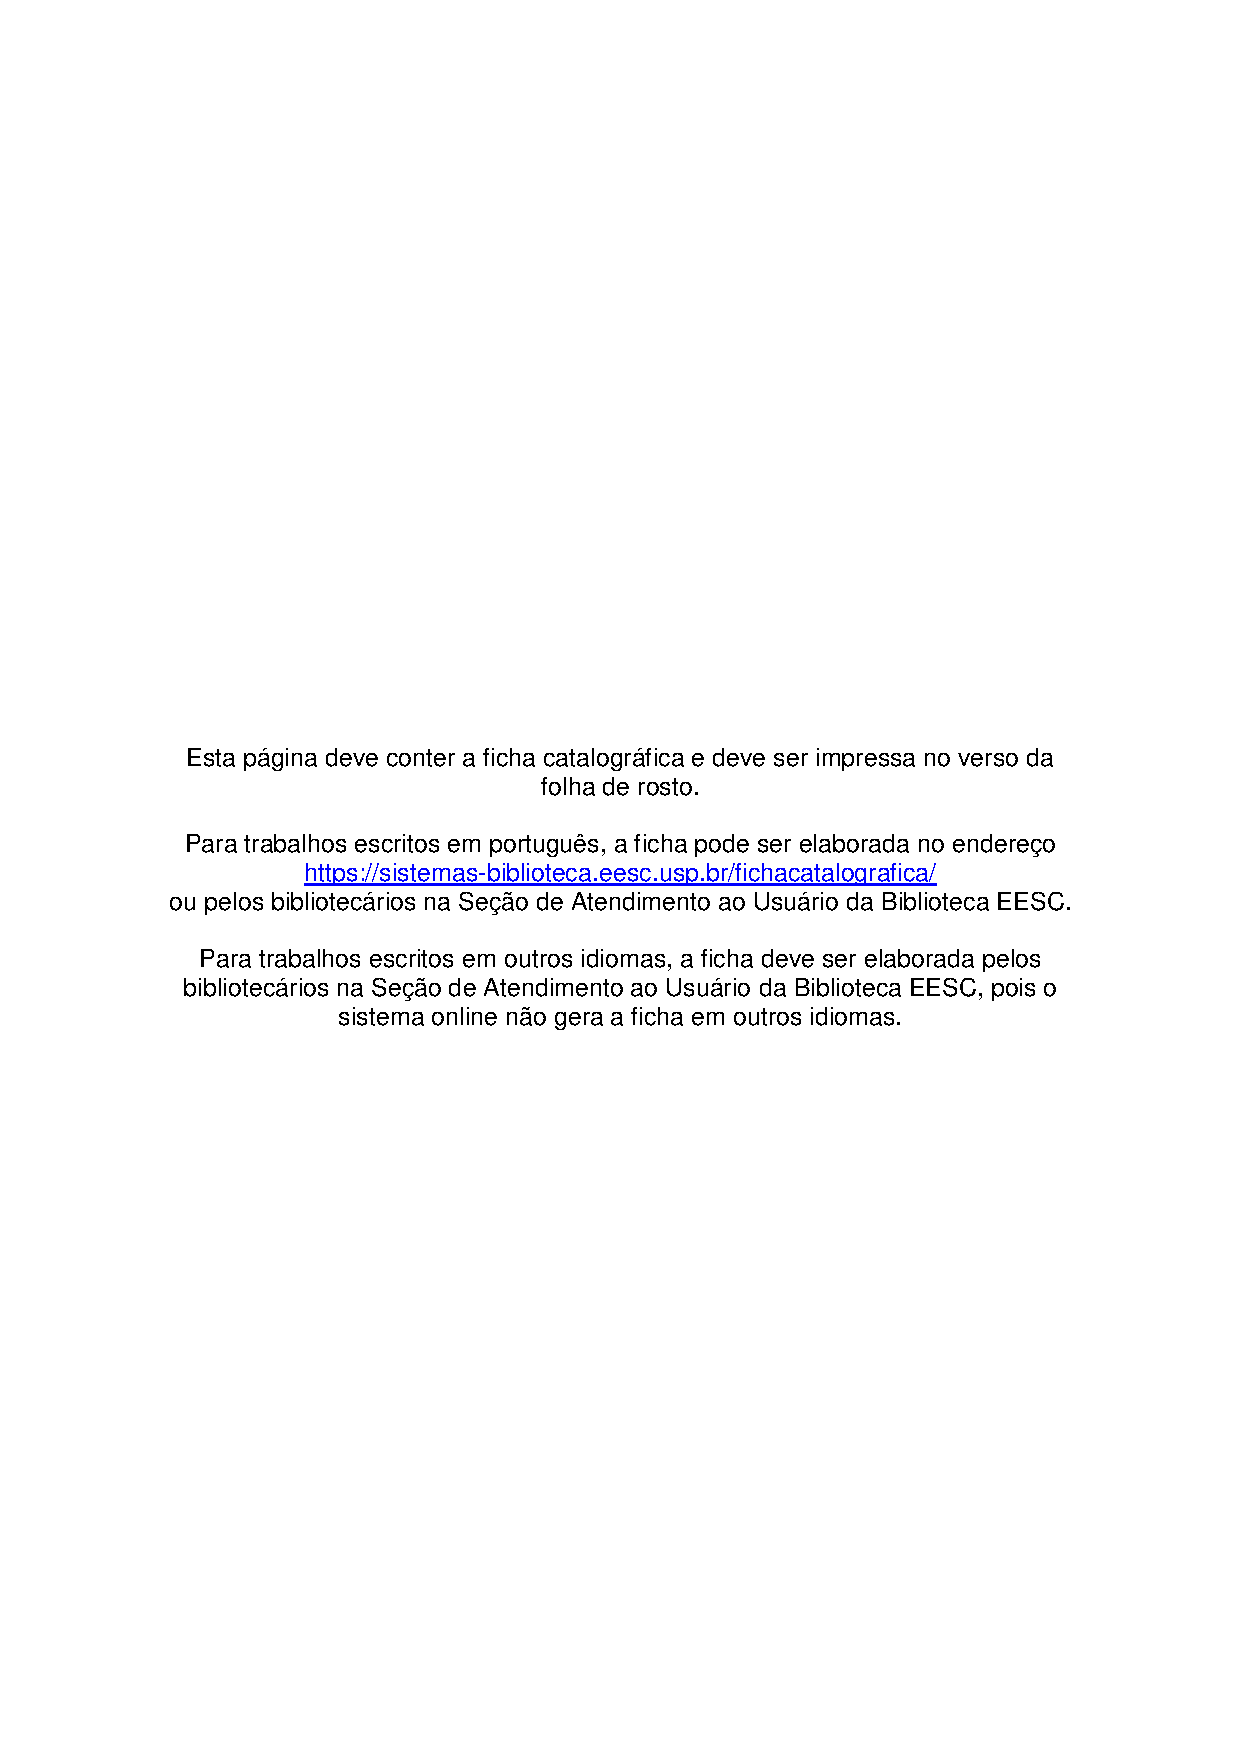
\includepdf{Pre-Textuais/fichacatalografica_latex}
%\chapter*{ERRATA}
Elemento opcional que consiste de uma lista de erros da obra, precedidos pelas folhas e linhas onde eles ocorrem e seguidos pelas correções correspondentes.
\\
% Este é o exemplo presente no documento do ABNTeX2

\begin{table}[ht]
    \centering
    \footnotesize
   \begin{tabular}{|p{1.4cm}|p{1cm}|p{3cm}|p{3cm}|} \hline
    \multicolumn{4}{|c|}{Errata} \\ \hline
       \textbf{Folha}  & \textbf{Linha} & \textbf{Onde se lê} & \textbf{Leia-se} \\ \hline 
        10 & 20 & A & B \\ \hline
        30 &  1  & Elemento optional  & Elemento opcional \\ \hline
        53 &  5  &  Caracteríscas & Características \\ \hline
           &     &                &                 \\ \hline 
           &     &                &                 \\ \hline 
           &     &                &                 \\ \hline 
           &     &                &                 \\ \hline 
    \end{tabular}
    \label{tab:my_label}
\end{table}


%\cleardoublepage

% Folha de avaliação ou aprovação
%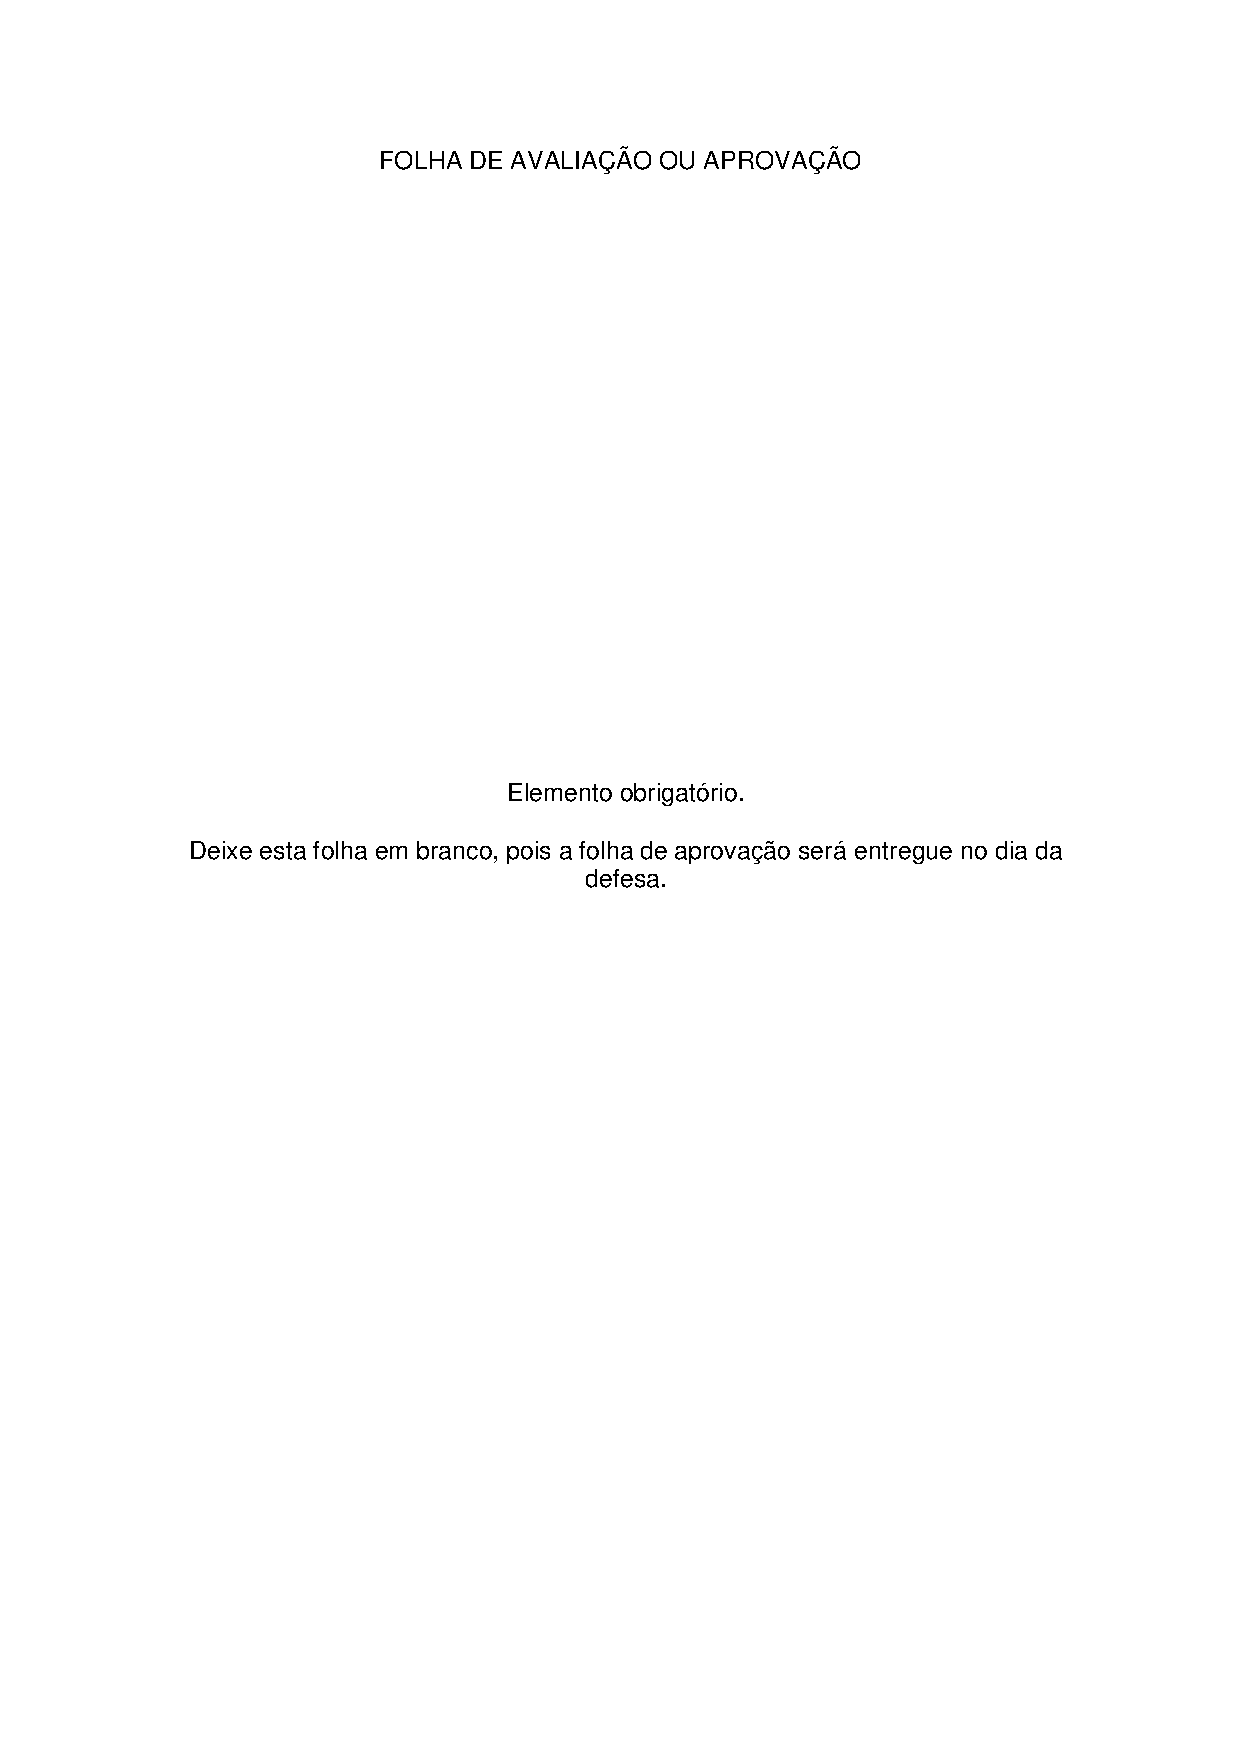
\includepdf{Pre-Textuais/folhadeavaliacao_latex}
%\cleardoublepage

%\begin{dedicatoria}
   \vspace*{\fill}
   \begin{flushright}
      \textit{Este trabalho é dedicado às crianças adultas que,\\
   quando pequenas, sonharam em se tornar cientistas.} %\vspace*{\fill}    
   \end{flushright}
\end{dedicatoria}



%\begin{agradecimentos}

    Gostaria de agradecer primeiramente a Deus por me proporcionar a oportunidade de realizar o mestrado e me por dar forças para superar esse período.

    Os meus mais profundos agradecimentos à minha mãe, Dulce Aline Haubert Yokomizo, e ao meu pai, Tsuyoshi Yokomizo, por todo o amor e carinho que me deram ao longo de toda minha vida. Todo o apoio que me deram foi fundamental para que eu pudesse chegar até aqui. Agradeço também ao meu irmão, Kenzo Haubert Yokomizo, que me escutou em meus momentos bons e ruins. Sem vocês nada disso teria sido possível, amo vocês.

    Agradeço ao meu orientador, professor Dr. Rodolfo André Kuche Sanches, por me proporcionar uma excelente orientação durante todo o mestrado. Muito obrigado por todo o apoio, paciência e dedicação que teve comigo durante esse período.

    Agradeço aos meus amigos, especialmente à Katriny Kauany Amaral dos Santos e ao Evandro Ceciliano Mazer pelo apoio, conselhos e momentos de descontração que temos juntos.

    Agradeço também aos meus amigos do Departamento de Engenharia de Estruturas (SET), que me ajudaram tanto em aspectos técnicos quanto emocionais. Vocês tornaram todo o processo muito mais leve e divertido.

    Ao SET, pela infraestrutura fornecida para a realização do trabalho, assim como aos funcionários pelo ótimo atendimento e auxílio que me deram.

    Por fim, agradeço ao Conselho Nacional de Desenvolvimento Científico e Tecnológico (CNPq) pela bolsa concedida para o desenvolvimento da pesquisa.

\end{agradecimentos}
%\begin{epigrafe}
    \vspace*{\fill}
	\begin{flushright}
		\textit{``Líderes são mestres em encontrar sentido e \\
		aprendizado em todo tipo de experiência de vida.''\\
		\cite[p.~94]{juca2014}}
	\end{flushright}
\end{epigrafe}
\setlength{\absparsep}{18pt} % ajusta o espaçamento dos parágrafos do resumo
\begin{resumo}
  \begin{flushleft}
    \setlength{\absparsep}{0pt} % ajusta o espaçamento da referência	
    \SingleSpacing
    \Autorabr\ \textbf{\Titulo}.	\the\year. \pageref{LastPage}f.
    %Substitua p. por f. quando utilizar oneside em \documentclass
    %\pageref{LastPage}f.
    \Tipotrabalho\ - \Unidademin, \Universidade, \Local, \the\year.
  \end{flushleft}
  \OnehalfSpacing

  O estudo de Interação Fluido-Estrutura está tendo um grau de importância cada vez maior, uma vez que as estruturas estão se tornando cada vez mais leves e esbeltas, devido aos constantes avanços nas diversas áreas da engenharia. Dentre essas interações, enfatiza-se aquelas em que o fluido se encontra em escoamento turbulento, o que ocorre, por exemplo, em edifícios sujeitos à ação de ventos. Sendo assim, se torna necessário o desenvolvimento de técnicas cada vez mais eficientes na determinação do comportamento tanto da estrutura, quanto do escoamento dos fluidos que interagem com a mesma. Nesse sentido, observa-se a existência de uma grande variedade técnicas para determinação do comportamento de estruturas flexíveis, sendo as mais notáveis aquelas baseadas no Método dos Elementos Finitos. Dentre esses métodos, um que está ganhando destaque é aquele que considera posições nodais como parâmetros de análise, denominado de Método dos Elementos Finitos Posicional. Da mesma forma, observa-se que análise de escoamentos também pode ser realizada de diversas maneiras, tais como: construção de amostras em escalas para ensaios práticos; e a modelagem de problemas via métodos matemáticos. Nesse contexto, verifica-se que a construção de amostras reais em escala é muito dispendiosa no ponto de vista de ser necessária uma grande infraestrutura para obtenção de dados válidos, assim como, em alguns casos, os dados obtidos serem dependentes da escala da amostra, não apontando resultados reais, por consequência. Sendo assim, os modelos matemáticos se tornam a melhor solução para se analisar esses problemas. Porém, a depender do grau de complexidade do problema e/ou do modelo empregado, essa análise leva a um custo computacional muito elevado, inviabilizando sua resolução. Dessa forma, o presente trabalho busca realizar um estudo comparativo entre algumas das técnicas mais comuns de análise de Interação Fluido-Estrutura, tais como \RANS, \LES\ e \VMS, considerando escoamentos turbulentos em estruturas flexíveis, empregando o Método dos Elementos Finitos Posicional para essa avaliação.

  \textbf{Palavras-chave:} Interação Fluido-Estrutura. Escoamento Turbulento. Método dos Elementos Finitos Posicional. \textit{Large Eddy Simulation}. \textit{Variational Multi-Scale Methods}. \textit{Reynolds-Averaged Navier-Stokes}.
\end{resumo}

% resumo em inglês
\begin{resumo}[Abstract]
    \begin{otherlanguage*}{english}
        \begin{flushleft}
            \setlength{\absparsep}{0pt} % ajusta o espaçamento da referência	
            \SingleSpacing
            \Autorabr\ \textbf{\Title}.	\the\year. \pageref{LastPage}f.
            %Substitua p. por f. quando utilizar oneside em \documentclass
            %\pageref{LastPage}f.
            \Typeofwork\ - \Unidademin, \Universidade, \Local, \the\year.
        \end{flushleft}
        \OnehalfSpacing

        Fluid-Structure Interaction (FSI) problems occur when a flow affects the behavior of the structure immersed in it and vice versa. The analysis of this type of problem is important, since the effects of this interaction can lead to catastrophic failures, such as the collapse of a structure or loss of aircraft control. However, the numerical simulation of FSI has challenges to be overcome, such as the high computational cost involved in the analyses. This cost can be even higher in turbulent flows, resulting in the need to use more refined meshes to capture the occurrence of vortices. In this context, the present work seeks to study and implement the turbulence model Large Eddy Simulation (LES), observing its influence on poorly discretized analyses. To this end, the equations that govern incompressible isothermal flows are presented, focusing on the Arbitrary Lagrangian-Eulerian (ALE) description, which allows independent movement of the reference domain. The numerical solution of the flow is obtained using the Finite Element Method (FEM), which can be stabilized by the SUPG/PSPG formulation or by the variational multiscale model (VMS). The temporal integrator used is the generalized-$\alpha$, which allows easy control of the high-frequency dissipation of the problem. The movement of the mesh is performed by solving the modified Laplace problem, in order to preserve the quality of the mesh. On the other hand, the problems of computational solid dynamics will be analyzed following a position-based FEM approach for shell elements using Reissner-Mindlin kinematics. Finally, the coupling between the different mediums will be achieved through strong partitioned coupling, as it allows the use of independent codes that properly resolve each medium involved. In this way, the numerical examples are compared with those present in the literature, using different stabilization possibilities, whether or not the LES may be applied. Thus, it can be seen that VMS stabilization slightly improves the results compared to SUPG/PSPG stabilization. The application of LES significantly improves the quality of results, especially in problems with high Reynolds numbers. In FSI problems, LES did not have much effect on problems with refined meshes in the region with the highest velocity gradient, however it still improved the method's convergence on coarser meshes.

        \textbf{Keywords}: Fluid-Structure Interaction. Turbulent Flow. Finite Element Method. Large Eddy Simulation. Variational Multi-Scale. Reynolds-Averaged Navier-Stokes.
    \end{otherlanguage*}
\end{resumo}
\cleardoublepage

% Lista de ilustrações (elemento opcional - recomenda-se que sejam elaboradas a partir de 5 itens)
\listoffigures*
\cleardoublepage

% Lista de tabelas (elemento opcional - recomenda-se que sejam elaboradas a partir de 5 itens)
\listoftables*
\cleardoublepage

\begin{siglas}
    \item[ALE] Lagrangiana-Euleriana Arbitrária - \textit{Arbitrary Lagrangian-Eulerian}
<<<<<<< HEAD
    \item[LBB] Ladyzhenskaya-Babuška-Brezzi
    \item[CFD] Dinâmica dos Fluidos Computacional - \textit{Computational Fluid Dynamics}
    \item[CSD] Dinâmica dos Sólidos Computacional - \textit{Computational Solid Dynamics}
    \item[DNS] Simulação Numérica Direta - \textit{Direct Numerical Simulation}
    \item[GLS] Galerkin Least-Squares
    \item[IFE] Interação Fluido-Estrutura
    \item[IP] Problema de Interação - \textit{Interaction Problem}
    \item[LBB] Condições de \textit{Ladyzhenskaya-Babuška-Brezzi}
=======
    \item[CFD] Dinâmica dos Fluidos Computacional - \textit{Computational Fluid Dynamics}
    \item[CSD] Dinâmica dos Sólidos Computacional - \textit{Computational Solid Dynamics}
    \item[DNS] Simulação Numérica Direta - \textit{Direct Numerical Simulation}
    \item[DOF] Graus de liberdade - \textit{Degree Of Freedom}
    \item[GLS] Galerkin Least-Squares
    \item[IFE] Interação Fluido-Estrutura
    \item[IP] Problema de Interação - \textit{Interaction Problem}
    \item[LBB] Ladyzhenskaya-Babuška-Brezzi
>>>>>>> Qualificacao-Resumida
    \item[LES] Simulação de Grandes Vórtices - \textit{Large Eddy Simulation}
    \item[LSIC] \textit{Least-Squares on Incompressibility Constraint}
    \item[MEF] Método dos Elementos Finitos
    \item[PSPG] \textit{Pressure-Stabilizating/Petrov-Galerkin}
    \item[RANS] \textit{Reynolds-Averaged Navier-Stokes}
    \item[RBVMS] \textit{Residual-Based Variational Multi-Scale}
    \item[SGS] \textit{Subgrid-Scales}
    \item[SUPG] \textit{Streamline-Upwind/Petrov-Galerkin}
    \item[SVK] Saint-Venant-Kirchhoff
<<<<<<< HEAD
=======
    \item[TGV] \textit{Taylor-Green Vortex}
>>>>>>> Qualificacao-Resumida
    \item[VMS] Métodos Variacionais Multiescala - \textit{Variational Multi-Scale}
\end{siglas}
\begin{simbolos}
    \item[\textbf{Operadores}]
    \item[$\dev(\cdot)$] Parte desviadora do tensor
    \item[$\det{(\cdot)}$] Determinante
    \item[$D(\cdot)/Dt$] Derivada material
    \item[$H^1$] Espaço de Sobolev de ordem 1
    \item[$\script{H}(\cdot)$] Matriz Hessiana ($\Ny\otimes\Ny(\cdot)$)
    \item[$L^2$] Espaço das funções de quadrado integrável
    \item[$\tr(\cdot)$] Traço de um tensor
    \item[$\BB{\nabla}(\cdot)$] Gradiente
    \item[$\BB{\nabla}\cdot(\cdot)$] Divergente
    \item[$\BB{\nabla}^2(\cdot)$] Laplaciano
    \item[$\cdot$] Produto interno
    \item[$:$] Contração dupla
    \item[$\vdots$] Contração tripla
    \item[$\times$] Produto vetorial
    \item[$\otimes$] Produto tensorial
    \item[$\sum$] Somatório
    \item[$\prod$] Produtório
    \item[$\norm{(\cdot)}$] Norma

    \item[\textbf{Parâmetros Gerais}]
    \item[$\BB{c}$] Força de corpo
    \item[$\Fres$] Resultante das forças externas
    \item[$\mathbb{I}$] Tensor identidade de quarta ordem
    \item[$\BB{I}$] Tensor identidade de segunda ordem
    \item[$m$] Massa
    \item[$\BB{n}$] Vetor normal à superfície na configuração atual
    \item[$\BB{n}_0$] Vetor normal à superfície na configuração inicial
    \item[$N_a$] Função de forma associada ao nó $a$
    \item[$n_{sd}$] Número de dimensões espaciais do problema
    \item[$t$] Tempo
    \item[$V$] Volume
    \item[$V_0$] Volume inicial
    \item[$\Delta t$] Intervalo discreto de tempo
    \item[$\BB{\xi}$] Coordenada paramétrica
    \item[$\rho$] Massa específica
    \item[$\BB{\sigma}$] Tensor de tensões de Cauchy
    \item[$\phi$] Propriedade qualquer

    \item[\textbf{Configurações do Contínuo}]
    \item[$\fmc$] Função mudança de configuração de $\Omega_0\to\Omega$
    \item[$\tfmc$] Função mudança de configuração de $\Omega_0\to\hat{\Omega}$
    \item[$\hfmc$] Função mudança de configuração de $\hat{\Omega}\to\Omega$
    \item[$\fmc^0$] Função mudança de configuração de $\Omega_\xi\to\Omega_0$
    \item[$\fmc^1$] Função mudança de configuração de $\Omega_\xi\to\Omega$
    \item[$\FMC$] Gradiente da função de mudança de configuração
    \item[$\TFMC$] Gradiente da função $\tfmc$
    \item[$\HFMC$] Gradiente da função $\hfmc$
    \item[$\FMC^0$] Gradiente da função $\fmc^0$
    \item[$\FMC^1$] Gradiente da função $\fmc^1$
    \item[$\BB{x}$] Posição inicial (ou posição material)
    \item[$\BB{\hat{x}}$] Posição de referência
    \item[$\BB{y}$] Posição atual (ou posição espacial)
    \item[$\Gamma$] Fronteira do domínio de análise
    \item[$\Gamma_D$] Fronteira de Dirichlet
    \item[$\Gamma_N$] Fronteira de Neumann
    \item[$\Omega$] Domínio de análise na configuração atual
    \item[$\Omega_0$] Domínio de análise na configuração inicial
    \item[$\Omega_\xi$] Domínio de análise no espaço paramétrico
    \item[$\hat{\Omega}$] Domínio de análise na configuração de referência

    \item[\textbf{Dinâmica dos Fluidos Computacional}]
    \item[$\BB{\mathfrak{D}}$] Tensor constitutivo de quarta ordem
    \item[$\BB{f}$] Força por unidade de massa
    \item[$\BB{g}$] Velocidades prescritas na fronteira de Dirichlet
    \item[$\BB{h}$] Forças de superfícies prescritas na fronteira de Neumann
    \item[$p$] Campo de pressões
    \item[$q$] Função teste relacionado à equação da continuidade
    \item[$\BB{q}$] Resultante das forças externas por unidade de volume
    \item[$\Rey$] Número de Reynolds
    \item[$\script{S}_u$] Espaço de funções tentativas para o campo de velocidades
    \item[$\script{S}_p$] Espaço de funções tentativas para o campo de pressões
    \item[$\BB{u}$] Campo de velocidades
    \item[$\BB{\hat{u}}$] Campo de velocidades da malha
    \item[$\tilde{\BB{u}}$] Velocidade da malha em relação à configuração inicial
    \item[$\dot{\BB{u}}$] Campo de acelerações
    \item[$\script{V}_u$] Espaço de funções teste para o campo de velocidades
    \item[$\script{V}_p$] Espaço de funções teste para o campo de pressões
    \item[$\BB{w}$] Função teste relacionada à equação da conservação do momento
    \item[$\BB{\dot{\varepsilon}}$] Tensor de taxa de deformação
    \item[$\mu$] Viscosidade dinâmica
    \item[$\nu$] Viscosidade cinemática
    \item[$\tau$] Tensor de tensões desviadoras

    \item[\textbf{Dinâmica dos Sólidos Computacional}]
    \item[$\BB{c}^0$] Forças de corpo na configuração inicial
    \item[$\BB{C}$] Tensor de alongamento à direita de Cauchy-Green
    \item[$\tensCon$] Tensor constitutivo de quarta ordem
    \item[$E$] Módulo de elasticidade longitudinal (ou Módulo de Young)
    \item[$\mathbb{E}$] Medida de deformação de Green-Lagrange
    \item[$\BB{F}_a$] Força concentrada sobre o nó $a$
    \item[$G$] Módulo de elasticidade transversal
    \item[$h_0$] Espessura inicial da casca
    \item[$\BB{H}$] Matriz Hessiana
    \item[$J$] Jacobiano da mudança de configuração
    \item[$\mathbb{K}$] Energia cinética
    \item[$\mathbb{P}$] Energia das Forças Externas
    \item[$\BB{P}$] Tensor de tensões de Piola-Kirchhoff de primeira espécie
    \item[$\Stens$] Tensor de tensões de Piola-Kirchhoff de segunda espécie
    \item[$S_0$] Área da superfície na configuração inicial
    \item[$S$] Área da superfície na configuração atual
    \item[$\BB{t}$] força distribuída sobre a superfície média
    \item[$u_e$] Energia específica de deformação
    \item[$\mathbb{U}$] Energia de deformação
    \item[$\BB{w}^0$] Vetor unitário normal à superfície média na configuração inicial
    \item[$\BB{w}^1$] Vetor generalizado na configuração atual
    \item[$\BB{x}^m$] Coordenada inicial de um ponto na superfície média
    \item[$\BB{y}^m$] Coordenada atual de um ponto na superfície média
    \item[$\dot{\BB{y}}$] Campo de velocidades
    \item[$\ddot{\BB{y}}$] Campo de acelerações
    \item[$\alpha$] Taxa de variação da espessura
    \item[$\res$] Vetor resíduo
    \item[$\BB{\varepsilon}$] Tensor de deformação linear
    \item[$\varepsilon_V$] Deformação volumétrica
    \item[$\lambda_m$] Constante de amortecimento
    \item[$\nu$] Coeficiente de Poisson
    \item[$\Pi$] Energia total
    \item[$\DOF$] Vetor que contém todos os graus de liberdade do problema

    \item[\textbf{Acoplamento Fluido-Estrutura}]
    \item[$\script{G}$] Soma de todas as equações diferenciais do problema
    \item[$\BB{H}$] Matriz tangente
    \item[$\BB{h}$] Vetor resíduo
    \item[$\BB{\alpha}$] Vetor contendo os graus de liberdade
    \item[$\BB{\beta}$] Vetor com graus de liberdade das funções teste

    \item[\textbf{\textit{Variational Multi-Scale}}]
    \item[$\NM$] Vetor de resíduo
    \item[$\NC$] Vetor de resíduo
    \item[$\BB{P}$] Vetor de pressões nodais
    \item[$\rC$] Resíduo da equação da continuidade
    \item[$\rM$] Resíduo da equação da conservação da quantidade de movimento
    \item[$\BB{U}$] Vetor de velocidades nodais
    \item[$\dot{\BB{U}}$] Vetor de acelerações nodais
    \item[$\nu_\lsic$] Estabilizador LSIC
    \item[$\rho_\infty$] Raio espectral
    \item[$\tau_\sups$] Estabilizador SUPS
    \item[$\bar{\phi}$] Valor de uma propriedade no subespaço de escalas grosseiras
    \item[$\phi'$] Valor de uma propriedade no subespaço de escalas finas

    \item[\textbf{\textit{Large Eddy Simulation}}]
    \item[$\BB{C}$] Tensor de termos cruzados
    \item[$C_S$] Constante de Smagorinsky
    \item[$\Dfil$] Domínio de abrangência do filtro
    \item[$E(k)$] Amplitude espectral da energia cinética
    \item[$g$] Filtro
    \item[$k$] Raio da esfera parametrizada
    \item[$\BB{L}$] Tensor de Leonard
    \item[$\BB{R}$] Tensor SGS de Reynolds
    \item[$\deffil$] Taxa de deformação em grandes escalas
    \item[$\BB{T}$] Tensor SGS
    \item[$\BB{T}_S$] Tensor SGS de Smagorinsky
    \item[$\yfil$] Ponto na vizinhança de $\BB{y}$ interno à $\Dfil$
    \item[$\alpha$] Constante de Kolmogoroff
    \item[$\Delta$] Tamanho da malha
    \item[$\ep$] Dissipação turbulenta
    \item[$\nu_T$] Viscosidade de vórtice
    \item[$\bar{\phi}$] Propriedade filtrada
    \item[$\phi'$] Propriedade não filtrada

    \item[\textbf{\textit{Reynolds-Averaged Navier-Stokes}}]
    \item[$\BB{b}$] Tensor de tensões anisotrópico de Reynolds
    \item[$\BB{C}$] Gradiente de difusão turbulenta
    \item[$D_\ep$] Difusão turbulenta
    \item[$k$] Energia cinética média gerada pelo campo de flutuações
    \item[$\script{P}$] Pressão dividida pela massa específica
    \item[$\BB{P}$] Produção do tensor de Reynolds
    \item[$P_\ep$] Produção da dissipação
    \item[$\ep$] Dissipação turbulenta da energia cinética
    \item[$\BB{\ep}$] Tensor de taxa de dissipação turbulenta da energia cinética
    \item[$\BB{\Pi}$] Correlação entre pressão e o tensor de taxa de deformação do campo de flutuações
    \item[$\bar{\phi}$] Média temporal de uma propriedade
    \item[$\phi'$] Flutuação de uma propriedade no espaço-tempo
    \item[$\Phi_\ep$] Destruição turbulenta da dissipação
    \item[$\BB{\tau}$] Tensor de tensões de Reynolds
    \item[$\omega$] Escala de tempo turbulento
\end{simbolos}

% Sumário
\pdfbookmark[0]{\contentsname}{toc}
\tableofcontents*
\cleardoublepage

\textual
% \pagestyle{simple} % tira cabeçalho com nome do capítulo e exibe só paginação

%==================================================================================================
\chapter{Introdução}
%==================================================================================================

Problemas de interação fluido-estrutura (IFE) referem-se a situações nas quais a presença de um escoamento afeta o comportamento de uma estrutura, e vice-versa. Essa interação pode ocorrer devido ao desenvolvimento de um campo de pressões devido ao escoamento, que por sua vez solicita a estrutura, fazendo-a se deslocar, influenciando, consequentemente, o escoamento. Assim, o estudo desse tipo de problema envolve a análise multifísica, em que os diferentes meios físicos (sólido e fluido) são regidos por suas próprias equações constitutivas, e que, por sua vez, interagem entre si. Dessa forma, a análise de IFE apresenta desafios a serem superados, uma vez que envolve grande interdisciplinaridade, tanto para descrever adequadamente o comportamento dos meios físicos, quanto para se descrever como se dá essa interação.

A interação entre fluidos e estruturas é um fenômeno que ocorre em diversas situações, como em turbinas eólicas, pontes, edifícios de grande altitudes, estruturas \textit{offshore}, aeronaves, escoamento em vasos sanguíneos, entre outros. A análise desses problemas é de grande importância, uma vez que a interação entre fluidos e estruturas pode levar a falhas catastróficas, como o colapso de pontes ou edifícios, ou a perda de controle de uma aeronave.

Já em relação à classificação dos escoamentos, estes podem ser classificados, dentre outras formas, em função do número de Reynolds, o qual é um coeficiente adimensional definido como a razão entre as forças inerciais e as forças viscosas. Assim, os escoamentos podem ser classificados, a depender desse coeficiente, em 3 tipos: escoamento laminar; de transição; e turbulento. No primeiro caso, o escoamento se dá de forma similar ao escorregamento de lâminas paralelas entre si, sem que haja uma mistura macroscópica entre elas. Já no segundo caso começam a surgir algumas flutuações esporádicas no escoamento, porém ainda não se apresentam de forma tão significativa a considerá-lo turbulento. O último caso apresenta flutuações constantes em seu fluxo, resultando no surgimento de estruturas denominadas de vórtices.

Assim, em casos de escoamentos turbulentos, pode-se ocorrer o aumento do arrasto sobre a estrutura, desprendimento de vórtices, vibrações induzidas pelo escoamento, entre outros. Também pode-se ocorrer queda do coeficiente de sustentação de aerofólios, devido à formação de bolhas de desprendimento.

Com isso, pode-se partir para diferentes abordagens para obtenção de resultados para problemas de IFE. Uma delas é a abordagem experimental, que consiste na construção de modelos em escala reduzida para ensaios em túneis de ventos, canais ou tanques de ensaio. No entanto, essa abordagem apresenta limitações, uma vez que demandam grandes investimentos com infraestrutura, assim como a construção de modelos em escala reduzida pode não capturar todos os fenômenos físicos que ocorrem em um escoamento real, além de possuir pouca flexibilidade quanto aos modelos ensaiados \cite{fernandes2020tecnica}.

Outra abordagem possível é a abordagem teórica. Nesse caso, a formulação matemática dos problemas de IFE é conduzida de forma que ambos os meios sejam devidamente acoplados. No entanto, a resolução de problemas dessa natureza demanda a solução de sistemas de equações diferenciais parciais (EDP) cuja solução é desconhecida para a maioria dos problemas, e quando conhecida, é restrita a problemas pequenos e com muitas hipóteses simplificadoras, sem muita representatividade em problemas reais.% Tais dificuldades são ainda potencializadas quando a estrutura desenvolve grandes deslocamentos, ou o escoamento passa a ser dominado pela convecção, o que torna o caráter da solução altamente não-linear.

Dessa forma, a utilização de métodos numéricos se mostra como uma alternativa viável, uma vez que são capazes de resolver tais sistemas de equações de maneira aproximada mantendo-se, mesmo assim, a boa representatividade de sua solução. Dentre os métodos numéricos disponíveis para isso, destaca-se o Método dos Elementos Finitos (MEF), o qual parte da subdivisão de domínios contínuos em elementos constituídos por nós, que por sua vez possuem intrinsecamente valores associados às variáveis do problema. Assim, ao invés de procurar uma solução na forma forte do problema, essa abordagem busca soluções na forma fraca. Com isso o problema resume-se à busca de uma solução de um sistema algébrico de equações. Esse método é amplamente empregado na dinâmica dos sólidos computacional (CSD), e que tem ganhado cada vez mais espaço também na dinâmica dos fluidos computacional (CFD). Algumas características verificadas nesse método, que conferem eficiência, são a possibilidade de se modelar problemas de geometria complexa, aplicar condições de contorno de maneira simples, assim como poder trabalhar com diferentes materiais em uma mesma simulação. Portanto, problemas de IFE abordados segundo o MEF devem tratar de três áreas de estudo: a mecânica dos sólidos, a mecânica dos fluidos e os problemas de interação (IP).

Geralmente, a formulação que baseia o MEF no contexto da mecânica dos sólidos parte de princípios energéticos, os quais buscam a conservação da energia. Sendo assim, diferentes formas de se obter soluções são desenvolvidas, como o MEF corrotacional, o qual decompõe o movimento em parcelas de movimento de corpo rígido e de deformação, além de considerar como variáveis nodais (ou graus de liberdade - DOF) os deslocamentos e rotações nodais. No entanto a utilização de rotações finitas e uma matriz de massa variável dificultam sua aplicação, além de torná-lo mais apropriado a problemas de pequenos deslocamentos \cite{sanches2013unconstrained}. Sendo assim, alternativas como o MEF baseado em posições, proposto por \citeonline{coda2003analise}, se torna mais viável, uma vez que já traz naturalmente a consideração de não linearidade geométrica, além de possuir uma matriz de massa constante, facilitando, assim, sua aplicação.

Já no contexto de CFD, o MEF tem se mostrado como uma alternativa viável para a resolução de problemas de escoamentos. No entanto, a utilização de elementos clássicos de Galerkin, o qual considera igualmente as parcelas de derivadas tanto à jusante quanto à montante, o que leva à resultados espúrios em problemas de convecção dominante. Sendo assim, uma possibilidade de se contornar esse problema está na aplicação de técnicas de estabilização, como a aplicação do termo SUPG (\SUPG), que, por meio de modificação nas funções ponderadoras, toma uma contribuição maior das derivadas à montante do escoamento, estabilizando a solução na direção das linhas de corrente.

Além disso, os espaços de aproximação para a pressão em problemas de escoamentos incompressíveis também podem ser fonte de instabilidade numérica. Dessa forma, a fim de se obter um sistema definido, é necessária a adoção de elementos mistos que atendam às condições de \LBB\ (LBB), as quais impedem a escolha dos mesmos espaços aproximadores para os campos de velocidades e pressões. Assim, alguns elementos mistos são possíveis, como os elementos Taylor-Hood, que são capazes de atender às condições LBB, e que são largamente utilizados em problemas de escoamentos incompressíveis. No entanto, buscando uma maior flexibilidade na escolha dos espaços aproximadores, alguns trabalhos têm proposto a utilização de técnicas de estabilização para a pressão, como a técnica PSPG (\PSPG).

De maneira mais ampla, é possível partir para métodos de estabilização multiescala, como a técnica de estabilização VMS (\VMS), que busca estabilizar a solução nas diferentes escalas do escoamento. A partir da decomposição dos campos de velocidades e pressões em parcelas de grandes e pequenas escalas, a técnica VMS incorpora tanto os termos SUPG e PSPG quanto termos adicionais da própria formulação.

Ademais, conforme o número de Reynolds aumenta, começam a surgir estruturas turbulentas, que se manifestam tridimensionalmente de maneira instável, desordenada e em diversas escalas diferentes. Isso faz com que a obtenção de soluções numéricas desse tipo de fluxo seja uma tarefa muito custosa computacionalmente, uma vez que, para capturar a formação de vórtices até mesmo nas menores escalas, é necessária uma malha muito refinada, assim como algumas simulações possuem um domínio computacional consideravelmente grande. Tal custo torna, portanto, a aplicação do MEF inviável em problemas usuais de engenharia, que em muitos casos exigem respostas mais ágeis para serem utilizadas em elaborações de projetos. Assim, motivados à reduzir o custo computacional, diversos modelos de turbulência têm sido propostos, como os baseados na decomposição de Reynolds (\RANS\ - RANS), ou em grandes vórtices (\LES\ - LES).

Os modelos de turbulência podem ser classificados em três grupos: $i$ - modelos mais simples, que empregam expressões algébricas para descrever a viscosidade turbulenta, assumindo que as estruturas turbulentas são geradas e dissipadas no mesmo local; $ii$ - modelos que adicionam equações diferenciais adicionais para o cálculo da viscosidade turbulenta; e $iii$ - modelos que adicionam equações diferenciais de transporte para o cálculo das tensões de Reynolds \cite{souza2011revisao,alfonsi2009reynolds,teixeira2001simulaccao}.

No caso dos modelos RANS, as variáveis das equações de Navier-Stokes são decompostas em parcelas referentes à sua média e às suas flutuações, sendo que a tomada da média pode ser feita de diferentes formas a depender da natureza do escoamento, como a média temporal, adequada a problemas estacionários, a média espacial, apropriada para escoamentos homogêneos, e a média de um conjunto de experimentos, para casos mais gerais. Os modelos RANS são mais comumente classificados em função da quantidade de equações diferenciais de transporte adicionadas ao problema, como os problemas de zero equações, uma equação, duas equações e os modelos de tensões. Nesse tipo de simulação observa-se a introdução de diversos novos termos e grandezas com as equações adicionais, tal como o tensor de Reynolds e os termos presentes nas equações de transporte escritos em função de campos de flutuação, os quais inserem constantes definidas empiricamente ao problema.

No caso dos modelos LES a decomposição das variáveis é feita a partir de um filtro que separa as grandes estruturas turbulentas das pequenas. A suposição básica desses modelos é que as grandes escalas são responsáveis pelo transporte da energia e da quantidade de movimento, sendo resolvidas diretamente pelas equações de Navier-Stokes filtradas, enquanto as escalas pequenas (\textit{Sub-Grid Scales} - SGS) possuem comportamento isotrópico que, apesar de não poderem ser resolvidas diretamente, sua influência na escala maior pode ser modelada. Dentre as propostas de se modelar as pequenas escalas, é tradicionalmente empregado o modelo de Smagorinsky, o qual relaciona a viscosidade turbulenta com o campo de velocidades em grandes escalas.

Por fim, se tratando dos problemas de interação, vale ressaltar algumas diferenças que podem ocorrer na descrição matemática dos diferentes meios. Tradicionalmente são empregadas a descrição Lagrangiana (ou material) e a descrição Euleriana (ou espacial).

Na descrição Lagrangiana a referência adotada é a configuração inicial do contínuo. Essa descrição apresenta bom desempenho quando aplicada à mecânica dos sólidos, uma vez que a configuração inicial é bem definida e suas deformações são finitas, tendo como variáveis principais os deslocamentos do sólido \cite{sanches2014fluid, fernandes2019ale}. Já a descrição Euleriana toma como referência a configuração atual do contínuo, sendo muito utilizada para a descrição de fluidos newtonianos, pois esses não apresentam resistência às tensões de cisalhamento, distorcendo-se indefinidamente quando submetidos a tais solicitações \cite{sanches2014fluid, fernandes2019ale}.

Assim, é importante que a análise de interação fluido estrutura combine adequadamente a mecânica dos sólidos, convenientemente descrita na forma Lagrangiana, com a mecânica dos fluidos, convenientemente descrita na forma Euleriana. Uma forma robusta de se fazer isso é empregar a descrição Lagrangiana-Euleriana Arbitrária (ALE) \cite{donea1982arbitrary} para o fluido. Essa descrição considera um domínio de referência com movimento arbitrário e independente das partículas. Isso permite que a malha do fluido seja movimentada dinamicamente para acomodar a movimentação da interface fluido-sólido.

Dessa maneira, visando a identificação de uma formulação eficiente para simular de problemas de interação fluido-estrutura com escoamentos turbulentos, esta proposta trata da implementação do modelo de turbulência LES baseado no modelo de viscosidade de Smagorinsky, bem como da formulação VMS em um programa para escoamentos incompressíveis com contornos móveis (empregando descrição ALE), do acoplamento da ferramenta resultante com um programa para análise dinâmica de cascas com grandes deslocamentos, e com a finalidade de se estudar o desempenho desses modelos em simulação de problemas numéricos para estudo e verificação das implementações. Os estudos numéricos deverão tomar como referência tanto a solução direta (sem modelo de turbulência) obtida pela ferramenta computacional desenvolvida, bem como resultados disponíveis na literatura.

Com isso, o trabalho busca trazer uma maior compreensão sobre os impactos que a utilização de modelos de turbulência pode ter em problemas de IFE, bem como a influência das técnicas de estabilização na obtenção de soluções numéricas. Além disso, espera-se desenvolver uma ferramenta computacional que seja capaz de alternar entre diferentes tipos de elementos, técnicas de estabilização e modelo de turbulência em problemas de IFE com escoamentos turbulentos incompressíveis.

%==================================================================================================
\section{Organização Do Trabalho}
%==================================================================================================

A presente dissertação está estruturada em 6 capítulos, os quais são brevemente descritos a seguir.

    {
        \newcommand{\Capi}[2]{\textbf{Capítulo #1 - #2}:}

        \Capi{1}{Introdução} Apresenta a motivação para o desenvolvimento do trabalho, bem como sua importância, objetivos e a justificativa para a realização do mesmo. Para isso se introduz resumidamente as principais características e particularidades dos problemas de interação fluido-estrutura, bem como as dificuldades encontradas para a obtenção de soluções numéricas para esses problemas. Na sequência é apresentado o estado da arte, de forma a situar o leitor quanto ao que já foi desenvolvido na área, para que se tenha uma contextualização sobre o panorama científico atual. Com isso o leitor estará apto a compreender a metodologia proposta e sua justificativa, as quais são apresentadas na sequência.

        \Capi{2}{Formulação Numérica Para Mecânica Dos Fluidos} Inicialmente são apresentadas as equações governantes de escoamentos isotérmicos incompressíveis, tanto na descrição Euleriana, considerando domínios fixos, quanto na descrição Lagrangiana-Euleriana Arbitrária, para domínios móveis. Em seguida é obtida uma formulação semi-discreta das equações governantes, assim como o esquema de integração temporal adotado, com a finalidade de implementação computacional das mesmas. Assim é abordado o modelo de estabilização VMS, onde se comenta também sobre as estabilizações SUPG e PSPG. Em seguida apresenta-se o modelo de turbulência LES, com destaque para o modelo de viscosidade de Smagorinsky. Por fim, são apresentados exemplos de verificação para a formulação numérica proposta.

        \Capi{3}{Formulação Numérica Para Dinâmica Não Linear Dos Sólidos} Apresenta-se primeiramente os conceitos básicos da dinâmica dos corpos deformáveis, onde se introduz as medidas fundamentais para o estudo desses meios, focando na descrição Lagrangiana Total. Com isso torna-se possível apresentar a abordagem energética, assim como o modelo constitutivo adotado para a análise. Dessa maneira restringe-se a análise para elementos de cascas com cinemática de Reissner-Mindlin, onde se parte para uma abordagem posicional do MEF. Finalmente estudam-se alguns exemplos para verificação da formulação.

        \Capi{4}{Movimentação Da Malha Via Suavização De Laplace} Introduz-se uma modificação do esquema de movimentação de Laplace. Nesse esquema resultante os elementos menores da malha possuem uma rigidez maior em relação aos maiores, preservando, assim, a qualidade da malha. Com isso são apresentados exemplos de aplicação da técnica em problemas de IFE com movimento prescrito por parte da estrutura.

        \Capi{5}{Acoplamento Fluido-Estrutura} São apresentadas as condições necessárias para se realizar o acoplamento fluido-estrutura, assim como as técnicas de acoplamento particionado (fraco e forte) e suas particularidades. Dessa forma são estudados problemas de IFE por meio do acoplamento forte em diversas situações (diferentes espaços aproximadores, termos estabilizadores e a utilização, ou não, de modelos de turbulência).

        \Capi{6}{Conclusões} Com base nos resultados obtidos nos capítulos anteriores são apresentadas as conclusões do trabalho e, a partir disso, são propostas sugestões para trabalhos futuros.
    }

%==================================================================================================
% ESTADO DA ARTE
%==================================================================================================

% Introdução

\documentclass[_ArquivoPrincipal.tex]{subfiles}

\begin{document}

%==================================================================================================
\chapter{Estado Da Arte}
%==================================================================================================
	
No presente capítulo serão abordados os principais temas relacionados à problemas de Interação Fluido-Estrutura (IFE), tendo como ênfase os modos de turbulência. Serão destacados os principais métodos de cálculos envolvendo a dinâmica das estruturas computacional (\ref{CSD}), a dinâmica dos fluidos computacional (\ref{CFD}) e alguns modelos de turbulências (\ref{MT}).

%==================================================================================================
\section{Dinâmica Das Estruturas Computacional} \label{CSD}
%==================================================================================================

A mecânica dos sólidos visa a determinação de parâmetros referentes à elementos estruturais sujeitos a solicitações externas, tais como tensões e deformações, ou forças e deslocamentos de determinados pontos dos mesmos. Para isso são desenvolvidos diversos métodos com a finalidade de melhor descrever o comportamento das estruturas, como o Método dos Elementos Finitos (MEF), que se apresenta como a ferramenta computacional mais amplamente utilizada para esse fim.

Nesse sentido vale ressaltar os trabalhos de \citeonline{hughes1981nonlinear, argyris1982excursion, ibrahimbegovic2002role, pimenta2004fully, battini2006choice} e \citeonline{pimenta2008exact}, que realizaram análises através do MEF Corrotacional, que se trata de uma formulação onde os deslocamentos e rotações dos elementos são os parâmetros principais da análise.

No entanto a utilização de uma análise que considera tais parâmetros nodais só se mostra eficiente ao se estudar estruturas que desenvolvem pequenos deslocamentos e deformações. Isso deve-se ao fato de essa abordagem utilizar rotações finitas como parâmetros nodais, o que pode gerar controversas em problemas envolvendo grandes rotações, uma vez que não há comutatividade entre essas grandezas. Ainda observa-se que a avaliação dinâmica de estruturas reticuladas se torna problemática, do ponto de vista da conservação de energia, além da matriz de massa ser variável, tornando o processo de integração temporal muito complexo \cite{sanches2013unconstrained}.

Com isso, vale ressaltar os trabalhos de \citeonline{coda2004simple, coda2007alternative, coda2010improved, coda2009two, coda2009unconstrained} e \citeonline{carrazedo2010alternative} que utilizam de forma bem-sucedida o MEF Posicional para análise de estruturas reticuladas e de cascas aplicadas à grandes deslocamentos. Este método se diferencia dos demais ao considerar as posições nodais, obtidas a partir de vetores indeformados, como parâmetros de análise, facilitando o cálculo de efeitos de não-linearidade geométrica.

\citeonline{sanches2013unconstrained} apresentaram uma aplicação do método dos elementos finitos posicional em elementos de cascas e constataram a presença de uma matriz de massa constante, o que possibilita a utilização de métodos de integração temporal, como o método de Newmark $\beta$, conservando, assim, o momento linear e angular em análises dinâmicas. Além disso, esse trabalho também analisou problemas envolvendo IFE, obtendo resultados favoráveis, indicando a boa aplicação desse método em problemas dessa natureza.

No âmbito da IFE, destaca-se a necessidade dessa consideração, uma vez que são observadas aplicações como, por exemplo, grandes amplitudes de deslocamentos, como \textit{flutter}, aplicações biomecânicas, estruturas infláveis \cite{karagiozis2011computational}, simulações de turbinas \cite{bazilevs20113d}, dentre outras.

%==================================================================================================
\section{Dinâmica Dos Fluidos Computacional} \label{CFD}
%==================================================================================================

Ao contrário de problemas envolvendo elementos sólidos, que possuem um estado inicial bem definido, os fluidos, em especial os Newtonianos, não o possuem, uma vez que não incapazes de resistir à tensões desviadoras, deformando-se, assim, indefinidamente quando sujeitos à essas tensões. Dessa forma, torna-se apropriada a utilização de uma descrição Euleriana para descrever os fluidos, em que os parâmetros nodais são principalmente as velocidades do mesmo \cite{fernandes2020tecnica}.

Em geral, problemas envolvendo Dinâmica dos Sólidos (\textit{Computational Solid Dynamics} - CSD) partem do princípio da estacionariedade de energias, buscando a determinação do ponto em que a energia do sistema seja mínima. Esses métodos apresentam a particularidade de surgir um sistema de equações com uma matriz simétrica e, em alguns casos, de vetores cujas componentes possuem significado físico. Porém, em problemas que envolvem a Dinâmica dos Fluidos (\textit{Computational Fluid Dynamics} - CFD), o sistema de equações possui uma matriz, na maioria dos casos, assimétrica, devido à presença de termos convectivos nas equações governantes \cite{bazilevs2013computational,brooks1982streamline}.

Nesse sentido, são desenvolvidos novos métodos, em busca de uma solução mais representativa com uma malha menos refinada. Dentre os principais desenvolvidos, vale mencionar o \textit{Streamline-Upwind/Petrov-Galerkin} (SUPG) \cite{brooks1982streamline}, \textit{Galerkin Least-Squares} (GLS) \cite{hughes1989new,tezduyar1991stabilized}, \textit{Subgrid Scales} (SGS) e \cite{hughes1995multiscale}.

Um campo que vale destacar na CFD é o que estuda os fenômenos de turbulência, uma vez que esses fenômenos podem se apresentar nas mais variadas escalas, sendo necessário a geração de uma malha muito refinada para detectar a formação dos vórtices, o que ocasiona um aumento radical no custo computacional da análise. Assim, são desenvolvidas novas técnicas afim de se obter melhores resultados, sem que haja um grande aumento no volume de cálculos. Dentre esses métodos destacam-se os métodos multiescala (\textit{Variational Multi-Scale} - VMS), as simulações de grandes vórtices (\textit{Large Eddy Simulation} - LES) \cite{hughes1995multiscale,hughes1998variational,hughes2002variational,bazilevs2010large,vsekutkovski2021partitioned}, aproximações de \textit{Reynolds-Averaged Navier-Stokes} \cite{alfonsi2009reynolds} e os métodos de atualização de malha \cite{de1993petrov}. O capítulo \ref{FT} descreve de forma mais detalhada cada um desses métodos.

%==================================================================================================
\section{Interação Fluido-Estrutura} \label{IFE}
%==================================================================================================

\textcolor{red}{TEXTO}

%==================================================================================================
\section{Modelo De Turbulência} \label{MT}
%==================================================================================================

Um fluido pode apresentar um escoamento de duas formas distintas, a depender do número de Reynolds que este apresenta (conforme ilustrado na Figura \ref{fig:Escoamentos}). Em casos cujo número de Reynolds é baixo, o escoamento é considerado laminar, ou seja, o escoamento se dá de forma semelhante ao movimento de lâminas independentes, não havendo mistura macroscópica entre as mesmas. Esse tipo de escoamento possui soluções muito mais simples de se obter, no entanto representam uma ocorrência baixa na maioria dos problemas observados na natureza. Já em casos cujo número de Reynolds é muito elevado, o escoamento é considerado turbulento. Nesse cenário há a formação de vórtices sobre o escoamento, que podem ocorrer de forma instável, desordenada e em várias escalas diferentes \cite{popiolek2005analise,shaughnessy2005introduction}. Esse fenômeno pode ser descrito de acordo com as equações de Navier-Stokes, no entanto sua resolução se apresenta com um alto grau de complexidade, uma vez que possui termos não lineares em sua composição. Assim são necessárias técnicas de solução, para que se possa obter uma solução de forma aproximada à essas equações.

\begin{figure}[h]
    \centering
    \caption{Esquema de escoamentos.\label{fig:Escoamentos}}
    \begin{subfigure}{.45\textwidth}
        \centering
        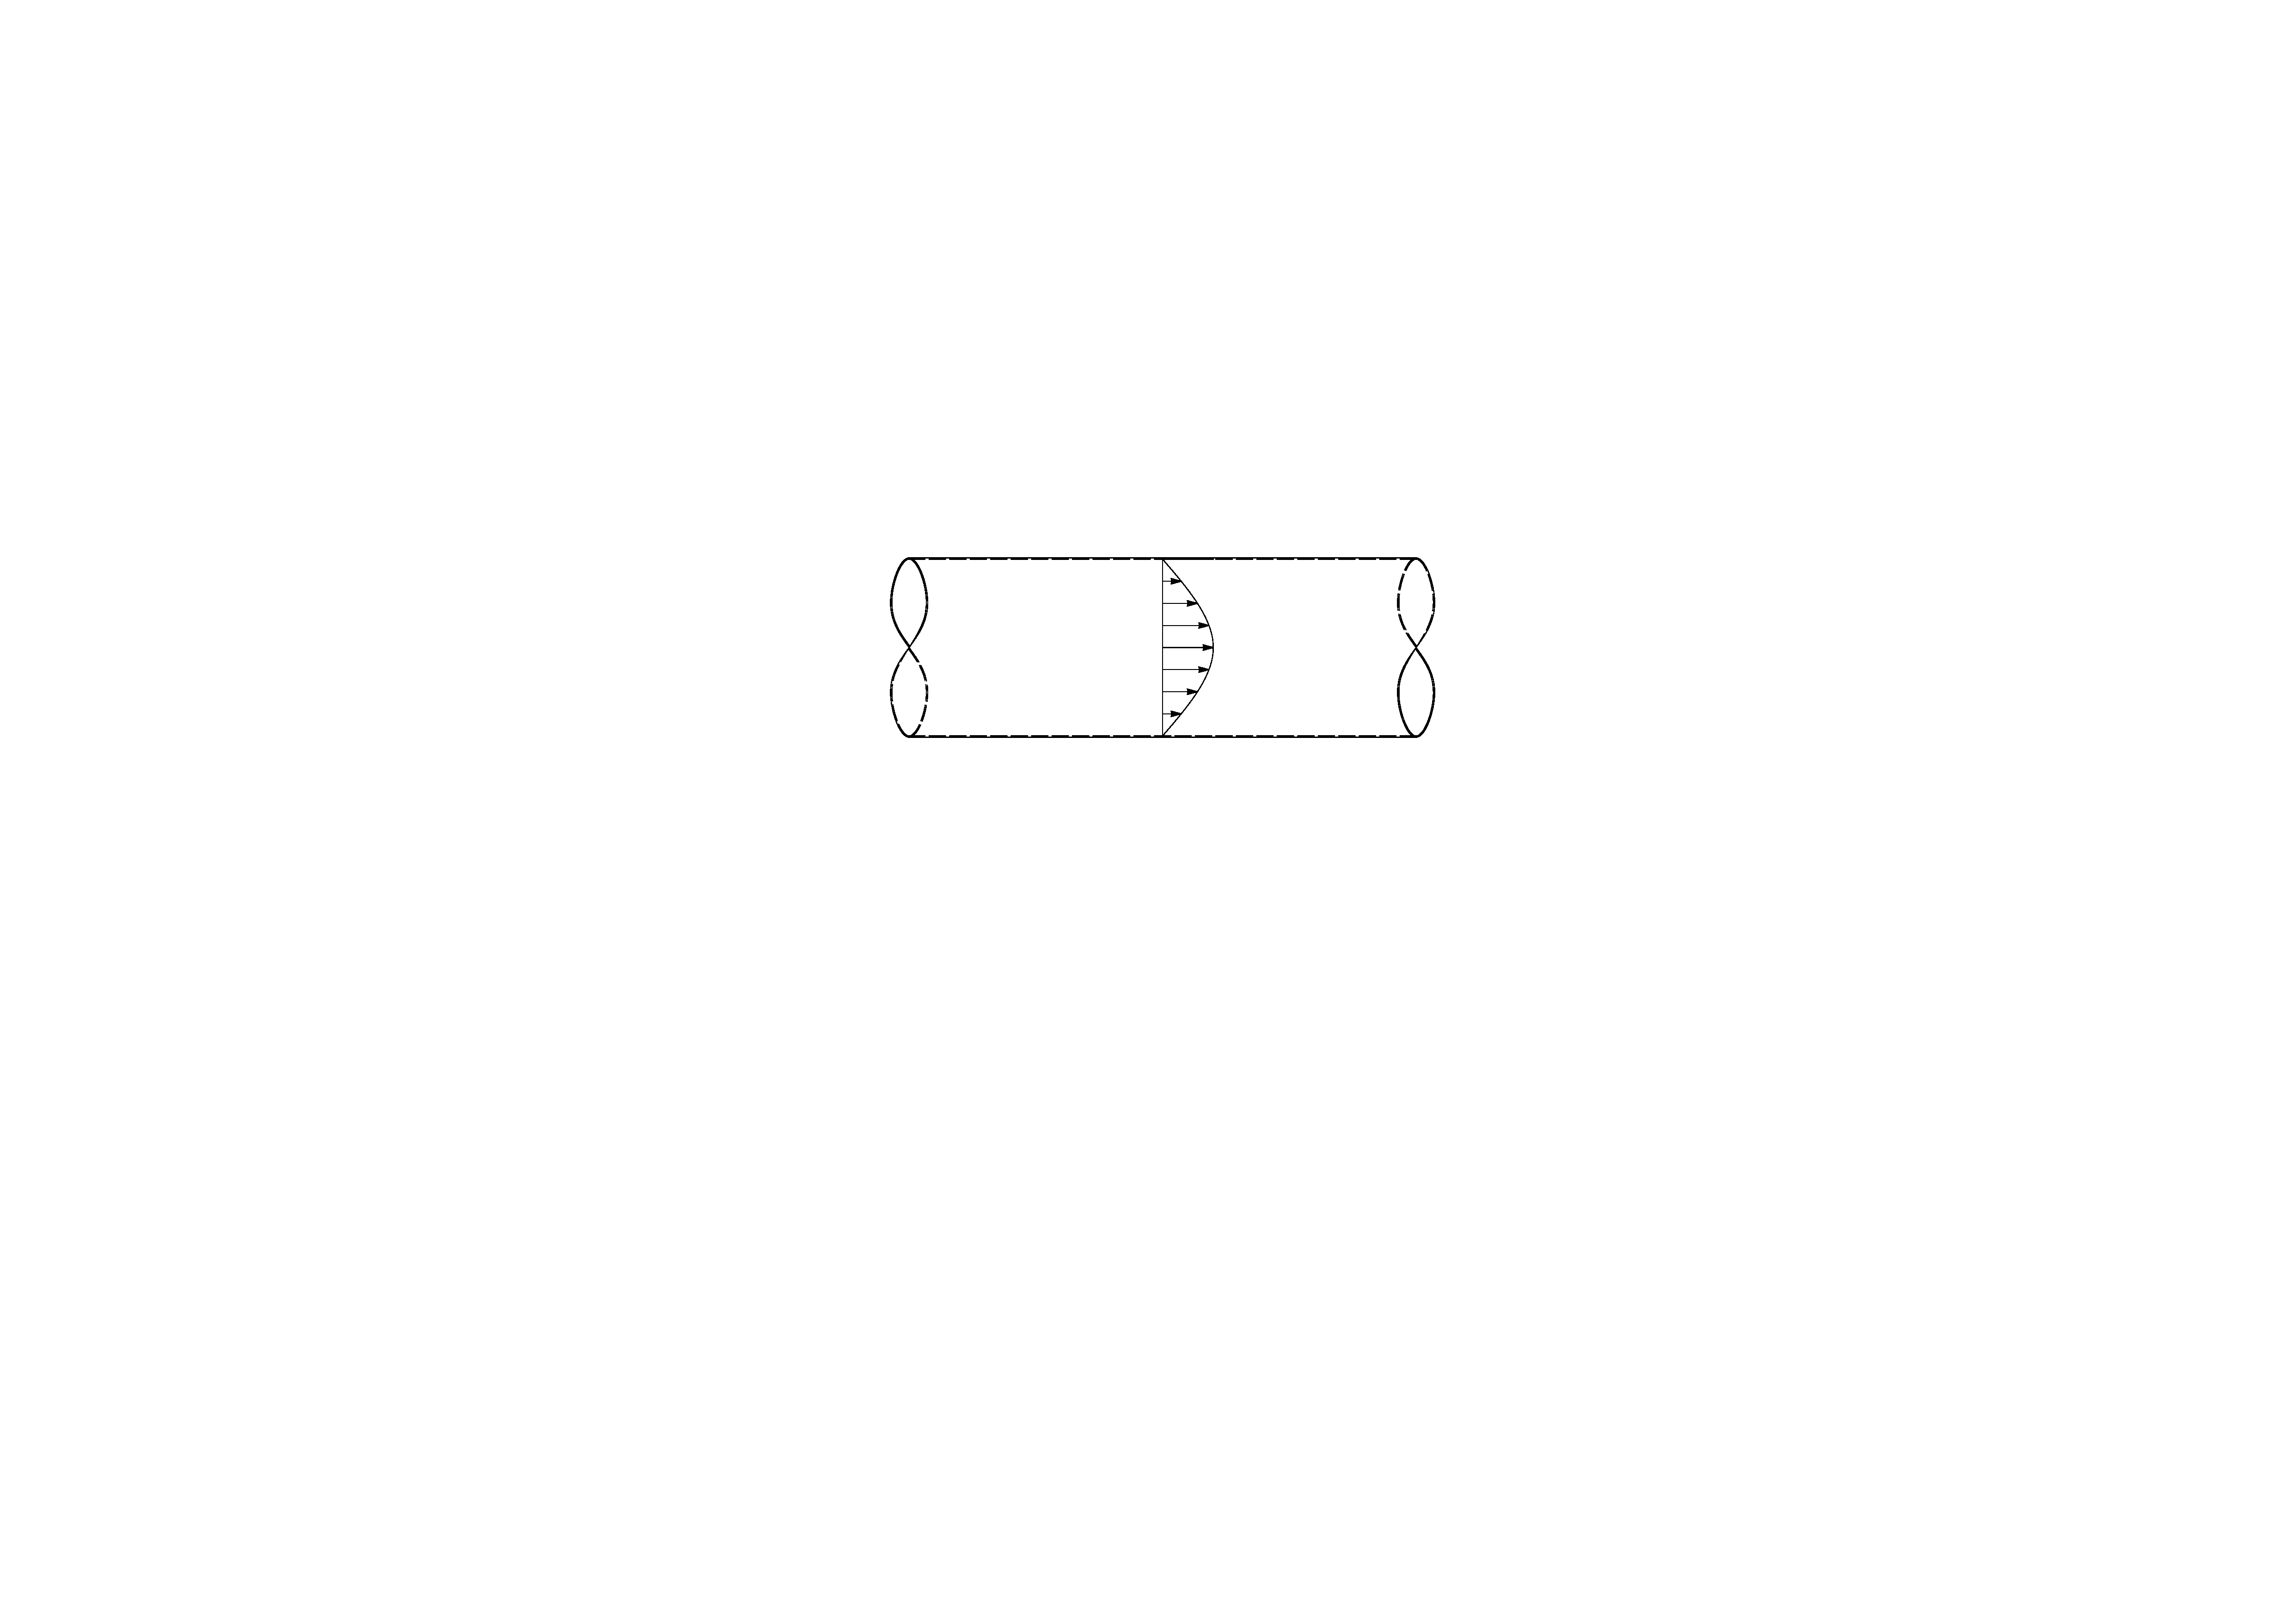
\includegraphics[width=.75\linewidth]{Figuras/EscLaminar.pdf}
        \caption{Escoamento laminar.}
        \label{fig:EscLaminar}
      \end{subfigure}
      \begin{subfigure}{.45\textwidth}
        \centering
        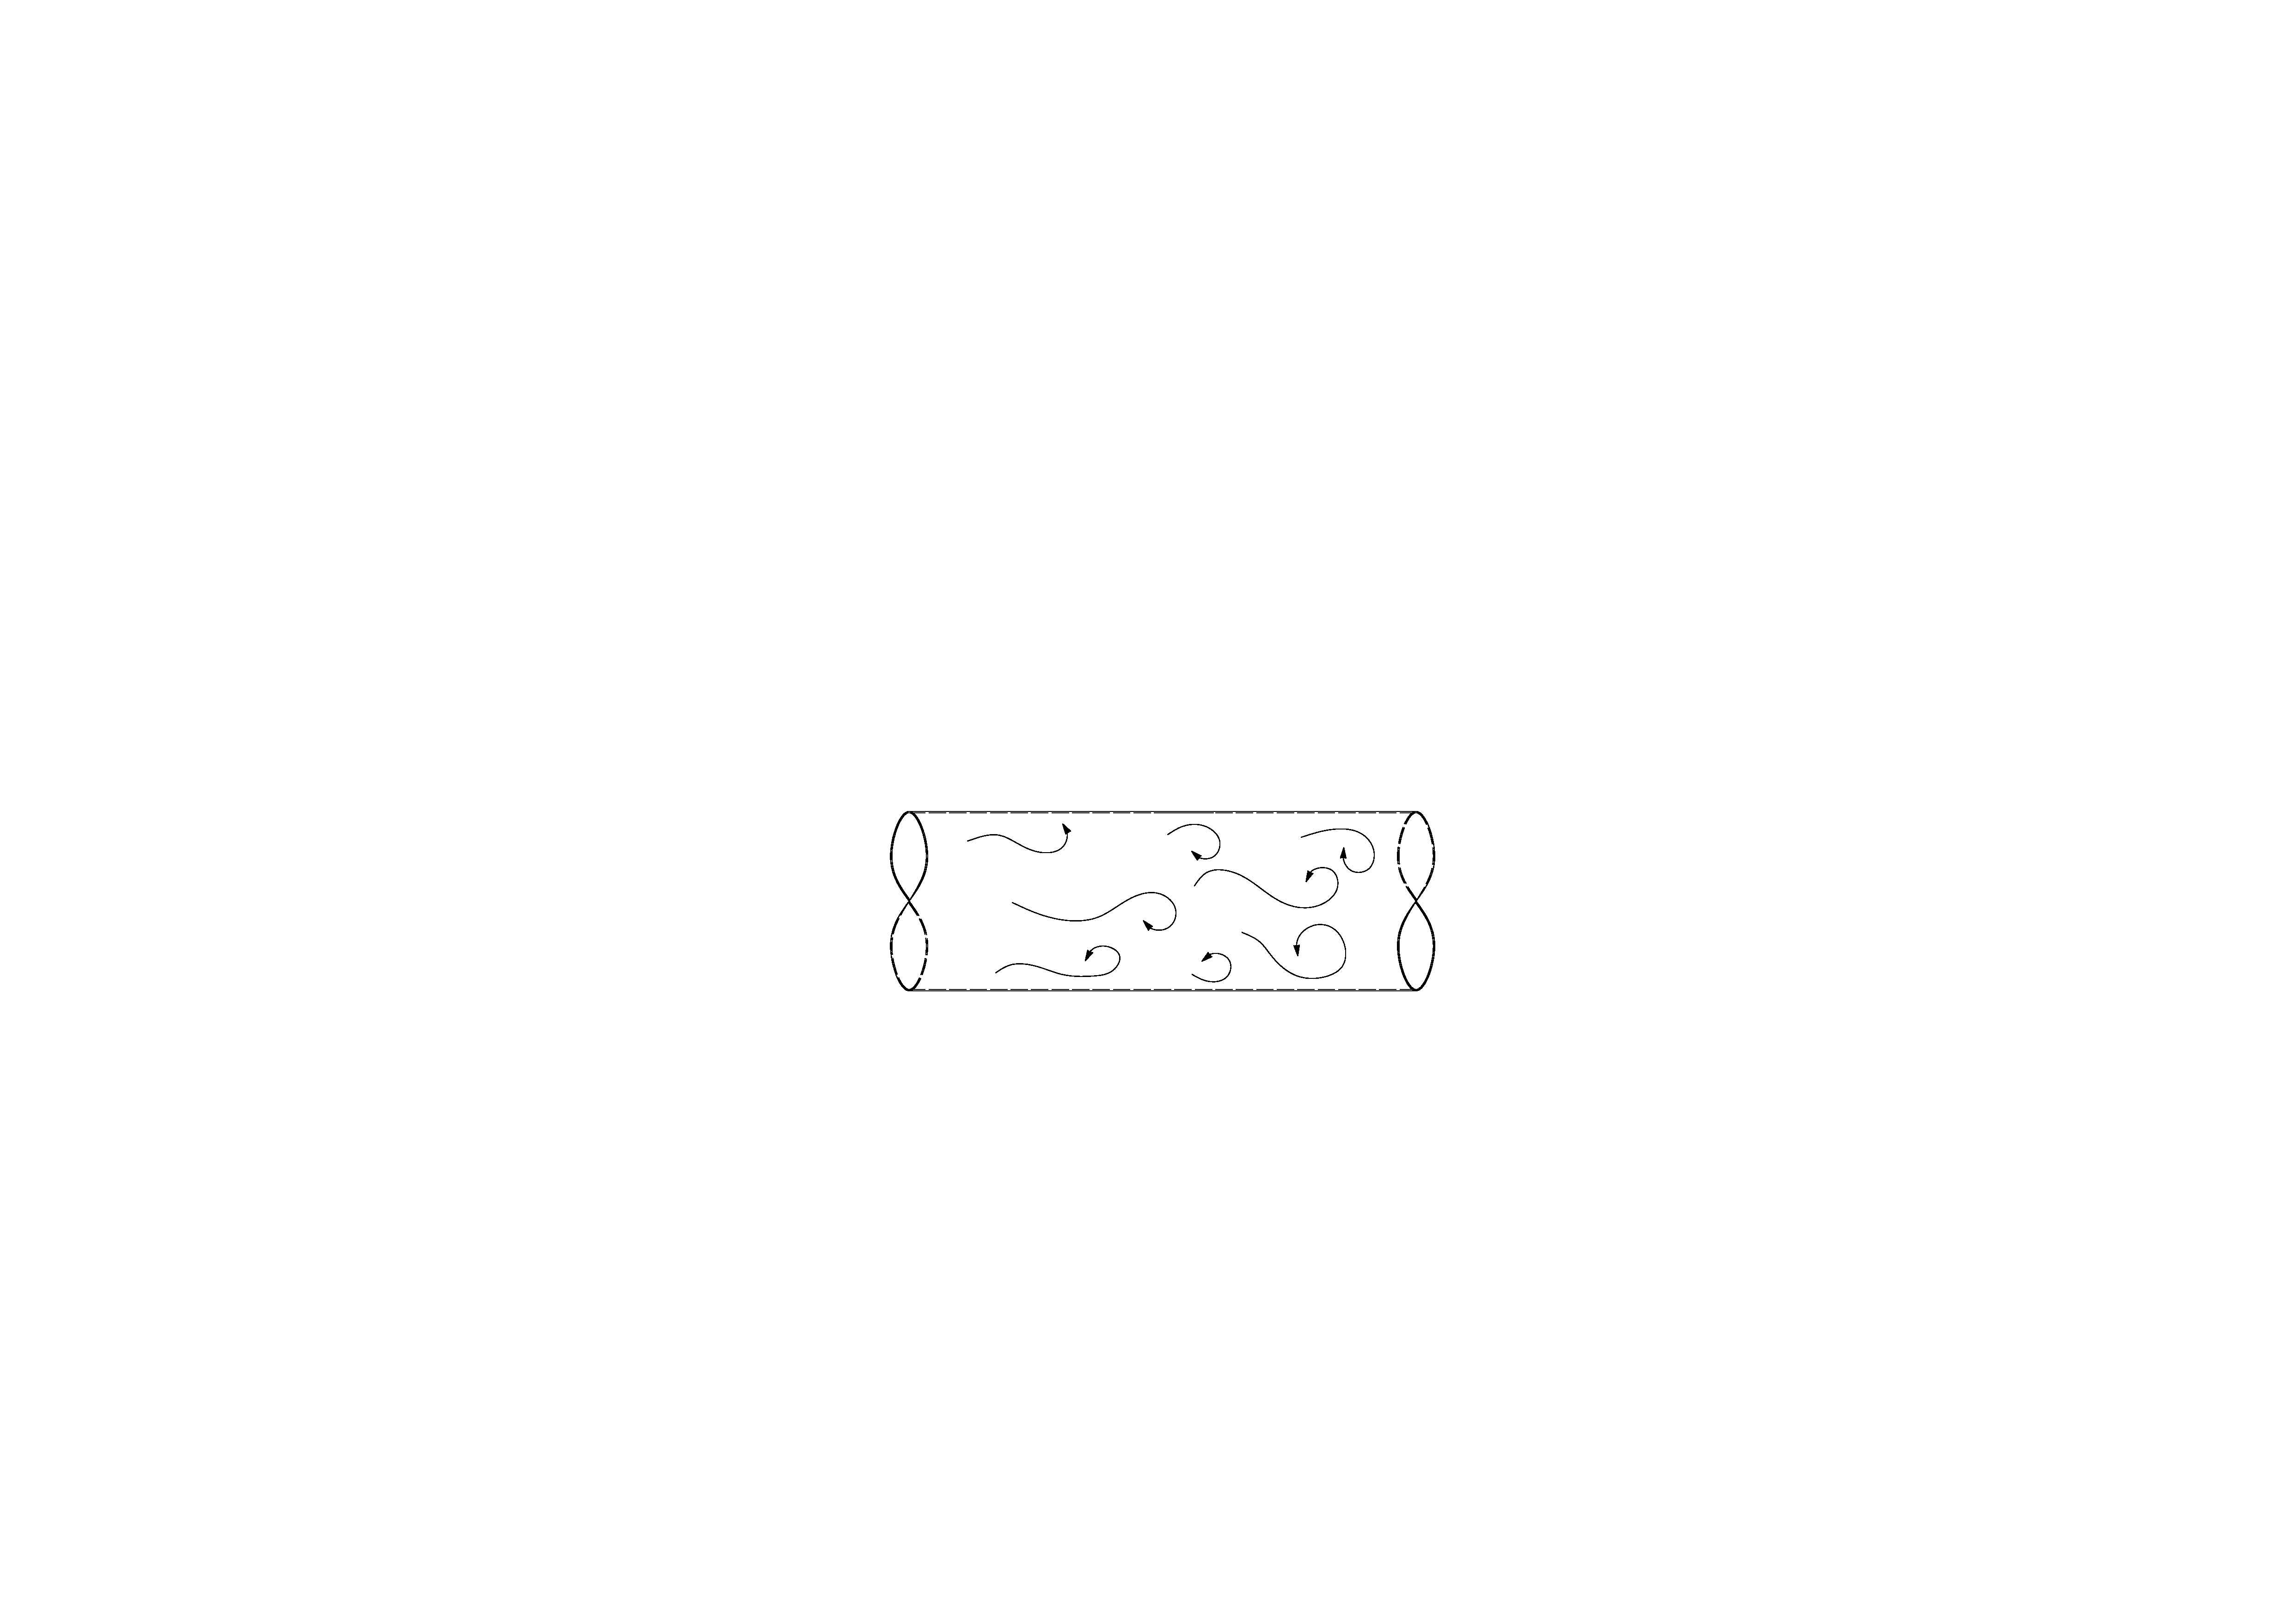
\includegraphics[width=.75\linewidth]{Figuras/EscTurbulento.pdf}
        \caption{Escoamento turbulento.}
        \label{fig:EscTurbulento}
      \end{subfigure}
    \\Fonte: Autoria Própria (\the\year).
\end{figure}

\end{document}

%==================================================================================================
\section{Objetivos}
%==================================================================================================

Esta proposta tem como objetivo principal o estudo de formulações numéricas e a implementação computacional de modo a se obter ferramentas computacionais eficientes e precisas para a simulação de problemas de interação fluido-estrutura com elevados números de Reynolds, onde possa haver efeitos de turbulência. Dentro desse escopo, alguns objetivos específicos devem ser alcançados:

\begin{itemize}
    \item Estudo das formulações estabilizadas do método dos elementos finitos para escoamentos incompressíveis com contornos móveis, com destaque para as estabilizações SUPG, LSIC, PSPG e VMS;

    \item Estudo da formulação posicional do MEF para análise dinâmica de sólidos e cascas com grandes deslocamentos;

    \item Estudo das técnicas de acoplamento particionado fluido-estrutura com malhas móveis;

    \item Estudo dos diversos modelos de turbulência no contexto do MEF;

    \item Implementação da formulação estabilizada \VMS;

    \item Implementação do modelo \LES;

    \item Acoplamento do código para mecânica dos fluidos com programa para análise não linear de estruturas de cascas;

    \item Estudo comparativo dos modelos implementados através da simulação de exemplos disponíveis na literatura.
\end{itemize}

%==================================================================================================
% METODOLOGIA
%==================================================================================================

%==================================================================================================
\chapter{Metodologia e cronograma} \label{MetodologiaCronograma}
%==================================================================================================

Tendo em vista a complexidade dos problemas em estudo, delimita-se os estudos dos problemas de interação fluido-estrutura considerando escoamento incompressível viscoso interagindo com estruturas reticuladas com grandes deslocamentos. Adota-se acoplamento particionado forte do tipo bloco-iterativo com método de malha móvel para o fluido empregando-se a descrição Lagrangiana-Euleriana Arbitrária (ALE). Essa abordagem é adotada por ser reconhecidamente robusta, modular e amplamente utilizada para análises de IFE.

Assim como os problemas a serem estudados, as implementações necessárias também são bastante complexas, sendo importante a adoção de uma metodologia de programação que aproveite os códigos disponíveis e ao mesmo tempo facilite alterações de tipos de elementos, modelos constitutivos, métodos de solução de sistemas e operações algébricas, e mais importante no contexto desta proposta, diferentes métodos de estabilização e diferentes modelos de turbulência.

Dessa forma, adota-se a linguagem de programação C++ orientada a objeto, em um sistema operacional Linux, uma vez que se é possível aproveitar diversos códigos já desenvolvidos pelo grupo de pesquisa, a saber, programa de elementos finitos para análise de escoamentos incompressíveis empregando-se elementos triangulares (2D) e tetraédricos (3D) com aproximações linear ou quadrática e programa para análise dinâmica não linear geométrica de estruturas de casca finas ou espessas empregando elementos triangulares cúbicos.

Para a solução da mecânica dos sólidos será empregado o MEF baseado em posições, aproveitando-se um programa para análise de cascas com cinemática de Reissner-Mindlin, já desenvolvido pelo grupo de pesquisa. A formulação baseada em posições emprega uma descrição Lagrangiana Total, sendo adotado o modelo constitutivo de Saint-Venant Kirchhoff  com a medida de deformação de Green-Lagrange. O elemento de casca utilizado possui 7 graus de liberdade por nó, a saber, 3 coordenadas de posição, 3 coordenadas de um vetor generalizado, inicialmente perpendicular à superfície média da casca, e 1 parâmetro de enriquecimento para permitir variação linear da deformação na direção da espessura. A aproximação das derivadas temporais do problema é feita com integrador temporal $alpha$-generalizado. O processo de solução dos sistema não linear é obtida por meio do método iterativo de Newton-Raphson. 

Já para a solução da mecânica dos fluidos fluido, parte-se de um código computacional para escoamentos bidimensionais e tridimensionais empregado a formulação estabilizada PSPG/SUPG do MEF e a descrição ALE, o que possibilita a representação de contornos móveis. Assim como no sólido, a aproximação temporal é dada pelo integrador $\alpha$-generalizado e o método de Newton-Raphson é empregado para a solução do sistema não linear. Neste código é parte desta proposta a implementação de elementos Taylor-Hood, com aproximação quadrática para velocidades e linear para pressão, a implementação da técnica de estabilização \LSIC (LSIC) para captura de vórtices, assim comoos modelos de turbulência RANS e LES e o modelo de estabilização VMS (implementações essas que já foram finalizadas).

Após o estudo e verificação isolada das ferramentas para solução do fluido e do sólido, parte-se para o acoplamento.
Para isso será adotado um modelo de acoplamento particionado forte do tipo bloco-iterativo, sendo a movimentação da malha do fluido realizada por meio de um problema fictício de elasticidade, considerando-se a malha do fluido como um sólido elástico com deslocamentos prescritos no contorno.

% \textcolor{red}{-Falar como você vai resolver o sólido (citar o programa de cascas disponível, a formulação empregada e a integração temporal adotada). Especificar se você vai implementar alguma coisa nele ou só utilizar.}

% \textcolor{red}{-Falar como você vai resolver o fluido considerando contornos móveis (citar o programa de fluido disponível, a formulação/elementos empregados e a integração temporal adotada). Especificar o que você vai implementar}

% \textcolor{red}{-Falar sobre a técnica de acoplamento a ser adotada para unir os códigos}

Será empregado o protocolo de processamento paralelo \textit{Message Passing Interface} (MPI), com utilização da biblioteca PETSc (\textit{Portable, Extensible Toolkit for Scientific Computation}) \cite{petsc-web-page}, a qual é reconhecidamente eficiente para solução de sistemas esparços que necessitem de alto desempenho computacional, tendo suporte para C++ e MPI.  As malhas serão geradas a partir do programa Gmsh \cite{geuzaine2009gmsh}, e os resultados serão interpretados graficamente por meio do visualizador Paraview \cite{ahrens2005paraview} e por meio do programa gnuPlot, no caso da geração de gráficos de linha 2D ou 3D. Nota-se que prioriza-se o uso de ferramentas computacionais livres e de código aberto para facilitar a distribuição e as atualizações da ferramenta computacional resultante.

%==================================================================================================
\section{Cronograma}
%==================================================================================================

% \textcolor{red}{As atividades estavam insuficientes para descrever o seu trabalho durante o curso (pode incluir as disciplinas, já que o cronograma é do trabalho de mestrado como todo). Adicionei outras atividades, verifique se não falta nada e atualize o cronograma (Pode incluir o exame de qualificação...).}

As atividades necessárias para se alcançar os objetivos desta pesquisa são organizadas da seguinte maneira:

\begin{enumerate}[label=\alph*.]
	\item\label{M:1} Cursar disciplinas do programa de mestrado;
	\item\label{M:2} Revisão bibliográfica a ser realizada de forma contínua ao longo de todo o trabalho, para que o mesmo se mantenha atualizado frente ao estado da arte durante toda sua execução;
	\item\label{M:3} Estudo das formulações estabilizadas do método dos elementos finitos para a solução de escoamentos incompressíveis com contornos móveis;
	\item\label{M:4} Estudo dos modelos de turbulência RANS e LES;
	\item\label{M:5} Estudo do código computacional para escoamentos incompressíveis disponível e implementações do modelo de estabilização VMS;
	\item\label{M:6} Implementação computacional dos modelos de turbulência no código de escoamentos incompressíveis;
	\item\label{M:7} Verificação dos modelos de turbulência implementados no contexto de escoamentos com contornos fixos a partir de exemplos presentes na literatura;
	\item\label{M:8} Estudo da formulação posicional do MEF para elementos de casca com cinemática de Reissner-Mindlin;
	\item\label{M:9} Exame de qualificação de mestrado;
	\item\label{M:10} Estudo e implementação do modelo de acoplamento particionado do tipo bloco-iterativo;
	\item\label{M:11} Verificação e Estudo dos modelos implementados no contexto dos problemas de iteração fluido-estrutura com elevados números de Reynolds;
	\item\label{M:12} Redação da dissertação e elaboração de artigos para revistas;
	\item \label{M:13} Defesa do mestrado.
\end{enumerate}

Essas atividades são organizadas cronologicamente, ao longo do tempo disponível para a conclusão do mestrado, de acordo com o cronograma da Tabela \ref{Cronograma}.

\definecolor{lightgray}{RGB}{153,153,153}
\definecolor{lightblue}{RGB}{126,194,216}

\begin{table}[h!]
	\caption{Cronograma de atividades}
	\fontsize{8}{14}\selectfont
	\centering
	\newcommand{\Rx}{\cellcolor{lightblue}}
	\newcommand{\Px}{\cellcolor{lightgray}}
	\begin{tabular}{|c|ccccccccc|cccccccccccc|cccc|}
		\hline
		\MR{2}{*}{Item} & \MC{9}{c|}{2022} & \MC{12}{c|}{2023} & \MC{4}{c|}{2024}                                                                                                                                     \\ \cline{2-26}
		                & A                & M                 & J                & J   & A   & S   & O   & N   & D   & J   & F   & M   & A   & M   & J   & J   & A   & S   & O   & N   & D   & J   & F   & M   & A   \\ \hline
		\ref{M:1}       & \Rx              & \Rx               & \Rx              & \Rx & \Rx & \Rx & \Rx & \Rx & \Rx &     &     &     &     &     &     &     &     &     &     &     &     &     &     &     &     \\ \hline
		\ref{M:2}       & \Rx              & \Rx               & \Rx              & \Rx & \Rx & \Rx & \Rx & \Rx & \Rx & \Rx & \Rx & \Rx & \Rx & \Rx & \Rx & \Rx & \Px & \Px & \Px & \Px & \Px & \Px & \Px & \Px &     \\ \hline
		\ref{M:3}       &                  &                   &                  &     & \Rx & \Rx & \Rx & \Rx & \Rx & \Rx & \Rx &     &     &     &     &     &     &     &     &     &     &     &     &     &     \\ \hline
		\ref{M:4}       &                  &                   &                  &     &     &     &     & \Rx & \Rx & \Rx & \Rx & \Rx & \Rx & \Rx &     &     &     &     &     &     &     &     &     &     &     \\ \hline
		\ref{M:5}       &                  &                   &                  &     &     &     &     &     &     &     & \Rx & \Rx & \Rx & \Rx &     &     &     &     &     &     &     &     &     &     &     \\ \hline
		\ref{M:6}       &                  &                   &                  &     &     &     &     &     &     &     &     &     &     & \Rx & \Rx & \Rx & \Px & \Px & \Px &     &     &     &     &     &     \\ \hline
		\ref{M:7}       &                  &                   &                  &     &     &     &     &     &     &     &     &     &     &     & \Rx & \Rx &     &     &     &     &     &     &     &     &     \\ \hline
		\ref{M:8}       &                  &                   &                  &     &     &     &     &     &     &     &     &     &     & \Rx & \Rx & \Rx &     &     &     &     &     &     &     &     &     \\ \hline
		\ref{M:9}       &                  &                   &                  &     &     &     &     &     &     &     &     &     &     &     &     &     & \Px &     &     &     &     &     &     &     &     \\ \hline
		\ref{M:10}      &                  &                   &                  &     &     &     &     &     &     &     &     &     &     &     &     &     & \Px & \Px & \Px & \Px &     &     &     &     &     \\ \hline
		\ref{M:11}      &                  &                   &                  &     &     &     &     &     &     &     &     &     &     &     &     &     &     &     &     & \Px & \Px & \Px & \Px &     &     \\ \hline
		\ref{M:12}      & \Rx              & \Rx               & \Rx              & \Rx & \Rx & \Rx & \Rx & \Rx & \Rx & \Rx & \Rx & \Rx & \Rx & \Rx & \Rx & \Rx & \Px & \Px & \Px & \Px & \Px & \Px & \Px & \Px &     \\ \hline
		\ref{M:13}      &                  &                   &                  &     &     &     &     &     &     &     &     &     &     &     &     &     &     &     &     &     &     &     &     &     & \Px \\ \hline
	\end{tabular}
	\label{Cronograma}
\end{table}

\begin{minipage}{\textwidth}
	\fontsize{8}{14}\selectfont
	\centering
	\colorbox{lightblue}{\rule{0pt}{10pt}\rule{10pt}{0pt}} Já realizado \quad
	\colorbox{lightgray}{\rule{0pt}{10pt}\rule{10pt}{0pt}} Pendente \quad
\end{minipage}

%==================================================================================================
\section{Justificativa}
%==================================================================================================

Os avanços na área da engenharia colocam em evidência a necessidade cada vez maior de se determinar de forma precisa as variáveis necessárias ao dimensionamento de estruturas, sejam referentes à resistência dos materiais utilizados, ou às solicitações atuantes. Nesse sentido, em diversas ocasiões, os efeitos advindos da interação fluido-estrutura (IFE) são responsáveis por submeter estruturas a esforços consideráveis, o que demanda que esses efeitos sejam adequadamente estudados. Assim, mesmo que diversos trabalhos tenham sido realizados, resultando em grandes avanços na área, alguns desafios se mantêm, como o elevado custo computacional relacionado à simulações de IFE, o que demanda muito tempo pra a obtenção de resultados, inviabilizando sua aplicação em muitos projetos usuais de engenharia.

Outro desafio que se pode destacar é referente aos problemas de acoplamento, uma vez que os modelos constitutivos que regem tanto os sólidos quanto os fluidos são distintos, assim como as variáveis empregadas para descrever o comportamento de cada um. Também verifica-se que o sistema de equações fundamental para o estudo desses problemas, ou não possui solução analítica, ou essa só pode ser obtida para casos simples e com hipóteses bastante simplificadoras, sem muita possibilidade de generalizações.

Dessa forma, os métodos numéricos são vistos como uma alternativa necessária. Dentre os métodos empregados, pode-se destacar o dos Elementos Finitos (MEF), com aplicações tanto para modelar o sólido como para o fluido. Esse método ganha atenção, uma vez que pode se adequar com certa facilidade à problemas de geometria complexa, garantindo ainda facilidade para aplicação de condições de contorno.

Embora no contexto da mecânica dos fluidos, a utilização do MEF segundo o método de Bubnov-Galerkin possa gerar oscilações espúrias, decorrentes dos termos convectivos, de ondas de choque nos casos compressíveis, ou da interpolação da pressão por espaços de funções inadequados nos casos incompressíveis, todos esses problemas já dispõem de técnicas consistentes para que sejam evitados. Como exemplos, destacam-se a técnica SUPG para estabilização da convecção, a técnica PSPG ou o uso de elementos Taylor-Hood para estabilização da pressão nos escoamentos incompressíveis e a introdução de operadores de captura de choque para os casos compressíveis.

Outra questão envolvendo a utilização do MEF nesse tipo de problema está relacionado ao custo computacional, que também se mostra como um desafio enfrentado por pesquisadores dessa área. Nesse cenário, problemas de escoamento turbulentos se tornam ainda mais custosos, devido à alguns fenômenos como a manifestação de vórtices, geralmente tridimensionais, de forma desordenada, instável e em uma grande amplitude de escalas. Assim necessita-se de malhas muito refinadas para capturar a ocorrência dessas estruturas. Para que a simulação desses problemas seja estável em qualquer nível de discretização, e possa resultar em respostas consistentes a custos computacionais aceitáveis, faz-se necessária a adoção de modelos de turbulência, como  aqueles baseados na decomposição de Reynolds (RANS) ou em grandes vórtices (LES), ou de técnicas multiescala adequadas.

Sendo assim, o presente trabalho é justificado ao propor o desenvolvimento de uma ferramenta computacional eficiente e precisa, aplicada a problemas de IFE com escoamentos turbulentos com a opção de se aplicar modelo de turbulência. Igualmente, fica justificado a proposta de estudar e comparar os diferentes modelos e estabilizações a serem implementadas quando da aplicação a problemas de IFE. A presente pesquisa visa ainda aprimorar as ferramentas computacionais que estão sendo desenvolvidas pelo grupo de pesquisa do SET, ampliando seu leque de aplicações.
% % Introdução

\documentclass[_ArquivoPrincipal.tex]{subfiles}

\begin{document}

%==================================================================================================
\chapter{Estado Da Arte}
%==================================================================================================
	
No presente capítulo serão abordados os principais temas relacionados à problemas de Interação Fluido-Estrutura (IFE), tendo como ênfase os modos de turbulência. Serão destacados os principais métodos de cálculos envolvendo a dinâmica das estruturas computacional (\ref{CSD}), a dinâmica dos fluidos computacional (\ref{CFD}) e alguns modelos de turbulências (\ref{MT}).

%==================================================================================================
\section{Dinâmica Das Estruturas Computacional} \label{CSD}
%==================================================================================================

A mecânica dos sólidos visa a determinação de parâmetros referentes à elementos estruturais sujeitos a solicitações externas, tais como tensões e deformações, ou forças e deslocamentos de determinados pontos dos mesmos. Para isso são desenvolvidos diversos métodos com a finalidade de melhor descrever o comportamento das estruturas, como o Método dos Elementos Finitos (MEF), que se apresenta como a ferramenta computacional mais amplamente utilizada para esse fim.

Nesse sentido vale ressaltar os trabalhos de \citeonline{hughes1981nonlinear, argyris1982excursion, ibrahimbegovic2002role, pimenta2004fully, battini2006choice} e \citeonline{pimenta2008exact}, que realizaram análises através do MEF Corrotacional, que se trata de uma formulação onde os deslocamentos e rotações dos elementos são os parâmetros principais da análise.

No entanto a utilização de uma análise que considera tais parâmetros nodais só se mostra eficiente ao se estudar estruturas que desenvolvem pequenos deslocamentos e deformações. Isso deve-se ao fato de essa abordagem utilizar rotações finitas como parâmetros nodais, o que pode gerar controversas em problemas envolvendo grandes rotações, uma vez que não há comutatividade entre essas grandezas. Ainda observa-se que a avaliação dinâmica de estruturas reticuladas se torna problemática, do ponto de vista da conservação de energia, além da matriz de massa ser variável, tornando o processo de integração temporal muito complexo \cite{sanches2013unconstrained}.

Com isso, vale ressaltar os trabalhos de \citeonline{coda2004simple, coda2007alternative, coda2010improved, coda2009two, coda2009unconstrained} e \citeonline{carrazedo2010alternative} que utilizam de forma bem-sucedida o MEF Posicional para análise de estruturas reticuladas e de cascas aplicadas à grandes deslocamentos. Este método se diferencia dos demais ao considerar as posições nodais, obtidas a partir de vetores indeformados, como parâmetros de análise, facilitando o cálculo de efeitos de não-linearidade geométrica.

\citeonline{sanches2013unconstrained} apresentaram uma aplicação do método dos elementos finitos posicional em elementos de cascas e constataram a presença de uma matriz de massa constante, o que possibilita a utilização de métodos de integração temporal, como o método de Newmark $\beta$, conservando, assim, o momento linear e angular em análises dinâmicas. Além disso, esse trabalho também analisou problemas envolvendo IFE, obtendo resultados favoráveis, indicando a boa aplicação desse método em problemas dessa natureza.

No âmbito da IFE, destaca-se a necessidade dessa consideração, uma vez que são observadas aplicações como, por exemplo, grandes amplitudes de deslocamentos, como \textit{flutter}, aplicações biomecânicas, estruturas infláveis \cite{karagiozis2011computational}, simulações de turbinas \cite{bazilevs20113d}, dentre outras.

%==================================================================================================
\section{Dinâmica Dos Fluidos Computacional} \label{CFD}
%==================================================================================================

Ao contrário de problemas envolvendo elementos sólidos, que possuem um estado inicial bem definido, os fluidos, em especial os Newtonianos, não o possuem, uma vez que não incapazes de resistir à tensões desviadoras, deformando-se, assim, indefinidamente quando sujeitos à essas tensões. Dessa forma, torna-se apropriada a utilização de uma descrição Euleriana para descrever os fluidos, em que os parâmetros nodais são principalmente as velocidades do mesmo \cite{fernandes2020tecnica}.

Em geral, problemas envolvendo Dinâmica dos Sólidos (\textit{Computational Solid Dynamics} - CSD) partem do princípio da estacionariedade de energias, buscando a determinação do ponto em que a energia do sistema seja mínima. Esses métodos apresentam a particularidade de surgir um sistema de equações com uma matriz simétrica e, em alguns casos, de vetores cujas componentes possuem significado físico. Porém, em problemas que envolvem a Dinâmica dos Fluidos (\textit{Computational Fluid Dynamics} - CFD), o sistema de equações possui uma matriz, na maioria dos casos, assimétrica, devido à presença de termos convectivos nas equações governantes \cite{bazilevs2013computational,brooks1982streamline}.

Nesse sentido, são desenvolvidos novos métodos, em busca de uma solução mais representativa com uma malha menos refinada. Dentre os principais desenvolvidos, vale mencionar o \textit{Streamline-Upwind/Petrov-Galerkin} (SUPG) \cite{brooks1982streamline}, \textit{Galerkin Least-Squares} (GLS) \cite{hughes1989new,tezduyar1991stabilized}, \textit{Subgrid Scales} (SGS) e \cite{hughes1995multiscale}.

Um campo que vale destacar na CFD é o que estuda os fenômenos de turbulência, uma vez que esses fenômenos podem se apresentar nas mais variadas escalas, sendo necessário a geração de uma malha muito refinada para detectar a formação dos vórtices, o que ocasiona um aumento radical no custo computacional da análise. Assim, são desenvolvidas novas técnicas afim de se obter melhores resultados, sem que haja um grande aumento no volume de cálculos. Dentre esses métodos destacam-se os métodos multiescala (\textit{Variational Multi-Scale} - VMS), as simulações de grandes vórtices (\textit{Large Eddy Simulation} - LES) \cite{hughes1995multiscale,hughes1998variational,hughes2002variational,bazilevs2010large,vsekutkovski2021partitioned}, aproximações de \textit{Reynolds-Averaged Navier-Stokes} \cite{alfonsi2009reynolds} e os métodos de atualização de malha \cite{de1993petrov}. O capítulo \ref{FT} descreve de forma mais detalhada cada um desses métodos.

%==================================================================================================
\section{Interação Fluido-Estrutura} \label{IFE}
%==================================================================================================

\textcolor{red}{TEXTO}

%==================================================================================================
\section{Modelo De Turbulência} \label{MT}
%==================================================================================================

Um fluido pode apresentar um escoamento de duas formas distintas, a depender do número de Reynolds que este apresenta (conforme ilustrado na Figura \ref{fig:Escoamentos}). Em casos cujo número de Reynolds é baixo, o escoamento é considerado laminar, ou seja, o escoamento se dá de forma semelhante ao movimento de lâminas independentes, não havendo mistura macroscópica entre as mesmas. Esse tipo de escoamento possui soluções muito mais simples de se obter, no entanto representam uma ocorrência baixa na maioria dos problemas observados na natureza. Já em casos cujo número de Reynolds é muito elevado, o escoamento é considerado turbulento. Nesse cenário há a formação de vórtices sobre o escoamento, que podem ocorrer de forma instável, desordenada e em várias escalas diferentes \cite{popiolek2005analise,shaughnessy2005introduction}. Esse fenômeno pode ser descrito de acordo com as equações de Navier-Stokes, no entanto sua resolução se apresenta com um alto grau de complexidade, uma vez que possui termos não lineares em sua composição. Assim são necessárias técnicas de solução, para que se possa obter uma solução de forma aproximada à essas equações.

\begin{figure}[h]
    \centering
    \caption{Esquema de escoamentos.\label{fig:Escoamentos}}
    \begin{subfigure}{.45\textwidth}
        \centering
        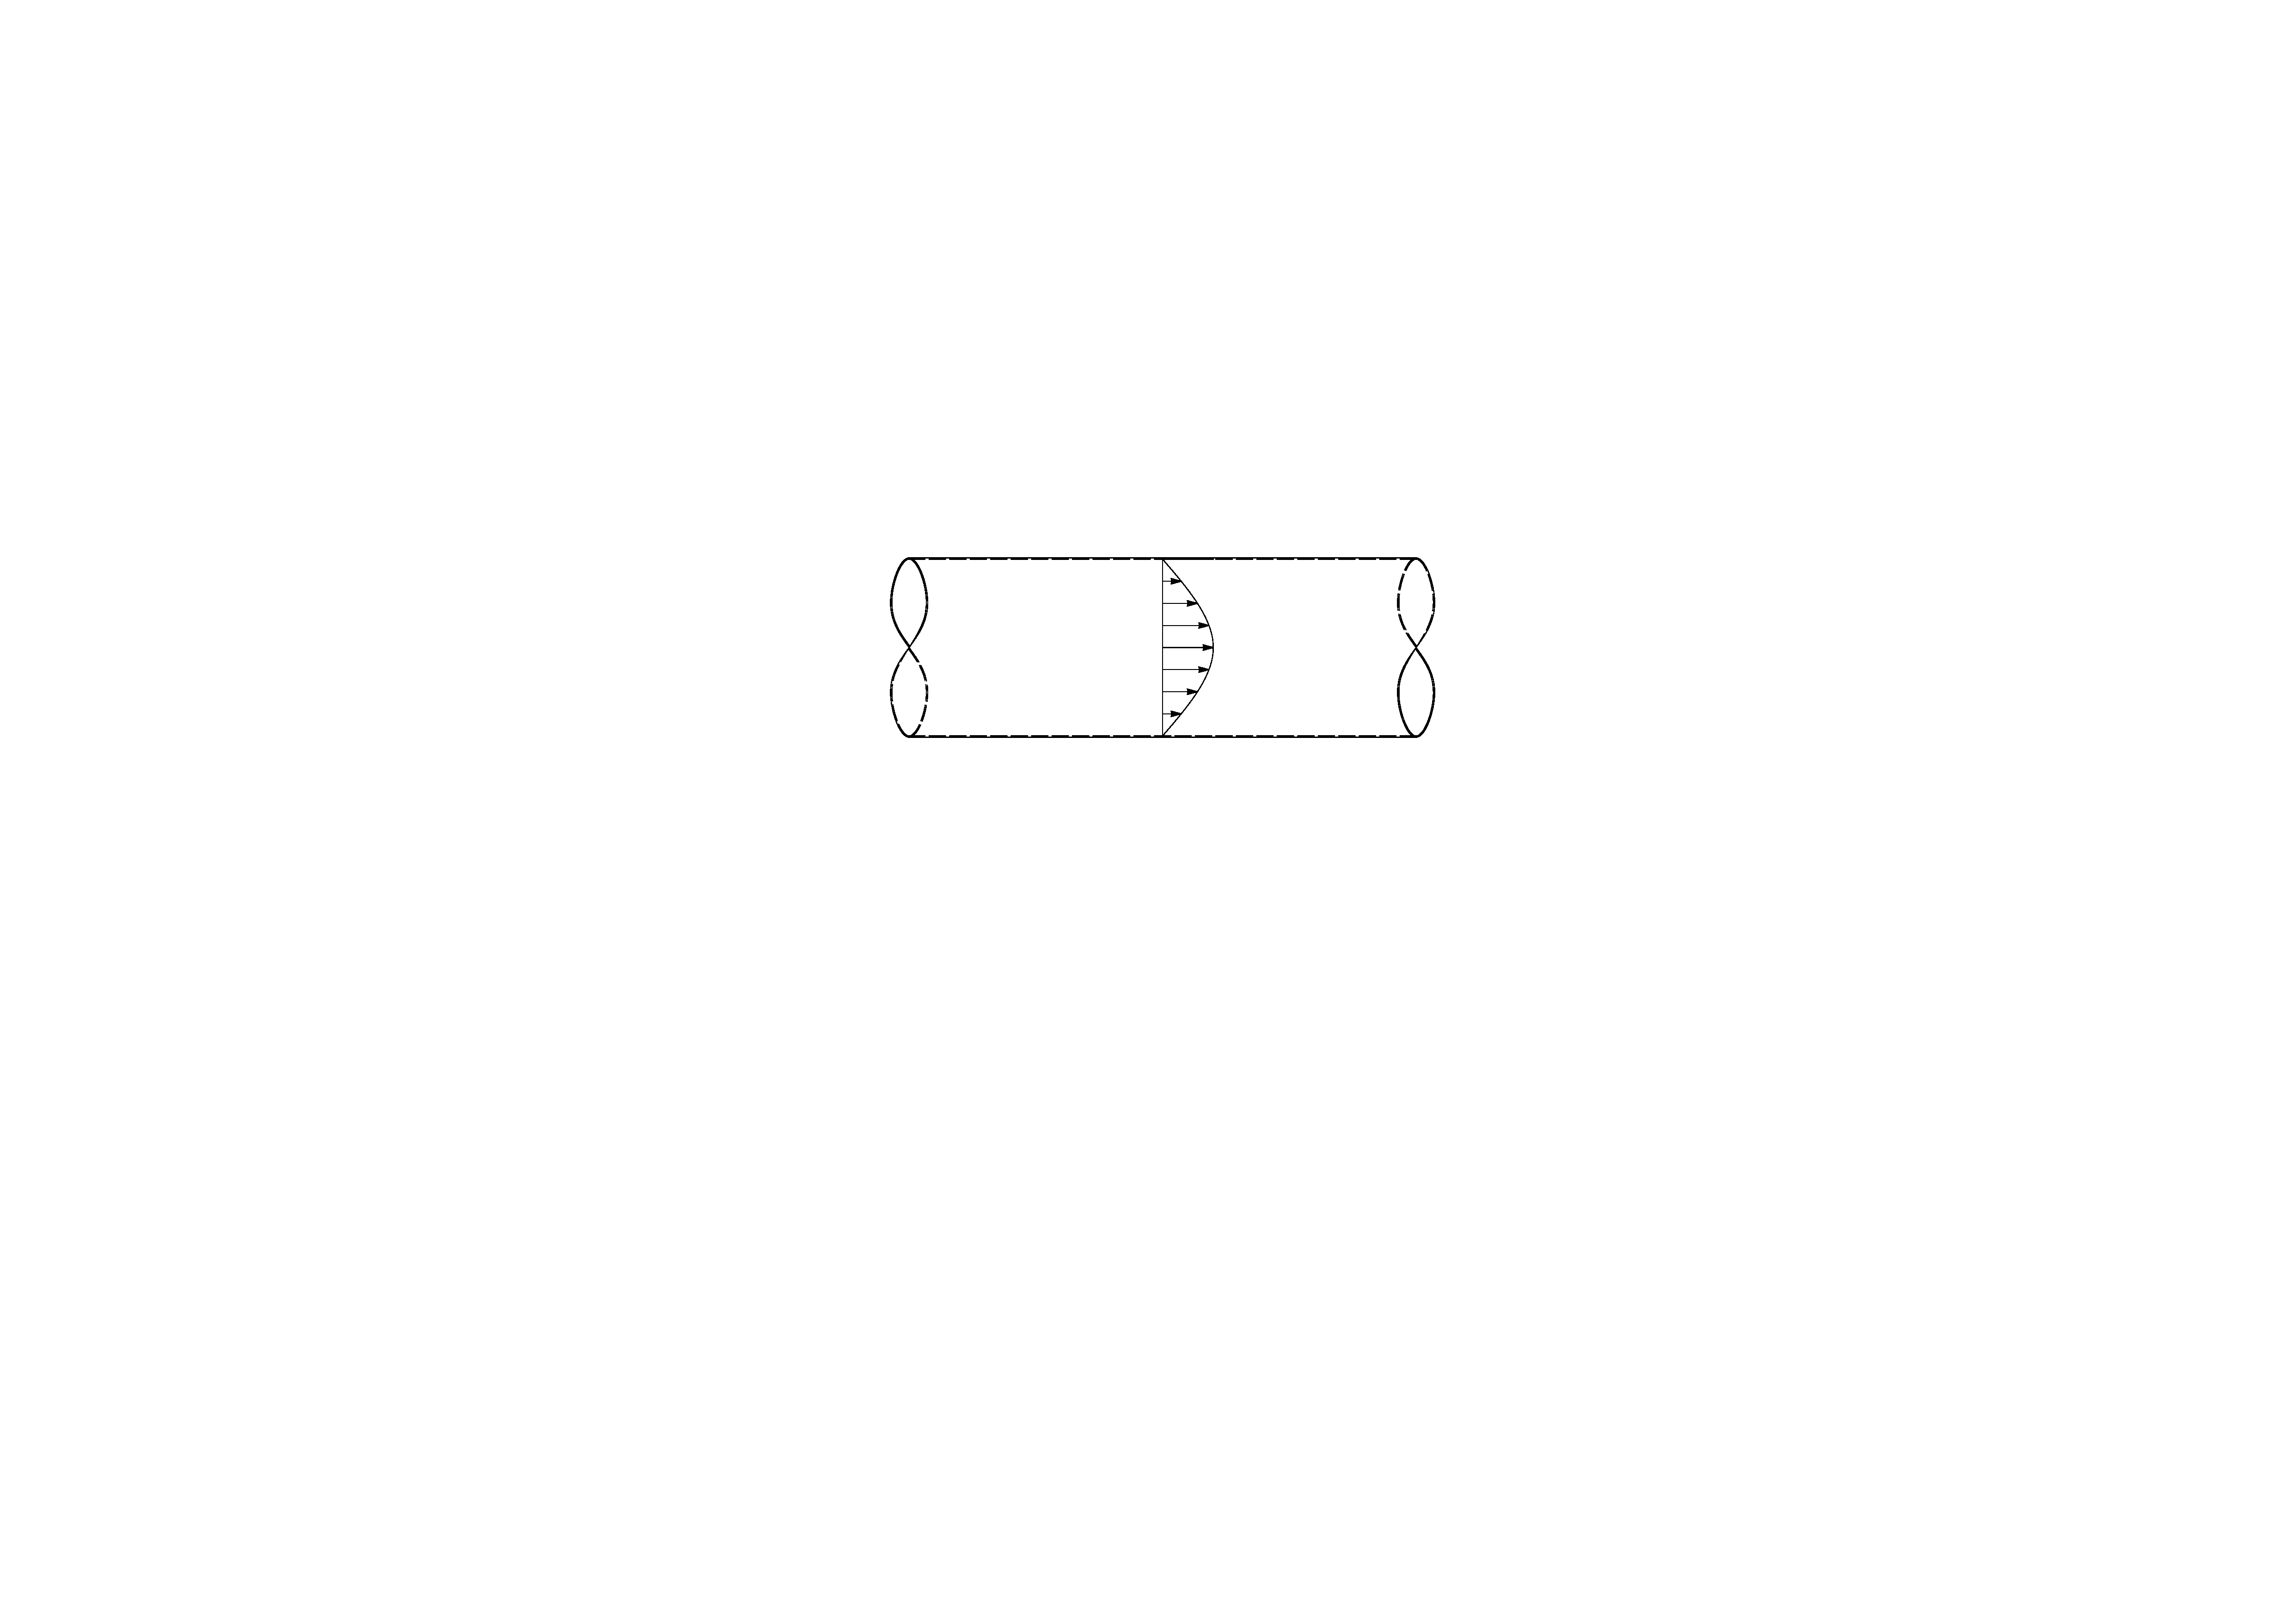
\includegraphics[width=.75\linewidth]{Figuras/EscLaminar.pdf}
        \caption{Escoamento laminar.}
        \label{fig:EscLaminar}
      \end{subfigure}
      \begin{subfigure}{.45\textwidth}
        \centering
        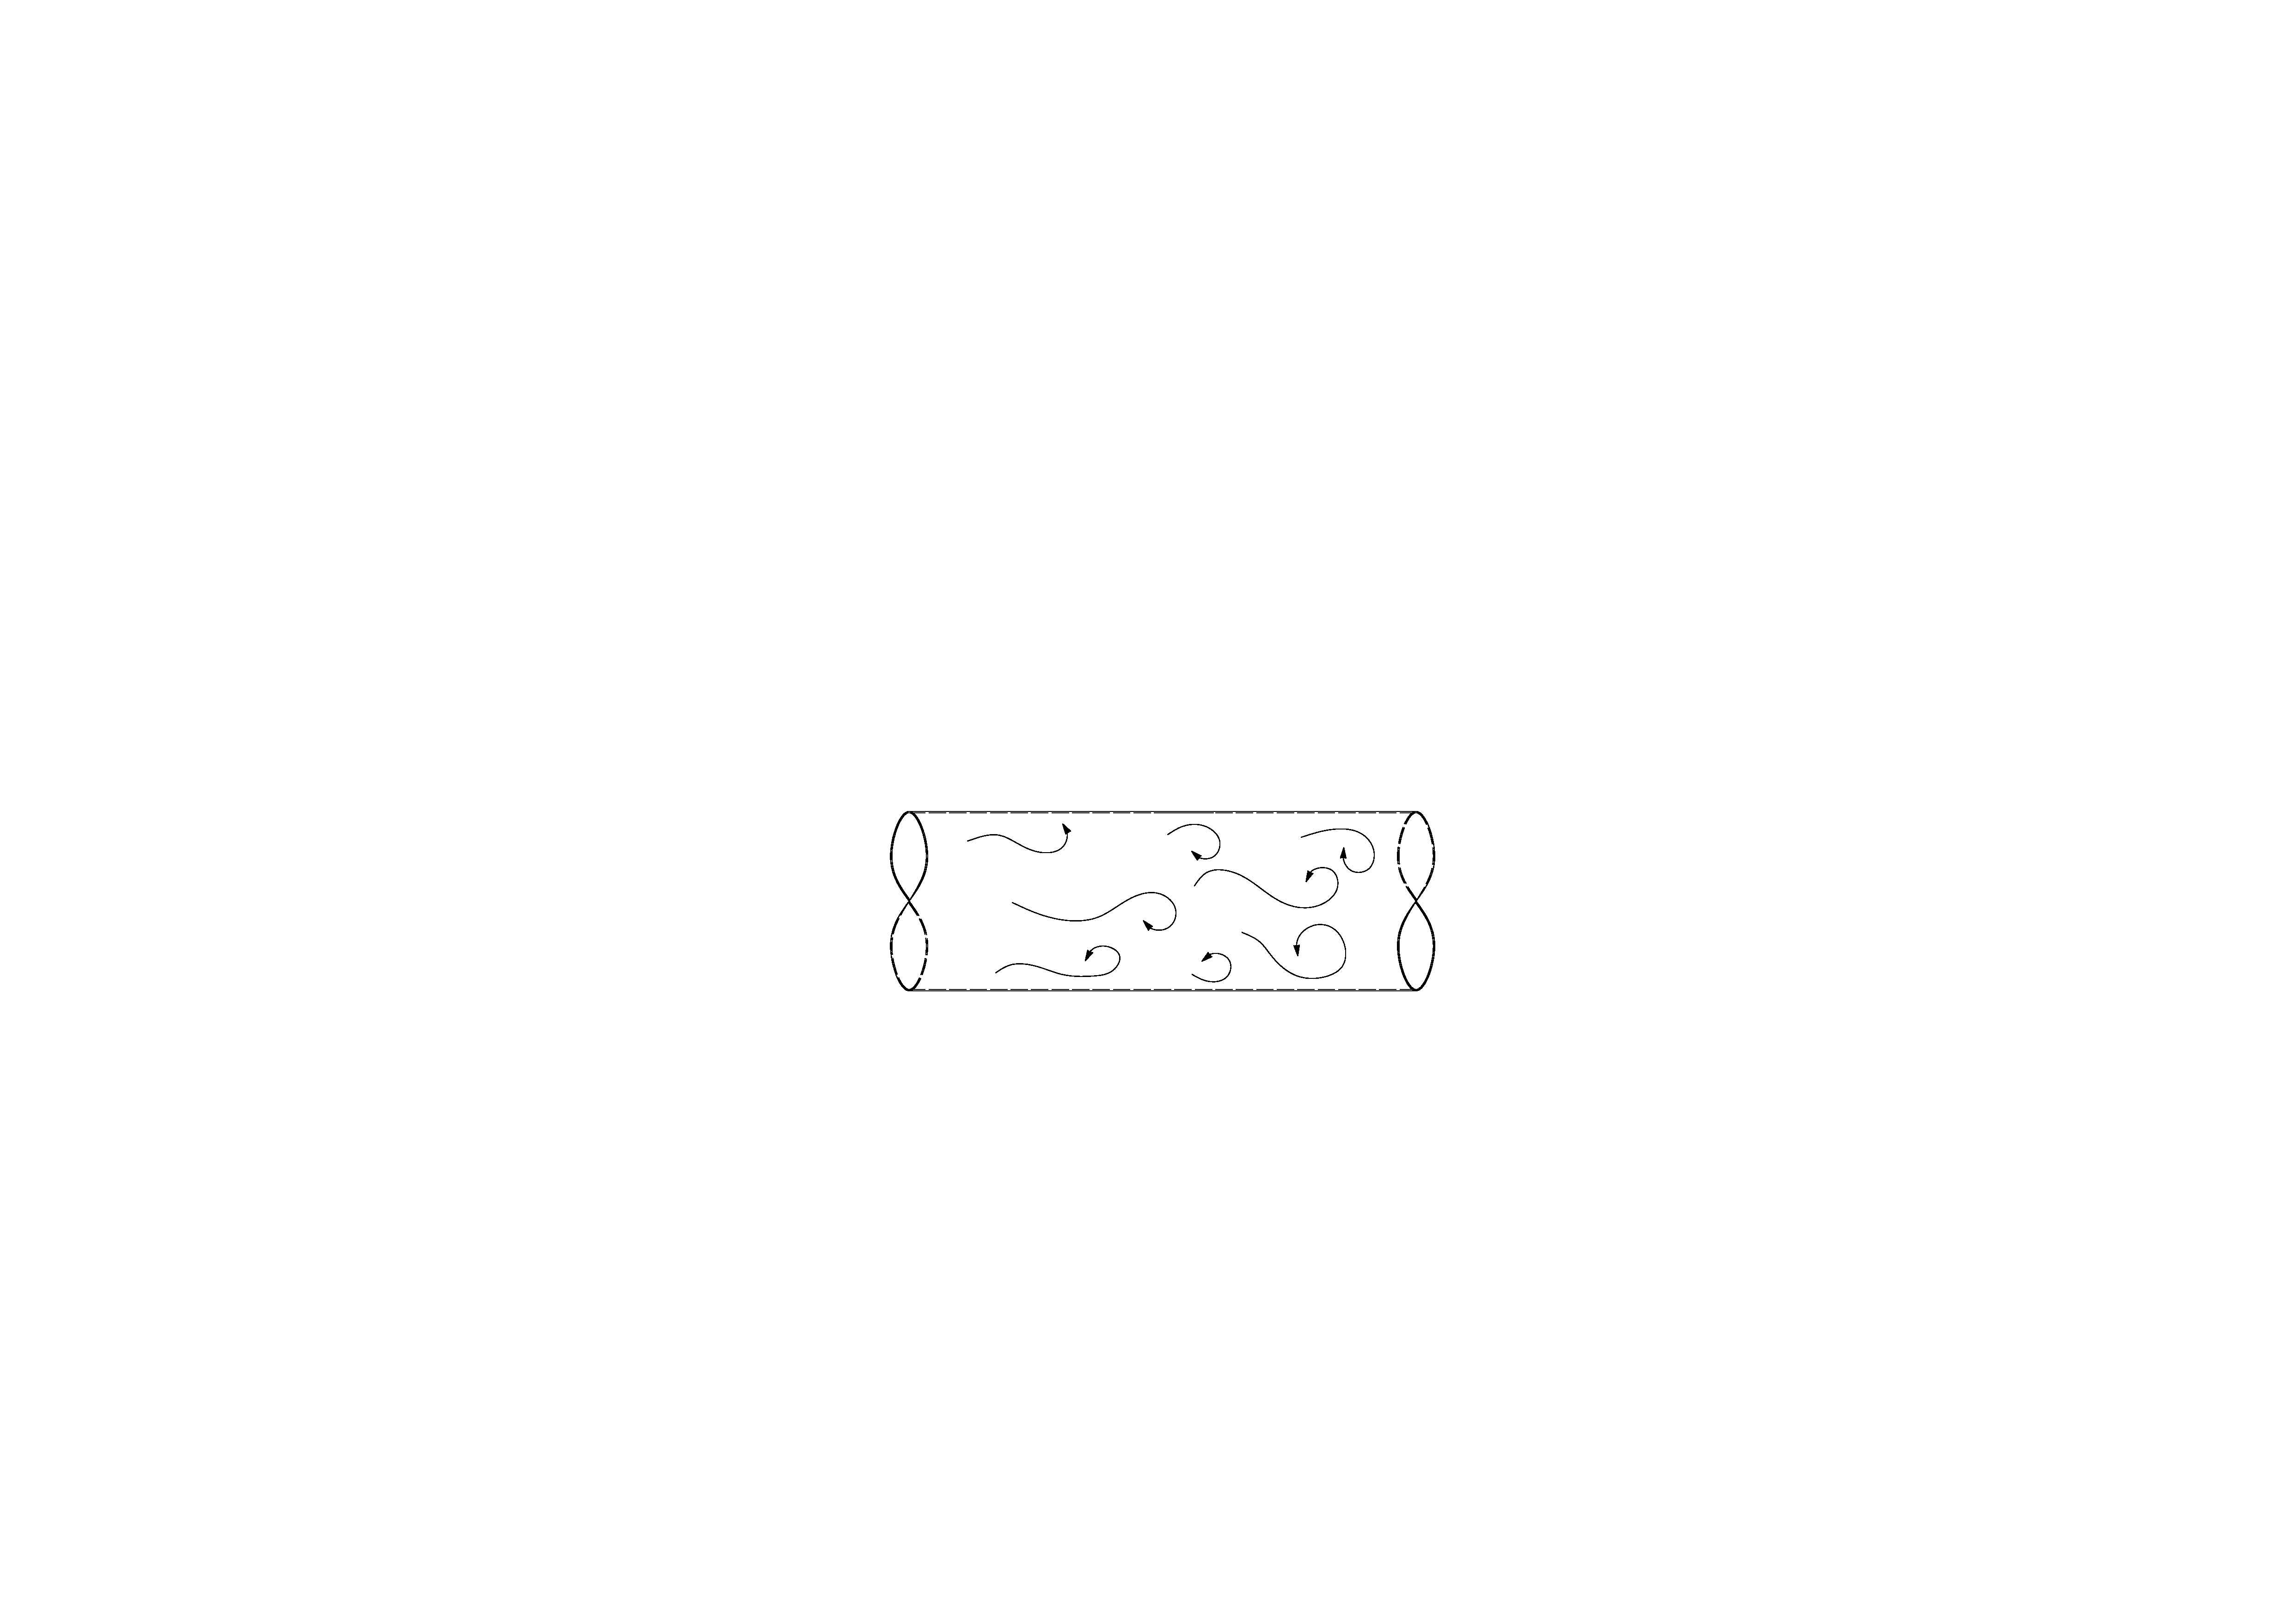
\includegraphics[width=.75\linewidth]{Figuras/EscTurbulento.pdf}
        \caption{Escoamento turbulento.}
        \label{fig:EscTurbulento}
      \end{subfigure}
    \\Fonte: Autoria Própria (\the\year).
\end{figure}

\end{document}
% %==================================================================================================
\chapter{Metodologia e cronograma} \label{MetodologiaCronograma}
%==================================================================================================

Tendo em vista a complexidade dos problemas em estudo, delimita-se os estudos dos problemas de interação fluido-estrutura considerando escoamento incompressível viscoso interagindo com estruturas reticuladas com grandes deslocamentos. Adota-se acoplamento particionado forte do tipo bloco-iterativo com método de malha móvel para o fluido empregando-se a descrição Lagrangiana-Euleriana Arbitrária (ALE). Essa abordagem é adotada por ser reconhecidamente robusta, modular e amplamente utilizada para análises de IFE.

Assim como os problemas a serem estudados, as implementações necessárias também são bastante complexas, sendo importante a adoção de uma metodologia de programação que aproveite os códigos disponíveis e ao mesmo tempo facilite alterações de tipos de elementos, modelos constitutivos, métodos de solução de sistemas e operações algébricas, e mais importante no contexto desta proposta, diferentes métodos de estabilização e diferentes modelos de turbulência.

Dessa forma, adota-se a linguagem de programação C++ orientada a objeto, em um sistema operacional Linux, uma vez que se é possível aproveitar diversos códigos já desenvolvidos pelo grupo de pesquisa, a saber, programa de elementos finitos para análise de escoamentos incompressíveis empregando-se elementos triangulares (2D) e tetraédricos (3D) com aproximações linear ou quadrática e programa para análise dinâmica não linear geométrica de estruturas de casca finas ou espessas empregando elementos triangulares cúbicos.

Para a solução da mecânica dos sólidos será empregado o MEF baseado em posições, aproveitando-se um programa para análise de cascas com cinemática de Reissner-Mindlin, já desenvolvido pelo grupo de pesquisa. A formulação baseada em posições emprega uma descrição Lagrangiana Total, sendo adotado o modelo constitutivo de Saint-Venant Kirchhoff  com a medida de deformação de Green-Lagrange. O elemento de casca utilizado possui 7 graus de liberdade por nó, a saber, 3 coordenadas de posição, 3 coordenadas de um vetor generalizado, inicialmente perpendicular à superfície média da casca, e 1 parâmetro de enriquecimento para permitir variação linear da deformação na direção da espessura. A aproximação das derivadas temporais do problema é feita com integrador temporal $alpha$-generalizado. O processo de solução dos sistema não linear é obtida por meio do método iterativo de Newton-Raphson. 

Já para a solução da mecânica dos fluidos fluido, parte-se de um código computacional para escoamentos bidimensionais e tridimensionais empregado a formulação estabilizada PSPG/SUPG do MEF e a descrição ALE, o que possibilita a representação de contornos móveis. Assim como no sólido, a aproximação temporal é dada pelo integrador $\alpha$-generalizado e o método de Newton-Raphson é empregado para a solução do sistema não linear. Neste código é parte desta proposta a implementação de elementos Taylor-Hood, com aproximação quadrática para velocidades e linear para pressão, a implementação da técnica de estabilização \LSIC (LSIC) para captura de vórtices, assim comoos modelos de turbulência RANS e LES e o modelo de estabilização VMS (implementações essas que já foram finalizadas).

Após o estudo e verificação isolada das ferramentas para solução do fluido e do sólido, parte-se para o acoplamento.
Para isso será adotado um modelo de acoplamento particionado forte do tipo bloco-iterativo, sendo a movimentação da malha do fluido realizada por meio de um problema fictício de elasticidade, considerando-se a malha do fluido como um sólido elástico com deslocamentos prescritos no contorno.

% \textcolor{red}{-Falar como você vai resolver o sólido (citar o programa de cascas disponível, a formulação empregada e a integração temporal adotada). Especificar se você vai implementar alguma coisa nele ou só utilizar.}

% \textcolor{red}{-Falar como você vai resolver o fluido considerando contornos móveis (citar o programa de fluido disponível, a formulação/elementos empregados e a integração temporal adotada). Especificar o que você vai implementar}

% \textcolor{red}{-Falar sobre a técnica de acoplamento a ser adotada para unir os códigos}

Será empregado o protocolo de processamento paralelo \textit{Message Passing Interface} (MPI), com utilização da biblioteca PETSc (\textit{Portable, Extensible Toolkit for Scientific Computation}) \cite{petsc-web-page}, a qual é reconhecidamente eficiente para solução de sistemas esparços que necessitem de alto desempenho computacional, tendo suporte para C++ e MPI.  As malhas serão geradas a partir do programa Gmsh \cite{geuzaine2009gmsh}, e os resultados serão interpretados graficamente por meio do visualizador Paraview \cite{ahrens2005paraview} e por meio do programa gnuPlot, no caso da geração de gráficos de linha 2D ou 3D. Nota-se que prioriza-se o uso de ferramentas computacionais livres e de código aberto para facilitar a distribuição e as atualizações da ferramenta computacional resultante.

%==================================================================================================
\section{Cronograma}
%==================================================================================================

% \textcolor{red}{As atividades estavam insuficientes para descrever o seu trabalho durante o curso (pode incluir as disciplinas, já que o cronograma é do trabalho de mestrado como todo). Adicionei outras atividades, verifique se não falta nada e atualize o cronograma (Pode incluir o exame de qualificação...).}

As atividades necessárias para se alcançar os objetivos desta pesquisa são organizadas da seguinte maneira:

\begin{enumerate}[label=\alph*.]
	\item\label{M:1} Cursar disciplinas do programa de mestrado;
	\item\label{M:2} Revisão bibliográfica a ser realizada de forma contínua ao longo de todo o trabalho, para que o mesmo se mantenha atualizado frente ao estado da arte durante toda sua execução;
	\item\label{M:3} Estudo das formulações estabilizadas do método dos elementos finitos para a solução de escoamentos incompressíveis com contornos móveis;
	\item\label{M:4} Estudo dos modelos de turbulência RANS e LES;
	\item\label{M:5} Estudo do código computacional para escoamentos incompressíveis disponível e implementações do modelo de estabilização VMS;
	\item\label{M:6} Implementação computacional dos modelos de turbulência no código de escoamentos incompressíveis;
	\item\label{M:7} Verificação dos modelos de turbulência implementados no contexto de escoamentos com contornos fixos a partir de exemplos presentes na literatura;
	\item\label{M:8} Estudo da formulação posicional do MEF para elementos de casca com cinemática de Reissner-Mindlin;
	\item\label{M:9} Exame de qualificação de mestrado;
	\item\label{M:10} Estudo e implementação do modelo de acoplamento particionado do tipo bloco-iterativo;
	\item\label{M:11} Verificação e Estudo dos modelos implementados no contexto dos problemas de iteração fluido-estrutura com elevados números de Reynolds;
	\item\label{M:12} Redação da dissertação e elaboração de artigos para revistas;
	\item \label{M:13} Defesa do mestrado.
\end{enumerate}

Essas atividades são organizadas cronologicamente, ao longo do tempo disponível para a conclusão do mestrado, de acordo com o cronograma da Tabela \ref{Cronograma}.

\definecolor{lightgray}{RGB}{153,153,153}
\definecolor{lightblue}{RGB}{126,194,216}

\begin{table}[h!]
	\caption{Cronograma de atividades}
	\fontsize{8}{14}\selectfont
	\centering
	\newcommand{\Rx}{\cellcolor{lightblue}}
	\newcommand{\Px}{\cellcolor{lightgray}}
	\begin{tabular}{|c|ccccccccc|cccccccccccc|cccc|}
		\hline
		\MR{2}{*}{Item} & \MC{9}{c|}{2022} & \MC{12}{c|}{2023} & \MC{4}{c|}{2024}                                                                                                                                     \\ \cline{2-26}
		                & A                & M                 & J                & J   & A   & S   & O   & N   & D   & J   & F   & M   & A   & M   & J   & J   & A   & S   & O   & N   & D   & J   & F   & M   & A   \\ \hline
		\ref{M:1}       & \Rx              & \Rx               & \Rx              & \Rx & \Rx & \Rx & \Rx & \Rx & \Rx &     &     &     &     &     &     &     &     &     &     &     &     &     &     &     &     \\ \hline
		\ref{M:2}       & \Rx              & \Rx               & \Rx              & \Rx & \Rx & \Rx & \Rx & \Rx & \Rx & \Rx & \Rx & \Rx & \Rx & \Rx & \Rx & \Rx & \Px & \Px & \Px & \Px & \Px & \Px & \Px & \Px &     \\ \hline
		\ref{M:3}       &                  &                   &                  &     & \Rx & \Rx & \Rx & \Rx & \Rx & \Rx & \Rx &     &     &     &     &     &     &     &     &     &     &     &     &     &     \\ \hline
		\ref{M:4}       &                  &                   &                  &     &     &     &     & \Rx & \Rx & \Rx & \Rx & \Rx & \Rx & \Rx &     &     &     &     &     &     &     &     &     &     &     \\ \hline
		\ref{M:5}       &                  &                   &                  &     &     &     &     &     &     &     & \Rx & \Rx & \Rx & \Rx &     &     &     &     &     &     &     &     &     &     &     \\ \hline
		\ref{M:6}       &                  &                   &                  &     &     &     &     &     &     &     &     &     &     & \Rx & \Rx & \Rx & \Px & \Px & \Px &     &     &     &     &     &     \\ \hline
		\ref{M:7}       &                  &                   &                  &     &     &     &     &     &     &     &     &     &     &     & \Rx & \Rx &     &     &     &     &     &     &     &     &     \\ \hline
		\ref{M:8}       &                  &                   &                  &     &     &     &     &     &     &     &     &     &     & \Rx & \Rx & \Rx &     &     &     &     &     &     &     &     &     \\ \hline
		\ref{M:9}       &                  &                   &                  &     &     &     &     &     &     &     &     &     &     &     &     &     & \Px &     &     &     &     &     &     &     &     \\ \hline
		\ref{M:10}      &                  &                   &                  &     &     &     &     &     &     &     &     &     &     &     &     &     & \Px & \Px & \Px & \Px &     &     &     &     &     \\ \hline
		\ref{M:11}      &                  &                   &                  &     &     &     &     &     &     &     &     &     &     &     &     &     &     &     &     & \Px & \Px & \Px & \Px &     &     \\ \hline
		\ref{M:12}      & \Rx              & \Rx               & \Rx              & \Rx & \Rx & \Rx & \Rx & \Rx & \Rx & \Rx & \Rx & \Rx & \Rx & \Rx & \Rx & \Rx & \Px & \Px & \Px & \Px & \Px & \Px & \Px & \Px &     \\ \hline
		\ref{M:13}      &                  &                   &                  &     &     &     &     &     &     &     &     &     &     &     &     &     &     &     &     &     &     &     &     &     & \Px \\ \hline
	\end{tabular}
	\label{Cronograma}
\end{table}

\begin{minipage}{\textwidth}
	\fontsize{8}{14}\selectfont
	\centering
	\colorbox{lightblue}{\rule{0pt}{10pt}\rule{10pt}{0pt}} Já realizado \quad
	\colorbox{lightgray}{\rule{0pt}{10pt}\rule{10pt}{0pt}} Pendente \quad
\end{minipage}

%==================================================================================================
\chapter{Formulação numérica para mecânica dos Fluidos} \label{EGDF}
%==================================================================================================

No presente capítulo serão apresentadas as equações que governam os escoamentos isotérmicos incompressíveis. Inicialmente apresenta-se a formulação em descrição Euleriana, onde se considera um domínio fixo na configuração atual do escoamento (Seção \ref{CFD-E}). Em seguida essa formulação é expandida para a descrição Lagrangiana-Euleriana Arbitrária (ALE), a qual permite a movimentação da malha, independentemente da movimentação das partículas do fluido (Seção \ref{CFD-ALE}). Posteriormente, por meio do método dos resíduos ponderados, obtém-se a forma fraca para a solução do problema com uso da técnica dos elementos finitos (Seção \ref{FSD}), sendo as técnicas de estabilização adotadas apresentas na seção \ref{STAB}.

%==================================================================================================
\section{Descrição Euleriana} \label{CFD-E}
%==================================================================================================

\subsection{Conservação da massa}
Em descrição Euleriana, é possível se obter uma expressão que defina a conservação de massa (também denominada como Equação da Continuidade) do fluido, considerando um elemento infinitesimal permeável, que definirá o volume de controle, conforme ilustrado na Figura \ref{fig:BalMas}, em que $\BB{u}$ é o valor da velocidade na posição atual $\BB{y}$ e $\rho$ é a massa específica do fluido nesse ponto.

\begin{figure}[h!]
    \centering
    \caption{Taxa de fluxo de massa em um elemento infinitesimal permeável.}
    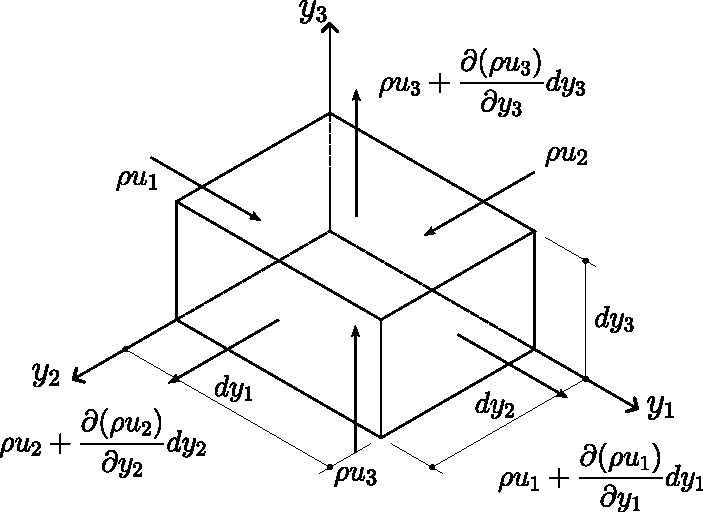
\includegraphics[width=.5\linewidth]{Figuras/BalMas.pdf}
    \\Fonte: Autoria Própria (\the\year).
    \label{fig:BalMas}
\end{figure}

A variação da massa contida neste elemento é dada por:

\begin{equation}
    dm=dm_0+\apdery{dm}{t}dt\text{,}
\end{equation}

\noindent a partir de onde expressa-se o balanço de massa no elemento por:

\begin{equation}
    \frac{D\rho}{Dt}+\rho \Ny\cdot\BB{u}=\dTime{\rho}+\Ny\cdot(\rho \BB{u})=0\text{,}
    \label{eq:BalMas}
\end{equation}

\noindent sendo $D\rho/Dt$ a derivada material, definida para um escalar $\phi$ qualquer como:

\begin{equation}
    \frac{D\phi}{Dt}=\dTime{\phi}+(\BB{u}\cdot\Ny)\phi\text{,}
\end{equation}

\noindent em que o ponto sobre a variável representa a derivada temporal da mesma, $\Ny\cdot(\cdot)$ é o operador divergente e $\Ny(\cdot)$ é o operador gradiente, que para uma função escalar $g$ é definido por \eqref{eq:grad1} e para uma função vetorial é definido por \eqref{eq:grad2}:

\begin{subequations}
    \begin{align}
         & \Ny g=\der{g}{\BB{y}}\equiv\der{g}{y_i}            &  & \text{, com }i=1,2,\hdots,n_{sd}\text{ e} \label{eq:grad1}    \\
         & \Ny\BB{g}=\der{\BB{g}}{\BB{y}}\equiv\der{g_i}{y_j} &  & \text{, com }i\text{ e }j=1,2,\hdots,n_{sd}, \label{eq:grad2}
    \end{align}
\end{subequations}

\noindent sendo $n_{sd}=2$ ou $3$ a dimensão do problema em análise.

Para escoamentos incompressíveis, Eq. \eqref{eq:BalMas} fica reduzida a:

\begin{equation}
    \Ny\cdot\BB{u}=0\text{,}\label{eq:incomp}
\end{equation}

\noindent denominada equação da continuidade ou condição de incompressibilidade.

\subsection{Conservação da quantidade de movimento}
O fluxo da Quantidade de Movimento linear (ou de \textit{Momentum} Linear) no elemento infinitesimal permeável é ilustrado na Figura \ref{fig:ConQtdMov}.

\begin{figure}[h!]
    \centering
    \caption{Fluxo de quantidade de movimento em um elemento infinitesimal permeável.}
    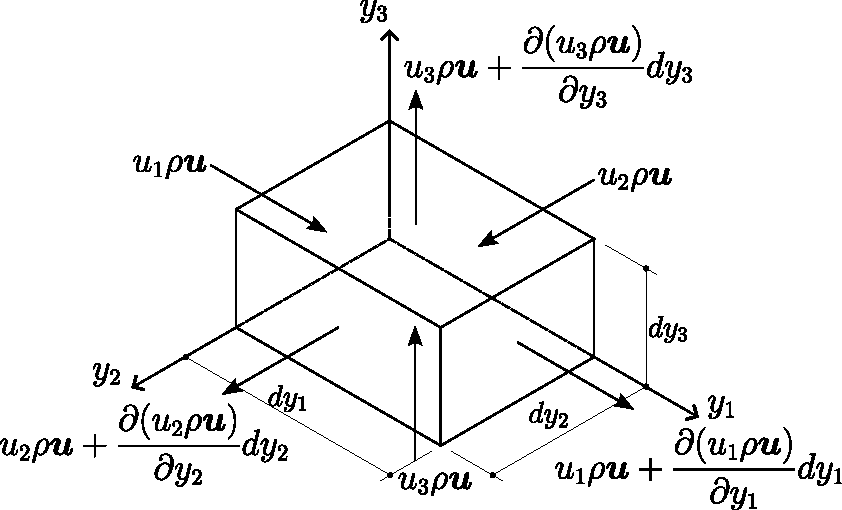
\includegraphics[width=.55\linewidth]{Figuras/ConQtdMov.pdf}
    \\Fonte: Autoria Própria (\the\year).
    \label{fig:ConQtdMov}
\end{figure}

Realizando-se o balanço da quantidade de movimento sobre este elemento, e aplicando-se o princípio da conservação da quantidade de movimento, pode-se escrever:

\begin{equation}
    \apdery{(\rho \BB{u})}{t}+\Ny\cdot(\rho \BB{u}\otimes\BB{u})-\BB{q}=\BB{0}\text{,}
    \label{eq:ConQtdMov}
\end{equation}

\noindent onde $\BB{q}$ representa a força resultante por unidade de volume que atua no elemento, ou seja, $\BB{q}=d\Fres/dV$. Entretanto, não é de interesse escrever a equação \eqref{eq:ConQtdMov} em termos desse vetor $\BB{q}$, mas em termos do tensor de tensões de Cauchy ($\tens$) e das forças de volume. Para isso, considera-se o diagrama de corpo livre do elemento infinitesimal ilustrado na Figura \ref{fig:EqFor}, onde são representadas apenas as componentes de tensão e de forças de volume atuantes na direção $y_1$.

\begin{figure}[h!]
    \centering
    \caption{Componentes de forças atuantes no elemento infinitesimal na direção $y_1$.}
    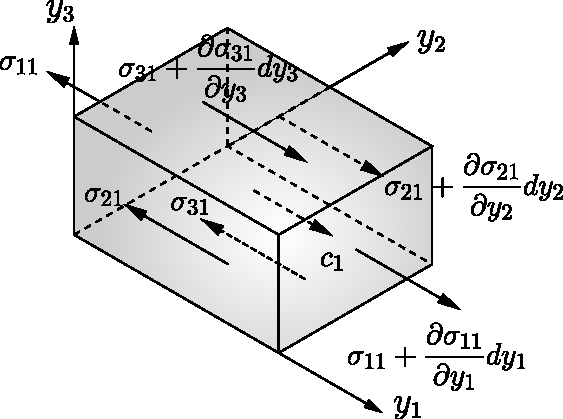
\includegraphics[width=.5\linewidth]{Figuras/EqFor.pdf}
    \\Fonte:Autoria Própria (\the\year).
    \label{fig:EqFor}
\end{figure}

Fazendo o equilíbrio de forças na direção de $y_1$, obtém-se que:

\begin{equation}
    q_1=\der{\sigma_{11}}{y_1}+\der{\sigma_{21}}{y_2}+\der{\sigma_{31}}{y_3}+c_1\text{,}
\end{equation}

\noindent procedendo-se analogamente para as demais direções, e sabendo-se da simetria de $\tens$, tem-se que:

\begin{equation}
    \BB{q}=\Ny\cdot\tens+\BB{c}\text{.}
    \label{eq:RelQSig}
\end{equation}

Substituindo \eqref{eq:RelQSig} em \eqref{eq:ConQtdMov} e aplicando a condição de incompressibilidade, obtém-se a equação da conservação da quantidade de movimento escrita em termos de tensões:

\begin{equation}
    \rho\bigpar{\dTime{\BB{u}}+(\BB{u}\cdot\Ny)\BB{u}-\BB{f}}-\Ny\cdot\tens=\BB{0}\text{,}
    \label{eq:ConQtdMov-2}
\end{equation}

\noindent em que $\BB{c}=\rho\BB{f}$, tal que $\BB{f}$ é uma força por unidade de massa. Além disso, também é possível escrever a equação \eqref{eq:ConQtdMov-2} utilizando a notação de derivada material como:

\begin{equation}
    \rho\bigpar{\frac{D\BB{u}}{Dt}-\BB{f}}-\Ny\cdot\tens=\BB{0}\text{.}
    \label{eq:ConQtdMov-3}
\end{equation}

Já o domínio em que essas equações são válidas pode ser definido como $\Omega\subset\mathbb{R}^{n_{sd}}$, tal que $\Omega$ possui uma fronteira $\Gamma=\partial\Omega$, tal que a parte dessa fronteira onde se impõem condições de contorno essenciais é denominada como fronteira de Dirichlet ($\Gamma_D$) e a parte onde há prescrição de forças de superfície é denotada como fronteira de Neumann ($\Gamma_N$), conforme pode ser visualizado na Figura \ref{fig:Dom}.

\begin{figure}[h!]
    \centering
    \caption{Domínio e condições de contorno para os problemas de mecânica dos fluidos.}
    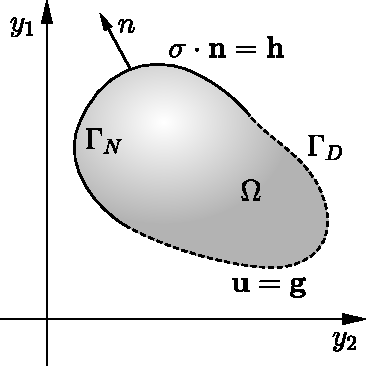
\includegraphics[width=.35\linewidth]{Figuras/Dom}
    \\Fonte: Autoria Própria (\the\year).
    \label{fig:Dom}
\end{figure}

Dessa forma, o problema a ser resolvido segue as equações:

\begin{equation}
    \left\{
    \begin{array}{ll}
        \rho\bigpar{\dTime{\BB{u}}+(\BB{u}\cdot\Ny)\BB{u}-\BB{f}}-\Ny\cdot\tens=\BB{0} & \text{ em }\Omega\text{,}   \\
        \Ny\cdot\BB{u}=0                                                               & \text{ em }\Omega\text{,}   \\
        \tens\cdot\BB{n}=\BB{h}                                                        & \text{ em }\Gamma_N\text{,} \\
        \BB{u}=\BB{g}                                                                  & \text{ em }\Gamma_D\text{,}
    \end{array}
    \right.
    \label{eq:NS-Euler}
\end{equation}

\noindent que governam o os escoamentos incompressíveis de Navier-Stokes em descrição Euleriana \cite{bazilevs2013computational,bazilevs2010large,bazilevs2007variational,hughes2002variational,hughes2000large}.

%==================================================================================================
\section{Descrição Lagrangiana-Euleriana Arbitrária} \label{CFD-ALE}
%==================================================================================================

A descrição Lagrangiana-Euleriana Arbitrária (\textit{Arbitrary Lagrangian-Eulerian} - ALE) originou-se do trabalho de \citeonline{donea1982arbitrary}. São considerados 3 domínios, $\Omega_0$, $\Omega$ e $\hat{\Omega}$, que representam, respectivamente, os domínios do contínuo em sua configuração inicial e atual e o domínio da malha, que desenvolve movimento independente do movimento do contínuo, como ilustrado na Figura \ref{Fig:ALE}.

\begin{figure}[h!]
    \centering
    \caption{Descrição Lagrangiana-Euleriana Arbitrária.}
    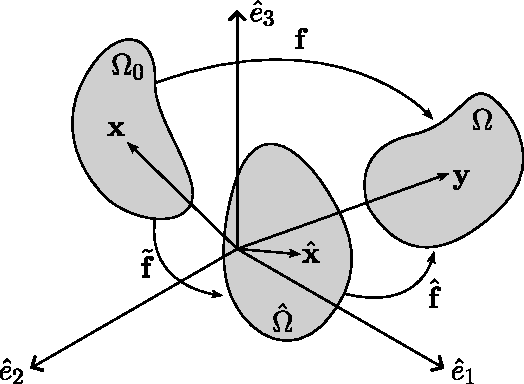
\includegraphics[width=.45\linewidth]{Figuras/ALE.pdf}
    \label{Fig:ALE}
    \\Fonte: Autoria Própria (\the\year).
\end{figure}

As coordenadas $\BB{x}$, $\BB{y}$ e $\HBB{x}$ representam as coordenadas de um ponto nos domínios $\Omega_0$, $\Omega$ e $\hat{\Omega}$, respectivamente. Já as funções $\fmc(\BB{x},t)=\BB{y}(\BB{x},t)$, $\tfmc(\BB{x},t)=\HBB{x}(\BB{x},t)$ e $\hfmc(\HBB{x},t)=\BB{y}(\HBB{x},t)$ são funções que mapeiam o domínio inicial do fluido para o atual, o domínio inicial  do fluido para o domínio inicial da malha, e o domínio da malha para a configuração atual do fluido, que é coincidente com a configuração atual da malha.

Com isso, podem-se escrever os gradientes dessas funções:

\begin{subequations}
    \begin{equation}
        \FMC=\der{(\fmc(\BB{x},t),t)}{(\BB{x},t)}=\begin{bmatrix}
            \Nx\BB{y} & \BB{u} \\\BB{0}\trans&1
        \end{bmatrix}\text{,}\label{F2}
    \end{equation}
    \begin{equation}
        \TFMC=\der{(\tfmc(\BB{x},t),t)}{(\BB{x},t)}=\begin{bmatrix}
            \Nx\HBB{x} & \tilde{\BB{u}} \\\BB{0}\trans&1
        \end{bmatrix}\text{, e}\label{F1}
    \end{equation}
    \begin{equation}
        \HFMC=\der{(\hfmc(\HBB{x},t),t)}{(\HBB{x},t)}=\begin{bmatrix}
            \Nxh\BB{y} & \uhat \\\BB{0}\trans&1
        \end{bmatrix}\text{,}\label{F3}
    \end{equation}
    \label{eq:GradFun}
\end{subequations}

\noindent nos quais $\BB{u}=\partial\BB{y}/\partial t|_{\BB{x}}$, $\tilde{\BB{u}}=\partial\HBB{x}/\partial t|_{\BB{x}}$ e $\uhat=\partial\BB{y}/\partial t|_{\HBB{x}}$. Além disso, vale ressaltar que $\fmc(\BB{x},t)=\hfmc(\tfmc(\BB{x},t),t)$, portanto $\FMC=\HFMC\cdot\TFMC$, ou seja:

\begin{equation}
    \begin{bmatrix}\Nx\BB{y}&\BB{u}\\\BB{0}\trans&1\end{bmatrix}=
    \begin{bmatrix}\Nxh\BB{y}&\uhat\\\BB{0}\trans&1\end{bmatrix}\cdot
    \begin{bmatrix}\Nx\HBB{x}&\tilde{\BB{u}}\\\BB{0}\trans&1\end{bmatrix}\text{,}
    \label{F4}
\end{equation}

\noindent que possui, como uma de suas consequências:

\begin{equation}
    \BB{u}=\Nxh\BB{y}\cdot\tilde{\BB{u}}+\uhat\text{, ou}
    \label{u1}
\end{equation}

\begin{equation}
    \tilde{\BB{u}}=\Ny\HBB{x}\cdot(\BB{u}-\uhat)\text{.}
    \label{w1}
\end{equation}

Assim é possível definir a derivada material na descrição ALE. Para isso seja uma propriedade $\phi(\BB{y},t)$ escrita em termos da configuração atual, igual a $\phi^*(\HBB{x},t)$ quando escrita em termos da configuração de referência e igual a $\phi^{**}(\BB{x},t)=\phi^*(\tfmc(\BB{x},t),t)$ quando escrita em termos da configuração inicial. Logo:


\begin{equation}
    \der{\phi^{**}(\BB{x},t)}{(\BB{x},t)}=\der{\phi^*(\HBB{x},t)}{(\HBB{x},t)}\cdot\der{\tfmc(\BB{x},t)}{(\BB{x},t)}\text{, ou}
    \label{phi1}
\end{equation}

\begin{equation}
    \begin{bmatrix}\Nx\phi^{**}&\dTimex{\phi^{**}}\end{bmatrix}=
    \begin{bmatrix}\Nxh\phi^{*}&\dTimexh{\phi^{*}}\end{bmatrix}\cdot
    \begin{bmatrix}\Nx\HBB{x}&\tilde{\BB{u}}\\\BB{0}\trans&1\end{bmatrix}
    \text{.}
    \label{phi2}
\end{equation}

\noindent Portanto:

\begin{equation}
    \dTimex{\phi^{**}}=\Nxh\phi^{*}\cdot\tilde{\BB{u}}+\dTimexh{\phi^{*}}\text{.}
    \label{phi3}
\end{equation}

Substituindo \ref{w1} em \ref{phi3}, obtém-se que:

\[\dTimex{\phi^{**}}=\Nxh\phi^{*}\cdot\Ny\HBB{x}\cdot(\BB{u}-\uhat)+\dTimexh{\phi^{*}}\]

\[\dTimex{\phi^{**}}=\dTimexh{\phi^{*}}+(\BB{u}-\uhat)\cdot\Ny\phi^{*}\]

Dessa maneira, remove-se os sobrescritos * e ** e define-se a derivada material na descrição ALE como:

\begin{equation}
    \frac{D\phi}{Dt}=\dTime{\phi}+(\BB{u}-\uhat)\cdot\Ny\phi\text{.}
    \label{eq:DerMat2}
\end{equation}

%==================================================================================================
\subsection{Equações governantes na descrição ALE}
%==================================================================================================

Substituindo-se $\phi$ por $\rho$ e aplicando-se a Eq. \eqref{eq:DerMat2} na Eq. \eqref{eq:BalMas}, a conservação da massa na descrição ALE é dada por:

\begin{equation}
    \dTime{\rho}+(\BB{u}-\uhat)\cdot\Ny\rho+\rho\Ny\cdot\BB{u}=0\text{,}
\end{equation}

\noindent que para escoamentos incompressíveis, onde $\frac{D \rho}{t}=0$, implica em:

\begin{equation}
    \Ny\cdot\BB{u}=0\text{,}
    \label{eq:ALE-cont}
\end{equation}

Já a Equação da Conservação da Quantidade de Movimento na descrição ALE pode ser obtida fazendo $\mathbf{\phi}=\BB{u}$ na Eq. \eqref{eq:DerMat2} e substituindo em Eq. \eqref{eq:ConQtdMov-3}, resultando:

\begin{equation}
    \rho\bigpar{\dTime{\BB{u}}+((\BB{u}-\uhat)\cdot\Ny)\BB{u}-\BB{f}}-\Ny\cdot\tens=\BB{0}\text{.}
    \label{eq:ALE-mov}
\end{equation}

Assim, os escoamentos de Navier-Stokes incompressíveis em descrição ALE são governados pelas equações \cite{bazilevs2013computational}:

\begin{equation}
    \left\{
    \begin{array}{ll}
        \rho\bigpar{\dTime{\BB{u}}+((\BB{u}-\HBB{u})\cdot\Ny)\BB{u}-\BB{f}}-\Ny\cdot\tens=\BB{0} & \text{ em }\Omega\text{,}    \\
        \Ny\cdot\BB{u}=0                                                                         & \text{ em }\Omega\text{,}    \\
        \tens\cdot\BB{n}=\BB{h}                                                                  & \text{ em }\Gamma_N\text{ e} \\
        \BB{u}=\BB{g}                                                                            & \text{ em }\Gamma_D\text{.}
    \end{array}
    \right.
    \label{eq:NS-ALE}
\end{equation}

%==================================================================================================
\section{Modelo Constitutivo} \label{MC}
%==================================================================================================

O modelo constitutivo adotado para o fluido é o de escoamentos Newtonianos incompressíveis, o qual relaciona o tensor de tensões de Cauchy com a taxa de deformação e a pressão de acordo com:

\begin{equation}
    \tens=\BB{\tau}-p\BB{I}\text{,}\label{eq:const1}
\end{equation}

\noindent onde $\BB{I}$ é o tensor identidade de segunda ordem e $\BB{\tau}$ é o tensor de tensões viscosas (ou tensor desviador), que para fluidos Newtonianos é dado por:

\begin{equation}
    \BB{\tau}=\BB{\mathfrak{D}}:\dDef\text{,}
\end{equation}

\noindent em que $\BB{\mathfrak{D}}$ é o tensor constitutivo de quarta ordem:

\begin{equation}
    \BB{\mathfrak{D}}=2\mu\BB{\mathbb{I}}+\lambda\BB{I}\otimes\BB{I}\text{,}
\end{equation}

\noindent sendo $\BB{\mathbb{I}}$ o tensor identidade de quarta ordem, $\mu$ a viscosidade dinâmica do fluido e $\dDef$ o tensor de taxa de deformação, definido como:

\begin{equation}
    \dDef=\frac{1}{2}\bigpar{\Ny\BB{u}+\NyT\BB{u}}\text{.}\label{eq:deftax1}
\end{equation}

Assim, o tensor desviador pode ser escrito da seguinte maneira:

\[
    \BB{\tau}=(2\mu\BB{\mathbb{I}}+\lambda\BB{I}\otimes\BB{I}):\dDef=2\mu\BB{\mathbb{I}}:\dDef+\lambda\BB{I}\otimes\BB{I}:\dDef
\]

\noindent resultando em:

\begin{equation}
    \BB{\tau}=2\mu\dDef+\lambda\tr{(\dDef)}\BB{I}\text{,}
\end{equation}

\noindent sendo $\tr{(\dDef)}$ o traço do tensor $\dDef$.

Já para o caso de escoamentos incompressíveis, verifica-se que $\tr{(\dDef)}=0$, fazendo com que \eqref{eq:const1} possa ser escrita como:

\begin{equation}
    \tens=\mu(\Ny\BB{u}+\NyT\BB{u})-p\BB{I}\text{.}\label{eq:ModConst}
\end{equation}

%INTERPRETAÇÃO DA EQUAÇÃO DO MOVIMENTO
Logo é possível substituir o modelo constitutivo na equação da conservação da quantidade de movimento apresentada em \eqref{eq:NS-ALE} e realizar algumas manipulações algébricas para se obter:

\begin{equation}
    \dTime{\BB{u}}+((\BB{u}-\HBB{u})\cdot\Ny)\BB{u}=\BB{f}-\frac{\Ny p}{\rho}+\nu\Lapl\BB{u}\text{.}
    \label{eq:NS-ALE-2}
\end{equation}

\noindent em que $\Lapl(\cdot)=\Ny\cdot\Ny(\cdot)$ é o operador laplaciano e $\nu=\mu/\rho$ a viscosidade cinemática.

Essa equação representa a primeira lei de Euler (generalização da a segunda lei de Newton para um meio contínuo), sendo o lado esquerdo referente às acelerações, onde $\left.\partial\BB{u}/\partial t\right|_{\BB{y}}$ representa a taxa de variação local de velocidade em um elemento ao longo do tempo e $((\BB{u}-\HBB{u})\cdot\Ny)\BB{u}$ representa a aceleração convectiva, referente à variação de velocidade no espaço. Já o lado direito representa as forças por unidade de massa, sendo $\BB{f}$ devida às forças de corpo, $\Ny p/\rho$ devida à pressão interna do fluido e $\nu\Lapl\BB{u}$ devido às forças viscosas (ou forças de difusão).

% Os escoamentos isotérmicos incompressíveis são governados pelos princípios da conservação da massa e da conservação da quantidade de movimento, que na descrição ALE resultam respectivamente em (ver anexo \ref{Ap:CFD} para maiores detalhes):
% 
% \begin{subequations}
%     \begin{align}
%          & u_{i,i}=0                                                         &  & \text{ em }\Omega\text{,}   \label{eq:CFD-NS2} \\
%          & \rho\bigpar{\dot{u}_i+(u_j-\hat{u}_j)u_{i,j}-f_i}-\sigma_{ji,j}=0 &  & \text{ em }\Omega\text{,}   \label{eq:CFD-NS1} %\\
%         % & \sigma_{ij}n_i=h_j                                                &  & \text{ em }\Gamma_N\text{,} \label{eq:CFD-NS3} \\
%         % & u_j=g_j                                                           &  & \text{ em }\Gamma_D\text{,} \label{eq:CFD-NS4}
%     \end{align}
%     \label{eq:CFD-NS}
% \end{subequations}
% 
% Neste capítulo apresenta-se a formulação numérica para solução do problema de dinâmica dos fluidos no contexto da formulação estabilizada \ref{VMS} em descrição ALE. Por fim, são desenvolvidas as formulações dos modelos de turbulência RANS \ref{RANS} e LES \ref{LES}. Análises numéricas já realizadas empregando-se essas formulações são apresentas nos Apêndices \ref{Ap:Cavity} ao \ref{Ap:cylinder}.

%==================================================================================================
\section{Formulação Semi-Discreta} \label{FSD}
%==================================================================================================

Para a obtenção da forma fraca das equações \eqref{eq:NS-ALE}, parte-se do método dos resíduos ponderados. Assim, sejam os espaços de dimensões infinitas $\script{S}_u$ e $\script{S}_p$ das funções tentativas para os campos de velocidades e pressões, respectivamente, tal que \cite{bazilevs2013computational,fernandes2020tecnica}:

\begin{equation}
    \script{S}_u=\left\{\BB{u}|\BB{u}(\cdot,t)\in H^1(\Omega),\BB{u}=\BB{g}\text{ em }\Gamma_D\right\}\text{ e}
\end{equation}

\begin{equation}
    \script{S}_p=\left\{p|p(\cdot)\in L^2(\Omega),\int_\Omega{pd\Omega}=0\text{ se }\Gamma=\Gamma_D\right\}\text{,}
\end{equation}

\noindent em que $H^1(\Omega)$ representa o espaço de funções polinomiais com derivadas de quadrado integrável em $\Omega$ e $L^2(\Omega)$ representa o espaço de funções polinomiais de quadrado integrável em $\Omega$, ou seja:

\begin{equation}
    H^1(\Omega)=\left\{u\in L^2(\Omega);\der{u}{\BB{x}}\in L^2(\Omega)\right\}\text{ e}
\end{equation}

\begin{equation}
    L^2(\Omega)=\left\{u\big|\int_\Omega{|u|^2d\Omega}<\infty\right\}\text{.}
\end{equation}

Sejam ainda os espaços das funções testes para a conservação de massa e conservação da quantidade de movimento $\script{V}_p$ e $\script{V}_u$, respectivamente, tais que:

\begin{equation}
    \script{V}_p=\script{S}_p\text{ e}
\end{equation}

\begin{equation}
    \script{V}_u=\left\{\BB{w}|\BB{w}(\cdot)\in(H^1(\Omega))^{n_{sd}},\BB{w}=\BB{0}\text{ em }\Gamma_D\right\}\text{.}
\end{equation}

Dessa forma, ponderando-se as equações \eqref{eq:ALE-mov} e \eqref{eq:ALE-cont} respectivamente por $\BB{w}$ e $q$, tal que $q\in\script{V}_p$ e integrando-se sobre o domínio $\Omega$, obtém-se:

\begin{equation}
    \intDom{\BB{w}\cdot\bigpar{\rho\bigpar{\dTime{\BB{u}}+((\BB{u}-\HBB{u})\cdot\Ny)\BB{u}-\BB{f}}-\Ny\cdot\tens}}+\intDom{q\Ny\cdot\BB{u}}=0\text{.}
\end{equation}

Separando-se a parcela que contém o tensor de tensões de Cauchy da primeira integral, tem-se que:

\[\intDom{\BB{w}\cdot\rho\bigpar{\dTime{\BB{u}}+((\BB{u}-\HBB{u})\cdot\Ny)\BB{u}-\BB{f}}}-\intDom{\BB{w}\cdot(\Ny\cdot\tens)}+\intDom{q\Ny\cdot\BB{u}}=0\text{.}\]

Fazendo a integração por partes da parcela que foi separada e considerando o Teorema da Divergência, chega-se a:

\begin{equation}
    \begin{split}
        &\intDom{\BB{w}\cdot\rho\bigpar{\dTime{\BB{u}}+((\BB{u}-\HBB{u})\cdot\Ny)\BB{u}-\BB{f}}}-\intNeumann{\BB{w}\cdot\BB{h}}+\\
        &\intDom{\Ny\BB{w}:\tens}+\intDom{q\Ny\cdot\BB{u}}=0\text{.}
    \end{split}
    \label{eq:WeakForm2}
\end{equation}
Assim, o problema, fica definido como: dados $\BB{f}$, $\BB{g}$, $\BB{h}$ e $\HBB{u}$, em que $\BB{h}=\tens\cdot\BB{n}$ é o valor prescrito de força de superfície em $\Gamma_N$, determinar $(\BB{u},p)\in\script{S}_u\times\script{S}_p$ tal que $\forall\BB{w}\in\script{V}_u$ e $\forall q\in\script{V}_p$ em um intervalo $t\in(0,T)$, a equação \eqref{eq:WeakForm2} seja satisfeita.

A solução desse problema, entretanto, pode levar à resultados com variações espúrias em problemas de convecção dominante caso seja considerado o método clássico de Galerkin (Bubnov-Galerkin), como mencionado em \cite{fernandes2020tecnica,donea2003finite,brooks1982streamline}. Uma solução eficiente e consistente para isso é o emprego da técnica SUPG, como mencionado anteriormente. Além disso, vale observar que a adoção do grau de aproximação dos campos de velocidades e de pressões não pode ser feita de maneira descuidada, uma vez que, para conduzir a uma sistema com unicidade de solução, os espaços de funções para velocidade e pressão devem observar as condições \textit{Ladyzhenskaya-Babuška-Brezzi} (LBB), que, como uma condição necessária, porém não suficiente, aponta a necessidade de se adotar funções para pressão de ordem inferior às adotadas para velocidade, tal que \cite{donea2003finite}:

\begin{equation}
    \dim{\script{V}_p^h}\leq\dim{\script{V}_u^h}\text{.}
\end{equation}

A escolha dos espaços de aproximação da velocidade e da pressão depende da seguinte condição suficiente:

\begin{equation}
    \inf_{q^h\in\script{V}_p^h}{\sup_{\BB{w}^h\in\script{V}_u^h}{\frac{(q^h,\BB{\nabla}\cdot\BB{w}^h)}{\norm{q}_0\norm{\BB{w}^h}_1}}}\geq\beta>0\text{,}
\end{equation}

\noindent em que $\beta$ é uma constante independente do tamanho da malha.

Como pode-se observar, a determinação de combinações de espaços de aproximações que atendam às condições LBB não é trivial, sendo que elementos estáveis são identificados em diferentes trabalhos. \citeonline{donea2003finite} apresentam alguns elementos finitos que atendem às condições LBB (denominados de Elementos Taylor-Hood), sendo alguns ilustrados na Figura \ref{fig:Taylor-Hood}.

\begin{figure}[h!]
    \centering
    \caption{Elementos Taylor-Hood.}
    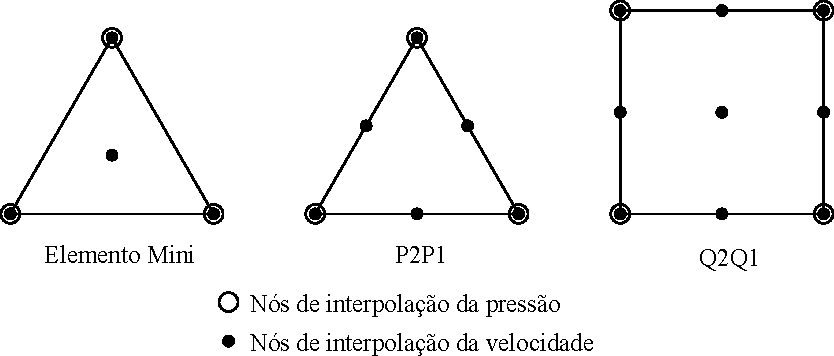
\includegraphics[width=.65\linewidth]{Figuras/Taylor-Hood.pdf}
    \\Fonte: \citeonline{fernandes2020tecnica} - Adaptado.
    \label{fig:Taylor-Hood}
\end{figure}

Uma alternativa ao uso de Elementos Taylor-Hood, e que torna os métodos mais flexíveis, é o emprego de formulações estabilizadas, como a técnica PSPG \cite{tezduyar1991stabilized}.

Outra formulação que é eficiente tanto para a estabilização da convecção quanto do campo de pressão, e que engloba os mesmos termos da estabilização SUPG/PSPG e ainda introduzindo outros termos estabilizantes de forma consistente, é a formulação VMS \cite{bazilevs2013computational}.

%==================================================================================================
\section{Técnicas de estabilização}\label{STAB}
%==================================================================================================

A utilização do MEF para descrever o comportamento de escoamentos incompressíveis possui duas fontes principais de instabilidades, que são associadas à convecção e à pressão \cite{tezduyar1991stabilized}. Nesse sentido se desenvolveram técnicas de estabilização que visam a minimizar ou eliminar essas instabilidades, como a técnica \SUPG\ (SUPG), capaz de estabilizar problemas de convecção dominante, onde termos hiperbólicos passam a ser predominantes, a térnica \PSPG\ (PSPG), capaz de estabilizar o campo de pressões, flexibilizando também a escolha dos espaços aproximadores dos campos de velocidade e pressão, e a técnica \VMS\ (VMS), a qual parte do princípio de decomposição das variáveis em grandes e pequenas escalas, resultando em uma técnica que engloba, além dos termos SUPG e PSPG, outros termos estabilizadores próprios da formulação. Na sequência serão tratados individualmente cada uma dessas técnicas de estabilização.

%==================================================================================================
\subsection{Estabilização da convecção}
%==================================================================================================

A utilização do método de Galerkin para obtenção de soluções baseadas em elementos finitos para problemas de convecção-difusão pode levar a resultados com oscilações espúrias, principalmente em problemas de convecção dominante. Isso se deve à natureza do termo convectivo, o qual possui características hiperbólicas. Assim, uma das primeiras formas de contornar este problemas consistia em refinar suficientemente a malha ao ponto dos efeitos convectivos não serem mais dominantes ao nível do elemento. Entretanto, esta abordagem é inviável em muitos casos, já que o refinamento da malha deveria ocorrer apenas nas regiões de interesse.

Portanto, \citeonline{brooks1982streamline} propuseram um método de estabilização, o qual modifica as funções testes de Galerkin, as quais originalmente consideram igualmente as parcelas de derivadas tanto à montante quanto à jusante, de modo a adicionar perturbações que atuam principalmente na direção de fluxo, aumentando, assim, a difusividade nessa direção. Para isso as funções testes atribuirão um peso maior no elemento à montante do nó analisado em relação ao elemento à jusante. Essa modificação pode ser exemplificada na Figura \ref{fig:Supg}.

\begin{figure}[h!]
    \centering
    \caption{Função teste de Galerkin e de SUPG.}
    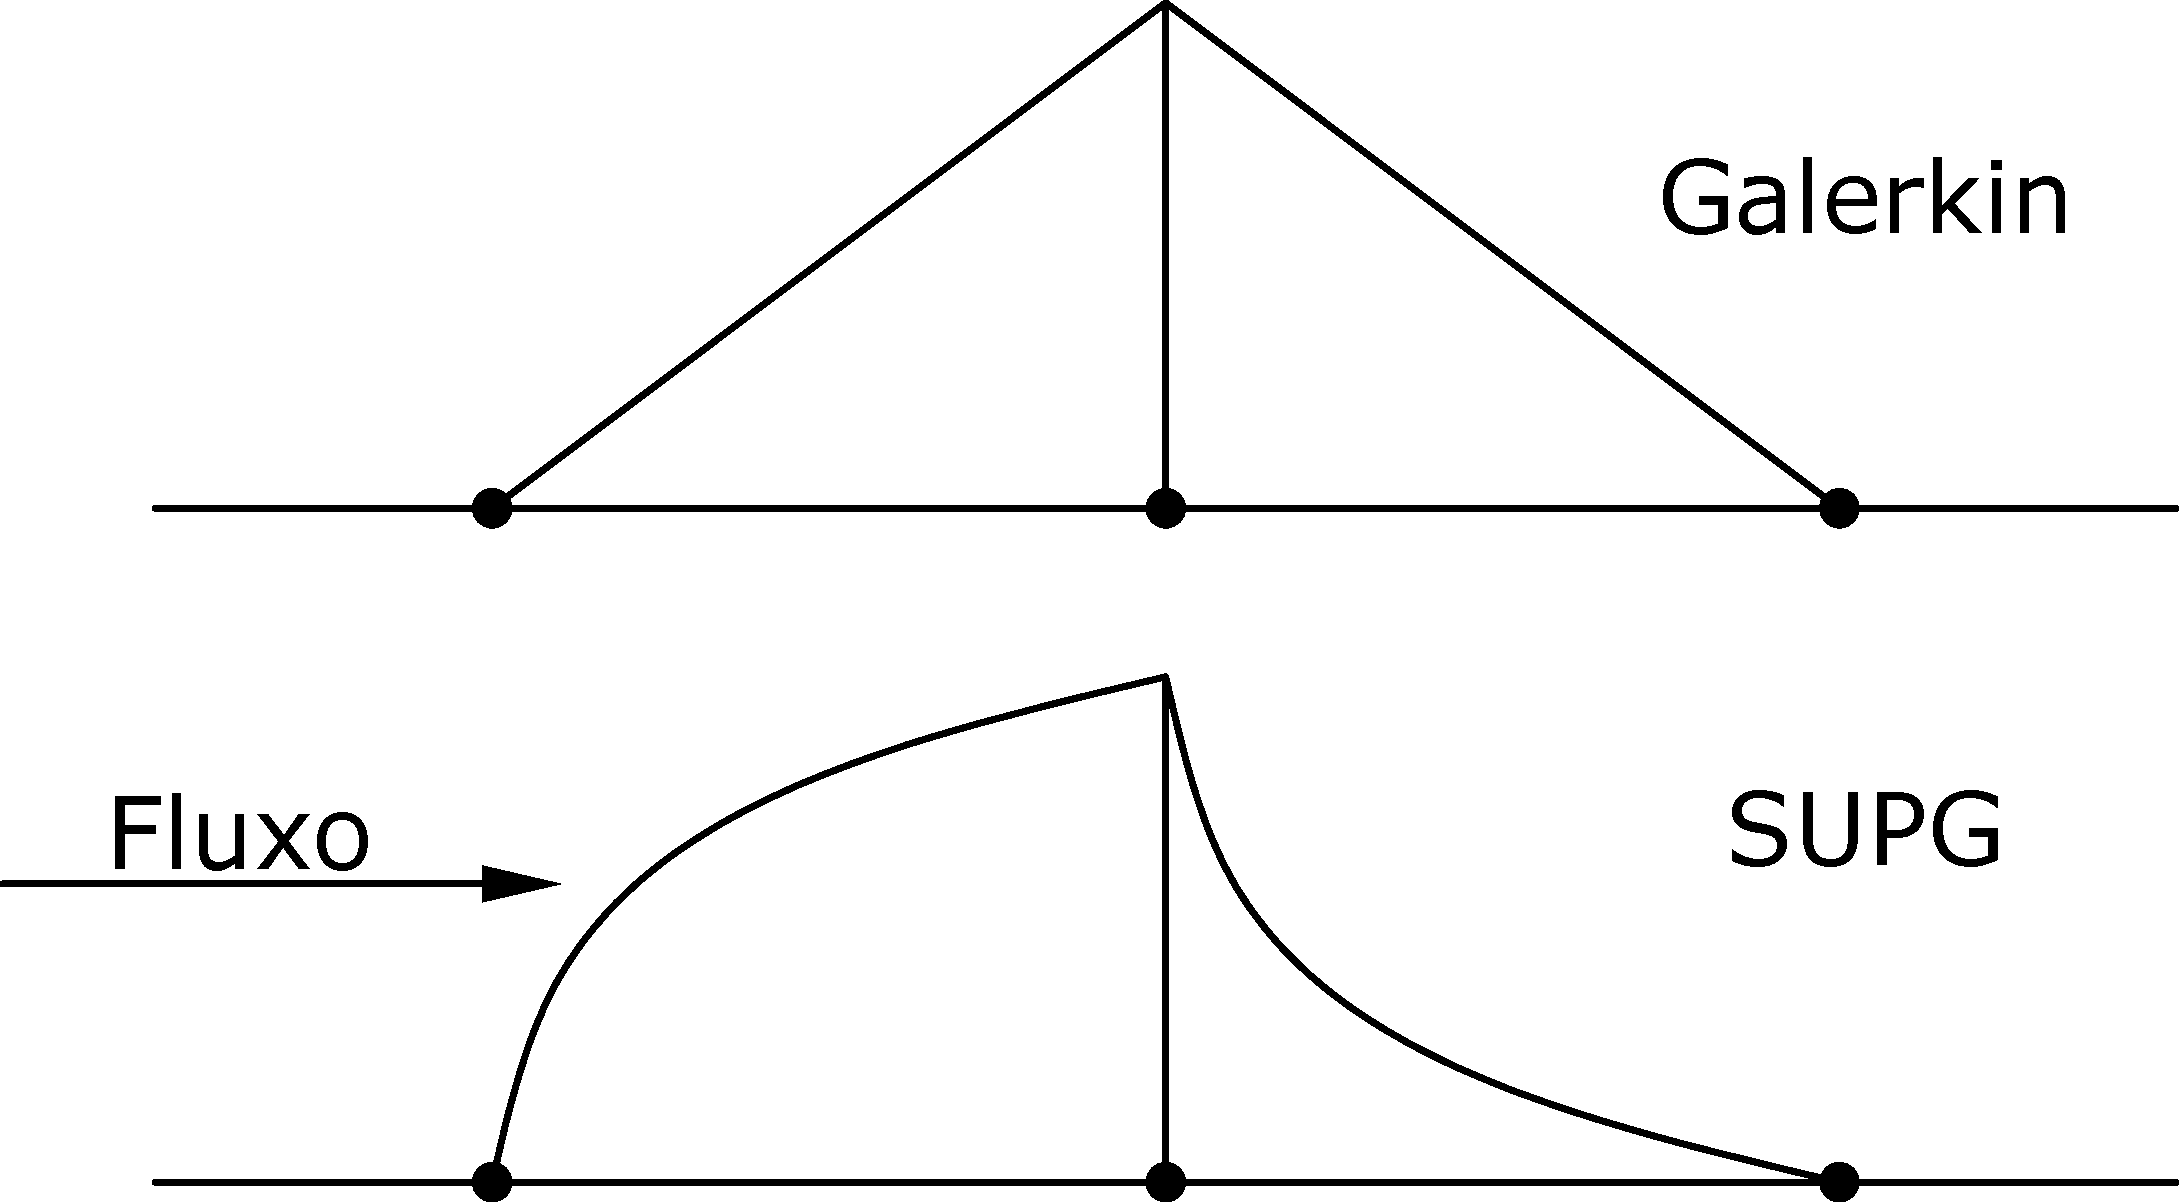
\includegraphics[width=.6\linewidth]{Figuras/SUPG.pdf}
    \\Fonte: \citeonline{brooks1982streamline} - Adaptado.
    \label{fig:Supg}
\end{figure}

Dessa forma surgirá um termo estabilizador que, multiplicado pelo resíduo da equação da conservação da quantidade de movimento, será capaz de reduzir as oscilações espúrias devido aos termos convectivos sem comprometer a previsão da solução.

%==================================================================================================
\subsection{Estabilização do campo de pressão}
%==================================================================================================

No intuito de se flexibilizar a escolha dos espaços aproximadores para pressão e velocidades, \citeonline{tezduyar1991stabilized} propuseram um método de estabilização que, de forma muito semelhante ao SUPG, multiplica o resíduo da equação da conservação da quantidade de movimento por um termo estabilizador. Nesse sentido, a estabilização PSPG preenche o sub-bloco nulo da matriz do sistema algébrico, melhorando tanto o condicionamento do sistema, como estabiliza o campo de pressões, permitindo também o uso de mesmos espaços aproximadores tanto para o campo de velocidades quanto de pressões.

%==================================================================================================
\subsection{Formulação Variacional Multiescala}
%==================================================================================================

%==================================================================================================
\section{\textit{Variational Multi-Scale}} \label{VMS}
%==================================================================================================

O Método Variacional Multiescala, introduzido por \citeonline{hughes1995multiscale,hughes1998variational,hughes2000large}, é um modelo de estabilização multiescala o qual faz a separação dos espaços de tentativas e de testes em subespaços que representem as escalas grosseiras, que se tratam de subespaços de dimensões finitas e denotadas por uma barra, e as escalas finas, que são subespaços de infinitas dimensões e denotadas por $'$, ou seja:

\begin{subequations}
    \begin{align}
         & \script{S}_u=\bar{\script{S}}_u\oplus\script{S}'_u\text{,}  \\
         & \script{S}_p=\bar{\script{S}}_p\oplus\script{S}'_p\text{,}  \\
         & \script{V}_u=\bar{\script{V}}_u\oplus\script{V}'_u\text{ e} \\
         & \script{V}_p=\bar{\script{V}}_p\oplus\script{V}'_p\text{.}
    \end{align}
\end{subequations}

Inicialmente será abordado uma técnica baseada em uma descrição Euleriana com domínio fixo, para maior familiarização com o método, e na sequência será apresentada uma formulação em descrição ALE utilizando domínio móvel.

O sistema a ser resolvido parte do apresentado em \ref{eq:NS-Euler}, que em sua forma fraca se encontra em \ref{eq:WeakForm2}. Primeiramente realiza-se a separação dos membros em:

\begin{subequations}
    \begin{align}
         & u_i=\bar{u}_i+u'_i\text{,}  \\
         & p=\bar{p}+p'\text{,}        \\
         & w_i=\bar{w}_i+w'_i\text{ e} \\
         & q=\bar{q}+q'\text{,}
    \end{align}
\end{subequations}

\noindent em que se adota $w_i=\bar{w}_i$ e $q=\bar{q}$ e as escalas finas $u'_i$ e $p'$ podem ser modeladas como:

\begin{subequations}
    \begin{equation}
        \BB{u}'=-\frac{\tau_{\sups}}{\rho}\rM\text{ e}
    \end{equation}
    \begin{equation}
        p'=-\rho\nu_{\lsic}\rC\text{,}
    \end{equation}
\end{subequations}

\noindent nas quais $\tau_{\sups}$ e $\nu_{\lsic}$ são termos estabilizadores, dados por \cite{bazilevs2013computational}:
%página 80 do pdf de hughes2013 e 65 de fernandes2020

\begin{subequations}
    \begin{equation}
        \tau_{\sups}=\bigpar{\frac{4}{\Delta t^2}+\BBB{u}\cdot\BB{G}\BBB{u}+C_I\nu^2\BB{G}:\BB{G}}^{-1/2}\text{ e}
    \end{equation}
    \begin{equation}
        \nu_{\lsic}=(\tr{\BB{G}}\tau_{\sups})^{-1}\text{,}
    \end{equation}
    \label{eq:TermEstab}
\end{subequations}

\noindent onde $C_I$ é uma constante e:

\begin{equation}
    \BB{G}=\frac{\partial\BB{\xi}}{\partial\BB{y}}^T\frac{\partial\BB{\xi}}{\partial\BB{y}}\text{.}
\end{equation}

Já os termos $\rMi{i}$ e $\rCi$ são os resíduos associados à equação de conservação da quantidade de movimento e da continuidade, respectivamente:

\begin{subequations}
    \begin{equation}
        \rMi{i}=\rho\bigpar{\dot{\bar{u}}_i+\bar{u}_j\bar{u}_{i,j}-\bar{f}_i}-\sigma_{ji,j}\text{ e}
    \end{equation}
    \begin{equation}
        \rCi=\bar{u}_{i,i}\text{.}
    \end{equation}
\end{subequations}

Outra forma de se modelar os termos estabilizadores pode ser dado por \cite{bazilevs2013computational}:

\begin{subequations}
    \begin{equation}
        \tau_{\sups}=\bigpar{\frac{1}{\tau_{\sugn 1}^2}+\frac{1}{\tau_{\sugn 2}^2}+\frac{1}{\tau_{\sugn 3}^2}}^{-1/2}\text{ e}
    \end{equation}
    \begin{equation}
        \nu_{\lsic}=\tau_{\sups}\norm{\BBB{u}}^2\text{,}
    \end{equation}
\end{subequations}

\noindent tal que:

\begin{subequations}
    \begin{align}
         & \tau_{\sugn 1}=\bigpar{\sum_{a=1}^{n_{en}}{\abs{\BBB{u}\cdot\NN N_a}}}^{-1}\text{,} \\
         & \tau_{\sugn 2}=\frac{\Delta t}{2}\text{,}                                           \\
         & \tau_{\sugn 3}=\frac{h_{\rgn}^2}{4\nu}\text{,}                                      \\
         & h_\rgn=2\bigpar{\sum_{a=1}^{n_{en}}{\abs{\BB{r}\cdot\NN N_a}}}^{-1}\text{ e}        \\
         & \BB{r}=\frac{\NN\norm{\BBB{u}}}{\norm{\NN\norm{\BBB{u}}}}\text{.}
    \end{align}
\end{subequations}

Assim, obtém-se o problema do Método Variacional Multiescala Baseado em Resíduos (\textit{Residual-Based Variational Multi-Scale} - RBVMS) que busca determinar $\BBB{u}\in\bar{\script{S}}_u$ e $\bar{p}\in\bar{\script{S}}_p$, tais que para todo $\BBB{w}\in\bar{\script{V}}_u$ e $\bar{q}\in\bar{\script{V}}_p$ \cite{bazilevs2013computational}:

\begin{equation}
    \begin{split}
        &\intDom{\bar{w}_i\rho\bigpar{\dot{\bar{u}}_i+\bar{u}_j\bar{u}_{i,j}-\bar{f}_i}}+\intDom{\bar{w}_{i,j}\bar{\sigma}_{ij}}-\intNeumann{\bar{w}_i\bar{h}_i}+\intDom{\bar{q}\bar{u}_{i,i}}-\\
        &\SintDom{\rho\bigpar{\bar{u}_j\bar{w}_{i,j}+\frac{\bar{q}_{,i}}{\rho}}u'_i}-\SintDom{\bar{w}_{i,i}p'}+\\
        &\SintDom{\rho\bar{w}_iu'_j\bar{u}_{i,j}}-\SintDom{\rho\bar{w}_{i,j}u'_iu'_j}=0
        \text{.}
        \label{eq:RBVMS1}
    \end{split}
\end{equation}

Para a discretização do problema pode-se realizar a separação da dependência espacial e temporal para os espaços tentativas e testes como:

\begin{subequations}
    \begin{align}
         & \bar{u}_i(\BB{y},t)=\sum_{\BB{\eta}^s}{U_i^a(t)N_a(\BB{y})}\text{,}             \\
         & \bar{p}(\BB{y},t)=\sum_{\BB{\eta}^s}{P^a(t)N_a(\BB{y})}\text{,}                 \\
         & \bar{w}_i(\BB{y})=\sum_{\BB{\eta}^w}{W_i^aN_a(\BB{y})}\text{ e}\label{eq:w-sep} \\
         & \bar{q}(\BB{y})=\sum_{\BB{\eta}^w}{Q^aN_a(\BB{y})}\text{.}\label{eq:q-sep}
    \end{align}
\end{subequations}

Substituindo \ref{eq:w-sep} e \ref{eq:q-sep} em \ref{eq:RBVMS1}, tais que $W^a$ e $Q^a$ são valores arbitrários, obtém-se dois vetores ($\NM=[(N_\mathrm{M})_i^a]$ e $\NC=[(N_\mathrm{C})^a]$) que representam resíduos a serem minimizados:

\begin{subequations}
    \begin{equation}
        \begin{split}
            (N_\mathrm{M})_i^a=&
            \intDom{N_a\rho\bigpar{\dot{\bar{u}}_i+\bar{u}_j\bar{u}_{i,j}-\bar{f}_i}}+\intDom{N_{a,j}\bar{\sigma}_{ij}}-\intNeumann{N_a\bar{h}_i}-\\
            &\SintDom{\rho N_{a,j}\bar{u}_ju'_i}-\SintDom{N_{a,i}p'}+\\
            &\SintDom{\rho N_a\bar{u}_{i,j}u'_j}-\SintDom{\rho N_{a,j}u'_iu'_j}
            \text{,}
        \end{split}
    \end{equation}
    \begin{equation}
        (N_\mathrm{C})^a=\intDom{N_a\bar{u}_{i,i}}-\SintDom{N_{a,i}u'_i}
    \end{equation}
    \label{Eq:Residuos-Euler}
\end{subequations}

Sendo os vetores $\BB{U}=[\BB{u}_B]$, $\dot{\BB{U}}=[\dot{\BB{u}}_B]$ e $\BB{P}=[p_B]$, que representam, respectivamente, os graus de liberdade em velocidades, primeira derivada temporal das velocidades e pressões nodais, então o problema a ser resolvido será dado por: encontrar $\BB{U}$, $\dot{\BB{U}}$ e $\BB{P}$, tais que:

\begin{subequations}
    \begin{align}
         & \NM(\BB{U},\dot{\BB{U}},\BB{P})=\BB{0}\text{ e} \\
         & \NC(\BB{U},\dot{\BB{U}},\BB{P})=\BB{0}\text{.}
    \end{align}
\end{subequations}

Uma formulação alternativa à apresentada é apresentada por \citeonline{bazilevs2013computational}, denominada como SUPG/PSPG, onde se omite os dois últimos termos da equação \ref{eq:RBVMS1} e se utiliza de valores diferentes de $\tau$ para as equações de conservação da quantidade de movimento e da continuidade, resultando em:

\begin{equation}
    \begin{split}
        &\intDom{\bar{w}_i\rho\bigpar{\dot{\bar{u}}_i+\bar{u}_j\bar{u}_{i,j}-\bar{f}_i}}+\intDom{\bar{w}_{i,j}\bar{\sigma}_{ij}}-\intNeumann{\bar{w}_i\bar{h}_i}+\intDom{\bar{q}\bar{u}_{i,i}}-\\
        &\SintDom{\tau_\supg\bar{w}_{i,j}\bar{u}_j\rMi{i}}-\SintDom{\tau_\pspg\frac{q_{,i}}{\rho}\rMi{i}}-\\
        &\SintDom{\rho\nu_\lsic\bar{w}_{i,i}\rCi}=0
        \text{,}
        \label{eq:SUPG-PSPG}
    \end{split}
\end{equation}

\noindent na qual, segundo os autores, adota-se $\tau_\pspg=\tau_\supg=\tau_\sups$ para uma boa variedade de problemas.

Por sua vez, a formulação baseada em uma descrição ALE parte das equações apresentadas em \ref{eq:NS-ALE}, cujo problema semi-discreto pode ser dado por:

\begin{equation}
    \begin{split}
        &\intDom{w_i\rho\bigpar{\dot{u}_i+(u_j-\hat{u}_j)u_{i,j}-f_j}}+\intDom{w_{i,j}\sigma_{ij}}-\\
        &\intNeumann{w_ih_i}+\intDom{qu_{i,i}}=0
    \end{split}
\end{equation}

Portanto o problema semi-discreto em formulação RBVMS de escoamentos incompressíveis segundo uma descrição ALE será: encontrar $\BBB{u}\in\bar{\script{S}}_u$ e $\bar{p}\in\bar{\script{S}}_p$, tais que para todo $\BBB{w}\in\bar{\script{V}}_u$ e $\bar{q}\in\bar{\script{V}}_p$ \cite{bazilevs2013computational}:

\begin{equation}
    \begin{split}
        &\intDom{\bar{w}_i\rho\bigpar{\dot{\bar{u}}_i+(\bar{u}_j-\hat{u}_j)\bar{u}_{i,j}-\bar{f}_i}}+\intDom{\bar{w}_{i,j}\bar{\sigma}_{ij}}-\intNeumann{\bar{w}_i\bar{h}_i}+\intDom{\bar{q}\bar{u}_{i,i}}-\\
        &\SintDom{\bigpar{\rho(\bar{u}_j-\hat{u}_j)\bar{w}_{i,j}+\bar{q}_{,i}}u'_i}-\SintDom{\bar{w}_{i,i}p'}+\\
        &\SintDom{\rho\bar{w}_i\bar{u}_{i,j}u'_j}-\SintDom{\rho\bar{w}_{i,j}u'_iu'_j}=0
        \text{,}
        \label{eq:RBVMS-ALE}
    \end{split}
\end{equation}

\noindent em que os termos estabilizadores $\tau_\sups$ e $\nu_\lsic$ são alterados das equações \ref{eq:TermEstab}, onde se considera, ao invés da velocidade do fluido $\bar{u}_i$, a velocidade relativa à malha ($\bar{u}_i-\hat{u}_i$), ou seja, $\bar{u}_i\gets\bar{u}_i-\hat{u}_i$.

Para o problema discretizado utiliza-se as seguintes expressões de aproximação dos espaços tentativas e testes:

\begin{subequations}
    \begin{align}
         & \bar{u}_i(\BB{y},t)=\sum_{\BB{\eta}^s}{U_i^a(t)N_a(\BB{y},t)}\text{,} \\
         & \bar{p}(\BB{y},t)=\sum_{\BB{\eta}^s}{P^a(t)N_a(\BB{y},t)}\text{,}     \\
         & \bar{w}_i(\BB{y})=\sum_{\BB{\eta}^w}{W_i^aN_a(\BB{y},t)}\text{ e}     \\
         & \bar{q}(\BB{y})=\sum_{\BB{\eta}^w}{Q^aN_a(\BB{y},t)}\text{,}
    \end{align}
\end{subequations}

\noindent onde as funções de forma $N_a(\BB{y},t)$ são definidas como:

\begin{equation}
    N_a(\BB{y},t)=\hat{N}_a(\bhat{f}^{-1}(\BB{y},t))\text{,}
\end{equation}

\noindent em que $\bhat{f}(\BB{y},t)$ é a função de mudança de configuração de $\hat{\Omega}\to\Omega$, conforme apresentado no item \ref{CFD-ALE}, dada em sua forma discreta por:

\begin{equation}
    \bhat{f}(\bhat{x},t)=\sum_{a\in\BB{\eta}^s}{(\bhat{x}_a+\Delta\bhat{x}_a(t))\hat{N}_a(\bhat{x})}\text{,}
\end{equation}

\noindent sendo $\bhat{x}_a$ as posições nodais em $\hat{\Omega}$, $\Delta\bhat{x}(t)$ o deslocamento nodal e $\hat{N}_a$ é a função de forma fixa da discretização de $\hat{\Omega}$. Nota-se, portanto, que as funções $N_a(\BB{y},t)$ possuem dependência temporal devido à movimentação da malha.

Com isso, define-se os vetores de resíduos da conservação de quantidade de movimento de da continuidade como:

\begin{subequations}
    \begin{equation}
        \NM=[(N_\mathrm{M})_i^a]\text{,}
    \end{equation}
    \begin{equation}
        \NC=[(N_\mathrm{C})^a]\text{,}
    \end{equation}
    \begin{equation}
        \begin{split}
            (N_\mathrm{M})_i^a=&
            \intDom{N_a\rho\bigpar{\dot{\bar{u}}_i+(\bar{u}_j-\hat{u}_j)\bar{u}_{i,j}-\bar{f}_i}}+\intDom{N_{a,j}\bar{\sigma}_{ij}}-\intNeumann{N_a\bar{h}_i}-\\
            &\SintDom{\rho N_{a,j}(\bar{u}_j-\hat{u}_j)u'_i}-\SintDom{N_{a,i}p'}+\\
            &\SintDom{\rho N_a\bar{u}_{i,j}u'_j}-\SintDom{\rho N_{a,j}u'_iu'_j}
            \text{,}
        \end{split}
    \end{equation}
    \begin{equation}
        (N_\mathrm{C})^a=\intDom{N_a\bar{u}_{i,i}}-\SintDom{N_{a,i}u'_i}
    \end{equation}
    \label{Eq:Residuos-ALE}
\end{subequations}

Assim, pretende-se determinar os vetores $\BB{U}$, $\dot{\BB{U}}$ e $\BB{P}$, tais que:

\begin{subequations}
    \begin{align}
         & \NM(\BB{U},\dot{\BB{U}},\BB{P})=\BB{0}\text{ e} \\
         & \NC(\BB{U},\dot{\BB{U}},\BB{P})=\BB{0}\text{.}
    \end{align}
\end{subequations}

%==================================================================================================
\subsection{Integração temporal} \label{IT-VMS}
%==================================================================================================

Como pôde-se verificar, em ambas as descrições, Euleriana e ALE, chega-se a um problema discreto no espaço, porém contínuo no tempo (Equações \ref{Eq:Residuos-Euler} e \ref{Eq:Residuos-ALE}). Dessa forma torna-se necessária a devida discretização temporal das variáveis, que pode ocorrer de diferentes formas, como apontado por \citeonline{reddy2010finite}, tem-se, por exemplo, o surgimento de integradores explícitos, como o integrador baseado em diferenças adiantadas, implícitos, como em diferenças finitas atrasadas, e o denominado semi-explícito (ou da regra de trapézios). Segundo o autor os integradores implícitos possuem vantagens sobre os explícitos, uma vez que: se observa a implicidade natural da pressão em escoamentos incompressíveis; deve-se ter um cuidado extra para garantir a estabilidade do integrador; apresentar problemas para a diagonalização de matrizes de massa; e perda de precisão na diagonalização.

O integrador temporal utilizado no presente trabalho é o denominado integrador $\alpha$-generalizado, desenvolvido por \citeonline{chung1993time}, que possui a capacidade de representar adequadamente problema de escoamentos incompressíveis, além de permitir a introdução de difusão numérica ao processo \cite{fernandes2020tecnica}.

Esse integrador parte da consideração de valores intermediários de aceleração e velocidade em um intervalo de tempo $[t_n,t_{n+1}]$ no $n$-ésimo passo de tempo, representados respectivamente por $\dot{\BB{U}}^{n+\alpha_m}$ e $\BB{U}^{n+\alpha_f}$:

\begin{subequations}
    \begin{equation}
        \dot{\BB{U}}^{n+\alpha_m}=\dot{\BB{U}}^n+\alpha_m(\dot{\BB{U}}^{n+1}-\dot{\BB{U}}^n)\text{ e}
    \end{equation}
    \begin{equation}
        \BB{U}^{n+\alpha_f}=\BB{U}^n+\alpha_f(\BB{U}^{n+1}-\BB{U}^n)\text{.}
    \end{equation}
\end{subequations}

Já para se relacionar a velocidade à aceleração, pode-se proceder com a aproximação de Newmark \cite{bazilevs2013computational}:

\begin{equation}
    \BB{U}^{n+1}=\BB{U}^n+\Delta t_n\bigpar{(1-\gamma)\dot{\BB{U}}^n+\gamma\dot{\BB{U}}^{n+1}}\text{,}
\end{equation}

\noindent sendo $\alpha_m$, $\alpha_f$ e $\gamma$ valores escolhidos arbitrariamente observando as necessidades de estabilidade e precisão do método.

De acordo com \citeonline{chung1993time,jansen2000generalized,bazilevs2013computational}, a precisão de segunda ordem dessa aproximação pode ser atingida uma vez que:

\begin{equation}
    \gamma=\frac{1}{2}+\alpha_m-\alpha_f\text{,}
\end{equation}

\noindent enquanto a estabilidade incondicional pode ser obtida caso:

\begin{equation}
    \alpha_m\geq\alpha_f\geq\frac{1}{2}\text{.}
\end{equation}

Ainda é possível escrever, a partir da Equação \ref{eq:one-par-stable}, $\alpha_m$ e $\alpha_f$ em termos de um parâmetro arbitrário único  ($0\leq\rho_\infty\leq1$), que representa o raio espectral de amplificação da matriz para $\Delta t\to\infty$, o qual é utilizado para controlar as dissipações de alta-frequência.

\begin{subequations}
    \begin{equation}
        \alpha_m=\frac{1}{2}\bigpar{\frac{3-\rho_\infty}{1+\rho_\infty}}\text{ e}
    \end{equation}
    \begin{equation}
        \alpha_f=\frac{1}{1+\rho_\infty}\text{.}
    \end{equation}
    \label{eq:one-par-stable}
\end{subequations}

Para o caso de $\rho_\infty=1$ não ocorre a introdução de difusão numérica, enquanto para $\rho_\infty=0$ se tem a máxima dissipação de altas frequências \cite{fernandes2020tecnica}.

Sendo assim, os resíduos obtidos anteriormente podem ser escritos em termos dos valores intermediários como:

\begin{subequations}
    \begin{equation}
        \NM(\dot{\BB{U}}^{n+\alpha_m},\BB{U}^{n+\alpha_f},\BB{P}^{n+1})=0
    \end{equation}
    \begin{equation}
        \NC(\dot{\BB{U}}^{n+\alpha_m},\BB{U}^{n+\alpha_f},\BB{P}^{n+1})=0
    \end{equation}
\end{subequations}

%%==================================================================================================
%\subsection{Procedimento iterativo} \label{Comp-VMS}
%%==================================================================================================
%
%O procedimento para minimizar os vetores resíduo obtido parte do método de Newton-Raphson, no qual os valores a serem corrigidos são os vetores de acelerações nodais ($\dot{\BB{U}}$) e de pressões nodais ($\BB{P}$). Dessa forma, o problema a ser resolvido para a correção dessas variáveis é:
%
%\begin{equation}
%    \begin{bmatrix}
%        \der{(N_M)_i^a}{(\dot{U}_j^b)^{n+1}} & \der{(N_M)_i^a}{(P^b)^{n+1}} \\
%        \der{(N_C)^a}{(\dot{U}_j^b)^{n+1}}   & \der{(N_C)^a}{(P^b)^{n+1}}
%    \end{bmatrix}
%    \begin{bmatrix}
%        \Delta(\dot{U}_j^b)^{n+1} \\
%        \Delta (P^b)^{n+1}
%    \end{bmatrix}=-
%    \begin{bmatrix}
%        (N_M)_i^a \\
%        (N_C)^a
%    \end{bmatrix}\text{,}
%    \label{Eq:Newton-Raphson}
%\end{equation}
%
%\noindent em que, para uma descrição ALE:
%
%\begin{subequations}
%    \begin{equation}
%        \begin{split}
%            \der{(N_M)_i^a}{(\dot{U}_j^b)^{n+1}}=&\am\intDomna{\rho N_aN_b}\dij+\am\intDomna{\rho\tsups N_{a,k}N_{b}\uub{k}}\dij+\\
%            &\agdt\intDomna{\rho N_aN_{b,k}\uub{k}}\dij+\agdt\intDomna{\mu N_{a,k}N_{b,k}}\dij+\\
%            &\agdt\intDomna{\mu N_{a,j}N_{b,i}}+\agdt\intDomna{\rho\nlsic N_{a,i}N_{b,j}}+\\
%            &\agdt\intDomna{\rho\tsups N_{a,k}N_{b,m}\uub{k}\uub{m}}\dij+\\
%            &\agdt\intDomna{\rho N_aN_b\bar{u}_{i,j}}+\agdt\intDomna{\rho\tsups N_{a,k}N_b\uub{k}\bar{u}_{i,j}}-\\
%            &\am\intDomna{\rho\tsups N_aN_b\bar{u}_{i,j}}-\\
%            &\agdt\intDomna{\rho\tsups N_aN_{b,m}\uub{m}\bar{u}_{i,j}}-\\
%            &\agdt\intDomna{\rho\tsups N_aN_b\bar{u}_{i,k}\bar{u}_{k,j}}\text{,}
%        \end{split}
%    \end{equation}
%    \begin{equation}
%        \begin{split}
%            \der{(N_M)_i^a}{(P^b)^{n+1}}=&-\intDomna{N_{a,i}N_b}+\intDomna{\tsups N_{a,j}N_{b,i}\uub{j}}-\\
%            &\intDomna{\tsups N_aN_{b,j}\bar{u}_{i,j}}\text{,}
%        \end{split}
%    \end{equation}
%    \begin{equation}
%        \begin{split}
%            \der{(N_C)^a}{(\dot{U}_j^b)^{n+1}}=&\agdt\intDomna{N_aN_{b,j}}+\am\intDomna{\tsups N_{a,j}N_b}+\\
%            &\agdt\intDomna{\tsups N_{a,j}N_{b,m}\uub{m}}+\\
%            &\agdt\intDomna{\tsups N_{a,i}N_b\bar{u}_{i,j}}\text{ e}
%        \end{split}
%    \end{equation}
%    \begin{equation}
%        \der{(N_C)^a}{(P^b)^{n+1}}=\intDomna{\frac{\tsups}{\rho}N_{a,i}N_{b,i}}\text{,}
%    \end{equation}
%\end{subequations}
%
%\noindent em que $\agdt=\alpha_f\gamma\Delta t$ e:
%
%\begin{equation}
%    \Omega^{n+\alpha_f}=\left\{\bar{\BB{x}}|\bar{\BB{x}}(\hat{\BB{x}},t^{n+\alpha_f})=\alpha_f\bar{\BB{x}}(\hat{\BB{x}},t^{n+1})+(1-\alpha_f)\bar{\BB{x}}(\hat{\BB{x}},t^n)\right\}\text{.}
%\end{equation}
%
%Para uma descrição Euleriana, considera-se a velocidade da malha como nula na formulação apresentada.
%
%Sendo assim, o pseudocódigo apresentado no algoritmo presente no Apêndice \ref{Ap:MEF-VMS} mostra o procedimento para obtenção da solução aproximada.

%==================================================================================================
%==================================================================================================
\subsection{\textit{Large Eddy Simulation}} \label{LES}
%==================================================================================================

Em escoamentos com elevados números de Reynolds, observa-se a formação de vórtices em um amplo espectro de escalas, o que torna a simulação direta desses escoamentos computacionalmente inviável, uma vez que se exigem altas resoluções da malha do fluido para capturar todos os efeitos. Nesse sentido, a simulação de grandes vórtices (\textit{Large Eddy Simulation} - LES) surge como uma alternativa para se obter resultados próximos aos da simulação direta, porém com um custo computacional reduzido.

O LES originou-se do trabalho de \citeonline{smagorinsky1963general} no intuito de se estudar simulações de camadas limite atmosféricas e tendo o coeficiente de Smagorinsky estimado por \citeonline{deardorff1971magnitude} ao estudar escoamentos em canais. A ideia central do modelo parte da consideração de que o escoamento pode ser bem caracterizado por meio de uma separação de escalas, na qual as grandes escalas são responsáveis pela transferência da energia cinética, sendo influenciadas diretamente pela natureza do escoamento, assim como pelas condições de contorno, enquanto as pequenas escalas são responsáveis pela dissipação de energia e possuem propriedades isotrópicas e homogêneas no escoamento. Assim, o modelo de Smagorinsky consiste em uma decomposição do campo de velocidades em duas parcelas, uma de grandes escalas e outra de pequenas escalas, sendo a parcela de pequenas escalas modelada por um termo viscoso, o qual é determinado a partir de um modelo de viscosidade de vórtice.

Assim, a decomposição das variáveis do problema ($\phi$) se dá por $\phi=\bar{\phi}+\phi'$, em que $\bar{\phi}$ é a parcela de grandes escalas e $\phi'$ é a parcela de pequenas escalas. Tal separação é dada a partir da consideração de um filtro, definido como a convolução integral de uma função $\filter$, dita como filtro, com a variável $\phi$ \cite{germano1991dynamic,hughes2000large,moeng2015large,katopodes2019free}:

\begin{equation}
    \bar{\phi}=\int_{\Dfil}{\filter(\BB{y}-\yfil,t)\phi(\yfil,t)d\yfil}\text{,}
\end{equation}

\noindent em que $\Dfil$ é um subdomínio de $\Omega$ que determina a abrangência do filtro, $\yfil$ é um ponto na vizinhança de $\BB{y}$ e $\filter$ é o filtro. \citeonline{hughes2000large} apresentam ainda uma possibilidade de abrangência de filtro dada por:

\begin{equation}
    \Dfil=\left\{\yfil\in\mathbb{R}^{n_{sd}}|\rho_\Delta(\BB{y},\yfil)<\Delta/2\right\}\text{,}
\end{equation}

\noindent na qual $\Delta/2$ é o raio de abrangência do filtro centrado em $\BB{y}$ e $\rho_\Delta$ é a distância Euclidiana de $\yfil$ à $\BB{y}$.

Assim, um filtro $\filter$ deve ser capaz de remover as altas frequências na representação de Fourier e deve ser escolhido de forma a obedecer algumas propriedades, \ie\ a condição de homogeneidade: $\filter(\BB{y},\yfil,t)=\filter(\BB{y}-\yfil,t)$, a condição de isotropia: $\filter(\BB{y}-\yfil,t)=\filter(\rho_\Delta,t)$, a condição de normalização:

\begin{equation}
    \int_{\Dfil}{\filter(\BB{y}-\yfil,t)d\yfil}=1
\end{equation}

\noindent e deve possuir um suporte compacto, ou seja, sua influência deve diminuir com o aumento da distância de seu centro.

Dessa maneira, algumas propriedades são garantidas, como a conversão da operação de convolução em multiplicação em um espaço de Fourier, a qual é dada por:

\begin{subequations}
    \begin{equation}
        \Fourier{\bar{\phi}}(\BB{k},t)=\Fourier{\filter}(\BB{k},t)\Fourier{\phi}(\BB{k},t)\text{ e}
    \end{equation}
    \begin{equation}
        \Fourier{\phi'}(\BB{k},t)=(1-\Fourier{\filter}(\BB{k},t))\Fourier{\phi}(\BB{k},t)\text{,}
    \end{equation}
\end{subequations}

\noindent em que a variável $\BB{k}$ representa o número de onda e o sobrescrito $\mathcal{F}$ representa a transformação de Fourier. Além disso, a filtragem é uma operação linear, ou seja, $\bar{\phi_1+\phi_2}=\bar{\phi_1}+\bar{\phi_2}$ e $\bar{\alpha\phi}=\alpha\bar{\phi}$, em que $\alpha$ é uma constante. Já em domínios ilimitados, cujo filtro possui abrangência constante, tem-se a comutatividade da filtragem com a diferenciação, ou seja, $\bar{\Ny\phi}=\Ny\bar{\phi}$.

\citeonline{katopodes2019free} apresenta algumas possibilidades de filtro, os quais são apresentados na Tabela \ref{tab:filters}, assim como sua respectiva transformada de Fourier. A Figura \ref{fig:Filters} apresenta graficamente o comportamento dos filtros apresentados na Tabela \ref{tab:filters}.

\begin{table}[h!]
    \centering
    \caption{Filtros utilizados em \LES.}
    \begin{tabular}{lll}
        \hline
        Filtro              & Função                                                                                                                                             & Transformada de Fourier                                                                                                  \\\hline
        \textit{Box filter} & $\filter(\rho_\Delta)=\left\{\begin{array}{ll}\frac{1}{\Delta} & \text{ se }\rho_\Delta\leq\Delta/2 \\0& \text{ caso contrário}\end{array}\right.$ & $\Fourier{\filter}(k)=\frac{\sin{(k\Delta/2)}}{k\Delta/2}$                                                               \\
        Filtro gaussiano    & $\filter(\rho_\Delta)=\sqrt{\frac{\gamma_g}{\pi\Delta^2}}\exp{\left\{-\frac{\gamma\rho_\Delta^2}{\Delta^2}\right\}}$                               & $\Fourier{\filter}(k)=\exp{\left\{-\frac{k^2\Delta^2}{4\gamma}\right\}}$                                                 \\
        Filtro espectral    & $\filter(\rho_\Delta)=\frac{\sin{(k_c\rho_\Delta)}}{k_c\rho_\Delta}$                                                                               & $\Fourier{\filter}(k)=\left\{\begin{array}{ll} 1 & \text{ se }|k|\leq k_c \\0& \text{ caso contrário}\end{array}\right.$ \\\hline
    \end{tabular}
    \\Fonte: \citeonline{katopodes2019free} - Adaptado.
    \label{tab:filters}
\end{table}

\begin{figure}[h!]
    \centering
    \caption{Comportamento dos filtros apresentados na Tabela \ref{tab:filters}.}
    \begin{subfigure}{0.4\textwidth}
        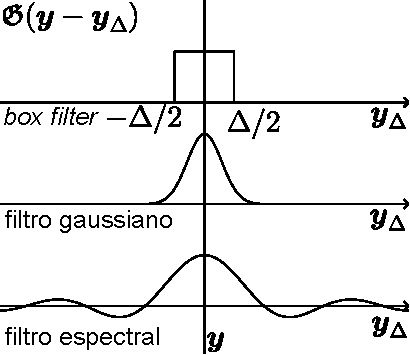
\includegraphics[width=\linewidth]{Figuras/filtros1.pdf}
        \caption{Função filtro.}
    \end{subfigure}
    \begin{subfigure}{0.4\textwidth}
        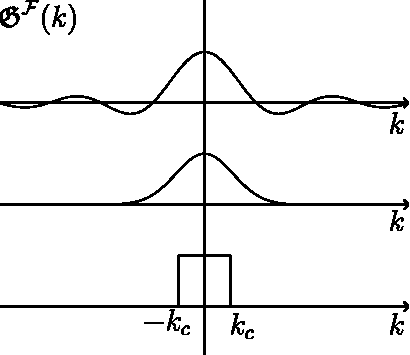
\includegraphics[width=\linewidth]{Figuras/filtros2.pdf}
        \caption{Transformada de Fourier.}
    \end{subfigure}
    \\Fonte: Autoria Própria (\the\year).
    \label{fig:Filters}
\end{figure}

O valor $\gamma_g$ observado no filtro gaussiano é uma constante, comumente atribuída com o valor de 6,0. Já o parâmetro $k_c$ é o número de onda de corte, dado por $k_c=\pi/\Delta$. Dentre os filtros apresentados, percebe-se que tanto o \textit{box filter} quanto o filtro gaussiano possuem suporte compacto no espaço físico, porém não possuem suporte compacto no espaço de Fourier, o que pode gerar problemas numéricos. Já o filtro espectral possui suporte compacto no espaço de Fourier, porém não possui suporte compacto no espaço físico.

Dessa maneira, é possível separar os efeitos das grandes escalas e das pequenas escalas, o que é ilustrado na Figura \ref{fig:EfeitoFiltragem} para uma distribuição de velocidade $\BB{u}$.

\begin{figure}[h!]
    \centering
    \caption{Efeito da filtragem sobre um campo de velocidades $\BB{u}$.}
    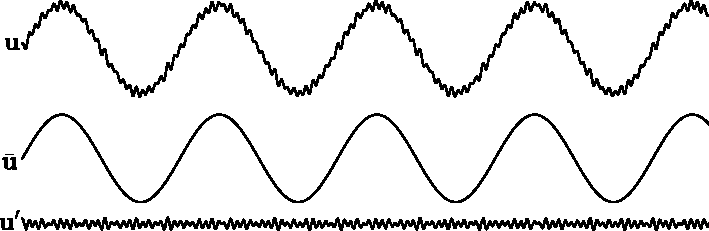
\includegraphics[width=.75\linewidth]{Figuras/efeito_filtragem.pdf}
    \\Fonte: \citeonline{hughes2000large} - Adaptado.
    \label{fig:EfeitoFiltragem}
\end{figure}

Assim, em uma descrição Euleriana, pode-se obter as equações de Navier-Stokes filtradas:

\begin{subequations}
    \begin{align}
         & \rho\bigpar{\dot{\BBB{u}}+\Ny\cdot(\overline{\BB{u}\otimes\BB{u}})-\BBB{f}}-\Ny\cdot\bar{\tens}=\BB{0} &  & \text{ em }\Omega\text{,} \\
         & \Ny\cdot\BBB{u}=0                                                                                      &  & \text{ em }\Omega\text{.}
    \end{align}
\end{subequations}

Pode-se perceber que o termo convectivo impede a completa separação dos termos $\BBB{u}$ e $\BB{u}'$ devido à sua natureza altamente não-linear. Por conta disso a parcela não filtrada não pode ser ignorada nesse problema, sendo necessário realizar algumas manipulações algébricas. Sabendo-se que $\BB{u}=\BBB{u}+\BB{u}'$, pode-se reescrever a equação da conservação da quantidade de movimento como:

\begin{equation}
    \rho\bigpar{\dot{\BBB{u}}+\Ny\cdot(\overline{(\BBB{u}+\BB{u}')\otimes(\BBB{u}+\BB{u}')})-\BBB{f}}-\Ny\cdot\bar{\tens}=\BB{0}
\end{equation}

Nesse sentido, surgirão termos cruzados entre $\BBB{u}$ e $\BB{u}'$, os quais serão condensados em um tensor de subescala (\textit{Subgrid-Scale} - SGS) $\BB{T}$ dado por \cite{piomelli1999large,hughes2000large}:

\begin{equation}
    \BB{T}=\BBB{u}\otimes\BBB{u}-\overline{\BB{u}\otimes\BB{u}}=-\bigpar{\BB{L}+\BB{C}+\BB{R}}\text{,}
\end{equation}

\noindent no qual $\BB{L}=\overline{\BBB{u}\otimes\BBB{u}}-\BBB{u}\otimes\BBB{u}$ é o tensor de Leonard, que representa as interações entre as grandes escalas, podendo ser determinado explicitamente e utilizado para análise de erros, $\BB{C}=\overline{\BBB{u}\otimes\BB{u}'}+\overline{\BB{u}'\otimes\BBB{u}}$ é o tensor de termos cruzados, representando a interação entre as grandes e pequenas escalas e $\BB{R}=\overline{\BB{u}'\otimes\BB{u}'}$ é o tensor de tensões SGS de Reynolds, que representa a interação entre as pequenas escalas \cite{piomelli1999large}. Assim pode-se escrever:

\begin{equation}
    \rho\bigpar{\dot{\BBB{u}}+\Ny\cdot(\BBB{u}\otimes\BBB{u})-\Ny\cdot\BB{T}-\BBB{f}}-\Ny\cdot\bar{\tens}=\BB{0}\text{.}
\end{equation}

Aplicando a incompressibilidade e substituindo-se $\bar{\tens}$ pelo modelo constitutivo \eqref{eq:ModConst}, tem-se que:

\begin{equation}
    \rho\bigpar{\dot{\BBB{u}}+(\BBB{u}\cdot\Ny)\BBB{u}-\Ny\cdot\BB{T}-\BBB{f}}-\mu\Ny\cdot(\Ny\BBB{u}+\NyT\BBB{u})+\Ny p=\BB{0}\text{,}\label{eq:ConMasLES}
\end{equation}

\noindent ou, dividindo-se por $\rho$ e fazendo algumas manipulações tem-se que:

\begin{equation}
    \dot{\BBB{u}}+(\BBB{u}\cdot\Ny)\BBB{u}+\frac{\Ny p}{\rho}=\nu\Lapl\BBB{u}+\Ny\BB{T}+\BBB{f}\text{,}
\end{equation}

\noindent sendo $\Lapl(\cdot)=\Ny\cdot\Ny(\cdot)$ o operador laplaciano e $\nu=\mu/\rho$ a viscosidade cinemática.

Assim, o problema fica governado por:

\begin{equation}
    \left\{
    \begin{array}{ll}
        \dot{\BBB{u}}+(\BBB{u}\cdot\Ny)\BBB{u}+\frac{\Ny p}{\rho}=\nu\Lapl\BBB{u}+\Ny\cdot\BB{T}+\BBB{f} & \text{ em }\Omega\text{,} \\
        \Ny\cdot\BBB{u}=0                                                                                & \text{ em }\Omega\text{,}
    \end{array}
    \right.
\end{equation}

\noindent havendo ainda a necessidade de se determinar um tensor $\BB{T}$, em especial o seu tensor desviador:

\begin{equation}
    \dev{\BB{T}}=\BB{T}-\frac{1}{3}\tr{(\BB{T})}\BB{I}\text{,}
\end{equation}

\noindent que descreva adequadamente as interações entre diferentes escalas. Isso pode se tornar problemático uma vez que não se possui solução para as pequenas escalas. Uma forma de se fazer isso é através do modelo de viscosidade de vórtice de Smagorinsky \cite{smagorinsky1963general}, resultando no tensor:

\begin{equation}
    \bigpar{\BB{T}_S}=2\nu_T\deffil\text{,}
\end{equation}

\noindent sendo $\nu_T$ a viscosidade de vórtice SGS, dada por \cite{germano1991dynamic,piomelli1999large,hughes2000large,bailly2015turbulence,katopodes2019free}:

\begin{equation}
    \nu_T=(C_S\Delta)^2\norm{\deffil}\text{,}
\end{equation}

\noindent onde $C_S$ é a constante de Smagorinsky e $\norm{\deffil}$ é a magnitude do tensor taxa de deformação em escala grosseira, dada por:

\begin{equation}
    \norm{\deffil}=(2\deffil:\deffil)^{1/2}\text{.}
\end{equation}

Note que o tensor $\BB{T}_S$ é um tensor desviador, ou seja, $\BB{T}_S=\dev{\BB{T}_S}$.

%\citeonline{germano1991dynamic,hughes2000large} ainda fazem algumas constatações sobre o modelo de Smagorinsky, os quais destacam-se o fato de $\BB{T}_S$ não possuir um comportamento assintótico próximo às paredes, o que se esperaria de $\BB{T}$, os valores de $C_S$ na presença de cisalhamento médio causaram amortecimentos excessivos e o tensor $\BB{T}_S$ impede a energia de fluir entre diferentes escalas, podendo ser significante em alguns casos.
%
%Como tentativa de se resolver esses problemas, \citeonline{germano1991dynamic} propuseram assumir $C_S$ como uma função $C_S=C_S(\BB{y},t)$, permitindo, assim, que esse parâmetro se adapte para melhor modelar as pequenas escalas.

Para a determinação da constante de Smagorinsky, realiza-se inicialmente uma aproximação da amplitude espectral da energia cinética $E(k)$, dada sobre a superfície de uma esfera parametrizada de raio $k$, de acordo com \cite{hughes2000large}:

\begin{equation}
    E(k)\approx\alpha\varepsilon^{2/3}k^{-5/3}\text{,}\label{eq:Ek1}
\end{equation}

\noindent em que $\alpha$ é a constante de Kolmogoroff e $\varepsilon$ é a dissipação turbulenta. A Figura \ref{fig:EnergiaEspectral} apresenta graficamente o comportamento da energia espectral em função de $k$.

\begin{figure}[h!]
    \centering
    \caption{Amplitude da energia espectral.}
    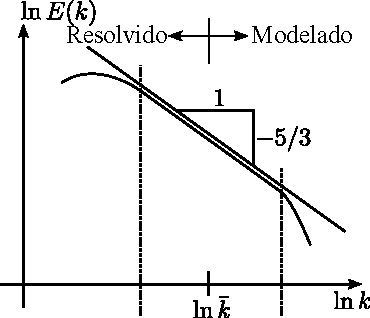
\includegraphics[width=0.4\linewidth]{Figuras/EnergiaEspectral.pdf}
    \\Fonte: \cite{hughes2000large} - Adaptado.
    \label{fig:EnergiaEspectral}
\end{figure}

O valor de $\norm{\deffil}$ é adotado como:

\begin{equation}
    \frac{1}{2}\norm{\deffil}=\int_0^{k_c}{k^2E(k)dk}\text{,}\label{eq:ndeffil1}
\end{equation}

\noindent sendo $k_c$ o limite de resolução.

Substituindo \eqref{eq:Ek1} em \eqref{eq:ndeffil1}, resolvendo a integral e fazendo algumas manipulações algébricas, tem-se que:

\begin{equation}
    \norm{\deffil}^3=\bigpar{\frac{3\alpha}{2}}^{3/2}k_c^2\varepsilon\text{.}
\end{equation}

Com isso, considerando também que a dissipação de energia cinética é igual àquela produzida, realiza-se o balanço da energia, obtendo-se:

\begin{equation}
    \varepsilon=\BB{T}_S:\deffil\text{.}
\end{equation}

\noindent Assim, fica possível obter expressões que relacionam os valores de $C_S$ $\Delta$ e $\nu_T$ com $k_c$:

\begin{equation}
    C_S\Delta=\bigpar{\frac{2}{3\alpha}}^{3/4}k_c^{-1}\text{ e}
\end{equation}

\begin{equation}
    \nu_T=\bigpar{\frac{2}{3\alpha}}\varepsilon^{1/3}k_c^{-4/3}\text{.}
\end{equation}

Segundo \citeonline{bailly2015turbulence} o valor de $k_c$ pode ser estimado como $k_c=\pi/\Delta$, o que leva à seguinte expressão para a constante de Smagorinsky:

\begin{equation}
    C_S=\frac{1}{\pi}\bigpar{\frac{2}{3\alpha}}^{3/4}\text{.}
\end{equation}

Com isso, um possível valor para a constante Kolmogoroff é $\alpha=1,4$, o que resulta em $C_S\approx0,18$. No entanto, segundo  \citeonline{hughes2000large,bailly2015turbulence,katopodes2019free}, valores de $C_S$ próximos à 0,10 conduzem a solução à resultados mais realistas.

\begin{comment}
%==================================================================================================
\subsubsection{Procedimento computacional} \label{LES-PC}
%==================================================================================================

Para a obtenção dos resultados, parte-se para a formulação variacional, em que se utiliza funções testes $\BB{w}$ e $q$, associadas às equações de conservação da quantidade de movimento e da continuidade, respectivamente. Assim, a forma fraca do problema LES é dada por:

\begin{equation}
    \begin{split}
        &\intDom{w_i\rho\bigpar{\dot{\ub}_i+\uub{j}\ub_{i,j}-\bar{f}_i}}+\intDom{\rho w_{i,j}T_{ij}}+\intDom{w_{i,j}\sigma_{ji}(\BB{\ub},\pb)}+\\
        &\intDom{q\ub_{i,i}}-\intNeumann{\rho w_iT_{ij}n_j}-\intNeumann{w_i\bar{h}_i}=0\text{.}
    \end{split}
\end{equation}

Substituindo o modelo constitutivo e o modelo de viscosidade de Smagorinsky tem-se que:

\begin{equation}
    \begin{split}
        &\intDom{w_i\rho\bigpar{\dot{\ub}_i+\uub{j}\ub_{i,j}-\bar{f}_i}}+\intDom{w_{i,j}(\mu+\rho\nu_T)(\uSim{\ub}{i}{j})}-\\
        &\intDom{w_{i,i}\pb}+\intDom{q\ub_{i,i}}-\intNeumann{w_i\bar{h}_i}=0\text{.}
    \end{split}
\end{equation}

\textcolor{purple}{
    No intuito de se obter uma solução estável, será considerado o elemento de Taylor-Hood P2P1 (aproximação quadrática para o campo de velocidades e linear para o campo de pressões) na formulação. Assim denomina-se $M$ as funções de forma para aproximação quadrática e $N$ para funções de forma lineares. Com isso, faz-se a aproximação das funções testes por meio das funções de forma, tendo como resultado os seguintes vetores de resíduo associados às equações de conservação de momento e da continuidade:
}
\textcolor{red}{1. Você deve deixar a formulação geral, e nos exemplos dizer o que você utilizou para obter resposta estável. Sugiro que desde o início (VMS) você diferencie as funções de forma de pressão e de velocidade (eu prefiro colocar um sobrescrito u e p ao invés de usar N e M). Aqui você deveria apresentar a formulação estabilizada, e nos exemplos você diz o que adotou para rodar. De qualquer forma, aqui ficou faltando colocar a estabilização para a convecção (SUPG) que sempre será necessária. Reveja o restante deste item com base nisso...}

\begin{subequations}
    \begin{equation}
        \begin{split}
            \bigpar{N_M}_i^a=&\intDom{M_a\rho\bigpar{\dot{\ub}_i+\uub{j}\ub_{i,j}-\bar{f}_i}}+\\
            &\intDom{M_{a,j}(\mu+\rho\nu_T)(\uSim{\ub}{i}{j})}-\intDom{M_{a,i}\pb}-\intNeumann{N_a\bar{h}_i}\text{ e}
        \end{split}
    \end{equation}
    \begin{equation}
        \bigpar{N_C}^a=\intDom{N_a\ub_{i,i}}\text{.}
    \end{equation}
    \label{eq:VetoresResiduo-LES}
\end{subequations}

Dessa forma procura-se determinar valores de $\ub$ e $\pb$ que anulem $N_M$ e $N_C$. Para esse fim utiliza-se o método de Newton-Raphson, em que as variáveis a serem determinadas são as acelerações e pressões nodais, sendo o integrador utilizado o $\alpha$-generalizado, apresentado na seção \ref{IT-VMS}. Desse modo tem-se os seguintes sub-blocos que compõem a matriz tangente:

\begin{subequations}
    \begin{equation}
        \begin{split}
            \der{(N_M)_i^a}{\dot{U}_j^b}=&\alpha_m\intDom{\rho M_aM_b}\dij+\beta_f\intDom{\rho M_aM_b\ub_{i,j}}+\\
            &\beta_f\intDom{\rho M_aM_{b,k}\uub{k}}\dij+\beta_f\intDom{(\mu+\rho\nu_T)M_{a,k}M_{d,k}}\dij+\\
            &\beta_f\intDom{(\mu+\rho\nu_T)M_{a,j}M_{b,i}}\text{,}
        \end{split}
    \end{equation}
    \begin{equation}
        \der{(N_M)_i^a}{P^b}=-\intDom{M_{a,i}N_b}\text{,}
    \end{equation}
    \begin{equation}
        \der{(N_C)^a}{\dot{U}_j^b}=\beta_f\intDom{N_aM_{b,j}}\text{ e}
    \end{equation}
    \begin{equation}
        \der{(N_C)^a}{P^b}=0\text{.}
    \end{equation}
    \label{eq:MatrizTangente-LES}
\end{subequations}

\noindent em que $\beta_f=\alpha_f\gamma\Delta t$.

Observa-se que o sub-bloco $\partial{\NC}/\partial\BB{P}$ está presente na diagonal principal do problema, possuindo valor nulo. Isso pode ser interpretado como a consideração das pressões como multiplicadores de Lagrange nessa formulação.

%Para obtenção da solução aproximada, utiliza-se um procedimento similar ao apresentado no algoritmo \ref{alg:MEF-VMS}, onde o comando \ref{alg:estabilizador} é alterado para computar o valor da viscosidade de vórtice, assim como os valores das componentes da matriz tangente e dos vetores de resíduo são alterados para se adequarem ao presente modelo.
\end{comment}
% %==================================================================================================
\section{Modelos de Turbulência} \label{MdT}
%==================================================================================================

A presente seção apresentará a fundamentação teórica dos modelos de turbulência baseado em grandes vórtices (LES) no item \ref{LES} e \textit{Reynolds-Averaged Navier-Stokes} (RANS) no item \ref{RANS}.

%%==================================================================================================
\section{\textit{Variational Multi-Scale}} \label{VMS}
%==================================================================================================

O Método Variacional Multiescala, introduzido por \citeonline{hughes1995multiscale,hughes1998variational,hughes2000large}, é um modelo de estabilização multiescala o qual faz a separação dos espaços de tentativas e de testes em subespaços que representem as escalas grosseiras, que se tratam de subespaços de dimensões finitas e denotadas por uma barra, e as escalas finas, que são subespaços de infinitas dimensões e denotadas por $'$, ou seja:

\begin{subequations}
    \begin{align}
         & \script{S}_u=\bar{\script{S}}_u\oplus\script{S}'_u\text{,}  \\
         & \script{S}_p=\bar{\script{S}}_p\oplus\script{S}'_p\text{,}  \\
         & \script{V}_u=\bar{\script{V}}_u\oplus\script{V}'_u\text{ e} \\
         & \script{V}_p=\bar{\script{V}}_p\oplus\script{V}'_p\text{.}
    \end{align}
\end{subequations}

Inicialmente será abordado uma técnica baseada em uma descrição Euleriana com domínio fixo, para maior familiarização com o método, e na sequência será apresentada uma formulação em descrição ALE utilizando domínio móvel.

O sistema a ser resolvido parte do apresentado em \ref{eq:NS-Euler}, que em sua forma fraca se encontra em \ref{eq:WeakForm2}. Primeiramente realiza-se a separação dos membros em:

\begin{subequations}
    \begin{align}
         & u_i=\bar{u}_i+u'_i\text{,}  \\
         & p=\bar{p}+p'\text{,}        \\
         & w_i=\bar{w}_i+w'_i\text{ e} \\
         & q=\bar{q}+q'\text{,}
    \end{align}
\end{subequations}

\noindent em que se adota $w_i=\bar{w}_i$ e $q=\bar{q}$ e as escalas finas $u'_i$ e $p'$ podem ser modeladas como:

\begin{subequations}
    \begin{equation}
        \BB{u}'=-\frac{\tau_{\sups}}{\rho}\rM\text{ e}
    \end{equation}
    \begin{equation}
        p'=-\rho\nu_{\lsic}\rC\text{,}
    \end{equation}
\end{subequations}

\noindent nas quais $\tau_{\sups}$ e $\nu_{\lsic}$ são termos estabilizadores, dados por \cite{bazilevs2013computational}:
%página 80 do pdf de hughes2013 e 65 de fernandes2020

\begin{subequations}
    \begin{equation}
        \tau_{\sups}=\bigpar{\frac{4}{\Delta t^2}+\BBB{u}\cdot\BB{G}\BBB{u}+C_I\nu^2\BB{G}:\BB{G}}^{-1/2}\text{ e}
    \end{equation}
    \begin{equation}
        \nu_{\lsic}=(\tr{\BB{G}}\tau_{\sups})^{-1}\text{,}
    \end{equation}
    \label{eq:TermEstab}
\end{subequations}

\noindent onde $C_I$ é uma constante e:

\begin{equation}
    \BB{G}=\frac{\partial\BB{\xi}}{\partial\BB{y}}^T\frac{\partial\BB{\xi}}{\partial\BB{y}}\text{.}
\end{equation}

Já os termos $\rMi{i}$ e $\rCi$ são os resíduos associados à equação de conservação da quantidade de movimento e da continuidade, respectivamente:

\begin{subequations}
    \begin{equation}
        \rMi{i}=\rho\bigpar{\dot{\bar{u}}_i+\bar{u}_j\bar{u}_{i,j}-\bar{f}_i}-\sigma_{ji,j}\text{ e}
    \end{equation}
    \begin{equation}
        \rCi=\bar{u}_{i,i}\text{.}
    \end{equation}
\end{subequations}

Outra forma de se modelar os termos estabilizadores pode ser dado por \cite{bazilevs2013computational}:

\begin{subequations}
    \begin{equation}
        \tau_{\sups}=\bigpar{\frac{1}{\tau_{\sugn 1}^2}+\frac{1}{\tau_{\sugn 2}^2}+\frac{1}{\tau_{\sugn 3}^2}}^{-1/2}\text{ e}
    \end{equation}
    \begin{equation}
        \nu_{\lsic}=\tau_{\sups}\norm{\BBB{u}}^2\text{,}
    \end{equation}
\end{subequations}

\noindent tal que:

\begin{subequations}
    \begin{align}
         & \tau_{\sugn 1}=\bigpar{\sum_{a=1}^{n_{en}}{\abs{\BBB{u}\cdot\NN N_a}}}^{-1}\text{,} \\
         & \tau_{\sugn 2}=\frac{\Delta t}{2}\text{,}                                           \\
         & \tau_{\sugn 3}=\frac{h_{\rgn}^2}{4\nu}\text{,}                                      \\
         & h_\rgn=2\bigpar{\sum_{a=1}^{n_{en}}{\abs{\BB{r}\cdot\NN N_a}}}^{-1}\text{ e}        \\
         & \BB{r}=\frac{\NN\norm{\BBB{u}}}{\norm{\NN\norm{\BBB{u}}}}\text{.}
    \end{align}
\end{subequations}

Assim, obtém-se o problema do Método Variacional Multiescala Baseado em Resíduos (\textit{Residual-Based Variational Multi-Scale} - RBVMS) que busca determinar $\BBB{u}\in\bar{\script{S}}_u$ e $\bar{p}\in\bar{\script{S}}_p$, tais que para todo $\BBB{w}\in\bar{\script{V}}_u$ e $\bar{q}\in\bar{\script{V}}_p$ \cite{bazilevs2013computational}:

\begin{equation}
    \begin{split}
        &\intDom{\bar{w}_i\rho\bigpar{\dot{\bar{u}}_i+\bar{u}_j\bar{u}_{i,j}-\bar{f}_i}}+\intDom{\bar{w}_{i,j}\bar{\sigma}_{ij}}-\intNeumann{\bar{w}_i\bar{h}_i}+\intDom{\bar{q}\bar{u}_{i,i}}-\\
        &\SintDom{\rho\bigpar{\bar{u}_j\bar{w}_{i,j}+\frac{\bar{q}_{,i}}{\rho}}u'_i}-\SintDom{\bar{w}_{i,i}p'}+\\
        &\SintDom{\rho\bar{w}_iu'_j\bar{u}_{i,j}}-\SintDom{\rho\bar{w}_{i,j}u'_iu'_j}=0
        \text{.}
        \label{eq:RBVMS1}
    \end{split}
\end{equation}

Para a discretização do problema pode-se realizar a separação da dependência espacial e temporal para os espaços tentativas e testes como:

\begin{subequations}
    \begin{align}
         & \bar{u}_i(\BB{y},t)=\sum_{\BB{\eta}^s}{U_i^a(t)N_a(\BB{y})}\text{,}             \\
         & \bar{p}(\BB{y},t)=\sum_{\BB{\eta}^s}{P^a(t)N_a(\BB{y})}\text{,}                 \\
         & \bar{w}_i(\BB{y})=\sum_{\BB{\eta}^w}{W_i^aN_a(\BB{y})}\text{ e}\label{eq:w-sep} \\
         & \bar{q}(\BB{y})=\sum_{\BB{\eta}^w}{Q^aN_a(\BB{y})}\text{.}\label{eq:q-sep}
    \end{align}
\end{subequations}

Substituindo \ref{eq:w-sep} e \ref{eq:q-sep} em \ref{eq:RBVMS1}, tais que $W^a$ e $Q^a$ são valores arbitrários, obtém-se dois vetores ($\NM=[(N_\mathrm{M})_i^a]$ e $\NC=[(N_\mathrm{C})^a]$) que representam resíduos a serem minimizados:

\begin{subequations}
    \begin{equation}
        \begin{split}
            (N_\mathrm{M})_i^a=&
            \intDom{N_a\rho\bigpar{\dot{\bar{u}}_i+\bar{u}_j\bar{u}_{i,j}-\bar{f}_i}}+\intDom{N_{a,j}\bar{\sigma}_{ij}}-\intNeumann{N_a\bar{h}_i}-\\
            &\SintDom{\rho N_{a,j}\bar{u}_ju'_i}-\SintDom{N_{a,i}p'}+\\
            &\SintDom{\rho N_a\bar{u}_{i,j}u'_j}-\SintDom{\rho N_{a,j}u'_iu'_j}
            \text{,}
        \end{split}
    \end{equation}
    \begin{equation}
        (N_\mathrm{C})^a=\intDom{N_a\bar{u}_{i,i}}-\SintDom{N_{a,i}u'_i}
    \end{equation}
    \label{Eq:Residuos-Euler}
\end{subequations}

Sendo os vetores $\BB{U}=[\BB{u}_B]$, $\dot{\BB{U}}=[\dot{\BB{u}}_B]$ e $\BB{P}=[p_B]$, que representam, respectivamente, os graus de liberdade em velocidades, primeira derivada temporal das velocidades e pressões nodais, então o problema a ser resolvido será dado por: encontrar $\BB{U}$, $\dot{\BB{U}}$ e $\BB{P}$, tais que:

\begin{subequations}
    \begin{align}
         & \NM(\BB{U},\dot{\BB{U}},\BB{P})=\BB{0}\text{ e} \\
         & \NC(\BB{U},\dot{\BB{U}},\BB{P})=\BB{0}\text{.}
    \end{align}
\end{subequations}

Uma formulação alternativa à apresentada é apresentada por \citeonline{bazilevs2013computational}, denominada como SUPG/PSPG, onde se omite os dois últimos termos da equação \ref{eq:RBVMS1} e se utiliza de valores diferentes de $\tau$ para as equações de conservação da quantidade de movimento e da continuidade, resultando em:

\begin{equation}
    \begin{split}
        &\intDom{\bar{w}_i\rho\bigpar{\dot{\bar{u}}_i+\bar{u}_j\bar{u}_{i,j}-\bar{f}_i}}+\intDom{\bar{w}_{i,j}\bar{\sigma}_{ij}}-\intNeumann{\bar{w}_i\bar{h}_i}+\intDom{\bar{q}\bar{u}_{i,i}}-\\
        &\SintDom{\tau_\supg\bar{w}_{i,j}\bar{u}_j\rMi{i}}-\SintDom{\tau_\pspg\frac{q_{,i}}{\rho}\rMi{i}}-\\
        &\SintDom{\rho\nu_\lsic\bar{w}_{i,i}\rCi}=0
        \text{,}
        \label{eq:SUPG-PSPG}
    \end{split}
\end{equation}

\noindent na qual, segundo os autores, adota-se $\tau_\pspg=\tau_\supg=\tau_\sups$ para uma boa variedade de problemas.

Por sua vez, a formulação baseada em uma descrição ALE parte das equações apresentadas em \ref{eq:NS-ALE}, cujo problema semi-discreto pode ser dado por:

\begin{equation}
    \begin{split}
        &\intDom{w_i\rho\bigpar{\dot{u}_i+(u_j-\hat{u}_j)u_{i,j}-f_j}}+\intDom{w_{i,j}\sigma_{ij}}-\\
        &\intNeumann{w_ih_i}+\intDom{qu_{i,i}}=0
    \end{split}
\end{equation}

Portanto o problema semi-discreto em formulação RBVMS de escoamentos incompressíveis segundo uma descrição ALE será: encontrar $\BBB{u}\in\bar{\script{S}}_u$ e $\bar{p}\in\bar{\script{S}}_p$, tais que para todo $\BBB{w}\in\bar{\script{V}}_u$ e $\bar{q}\in\bar{\script{V}}_p$ \cite{bazilevs2013computational}:

\begin{equation}
    \begin{split}
        &\intDom{\bar{w}_i\rho\bigpar{\dot{\bar{u}}_i+(\bar{u}_j-\hat{u}_j)\bar{u}_{i,j}-\bar{f}_i}}+\intDom{\bar{w}_{i,j}\bar{\sigma}_{ij}}-\intNeumann{\bar{w}_i\bar{h}_i}+\intDom{\bar{q}\bar{u}_{i,i}}-\\
        &\SintDom{\bigpar{\rho(\bar{u}_j-\hat{u}_j)\bar{w}_{i,j}+\bar{q}_{,i}}u'_i}-\SintDom{\bar{w}_{i,i}p'}+\\
        &\SintDom{\rho\bar{w}_i\bar{u}_{i,j}u'_j}-\SintDom{\rho\bar{w}_{i,j}u'_iu'_j}=0
        \text{,}
        \label{eq:RBVMS-ALE}
    \end{split}
\end{equation}

\noindent em que os termos estabilizadores $\tau_\sups$ e $\nu_\lsic$ são alterados das equações \ref{eq:TermEstab}, onde se considera, ao invés da velocidade do fluido $\bar{u}_i$, a velocidade relativa à malha ($\bar{u}_i-\hat{u}_i$), ou seja, $\bar{u}_i\gets\bar{u}_i-\hat{u}_i$.

Para o problema discretizado utiliza-se as seguintes expressões de aproximação dos espaços tentativas e testes:

\begin{subequations}
    \begin{align}
         & \bar{u}_i(\BB{y},t)=\sum_{\BB{\eta}^s}{U_i^a(t)N_a(\BB{y},t)}\text{,} \\
         & \bar{p}(\BB{y},t)=\sum_{\BB{\eta}^s}{P^a(t)N_a(\BB{y},t)}\text{,}     \\
         & \bar{w}_i(\BB{y})=\sum_{\BB{\eta}^w}{W_i^aN_a(\BB{y},t)}\text{ e}     \\
         & \bar{q}(\BB{y})=\sum_{\BB{\eta}^w}{Q^aN_a(\BB{y},t)}\text{,}
    \end{align}
\end{subequations}

\noindent onde as funções de forma $N_a(\BB{y},t)$ são definidas como:

\begin{equation}
    N_a(\BB{y},t)=\hat{N}_a(\bhat{f}^{-1}(\BB{y},t))\text{,}
\end{equation}

\noindent em que $\bhat{f}(\BB{y},t)$ é a função de mudança de configuração de $\hat{\Omega}\to\Omega$, conforme apresentado no item \ref{CFD-ALE}, dada em sua forma discreta por:

\begin{equation}
    \bhat{f}(\bhat{x},t)=\sum_{a\in\BB{\eta}^s}{(\bhat{x}_a+\Delta\bhat{x}_a(t))\hat{N}_a(\bhat{x})}\text{,}
\end{equation}

\noindent sendo $\bhat{x}_a$ as posições nodais em $\hat{\Omega}$, $\Delta\bhat{x}(t)$ o deslocamento nodal e $\hat{N}_a$ é a função de forma fixa da discretização de $\hat{\Omega}$. Nota-se, portanto, que as funções $N_a(\BB{y},t)$ possuem dependência temporal devido à movimentação da malha.

Com isso, define-se os vetores de resíduos da conservação de quantidade de movimento de da continuidade como:

\begin{subequations}
    \begin{equation}
        \NM=[(N_\mathrm{M})_i^a]\text{,}
    \end{equation}
    \begin{equation}
        \NC=[(N_\mathrm{C})^a]\text{,}
    \end{equation}
    \begin{equation}
        \begin{split}
            (N_\mathrm{M})_i^a=&
            \intDom{N_a\rho\bigpar{\dot{\bar{u}}_i+(\bar{u}_j-\hat{u}_j)\bar{u}_{i,j}-\bar{f}_i}}+\intDom{N_{a,j}\bar{\sigma}_{ij}}-\intNeumann{N_a\bar{h}_i}-\\
            &\SintDom{\rho N_{a,j}(\bar{u}_j-\hat{u}_j)u'_i}-\SintDom{N_{a,i}p'}+\\
            &\SintDom{\rho N_a\bar{u}_{i,j}u'_j}-\SintDom{\rho N_{a,j}u'_iu'_j}
            \text{,}
        \end{split}
    \end{equation}
    \begin{equation}
        (N_\mathrm{C})^a=\intDom{N_a\bar{u}_{i,i}}-\SintDom{N_{a,i}u'_i}
    \end{equation}
    \label{Eq:Residuos-ALE}
\end{subequations}

Assim, pretende-se determinar os vetores $\BB{U}$, $\dot{\BB{U}}$ e $\BB{P}$, tais que:

\begin{subequations}
    \begin{align}
         & \NM(\BB{U},\dot{\BB{U}},\BB{P})=\BB{0}\text{ e} \\
         & \NC(\BB{U},\dot{\BB{U}},\BB{P})=\BB{0}\text{.}
    \end{align}
\end{subequations}

%==================================================================================================
\subsection{Integração temporal} \label{IT-VMS}
%==================================================================================================

Como pôde-se verificar, em ambas as descrições, Euleriana e ALE, chega-se a um problema discreto no espaço, porém contínuo no tempo (Equações \ref{Eq:Residuos-Euler} e \ref{Eq:Residuos-ALE}). Dessa forma torna-se necessária a devida discretização temporal das variáveis, que pode ocorrer de diferentes formas, como apontado por \citeonline{reddy2010finite}, tem-se, por exemplo, o surgimento de integradores explícitos, como o integrador baseado em diferenças adiantadas, implícitos, como em diferenças finitas atrasadas, e o denominado semi-explícito (ou da regra de trapézios). Segundo o autor os integradores implícitos possuem vantagens sobre os explícitos, uma vez que: se observa a implicidade natural da pressão em escoamentos incompressíveis; deve-se ter um cuidado extra para garantir a estabilidade do integrador; apresentar problemas para a diagonalização de matrizes de massa; e perda de precisão na diagonalização.

O integrador temporal utilizado no presente trabalho é o denominado integrador $\alpha$-generalizado, desenvolvido por \citeonline{chung1993time}, que possui a capacidade de representar adequadamente problema de escoamentos incompressíveis, além de permitir a introdução de difusão numérica ao processo \cite{fernandes2020tecnica}.

Esse integrador parte da consideração de valores intermediários de aceleração e velocidade em um intervalo de tempo $[t_n,t_{n+1}]$ no $n$-ésimo passo de tempo, representados respectivamente por $\dot{\BB{U}}^{n+\alpha_m}$ e $\BB{U}^{n+\alpha_f}$:

\begin{subequations}
    \begin{equation}
        \dot{\BB{U}}^{n+\alpha_m}=\dot{\BB{U}}^n+\alpha_m(\dot{\BB{U}}^{n+1}-\dot{\BB{U}}^n)\text{ e}
    \end{equation}
    \begin{equation}
        \BB{U}^{n+\alpha_f}=\BB{U}^n+\alpha_f(\BB{U}^{n+1}-\BB{U}^n)\text{.}
    \end{equation}
\end{subequations}

Já para se relacionar a velocidade à aceleração, pode-se proceder com a aproximação de Newmark \cite{bazilevs2013computational}:

\begin{equation}
    \BB{U}^{n+1}=\BB{U}^n+\Delta t_n\bigpar{(1-\gamma)\dot{\BB{U}}^n+\gamma\dot{\BB{U}}^{n+1}}\text{,}
\end{equation}

\noindent sendo $\alpha_m$, $\alpha_f$ e $\gamma$ valores escolhidos arbitrariamente observando as necessidades de estabilidade e precisão do método.

De acordo com \citeonline{chung1993time,jansen2000generalized,bazilevs2013computational}, a precisão de segunda ordem dessa aproximação pode ser atingida uma vez que:

\begin{equation}
    \gamma=\frac{1}{2}+\alpha_m-\alpha_f\text{,}
\end{equation}

\noindent enquanto a estabilidade incondicional pode ser obtida caso:

\begin{equation}
    \alpha_m\geq\alpha_f\geq\frac{1}{2}\text{.}
\end{equation}

Ainda é possível escrever, a partir da Equação \ref{eq:one-par-stable}, $\alpha_m$ e $\alpha_f$ em termos de um parâmetro arbitrário único  ($0\leq\rho_\infty\leq1$), que representa o raio espectral de amplificação da matriz para $\Delta t\to\infty$, o qual é utilizado para controlar as dissipações de alta-frequência.

\begin{subequations}
    \begin{equation}
        \alpha_m=\frac{1}{2}\bigpar{\frac{3-\rho_\infty}{1+\rho_\infty}}\text{ e}
    \end{equation}
    \begin{equation}
        \alpha_f=\frac{1}{1+\rho_\infty}\text{.}
    \end{equation}
    \label{eq:one-par-stable}
\end{subequations}

Para o caso de $\rho_\infty=1$ não ocorre a introdução de difusão numérica, enquanto para $\rho_\infty=0$ se tem a máxima dissipação de altas frequências \cite{fernandes2020tecnica}.

Sendo assim, os resíduos obtidos anteriormente podem ser escritos em termos dos valores intermediários como:

\begin{subequations}
    \begin{equation}
        \NM(\dot{\BB{U}}^{n+\alpha_m},\BB{U}^{n+\alpha_f},\BB{P}^{n+1})=0
    \end{equation}
    \begin{equation}
        \NC(\dot{\BB{U}}^{n+\alpha_m},\BB{U}^{n+\alpha_f},\BB{P}^{n+1})=0
    \end{equation}
\end{subequations}

%%==================================================================================================
%\subsection{Procedimento iterativo} \label{Comp-VMS}
%%==================================================================================================
%
%O procedimento para minimizar os vetores resíduo obtido parte do método de Newton-Raphson, no qual os valores a serem corrigidos são os vetores de acelerações nodais ($\dot{\BB{U}}$) e de pressões nodais ($\BB{P}$). Dessa forma, o problema a ser resolvido para a correção dessas variáveis é:
%
%\begin{equation}
%    \begin{bmatrix}
%        \der{(N_M)_i^a}{(\dot{U}_j^b)^{n+1}} & \der{(N_M)_i^a}{(P^b)^{n+1}} \\
%        \der{(N_C)^a}{(\dot{U}_j^b)^{n+1}}   & \der{(N_C)^a}{(P^b)^{n+1}}
%    \end{bmatrix}
%    \begin{bmatrix}
%        \Delta(\dot{U}_j^b)^{n+1} \\
%        \Delta (P^b)^{n+1}
%    \end{bmatrix}=-
%    \begin{bmatrix}
%        (N_M)_i^a \\
%        (N_C)^a
%    \end{bmatrix}\text{,}
%    \label{Eq:Newton-Raphson}
%\end{equation}
%
%\noindent em que, para uma descrição ALE:
%
%\begin{subequations}
%    \begin{equation}
%        \begin{split}
%            \der{(N_M)_i^a}{(\dot{U}_j^b)^{n+1}}=&\am\intDomna{\rho N_aN_b}\dij+\am\intDomna{\rho\tsups N_{a,k}N_{b}\uub{k}}\dij+\\
%            &\agdt\intDomna{\rho N_aN_{b,k}\uub{k}}\dij+\agdt\intDomna{\mu N_{a,k}N_{b,k}}\dij+\\
%            &\agdt\intDomna{\mu N_{a,j}N_{b,i}}+\agdt\intDomna{\rho\nlsic N_{a,i}N_{b,j}}+\\
%            &\agdt\intDomna{\rho\tsups N_{a,k}N_{b,m}\uub{k}\uub{m}}\dij+\\
%            &\agdt\intDomna{\rho N_aN_b\bar{u}_{i,j}}+\agdt\intDomna{\rho\tsups N_{a,k}N_b\uub{k}\bar{u}_{i,j}}-\\
%            &\am\intDomna{\rho\tsups N_aN_b\bar{u}_{i,j}}-\\
%            &\agdt\intDomna{\rho\tsups N_aN_{b,m}\uub{m}\bar{u}_{i,j}}-\\
%            &\agdt\intDomna{\rho\tsups N_aN_b\bar{u}_{i,k}\bar{u}_{k,j}}\text{,}
%        \end{split}
%    \end{equation}
%    \begin{equation}
%        \begin{split}
%            \der{(N_M)_i^a}{(P^b)^{n+1}}=&-\intDomna{N_{a,i}N_b}+\intDomna{\tsups N_{a,j}N_{b,i}\uub{j}}-\\
%            &\intDomna{\tsups N_aN_{b,j}\bar{u}_{i,j}}\text{,}
%        \end{split}
%    \end{equation}
%    \begin{equation}
%        \begin{split}
%            \der{(N_C)^a}{(\dot{U}_j^b)^{n+1}}=&\agdt\intDomna{N_aN_{b,j}}+\am\intDomna{\tsups N_{a,j}N_b}+\\
%            &\agdt\intDomna{\tsups N_{a,j}N_{b,m}\uub{m}}+\\
%            &\agdt\intDomna{\tsups N_{a,i}N_b\bar{u}_{i,j}}\text{ e}
%        \end{split}
%    \end{equation}
%    \begin{equation}
%        \der{(N_C)^a}{(P^b)^{n+1}}=\intDomna{\frac{\tsups}{\rho}N_{a,i}N_{b,i}}\text{,}
%    \end{equation}
%\end{subequations}
%
%\noindent em que $\agdt=\alpha_f\gamma\Delta t$ e:
%
%\begin{equation}
%    \Omega^{n+\alpha_f}=\left\{\bar{\BB{x}}|\bar{\BB{x}}(\hat{\BB{x}},t^{n+\alpha_f})=\alpha_f\bar{\BB{x}}(\hat{\BB{x}},t^{n+1})+(1-\alpha_f)\bar{\BB{x}}(\hat{\BB{x}},t^n)\right\}\text{.}
%\end{equation}
%
%Para uma descrição Euleriana, considera-se a velocidade da malha como nula na formulação apresentada.
%
%Sendo assim, o pseudocódigo apresentado no algoritmo presente no Apêndice \ref{Ap:MEF-VMS} mostra o procedimento para obtenção da solução aproximada.
%==================================================================================================
\subsection{\textit{Large Eddy Simulation}} \label{LES}
%==================================================================================================

Em escoamentos com elevados números de Reynolds, observa-se a formação de vórtices em um amplo espectro de escalas, o que torna a simulação direta desses escoamentos computacionalmente inviável, uma vez que se exigem altas resoluções da malha do fluido para capturar todos os efeitos. Nesse sentido, a simulação de grandes vórtices (\textit{Large Eddy Simulation} - LES) surge como uma alternativa para se obter resultados próximos aos da simulação direta, porém com um custo computacional reduzido.

O LES originou-se do trabalho de \citeonline{smagorinsky1963general} no intuito de se estudar simulações de camadas limite atmosféricas e tendo o coeficiente de Smagorinsky estimado por \citeonline{deardorff1971magnitude} ao estudar escoamentos em canais. A ideia central do modelo parte da consideração de que o escoamento pode ser bem caracterizado por meio de uma separação de escalas, na qual as grandes escalas são responsáveis pela transferência da energia cinética, sendo influenciadas diretamente pela natureza do escoamento, assim como pelas condições de contorno, enquanto as pequenas escalas são responsáveis pela dissipação de energia e possuem propriedades isotrópicas e homogêneas no escoamento. Assim, o modelo de Smagorinsky consiste em uma decomposição do campo de velocidades em duas parcelas, uma de grandes escalas e outra de pequenas escalas, sendo a parcela de pequenas escalas modelada por um termo viscoso, o qual é determinado a partir de um modelo de viscosidade de vórtice.

Assim, a decomposição das variáveis do problema ($\phi$) se dá por $\phi=\bar{\phi}+\phi'$, em que $\bar{\phi}$ é a parcela de grandes escalas e $\phi'$ é a parcela de pequenas escalas. Tal separação é dada a partir da consideração de um filtro, definido como a convolução integral de uma função $\filter$, dita como filtro, com a variável $\phi$ \cite{germano1991dynamic,hughes2000large,moeng2015large,katopodes2019free}:

\begin{equation}
    \bar{\phi}=\int_{\Dfil}{\filter(\BB{y}-\yfil,t)\phi(\yfil,t)d\yfil}\text{,}
\end{equation}

\noindent em que $\Dfil$ é um subdomínio de $\Omega$ que determina a abrangência do filtro, $\yfil$ é um ponto na vizinhança de $\BB{y}$ e $\filter$ é o filtro. \citeonline{hughes2000large} apresentam ainda uma possibilidade de abrangência de filtro dada por:

\begin{equation}
    \Dfil=\left\{\yfil\in\mathbb{R}^{n_{sd}}|\rho_\Delta(\BB{y},\yfil)<\Delta/2\right\}\text{,}
\end{equation}

\noindent na qual $\Delta/2$ é o raio de abrangência do filtro centrado em $\BB{y}$ e $\rho_\Delta$ é a distância Euclidiana de $\yfil$ à $\BB{y}$.

Assim, um filtro $\filter$ deve ser capaz de remover as altas frequências na representação de Fourier e deve ser escolhido de forma a obedecer algumas propriedades, \ie\ a condição de homogeneidade: $\filter(\BB{y},\yfil,t)=\filter(\BB{y}-\yfil,t)$, a condição de isotropia: $\filter(\BB{y}-\yfil,t)=\filter(\rho_\Delta,t)$, a condição de normalização:

\begin{equation}
    \int_{\Dfil}{\filter(\BB{y}-\yfil,t)d\yfil}=1
\end{equation}

\noindent e deve possuir um suporte compacto, ou seja, sua influência deve diminuir com o aumento da distância de seu centro.

Dessa maneira, algumas propriedades são garantidas, como a conversão da operação de convolução em multiplicação em um espaço de Fourier, a qual é dada por:

\begin{subequations}
    \begin{equation}
        \Fourier{\bar{\phi}}(\BB{k},t)=\Fourier{\filter}(\BB{k},t)\Fourier{\phi}(\BB{k},t)\text{ e}
    \end{equation}
    \begin{equation}
        \Fourier{\phi'}(\BB{k},t)=(1-\Fourier{\filter}(\BB{k},t))\Fourier{\phi}(\BB{k},t)\text{,}
    \end{equation}
\end{subequations}

\noindent em que a variável $\BB{k}$ representa o número de onda e o sobrescrito $\mathcal{F}$ representa a transformação de Fourier. Além disso, a filtragem é uma operação linear, ou seja, $\bar{\phi_1+\phi_2}=\bar{\phi_1}+\bar{\phi_2}$ e $\bar{\alpha\phi}=\alpha\bar{\phi}$, em que $\alpha$ é uma constante. Já em domínios ilimitados, cujo filtro possui abrangência constante, tem-se a comutatividade da filtragem com a diferenciação, ou seja, $\bar{\Ny\phi}=\Ny\bar{\phi}$.

\citeonline{katopodes2019free} apresenta algumas possibilidades de filtro, os quais são apresentados na Tabela \ref{tab:filters}, assim como sua respectiva transformada de Fourier. A Figura \ref{fig:Filters} apresenta graficamente o comportamento dos filtros apresentados na Tabela \ref{tab:filters}.

\begin{table}[h!]
    \centering
    \caption{Filtros utilizados em \LES.}
    \begin{tabular}{lll}
        \hline
        Filtro              & Função                                                                                                                                             & Transformada de Fourier                                                                                                  \\\hline
        \textit{Box filter} & $\filter(\rho_\Delta)=\left\{\begin{array}{ll}\frac{1}{\Delta} & \text{ se }\rho_\Delta\leq\Delta/2 \\0& \text{ caso contrário}\end{array}\right.$ & $\Fourier{\filter}(k)=\frac{\sin{(k\Delta/2)}}{k\Delta/2}$                                                               \\
        Filtro gaussiano    & $\filter(\rho_\Delta)=\sqrt{\frac{\gamma_g}{\pi\Delta^2}}\exp{\left\{-\frac{\gamma\rho_\Delta^2}{\Delta^2}\right\}}$                               & $\Fourier{\filter}(k)=\exp{\left\{-\frac{k^2\Delta^2}{4\gamma}\right\}}$                                                 \\
        Filtro espectral    & $\filter(\rho_\Delta)=\frac{\sin{(k_c\rho_\Delta)}}{k_c\rho_\Delta}$                                                                               & $\Fourier{\filter}(k)=\left\{\begin{array}{ll} 1 & \text{ se }|k|\leq k_c \\0& \text{ caso contrário}\end{array}\right.$ \\\hline
    \end{tabular}
    \\Fonte: \citeonline{katopodes2019free} - Adaptado.
    \label{tab:filters}
\end{table}

\begin{figure}[h!]
    \centering
    \caption{Comportamento dos filtros apresentados na Tabela \ref{tab:filters}.}
    \begin{subfigure}{0.4\textwidth}
        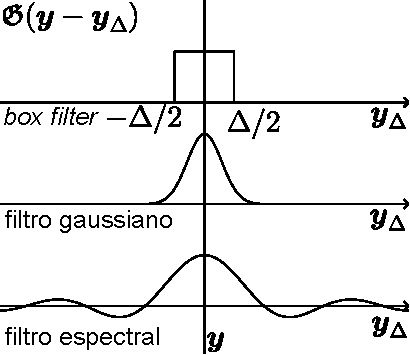
\includegraphics[width=\linewidth]{Figuras/filtros1.pdf}
        \caption{Função filtro.}
    \end{subfigure}
    \begin{subfigure}{0.4\textwidth}
        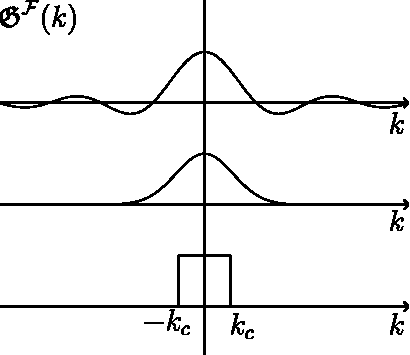
\includegraphics[width=\linewidth]{Figuras/filtros2.pdf}
        \caption{Transformada de Fourier.}
    \end{subfigure}
    \\Fonte: Autoria Própria (\the\year).
    \label{fig:Filters}
\end{figure}

O valor $\gamma_g$ observado no filtro gaussiano é uma constante, comumente atribuída com o valor de 6,0. Já o parâmetro $k_c$ é o número de onda de corte, dado por $k_c=\pi/\Delta$. Dentre os filtros apresentados, percebe-se que tanto o \textit{box filter} quanto o filtro gaussiano possuem suporte compacto no espaço físico, porém não possuem suporte compacto no espaço de Fourier, o que pode gerar problemas numéricos. Já o filtro espectral possui suporte compacto no espaço de Fourier, porém não possui suporte compacto no espaço físico.

Dessa maneira, é possível separar os efeitos das grandes escalas e das pequenas escalas, o que é ilustrado na Figura \ref{fig:EfeitoFiltragem} para uma distribuição de velocidade $\BB{u}$.

\begin{figure}[h!]
    \centering
    \caption{Efeito da filtragem sobre um campo de velocidades $\BB{u}$.}
    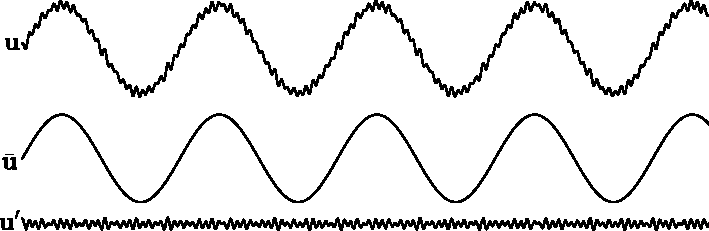
\includegraphics[width=.75\linewidth]{Figuras/efeito_filtragem.pdf}
    \\Fonte: \citeonline{hughes2000large} - Adaptado.
    \label{fig:EfeitoFiltragem}
\end{figure}

Assim, em uma descrição Euleriana, pode-se obter as equações de Navier-Stokes filtradas:

\begin{subequations}
    \begin{align}
         & \rho\bigpar{\dot{\BBB{u}}+\Ny\cdot(\overline{\BB{u}\otimes\BB{u}})-\BBB{f}}-\Ny\cdot\bar{\tens}=\BB{0} &  & \text{ em }\Omega\text{,} \\
         & \Ny\cdot\BBB{u}=0                                                                                      &  & \text{ em }\Omega\text{.}
    \end{align}
\end{subequations}

Pode-se perceber que o termo convectivo impede a completa separação dos termos $\BBB{u}$ e $\BB{u}'$ devido à sua natureza altamente não-linear. Por conta disso a parcela não filtrada não pode ser ignorada nesse problema, sendo necessário realizar algumas manipulações algébricas. Sabendo-se que $\BB{u}=\BBB{u}+\BB{u}'$, pode-se reescrever a equação da conservação da quantidade de movimento como:

\begin{equation}
    \rho\bigpar{\dot{\BBB{u}}+\Ny\cdot(\overline{(\BBB{u}+\BB{u}')\otimes(\BBB{u}+\BB{u}')})-\BBB{f}}-\Ny\cdot\bar{\tens}=\BB{0}
\end{equation}

Nesse sentido, surgirão termos cruzados entre $\BBB{u}$ e $\BB{u}'$, os quais serão condensados em um tensor de subescala (\textit{Subgrid-Scale} - SGS) $\BB{T}$ dado por \cite{piomelli1999large,hughes2000large}:

\begin{equation}
    \BB{T}=\BBB{u}\otimes\BBB{u}-\overline{\BB{u}\otimes\BB{u}}=-\bigpar{\BB{L}+\BB{C}+\BB{R}}\text{,}
\end{equation}

\noindent no qual $\BB{L}=\overline{\BBB{u}\otimes\BBB{u}}-\BBB{u}\otimes\BBB{u}$ é o tensor de Leonard, que representa as interações entre as grandes escalas, podendo ser determinado explicitamente e utilizado para análise de erros, $\BB{C}=\overline{\BBB{u}\otimes\BB{u}'}+\overline{\BB{u}'\otimes\BBB{u}}$ é o tensor de termos cruzados, representando a interação entre as grandes e pequenas escalas e $\BB{R}=\overline{\BB{u}'\otimes\BB{u}'}$ é o tensor de tensões SGS de Reynolds, que representa a interação entre as pequenas escalas \cite{piomelli1999large}. Assim pode-se escrever:

\begin{equation}
    \rho\bigpar{\dot{\BBB{u}}+\Ny\cdot(\BBB{u}\otimes\BBB{u})-\Ny\cdot\BB{T}-\BBB{f}}-\Ny\cdot\bar{\tens}=\BB{0}\text{.}
\end{equation}

Aplicando a incompressibilidade e substituindo-se $\bar{\tens}$ pelo modelo constitutivo \eqref{eq:ModConst}, tem-se que:

\begin{equation}
    \rho\bigpar{\dot{\BBB{u}}+(\BBB{u}\cdot\Ny)\BBB{u}-\Ny\cdot\BB{T}-\BBB{f}}-\mu\Ny\cdot(\Ny\BBB{u}+\NyT\BBB{u})+\Ny p=\BB{0}\text{,}\label{eq:ConMasLES}
\end{equation}

\noindent ou, dividindo-se por $\rho$ e fazendo algumas manipulações tem-se que:

\begin{equation}
    \dot{\BBB{u}}+(\BBB{u}\cdot\Ny)\BBB{u}+\frac{\Ny p}{\rho}=\nu\Lapl\BBB{u}+\Ny\BB{T}+\BBB{f}\text{,}
\end{equation}

\noindent sendo $\Lapl(\cdot)=\Ny\cdot\Ny(\cdot)$ o operador laplaciano e $\nu=\mu/\rho$ a viscosidade cinemática.

Assim, o problema fica governado por:

\begin{equation}
    \left\{
    \begin{array}{ll}
        \dot{\BBB{u}}+(\BBB{u}\cdot\Ny)\BBB{u}+\frac{\Ny p}{\rho}=\nu\Lapl\BBB{u}+\Ny\cdot\BB{T}+\BBB{f} & \text{ em }\Omega\text{,} \\
        \Ny\cdot\BBB{u}=0                                                                                & \text{ em }\Omega\text{,}
    \end{array}
    \right.
\end{equation}

\noindent havendo ainda a necessidade de se determinar um tensor $\BB{T}$, em especial o seu tensor desviador:

\begin{equation}
    \dev{\BB{T}}=\BB{T}-\frac{1}{3}\tr{(\BB{T})}\BB{I}\text{,}
\end{equation}

\noindent que descreva adequadamente as interações entre diferentes escalas. Isso pode se tornar problemático uma vez que não se possui solução para as pequenas escalas. Uma forma de se fazer isso é através do modelo de viscosidade de vórtice de Smagorinsky \cite{smagorinsky1963general}, resultando no tensor:

\begin{equation}
    \bigpar{\BB{T}_S}=2\nu_T\deffil\text{,}
\end{equation}

\noindent sendo $\nu_T$ a viscosidade de vórtice SGS, dada por \cite{germano1991dynamic,piomelli1999large,hughes2000large,bailly2015turbulence,katopodes2019free}:

\begin{equation}
    \nu_T=(C_S\Delta)^2\norm{\deffil}\text{,}
\end{equation}

\noindent onde $C_S$ é a constante de Smagorinsky e $\norm{\deffil}$ é a magnitude do tensor taxa de deformação em escala grosseira, dada por:

\begin{equation}
    \norm{\deffil}=(2\deffil:\deffil)^{1/2}\text{.}
\end{equation}

Note que o tensor $\BB{T}_S$ é um tensor desviador, ou seja, $\BB{T}_S=\dev{\BB{T}_S}$.

%\citeonline{germano1991dynamic,hughes2000large} ainda fazem algumas constatações sobre o modelo de Smagorinsky, os quais destacam-se o fato de $\BB{T}_S$ não possuir um comportamento assintótico próximo às paredes, o que se esperaria de $\BB{T}$, os valores de $C_S$ na presença de cisalhamento médio causaram amortecimentos excessivos e o tensor $\BB{T}_S$ impede a energia de fluir entre diferentes escalas, podendo ser significante em alguns casos.
%
%Como tentativa de se resolver esses problemas, \citeonline{germano1991dynamic} propuseram assumir $C_S$ como uma função $C_S=C_S(\BB{y},t)$, permitindo, assim, que esse parâmetro se adapte para melhor modelar as pequenas escalas.

Para a determinação da constante de Smagorinsky, realiza-se inicialmente uma aproximação da amplitude espectral da energia cinética $E(k)$, dada sobre a superfície de uma esfera parametrizada de raio $k$, de acordo com \cite{hughes2000large}:

\begin{equation}
    E(k)\approx\alpha\varepsilon^{2/3}k^{-5/3}\text{,}\label{eq:Ek1}
\end{equation}

\noindent em que $\alpha$ é a constante de Kolmogoroff e $\varepsilon$ é a dissipação turbulenta. A Figura \ref{fig:EnergiaEspectral} apresenta graficamente o comportamento da energia espectral em função de $k$.

\begin{figure}[h!]
    \centering
    \caption{Amplitude da energia espectral.}
    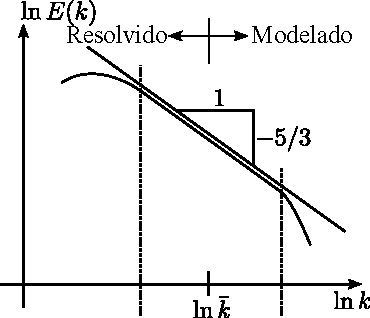
\includegraphics[width=0.4\linewidth]{Figuras/EnergiaEspectral.pdf}
    \\Fonte: \cite{hughes2000large} - Adaptado.
    \label{fig:EnergiaEspectral}
\end{figure}

O valor de $\norm{\deffil}$ é adotado como:

\begin{equation}
    \frac{1}{2}\norm{\deffil}=\int_0^{k_c}{k^2E(k)dk}\text{,}\label{eq:ndeffil1}
\end{equation}

\noindent sendo $k_c$ o limite de resolução.

Substituindo \eqref{eq:Ek1} em \eqref{eq:ndeffil1}, resolvendo a integral e fazendo algumas manipulações algébricas, tem-se que:

\begin{equation}
    \norm{\deffil}^3=\bigpar{\frac{3\alpha}{2}}^{3/2}k_c^2\varepsilon\text{.}
\end{equation}

Com isso, considerando também que a dissipação de energia cinética é igual àquela produzida, realiza-se o balanço da energia, obtendo-se:

\begin{equation}
    \varepsilon=\BB{T}_S:\deffil\text{.}
\end{equation}

\noindent Assim, fica possível obter expressões que relacionam os valores de $C_S$ $\Delta$ e $\nu_T$ com $k_c$:

\begin{equation}
    C_S\Delta=\bigpar{\frac{2}{3\alpha}}^{3/4}k_c^{-1}\text{ e}
\end{equation}

\begin{equation}
    \nu_T=\bigpar{\frac{2}{3\alpha}}\varepsilon^{1/3}k_c^{-4/3}\text{.}
\end{equation}

Segundo \citeonline{bailly2015turbulence} o valor de $k_c$ pode ser estimado como $k_c=\pi/\Delta$, o que leva à seguinte expressão para a constante de Smagorinsky:

\begin{equation}
    C_S=\frac{1}{\pi}\bigpar{\frac{2}{3\alpha}}^{3/4}\text{.}
\end{equation}

Com isso, um possível valor para a constante Kolmogoroff é $\alpha=1,4$, o que resulta em $C_S\approx0,18$. No entanto, segundo  \citeonline{hughes2000large,bailly2015turbulence,katopodes2019free}, valores de $C_S$ próximos à 0,10 conduzem a solução à resultados mais realistas.

\begin{comment}
%==================================================================================================
\subsubsection{Procedimento computacional} \label{LES-PC}
%==================================================================================================

Para a obtenção dos resultados, parte-se para a formulação variacional, em que se utiliza funções testes $\BB{w}$ e $q$, associadas às equações de conservação da quantidade de movimento e da continuidade, respectivamente. Assim, a forma fraca do problema LES é dada por:

\begin{equation}
    \begin{split}
        &\intDom{w_i\rho\bigpar{\dot{\ub}_i+\uub{j}\ub_{i,j}-\bar{f}_i}}+\intDom{\rho w_{i,j}T_{ij}}+\intDom{w_{i,j}\sigma_{ji}(\BB{\ub},\pb)}+\\
        &\intDom{q\ub_{i,i}}-\intNeumann{\rho w_iT_{ij}n_j}-\intNeumann{w_i\bar{h}_i}=0\text{.}
    \end{split}
\end{equation}

Substituindo o modelo constitutivo e o modelo de viscosidade de Smagorinsky tem-se que:

\begin{equation}
    \begin{split}
        &\intDom{w_i\rho\bigpar{\dot{\ub}_i+\uub{j}\ub_{i,j}-\bar{f}_i}}+\intDom{w_{i,j}(\mu+\rho\nu_T)(\uSim{\ub}{i}{j})}-\\
        &\intDom{w_{i,i}\pb}+\intDom{q\ub_{i,i}}-\intNeumann{w_i\bar{h}_i}=0\text{.}
    \end{split}
\end{equation}

\textcolor{purple}{
    No intuito de se obter uma solução estável, será considerado o elemento de Taylor-Hood P2P1 (aproximação quadrática para o campo de velocidades e linear para o campo de pressões) na formulação. Assim denomina-se $M$ as funções de forma para aproximação quadrática e $N$ para funções de forma lineares. Com isso, faz-se a aproximação das funções testes por meio das funções de forma, tendo como resultado os seguintes vetores de resíduo associados às equações de conservação de momento e da continuidade:
}
\textcolor{red}{1. Você deve deixar a formulação geral, e nos exemplos dizer o que você utilizou para obter resposta estável. Sugiro que desde o início (VMS) você diferencie as funções de forma de pressão e de velocidade (eu prefiro colocar um sobrescrito u e p ao invés de usar N e M). Aqui você deveria apresentar a formulação estabilizada, e nos exemplos você diz o que adotou para rodar. De qualquer forma, aqui ficou faltando colocar a estabilização para a convecção (SUPG) que sempre será necessária. Reveja o restante deste item com base nisso...}

\begin{subequations}
    \begin{equation}
        \begin{split}
            \bigpar{N_M}_i^a=&\intDom{M_a\rho\bigpar{\dot{\ub}_i+\uub{j}\ub_{i,j}-\bar{f}_i}}+\\
            &\intDom{M_{a,j}(\mu+\rho\nu_T)(\uSim{\ub}{i}{j})}-\intDom{M_{a,i}\pb}-\intNeumann{N_a\bar{h}_i}\text{ e}
        \end{split}
    \end{equation}
    \begin{equation}
        \bigpar{N_C}^a=\intDom{N_a\ub_{i,i}}\text{.}
    \end{equation}
    \label{eq:VetoresResiduo-LES}
\end{subequations}

Dessa forma procura-se determinar valores de $\ub$ e $\pb$ que anulem $N_M$ e $N_C$. Para esse fim utiliza-se o método de Newton-Raphson, em que as variáveis a serem determinadas são as acelerações e pressões nodais, sendo o integrador utilizado o $\alpha$-generalizado, apresentado na seção \ref{IT-VMS}. Desse modo tem-se os seguintes sub-blocos que compõem a matriz tangente:

\begin{subequations}
    \begin{equation}
        \begin{split}
            \der{(N_M)_i^a}{\dot{U}_j^b}=&\alpha_m\intDom{\rho M_aM_b}\dij+\beta_f\intDom{\rho M_aM_b\ub_{i,j}}+\\
            &\beta_f\intDom{\rho M_aM_{b,k}\uub{k}}\dij+\beta_f\intDom{(\mu+\rho\nu_T)M_{a,k}M_{d,k}}\dij+\\
            &\beta_f\intDom{(\mu+\rho\nu_T)M_{a,j}M_{b,i}}\text{,}
        \end{split}
    \end{equation}
    \begin{equation}
        \der{(N_M)_i^a}{P^b}=-\intDom{M_{a,i}N_b}\text{,}
    \end{equation}
    \begin{equation}
        \der{(N_C)^a}{\dot{U}_j^b}=\beta_f\intDom{N_aM_{b,j}}\text{ e}
    \end{equation}
    \begin{equation}
        \der{(N_C)^a}{P^b}=0\text{.}
    \end{equation}
    \label{eq:MatrizTangente-LES}
\end{subequations}

\noindent em que $\beta_f=\alpha_f\gamma\Delta t$.

Observa-se que o sub-bloco $\partial{\NC}/\partial\BB{P}$ está presente na diagonal principal do problema, possuindo valor nulo. Isso pode ser interpretado como a consideração das pressões como multiplicadores de Lagrange nessa formulação.

%Para obtenção da solução aproximada, utiliza-se um procedimento similar ao apresentado no algoritmo \ref{alg:MEF-VMS}, onde o comando \ref{alg:estabilizador} é alterado para computar o valor da viscosidade de vórtice, assim como os valores das componentes da matriz tangente e dos vetores de resíduo são alterados para se adequarem ao presente modelo.
\end{comment}
%==================================================================================================
\subsection{\textit{Reynolds-Averaged Navier-Stokes}} \label{RANS}
%==================================================================================================

A aproximação das equações diferenciais denominada \textit{Reynolds-Averaged Navier-Stokes} (RANS) busca encontrar uma solução a partir da chamada decomposição de Reynolds. Nesse contexto, observa-se que simulações feitas utilizando RANS são mais eficientes computacionalmente que aquelas feitas a partir de LES, além de possuírem uma implementação mais simples \cite{alfonsi2009reynolds, ling2015evaluation}.

Considera-se que uma propriedade $\phi$ pode ser decomposta em duas parcelas: uma referente à média, denotada por uma barra ($\bar{\phi}(\BB{y},t)$), e uma referente à flutuações no espaço-tempo, denotada por $\phi'(\BB{y},t)$, ou seja, $\phi(\BB{y},t)=\bar{\phi}+\phi'$.

No entanto, há diferentes formas de se considerar a média de uma propriedade, tal como: média temporal, comumente utilizada em escoamentos estacionários; média espacial, utilizada em escoamentos turbulentos homogêneos; e média de um conjunto de experimentos \cite{tennekes1972first,speziale1991analytical,alfonsi2009reynolds}. Como apontado por \citeonline{speziale1991analytical,alfonsi2009reynolds}, a última opção é adequada para descrever escoamentos que não são nem estacionários, nem homogêneos, sendo calculada como:

\begin{equation}
    \bar{\phi}(\BB{y},t)=\lim_{n\to\infty}{\frac{1}{n}\sum_{k=1}^n{\phi^{k}(\BB{y},t)}}\text{,}
\end{equation}

\noindent em que $n$ é o número de experimentos realizados.

Vale ressaltar algumas propriedades interessantes relacionadas à média de uma propriedade ($\phi$, $\phi_1$ ou $\phi_2$ quaisquer), tais como:

\begin{enumerate}[label=\alph*.]
    \item $\bar{\phi}'=0$;
    \item $\bar{\bar{\phi}}=\bar{\phi}$;
    \item $\bar{\phi_1+\phi_2}=\bar{\phi}_1+\bar{\phi}_2$;
    \item $\bar{\phi_1\bar{\phi}_2}=\bar{\phi}_1\bar{\phi}_2$;
    \item $\bar{\phi_1\phi_2}=\bar{\phi}_1\bar{\phi}_2+\bar{\phi_1'\phi_2'}$;
    \item $\bar{\Ny\phi}=\Ny\bar{\phi}$; e
    \item $\bar{\dot{\phi}}=\dot{\bar{\phi}}$.
\end{enumerate}

Assim, pode-se tomar a média das Equações de Navier-Stokes, obtendo-se:

\begin{subequations}
    \begin{align}
         & \rho\bigpar{\bar{\dot{\BB{u}}}+\bar{\Ny\cdot(\BB{u}\otimes\BB{u})}-\BBB{f}}-\bar{\Ny\cdot\tens}=\BB{0} &  & \text{ em }\Omega\text{,} \\
         & \bar{\Ny\cdot\BB{u}}=0                                                                                 &  & \text{ em }\Omega\text{.}
    \end{align}
\end{subequations}

Aplicando também o modelo constitutivo apresentado em \ref{MC}, o problema se torna:

\begin{subequations}
    \begin{align}
         & \rho\bigpar{\dot{\BBB{u}}+\Ny\cdot(\bar{\BB{u}\otimes\BB{u}})-\BBB{f}}-\mu\Lapl\BBB{u}+\Ny\bar{p}=\BB{0} &  & \text{ em }\Omega\text{,} \\
         & \Ny\cdot\BBB{u}=0                                                                                        &  & \text{ em }\Omega\text{.}
    \end{align}
\end{subequations}

Realizando a separação das variáveis em suas respectivas parcelas na equação da conservação de movimento, tem-se que:

\begin{equation}
    \rho\bigpar{\dot{\BBB{u}}+\Ny\cdot\bar{(\BBB{u}+\BB{u}')\otimes(\BBB{u}+\BB{u}')}-\BBB{f}}-\mu\Lapl{\BBB{u}}+\Ny\bar{p}=\BB{0}\text{,}
\end{equation}

\noindent que leva à seguinte expressão simplificada:

\begin{equation}
    \rho\bigpar{\dot{\BBB{u}}+\BBB{u}\cdot\Ny\BBB{u}+\Ny\cdot(\bar{\BB{u}'\otimes\BB{u}'})-\BBB{f}}-\mu\Lapl\BBB{u}+\Ny\bar{p}=\BB{0}\text{,}
    \label{eq:RANS-estac}
\end{equation}

\noindent a qual representa a equação RANS da quantidade de movimento para escoamentos incompressíveis \cite{chou1945velocity,alfonsi2009reynolds}.

Nesse contexto vale mencionar o tensor de tensões de Reynolds (dividido pela densidade), dado por $\btau=-\bar{\BB{u}'\otimes\BB{u}'}$, traz a interferência que os efeitos turbulentos que a parcela de flutuação causa no movimento médio \cite{chou1945velocity,alfonsi2009reynolds}. Porém, verifica-se que, ao assumir essa separação de variáveis, o problema conta com mais incógnitas do que equações para as determinar. Logo, uma forma de se obter equações adicionais que auxiliem na resolução do problema se encontra na modelagem do tensor de tensões de Reynolds de forma a relacionar as flutuações de velocidades com as velocidades médias.

\citeonline{alfonsi2009reynolds} aponta que problemas envolvendo RANS podem ser classificados dependendo da quantidade de equações diferenciais resolvidas, em que cada equação adicionada se refere ao transporte de uma propriedade relativa à turbulência, alterando, assim, a maneira com que a viscosidade de vórtice é determinada. Segundo o autor, as classes de modelos RANS de turbulência são:

\begin{enumerate}[label=\alph*.]
    \item Modelos de Zero Equações: Apenas as equações referentes ao campo médio são resolvidas, sendo $l_0$ e $\tau_0$ determinados empiricamente;
    \item Modelos de Uma Equação: É adicionada uma equação de transporte em termos da energia cinética média $k$ para auxiliar na determinação do campo de flutuações de velocidades;
    \item Modelos de Duas Equações: Uma segunda equação é adicionada para determinação das escalas de comprimento turbulento;
    \item Modelos de Tensões: A respeito aos Modelos de Zero Equações, adiciona-se duas equações de transporte referentes ao tensor de Reynolds e à $\varepsilon$, tal modelo também pode ser chamado de modelo $\te$.
\end{enumerate}

Sobre os Modelos de Duas Equações, destacam-se os modelos $\ke$ \cite{haakansson2012experimental,davidson2014pans,parente2011improved}, nos quais as equações adicionais são dadas em função da energia cinética média gerada pelo campo de flutuações ($k$) e da taxa de dissipação da energia cinética turbulenta ($\varepsilon$) e $\kw$ \cite{larsen2018over,bassi2005discontinuous}, que ao invés de adicionar uma equação em termos de $\varepsilon$, esta de dá em função da escala de tempo turbulento recíproco ($\omega=\varepsilon/K$).

Dentre os modelos $\ke$, $\kw$ e $\te$, observa-se que o primeiro possui menor custo computacional e maior facilidade de implementação, sendo uma boa alternativa para as simulações \cite{koutsourakis2012evaluation,adanta2020comparison}.

Para se obter as equações adicionais, faz-se a simples substituição de $\BB{u}=\umed+\BB{u}'$ e $p=\bar{p}+p'$ na equação da quantidade de movimento, o que leva a:

\begin{equation}
    \begin{split}
        &\rho\bigpar{\dot{\BBB{u}}+\dot{\BB{u}'}+\BBB{u}\cdot\Ny\BBB{u}+\BBB{u}\cdot\Ny\BB{u}'+\BB{u}'\cdot\Ny\BBB{u}+\BB{u}'\cdot\Ny\BB{u}'-\BBB{f}}-\mu\Lapl\BBB{u}-\\
        &\mu\Lapl\BB{u}'+\Ny\bar{p}+\Ny p'=\BB{0}\text{.}
    \end{split}
    \label{eq:NS-RANS1}
\end{equation}

Subtraindo \eqref{eq:RANS-estac} de \eqref{eq:NS-RANS1} obtém-se:

\begin{equation}
    \rho\bigpar{\dot{\BB{u}'}+\BBB{u}\cdot\Ny\BB{u}'+\BB{u}'\cdot\Ny\BBB{u}+\BB{u}'\cdot\Ny\BB{u}'-\Ny\cdot\btau}-\mu\Lapl\BB{u}'+\Ny p'=\BB{0}\text{.}
    \label{eq:NS-RANS2}
\end{equation}

Seguindo o mesmo procedimento para a equação da conservação da massa obtém-se que:

\begin{equation}
    \Ny\cdot\BB{u}'=0\text{,}
\end{equation}

\noindent sendo equivalente à condição de incompressibilidade no campo de flutuações de velocidade.

Fazendo a contração em \eqref{eq:NS-RANS2} por meio de $\BB{u}'$, tomando a média, dividindo por $\rho$ e realizando as devidas simplificações tem-se a equação que descreve de forma exata o comportamento da energia cinética média gerada pelo campo de flutuações ($K=\bar{\norm{\BB{u}'}^2}/2$) \cite{alfonsi2009reynolds}:

%\begin{equation}
%    \bar{\BB{u}'\cdot\dvt{\BB{u}'}}+\bar{\BB{u}'\cdot(\BBB{u}\cdot\Ny\BB{u}')}+\bar{\BB{u}'\cdot(\BB{u}'\cdot\Ny\BBB{u})}+\bar{\BB{u}'\cdot(\BB{u}'\cdot\Ny\BB{u}')}+\bar{\BB{u}'\cdot(\Ny\cdot\btau)}-\bar{\nu\BB{u}'_i\cdot\Lapl\BB{u}'}+\bar{\BB{u}'\cdot\Ny\pr'}=0\text{.}
%\end{equation}

\begin{equation}
    \dot{K}+\BBB{u}\cdot\Ny K=\btau:\Ny\BBB{u}-\frac{\nu}{2}\bar{\norm{\Ny\BB{u}'}^2}-\Ny\cdot\bigpar{\frac{\bar{\norm{\BB{u}'}^2\BB{u}'}}{2}+\bar{\pr'\BB{u}'}}+\nu\Lapl K\text{,}
    \label{eq:Ke-K}
\end{equation}

\noindent em que $\pr'=p'/\rho$. Assim, \eqref{eq:Ke-K} pode ainda ser reescrita de forma mais compacta, considerando-se o efeito de cada parcela:

\begin{equation}
    \dot{K}+\BBB{u}\cdot\Ny K=P_K-\varepsilon-\Ny\cdot\BB{D}+\nu\Lapl K\text{,}
\end{equation}

\noindent em que $P_K$ é a produção da energia cinética turbulenta, a qual não precisa de modelagem, $\varepsilon$ é a taxa de dissipação turbulenta da energia cinética, $D_j$ é o gradiente de difusão turbulenta e o último termo, que dispensa modelagem, representa a difusão viscosa. Tais termos são dados por:

\begin{subequations}
    \begin{align}
         & P_K=\btau:\Ny\BBB{u}\text{,}                                             \\
         & \varepsilon=\frac{\nu}{2}\bar{\norm{\Ny\BB{u}'}^2}\text{ e}              \\
         & \BB{D}=\frac{\bar{\norm{\BB{u}'}^2\BB{u}'}}{2}+\bar{\pr'\BB{u}'}\text{.}
    \end{align}
\end{subequations}

\citeonline{alfonsi2009reynolds} apresenta que uma forma de se modelar os termos $\varepsilon$ e $\BB{D}$ como:

\begin{subequations}
    \begin{equation}
        \varepsilon=C^*\frac{K^{3/2}}{l_0}\text{ e}\\
    \end{equation}
    \begin{equation}
        \BB{D}=-\frac{\nu_T}{\sigma_K}\Ny K\text{,}
    \end{equation}
\end{subequations}

\noindent sendo $l_0$ o comprimento de vórtice, $C^*=0,166$ e $\sigma_K=1,0$ constantes adimensionais.

Há ainda a necessidade de se modelar o tensor de Reynolds, o qual pode ser subdividido em duas parcelas: uma parte isotrópica ($\btau^\mathrm{I}$) e outra desviadora ($\btau^\mathrm{D}$), ou seja:

\begin{equation}
    \btau=\btau^\mathrm{I}+\btau^\mathrm{D}\text{,}
\end{equation}

\noindent em que:

\begin{subequations}
    \begin{align}
         & \btau^\mathrm{I}=-\frac{2}{3}K\BB{I}\text{ e} \\
         & \btau^\mathrm{D}=2\nu_T\epmean\text{,}
    \end{align}
\end{subequations}

\noindent $\epmean_{ij}$ é a taxa de deformação do campo de velocidades média:

\begin{equation}
    \epmean=\frac{1}{2}(\Ny\BBB{u}+\NyT\BBB{u})
\end{equation}

\noindent e $\nu_T$ é a viscosidade de vórtice, dada por

\begin{equation}
    \nu_T=C_\mu\frac{K^2}{\varepsilon}\text{,}
\end{equation}

\noindent sendo $C_\mu=0,09$.

Já a equação exata do transporte que descreve a taxa de dissipação turbulenta da energia cinética ($\ep$) também é proveniente da equação \eqref{eq:NS-RANS2}, onde toma-se o gradiente da equação, realiza-se a contração dupla por meio de $\nu\Ny\BB{u}'/\rho$ e toma-se a média de todos os termos. Assim, após as simplificações tem-se, em sua forma indicial:

\begin{equation}
    \begin{split}
        &\dot{\ep}+\bar{u}_k\ep_{,k}=-2\nu\bar{u'_{i,j}u'_{k,j}}\bar{u}_{i,k}-2\nu\bar{u'_{i,j}u'_{i,k}}\bar{u}_{k,j}-2\nu\bar{u'_{i,j}u'_k}\bar{u}_{i,jk}-\\
        &2\nu\bar{u'_{i,j}u'_{k,j}u'_{i,k}}-\nu\bigpar{\bar{u'_{i,j}u'_{i,j}u'_k}}_{,k}-2\nu(\bar{u'_{i,j}\pr'_{,j}})_{,i}-2\nu^2\bar{u'_{i,jk}u'_{i,jk}}+\nu\ep_{,kk}\text{,}
    \end{split}
\end{equation}

\noindent sendo a vírgula presente no subíndice referente à derivada na direção indicada.

Fazendo a simplificação em termos dos efeitos de cada parcela tem-se:

\begin{equation}
    \dot{\ep}+\uub{k}\ep_{,k}=P_\ep+D_\ep-\Phi_\ep+\nu\ep_{,kk}\text{,}
\end{equation}

\noindent em que $P_\ep$ é a produção de dissipação, $D_\ep$ é a difusão turbulenta de dissipação, $\Phi_\ep$ é a destruição turbulenta da dissipação e o último termo é o transporte viscoso. Essas parcelas são dadas de forma exata por:

\begin{subequations}
    \begin{align}
         & P_\ep=-2\nu\bar{u'_{i,j}u'_{k,j}}\bar{u}_{i,k}-2\nu\bar{u'_{i,j}u'_{i,k}}\bar{u}_{k,j}-2\nu\bar{u'_{i,j}u'_k}\bar{u}_{i,jk}-2\nu\bar{u'_{i,j}u'_{k,j}u'_{i,k}} \text{,} \\
         & D_\ep=-\nu\bigpar{\bar{u'_{i,j}u'_{i,j}u'_k}}_{,k}-2\nu(\bar{u'_{i,j}\pr'_{,j}})_{,i} \text{ e}                                                                         \\
         & \Phi_\ep=2\nu^2\bar{u'_{i,jk}u'_{i,jk}}\text{.}
    \end{align}
\end{subequations}

Assim, realiza-se uma modelagem sobre os termos necessários como:

\begin{subequations}
    \begin{align}
         & P_\ep=C_{\ep 1}\frac{\ep}{k}\btau:\Ny\BBB{u}\text{,}          \\
         & D_\ep=\Ny\cdot\bigpar{\frac{\nu_T}{\sigma_\ep}\Ny\ep}\text{e} \\
         & \Phi_\ep=C_{\ep 2}\frac{\ep^2}{K}\text{,}
    \end{align}
\end{subequations}

\noindent em que $C_{\ep 1}=1,44$, $C_{\ep 2}=1,92$ e $\sigma_\ep=1,3$ são constantes adimensionais.

Assim, o problema RANS fica descrito pelas equações:

\begin{equation}
    \left\{
    \begin{array}{l}
        \rho\bigpar{\dot{\BBB{u}}+\BBB{u}\cdot\Ny\BBB{u}-\Ny\cdot\btau-\BBB{f}}-\mu\Lapl\BBB{u}+\Ny\bar{p}=\BB{0} \\
        \Ny\cdot\BBB{u}=0                                                                                         \\
        \dot{K}+\BBB{u}\cdot\Ny K=P_K-\varepsilon-\Ny\cdot\BB{D}+\nu\Lapl K                                       \\
        \dot{\varepsilon}+\BBB\cdot\Ny\ep=P_\ep+D_\ep-\Phi_\ep+\nu\Lapl\ep                                        \\
        \btau=-\frac{2}{3}K\BB{I}+\nu_T(\Ny\BBB{u}+\NyT\BBB{u})                                                   \\
        \nu_T=C_\mu\frac{K^2}{\ep}\text{.}
    \end{array}
    \right.
\end{equation}
%%==================================================================================================
\subsection{Exemplos Numéricos} \label{ExemplosMT}
%==================================================================================================

Na presente seção serão apresentadas algumas simulações realizadas utilizando os modelos VMS e LES, com a finalidade de validar os modelos implementados.

%==================================================================================================
\subsubsection{Cavidade bidimensional}
%==================================================================================================

A primeira simulação é um problema comumente utilizado na literatura como \textit{benchmark}, o qual trata-se de uma cavidade quadrada ($\Omega=[-1,1]^2$) com paredes aderentes, onde o fluido encontra-se confinado e sujeito a uma velocidade prescrita $\BB{u}_\infty$ ocasionada devido ao deslizamento de uma parede na face superior da cavidade. Nesse sentido serão observados os efeitos provocados no fluido devido à diferentes números de Reynolds, o qual é calculado por meio da equação \ref{eq:Reynolds}:

\begin{equation}
    \Rey=\frac{\rho L\norm{\BB{u}_\infty}}{\mu}\text{,}
    \label{eq:Reynolds}
\end{equation}

\noindent em que $L$ é o comprimento característico, que no caso analisado é igual ao lado da cavidade. Dessa forma considera-se uma velocidade constante para todas as análises de $\BB{u}_\infty=\{1,0\}^T$, sendo os diferentes números de Reynolds obtidos pela variação da viscosidade do fluido. A Figura \ref{fig:cavity} apresenta esquematicamente o problema simulado.

\begin{figure}[h!]
    \centering
    \caption{Desenho esquemático do problema de cavidade.}
    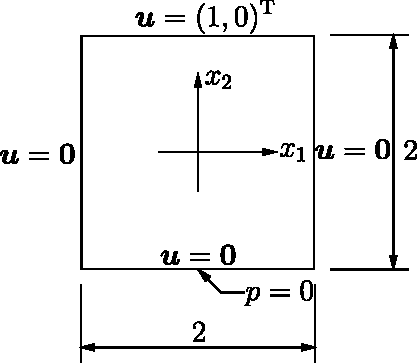
\includegraphics[width=.35\linewidth]{Figuras/Cavity/cavidade.pdf}
    \\Fonte: Autoria Própria (\the\year).
    \label{fig:cavity}
\end{figure}

Pelo fato do problema possuir apenas fronteiras do tipo Dirichlet, o condicionamento da solução do campo de pressões é garantido pela aplicação de uma condição de pressão nula no vértice superior direito da cavidade, conforme visto na figura acima.  Também se observa que existe uma descontinuidade nas condições de contorno no encontro entre as paredes da cavidade e seu topo, podendo ser consideradas velocidades nulas ou igual à velocidade do topo. No problema em questão considerou-se que a velocidade nesse ponto é igual à $\BB{u}_\infty$.

A malha de elementos finitos foi feita pela subdivisão do domínio em 20000 elementos dispostos de maneira estruturada com orientação à esquerda, conforme observado na Figura \ref{fig:cavity_disc}. O número de graus de liberdade para a simulação VMS de aproximação linear, quadrática e LES são 30603, 121203 e 91003, respectivamente. Os parâmetros utilizados foram $\rho=1$ para todas as análises, $\mu=0,02$, $\mu=5\times10^{-3}$, $\mu=2\times10^{-3}$, $\mu=4\times10^{-4}$, $\mu=2,6667\times10^{-4}$ e $\mu=2\times10^{-4}$, resultando em $\Rey=100$, $\Rey=400$, $\Rey=1000$, $\Rey=5000$, $\Rey=7500$ e $\Rey=10000$, respectivamente. Os modelos utilizados foram o VMS com aproximação linear e quadrática e o LES com elementos de Taylor-Hood P2P1 e $C_S=0,10$. O passo de tempo em todos os casos foi de $\Delta t=0,1$ e a simulação foi mantida até que a estacionariedade dos parâmetros do fluxo fosse alcançada.

\begin{figure}[h!]
    \centering
    \caption{Malha considerada para o problema de cavidade.}
    
\includegraphics[width=.6\linewidth]{Figuras/Cavity/mesh.pdf}
    \\Fonte: Autoria Própria (\the\year).
    \label{fig:cavity_disc}
\end{figure}

Como o problema apresenta características de um escoamento quase-estático, a parcela dos termos inerciais foram desprezados em ambos os modelos de turbulência. Além disso, os resultados adquiridos para um determinado número de Reynolds foram aplicados como valores iniciais para a determinação dos resultados para a próxima análise.

Os resultados obtidos foram comparados com aqueles apresentados por \citeonline{ghia1982high}. A Figura \ref{fig:cavity-results} apresenta os valores do campo de velocidades sobre as linhas médias da cavidade ($x_1=0$ e $x_2=0$).

\begin{figure}[h!]
    \centering
    \caption{Valores do campo de velocidades sobre as linhas médias da cavidade.}
    \begin{subfigure}{0.4\textwidth}
        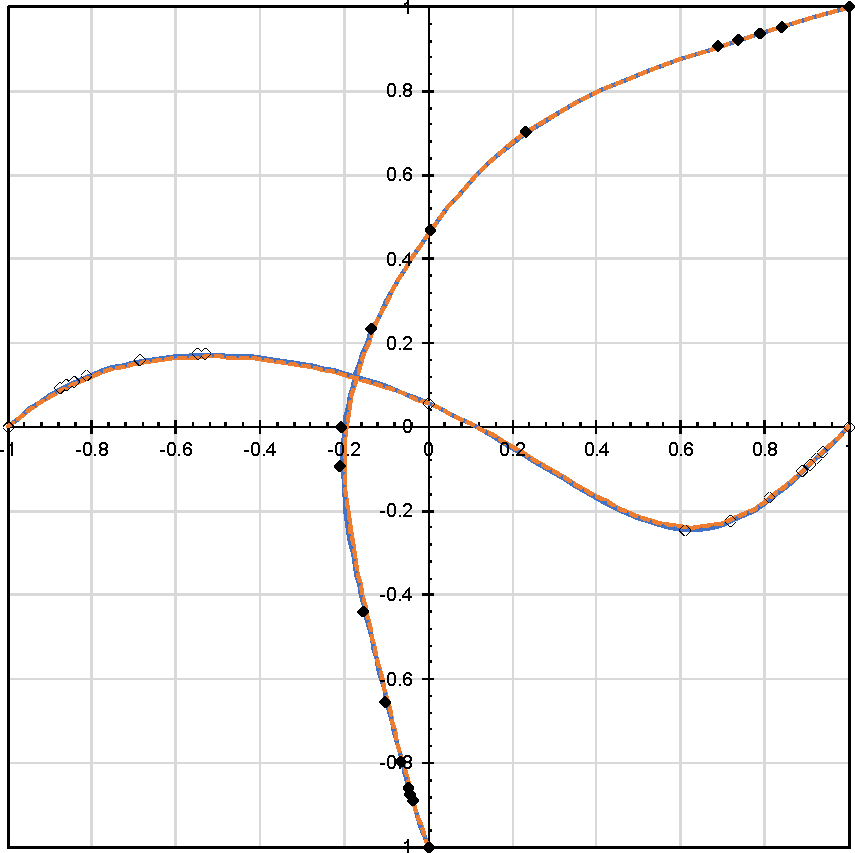
\includegraphics[width=\linewidth]{Figuras/Cavity/Re100.pdf}
        \caption{$\Rey=100$}
    \end{subfigure}
    \begin{subfigure}{0.4\textwidth}
        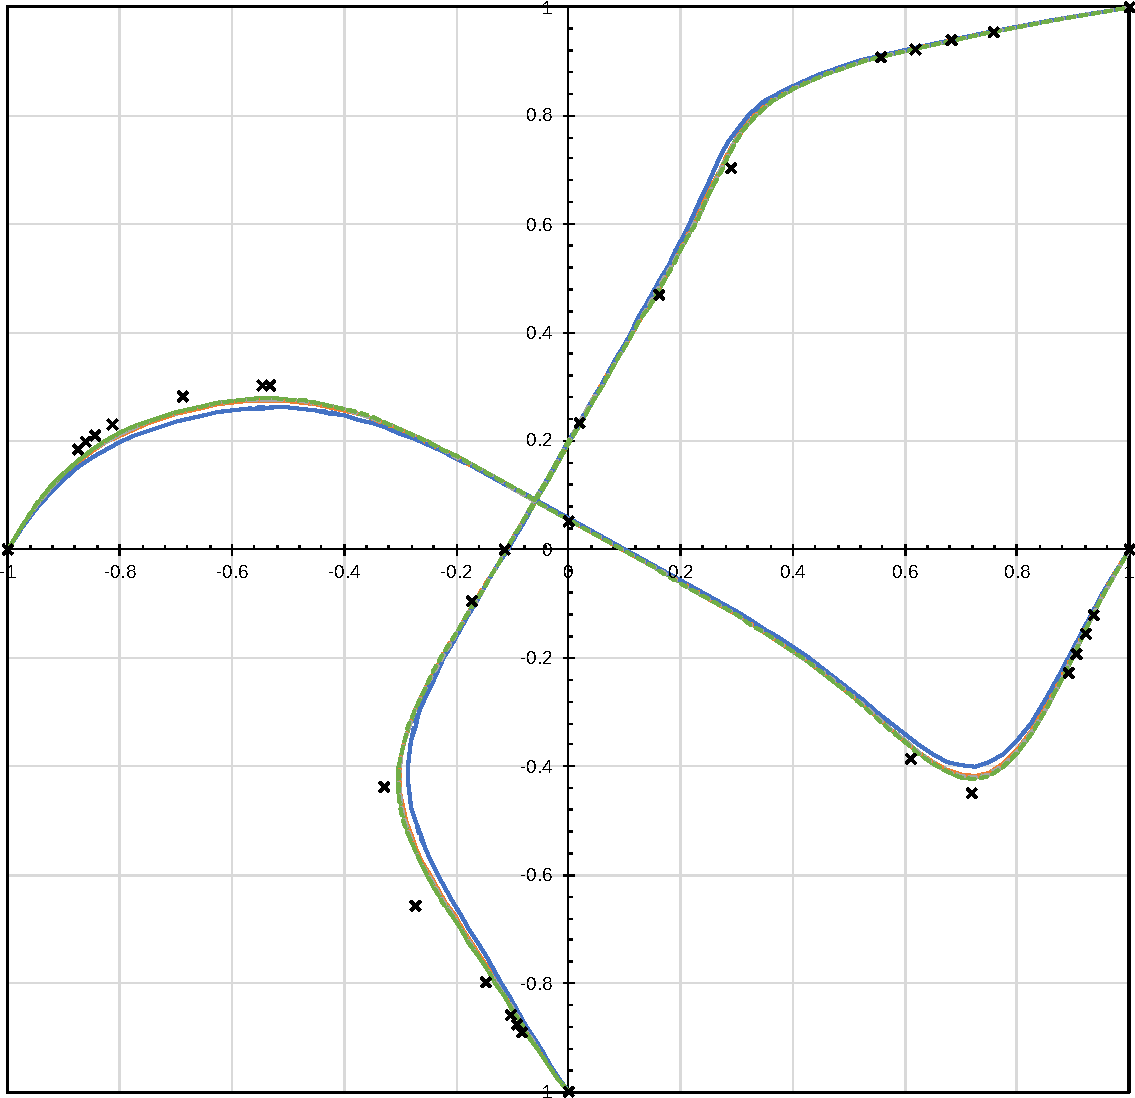
\includegraphics[width=\linewidth]{Figuras/Cavity/Re400.pdf}
        \caption{$\Rey=400$}
    \end{subfigure}
    \begin{subfigure}{0.4\textwidth}
        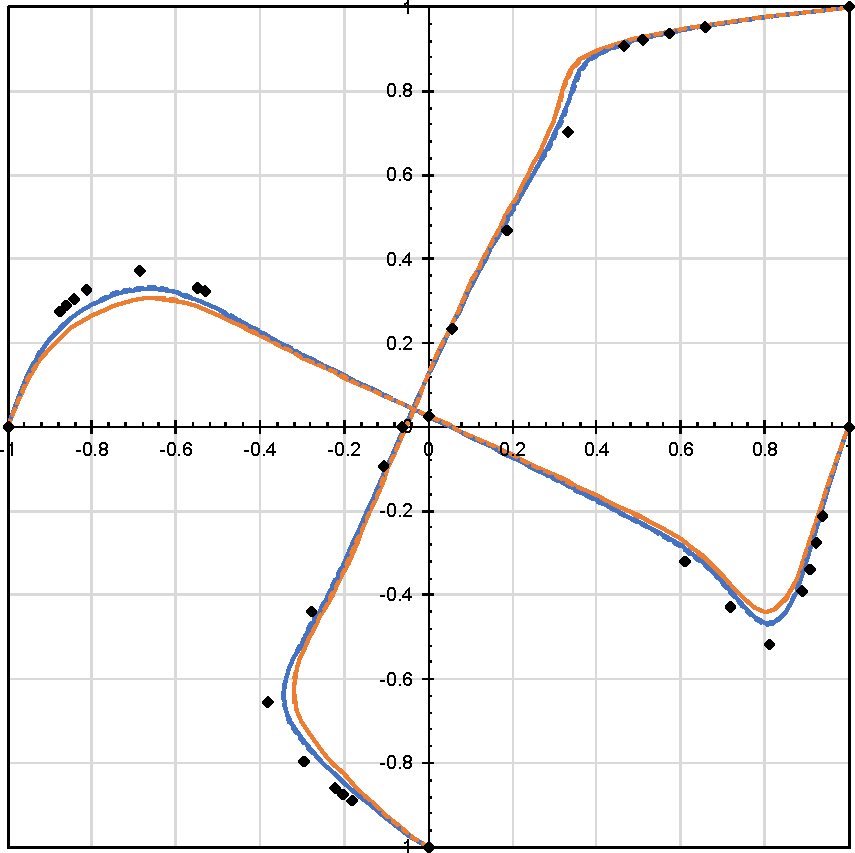
\includegraphics[width=\linewidth]{Figuras/Cavity/Re1000.pdf}
        \caption{$\Rey=1000$}
    \end{subfigure}
    \begin{subfigure}{0.4\textwidth}
        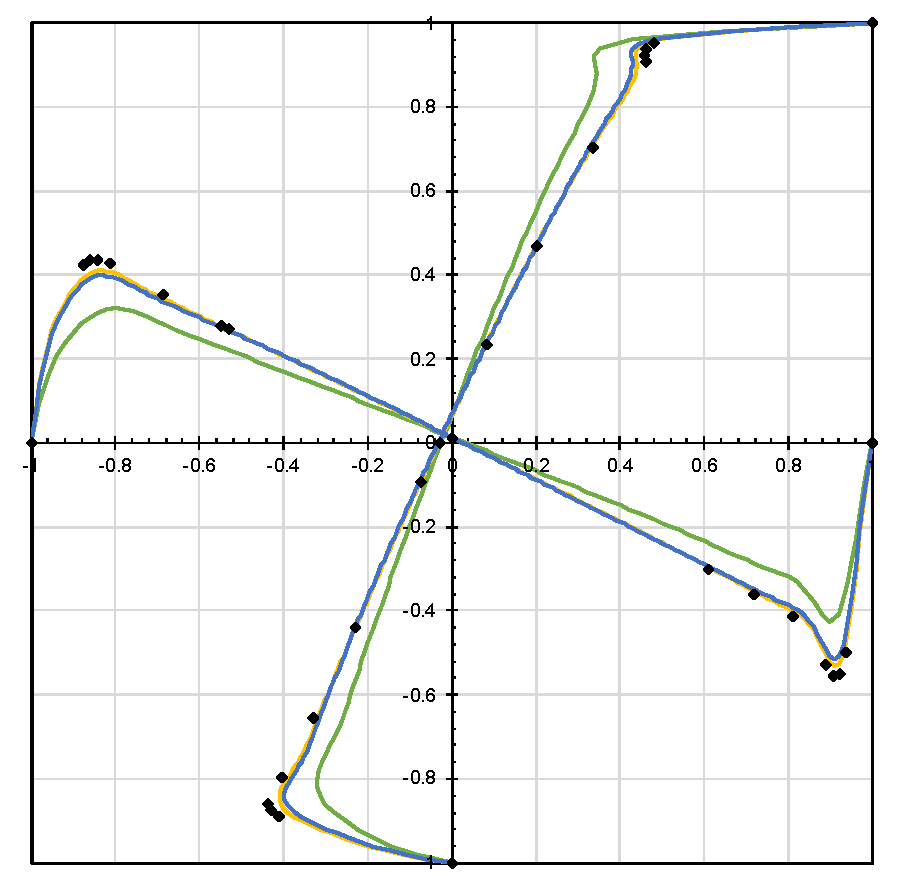
\includegraphics[width=\linewidth]{Figuras/Cavity/Re5000.pdf}
        \caption{$\Rey=5000$}
    \end{subfigure}
    \begin{subfigure}{0.4\textwidth}
        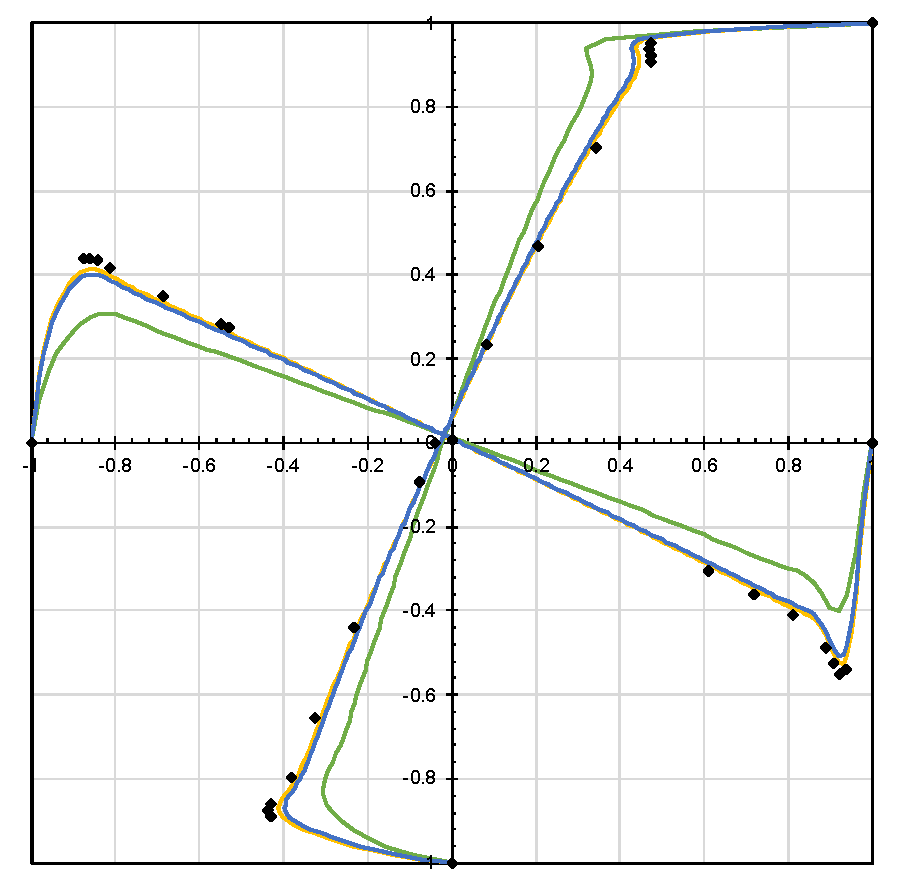
\includegraphics[width=\linewidth]{Figuras/Cavity/Re7500.pdf}
        \caption{$\Rey=7500$}
    \end{subfigure}
    \begin{subfigure}{0.4\textwidth}
        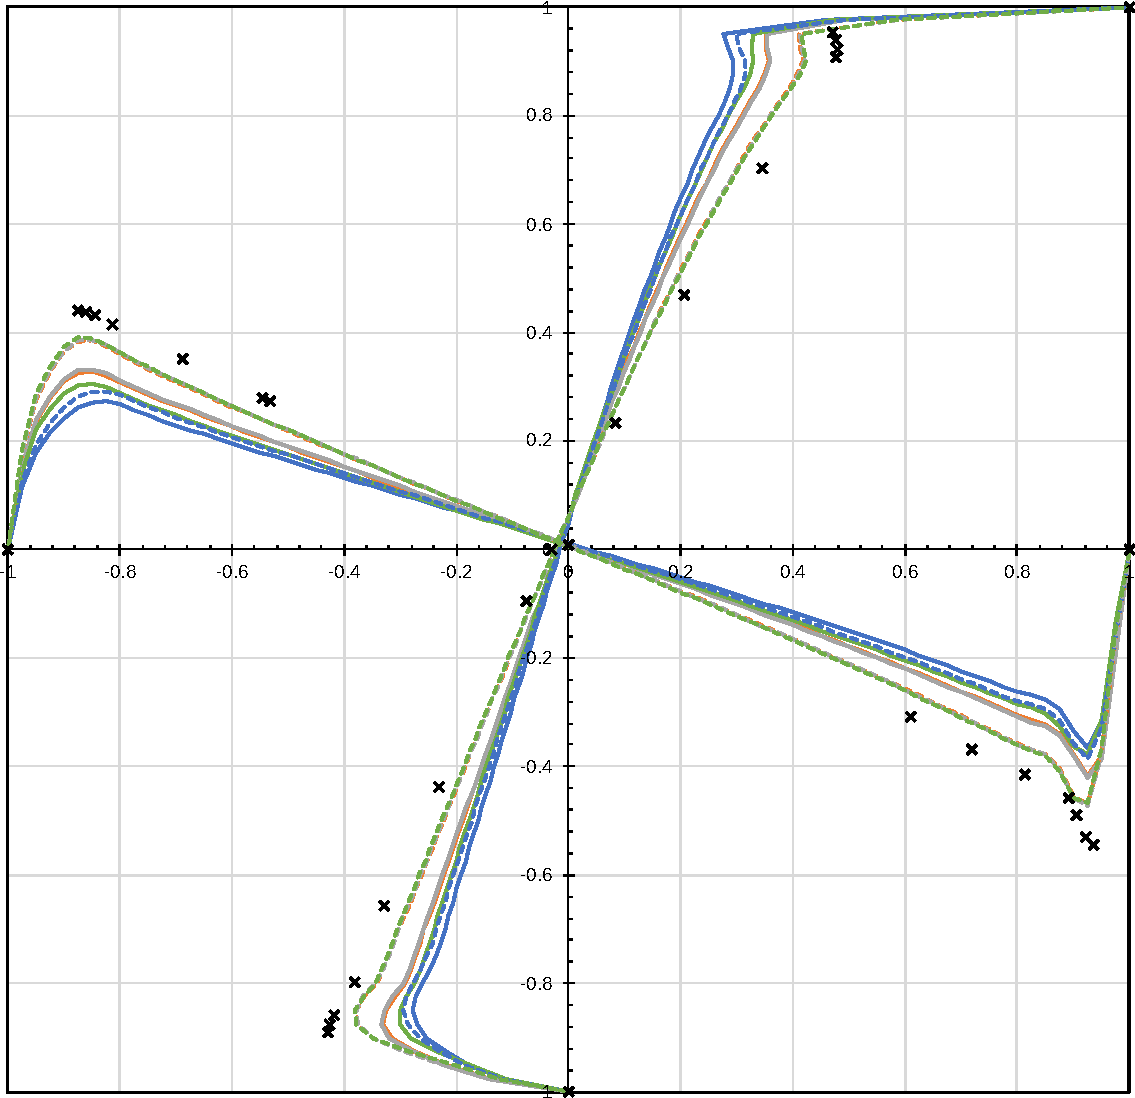
\includegraphics[width=\linewidth]{Figuras/Cavity/Re10000.pdf}
        \caption{$\Rey=10000$}
    \end{subfigure}
    \begin{subfigure}{\textwidth}
        
\includegraphics[width=\linewidth]{Figuras/Cavity/Legenda.pdf}
    \end{subfigure}
    \\Fonte: Autoria Própria (\the\year).
    \label{fig:cavity-results}
\end{figure}

A Figura \ref{fig:cavity-results2} apresenta o campo de velocidades na cavidade após o escoamento atingir seu estado estacionário.

\begin{figure}[h!]
    \centering
    \caption{Campo de velocidades em regime estacionário na cavidade.}
    \begin{subfigure}{0.32\textwidth}
        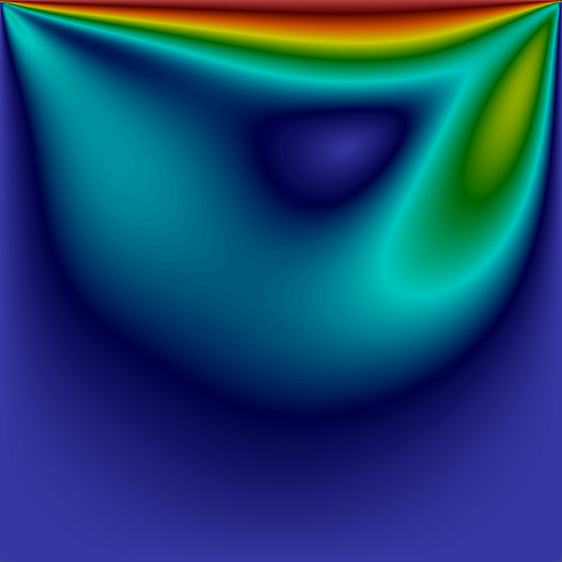
\includegraphics[width=\linewidth]{Figuras/Cavity/Re100.png}
        \caption{$\Rey=100$}
    \end{subfigure}
    \begin{subfigure}{0.32\textwidth}
        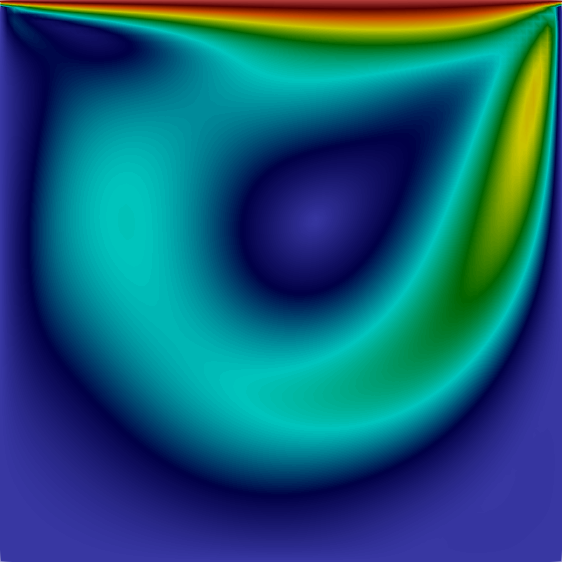
\includegraphics[width=\linewidth]{Figuras/Cavity/Re400.png}
        \caption{$\Rey=400$}
    \end{subfigure}
    \begin{subfigure}{0.32\textwidth}
        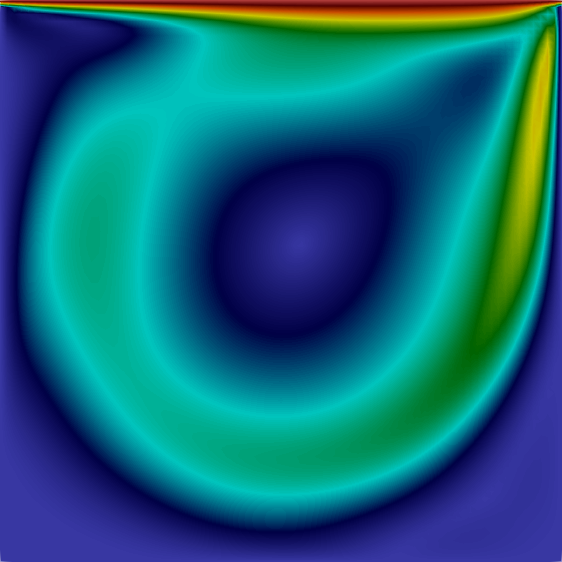
\includegraphics[width=\linewidth]{Figuras/Cavity/Re1000.png}
        \caption{$\Rey=1000$}
    \end{subfigure}
    \begin{subfigure}{0.32\textwidth}
        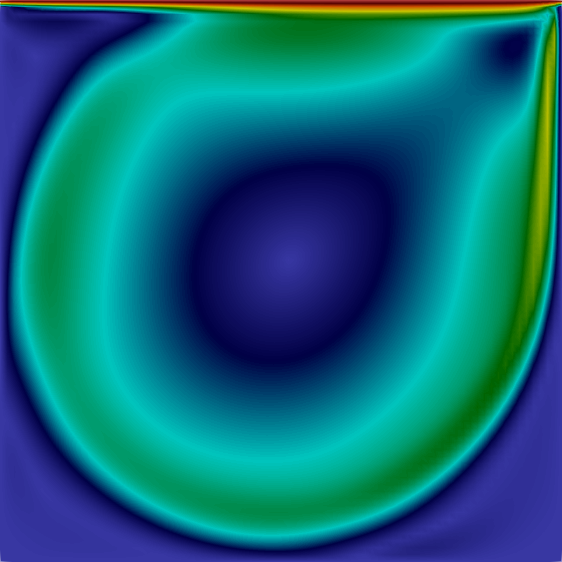
\includegraphics[width=\linewidth]{Figuras/Cavity/Re5000.png}
        \caption{$\Rey=5000$}
    \end{subfigure}
    \begin{subfigure}{0.32\textwidth}
        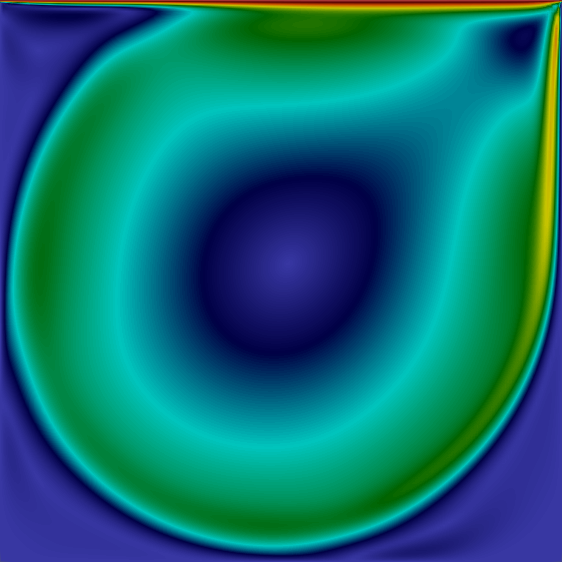
\includegraphics[width=\linewidth]{Figuras/Cavity/Re7500.png}
        \caption{$\Rey=7500$}
    \end{subfigure}
    \begin{subfigure}{0.32\textwidth}
        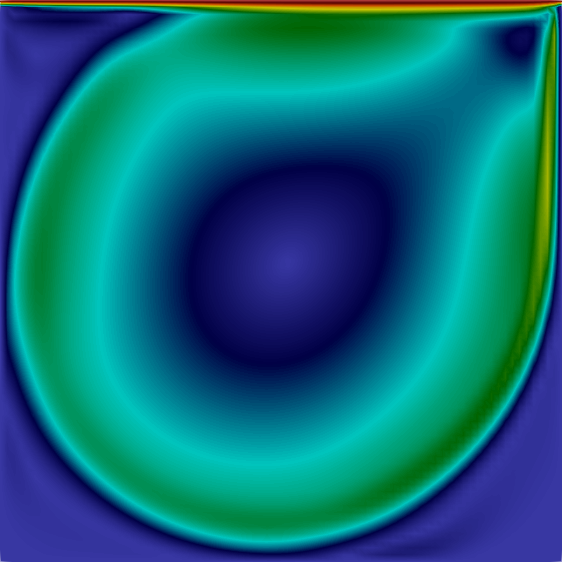
\includegraphics[width=\linewidth]{Figuras/Cavity/Re10000.png}
        \caption{$\Rey=10000$}
    \end{subfigure}
    \begin{subfigure}{0.4\textwidth}
        
\includegraphics[width=\linewidth]{Figuras/Cavity/Legenda.png}
    \end{subfigure}
    \\Fonte: Autoria Própria (\the\year).
    \label{fig:cavity-results2}
\end{figure}

Para todas as simulações conduzidas, percebeu-se que houve uma excelente concordância dos resultados para números de Reynolds baixos, no entanto a simulação VMS de aproximação linear passou a apresentar resultados cada vez mais discrepantes à medida que o número de Reynolds aumentou, enquanto o VMS de aproximação quadrática e o LES apresentaram resultados mais próximos aos de \citeonline{ghia1982high}, sendo que o LES apresentou resultados ligeiramente melhores em relação ao VMS quadrático. Para número de Reynolds muito altos observou-se um leve desvio nos resultados próximos à parede superior da cavidade, o que poderia ser melhorado caso uma discretização mais fina da malha fosse empregada nessa região.

Para comparação da convergência entre os modelos implementados realizou-se um simulação com $\Rey=1000$ partindo de uma condição inicial $\BB{u}=\BB{0}$ em todo o domínio. As medidas de resíduos observadas foram relacionadas à velocidade ($e_u=\norm{\Delta\BB{U}}$) e à pressão ($e_p=\norm{\Delta\BB{P}}$) e a simulação foi conduzida até que um resíduo abaixo de $1\times10^{-8}$ fosse obtido. A Figura \ref{fig:comp-res} apresenta a convergência dos modelos segundo essas medidas.

\begin{figure}[h!]
    \centering
    \caption{Comparação do resíduo da:}
    \begin{subfigure}{\textwidth}
        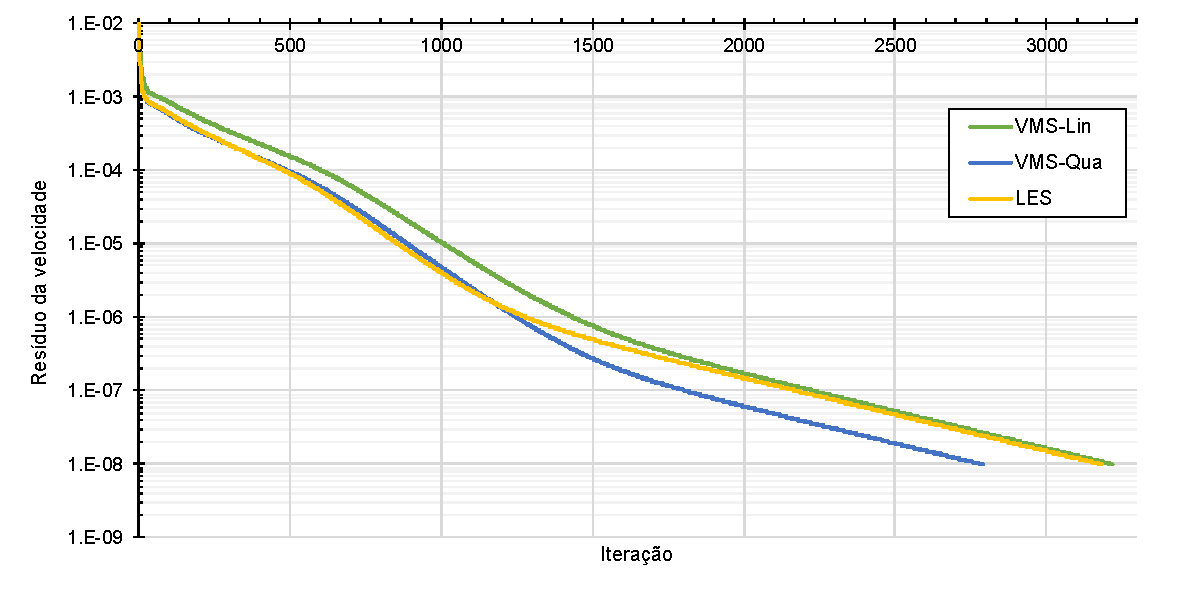
\includegraphics[width=\linewidth]{Figuras/Cavity/resvel.pdf}
        \caption{velocidade.}
    \end{subfigure}
    \begin{subfigure}{\textwidth}
        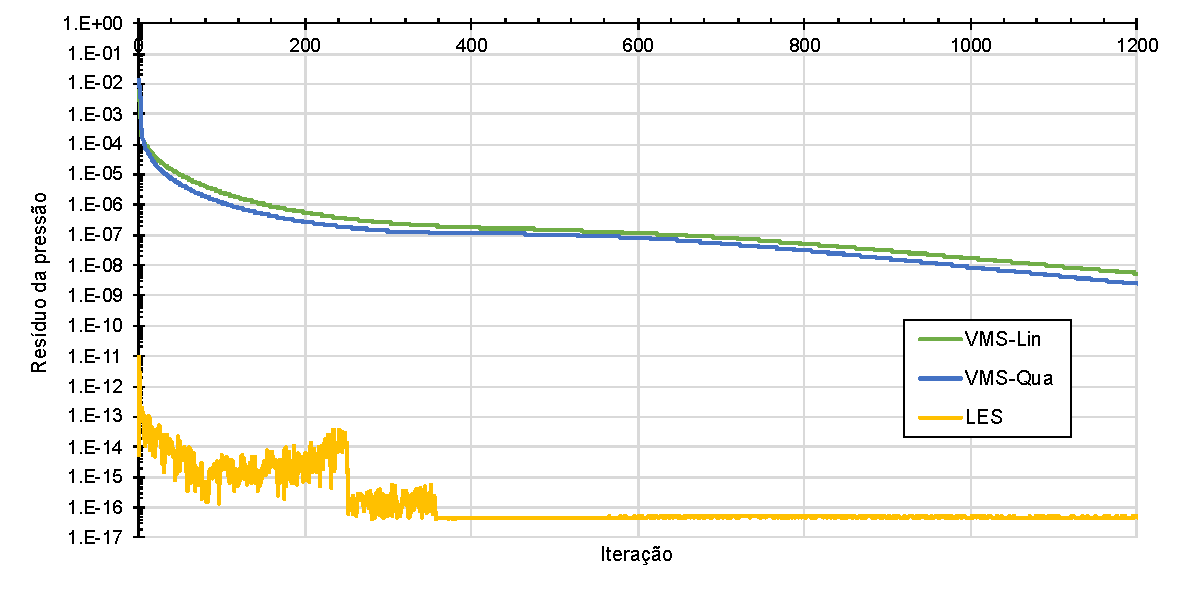
\includegraphics[width=\linewidth]{Figuras/Cavity/respre.pdf}
        \caption{pressão.}
    \end{subfigure}
    \\Fonte: Autoria Própria (\the\year).
    \label{fig:comp-res}
\end{figure}

Também foi observado o tempo necessário para que a convergência fosse atingida. A Tabela \ref{tab:comp-res} apresenta o número de iteração necessárias para que ambas as medidas de erro atingissem a tolerância, o tempo médio por iteração e o tempo total da simulação.

\begin{table}[h!]
    \centering
    \caption{Resultados do estudo de convergência dos métodos.}
    \begin{tabular}{lccc}
        \hline
        Modelo         & número de iterações & tempo por iteração (s) & tempo (min) \\\hline
        VMS linear     & 3218                & 0,650                  & 34,872      \\
        VMS quadrático & 2788                & 3,814                  & 177,260     \\
        LES            & 3182                & 3,494                  & 185,357     \\\hline
    \end{tabular}
    \\Fonte: Autoria Própria (\the\year).
    \label{tab:comp-res}
\end{table}

Observa-se no resíduo da velocidade que todos os métodos tiveram uma convergência mais rápida no início da simulação, pois um fluxo rotacional ainda estava sendo obtido pelos modelos. Após se estabelecer esse fluxo a convergência desacelerou até atingir a tolerância admitida. Já com relação ao resíduo da pressão verifica-se que o modelo LES obteve uma convergência imediata, no entanto a convergência dos demais modelos também foi rápida de tal forma a essa medida não ser o limitante em relação ao tempo de processamento. Ao final do processamento o VMS quadrático foi o que precisou da menor quantidade de iterações para convergir, no entanto, devido à quantidade de graus de liberdade ser maior, seu tempo requerido para cada iteração aumentou, necessitando de um tempo similar ao LES.

Por fim, verificou-se a necessidade da utilização do modelo de turbulência em simulações de malha menos refinada em situação de número de Reynolds elevado. Para isso assumiu-se um problema com $\Rey=10000$, sendo o domínio computacional gerado pela divisão de cada aresta em 20 segmentos, totalizando, assim, 800 elementos finitos triangulares, dispostos de forma estruturada com orientação à esquerda. As simulações foram conduzidas sem a utilização de nenhum modelo de turbulência, seguido dos modelos LES e VMS. Para cada uma das simulações empregou-se elementos de aproximação linear, quadrática e Taylor-Hood P2P1, sendo que para os dois primeiros aplicou-se um estabilizador PSPG, uma vez que esses elementos não possuem estabilidade no campo de pressões. Assim, chegou-se em 441 nós e 1323 DOF para a simulação contendo elementos lineares, 1681 nós e 5043 DOF para quadráticos e 1681 nós e 3803 DOF para P2P1. A simulação foi mantida em um intervalo de tempo $t\in[0,500]$, discretizado em $\Delta t=0,1$, sendo que a condição inicial foi de $\BB{u}=\BB{0}$ em todos os pontos no interior do domínio. A Tabela \ref{tab:comp-res2} apresenta de forma qualitativa os resultados obtidos. O campo de velocidades obtidos para cada simulação no instante $t=500$ é apresentado no Apêndice A.

\begin{table}[h!]
    \centering
    \caption{Comparação dos resultados apresentados em simulação em modelo, com aplicação de LES e de VMS.}
    \begin{tabularx}{\textwidth}{|p{2cm}|p{3cm}|X|}
        \hline
        Tipo de elemento      & Simulação  & Resultado                                                         \\\hline
        \MR{3}{*}{Linear}     & Sem modelo & Sem sentido físico                                                \\\cline{2-3}
                              & LES        & Formação de vórtice com valores espúrios próximos à face superior \\\cline{2-3}
                              & VMS        & Formação de vórtice com variação pequena do campo de velocidades  \\\hline
        \MR{3}{*}{Quadrático} & Sem modelo & Não houve avanço na solução (se manteve na condição inicial)      \\\cline{2-3}
                              & LES        & Formação de vórtice                                               \\\cline{2-3}
                              & VMS        & Formação de vórtice                                               \\\hline
        \MR{3}{*}{P2P1}       & Sem modelo & Divergência                                                       \\\cline{2-3}
                              & LES        & Não atingiu o regime permanente                                   \\\cline{2-3}
                              & VMS        & Formação de vórtice                                               \\\hline
    \end{tabularx}
    \\Fonte: Autoria Própria (\the\year).
    \label{tab:comp-res2}
\end{table}

Logo, verifica-se que as simulações sem a aplicação de modelos de turbulência não foi capaz de simular o comportamento do escoamento. Por outro lado, mesmo em uma situação de malha grosseira, as simulações empregando LES e VMS foram capazes de capturar esse comportamento. No entanto a simulação modelada por LES em elemento P2P1 não atingiu o regime permanente.

%==================================================================================================
\subsubsection{\textit{Taylor-Green Vortex} tridimensional}
%==================================================================================================

Para verificação dos modelos implementados em simulações tridimensionais é possível simular o problema de \textit{Taylor-Green Vortex} (TGV), o qual possui solução analítica, dada por \cite{shapiro1993use}:

\begin{subequations}
    \begin{equation}
        \begin{split}
            &\BB{u}_a(\BB{x},t)=\\
            &-\frac{Ae^{-\nu\lambda^2t}}{k^2+l^2}\begin{bmatrix}
                \lambda l\cos{(kx_1)}\sin{(lx_2)}\sin{(mx_3)}+mk\sin{(kx_1)}\cos{(lx_2)}\cos{(mx_3)} \\
                \lambda k\sin{(kx_1)}\cos{(lx_2)}\sin{(mx_3)}-ml\cos{(kx_1)}\sin{(lx_2)}\cos{(mx_3)} \\
                -(k^2+l^2)\cos{(kx_1)}\cos{(lx_2)}\sin{(mx_3)}
            \end{bmatrix}\text{,}
        \end{split}
    \end{equation}
    \begin{equation}
        p_a=p_s-\rho\frac{u_1^2+u_2+u_3^2}{2}\text{.}
    \end{equation}
\end{subequations}

\noindent em que $k$, $l$ e $m$ são constantes arbitrárias, $\lambda^2=k^2+l^2+m^2$, $A$ é a amplitude da componente $u_3$ e $p_s$ é a pressão do ponto de estagnação.

Para o problema numérico foi considerado um cubo ($\Omega=[-1,1]^3$) simulado nos modelos VMS de aproximação linear e quadrática e o LES utilizando elementos Taylor-Hood P2P1. A malha utilizada na discretização conta com 5802 elementos finitos (conforme ilustrado na Figura \ref{fig:TGV-mesh}), sendo 5580 graus de liberdade para VMS linear, 37600 pra VMS quadrático e 29595 para LES.

\begin{figure}[h!]
    \centering
    \caption{Malha utilizada para a simulação de TGV.}
    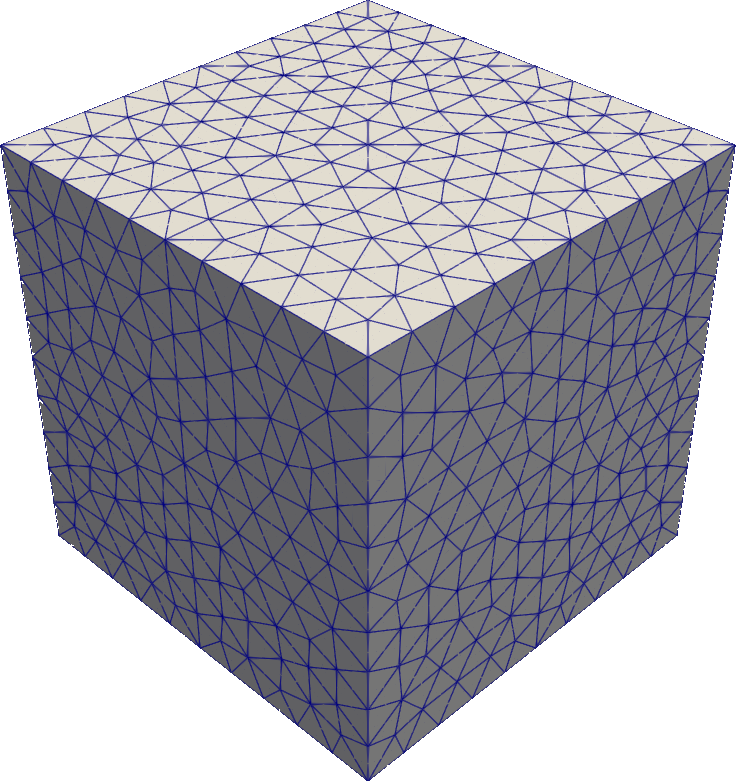
\includegraphics[width=0.4\linewidth]{Figuras/taylor-green/mesh.png}
    \\Fonte: Autoria Própria (\the\year).
    \label{fig:TGV-mesh}
\end{figure}

Como condição inicial impôs-se acelerações, velocidade e pressões iguais à solução analítica com $t=0$ e como condições de contorno aplicou-se velocidades iguais à analítica em toda a fronteira e $p=0$ no centro do domínio. Os valores dos parâmetros foram $k=l=m=\pi$ e $A=\nu=\rho=1$, sendo o período analisado de $t\in[0,0.2]$ com um passo de tempo de $\Delta t=0.001$.

Sendo assim, a Figura \ref{fig:TGV-results} apresenta os valores do campo de velocidades nas linhas $x_2=x_3=0$ ($l1$), $x_1=x_3=0$ ($l2$) e $x_1=x_2=0$ ($l3$) para os instantes $t=0$, $t=0.05$ e $t=0.2$ para todos os modelos considerados.

\begin{figure}[h!]
    \centering
    \caption{Velocidades obtidas na a simulação de TGV em:}
    \begin{subfigure}{0.42\textwidth}
        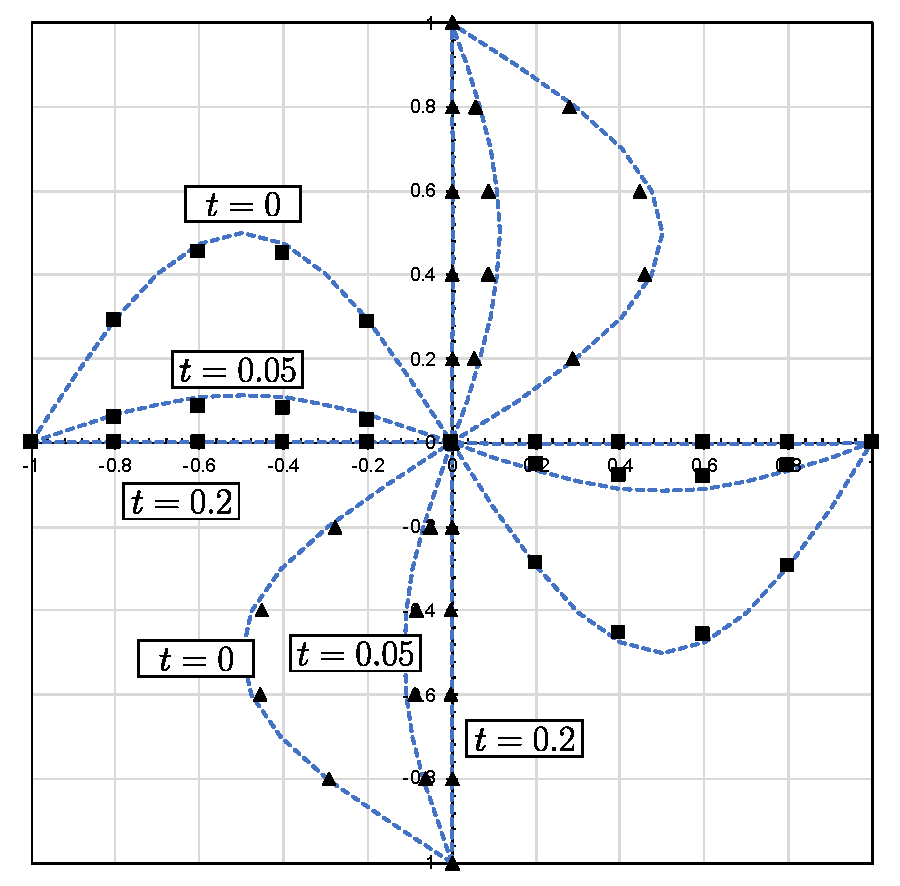
\includegraphics[width=\linewidth]{Figuras/taylor-green/VMS-Lin.pdf}
        \caption{$l1$ e $l2$ para VMS linear.}
    \end{subfigure}
    \begin{subfigure}{0.42\textwidth}
        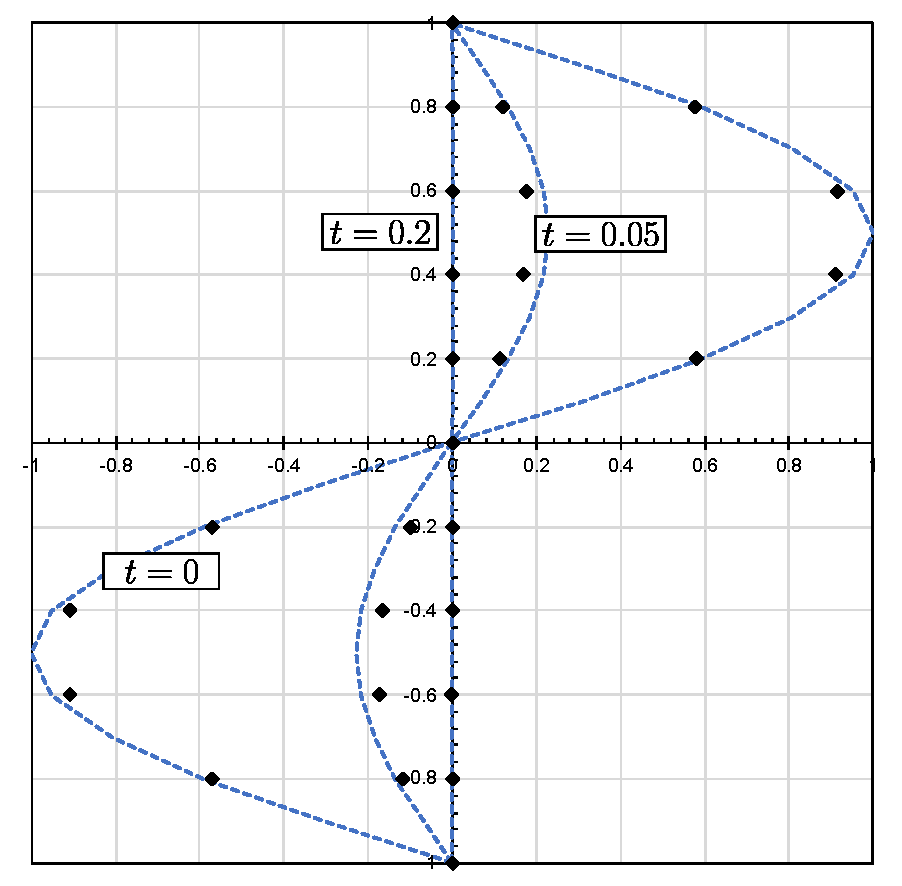
\includegraphics[width=\linewidth]{Figuras/taylor-green/VMS-Lin-uz.pdf}
        \caption{$l3$ para VMS linear.}
    \end{subfigure}
    \begin{subfigure}{0.42\textwidth}
        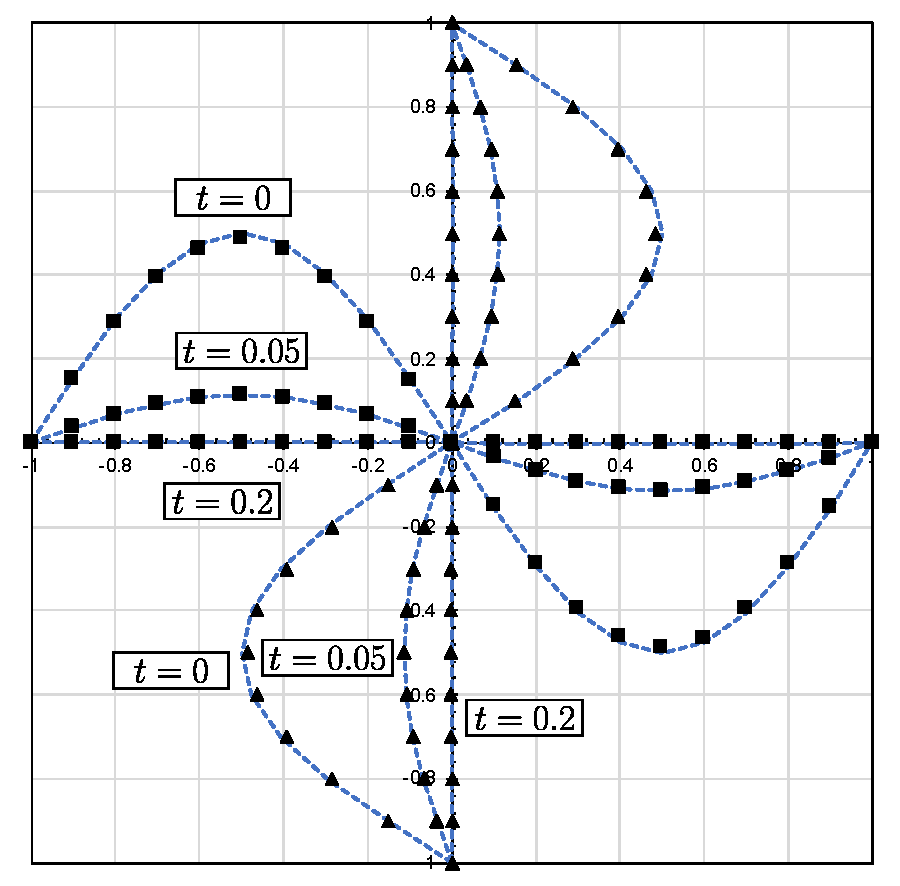
\includegraphics[width=\linewidth]{Figuras/taylor-green/VMS-Qua.pdf}
        \caption{$l1$ e $l2$ para VMS quadrático.}
    \end{subfigure}
    \begin{subfigure}{0.42\textwidth}
        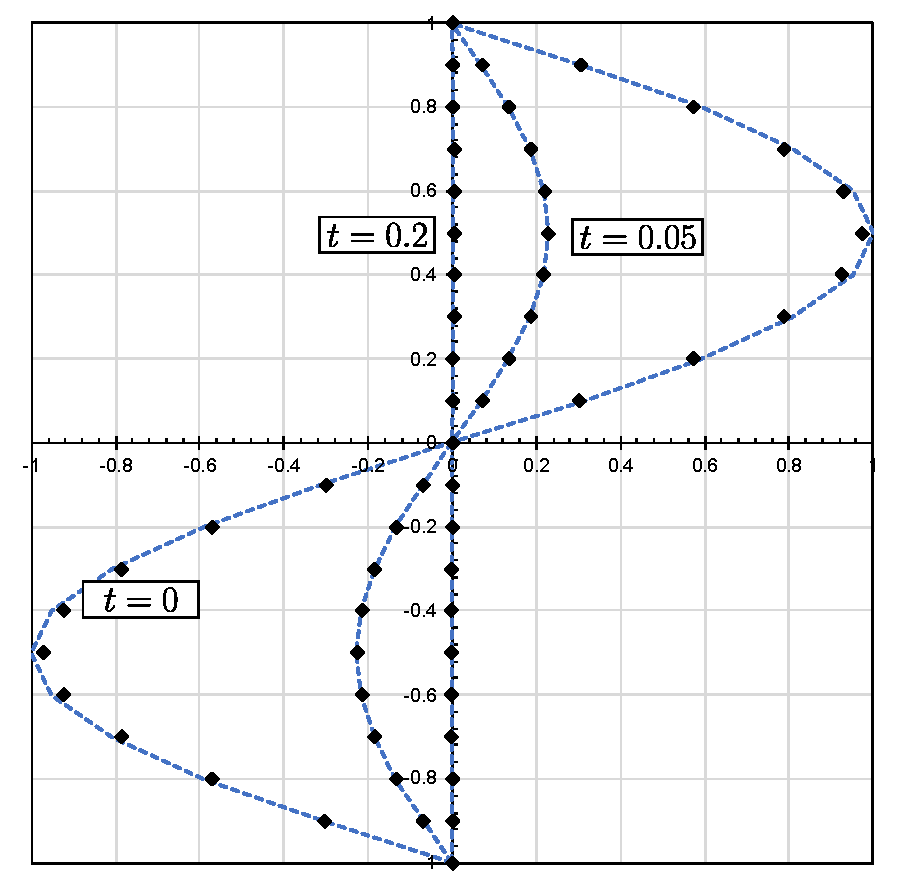
\includegraphics[width=\linewidth]{Figuras/taylor-green/VMS-Qua-uz.pdf}
        \caption{$l3$ para VMS quadrático.}
    \end{subfigure}
    \begin{subfigure}{0.42\textwidth}
        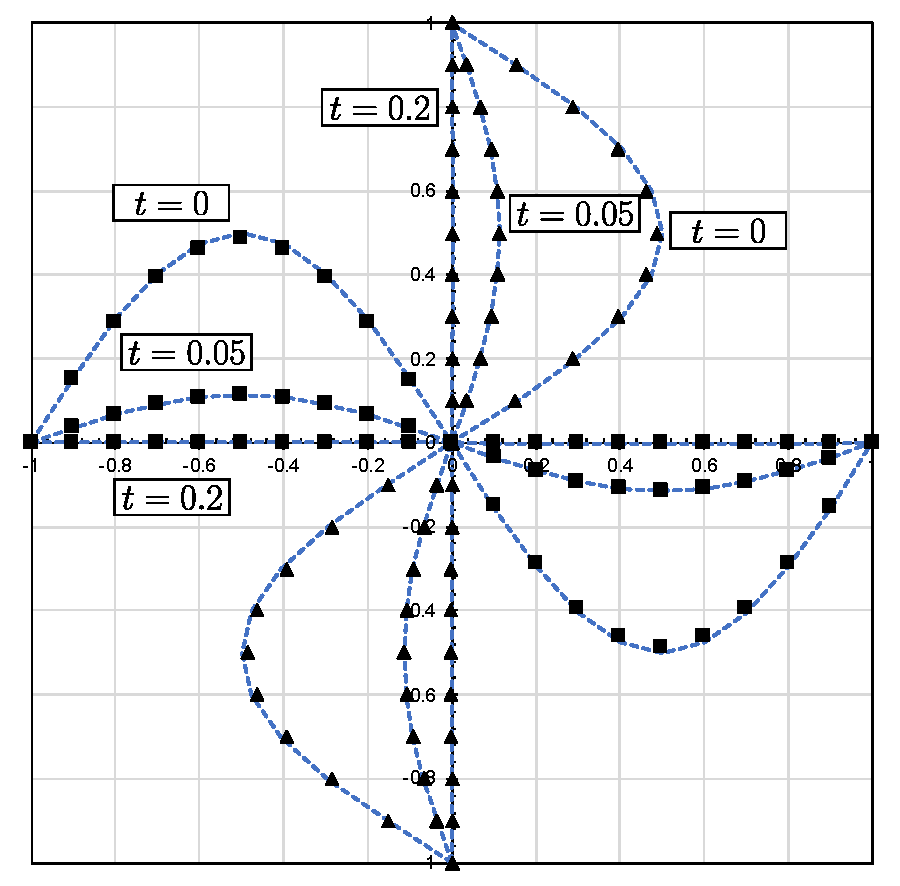
\includegraphics[width=\linewidth]{Figuras/taylor-green/LES.pdf}
        \caption{$l1$ e $l2$ para LES.}
    \end{subfigure}
    \begin{subfigure}{0.42\textwidth}
        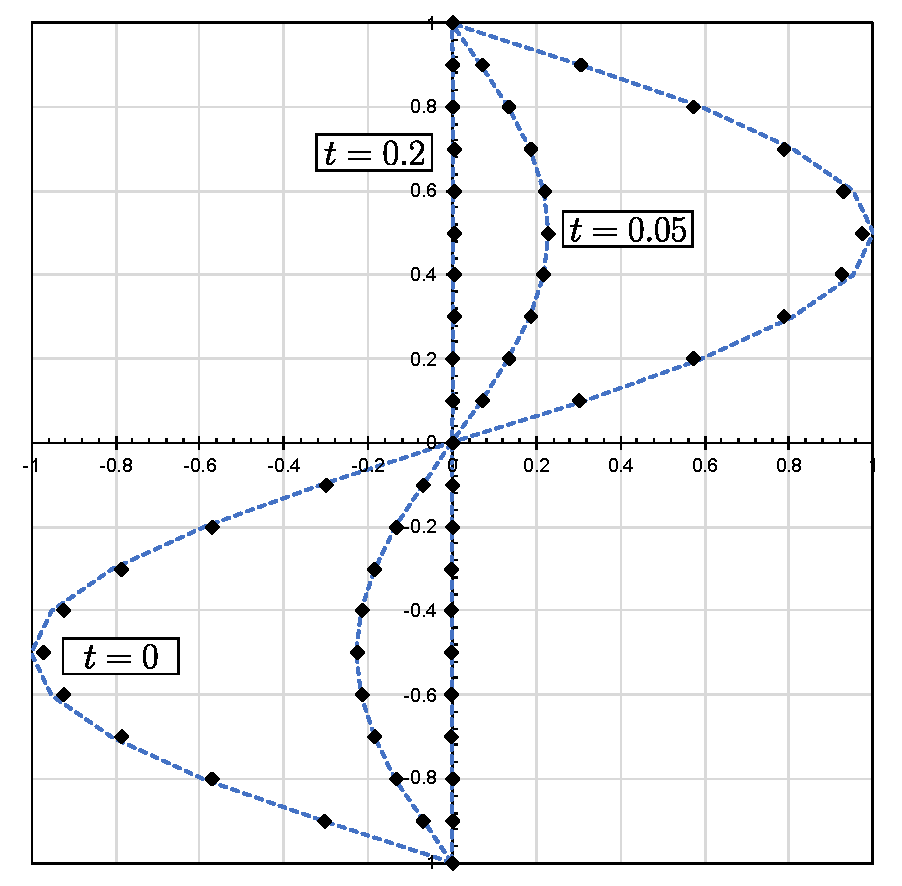
\includegraphics[width=\linewidth]{Figuras/taylor-green/LES-uz.pdf}
        \caption{$l3$ para LES.}
    \end{subfigure}
    \begin{subfigure}{0.42\textwidth}
        
\includegraphics[width=\linewidth]{Figuras/taylor-green/legenda.pdf}
    \end{subfigure}
    \\Fonte: Autoria Própria (\the\year).
    \label{fig:TGV-results}
\end{figure}

Para comparação com a solução analítica, tomou-se a medida do erro em $L^2$, expresso por \cite{dumon2011proper}:

\begin{equation}
    \norm{\BB{e}}=\norm{\BB{u}-\BB{u}_a}_{L^\infty(L^2(\Omega))}=\max_{0<t\leq T}{\left[\int_\Omega{\norm{\BB{u}-\BB{u}_a}^2d\Omega}\right]}\text{,}
\end{equation}

\noindent o qual é representado ao longo do tempo de acordo com a Figura \ref{fig:TGV-L2}:

\begin{figure}[h!]
    \centering
    \caption{Medidas de $L^2$ ao longo do tempo.}
    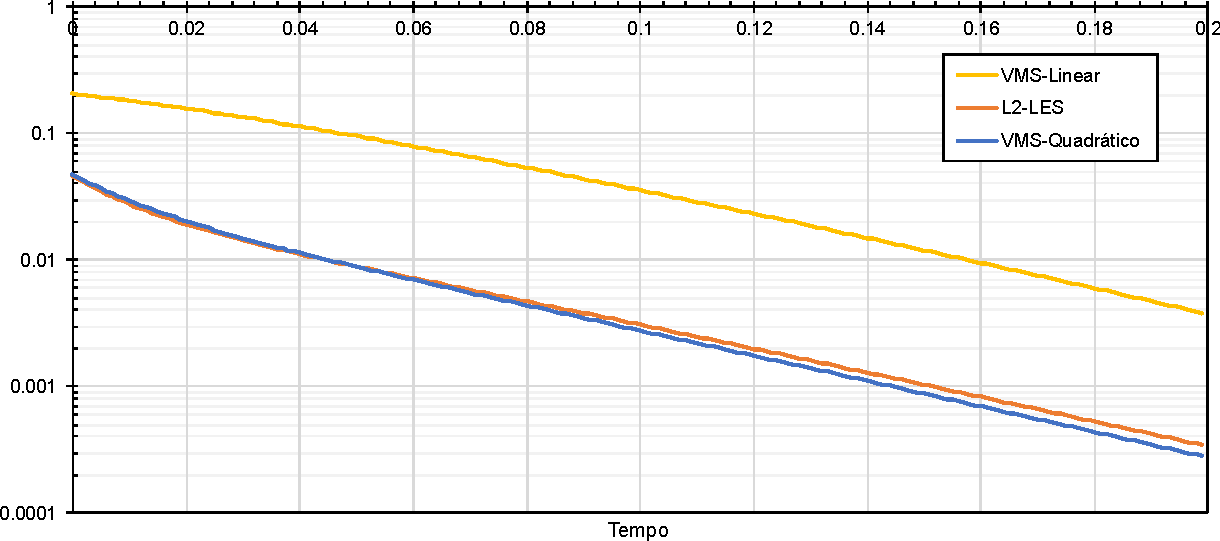
\includegraphics[width=\linewidth]{Figuras/taylor-green/L2.pdf}
    \\Fonte: Autoria Própria (\the\year).
    \label{fig:TGV-L2}
\end{figure}

Assim, observa-se que para o problema estudado, tanto as simulações VMS de aproximação quadrática quanto LES com elemento P2P1 apresentaram boa concordância com o resultado analítico, sendo que ambos apresentaram erros muito próximos entre si, enquanto o VMS de aproximação linear já apresentou um erro maior. Analisando o instante de tempo $t=0.1$ obteve-se um erro $L^2$ de $3,55\times 10^{-2}$, $2,77\times 10^{-3}$ e $3,07\times 10^{-3}$ para as simulações VMS linear, quadrático e LES, respectivamente. Ao verificar a ordem da medida do erro, observa-se que estes valores encontram-se próximos ao obtido por \citeonline{zapata2023parallel}. Realizando uma regressão exponencial do tipo \[\norm{\BB{e}}=a\cdot10^{mt}\] para $t\geq 0,1$, encontra-se $m=-9,80$, $m=-10,01$ e $m=-9,60$ para os respectivos modelos.

%==================================================================================================
\subsubsection{Escoamento sobre um cilindro}
%==================================================================================================

Para o seguinte problema considerou-se um cilindro circular de raio $R=0,5$ em um domínio retangular $\Omega=[0,112R]\times[0,100R]$, sendo o centro do cilindro posicionado sobre o ponto $(36,50)R$. As condições de contorno consideradas foram de entrada na face esquerda ($x_1=0$) do domínio ($\BB{u}=\{u_\infty,0\}^T$), condição de velocidade vertical nula nas faces inferior e superior ($u_2=0$ em $x_2=0$ e $x_2=100R$) e pressão nula no ponto $(112,100)R$. Como condição inicial aplicou-se uma velocidade $\BB{u}=\{u_\infty,0\}^T$ em todo o domínio. A densidade do fluido foi de $\rho=1$ com viscosidade $\nu=0,01$ e uma velocidade $u_\infty=1$, que, ao considerar o comprimento característico como o diâmetro do cilindro, obtém-se $\Rey=100$.

Para a simulação numérica considerou-se a malha apresentada na Figura \ref{fig:cyl-mesh}, a qual possui 4656 elementos finitos. Assim, estudou-se o escoamento em situação onde não se aplicou nenhum modelo de turbulência, seguido da aplicação dos modelos LES e VMS. Todas as simulações foram conduzidas utilizando os elementos de aproximação linear, quadrática e Taylor-Hood P2P1. Para os elementos linear e quadrático aplicou-se em todos os casos o estabilizador PSPG para obtenção de resultados consistentes. O problema discretizado possui 7263 graus de liberdade para elemento linear, 28494 para elemento quadrático e 21417 para P2P1. O intervalo de tempo foi de $t\in[0,200]$ com passos de $\Delta t=0,1$.

\begin{figure}[h!]
    \centering
    \caption{Malha utilizada para a simulação de escoamento sobre um cilindro.}
    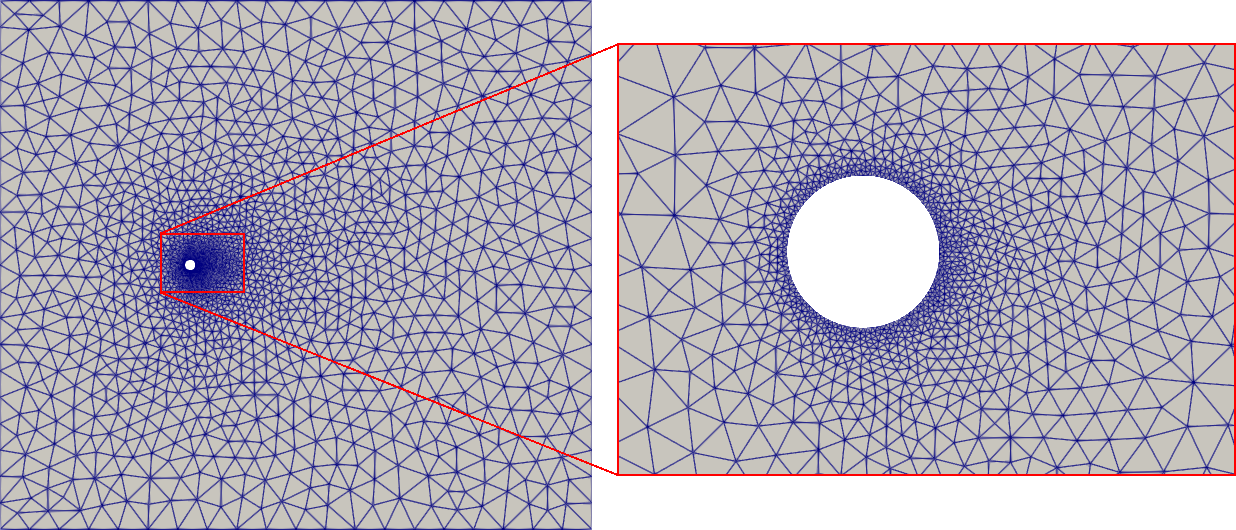
\includegraphics[width=\linewidth]{Figuras/cylinder/analise2/mesh.png}
    \\Fonte: Autoria Própria (\the\year).
    \label{fig:cyl-mesh}
\end{figure}

Para análise dos resultados determinou-se os coeficientes de arrasto (\textit{Drag} - $C_D$) e de sustentação (\textit{Lift} - $C_L$), dados respectivamente por:

\begin{subequations}
    \begin{equation}
        C_D=\frac{2F_D}{\rho\norm{\BB{u}_\infty}^2L}\text{ e}
    \end{equation}
    \begin{equation}
        C_L=\frac{2F_L}{\rho\norm{\BB{u}_\infty}^2L}\text{,}
    \end{equation}
\end{subequations}

\noindent em que $F_D$ e $F_L$ são as forças de arrasto e de sustentação, calculados como:

\begin{subequations}
    \begin{equation}
        F_D=\int_{\Gamma_S}{\sigma_{1j}n_jd\Gamma_S}\text{ e}
    \end{equation}
    \begin{equation}
        F_L=\int_{\Gamma_S}{\sigma_{2j}n_jd\Gamma_S}\text{,}
    \end{equation}
\end{subequations}

\noindent sendo $\Gamma_S$ a fronteira do cilindro e $\BB{n}$ o vetor normal à $\Gamma_S$.

Outro parâmetro possível de se verificar é o número de Strouhal ($\Str$), que se trata de um número adimensional que busca relacionar a frequência de oscilação devido à formação de vórtices e a velocidade do fluido. Esse parâmetro pode ser determinado por:

\begin{equation}
    \Str=\frac{f_vL}{\norm{\BB{u}_\infty}}\text{,}
\end{equation}

\noindent sendo $f_v$ a frequência de desprendimento de vórtices.

As Figuras \ref{fig:cyl-draglift-None}, \ref{fig:cyl-draglift-LES} e \ref{fig:cyl-draglift-VMS} apresentam os coeficientes de arrasto e de sustentação obtidos em todas as simulações. Os campos de velocidades e de pressões atuantes no cilindro no instante $t=120$ são apresentados no Apêndice B.

\begin{figure}[h!]
    \centering
    \caption{Valores ao longo do tempo na simulação sem modelo de:}
    \begin{subfigure}{.49\textwidth}
        \centering
        \includegraphics[width=\linewidth]{Figuras/cylinder/analise2/none-drag.pdf}
        \caption{coeficiente de arrasto.}
    \end{subfigure}
    \begin{subfigure}{.49\textwidth}
        \centering
        \includegraphics[width=\linewidth]{Figuras/cylinder/analise2/none-lift.pdf}
        \caption{coeficiente de sustentação.}
    \end{subfigure}
    \begin{subfigure}{\textwidth}
        \centering
        \includegraphics[width=.4\linewidth]{Figuras/cylinder/analise2/legenda.pdf}
    \end{subfigure}
    \\Fonte: Autoria Própria (\the\year).
    \label{fig:cyl-draglift-None}
\end{figure}

\begin{figure}[h!]
    \centering
    \caption{Valores ao longo do tempo na simulação LES de:}
    \begin{subfigure}{.49\textwidth}
        \centering
        \includegraphics[width=\linewidth]{Figuras/cylinder/analise2/LES-drag.pdf}
        \caption{coeficiente de arrasto.}
    \end{subfigure}
    \begin{subfigure}{.49\textwidth}
        \centering
        \includegraphics[width=\linewidth]{Figuras/cylinder/analise2/LES-lift.pdf}
        \caption{coeficiente de sustentação.}
    \end{subfigure}
    \begin{subfigure}{\textwidth}
        \centering
        \includegraphics[width=.4\linewidth]{Figuras/cylinder/analise2/legenda.pdf}
    \end{subfigure}
    \\Fonte: Autoria Própria (\the\year).
    \label{fig:cyl-draglift-LES}
\end{figure}

\begin{figure}[h!]
    \centering
    \caption{Valores ao longo do tempo na simulação VMS de:}
    \begin{subfigure}{.49\textwidth}
        \centering
        \includegraphics[width=\linewidth]{Figuras/cylinder/analise2/VMS-drag.pdf}
        \caption{coeficiente de arrasto.}
    \end{subfigure}
    \begin{subfigure}{.49\textwidth}
        \centering
        \includegraphics[width=\linewidth]{Figuras/cylinder/analise2/VMS-lift.pdf}
        \caption{coeficiente de sustentação.}
    \end{subfigure}
    \begin{subfigure}{\textwidth}
        \centering
        \includegraphics[width=.4\linewidth]{Figuras/cylinder/analise2/legenda.pdf}
    \end{subfigure}
    \\Fonte: Autoria Própria (\the\year).
    \label{fig:cyl-draglift-VMS}
\end{figure}

Os valores da média e da amplitude dos coeficientes de arrasto e de sustentação após o escoamento atingir o equilíbrio dinâmico, assim como o número de Strouhal, são apresentados na Tabela \ref{tab:cyl-res}.

\begin{table}[h!]
    \centering
    \newcommand{\celc}{\multicolumn{1}{c}}
    \newcommand{\ccelc}{\multicolumn{2}{c}}
    \caption{Valores das propriedades dos coeficientes de arrasto e de sustentação para os modelos analisados.}
    \begin{tabular}{llllllll}
        \hline
        \MR{2}{*}{Param.}    & \celc{\MR{2}{*}{Modelo}} & \ccelc{Linear} & \ccelc{Quadrático} & \ccelc{Taylor-Hood}                                           \\\cline{3-8}
                             & \celc{}                  & \celc{Drag}    & \celc{Lift}        & \celc{Drag}         & \celc{Lift} & \celc{Drag} & \celc{Lift} \\\hline
        \MR{3}{*}{Amplitude} & Nenhum                   & 0,0102         & 0,3383             & 0,0109              & 0,3436      & 0,0094      & 0,3219      \\
                             & VMS                      & 0,0101         & 0,3333             & 0,0108              & 0,3411      & 0,0088      & 0,3114      \\
                             & LES                      & 0,0101         & 0,3365             & 0,0107              & 0,3417      & 0,0092      & 0,3200      \\\hline
        \MR{3}{*}{Média}     & Nenhum                   & 1,3772         & -0,0006            & 1,3808              & -0,0080     & 1,3209      & -0,0032     \\
                             & VMS                      & 1,3561         & 0,0046             & 1,3620              & -0,0007     & 1,2939      & -0,0083     \\
                             & LES                      & 1,3760         & -0,0003            & 1,3794              & -0,0031     & 1,3199      & -0,0007     \\\hline
        \MR{3}{*}{Strouhal}  & Nenhum                   & \ccelc{0,1594} & \ccelc{0,1623}     & \ccelc{0,1627}                                                \\
                             & VMS                      & \ccelc{0,1588} & \ccelc{0,1634}     & \ccelc{0,1649}                                                \\
                             & LES                      & \ccelc{0,1590} & \ccelc{0,1614}     & \ccelc{0,1629}                                                \\\hline
    \end{tabular}
    \\Fonte: Autoria Própria (\the\year).
    \label{tab:cyl-res}
\end{table}

Comparando-se os números de Strouhal calculados com aqueles obtidos por \citeonline{fernandes2020tecnica}, que obteve, para a mesma geometria de domínio e mesmas condições de contorno, um $\Str=0,165$ e amplitude do coeficiente de sustentação de 0,3422, \citeonline{tezduyar1992incompressible}, os quais verificaram $\Str$ entre 0,166 e 0,170, \citeonline{najafi2012meshless}, com valor de 0,182, e \citeonline{codina2006numerical}, com velores entre 0,177 e 0,184. As variações observadas entre os números de Strouhal dos diferentes autores podem ser devidas às diferenças nas dimensões dos domínios utilizados, assim como as diferentes condições de contorno aplicadas por cada um. No entanto ainda observa-se que em todos os casos os valores calculados nas simulações ainda são bem próximos. Já com relação à amplitude do coeficiente de sustentação, observa-se que as simulações utilizando elementos quadráticos obtiveram melhor concordância com a obtida por \citeonline{fernandes2020tecnica}. A mínima diferença observada entre os parâmetros calculados em uma simulação sem aplicação de modelo e aquelas que aplicam os modelos VMS e LES, deve-se ao fato do número de Reynolds ser muito baixo, pois, como apontado por \citeonline{fernandes2020tecnica}, esse tipo de escoamento (com $\Rey$ entre 50 e 200) apresenta a formação de vórtices laminares, denominada de esteira de Von Kárman. Para uma verificação mais precisa dessa influência, deve-se partir para uma análise tridimensional com número de Reynolds superiores à 200. Em termos de comparação entre os diferentes tipos de aproximação, verifica-se que tanto os elementos lineares e quadráticos atingiram um regime permanente próximos, enquanto o elemento P2P1 apresentou um amortecimento excessivo, tanto no coeficiente de arrasto, quanto no de sustentação. Já realizando uma comparação dos modelos entre si, verifica-se que em todos os casos o coeficiente de sustentação se manteve inalterado, enquanto o coeficiente de arrasto resultou em uma média menor em relação à simulação LES e sem modelo, porém, mantendo os demais parâmetros muito próximos.

%Vale observar ainda que a simulação VMS linear apresentou um amortecimento menor em relação ao início das oscilações, porém converge para valores muito próximos ao quadrático ao longo do tempo. Já a simulação LES inicia sua oscilação próxima ao VMS quadrático, entretanto com uma média de oscilação menor que a do VMS, em especial ao se observar o coeficiente de arrasto. Tal efeito pode ser devido ao relatado por \citeonline{germano1991dynamic,hughes2000large}, que apontam a ocorrência de um amortecimento excessivo provocado pelo tensor SGS de Smagorinsky.
%==================================================================================================
\subsection{Exemplos Numéricos} \label{ExemplosMT}
%==================================================================================================

Na presente seção serão apresentadas algumas simulações realizadas utilizando os modelos VMS e LES, com a finalidade de validar os modelos implementados.

%==================================================================================================
\subsubsection{Cavidade bidimensional}
%==================================================================================================

A primeira simulação é um problema comumente utilizado na literatura como \textit{benchmark}, o qual trata-se de uma cavidade quadrada ($\Omega=[-1,1]^2$) com paredes aderentes, onde o fluido encontra-se confinado e sujeito a uma velocidade prescrita $\BB{u}_\infty$ ocasionada devido ao deslizamento de uma parede na face superior da cavidade. Nesse sentido serão observados os efeitos provocados no fluido devido à diferentes números de Reynolds, o qual é calculado por meio da equação \ref{eq:Reynolds}:

\begin{equation}
    \Rey=\frac{\rho L\norm{\BB{u}_\infty}}{\mu}\text{,}
    \label{eq:Reynolds}
\end{equation}

\noindent em que $L$ é o comprimento característico, que no caso analisado é igual ao lado da cavidade. Dessa forma considera-se uma velocidade constante para todas as análises de $\BB{u}_\infty=\{1,0\}^T$, sendo os diferentes números de Reynolds obtidos pela variação da viscosidade do fluido. A Figura \ref{fig:cavity} apresenta esquematicamente o problema simulado.

\begin{figure}[h!]
    \centering
    \caption{Desenho esquemático do problema de cavidade.}
    \includegraphics[width=.35\linewidth]{Figuras/Cavity/cavidade.pdf}
    \\Fonte: Autoria Própria (\the\year).
    \label{fig:cavity}
\end{figure}

Pelo fato do problema possuir apenas fronteiras do tipo Dirichlet, o condicionamento da solução do campo de pressões é garantido pela aplicação de uma condição de pressão nula no vértice superior direito da cavidade, conforme visto na figura acima.  Também se observa que existe uma descontinuidade nas condições de contorno no encontro entre as paredes da cavidade e seu topo, podendo ser consideradas velocidades nulas ou igual à velocidade do topo. No problema em questão considerou-se que a velocidade nesse ponto é igual à $\BB{u}_\infty$.

A malha de elementos finitos foi feita pela subdivisão do domínio em 20000 elementos dispostos de maneira estruturada com orientação à esquerda, conforme observado na Figura \ref{fig:cavity_disc}. O número de graus de liberdade para a simulação VMS de aproximação linear, quadrática e LES são 30603, 121203 e 91003, respectivamente. Os parâmetros utilizados foram $\rho=1$ para todas as análises, $\mu=0,02$, $\mu=5\times10^{-3}$, $\mu=2\times10^{-3}$, $\mu=4\times10^{-4}$, $\mu=2,6667\times10^{-4}$ e $\mu=2\times10^{-4}$, resultando em $\Rey=100$, $\Rey=400$, $\Rey=1000$, $\Rey=5000$, $\Rey=7500$ e $\Rey=10000$, respectivamente. Os modelos utilizados foram o VMS com aproximação linear e quadrática e o LES com elementos de Taylor-Hood P2P1 e $C_S=0,10$. O passo de tempo em todos os casos foi de $\Delta t=0,1$ e a simulação foi mantida até que a estacionariedade dos parâmetros do fluxo fosse alcançada.

\begin{figure}[h!]
    \centering
    \caption{Malha considerada para o problema de cavidade.}
    \includegraphics[width=.6\linewidth]{Figuras/Cavity/mesh.pdf}
    \\Fonte: Autoria Própria (\the\year).
    \label{fig:cavity_disc}
\end{figure}

Como o problema apresenta características de um escoamento quase-estático, a parcela dos termos inerciais foram desprezados em ambos os modelos de turbulência. Além disso, os resultados adquiridos para um determinado número de Reynolds foram aplicados como valores iniciais para a determinação dos resultados para a próxima análise.

Os resultados obtidos foram comparados com aqueles apresentados por \citeonline{ghia1982high}. A Figura \ref{fig:cavity-results} apresenta os valores do campo de velocidades sobre as linhas médias da cavidade ($x_1=0$ e $x_2=0$).

\begin{figure}[h!]
    \centering
    \caption{Valores do campo de velocidades sobre as linhas médias da cavidade.}
    \begin{subfigure}{0.4\textwidth}
        \includegraphics[width=\linewidth]{Figuras/Cavity/Re100.pdf}
        \caption{$\Rey=100$}
    \end{subfigure}
    \begin{subfigure}{0.4\textwidth}
        \includegraphics[width=\linewidth]{Figuras/Cavity/Re400.pdf}
        \caption{$\Rey=400$}
    \end{subfigure}
    \begin{subfigure}{0.4\textwidth}
        \includegraphics[width=\linewidth]{Figuras/Cavity/Re1000.pdf}
        \caption{$\Rey=1000$}
    \end{subfigure}
    \begin{subfigure}{0.4\textwidth}
        \includegraphics[width=\linewidth]{Figuras/Cavity/Re5000.pdf}
        \caption{$\Rey=5000$}
    \end{subfigure}
    \begin{subfigure}{0.4\textwidth}
        \includegraphics[width=\linewidth]{Figuras/Cavity/Re7500.pdf}
        \caption{$\Rey=7500$}
    \end{subfigure}
    \begin{subfigure}{0.4\textwidth}
        \includegraphics[width=\linewidth]{Figuras/Cavity/Re10000.pdf}
        \caption{$\Rey=10000$}
    \end{subfigure}
    \begin{subfigure}{\textwidth}
        \includegraphics[width=\linewidth]{Figuras/Cavity/Legenda.pdf}
    \end{subfigure}
    \\Fonte: Autoria Própria (\the\year).
    \label{fig:cavity-results}
\end{figure}

A Figura \ref{fig:cavity-results2} apresenta o campo de velocidades na cavidade após o escoamento atingir seu estado estacionário.

\begin{figure}[h!]
    \centering
    \caption{Campo de velocidades em regime estacionário na cavidade.}
    \begin{subfigure}{0.32\textwidth}
        \includegraphics[width=\linewidth]{Figuras/Cavity/Re100.png}
        \caption{$\Rey=100$}
    \end{subfigure}
    \begin{subfigure}{0.32\textwidth}
        \includegraphics[width=\linewidth]{Figuras/Cavity/Re400.png}
        \caption{$\Rey=400$}
    \end{subfigure}
    \begin{subfigure}{0.32\textwidth}
        \includegraphics[width=\linewidth]{Figuras/Cavity/Re1000.png}
        \caption{$\Rey=1000$}
    \end{subfigure}
    \begin{subfigure}{0.32\textwidth}
        \includegraphics[width=\linewidth]{Figuras/Cavity/Re5000.png}
        \caption{$\Rey=5000$}
    \end{subfigure}
    \begin{subfigure}{0.32\textwidth}
        \includegraphics[width=\linewidth]{Figuras/Cavity/Re7500.png}
        \caption{$\Rey=7500$}
    \end{subfigure}
    \begin{subfigure}{0.32\textwidth}
        \includegraphics[width=\linewidth]{Figuras/Cavity/Re10000.png}
        \caption{$\Rey=10000$}
    \end{subfigure}
    \begin{subfigure}{0.4\textwidth}
        \includegraphics[width=\linewidth]{Figuras/Cavity/Legenda.png}
    \end{subfigure}
    \\Fonte: Autoria Própria (\the\year).
    \label{fig:cavity-results2}
\end{figure}

Para todas as simulações conduzidas, percebeu-se que houve uma excelente concordância dos resultados para números de Reynolds baixos, no entanto a simulação VMS de aproximação linear passou a apresentar resultados cada vez mais discrepantes à medida que o número de Reynolds aumentou, enquanto o VMS de aproximação quadrática e o LES apresentaram resultados mais próximos aos de \citeonline{ghia1982high}, sendo que o LES apresentou resultados ligeiramente melhores em relação ao VMS quadrático. Para número de Reynolds muito altos observou-se um leve desvio nos resultados próximos à parede superior da cavidade, o que poderia ser melhorado caso uma discretização mais fina da malha fosse empregada nessa região.

Para comparação da convergência entre os modelos implementados realizou-se um simulação com $\Rey=1000$ partindo de uma condição inicial $\BB{u}=\BB{0}$ em todo o domínio. As medidas de resíduos observadas foram relacionadas à velocidade ($e_u=\norm{\Delta\BB{U}}$) e à pressão ($e_p=\norm{\Delta\BB{P}}$) e a simulação foi conduzida até que um resíduo abaixo de $1\times10^{-8}$ fosse obtido. A Figura \ref{fig:comp-res} apresenta a convergência dos modelos segundo essas medidas.

\begin{figure}[h!]
    \centering
    \caption{Comparação do resíduo da:}
    \begin{subfigure}{\textwidth}
        \includegraphics[width=\linewidth]{Figuras/Cavity/resvel.pdf}
        \caption{velocidade.}
    \end{subfigure}
    \begin{subfigure}{\textwidth}
        \includegraphics[width=\linewidth]{Figuras/Cavity/respre.pdf}
        \caption{pressão.}
    \end{subfigure}
    \\Fonte: Autoria Própria (\the\year).
    \label{fig:comp-res}
\end{figure}

Também foi observado o tempo necessário para que a convergência fosse atingida. A Tabela \ref{tab:comp-res} apresenta o número de iteração necessárias para que ambas as medidas de erro atingissem a tolerância, o tempo médio por iteração e o tempo total da simulação.

\begin{table}[h!]
    \centering
    \caption{Resultados do estudo de convergência dos métodos.}
    \begin{tabular}{lccc}
        \hline
        Modelo         & número de iterações & tempo por iteração (s) & tempo (min) \\\hline
        VMS linear     & 3218                & 0,650                  & 34,872      \\
        VMS quadrático & 2788                & 3,814                  & 177,260     \\
        LES            & 3182                & 3,494                  & 185,357     \\\hline
    \end{tabular}
    \\Fonte: Autoria Própria (\the\year).
    \label{tab:comp-res}
\end{table}

Observa-se no resíduo da velocidade que todos os métodos tiveram uma convergência mais rápida no início da simulação, pois um fluxo rotacional ainda estava sendo obtido pelos modelos. Após se estabelecer esse fluxo a convergência desacelerou até atingir a tolerância admitida. Já com relação ao resíduo da pressão verifica-se que o modelo LES obteve uma convergência imediata, no entanto a convergência dos demais modelos também foi rápida de tal forma a essa medida não ser o limitante em relação ao tempo de processamento. Ao final do processamento o VMS quadrático foi o que precisou da menor quantidade de iterações para convergir, no entanto, devido à quantidade de graus de liberdade ser maior, seu tempo requerido para cada iteração aumentou, necessitando de um tempo similar ao LES.

Por fim, verificou-se a necessidade da utilização do modelo de turbulência em simulações de malha menos refinada em situação de número de Reynolds elevado. Para isso assumiu-se um problema com $\Rey=10000$, sendo o domínio computacional gerado pela divisão de cada aresta em 20 segmentos, totalizando, assim, 800 elementos finitos triangulares, dispostos de forma estruturada com orientação à esquerda. As simulações foram conduzidas sem a utilização de nenhum modelo de turbulência, seguido dos modelos LES e VMS. Para cada uma das simulações empregou-se elementos de aproximação linear, quadrática e Taylor-Hood P2P1, sendo que para os dois primeiros aplicou-se um estabilizador PSPG, uma vez que esses elementos não possuem estabilidade no campo de pressões. Assim, chegou-se em 441 nós e 1323 DOF para a simulação contendo elementos lineares, 1681 nós e 5043 DOF para quadráticos e 1681 nós e 3803 DOF para P2P1. A simulação foi mantida em um intervalo de tempo $t\in[0,500]$, discretizado em $\Delta t=0,1$, sendo que a condição inicial foi de $\BB{u}=\BB{0}$ em todos os pontos no interior do domínio. A Tabela \ref{tab:comp-res2} apresenta de forma qualitativa os resultados obtidos. O campo de velocidades obtidos para cada simulação no instante $t=500$ é apresentado no Apêndice A.

\begin{table}[h!]
    \centering
    \caption{Comparação dos resultados apresentados em simulação em modelo, com aplicação de LES e de VMS.}
    \begin{tabularx}{\textwidth}{|p{2cm}|p{3cm}|X|}
        \hline
        Tipo de elemento      & Simulação  & Resultado                                                         \\\hline
        \MR{3}{*}{Linear}     & Sem modelo & Sem sentido físico                                                \\\cline{2-3}
                              & LES        & Formação de vórtice com valores espúrios próximos à face superior \\\cline{2-3}
                              & VMS        & Formação de vórtice com variação pequena do campo de velocidades  \\\hline
        \MR{3}{*}{Quadrático} & Sem modelo & Não houve avanço na solução (se manteve na condição inicial)      \\\cline{2-3}
                              & LES        & Formação de vórtice                                               \\\cline{2-3}
                              & VMS        & Formação de vórtice                                               \\\hline
        \MR{3}{*}{P2P1}       & Sem modelo & Divergência                                                       \\\cline{2-3}
                              & LES        & Não atingiu o regime permanente                                   \\\cline{2-3}
                              & VMS        & Formação de vórtice                                               \\\hline
    \end{tabularx}
    \\Fonte: Autoria Própria (\the\year).
    \label{tab:comp-res2}
\end{table}

Logo, verifica-se que as simulações sem a aplicação de modelos de turbulência não foi capaz de simular o comportamento do escoamento. Por outro lado, mesmo em uma situação de malha grosseira, as simulações empregando LES e VMS foram capazes de capturar esse comportamento. No entanto a simulação modelada por LES em elemento P2P1 não atingiu o regime permanente.

%==================================================================================================
\subsubsection{\textit{Taylor-Green Vortex} tridimensional}
%==================================================================================================

Para verificação dos modelos implementados em simulações tridimensionais é possível simular o problema de \textit{Taylor-Green Vortex} (TGV), o qual possui solução analítica, dada por \cite{shapiro1993use}:

\begin{subequations}
    \begin{equation}
        \begin{split}
            &\BB{u}_a(\BB{x},t)=\\
            &-\frac{Ae^{-\nu\lambda^2t}}{k^2+l^2}\begin{bmatrix}
                \lambda l\cos{(kx_1)}\sin{(lx_2)}\sin{(mx_3)}+mk\sin{(kx_1)}\cos{(lx_2)}\cos{(mx_3)} \\
                \lambda k\sin{(kx_1)}\cos{(lx_2)}\sin{(mx_3)}-ml\cos{(kx_1)}\sin{(lx_2)}\cos{(mx_3)} \\
                -(k^2+l^2)\cos{(kx_1)}\cos{(lx_2)}\sin{(mx_3)}
            \end{bmatrix}\text{,}
        \end{split}
    \end{equation}
    \begin{equation}
        p_a=p_s-\rho\frac{u_1^2+u_2+u_3^2}{2}\text{.}
    \end{equation}
\end{subequations}

\noindent em que $k$, $l$ e $m$ são constantes arbitrárias, $\lambda^2=k^2+l^2+m^2$, $A$ é a amplitude da componente $u_3$ e $p_s$ é a pressão do ponto de estagnação.

Para o problema numérico foi considerado um cubo ($\Omega=[-1,1]^3$) simulado nos modelos VMS de aproximação linear e quadrática e o LES utilizando elementos Taylor-Hood P2P1. A malha utilizada na discretização conta com 5802 elementos finitos (conforme ilustrado na Figura \ref{fig:TGV-mesh}), sendo 5580 graus de liberdade para VMS linear, 37600 pra VMS quadrático e 29595 para LES.

\begin{figure}[h!]
    \centering
    \caption{Malha utilizada para a simulação de TGV.}
    \includegraphics[width=0.4\linewidth]{Figuras/taylor-green/mesh.png}
    \\Fonte: Autoria Própria (\the\year).
    \label{fig:TGV-mesh}
\end{figure}

Como condição inicial impôs-se acelerações, velocidade e pressões iguais à solução analítica com $t=0$ e como condições de contorno aplicou-se velocidades iguais à analítica em toda a fronteira e $p=0$ no centro do domínio. Os valores dos parâmetros foram $k=l=m=\pi$ e $A=\nu=\rho=1$, sendo o período analisado de $t\in[0,0.2]$ com um passo de tempo de $\Delta t=0.001$.

Sendo assim, a Figura \ref{fig:TGV-results} apresenta os valores do campo de velocidades nas linhas $x_2=x_3=0$ ($l1$), $x_1=x_3=0$ ($l2$) e $x_1=x_2=0$ ($l3$) para os instantes $t=0$, $t=0.05$ e $t=0.2$ para todos os modelos considerados.

\begin{figure}[h!]
    \centering
    \caption{Velocidades obtidas na a simulação de TGV em:}
    \begin{subfigure}{0.42\textwidth}
        \includegraphics[width=\linewidth]{Figuras/taylor-green/VMS-Lin.pdf}
        \caption{$l1$ e $l2$ para VMS linear.}
    \end{subfigure}
    \begin{subfigure}{0.42\textwidth}
        \includegraphics[width=\linewidth]{Figuras/taylor-green/VMS-Lin-uz.pdf}
        \caption{$l3$ para VMS linear.}
    \end{subfigure}
    \begin{subfigure}{0.42\textwidth}
        \includegraphics[width=\linewidth]{Figuras/taylor-green/VMS-Qua.pdf}
        \caption{$l1$ e $l2$ para VMS quadrático.}
    \end{subfigure}
    \begin{subfigure}{0.42\textwidth}
        \includegraphics[width=\linewidth]{Figuras/taylor-green/VMS-Qua-uz.pdf}
        \caption{$l3$ para VMS quadrático.}
    \end{subfigure}
    \begin{subfigure}{0.42\textwidth}
        \includegraphics[width=\linewidth]{Figuras/taylor-green/LES.pdf}
        \caption{$l1$ e $l2$ para LES.}
    \end{subfigure}
    \begin{subfigure}{0.42\textwidth}
        \includegraphics[width=\linewidth]{Figuras/taylor-green/LES-uz.pdf}
        \caption{$l3$ para LES.}
    \end{subfigure}
    \begin{subfigure}{0.42\textwidth}
        \includegraphics[width=\linewidth]{Figuras/taylor-green/legenda.pdf}
    \end{subfigure}
    \\Fonte: Autoria Própria (\the\year).
    \label{fig:TGV-results}
\end{figure}

Para comparação com a solução analítica, tomou-se a medida do erro em $L^2$, expresso por \cite{dumon2011proper}:

\begin{equation}
    \norm{\BB{e}}=\norm{\BB{u}-\BB{u}_a}_{L^\infty(L^2(\Omega))}=\max_{0<t\leq T}{\left[\int_\Omega{\norm{\BB{u}-\BB{u}_a}^2d\Omega}\right]}\text{,}
\end{equation}

\noindent o qual é representado ao longo do tempo de acordo com a Figura \ref{fig:TGV-L2}:

\begin{figure}[h!]
    \centering
    \caption{Medidas de $L^2$ ao longo do tempo.}
    \includegraphics[width=\linewidth]{Figuras/taylor-green/L2.pdf}
    \\Fonte: Autoria Própria (\the\year).
    \label{fig:TGV-L2}
\end{figure}

Assim, observa-se que para o problema estudado, tanto as simulações VMS de aproximação quadrática quanto LES com elemento P2P1 apresentaram boa concordância com o resultado analítico, sendo que ambos apresentaram erros muito próximos entre si, enquanto o VMS de aproximação linear já apresentou um erro maior. Analisando o instante de tempo $t=0.1$ obteve-se um erro $L^2$ de $3,55\times 10^{-2}$, $2,77\times 10^{-3}$ e $3,07\times 10^{-3}$ para as simulações VMS linear, quadrático e LES, respectivamente. Ao verificar a ordem da medida do erro, observa-se que estes valores encontram-se próximos ao obtido por \citeonline{zapata2023parallel}. Realizando uma regressão exponencial do tipo \[\norm{\BB{e}}=a\cdot10^{mt}\] para $t\geq 0,1$, encontra-se $m=-9,80$, $m=-10,01$ e $m=-9,60$ para os respectivos modelos.

%==================================================================================================
\subsubsection{Escoamento sobre um cilindro}
%==================================================================================================

Para o seguinte problema considerou-se um cilindro circular de raio $R=0,5$ em um domínio retangular $\Omega=[0,112R]\times[0,100R]$, sendo o centro do cilindro posicionado sobre o ponto $(36,50)R$. As condições de contorno consideradas foram de entrada na face esquerda ($x_1=0$) do domínio ($\BB{u}=\{u_\infty,0\}^T$), condição de velocidade vertical nula nas faces inferior e superior ($u_2=0$ em $x_2=0$ e $x_2=100R$) e pressão nula no ponto $(112,100)R$. Como condição inicial aplicou-se uma velocidade $\BB{u}=\{u_\infty,0\}^T$ em todo o domínio. A densidade do fluido foi de $\rho=1$ com viscosidade $\nu=0,01$ e uma velocidade $u_\infty=1$, que, ao considerar o comprimento característico como o diâmetro do cilindro, obtém-se $\Rey=100$.

Para a simulação numérica considerou-se a malha apresentada na Figura \ref{fig:cyl-mesh}, a qual possui 4656 elementos finitos. Assim, estudou-se o escoamento em situação onde não se aplicou nenhum modelo de turbulência, seguido da aplicação dos modelos LES e VMS. Todas as simulações foram conduzidas utilizando os elementos de aproximação linear, quadrática e Taylor-Hood P2P1. Para os elementos linear e quadrático aplicou-se em todos os casos o estabilizador PSPG para obtenção de resultados consistentes. O problema discretizado possui 7263 graus de liberdade para elemento linear, 28494 para elemento quadrático e 21417 para P2P1. O intervalo de tempo foi de $t\in[0,200]$ com passos de $\Delta t=0,1$.

\begin{figure}[h!]
    \centering
    \caption{Malha utilizada para a simulação de escoamento sobre um cilindro.}
    \includegraphics[width=\linewidth]{Figuras/cylinder/analise2/mesh.png}
    \\Fonte: Autoria Própria (\the\year).
    \label{fig:cyl-mesh}
\end{figure}

Para análise dos resultados determinou-se os coeficientes de arrasto (\textit{Drag} - $C_D$) e de sustentação (\textit{Lift} - $C_L$), dados respectivamente por:

\begin{subequations}
    \begin{equation}
        C_D=\frac{2F_D}{\rho\norm{\BB{u}_\infty}^2L}\text{ e}
    \end{equation}
    \begin{equation}
        C_L=\frac{2F_L}{\rho\norm{\BB{u}_\infty}^2L}\text{,}
    \end{equation}
\end{subequations}

\noindent em que $F_D$ e $F_L$ são as forças de arrasto e de sustentação, calculados como:

\begin{subequations}
    \begin{equation}
        F_D=\int_{\Gamma_S}{\sigma_{1j}n_jd\Gamma_S}\text{ e}
    \end{equation}
    \begin{equation}
        F_L=\int_{\Gamma_S}{\sigma_{2j}n_jd\Gamma_S}\text{,}
    \end{equation}
\end{subequations}

\noindent sendo $\Gamma_S$ a fronteira do cilindro e $\BB{n}$ o vetor normal à $\Gamma_S$.

Outro parâmetro possível de se verificar é o número de Strouhal ($\Str$), que se trata de um número adimensional que busca relacionar a frequência de oscilação devido à formação de vórtices e a velocidade do fluido. Esse parâmetro pode ser determinado por:

\begin{equation}
    \Str=\frac{f_vL}{\norm{\BB{u}_\infty}}\text{,}
\end{equation}

\noindent sendo $f_v$ a frequência de desprendimento de vórtices.

As Figuras \ref{fig:cyl-draglift-None}, \ref{fig:cyl-draglift-LES} e \ref{fig:cyl-draglift-VMS} apresentam os coeficientes de arrasto e de sustentação obtidos em todas as simulações. Os campos de velocidades e de pressões atuantes no cilindro no instante $t=120$ são apresentados no Apêndice B.

\begin{figure}[h!]
    \centering
    \caption{Valores ao longo do tempo na simulação sem modelo de:}
    \begin{subfigure}{.49\textwidth}
        \centering
        \includegraphics[width=\linewidth]{Figuras/cylinder/analise2/none-drag.pdf}
        \caption{coeficiente de arrasto.}
    \end{subfigure}
    \begin{subfigure}{.49\textwidth}
        \centering
        \includegraphics[width=\linewidth]{Figuras/cylinder/analise2/none-lift.pdf}
        \caption{coeficiente de sustentação.}
    \end{subfigure}
    \begin{subfigure}{\textwidth}
        \centering
        \includegraphics[width=.4\linewidth]{Figuras/cylinder/analise2/legenda.pdf}
    \end{subfigure}
    \\Fonte: Autoria Própria (\the\year).
    \label{fig:cyl-draglift-None}
\end{figure}

\begin{figure}[h!]
    \centering
    \caption{Valores ao longo do tempo na simulação LES de:}
    \begin{subfigure}{.49\textwidth}
        \centering
        \includegraphics[width=\linewidth]{Figuras/cylinder/analise2/LES-drag.pdf}
        \caption{coeficiente de arrasto.}
    \end{subfigure}
    \begin{subfigure}{.49\textwidth}
        \centering
        \includegraphics[width=\linewidth]{Figuras/cylinder/analise2/LES-lift.pdf}
        \caption{coeficiente de sustentação.}
    \end{subfigure}
    \begin{subfigure}{\textwidth}
        \centering
        \includegraphics[width=.4\linewidth]{Figuras/cylinder/analise2/legenda.pdf}
    \end{subfigure}
    \\Fonte: Autoria Própria (\the\year).
    \label{fig:cyl-draglift-LES}
\end{figure}

\begin{figure}[h!]
    \centering
    \caption{Valores ao longo do tempo na simulação VMS de:}
    \begin{subfigure}{.49\textwidth}
        \centering
        \includegraphics[width=\linewidth]{Figuras/cylinder/analise2/VMS-drag.pdf}
        \caption{coeficiente de arrasto.}
    \end{subfigure}
    \begin{subfigure}{.49\textwidth}
        \centering
        \includegraphics[width=\linewidth]{Figuras/cylinder/analise2/VMS-lift.pdf}
        \caption{coeficiente de sustentação.}
    \end{subfigure}
    \begin{subfigure}{\textwidth}
        \centering
        \includegraphics[width=.4\linewidth]{Figuras/cylinder/analise2/legenda.pdf}
    \end{subfigure}
    \\Fonte: Autoria Própria (\the\year).
    \label{fig:cyl-draglift-VMS}
\end{figure}

Os valores da média e da amplitude dos coeficientes de arrasto e de sustentação após o escoamento atingir o equilíbrio dinâmico, assim como o número de Strouhal, são apresentados na Tabela \ref{tab:cyl-res}.

\begin{table}[h!]
    \centering
    \newcommand{\celc}{\multicolumn{1}{c}}
    \newcommand{\ccelc}{\multicolumn{2}{c}}
    \caption{Valores das propriedades dos coeficientes de arrasto e de sustentação para os modelos analisados.}
    \begin{tabular}{llllllll}
        \hline
        \MR{2}{*}{Param.}    & \celc{\MR{2}{*}{Modelo}} & \ccelc{Linear} & \ccelc{Quadrático} & \ccelc{Taylor-Hood}                                           \\\cline{3-8}
                             & \celc{}                  & \celc{Drag}    & \celc{Lift}        & \celc{Drag}         & \celc{Lift} & \celc{Drag} & \celc{Lift} \\\hline
        \MR{3}{*}{Amplitude} & Nenhum                   & 0,0102         & 0,3383             & 0,0109              & 0,3436      & 0,0094      & 0,3219      \\
                             & VMS                      & 0,0101         & 0,3333             & 0,0108              & 0,3411      & 0,0088      & 0,3114      \\
                             & LES                      & 0,0101         & 0,3365             & 0,0107              & 0,3417      & 0,0092      & 0,3200      \\\hline
        \MR{3}{*}{Média}     & Nenhum                   & 1,3772         & -0,0006            & 1,3808              & -0,0080     & 1,3209      & -0,0032     \\
                             & VMS                      & 1,3561         & 0,0046             & 1,3620              & -0,0007     & 1,2939      & -0,0083     \\
                             & LES                      & 1,3760         & -0,0003            & 1,3794              & -0,0031     & 1,3199      & -0,0007     \\\hline
        \MR{3}{*}{Strouhal}  & Nenhum                   & \ccelc{0,1594} & \ccelc{0,1623}     & \ccelc{0,1627}                                                \\
                             & VMS                      & \ccelc{0,1588} & \ccelc{0,1634}     & \ccelc{0,1649}                                                \\
                             & LES                      & \ccelc{0,1590} & \ccelc{0,1614}     & \ccelc{0,1629}                                                \\\hline
    \end{tabular}
    \\Fonte: Autoria Própria (\the\year).
    \label{tab:cyl-res}
\end{table}

Comparando-se os números de Strouhal calculados com aqueles obtidos por \citeonline{fernandes2020tecnica}, que obteve, para a mesma geometria de domínio e mesmas condições de contorno, um $\Str=0,165$ e amplitude do coeficiente de sustentação de 0,3422, \citeonline{tezduyar1992incompressible}, os quais verificaram $\Str$ entre 0,166 e 0,170, \citeonline{najafi2012meshless}, com valor de 0,182, e \citeonline{codina2006numerical}, com velores entre 0,177 e 0,184. As variações observadas entre os números de Strouhal dos diferentes autores podem ser devidas às diferenças nas dimensões dos domínios utilizados, assim como as diferentes condições de contorno aplicadas por cada um. No entanto ainda observa-se que em todos os casos os valores calculados nas simulações ainda são bem próximos. Já com relação à amplitude do coeficiente de sustentação, observa-se que as simulações utilizando elementos quadráticos obtiveram melhor concordância com a obtida por \citeonline{fernandes2020tecnica}. A mínima diferença observada entre os parâmetros calculados em uma simulação sem aplicação de modelo e aquelas que aplicam os modelos VMS e LES, deve-se ao fato do número de Reynolds ser muito baixo, pois, como apontado por \citeonline{fernandes2020tecnica}, esse tipo de escoamento (com $\Rey$ entre 50 e 200) apresenta a formação de vórtices laminares, denominada de esteira de Von Kárman. Para uma verificação mais precisa dessa influência, deve-se partir para uma análise tridimensional com número de Reynolds superiores à 200. Em termos de comparação entre os diferentes tipos de aproximação, verifica-se que tanto os elementos lineares e quadráticos atingiram um regime permanente próximos, enquanto o elemento P2P1 apresentou um amortecimento excessivo, tanto no coeficiente de arrasto, quanto no de sustentação. Já realizando uma comparação dos modelos entre si, verifica-se que em todos os casos o coeficiente de sustentação se manteve inalterado, enquanto o coeficiente de arrasto resultou em uma média menor em relação à simulação LES e sem modelo, porém, mantendo os demais parâmetros muito próximos.

%Vale observar ainda que a simulação VMS linear apresentou um amortecimento menor em relação ao início das oscilações, porém converge para valores muito próximos ao quadrático ao longo do tempo. Já a simulação LES inicia sua oscilação próxima ao VMS quadrático, entretanto com uma média de oscilação menor que a do VMS, em especial ao se observar o coeficiente de arrasto. Tal efeito pode ser devido ao relatado por \citeonline{germano1991dynamic,hughes2000large}, que apontam a ocorrência de um amortecimento excessivo provocado pelo tensor SGS de Smagorinsky.
%==================================================================================================
%==================================================================================================
\section{Equações Governantes da Dinâmica dos Sólidos} \label{EGDS}
%==================================================================================================

O estudo dos elementos sólidos baseia-se na determinação de parâmetros referentes à elementos estruturais, tais como esforços internos e deslocamentos, ou tensões e deformações. Em alguns casos particulares isso pode ser obtido através da simples consideração das relações de equilíbrio, de compatibilidade e constitutivas. Entretanto, em vários outros casos, pode ser necessário o uso de algumas técnicas, como o uso dos princípios variacionais, que serão devidamente descritos na presente seção.

Para se utilizar desses princípios, deve-se primeiramente definir o conceito de energia total ($\Pi$) de um sistema, que pode ser entendido como a soma de todas as parcelas relevantes ao problema. Em casos mais comuns de problemas envolvendo elementos sólidos, tem-se a consideração de uma parcela de energia devida às forças externas atuantes no corpo ($\mathbb{P}$), energia de deformação ($\mathbb{U}$) e energia cinética ($\mathbb{K}$). Dessa forma:

\begin{equation}
    \Pi=\mathbb{P}+\mathbb{U}+\mathbb{K}\text{.}
\end{equation}

Nesse sentido, busca-se encontrar uma configuração que esteja em equilíbrio estável. Dessa forma postula-se o primeiro teorema variacional, que aponta que, para se obter o equilíbrio em um sólido sujeito a forças externas conservativas, a primeira variação da energia total deve ser nula para qualquer variação admissível, ou seja:

\begin{equation}
    \delta^{(1)}\Pi=0\forall\delta\BB{u}|\delta\BB{u}=\BB{0}\text{ em }\Gamma_D\text{,}
\end{equation}

\noindent em que $\Gamma_D$ é a parcela da fronteira onde os deslocamentos são prescritos. Já o segundo teorema trata-se da estabilidade desse equilíbrio, onde para se atingir o equilíbrio estável a segunda variação da energia total deve ser positiva para qualquer variação admissível, ou seja:

\begin{equation}
    \delta^{(2)}\Pi>0\forall\delta\BB{u}|\delta\BB{u}=\BB{0}\text{ em }\Gamma_D\text{.}
\end{equation}

Sendo assim, primeiramente procura-se anular a primeira variação da energia total:

\begin{equation}
    \delta\Pi=\delta\mathbb{P}+\delta\mathbb{U}+\delta\mathbb{K}=0\text{,}
\end{equation}

\noindent o que leva à necessidade de se determinar a primeira variação de $\mathbb{U}$. Para isso, é necessária a consideração de um modelo constitutivo que descreva a evolução da energia de deformação em função da medida de deformação.

Na sequência serão apresentadas algumas medidas de deformação uniaxiais para fins de exemplificação, sendo as medidas de deformação multiaxiais apresentadas posteriormente na seção \ref{CCD}.

A primeira medida de deformação que pode ser observada é a denominada medida de deformação linear (ou de engenharia), que se trata de uma medida Lagrangiana, pois toma como referência a configuração inicial (ou indeformada) do elemento, e é definida como:

\begin{equation}
    \varepsilon=\frac{dy-dx}{dx}\text{,}
\end{equation}

\noindent em que $dx$ e $dy$ são os comprimentos de um trecho infinitesimal de uma barra em sua configuração inicial e atual, respectivamente (Figura \ref{fig:Barra}).

\begin{figure}[h!]
    \centering
    \caption{Desenho esquemático de uma barra submetida a tração.}
    \includegraphics[width=0.45\linewidth]{Figuras/Barra.pdf}
    \\Fonte: Autoria Própria (\the\year).
    \label{fig:Barra}
\end{figure}

Outra medida de deformação Lagrangiana interessante é a medida de deformação quadrática (ou de Green-Lagrange), definida como:

\begin{equation}
    \mathbb{E}=\frac{1}{2}\frac{dy^2-dx^2}{dx^2}\text{.}
\end{equation}

Vale ressaltar que, em comparação com a medida de deformação linear, a deformação quadrática pode ser utilizada para problemas com uma deformação maior, descrevendo uma variedade maior de problemas.

Já outras medidas de deformação Eulerianas (que tomam como referência a configuração atual do elemento) tem-se a medida de deformação de Almansi:

\begin{equation}
    \mathbb{A}=\frac{1}{2}\frac{dy^2-dx^2}{dy^2}\text{,}
\end{equation}

\noindent e a medida de deformação de Hencky:

\begin{equation}
    \mathbb{H}=-\ln{\left(\frac{dx}{dy}\right)}\text{.}
\end{equation}

Assim, pode-se definir alguns modelos constitutivos que relacionarão a medida de tensão com a de deformação, ou de forma mais prática, a medida de energia específica de deformação ($u_e$) com alguma dessas duas medidas, sendo $u_e$ a energia de deformação por unidade de volume, matematicamente interpretado como a área sob a curva de tensão $\times$ deformação (Figura \ref{fig:ue}), ou seja:

\begin{equation}
    u_e=\int_0^\varepsilon{\sigma d\varepsilon}\text{.}
\end{equation}

\begin{figure}[h!]
    \centering
    \caption{Esquema de diagrama de tensão $\times$ deformação.}
    \includegraphics[width=.45\linewidth]{Figuras/ue.pdf}
    \\Fonte: Autoria Própria (\the\year).
    \label{fig:ue}
\end{figure}

Assim, destacam-se os modelos constitutivos de Hooke (Equação \ref{eq:Hooke}), de Saint-Venant-Kirchhoff (Equação \ref{eq:SVK}) e de Almasi (Equação \ref{eq:Almansi}):

\begin{subequations}
    \begin{equation}
        u_e^H=\frac{E\varepsilon^2}{2}\text{,}\label{eq:Hooke}
    \end{equation}
    \begin{equation}
        u_e^{SVK}=\frac{K\mathbb{E}^2}{2}\text{,}\label{eq:SVK}
    \end{equation}
    \begin{equation}
        u_e^{Al}=\frac{Z\mathbb{A}^2}{2}\text{,}\label{eq:Almansi}
    \end{equation}
\end{subequations}

\noindent em que $E$, $K$ e $Z$ representam o módulo de elasticidade longitudinal do material em seus respectivos modelos constitutivos.

Uma propriedade notável aponta a tensão como a conjugada energética da deformação, que, matematicamente, significa que a primeira derivada da energia específica de deformação em relação à medida de deformação é igual à tensão, ou seja:

\begin{equation}
    \der{u_e}{\varepsilon}=\sigma=E\varepsilon\text{.}
\end{equation}

%==================================================================================================
\subsection{Cinemática dos Corpos Deformáveis} \label{CCD}
%==================================================================================================

Inicialmente considere um corpo deformável, idealizado como um meio contínuo que, em sua configuração inicial é denotado por $\Omega_0$ e em sua configuração atual é denotado por $\Omega$, conforme ilustrado na Figura \ref{fig:Cont}. Para se mapear os pontos que compõem o corpo em relação a uma origem preestabelecida utiliza-se $\BB{x}$ e $\BB{y}$ para denotar as coordenadas de $\Omega_0$ e $\Omega$, respectivamente. Já para se mapear $\BB{y}$ em função de $\BB{x}$ existe uma função $\BB{f}$ tal que $\BB{y}=\BB{f}(\BB{x})$, denominada como função de mudança de configuração.

\begin{figure}[h!]
    \centering
    \caption{Configurações inicial e atual de um corpo deformável.}
    \includegraphics[width=.4\linewidth]{Figuras/Cont.pdf}
    \\Fonte: Autoria Própria (\the\year).
    \label{fig:Cont}
\end{figure}

Para um ponto $\BB{x}$ na vizinhança de $\BB{x}_0$, pode-se dizer que:

\begin{equation}
    \BB{y}(\BB{x})=\BB{f}(\BB{x}_0)+\left.\der{\BB{f}}{\BB{x}}\right|_{\BB{x}_0}\cdot d\BB{x}\text{,}
\end{equation}

\noindent em que $\BB{A}=\partial\BB{f}/\partial\BB{x}$ é o gradiente de mudança de configuração. Assim, pode-se obter uma expressão que transforme um vetor $d\BB{x}$ na configuração inicial em um vetor $d\BB{y}$ na atual:

\begin{equation}
    d\BB{y}=\BB{A}\cdot d\BB{x}\text{,}\label{eq:dyAdx}
\end{equation}

\noindent o que permite escrever o quadrado da norma de $d\BB{y}$ como:

\[
    \norm{d\BB{y}}^2=dy^2=d\BB{y}^T\cdot d\BB{y}=(\BB{A}\cdot d\BB{x})^T\cdot(\BB{A}\cdot d\BB{x})=d\BB{x}^T\cdot\BB{A}^T\cdot\BB{A}\cdot d\BB{x}
\]

Subtraindo-se $dx^2=\norm{d\BB{x}}^2$ de ambos os lados da igualdade obtém-se:

\begin{equation}
    dy^2-dx^2=d\BB{x}^T\cdot(\BB{A}^T\cdot\BB{A}-\BB{I})\cdot d\BB{x}\text{,}
    \label{eq:difdxdy}
\end{equation}

\noindent em que $\BB{I}$ é o tensor identidade de segunda ordem e $\BB{C}=\BB{A}^T\cdot\BB{A}$ é o tensor de alongamento à direita de Cauchy-Green. Dessa maneira, pode-se substituir $\BB{C}$ em \ref{eq:difdxdy} e dividir por $2dx^2$, obtendo-se:

\[
    \frac{1}{2}\frac{dy^2-dx^2}{dx^2}=\frac{1}{2}\frac{d\BB{x}^T\cdot(\BB{C}-\BB{I})\cdot d\BB{x}}{dx^2}\text{.}
\]

\noindent Tomando um versor na direção de $d\BB{x}$ ($\BB{u}=d\BB{x}/\norm{d\BB{x}}$), tem-se que:

\begin{equation}
    \frac{1}{2}\frac{dy^2-dx^2}{dx^2}=\BB{u}^T\cdot\left(\frac{1}{2}(\BB{C}-\BB{I})\right)\cdot\BB{u}\text{.}
\end{equation}

Assim, define-se o tensor de deformações de Green-Lagrange como:

\begin{equation}
    \mathbb{E}=\frac{1}{2}(\BB{C}-\BB{I})\text{,}
    \label{eq:CSD-DefGreenLagr}
\end{equation}

\noindent que se trata de uma medida de deformação objetiva, ou seja, não registra deformações em movimento de corpo rígido.

Outra medida de deformação interessante é a medida de deformação volumétrica ($\varepsilon_V$). Para isso considere o elemento infinitesimal em suas configurações inicial e atual ilustrado na Figura \ref{fig:MudVol}.

\begin{figure}[h!]
    \centering
    \caption{Mudança de volume de um elemento infinitesimal.}
    \includegraphics[width=0.5\linewidth]{Figuras/MudVol.pdf}
    \\Fonte: Autoria Própria (\the\year).
    \label{fig:MudVol}
\end{figure}

Logo o valor de $\varepsilon_V$ pode ser obtido através da relação entre o volume inicial e atual desse elemento como:

\begin{equation}
    \varepsilon_V=\frac{dV-dV_0}{dV_0}\text{.}
\end{equation}

O volume do elemento em ambas as configurações pode ser obtido por meio do produto misto dos vetores que formam o mesmo, ou seja:

\begin{subequations}
    \begin{equation}
        dV_0=d\BB{x}_1\cdot(d \BB{x}_2\times d\BB{x}_3)\text{,}
    \end{equation}
    \begin{equation}
        dV=d\BB{y}_1\cdot(d \BB{y}_2\times d\BB{y}_3)\text{,}
    \end{equation}
\end{subequations}

Conhecendo a transformação expressa em \ref{eq:dyAdx} e fazendo as devidas simplificações pode-se obter que:

\begin{equation}
    dV=\det{(\BB{A})}dV_0=JdV_0\text{,}\label{eq:RelVol}
\end{equation}

\noindent em que $J=\det{(\BB{A})}$ é o Jacobiano da mudança de configuração.

Na sequência procura-se obter uma expressão que indique a mudança de área nas diferentes configurações. Assim, considere um cilindro infinitesimal ilustrado na figura \ref{fig:Nanson}.

\begin{figure}[h!]
    \centering
    \caption{Mudança de configuração em um cilindro infinitesimal.}
    \includegraphics[width=.45\linewidth]{Figuras/Nanson.pdf}
    \\Fonte: Autoria Própria (\the\year).
    \label{fig:Nanson}
\end{figure}

Nesse contexto, a área vetorial pode ser entendida como seu valor absoluto na direção de sua normal ($d\BB{A}_0=dA_0\BB{N}$ e $d\BB{A}=dA\BB{n}$). Logo o volume do cilindro é dado pelo produto escalar da área vetorial com o vetor que define a altura do cilindro ($dV_0=d\BB{A}_0\cdot\BB{u}$ e $dV=\BB{A}\cdot\BB{v}$). Conhecendo as relações \ref{eq:dyAdx} e \ref{eq:RelVol}, pode obter que:

\begin{equation}
    \BB{n}dA=J\BB{A}^{-T}\cdot\BB{N}dA_0\text{,}\label{eq:Nanson}
\end{equation}

\noindent que é conhecida como a Equação de Nanson.

Com esse embasamento é possível apresentar os conceitos de energia nas descrições Euleriana e Lagrangiana Total. Assim, para se obter a equação do equilíbrio local de um elemento na descrição Euleriana, considere um elemento infinitesimal sujeito à ação de uma força de corpo (ou de volume) $\BB{c}$, conforme ilustrado no diagrama de corpo livre da Figura \ref{fig:CorpoLivreSolido}, que apresenta somente as forças atuantes na direção $\bhat{e}_1$.

\begin{figure}[h!]
    \centering
    \caption{Forças atuantes em um elemento infinitesimal na direção $\bhat{e}_1$.}
    \includegraphics[width=.5\linewidth]{Figuras/CorpoLivreSolido.pdf}
    \\Fonte: Autoria Própria (\the\year).
    \label{fig:CorpoLivreSolido}
\end{figure}

Fazendo o equilíbrio das forças nessa direção tem-se:

\[
    \begin{split}
        &-\sigma_{11}dy_2dy_3-\sigma_{21}dy_1dy_3-\sigma_{31}dy_1dy_2+
        \bigpar{\sigma_{11}+\der{\sigma_{11}}{y_1}dy_1}dy_2dy_3+\\
        &\bigpar{\sigma_{21}+\der{\sigma_{21}}{y_2}dy_2}dy_1dy_3+
        \bigpar{\sigma_{31}+\der{\sigma_{31}}{y_3}dy_3}dy_1dy_2+c_1dV=\rho\ddot{y}_1dV
    \end{split}
\]

Fazendo as devidas simplificações obtém-se:

\[
    \der{\sigma_{11}}{y_1}+\der{\sigma_{21}}{y_2}+\der{\sigma_{31}}{y_3}+c_1=\rho\ddot{y}_1\text{,}
\]

\noindent que, expandindo analogamente para as demais direções, pode escrever nas notações simbólica (Equação \ref{eq:EqLocEu1}) e indicial (Equação \ref{eq:EqLocEu2}) como:

\begin{subequations}
    \begin{equation}
        \NN\cdot\tens^T+\BB{c}=\rho\ddot{\BB{y}}\text{,}\label{eq:EqLocEu1}
    \end{equation}
    \begin{equation}
        \sigma_{ij,i}+c_j=\rho\ddot{y}_j\text{,}\label{eq:EqLocEu2}
    \end{equation}
    \label{eq:EqLocEu}
\end{subequations}

\noindent as quais representam as equações do equilíbrio local na descrição Euleriana e sendo a vírgula presente no subíndice a representação de derivada na direção $i$, ou seja:

\begin{equation}
    \sigma_{ij,i}=\der{\sigma_{ij}}{y_i}\text{.}
\end{equation}

Integrando a equação \ref{eq:EqLocEu} em $\Omega$ e aplicando o teorema da divergência obtém-se:

\begin{equation}
    \int_\Gamma{\tens^T\cdot\BB{n}d\Gamma}+\int_\Omega{\BB{c}d\Omega}=\int_\Omega{\rho\ddot{\BB{y}}d\Omega}
    \text{,}
    \label{eq:EqGlobEu}
\end{equation}

\noindent onde $\Gamma=\partial\Omega$ é a fronteira do domínio de análise. Essa equação representa o equilíbrio global na descrição Euleriana.

Já em uma descrição Lagrangiana Total, será necessário transformar os termos dependentes da configuração atual para outros dependentes da configuração inicial. Assim, pode-se reescrever a Equação \ref{eq:EqGlobEu} levando em consideração as Equações \ref{eq:RelVol} e \ref{eq:Nanson}:

\begin{equation}
    \int_{\Gamma_0}{J\tens^T\cdot\BB{A}^{-T}\cdot\BB{N}d\Gamma_0}+\int_{\Omega_0}{J\BB{c}d\Omega_0}=\int_{\Omega_0}{J\rho\ddot{\BB{y}}d\Omega_0}
    \text{.}
\end{equation}

\noindent Sendo $\BB{c}^0=J\BB{c}$ as forças de corpo na configuração inicial, $\rho_0=J\rho$ a densidade inicial e $\BB{P}=J\BB{A}^{-1}\cdot\tens$ o primeiro tensor de tensões de Piola-Kirchhoff, tem-se que:

\begin{equation}
    \int_{\Gamma_0}{\BB{P}^T\cdot\BB{N}d\Gamma_0}+\int_{\Omega_0}{\BB{c}^0d\Omega_0}=\int_{\Omega_0}{\rho_0\ddot{\BB{y}}d\Omega_0}\text{,}
\end{equation}

\noindent que representa a equação do equilíbrio global na descrição Lagrangiana Total.

Retornando a integral sob a fronteira $\Gamma_0$ para $\Omega_0$ por meio do Teorema da Divergência e tomando um elemento infinitesimal de volume, pode-se obter a equação do equilíbrio local na descrição Lagrangiana Total:

\begin{subequations}
    \begin{equation}
        \NNx\cdot\BB{P}^T+\BB{c}^0=\rho_0\ddot{\BB{y}}\text{, ou}
    \end{equation}
    \begin{equation}
        P_{ij,i}+c_j^0=\rho_0\ddot{y}_j\text{.}
    \end{equation}
\end{subequations}

%==================================================================================================
\subsection{Método dos Elementos Finitos Posicional Aplicado a Elementos de Casca} \label{MEFP}
%==================================================================================================

Será exposta na presente seção a formulação para elementos de Casca baseada no Método dos Elementos Finitos Posicional, a qual seguirá uma descrição Lagrangiana Total, adotando o modelo constitutivo de Saint-Venant Kirchhoff e o tensor de deformações de Green-Lagrange ($\mathbb{E}$). Para isso, será considerado inicialmente o princípio da conservação da energia, onde as parcelas envolvidas serão aquelas devidas às forças externas ($\mathbb{P}$), de deformação ($\mathbb{U}$), cinética ($\mathbb{K}$) e a dissipação da energia total ($\mathbb{Q}$):

\begin{equation}
    \Pi_0=\mathbb{U}+\mathbb{P}+\mathbb{K}+\mathbb{Q}\text{,}
\end{equation}

\noindent sendo:

\begin{subequations}
    \begin{align}
         & \mathbb{U}=\frac{1}{2}\intDomi{S_{ij}\mathbb{E}_{ij}}\text{,}    \\
         & \mathbb{P}=-F_i^aY_i^a-\intFronti{t_iy_i^m}\text{ e}             \\
         & \mathbb{K}=\frac{1}{2}\intDomi{\rho_0\dot{y}_i\dot{y}_i}\text{,}
    \end{align}
\end{subequations}

\noindent em que $\Omega_0$ é o domínio de análise em sua configuração inicial, cuja fronteira é $\Gamma_0=\partial\Omega_0$, $F_i^a$ é uma força concentrada aplicada sobre um ponto $a$ na direção $i$, cuja posição atual é $Y_i^a$, $t_i$ é uma força distribuída sobre uma superfície média da casca ($y_i$), $\rho_0$ é a massa específica inicial do contínuo e  $S_{ij}$ é o tensor de Piola-Kirchhoff de segunda espécie, escrito como:

\begin{equation}
    S_{ij}=\script{C}_{ijkl}\mathbb{E}_{kl}\text{,}
    \label{eq:CSD-S}
\end{equation}

\noindent sendo $\script{C}_{ijkl}$ o tensor constitutivo de quarta ordem:

\begin{equation}
    \script{C}_{ijkl}=2G\delta_{ik}\delta_{jl}+\frac{2G\nu}{1-2\nu}\delta_{ij}\delta_{kl}
\end{equation}

\noindent no qual $\nu$ é o coeficiente de Poisson e $G$ é o módulo de elasticidade transversal, dado em função do módulo de elasticidade longitudinal (ou Módulo de Young) $E$ como:

\begin{equation}
    G=\frac{E}{2(1+\nu)}\text{.}
\end{equation}

Já a energia dissipada é escrita em sua forma diferencial:

\begin{equation}
    \der{\mathbb{Q}}{y_i}=\intDomi{\lambda_m\rho_0\dot{y}_i}-\intFronti{q_i}\text{,}
\end{equation}

\noindent na qual $\lambda_m$ é uma constante de amortecimento e $q_i$ é uma força não-conservativa distribuída na superfície média.

Para se realizar o cálculo dessas propriedades, será considerada uma aproximação dos parâmetros por meio de polinômios aproximadores (funções de forma), na qual será utilizado um espaço intermediário de coordenadas paramétricas ($\BB{\xi}$) no procedimento. A Figura \ref{fig:Mapeamento} apresenta esquematicamente o mapeamento das coordenadas da superfície média em seus respectivos espaços.

\begin{figure}[h!]
    \centering
    \caption{Mudança de configuração.}
    \includegraphics[width=.4\linewidth]{Figuras/Mapeamento.pdf}
    \\Fonte: Autoria Própria (\the\year).
    \label{fig:Mapeamento}
\end{figure}

Sendo assim, os parâmetros dependentes do espaço podem ser aproximados como:

\begin{subequations}
    \begin{align}
         & f_i^{m0}=x_i^m=X_i^aN_a(\xi_1,\xi_2)\text{,}                                            \\
         & f_i^{m1}=y_i^m=Y_i^aN_a(\xi_1,\xi_2)\text{,}                                            \\
         & f_i^0=x_i^m+v_i^0\text{,}                                                               \\
         & f_i^1=y_i^m+v_i^1\text{,}                                                               \\
         & v_i^0=\frac{h_0}{2}N_ a(\xi_1,\xi_2)(V^0)_i^a\xi_3\text{,}                              \\
         & v_i^1=\frac{h_0}{2}N_ a(\xi_1,\xi_2)(V^0)_i^a[\xi_3+\alpha(\xi_1,\xi_2)\xi_3^2]\text{,} \\
         & \alpha(\xi_1,\xi_2)=\Alpha^aN_a(\xi_1,\xi_2)\text{,}                                    \\
         & t_i=T_i^aN_a(\xi_1,\xi_2)\text{ e}                                                      \\
         & q_i=Q_i^aN_a(\xi_1,\xi_2)\text{,}
    \end{align}
\end{subequations}

\noindent em que $X_i^a$ representa a posição inicial de um nó $a$, $f_i^{m0}$ e $f_i^{m1}$ são as funções de mudança de configuração da superfície média $\Omega_\xi\to\Omega_0$ e $\Omega_\xi\to\Omega$, respectivamente, onde $\Omega_\xi$ é o espaço paramétrico e $\Omega$ é a configuração atual do contínuo, $v_i^0$ é o vetor unitário normal à superfície média, $v_i^1$ é o vetor generalizado na configuração atual, $h_0$ é a espessura inicial da casca, $N_a$ é a função de forma, $T_i^a$ é o valor de $t_i$ sobre o nó $a$, $Q_i^a$ é o valor de $q_i$ sobre o nó $a$ e $\alpha$ é uma variável inserida no problema, denominada como taxa de variação da espessura, cujo valor sobre o nó $a$ é $\Alpha^a$ \cite{sanches2013unconstrained,sanches2014fluid}.

Note que $\BB{f}(\BB{x},t)=\BB{f}^1((\BB{f}^0)^{-1},t)$, portanto é possível se obter o gradiente da função de mudança de configuração ($\BB{A}=\partial\BB{f}/\partial\BB{x}$) como $\BB{A}=\BB{A}^1\cdot(\BB{A}^0)^{-1}$, em que os valores de $\BB{A}^1$ são:

\begin{subequations}
    \begin{align}
         & A_{i1}^1=f_{i,1}^1=Y_i^aN_{a,1}+\frac{h_0}{2}\bigpar{(V^1)_i^aN_aA^bN_{b,1}\xi_3^2+(V^1)_i^aN_{a,1}(\xi_3+\Alpha^bN_b\xi_3^2)}\text{,}  \\
         & A_{i2}^1=f_{i,2}^1=Y_i^aN_{a,2}+\frac{h_0}{2}\bigpar{(V^1)_i^aN_aA^bN_{b,2}\xi_3^2+(V^1)_i^aN_{a,2}(\xi_3+\Alpha^bN_b\xi_3^2)}\text{ e} \\
         & A_{i3}^1=f_{i,3}^1=\frac{h_0}{2}(V^1)_i^aN_a\bigpar{1+2A^bN_b\xi_3}
    \end{align}
    \label{eq:CSD-A1}
\end{subequations}

\noindent e os valores de $\BB{A}^0$ são:

\begin{subequations}
    \begin{align}
         & A_{i1}^0=f_{i,1}^0=X_i^aN_{a,1}+\frac{h_0}{2}(V^0)_i^aN_{a,1}\xi_3\text{,}  \\
         & A_{i2}^0=f_{i,2}^0=X_i^aN_{a,2}+\frac{h_0}{2}(V^0)_i^aN_{a,2}\xi_3\text{ e} \\
         & A_{i3}^0=f_{i,3}^0=\frac{h_0}{2}(V^0)_i^aN_a\text{.}
    \end{align}
    \label{eq:CSD-A0}
\end{subequations}

Assim, considera-se o princípio da conservação da energia como:

\begin{equation}
    \delta\Pi=\der{\Pi_0}{g_i}\delta g_i=0\text{,}
\end{equation}

\noindent em que $\BB{g}$ representa o vetor que contém todos os graus de liberdade do problema.

Logo, precisa-se calcular a derivada de $\Pi_0$ em relação à $\BB{Y}$, $\BB{V}^1$ e $\BB{\Alpha}$. Dessa forma tem-se as seguintes derivadas:

\begin{subequations}
    \begin{equation}
        \begin{split}
            \der{\Pi_0}{Y_i^a}=&\der{\mathbb{U}}{Y_i^a}+
            \intDomi{\lambda_m\rho_0N_a\dot{y}_i}+
            \intDomi{\rho_0N_a\ddot{y}_i}-
            F_i^a-\\
            &\intFronti{N_at_i}
            -\intFronti{N_aq_i}=0\text{,}
        \end{split}
    \end{equation}
    \begin{equation}
        \begin{split}
            \der{\Pi_0}{(V^1)_i^a}=&\der{\mathbb{U}}{(V^1)_i^a}
            +\intDomi{\lambda_m\rho_0\frac{h_0}{2}N_a(\xi_3+\alpha\xi_3^2)\dot{y}_i}\\
            &+\intDomi{\rho_0\frac{h_0}{2}N_a(\xi_3+\alpha\xi_3^2)\ddot{y}_i}-
            \intFronti{q_i\frac{h_0}{2}N_a(\xi_3+\alpha\xi_3^2)}=0\text{,}
        \end{split}
    \end{equation}
    \begin{equation}
        \begin{split}
            \der{\Pi_0}{\Alpha^a}=&\der{\mathbb{U}}{\Alpha^a}
            +\intDomi{\lambda_m\rho_0\frac{h_0}{2}(V^1)_i^bN_aN_b\xi_3^2\dot{y}_i}\\
            &+\intDomi{\rho_0\frac{h_0}{2}N_aN_b(V^1)_i^b\xi_3^2\ddot{y}_i}-
            \intFronti{q_i\frac{h_0}{2}(V^1)_i^bN_aN_b\xi_3^2}=0\text{,}
        \end{split}
    \end{equation}
\end{subequations}

\noindent sendo possível definir um vetor resíduo $\BB{r}$ como:

\begin{equation}
    r_i^a(\BB{Y},\BB{V}^1,\BB{\Alpha})=(F^\mathrm{int})_i^a+(F^\mathrm{amort})_i^a+(F^\mathrm{inerc})_i^a-(F^\mathrm{c})_i^a-(F^\mathrm{nc})_i^a=0\text{,}
    \label{eq:CSD-g}
\end{equation}

\noindent sendo $\BB{Y}$, $\BB{V}^1$ e $\Alpha$ os vetores dos graus de liberdade nodais do elemento analisado:

\begin{subequations}
    \begin{align}
         & (F^\mathrm{int})_i^a=\intDomi{\der{u_e}{g_i^a}}=\intDomi{S_{kl}\der{\mathbb{E}_{kl}}{g_i^a}}\text{,}\label{eq:CSD-Fint} &  & \text{Forças internas}          \\
         & (F^\mathrm{amort})_i^a=\intDomi{\lambda_m\rho_0\der{y_j}{g_i^a}\dot{y}_j}\text{,}\label{eq:CSD-Famort}                  &  & \text{Forças de amortecimento}  \\
         & (F^\mathrm{inerc})_i^a=\intDomi{\rho_0\der{y_j}{g_i^a}\ddot{y}_j}\text{,}\label{eq:CSD-Finerc}                          &  & \text{Forças inerciais}         \\
         & (F^\mathrm{c})_i^a=F_j^b\der{Y_j^b}{g_i^a}+\intFronti{t_j\der{y_j^m}{g_i^a}}\text{ e}\label{eq:CSD-Fc}                  &  & \text{Forças conservativas}     \\
         & (F^\mathrm{nc})_i^a=\intFronti{q_j\der{y_j^m}{g_i^a}}\text{.}\label{eq:CSD-Fnc}                                           &  & \text{Forças não-conservativas}
    \end{align}
    \label{eq:CSD-F}
\end{subequations}

Portanto o problema ser resolvido é descrito como: determinar $\BB{Y}$, $\BB{V}^1$ e $\BB{\Alpha}$ tais que $\BB{r}(\BB{Y},\BB{V}^1,\BB{\Alpha})=\BB{0}$.

Como é possível verificar, o cálculo de $\BB{r}$ é dependente não somente dos parâmetros nodais, mas também das derivadas de primeira e segunda ordem desses parâmetros. Sendo assim, se faz necessária a consideração de um integrador temporal, o qual será utilizado o integrador temporal de Newmark, devido à capacidade de respeitar a conservação de momento linear para $\gamma=1/2$ e apresentando bons resultados para modelagem de elementos de casca, conforme apresentado por \citeonline{sanches2013unconstrained}.

A aproximação realizada pelo integrador de Newmark é dada por:

\begin{subequations}
    \begin{equation}
        g_i^{n+1}=g_i^n+\dot{g}_i^n\Delta t+\Delta t^2\bigpar{\bigpar{\frac{1}{2}-\beta}\ddot{g}_i^n+\beta\ddot{g}_i^{n+1}}\text{ e}
    \end{equation}
    \begin{equation}
        \dot{g}_i^{n+1}=\dot{g}_i^n+\Delta t(1-\gamma)\ddot{g}_i^n+\gamma\ddot{g}_i^{n+1}\Delta t\text{,}
    \end{equation}
\end{subequations}

\noindent sendo o superíndice $n$ e $n+1$ a indicação do passo de tempo analisado ($t_n$ e $t_{n+1}$), $\Delta t$ o intervalo de tempo discretizado e $\beta$ e $\gamma$ parâmetros livres, que devem ser escolhidos de forma a garantir a convergência do método, sendo arbitrados valores de $\beta=1/4$ e $\gamma=1/2$, garantindo a estabilidade incondicional do método \cite{LINDFIELD2019239}.

Isolando-se os termos incógnitos em função de parâmetros não derivados no tempo em $n+1$ e daqueles já conhecidos tem-se:

\begin{subequations}
    \begin{align}
         & \ddot{g}_i^{n+1}=\frac{g_i^{n+1}}{\beta\Delta t^2}-Q_i^n                                \\
         & \dot{g}_i^{n+1}=\frac{\gamma}{\beta\Delta t}g_i^{n+1}+R_i^n-\gamma\Delta tQ_i^n\text{,}
    \end{align}
    \label{eq:CSD-Newmark2}
\end{subequations}

\noindent em que:

\begin{subequations}
    \begin{align}
         & Q_i^n=\frac{g_i^n}{\beta\Delta t^2}+\frac{\dot{g}_i^n}{\beta\Delta t}+\bigpar{\frac{1}{2\beta}-1}\ddot{g}_i^n \\
         & R_i^n=\dot{g}_i^n+\Delta t(1-\gamma)\ddot{g}_i^n\text{.}
    \end{align}
    \label{eq:CSD-QnRn}
\end{subequations}

Já para procurar valores de $\BB{g}$ que anulem $\BB{r}$, utiliza-se o Método de Newton-Raphson, o qual parte da aproximação por série de Taylor truncada no termo de primeira ordem:

\begin{equation}
    \begin{split}
        &\BB{r}(\BB{g}+\Delta\BB{g})=\BB{r}(\BB{g})+\apderp{\BB{r}}{\BB{g}}{\BB{g}}\Delta\BB{g}=\\
        &\BB{r}(\BB{Y},\BB{V}^1,\BB{\Alpha})+\apderp{\BB{r}}{\BB{Y}}{\BB{Y}}\Delta\BB{Y}+\apderp{\BB{r}}{\BB{V}^1}{\BB{V}^1}\Delta\BB{V}^1+\apderp{\BB{r}}{\BB{\Alpha}}{\BB{\Alpha}}\Delta\BB{\Alpha}=\BB{0}\text{.}
    \end{split}
\end{equation}

\noindent Dessa forma, necessita-se do cálculo de uma matriz Hessiana ($H_{ij}^{ab}$):

\begin{equation}
    H_{ij}^{ab}=\frac{\partial^2\Pi_0}{\partial g_j^b\partial g_i^a}=\der{r_i^a}{g_j^b}\text{.}
\end{equation}

Substituindo-se as derivadas temporais da aproximação de Newmark em $\BB{r}$ e realizando as devidas simplificações, obtém-se:

\begin{equation}
    H_{ij}^{ab}=(H^\text{est})_{ij}^{ab}+\frac{\gamma C_{ij}^{ab}}{\beta\Delta t}+\frac{M_{ij}^{ab}}{\beta\Delta t^2}+\intDom{\rho_0(\lambda_m\dot{y}_k+\ddot{y}_k)\Dder{y_k}{g_j^b}{g_i^a}}\text{,}
    \label{eq:CSD-Hijab}
\end{equation}

\noindent sendo $(H^\text{est})_{ij}^{ab}$ a matriz hessiana estática elementar, $M_{ij}^{ab}$ a matriz de massa e $C_{ij}^{ab}$ a matriz de amortecimento, dadas por:

\begin{subequations}
    \begin{align}
         & (H^\text{est})_{ij}^{ab}=\Dder{\mathbb{U}}{g_j^b}{g_i^a}=\intDomi{\bigpar{\der{S_{kl}}{g_j^b}\der{\mathbb{E}_{kl}}{g_i^a}+S_{kl}\Dder{\mathbb{E}_{kl}}{g_i^a}{g_j^b}}} \\
         & C_{ij}^{ab}=\intDomi{\lambda_m\rho_0\der{y_k}{g_i^a}\der{y_k}{g_j^b}}\text{ e}                                                                                         \\
         & M_{ij}^{ab}=\intDomi{\rho_0\der{y_k}{g_i^a}\der{y_k}{g_j^b}}\text{.}
    \end{align}
    \label{eq:CSD-HMC}
\end{subequations}

\noindent também observa-se que a derivada mista de $y_k$ em relação a $g_i^a$ e $g_j^b$ possuirá valores não-nulos apenas quando for derivada de forma cruzada em relação a $V^1$ e $\Alpha$.

Com isso, encontra-se um vetor de correções dos parâmetros nodais ($\Delta\BB{g}$) como a solução do sistema:

\begin{equation}
    H_{ij}\Delta g_j=-r_i\text{,}
\end{equation}

\noindent tendo como critério de parada a medida do erro:

\begin{equation}
    \frac{\norm{\Delta\BB{Y}}}{\norm{\BB{X}}}\leq\text{tol,}
    \label{eq:CSD-erro}
\end{equation}

\noindent em que $\BB{X}$ o vetor de posições nodais iniciais e tol uma tolerância admitida.

%==================================================================================================
\subsubsection{Procedimento Computacional} \label{MEFP-Comp}
%==================================================================================================

Para a implementação computacional realizou-se uma integração em $\Omega_0$ e $\Gamma_0$ segundo a quadratura de hammer \cite{hammer1956numerical}, sendo a malha gerada automaticamente via comunicação direta do algoritmo com o \textit{Gmsh} e o procedimento paralelizado utilizando o protocolo MPI presente na biblioteca PETSc. Demais informações relevantes à implementação computacional são descritas detalhadamente no capítulo \ref{MetodologiaCronograma}.

O algoritmo \ref{alg:MEF-casca} apresentado na forma de pseudocódigo exemplifica o código implementado.

\begin{algorithm}[h!]
    \caption{Algoritmo utilizado para o cálculo das posições nodais.}
    \label{alg:MEF-casca}
    \KwResult{Vetor global de parâmetros nodais}
    $\BB{Y}\gets\BB{X}$\;
    \For{$t_i\gets 0$ \KwTo $t_f$}{
    Calcular $Q^n$ e $R^n$ (Eq. \ref{eq:CSD-QnRn})\;
    \ForEach{\textnormal{passo de carga}}{
    \tcp{Cálculo das forças externas}
    \ForEach{\textnormal{elemento}}{
    \ForEach{\textnormal{ponto de Hammer }$i_h$}{
    Calcular $\BB{A}^0_{2\times 2}$ e $J_0=\det{(A^0)}$\;
    \ForEach{\textnormal{Nó $a$ do elemento na direção $i$}}{
        Calcular $\BB{F}^c$ e $\BB{F}^{nc}$ (Eq. \ref{eq:CSD-Fc} e \ref{eq:CSD-Fnc})\;
        Somar a contribuição no vetor global: $((F^c)_i^a+(F^{nc})_i^a)\cdot J_0\cdot w_{i_h}$\;
    }
    }
    }
    Somar a contribuição das forças concentradas no vetor global\;
    \While{erro>tol}{
    \ForEach{\textnormal{elemento}}{
    \ForEach{\textnormal{ponto de Hammer }$i_h$}{
    Calcular $\BB{A}^0_{3\times 3}$ (Eq. \ref{eq:CSD-A0}), $J_0=\det{(A^0)}$, $(\BB{A}^0)^{-1}_{3\times 3}$ e $\BB{A}^1_{3\times 3}$ (Eq. \ref{eq:CSD-A1})\;
    Calcular $\BB{A}_{3\times 3}=\BB{A}^1\cdot(\BB{A}^0)^{-1}$\;
    Calcular $\BB{C}_{3\times 3}=\BB{A}^T\cdot\BB{A}$\;
    Calcular $\mathbb{E}_{3\times 3}$ (Eq. \ref{eq:CSD-DefGreenLagr})\;
    Calcular $\BB{S}_{3\times 3}$ (Eq. \ref{eq:CSD-S})\;
    \ForEach{\textnormal{Nó $a$ do elemento na direção $i$}}{
        Calcular $r_i^a$ (Eq. \ref{eq:CSD-g} e \ref{eq:CSD-Fint} a \ref{eq:CSD-Finerc})\;
        Somar a contribuição no vetor global: $r_i^a\cdot J_0\cdot w_{i_h}$\;
        \ForEach{\textnormal{Nó $b$ do elemento na direção $j$}}{
            Calcular $H_{ij}^{ab}$ (Eq. \ref{eq:CSD-Hijab} e \ref{eq:CSD-HMC})\;
            Somar a contribuição na matriz global: $H_{ij}^{ab}\cdot J_0\cdot w_{ih}$\;
        }
    }
    }
    }
    Resolver o sistema global: $\BB{H}\cdot\Delta\BB{g}=-\BB{r}$\;
    Atualizar os parâmetros nodais: $\BB{g}\gets\BB{g}+\Delta\BB{g}$\;
    Atualizar derivadas temporais (Eq. \ref{eq:CSD-Newmark2})\;
    Cálculo do erro via \ref{eq:CSD-erro}\;
    }
    }
    Atualização dos valores passados\;
    }
\end{algorithm}

%==================================================================================================
\subsubsection{Exemplos de Verificação} \label{MEFP-Ex}
%==================================================================================================

Na presente seção serão apresentadas algumas simulações realizadas utilizando o procedimento supracitado, com a finalidade de validar o código utilizado.

%==================================================================================================
\subsubsubsection{\textit{Scordelis-Lo roof}}
%==================================================================================================

O primeiro exemplo simulado trata-se de um problema comumente encontrado para problemas de cascas, denominado de \textit{Scordelis-Lo roof}, conforme ilustrado na Figura \ref{fig:scordelis}. Esse exemplo se caracteriza por uma cobertura curva sujeita a um carregamento gravitacional $q$, distribuído por unidade de área, na direção $x_3$ para baixo. Os parâmetros geométricos são dados por: comprimento $L=50$, raio de curvatura $R=25$, espessura $t=0,25$ e ângulo $\theta=40^\circ$. O valor da carga aplicada é $q=90$. O material que constitui a cobertura possui módulo de Young $E=4,32\times10^8$ e Poisson nulo. As extremidades estão presas por um diafragma rígido ($u_1=u_3=0$). Os resultados são comparados com os obtidos por \citeonline{BELYTSCHKO1985221,ZHOU2022108568,CHAUDINH2023110222}, os quais apontam que o deslocamento vertical do nó $A$ é de 0,3024.

\begin{figure}[h!]
    \centering
    \caption{Problema de \textit{Scordelis-Lo roof}.}
    \includegraphics[width=0.75\linewidth]{Figuras/scordelis/scordelis_lo.pdf}
    \\Fonte: Autoria Própria (\the\year).
    \label{fig:scordelis}
\end{figure}

Para a simulação do problema aproveitou-se da simetria da cobertura, o que possibilitou a modelagem de apenas um quarto do problema. Assim utilizou-se uma malha estruturada com orientação à esquerda contendo 552 elementos triangulares de aproximação quadrática, resultando em 7987 graus de liberdade. A malha é apresentada na Figura \ref{fig:scordelis-mesh}. As faces laterais observadas na malha foram criadas por conta da forma de construção da aresta circular da cobertura, sendo atribuídos $E=\nu=0$ para os elementos dessas faces. O problema foi considerado em pequenos deslocamentos e deformações, ou seja, utilizou-se somente uma iteração de Newton-Raphson.

\begin{figure}[h!]
    \centering
    \caption{Malha utilizada na simulação de \textit{Scordelis-Lo roof}.}
    \begin{subfigure}{0.4\textwidth}
    \includegraphics[width=\linewidth]{Figuras/scordelis/malha1.png}
    \caption{Perspectiva isométrica.}
    \end{subfigure}
    \begin{subfigure}{0.4\textwidth}
    \includegraphics[width=\linewidth]{Figuras/scordelis/malha2.png}
    \caption{Vista superior.}
    \end{subfigure}
    \\Fonte: Autoria Própria (\the\year).
    \label{fig:scordelis-mesh}
\end{figure}

Dessa forma, chegou-se a um deslocamento de 0,3008 nos cálculos realizados, representando um desvio de 0,5291\% em relação à referência. A Figura \ref{fig:scordelis-displ} apresenta o campo de deslocamentos obtido para um quadrante da cobertura.

\begin{figure}[h!]
    \centering
    \caption{Campos de deslocamentos obtido na simulação de \textit{Scordelis-Lo roof}.}
    \begin{subfigure}{0.075\textwidth}
    \includegraphics[width=\linewidth]{Figuras/scordelis/eixos.png}
    \end{subfigure}
    \begin{subfigure}{0.4\textwidth}
    \includegraphics[width=\linewidth]{Figuras/scordelis/ux.png}
    \end{subfigure}
    \begin{subfigure}{0.4\textwidth}
    \includegraphics[width=\linewidth]{Figuras/scordelis/uy.png}
    \end{subfigure}
    \begin{subfigure}{0.4\textwidth}
    \includegraphics[width=\linewidth]{Figuras/scordelis/uz.png}
    \end{subfigure}
    \\Fonte: Autoria Própria (\the\year).
    \label{fig:scordelis-displ}
\end{figure}

Assim, observa-se que tais campos estão muito semelhantes aos apresentados por \citeonline{ZHOU2022108568}, sendo satisfatoriamente verificada a análise realizada.

Também realizou-se uma análise quanto à convergência da malha, onde dividiu-se as arestas do problema em $N$ partes. A Tabela \ref{tab:scordelis-sol} apresenta os resultados obtidos, sendo os valores do deslocamento em função do refinamento da malha ilustrados na Figura \ref{fig:shell-static-sol}.

\begin{table}[h!]
    \centering
    \caption{Análise da convergência da malha para o problema de \textit{Scordelis-Lo roof}.}
    \begin{tabular}{ccccc}
        \hline
        $N$  & Número de elementos & Graus de liberdade & Calculado & Desvio relativo \\\hline
        5    & 64                  & 1001               & 0,2115    & -30,060\%       \\
        6    & 88                  & 1351               & 0,2361    & -21,925\%       \\
        7    & 11                  & 1757               & 0,2638    & -12,765\%       \\
        8    & 148                 & 2219               & 0,2726    & -9,854\%        \\
        9    & 184                 & 2737               & 0,2824    & -6,614\%        \\
        10   & 224                 & 3311               & 0,2863    & -5,324\%        \\
        11   & 268                 & 3941               & 0,2893    & -4,332\%        \\
        12   & 316                 & 4627               & 0,2925    & -3,274\%        \\
        13   & 368                 & 5369               & 0,2954    & -2,325\%        \\
        14   & 424                 & 6167               & 0,2970    & -1,786\%        \\
        15   & 484                 & 7021               & 0,2978    & -1,521\%        \\
        16   & 552                 & 7987               & 0,3008    & -0,529\%        \\\hline
    \end{tabular}
    \\Fonte:Autoria Própria (\the\year).
    \label{tab:scordelis-sol}
\end{table}

\begin{figure}[h!]
    \centering
    \caption{Deslocamento vertical do ponto $A$ para diferentes malhas.}
    \includegraphics[width=0.75\linewidth]{Figuras/scordelis/static-sol.pdf}
    \\Fonte: Autoria Própria (\the\year).
    \label{fig:shell-static-sol}
\end{figure}

Igualmente analisou-se o resultado com aquele obtido pelo \textit{software} ANSYS, o qual retornou um deslocamento de 0,3020. Assim o desvio relativo do resultado calculado com o do ANSYS é de 0,3973\%. Além disso, observou-se os deslocamentos verticais ao longo da aresta livre da cobertura, os quais são apresentados na Figura \ref{fig:scordelis-graph}.

\begin{figure}[h!]
    \centering
    \caption{Deslocamento vertical ao longo da aresta livre da cobertura.}
    \includegraphics[width=0.7\linewidth]{Figuras/scordelis/deslocamento.pdf}
    \\Fonte: Autoria Própria (\the\year).
    \label{fig:scordelis-graph}
\end{figure}

%==================================================================================================
\subsubsubsection{Cilindro biengastado}
%==================================================================================================

Outro problema comum considera um cilindro sujeito a duas cargas concentradas diametralmente opostas, conforme visto na Figura \ref{fig:cylinder-shell}. As dimensões do problema são: comprimento $L=600$, raio $R=300$ e espessura $t=3$. A carga aplicada é $P=1$. O material que constitui o cilindro possui módulo de elasticidade $E=3\times10^6$ e coeficiente de Poisson $\nu=0,3$. Ambas as extremidades do cilindro estão vinculadas a um diafragma rígido, ou seja, $u_1=u_3=\phi_2=0$. O resultado de referência adotado é de um deslocamento radial de $1,8248\times10^{-5}$ no ponto de aplicação da carga \cite{BELYTSCHKO1985221,CHAUDINH2023110222,ZHOU2022108568}.

\begin{figure}[h!]
    \centering
    \caption{Cilindro submetido a forças concentradas.}
    \includegraphics[width=0.65\linewidth]{Figuras/cylinder-shell/cylinder.pdf}
    \\Fonte: Autoria Própria (\the\year).
    \label{fig:cylinder-shell}
\end{figure}

Pelo fato do problema apresentar simetria, foi estudado somente um octante do problema. Assim utilizou-se uma malha não-estruturada, com refinamento maior próximo ao ponto de aplicação da força, contendo 839 elementos triangulares de aproximação quadrática, contando com um total de 12180 graus de liberdade. A malha utilizada é observada na Figura \ref{fig:cylinder-shell-mesh}. As faces laterais devido ao processo de geração da aresta circular possuem $E=\nu=0$. Na simulação adotou-se uma única iteração de newton-Raphson.

\begin{figure}[h!]
    \centering
    \caption{Malha utilizada na simulação de cilindro biengastado.}
    \includegraphics[width=0.35\linewidth]{Figuras/cylinder-shell/mesh1.png}
    \\Fonte: Autoria Própria (\the\year).
    \label{fig:cylinder-shell-mesh}
\end{figure}

O resultado obtido foi de um deslocamento radial de $1,8207\times10^{-5}$, tendo, portanto, um desvio relativo de $0,2247\%$ em relação à referência. Os campos de deslocamentos obtidos são apresentados na Figura \ref{fig:cylinder-shell-disp}, os quais são muito próximos aos obtidos por \citeonline{ZHOU2022108568}.

\begin{figure}[h!]
    \centering
    \caption{Campos de deslocamentos obtido na simulação de cilindro.}
    \begin{subfigure}{0.075\textwidth}
    \includegraphics[width=\linewidth]{Figuras/cylinder-shell/eixos.png}
    \end{subfigure}
    \begin{subfigure}{0.3\textwidth}
    \includegraphics[width=\linewidth]{Figuras/cylinder-shell/ux.png}
    \end{subfigure}
    \begin{subfigure}{0.3\textwidth}
    \includegraphics[width=\linewidth]{Figuras/cylinder-shell/uy.png}
    \end{subfigure}
    \begin{subfigure}{0.3\textwidth}
    \includegraphics[width=\linewidth]{Figuras/cylinder-shell/uz.png}
    \end{subfigure}
    \\Fonte: Autoria Própria (\the\year).
    \label{fig:cylinder-shell-disp}
\end{figure}

Também se comparou o resultado obtido com relação à uma simulação feita no \textit{software} ANSYS, a qual resultou em um deslocamento de $1,8190\times10^{-5}$. Logo o desvio do resultado calculado com o apresentado pelo ANSYS foi de $0,0934\%$. Além disso, verificou-se o deslocamento radial ao longo das arestas compreendidas pela interseção do cilindro com o plano $x_1=0$ e com $x_2=L/2$. A Figura \ref{fig:cylinder-shell-deslradial} ilustra graficamente os resultados obtidos.

\begin{figure}[h!]
    \centering
    \caption{Deslocamentos radiais ao longo da aresta compreendida pela interseção do cilindro como o plano:}
    \begin{subfigure}{0.49\textwidth}
    \includegraphics[width=\linewidth]{Figuras/cylinder-shell/deslocamento1.pdf}
    \caption{$x_1=0$}
    \end{subfigure}
    \begin{subfigure}{0.49\textwidth}
    \includegraphics[width=\linewidth]{Figuras/cylinder-shell/deslocamento2.pdf}
    \caption{$x_2=L/2$}
    \end{subfigure}
    \\Fonte: Autoria Própria (\the\year).
    \label{fig:cylinder-shell-deslradial}
\end{figure}

%==================================================================================================
\subsubsubsection{Viga engastada em problema dinâmico}
%==================================================================================================

Para verificação do código implementado em problemas dinâmicos, estudou-se  primeiramente o comportamento de uma viga engastada em uma de suas extremidades e sujeita a uma carga $P$ aplicada na extremidade oposta, conforme ilustrado na Figura \ref{fig:viga1}. As dimensões da viga são: comprimento $L=60$ dm, altura $h=3$ dm e largura $b=1$ dm. A força aplicada possui intensidade $P=1,25\times10^{-4}$ Mg$\cdot$dm/(ms)² $H(t)$, sendo $H(t)$ a função de Heavside. O material que compõe a viga possui módulo de Young $E=20$ Mg/[dm$\cdot$(ms)²], coeficiente de Poisson nulo e massa específica $\rho=7\times10^{-3}$ Mg/dm³. O intervalo de tempo analisado foi $t\in[0;675]$ ms discretizado em passos de tempo $\Delta t=0,3377$. A malha de elementos finitos utilizada conta com 32 elementos triangulares de aproximação quadrática, com um total de 693 graus de liberdade, a qual pode ser observada na Figura \ref{fig:viga1-mesh}.

\begin{figure}[h!]
    \centering
    \caption{Desenho esquemático da viga simulada.}
    \includegraphics[width=0.5\linewidth]{Figuras/vigas/viga1.pdf}
    \\Fonte: Autoria Própria (\the\year).
    \label{fig:viga1}
\end{figure}

\begin{figure}[h!]
    \centering
    \caption{Malha utilizada na simulação da viga.}
    \includegraphics[width=\linewidth]{Figuras/vigas/mesh1.png}
    \\Fonte: Autoria Própria (\the\year).
    \label{fig:viga1-mesh}
\end{figure}

A modelagem realizada considerou a altura $H$ como a espessura do elemento de casca, sendo a força atuante nessa mesma direção. Assim, observou-se o deslocamento vertical no ponto de aplicação da força. Os resultados obtidos foram comparados com aqueles alcançados a partir de uma modelagem no \textit{software} ANSYS utilizando elementos sólidos 183. a Figura \ref{fig:res-viga1} apresenta os resultados calculados.

\begin{figure}[h!]
    \centering
    \caption{Deslocamento vertical no ponto de aplicação da força ao longo do tempo.}
    \includegraphics[width=\linewidth]{Figuras/vigas/res1.pdf}
    \\Fonte: Autoria Própria (\the\year).
    \label{fig:res-viga1}
\end{figure}

Observa-se nesse caso uma boa concordância entre os resultados apresentados pelo ANSYS e os obtidos pelo código desenvolvido, sendo verificada a eficácia nesse exemplo.

Outro exemplo trata-se de uma viga biengastada com uma carga aplicada em seu centro, conforme mostrado na Figura \ref{fig:viga2}. Nesse exemplo considerou-se um comprimento $L=20$ in, com seção transversal de $b\times h=1,0\times0,125$ in². O material que constitui a viga possui módulo de Young $E=3\times10^{7}$ lb/in², coeficiente de Poisson nulo e massa específica de $\rho=2,6\times10^{-4}$ lb$\cdot$s²/in$^4$. A força aplicada foi de $P=640$ lb constante durante todo o período de análise, de $t\in[0;5]$ ms, o qual foi discretizado em passos de tempo de $\Delta t=25\ \mu$ s. A malha de elementos finitos (Figura \ref{fig:viga2-mesh}) possui 132 elementos triangulares de aproximação quadrática, totalizando 2331 graus de liberdade. A espessura do elemento de casca foi considerado como a direção da altura $H$ da viga.

\begin{figure}[h!]
    \centering
    \caption{Desenho esquemático da viga biengastada simulada.}
    \includegraphics[width=0.6\linewidth]{Figuras/vigas/viga2.pdf}
    \\Fonte: Autoria Própria (\the\year).
    \label{fig:viga2}
\end{figure}

\begin{figure}[h!]
    \centering
    \caption{Malha utilizada na simulação da viga biengastada.}
    \includegraphics[width=\linewidth]{Figuras/vigas/mesh2.png}
    \\Fonte: Autoria Própria (\the\year).
    \label{fig:viga2-mesh}
\end{figure}

Os resultados calculados foram comparados com os apresentados pelo ANSYS, a partir do elemento 183, e por \cite{mondkar1977ansa}. A Figura \ref{fig:res-viga2} exibe os resultados obtidos.

\begin{figure}[h!]
    \centering
    \caption{Deslocamento vertical no centro da viga biengastada ao longo do tempo.}
    \includegraphics[width=\linewidth]{Figuras/vigas/res2.pdf}
    \\Fonte: Autoria Própria (\the\year).
    \label{fig:res-viga2}
\end{figure}

Verifica-se uma boa concordância entre os resultados obtidos pela análise por ambos os valores de referência, sendo assim, averiguada a eficácia do código nesse exemplo.
%==================================================================================================
\chapter{Movimentação da malha via suavização de Laplace} \label{MovMalha}
%==================================================================================================

Para a solução de problemas de IFE por meio da descrição ALE, se faz necessária a movimentação do domínio computacional do fluido de forma a acomodar a movimentação de estrutura. Tal tarefa deve ser realizada mantendo-se a qualidade da malha utilizada para o cálculo dos passos de tempo posteriores, evitando, assim, distorções excessivas nos elementos. Como mencionado por \citeonline{kanchi20073d}, essa etapa deve produzir uma malha de boa qualidade ao longo do tempo, ao mesmo tempo que não deve ser custoso computacionalmente. Assim, uma possibilidade para se realizar a movimentação da malha parte da suavização de Laplace, o qual foi estudado tanto em casos bidimensionais \cite{masud2007adaptive}, quanto tridimensionais \cite{kanchi20073d}.

Nesse esquema, considere o domínio limitado aberto do fluido $\Omega_F$, com uma fronteira suave por partes $\Gamma$. Logo, $\Gamma$ pode ser decomposta em partes de fronteira fixa $\Gamma_f$ e partes de fronteira móvel $\Gamma_m$, tais que:

\begin{subequations}
    \begin{equation}
        \Gamma=\Gamma_m\cup\Gamma_f\text{ e}
    \end{equation}
    \begin{equation}
        \varnothing=\Gamma_m\cap\Gamma_f\text{.}
    \end{equation}
\end{subequations}

Dessa forma, define-se as condições de contorno do problema como:

\begin{equation}
    \left\{
    \begin{array}{ll}
        \BB{z}=\BB{z}_m & \text{ em }\Gamma_m\text{ e} \\
        \BB{z}=\BB{0}   & \text{ em }\Gamma_f\text{,}
    \end{array}
    \right.
\end{equation}

\noindent em que $\BB{z}$ é o campo de deslocamentos da malha e $\BB{z}_m$ é o deslocamento prescrito em $\Gamma_f$.

Em seu trabalho, \citeonline{masud2007adaptive} aprontam que a simples utilização de uma equação do tipo $\Lapl\BB{z}=\BB{0}$ em $\Omega_F$ apresenta uma boa movimentação da malha em situação onde os elementos possuem tamanhos semelhantes entre si, assim como $\BB{z}_m$ não apresenta uma ordem de grandeza muito superior ao tamanho dos elementos na interface $\Gamma_m$. No entanto, como destacado pelos autores, a malha do fluido possui um refinamento maior em áreas de interesse da análise, o que coincide, em muitos casos, com a região próxima à $\Gamma_m$. Assim, se propõe uma modificação na formulação para que os elementos menores não sofram grandes distorções e inversões, ao passo que os elementos maiores absorverão tais distorções.

Assim, propõe-se um esquema de movimentação dado pelo problema de valor de contorno:

\begin{equation}
    \left\{
    \begin{array}{ll}
        \Nx\cdot([1+\eta]\Nx)\BB{z}=0 & \text{ em }\Omega_F\text{,}  \\
        \BB{z}=\BB{z}_m               & \text{ em }\Gamma_m\text{ e} \\
        \BB{z}=\BB{0}                 & \text{ em }\Gamma_f\text{,}
    \end{array}
    \right.\label{eq:LaplMov}
\end{equation}

\noindent em que:

\begin{equation}
    \eta^e=\frac{V_\mathrm{máx}-V_\mathrm{mín}}{V^e}
    \label{eq:movStiff}
\end{equation}

\noindent é um termo adicionado ao problema de maneira a aumentar a rigidez dos elementos menores, enquanto possibilita a movimentação dos elementos maiores, $V_\mathrm{máx}$, $V_\mathrm{mín}$ e $V^e$ são os volumes atuais do maior elemento, do menor elemento e do elemento $e$ calculado.

Para a solução do problema \eqref{eq:LaplMov}, parte-se para o método dos resíduos ponderados, em que $\BB{\upsilon}$ é a função teste:

\begin{equation}
    \SintDom{[1+\eta^e]\BB{\upsilon}\cdot\Laplx\BB{z}}=0\text{.}
\end{equation}

Integrando por partes e aplicando o teorema da divergência tem-se que:

\begin{equation}
    \SintFront{[1+\eta^e]\BB{\upsilon}\cdot(\Nx\BB{z}\cdot\BB{n})}-\SintDom{[1+\eta]\Nx\BB{\upsilon}:\Nx\BB{z}}=0\text{.}
\end{equation}

Por se tratar de um problema de fronteira de Dirichlet, a primeira parcela é nula, o que leva ao seguinte problema:

\begin{equation}
    \SintDom{[1+\eta^e]\Nx\BB{\upsilon}:\Nx\BB{z}}=0\text{.}
\end{equation}

Fazendo a aproximação da função teste por funções de forma, tem-se:

\begin{equation}
    \sum_{e=1}^{n_{el}}{\BB{\Upsilon}_a\cdot\intDome{[1+\eta^e](\Nx N_a\cdot\Nx)\BB{z}}}\text{,}
\end{equation}

\noindent sendo $\BB{\Upsilon}_a$ e $N_a$ o valor nodal da função teste e a função de forma sobre o nó $a$.

Devido à arbitrariedade da função teste, tem-se, portanto, a definição do vetor resíduo do problema de Laplace:

\begin{equation}
    \res_L^a=\intDome{[1+\eta^e](\Nx N_a\cdot\Nx)\BB{z}}=0\text{.}
    \label{eq:resLapl}
\end{equation}

Para se determinar o vetor $\BB{Z}$, referente aos deslocamentos nodais da malha, parte-se para o método de Newton-Raphson. Assim, toma-se como variáveis a serem corrigidas as acelerações nodais, que, a partir de uma aproximação por $\alpha$-generalizado tem-se a seguinte matriz do problema:

\begin{equation}
    \BB{B}^{ab}=\der{\res_L^a}{\ddBB{Y}^b}=\alpha_f\beta\Delta t^2\intDome{[1+\eta^e]\Nx N_a\cdot\Nx N_b}\BB{I}\text{.}
    \label{eq:movMatriz}
\end{equation}

Portanto o problema de movimentação da malha no contexto do MEF pode ser dado por:

\begin{equation}
    \BB{B}\Delta\ddBB{Y}=-\res_L\text{,}
    \label{eq:sistLapl}
\end{equation}

\noindent sujeito às seguintes condições de contorno:

\begin{equation}
    \left\{
    \begin{array}{ll}
        \ddBB{y}=\ddBB{y}_m & \text{ em }\Gamma_m \\
        \ddBB{y}=\BB{0}     & \text{ em }\Gamma_f
    \end{array}
    \right.
\end{equation}

Assim, o procedimento utilizado para a movimentação da malha é apresentado no algoritmo \ref{alg:movMalha}.

\begin{algorithm}[h!]
    \caption{Algoritmo utilizado para realizar a movimentação da malha.}
    \label{alg:movMalha}
    \ForEach{\textnormal{passo de tempo}}{
    % Previsão dos valores nodais:\newline
    % $
    %     \begin{bmatrix}
    %         \BB{y}^{n+1} \\\dBB{y}^{n+1}\\\ddBB{y}^{n+1}
    %     \end{bmatrix}^0\gets
    %     \begin{bmatrix}
    %         \BB{y}^n                                                                                    \\
    %         \bigpar{1-\frac{\gamma}{\beta}}\dBB{y}^n+\Delta t\bigpar{1-\frac{\gamma}{2\beta}}\ddBB{y}^n \\
    %         -\frac{\dBB{y}^n}{\beta\Delta t}+\bigpar{1-\frac{1}{2\beta}}\ddBB{y}^n
    %     \end{bmatrix}
    % $\\
    Atualização dos valores da fronteira\;
    \ForEach{\textnormal{iteração de Newton-Raphson}}{
    \ForEach{\textnormal{elemento}}{
        Interpolação das variáveis: $\BB{z}^{n+\alpha_f}\gets\alpha_f\BB{y}^{n+1}+(1-\alpha_f)\BB{y}^n-\BB{x}$\\
        Cálculo da matriz tangente \eqref{eq:movMatriz} e do vetor resíduo \eqref{eq:resLapl}\;
    }
    Montagem do sistema global e aplicação das condições de contorno\;
    Determinar as correções nodais pela solução do sistema \eqref{eq:sistLapl}\;
    Correção das acelerações: $(\ddBB{y}^{n+1})^{k+1}\gets(\ddBB{y}^{n+1})^k+\Delta(\ddBB{y}^{n+1})^k$\;
    Correção das posições e velocidades:\newline
    $
        \begin{bmatrix}
            \BB{y}^{n+1} \\\dBB{y}^{n+1}
        \end{bmatrix}^{k+1}\gets
        \begin{bmatrix}
            \BB{y}^n+\dBB{y}^n\Delta t+\Delta t^2\bigpar{\bigpar{\frac{1}{2}-\beta}\ddBB{y}^n+\beta\ddBB{y}^{n+1}} \\
            \dBB{y}^n+\Delta t\bigpar{(1-\gamma)\ddBB{y}^n+\gamma\ddBB{y}^{n+1}}
        \end{bmatrix}^{k+1}
    $\\
    Cálculo da medida de convergência $\epsilon$\;
    \lIf{$\epsilon<\mathrm{tol}$}{Sair do \textit{loop}}
    }

    Atualização dos valores passados\;
    }
\end{algorithm}

Uma outra possibilidade de movimentação pode ser obtida ao considerar o campo de acelerações da malha ao invés do campo de deslocamentos. Nesse caso, a equação que descreve a movimentação da malha é dada por:

\begin{equation}
    \left\{
    \begin{array}{ll}
        \Nx\cdot([1+\eta]\Nx\ddBB{y})=\BB{0} & \text{ em }\Omega_F\text{,}  \\
        \ddBB{y}=\ddBB{y}_m                  & \text{ em }\Gamma_m\text{ e} \\
        \ddBB{y}=\BB{0}                      & \text{ em }\Gamma_f\text{,}
    \end{array}
    \right.
    \label{eq:LaplMovAcc}
\end{equation}

\noindent em que $\ddBB{y}$ é o campo de acelerações da malha e $\ddBB{y}_m$ é o campo de acelerações prescrito em $\Gamma_f$.

Seguindo o mesmo procedimento descrito anteriormente, se obtém a seguinte expressão para o vetor resíduo:

\begin{equation}
    \res_L^a=\intDome{[1+\eta^e](\Nx N_a\cdot\Nx)\ddBB{y}}=0
    \label{eq:resLaplAcc}
\end{equation}

\noindent e a matriz tangente do problema:

\begin{equation}
    \BB{B}^{ab}=\der{\res_L^a}{\ddBB{Y}^b}=\alpha_m\intDome{[1+\eta^e]\Nx N_a\cdot\Nx N_b}\BB{I}
    \label{eq:movMatrizAcc}
\end{equation}

Portanto, se torna necessário apenas resolver o sistema \ref{eq:sistLapl} com essas novas expressões e aproximando o campo de deslocamentos via $\alpha$-generalizado.

%==================================================================================================
\section{Exemplos de verificação}
%==================================================================================================

Na sequência, são apresentados exemplos de aplicação do método de movimentação da malha por meio da suavização de Laplace. Para tanto, são estudados os problemas de cilindro com deslocamento prescrito, proposto por \citeonline{wan2007fictitious}, e o aerofólio com movimento de arfagem prescrito, proposto por \citeonline{mittal1992finite}.

%==================================================================================================
\subsection{Cilindro com deslocamento prescrito}
%==================================================================================================

O primeiro problema estudado é o cilindro com deslocamento prescrito, proposto por \citeonline{wan2007fictitious}. Nesse problema, um cilindro de raio $R=0,1\,\mathrm{m}$ encontra-se confinado em um canal definido por $\Omega=[-L/2, L/2]\times[0,H]$, com $L=2,2$ e $H=0,41$, sendo o centro do cilindro posicionado em $(0,\ 0,2)$. O movimento do cilindro ao longo do tempo é determinado por $y_1(t)=x_1+A\sin{(2\pi f t)}$, em que $A=0,25$ e $f=0,25$. As condições de contorno do problema são de paredes aderentes nas faces esquerda e direita do domínio, enquanto as faces superior e inferior são de paredes lisas. A Figura \ref{fig:moving-cylinder} apresenta o esquema do problema estudado.

\begin{figure}[h!]
    \centering
    \caption{Cilindro com deslocamento prescrito - Esquema do problema.}
    \includegraphics[width=.7\linewidth]{Figuras/moving-cylinder/moving-cilinder.pdf}
    \\Fonte: Autoria Própria (\the\year).
    \label{fig:moving-cylinder}
\end{figure}

O fluido possui viscosidade cinemática $\nu=1\times10^{-3}$, densidade $\rho=1,0$ e parte do repouso. O problema discretizado consiste na utilização de uma malha contendo 768 elementos triangulares de aproximação quadrática, totalizando 1664 nós e 4992 DOF. A simulação foi estabilizada por meio de SUPG/PSPG com esquema de integração temporal dado por $\rho_\infty=0,0$. O intervalo de tempo estudado é de $t\in[0,24]$ com passos de tempo $\Delta t=0,005$. A Figura \ref{fig:moving-cylinder-mesh} apresenta a configuração inicial da malha utilizada para a solução do problema.

\begin{figure}[h!]
    \centering
    \caption{Cilindro com deslocamento prescrito - Configuração inicial da malha.}
    \includegraphics[width=\linewidth]{Figuras/moving-cylinder/mesh1.png}
    \\Fonte: Autoria Própria (\the\year).
    \label{fig:moving-cylinder-mesh}
\end{figure}

Assim, a malha é deformada no início de cada passo de tempo de forma a acomodar o movimento do cilindro. Assim, calcula-se o coeficiente de arrasto ao longo do tempo e compara-se com os resultados obtidos por \citeonline{wan2007fictitious}. A Figura \ref{fig:moving-cylinder-results} apresenta a comparação entre os resultados obtidos.

\begin{figure}[h!]
    \centering
    \caption{Cilindro com deslocamento prescrito - Coeficiente de arrasto ao longo do tempo.}
    \includegraphics[width=\linewidth]{Figuras/moving-cylinder/Cd.pdf}
    \\Fonte: Autoria Própria (\the\year).
    \label{fig:moving-cylinder-results}
\end{figure}

Verifica-se que os resultados obtidos possuem boa concordância com a referência, sendo observada apenas uma pequena diferença de fase entre os resultados, o que pode ser atribuído à diferença na condição inicial do problema.

As Figuras \ref{fig:moving-t-18-9} e \ref{fig:moving-t-21} apresentam as configurações da malha nos instantes $t=18,9$ e $t=21,0$, assim como os campos de velocidades obtidos nesses instantes.

\begin{figure}[h!]
    \centering
    \caption{Cilindro com deslocamento prescrito - Configuração da malha e campo de velocidades no instante $t=18,9$.}
    \begin{subfigure}{\linewidth}
        \centering
        \includegraphics[width=\linewidth]{Figuras/moving-cylinder/m18-9.png}
        \caption{Configuração da malha.}
    \end{subfigure}
    \begin{subfigure}{\linewidth}
        \centering
        \includegraphics[width=\linewidth]{Figuras/moving-cylinder/u18-9.png}
        \caption{Campo de velocidades.}
    \end{subfigure}
    \\Fonte: Autoria Própria (\the\year).
    \label{fig:moving-t-18-9}
\end{figure}

\begin{figure}[h!]
    \centering
    \caption{Cilindro com deslocamento prescrito - Configuração da malha e campo de velocidades no instante $t=21,0$.}
    \begin{subfigure}{\linewidth}
        \centering
        \includegraphics[width=\linewidth]{Figuras/moving-cylinder/m21.png}
        \caption{Configuração da malha.}
    \end{subfigure}
    \begin{subfigure}{\linewidth}
        \centering
        \includegraphics[width=\linewidth]{Figuras/moving-cylinder/u21.png}
        \caption{Campo de velocidades.}
    \end{subfigure}
    \\Fonte: Autoria Própria (\the\year).
    \label{fig:moving-t-21}
\end{figure}

Observa-se, portanto, que o esquema de movimentação da malha foi capaz de acomodar adequadamente o movimento do cilindro, assim como apresentou resultados muito próximos aos valores de referência, apontando a boa utilização do esquema de movimentação.

%==================================================================================================
\subsection{Aerofólio com movimento de arfagem}
%==================================================================================================

O exemplo seguinte se trata de um aerofólio NACA0012 com movimento de arfagem, proposto por \citeonline{mittal1992finite}, o qual aplica esse movimento como uma rotação prescrita do aerofólio em torno de um eixo. O domínio do problema é definido por $\Omega=[-9C, 21C]\times[-10C, 10C]$, com o centro geométrico do aerofólio posicionado em $(0,0)$. Inicialmente o aerofólio possui um ângulo de ataque ($\theta$) de $10,0^\circ$ e cujo valor varia ao longo do tempo por meio de:

\begin{equation}
    \theta(t)=\frac{\theta_\mathrm{máx}+\theta_\mathrm{mín}}{2}-\frac{\theta_\mathrm{máx}-\theta_\mathrm{mín}}{2}\cos{(\omega_f t)}\text{,}
\end{equation}

\noindent em que $\theta_\mathrm{máx}=30,0^\circ$ e $\theta_\mathrm{mín}=10,0^\circ$ são os valores máximo e mínimo do ângulo de ataque e $\omega_f=2\pi f_f$, sendo $f_f=1,0$ a frequência de oscilação. O giro do aerofólio se dá em torno de seu centro geométrico.

As condições de contorno do problema são de entrada na face esquerda ($\BB{u}=\{u_\infty,0\}\trans$), saída à direita e condição de simetria nas faces superior e inferior. A Figura \ref{fig:rotating-airfoil} apresenta o esquema do problema estudado.

\begin{figure}[h!]
    \centering
    \caption{Aerofólio com movimento de arfagem - Esquema do problema.}
    \includegraphics[width=.8\linewidth]{Figuras/rotating-airfoil/rotating-airfoil.pdf}
    \\Fonte: Autoria Própria (\the\year).
    \label{fig:rotating-airfoil}
\end{figure}

O número de Reynolds do problema, considerando o $C=1,0$ o comprimento característico do problema e baseado na velocidade de entrada $u_\infty=1,0$, é $\Rey=1000$. Para se obter a condição inicial do problema, realizou-se uma simulação estática para cada malha, mantendo-se fixo o ângulo de ataque inicial, até que se atingisse o regime permanente.

Para esse estudo, considerou-se duas malhas distintas de elementos triangulares de aproximação quadrática, a primeira (m1) contendo 3271 elementos, 6691 nós e 20073 DOF, e a segunda (m2) contendo 2743 elementos, 5597 nós e 16791 DOF. A malha m1 foi simulada em DNS (estabilizada por SUPG/PSPG), enquanto a m2 foi realizada tanto em DNS (estabilizada por SUPG/PSPG e VMS) quanto em LES (estabilizado por SUPG/PSPG). O esquema de integração temporal dado por $\rho_\infty=0,0$, o intervalo de tempo estudado é de $t\in[0,30]$ com passos de tempo $\Delta t=0,02$. A Figura \ref{fig:rotating-airfoil} apresenta as configurações iniciais da malha utilizada para ambas as simulações.

\begin{figure}[h!]
    \centering
    \caption{Aerofólio com movimento de arfagem - Configuração inicial da malha.}
    \begin{subfigure}{\linewidth}
        \centering
        \includegraphics[width=.6\linewidth]{Figuras/rotating-airfoil/m1.png}
        \caption{Malha m1.}
    \end{subfigure}
    \begin{subfigure}{\linewidth}
        \centering
        \includegraphics[width=.6\linewidth]{Figuras/rotating-airfoil/m2.png}
        \caption{Malha m2.}
    \end{subfigure}
    \\Fonte: Autoria Própria (\the\year).
    \label{fig:rotating-airfoil}
\end{figure}

Dessa maneira, observou-se os valores dos coeficientes de arrasto e de sustentação ao longo do tempo e comparou-se com os apresentados por \citeonline{mittal1992finite}. A Figura \ref{fig:rotating-airfoil-Coef} apresentam a comparação entre os resultados obtidos.

\begin{figure}[h!]
    \centering
    \caption{Aerofólio com movimento de arfagem - Evolução temporal de $C_D$ e $C_L$.}
    \begin{subfigure}{\linewidth}
        \includegraphics[width=\linewidth]{Figuras/rotating-airfoil/Cd.pdf}
        \caption{Coeficiente de arrasto.}
    \end{subfigure}
    \begin{subfigure}{\linewidth}
        \includegraphics[width=\linewidth]{Figuras/rotating-airfoil/Cl.pdf}
        \caption{Coeficiente de sustentação.}
    \end{subfigure}
    \\Fonte: Autoria Própria (\the\year).
    \label{fig:rotating-airfoil-Coef}
\end{figure}

Pode-se observar que em todas as simulações os resultados foram muito satisfatório, se aproximando dos valores de referência. A pequena variação entre os resultados deve-se ao nível de refinamento da malha ainda ser bem adequado ao problema.

A Figura \ref{fig:vort} apresenta os campos de vorticidade e de velocidade no instante $t=8,0$ e frações de período a partir desse instante.

\begin{figure}[h!]
    \centering
    \caption{Aerofólio com movimento de arfagem - Campos de vorticidade e de velocidade.}
    \begin{subfigure}{.45\linewidth}
        \centering
        \caption*{Campo de vorticidade.}
        \includegraphics[width=\linewidth]{Figuras/rotating-airfoil/vort1.png}
    \end{subfigure}
    \begin{subfigure}{.45\linewidth}
        \centering
        \caption*{Campo de velocidade.}
        \includegraphics[width=\linewidth]{Figuras/rotating-airfoil/str1.png}
    \end{subfigure}
    \caption*{Instante $t=8,0$.}
    \begin{subfigure}{.45\linewidth}
        \centering
        \includegraphics[width=\linewidth]{Figuras/rotating-airfoil/vort2.png}
    \end{subfigure}
    \begin{subfigure}{.45\linewidth}
        \centering
        \includegraphics[width=\linewidth]{Figuras/rotating-airfoil/str2.png}
    \end{subfigure}
    \caption*{Instante $t=8,2$.}
    \begin{subfigure}{.45\linewidth}
        \centering
        \includegraphics[width=\linewidth]{Figuras/rotating-airfoil/vort3.png}
    \end{subfigure}
    \begin{subfigure}{.45\linewidth}
        \centering
        \includegraphics[width=\linewidth]{Figuras/rotating-airfoil/str3.png}
    \end{subfigure}
    \caption*{Instante $t=8,4$.}
    \begin{subfigure}{.45\linewidth}
        \centering
        \includegraphics[width=\linewidth]{Figuras/rotating-airfoil/vort4.png}
    \end{subfigure}
    \begin{subfigure}{.45\linewidth}
        \centering
        \includegraphics[width=\linewidth]{Figuras/rotating-airfoil/str4.png}
    \end{subfigure}
    \caption*{Instante $t=8,6$.}
    \begin{subfigure}{.45\linewidth}
        \centering
        \includegraphics[width=\linewidth]{Figuras/rotating-airfoil/vort5.png}
    \end{subfigure}
    \begin{subfigure}{.45\linewidth}
        \centering
        \includegraphics[width=\linewidth]{Figuras/rotating-airfoil/str5.png}
    \end{subfigure}
    \caption*{Instante $t=8,8$.}
    \begin{subfigure}{.45\linewidth}
        \centering
        \includegraphics[width=\linewidth]{Figuras/rotating-airfoil/lvort.png}
    \end{subfigure}
    \begin{subfigure}{.45\linewidth}
        \centering
        \includegraphics[width=\linewidth]{Figuras/rotating-airfoil/lstr.png}
    \end{subfigure}
    \\Fonte: Autoria Própria (\the\year).
    \label{fig:vort}
\end{figure}

Observando qualitativamente os campos são muito semelhantes aos obtidos por \citeonline{mittal1992finite}. A Figura \ref{fig:mesh} apresenta a configuração de ambas as malhas nos instantes $t=8,0$, $8,2$ e $8,4$.

\begin{figure}[h!]
    \centering
    \caption{Aerofólio com movimento de arfagem - Configuração da malha em frações de oscilação.}
    \begin{subfigure}{.49\linewidth}
        \centering
        \caption*{Malha m1.}
        \includegraphics[width=\linewidth]{Figuras/rotating-airfoil/m11.png}
    \end{subfigure}
    \begin{subfigure}{.49\linewidth}
        \centering
        \caption*{Malha m2.}
        \includegraphics[width=\linewidth]{Figuras/rotating-airfoil/m21.png}
    \end{subfigure}
    \caption*{Instante $t=8,0$.}
    \begin{subfigure}{.49\linewidth}
        \centering
        \includegraphics[width=\linewidth]{Figuras/rotating-airfoil/m12.png}
    \end{subfigure}
    \begin{subfigure}{.49\linewidth}
        \centering
        \includegraphics[width=\linewidth]{Figuras/rotating-airfoil/m22.png}
    \end{subfigure}
    \caption*{Instante $t=8,2$.}
    \begin{subfigure}{.49\linewidth}
        \centering
        \includegraphics[width=\linewidth]{Figuras/rotating-airfoil/m13.png}
    \end{subfigure}
    \begin{subfigure}{.49\linewidth}
        \centering
        \includegraphics[width=\linewidth]{Figuras/rotating-airfoil/m23.png}
    \end{subfigure}
    \\Fonte: Autoria Própria (\the\year).
    \label{fig:mesh}
\end{figure}

\newpage
%==================================================================================================
\subsubsection{Problema com domínio reduzido}
%==================================================================================================

Na sequência o problema foi simulado com um domínio computacional menor, o qual é esquematizado na Figura \ref{fig:rotating-airfoil-coarse}. A malha utilizada para a simulação é apresentada na Figura \ref{fig:mesh-coarse2}, a qual possui 1228 elementos quadráticos, 2536 nós e 7608 DOF. Assim, realizou-se simulações com estabilização SUPG/PSPG e VMS, com e sem aplicação de LES. A Figura \ref{fig:rotating-airfoil-Coef-coarse} apresenta a comparação entre os resultados obtidos.

\begin{figure}[h!]
    \centering
    \caption{Aerofólio com movimento de arfagem - Esquema do problema com domínio reduzido.}
    \includegraphics[width=.8\linewidth]{Figuras/rotating-airfoil/NACA0012-Moving-Coarse.pdf}
    \\Fonte: Autoria Própria (\the\year).
    \label{fig:rotating-airfoil-coarse}
\end{figure}

\begin{figure}[h!]
    \centering
    \caption{Aerofólio com movimento de arfagem - Configuração inicial da malha com domínio reduzido.}
    \includegraphics[width=.75\linewidth]{Figuras/rotating-airfoil/mesh-coarse2.png}
    \\Fonte: Autoria Própria (\the\year).
    \label{fig:mesh-coarse2}
\end{figure}

\begin{figure}[h!]
    \centering
    \caption{Aerofólio com movimento de arfagem - Evolução temporal de $C_D$ e $C_L$ com domínio reduzido.}
    \begin{subfigure}{\linewidth}
        \includegraphics[width=\linewidth]{Figuras/rotating-airfoil/Cd-coarse2.pdf}
        \caption{Coeficiente de arrasto.}
    \end{subfigure}
    \begin{subfigure}{\linewidth}
        \includegraphics[width=\linewidth]{Figuras/rotating-airfoil/Cl-coarse2.pdf}
        \caption{Coeficiente de sustentação.}
    \end{subfigure}
    \\Fonte: Autoria Própria (\the\year).
    \label{fig:rotating-airfoil-Coef-coarse}
\end{figure}

Observa-se com os resultados obtidos que o problema ainda possui boa concordância com os valores de referência, mesmo com a redução do domínio computacional. Também verifica-se que houve pouca variação entre as simulações, mesmo com uma malha grosseira.

\newpage
%==================================================================================================
\subsubsection{Problema em simulação tridimensional}
%==================================================================================================

Para a simulação tridimensional do problema, considerou-se o domínio do problema reduzido e aplicou-se uma espessura de $0,25$. Dessa forma foram construídas duas malhas, m3 e m4, em que a primeira possui 11051 elementos quadráticos, 19463 nós e 77852 DOF, e a segunda possui 4906 elementos quadráticos, 9256 nós e 37024 DOF. A Figura \ref{fig:rotating-airfoil-3d} apresenta a configuração inicial das malhas utilizadas para a simulação.

\begin{figure}[h!]
    \centering
    \caption{Aerofólio com movimento de arfagem - Configuração inicial da malha tridimensional.}
    \begin{subfigure}{\linewidth}
        \centering
        \includegraphics[width=\linewidth]{Figuras/rotating-airfoil/mesh-3d-m3.png}
        \caption{Malha m3.}
    \end{subfigure}
    \begin{subfigure}{\linewidth}
        \centering
        \includegraphics[width=\linewidth]{Figuras/rotating-airfoil/mesh-3d-m4.png}
        \caption{Malha m4.}
    \end{subfigure}
    \\Fonte: Autoria Própria (\the\year).
    \label{fig:rotating-airfoil-3d}
\end{figure}

Todas as simulações foram realizadas com estabilização SUPG/PSPG e VMS, com e sem aplicação de LES. As Figuras \ref{fig:rotating-airfoil-Coef-3d-m3} e \ref{fig:rotating-airfoil-Coef-3d-m4} apresentam a comparação entre os resultados obtidos.

\begin{figure}[h!]
    \centering
    \caption{Aerofólio com movimento de arfagem - Evolução temporal de $C_D$ e $C_L$ com malha m3.}
    \begin{subfigure}{\linewidth}
        \includegraphics[width=\linewidth]{Figuras/rotating-airfoil/cd-m3.pdf}
        \caption{Coeficiente de arrasto.}
    \end{subfigure}
    \begin{subfigure}{\linewidth}
        \includegraphics[width=\linewidth]{Figuras/rotating-airfoil/cl-m3.pdf}
        \caption{Coeficiente de sustentação.}
    \end{subfigure}
    \\Fonte: Autoria Própria (\the\year).
    \label{fig:rotating-airfoil-Coef-3d-m3}
\end{figure}

\begin{figure}[h!]
    \centering
    \caption{Aerofólio com movimento de arfagem - Evolução temporal de $C_D$ e $C_L$ com malha m4.}
    \begin{subfigure}{\linewidth}
        \includegraphics[width=\linewidth]{Figuras/rotating-airfoil/cd-m4.pdf}
        \caption{Coeficiente de arrasto.}
    \end{subfigure}
    \begin{subfigure}{\linewidth}
        \includegraphics[width=\linewidth]{Figuras/rotating-airfoil/cl-m4.pdf}
        \caption{Coeficiente de sustentação.}
    \end{subfigure}
    \\Fonte: Autoria Própria (\the\year).
    \label{fig:rotating-airfoil-Coef-3d-m4}
\end{figure}

Para ambas as malhas, mesmo para uma discretização grosseira, os resultados ainda se aproximam dos valores de referência. Portanto a esse nível de número de Reynolds, o problema se mostra independente do refinamento da malha.
%==================================================================================================
\chapter{Acoplamento Fluido-Estrutura} \label{AFE}
%==================================================================================================

Para se descrever o problema acoplado, denota-se $\Omega_F$ o domínio do fluido, $\Omega_S$ o domínio da estrutura, $\Omega_\mathrm{IFE}=\Omega_F\cup\Omega_S$ o domínio do problema e $\Gamma_\mathrm{IFE}=\Omega_F\cap\Omega_S$ a interface de IFE, conforme ilustrado na Figura \ref{fig:DomComp}.

\begin{figure}[h!]
    \centering
    \caption{Domínio computacional do problema de IFE.}
    \includegraphics[width=.65\linewidth]{Figuras/Dom_Comp.pdf}
    \\Fonte: Autoria Própria (\the\year).
    \label{fig:DomComp}
\end{figure}

\citeonline{richter2017fluid} apontam três condições que devem ser satisfeitas no acoplamento: a Condição Cinemática, que diz respeito à movimentação dos domínios analisados, devendo ser compatíveis em $\Gamma_\mathrm{IFE}$, ou seja, a componente normal ao movimento deve ser igual em ambos os meios, assim como a componente tangencial em caso de condição de aderência do fluido à estrutura; a Condição Dinâmica, que aponta a continuidade das forças internas, observadas no tensor de tensões de Cauchy; e a Condição Geométrica, que exige a necessidade de ambos os domínios coincidirem em $\Gamma_\mathrm{IFE}$, não havendo sobreposições nem formação de vazios.

Numericamente, há diversas possibilidades para que essas condições sejam impostas de forma exata ou aproximada, sendo possível acoplamento monolítico ou acoplamento particionado, com o último ainda subdividido em particionado fraco e forte, como mencionado em \ref{IFE}.

Nas formulações adotadas para CFD e CSD, é comumente empregado o Método de Newton-Raphson para o cálculo das variáveis incógnitas. O mesmo pode ser aplicado quando do acoplamento direto, monolítico, entre os dois meios. Para isso a matriz tangente ($\BB{H}$) pode ser obtida por \cite{bazilevs2013computational,sanches2022metodos}:

\begin{equation}
    \BB{H}^k=\frac{\partial^2\script{G}}{\partial\BB{\Psi}^k\otimes\partial\DOF^k}\text{,}
\end{equation}

\noindent sendo $\script{G}$ a soma de todas as equações diferenciais do problema em sua forma fraca, $\BB{\Psi}^k$ o vetor com todos os parâmetros nodais das funções teste e $\DOF^k$ o vetor com todos os parâmetros nodais incógnitas do problema. Assim, obtém-se a correção dos valores das variáveis ($\Delta\DOF^k$) por meio da solução do sistema:

\begin{equation}
    \BB{H}^k\cdot\Delta\DOF^k=-\res^k\text{,}
\end{equation}

\noindent em que $\res^k=\partial\script{G}/\partial\BB{\Psi}^k$ é o vetor resíduo.

Expandindo a matriz em submatrizes a fim de visualizar a contribuição de cada parcela no sistema global tem-se:

\begin{equation}
    \begin{bmatrix}
        \BB{H}_{11}^k & \BB{H}_{12}^k & \BB{H}_{13}^k \\
        \BB{H}_{21}^k & \BB{H}_{22}^k & \BB{H}_{23}^k \\
        \BB{H}_{31}^k & \BB{H}_{32}^k & \BB{H}_{33}^k
    \end{bmatrix}\cdot\begin{bmatrix}
        \Delta\DOF_1^k \\\Delta\DOF_2^k\\\Delta\DOF_3^k
    \end{bmatrix}=-\begin{bmatrix}
        \res_1^k \\\res_2^k\\\res_3^k
    \end{bmatrix}\text{,}
\end{equation}

\noindent sendo os subíndices $1$, $2$ e $3$ referentes às variáveis do fluido, da estrutura e da malha, respectivamente.

Já o acoplamento particionado trata o sistema de forma a eliminar os termos cruzados da matriz tangente, resultando em blocos de sistema que podem ser resolvidos independentemente:

\begin{equation}
    \begin{bmatrix}
        \BB{H}_{11}^k & 0             & 0             \\
        0             & \BB{H}_{22}^k & 0             \\
        0             & 0             & \BB{H}_{33}^k
    \end{bmatrix}\cdot\begin{bmatrix}
        \Delta\DOF_1^k \\\Delta\DOF_2^k\\\Delta\DOF_3^k
    \end{bmatrix}=-\begin{bmatrix}
        \res_1^k \\\res_2^k\\\res_3^k
    \end{bmatrix}\text{.}
\end{equation}

Note que o método continua sendo consistente, uma vez que apenas a matriz tangente do método de Newton-Raphson foi modificada, no entanto, a convergência não é garantida.
Para aprimorar os resultados, em cada iteração $k$ do processo de Newton-Raphson, pode-se resolver sequencialmente os blocos e atualizar os valores calculados em um bloco para o cálculo do próximo, sendo obtido pelo procedimento apresentado no Algoritmo \ref{alg:acoplamentoForte}. Isso resulta em um acoplamento forte, onde, havendo convergência, a mesma resposta do problema fortemente acoplado deve ser alcançada.

\begin{algorithm}[h!]
    \caption{Processo de acoplamento particionado forte}
    \label{alg:acoplamentoForte}
    \ForEach{\textnormal{passo de tempo}}{
        Atualizar valores passados do fluido, sólido e malha;\\
        \ForEach{\textnormal{iteração $k$ de Newton-Raphson}}{
            \textbf{Resolver fluido}: $\BB{H}_{11}^k(\DOF_1^k,\DOF_2^k,\DOF_3^k)\cdot\Delta\DOF_1^k=-\res_1^k(\DOF_1^k,\DOF_2^k,\DOF_3^k)$\\
            Atualizar valores atuais do fluido: $\DOF_1^{k+1}\gets\DOF_1^k+\Delta\DOF_1^k$\\
            Atualizar forças de superfície no sólido: $\BB{t}^s=-\BB{\sigma}^f\cdot\BB{n}^f$\\
            \textbf{Resolver sólido}: $\BB{H}_{22}^k(\DOF_1^{k+1},\DOF_2^k,\DOF_3^k)\cdot\Delta\DOF_2^k=-\res_2^k(\DOF_1^{k+1},\DOF_2^k,\DOF_3^k)$\\
            Atualizar valores atuais do sólido:  $\DOF_2^{k+1}\gets\DOF_2^k+\Delta\DOF_2^k$\\
            Atualizar velocidades e acelerações do fluido em $\Gamma_\mathrm{IFE}$;\\
            Atualizar deslocamentos e acelerações na malha em $\Gamma_\mathrm{IFE}$;\\
            \textbf{Resolver malha}: $\BB{H}_{33}^k(\DOF_1^{k+1},\DOF_2^{k+1},\DOF_3^k)\cdot\Delta\DOF_3^k=-\res_3^k(\DOF_1^{k+1},\DOF_2^{k+1},\DOF_3^k)$\\
            Atualizar valores atuais da malha: $\DOF_3^{k+1}\gets\DOF_3^k+\Delta\DOF_3^k$\\
        }
    }
\end{algorithm}

Caso os blocos sejam resolvidos em processos iterativos separados, sem que haja atualização das variáveis de um problema para o outro dentro de cada processo iterativo, fazendo a atualização apenas ao final de cada passo no tempo, tem-se um modelo de acoplamento particionado fraco. Para construir um acoplamento particionado fraco, pode-se assumir que o problema do fluido depende das variáveis do sólido e da malha em um instante $t$ e das variáveis do fluido em um instante $t+1$, já o problema do sólido depende do valor das variáveis do fluido e do sólido em um tempo $t+1$ e, por fim, o problema da malha depende das variáveis do sólido e da malha em um instante $t+1$. Assim, o cálculo é realizado segundo o Algoritmo \ref{alg:PartFraco}, no qual $k_f$, $k_s$ e $k_m$ são as iterações das soluções dos problemas de fluido, estrutura e malha, respectivamente \cite{sanches2022metodos}. Ainda é observado que a movimentação da malha segue um problema linear, sendo seu resultado obtido diretamente em uma iteração.

\begin{algorithm}[h!]
    \caption{Processo de acoplamento particionado fraco}
    \label{alg:PartFraco}

    \ForEach{\textnormal{iteração $k_f$ de Newton-Raphson}}{
    Resolver o sistema: $\BB{H}_{11}((\DOF_1^{k_f})^{t+1},(\DOF_2)^t,(\DOF_3)^t)\cdot\Delta(\DOF_1^{k_f})^{t+1}=-\res_1((\DOF_1^{k_f})^{t+1},(\DOF_2)^t,(\DOF_3)^t)$\;
    Atualizar valores: $(\DOF_1^{k_f+1})^{t+1}\gets(\DOF_1^{k_f})^{t+1}+(\Delta\DOF_1^{k_f})^{t+1}$\;
    }
    Atualizar forças de superfície no sólido: $\BB{t}^s=-\BB{\sigma}^f\cdot\BB{n}^f$\\
    \ForEach{\textnormal{iteração $k_s$ de Newton-Raphson}}{
    Resolver o sistema: $\BB{H}_{22}((\DOF_1)^{t+1},(\DOF_2^{k_s})^{t+1})\cdot\Delta(\DOF_2^{k_s})^{t+1}=-\res_2((\DOF_1)^{t+1},(\DOF_2^{k_s})^t)$\;
    Atualizar valores: $(\DOF_2^{k_s+1})^{t+1}\gets(\DOF_2^{k_s})^{t+1}+(\Delta\DOF_2^{k_s})^{t+1}$\;
    }
    Atualizar velocidades e acelerações do fluido em $\Gamma_\mathrm{IFE}$;\\
    Atualizar deslocamentos e acelerações na malha em $\Gamma_\mathrm{IFE}$;\\
    \ForEach{\textnormal{iteração $k_m$ de Newton-Raphson}}{
    Resolver o sistema: $\BB{H}_{3}((\DOF_3^{k_m})^{t+1},(\DOF_2)^t)\cdot\Delta(\DOF_3^{k_s})^{t+1}=-\res_3((\DOF_3^{k_m})^{t+1},(\DOF_2)^t)$\;
    Atualizar valores: $(\DOF_3^{k_m+1})^{t+1}\gets(\DOF_3^{k_m})^{t+1}+(\Delta\DOF_3^{k_m})^{t+1}$\;
    }
\end{algorithm}

Por dispensar etapas de correção, esse método possui um custo computacional menor em relação ao particionado forte, no entanto exige a adoção de passos de tempo pequenos e fica sujeito a problemas de instabilidades como mencionado em \citeonline{Felippaetal2001}. Nota-se que esse tipo de acoplamento é mais adequado a problemas com escoamento compressível, onde um passo de tempo pequeno é necessário para se capturar a propagação de ondas de choque ao mesmo tempo em que a massa específica do fluido costuma ser muito menor que a do sólido.

Por outro lado, a convergência do processo de acoplamento particionado forte pode ficar prejudicada, especialmente à medida em que a massa específica do fluido e do sólido se aproximam, ou em problemas fortemente acoplados, onde uma pequena perturbação do fluido pode produzir grandes perturbações na estrutura e vice-versa. Como meios de garantir convergência nessa situação, mantendo o acoplamento particionado, pode-se adotar relaxações de Aitken, destinadas melhorar a convergência no método de Gauss-Seidel, na atualização das variáveis \cite{fernandes2019ale} ou aplicar um fator de escala sobre a matriz de massa do sólido (técnica \textit{Augmented $A_{22}$}) \cite{bazilevs2013computational}.

%==================================================================================================
\section{Exemplos de verificação}
%==================================================================================================

Na presente seção serão apresentados alguns exemplos para verificação do código implementado.

%==================================================================================================
\subsection{Cavidade bidimensional}
%==================================================================================================

O primeiro exemplo utilizado para verificação do código utilizando o acoplamento forte tipo bloco-iterativo trata-se de uma cavidade com fundo flexível, conforme ilustrado na Figura \ref{fig:cavity2D}. Tal exemplo caracteriza-se pelo comportamento bidimensional do escoamento, no entanto pode ser satisfatoriamente transportado para uma análise tridimensional, sendo apenas necessário impedir o movimento da estrutura na terceira dimensão, assim como travar essa componente do vetor generalizado. Esse problema foi estudado por \citeonline{gerbeau2003quasi}, considerando as seguintes propriedades da casca: massa específica $\rho_S=500$, módulo de Young $E=250$, coeficiente de Poisson $\nu=0$ e espessura $h=0,002$; e do fluido: massa específica $\rho_F=1$ e viscosidade dinâmica $\mu=0,01$. Na face superior da cavidade é imposta uma velocidade prescrita variável ao longo do tempo, sendo $u_1(t)=1-\cos{(0,4\pi t)}$, logo, tomando-se o comprimento característico o tamanho do lado da cavidade, o número de Reynolds varia entre 0 a 200.

\begin{figure}[h!]
    \centering
    \caption{Problema de cavidade com fundo flexível.}
    \includegraphics[width=0.5\linewidth]{Figuras/FSI-Cavity2D/FSI-Cavity2D.pdf}
    \\Fonte: Autoria Própria (\the\year).
    \label{fig:cavity2D}
\end{figure}

Para a solução do problema via MEF, considerou-se um intervalo de tempo $t\in[0,60]$ discretizado em $\Delta t=0,1$, sendo o domínio computacional referente ao fluido performado com uma malha contendo 1845 elementos, 3859 nós, o que resulta em 15436 graus de liberdade. Já o domínio computacional da casca foi realizada com uma malha contendo 60 elementos, 155 nós, resultando em 1085 graus de liberdade. A Figura \ref{fig:Cavity2D-mesh} apresenta a malha utilizada para cada um dos meios. A integração temporal foi feita considerando-se $\rho_\infty=0$, pois, como relatado por \citeonline{forster2007artificial}, integradores temporais de segunda ordem levaram a instabilidades imediatas. Os termos estabilizadores considerados foram o PSPG e SUPG.

\begin{figure}[h!]
    \centering
    \caption{Malha utilizada para o domínio:}
    \begin{subfigure}[b]{0.32\textwidth}
        \includegraphics[width=\linewidth]{Figuras/FSI-Cavity2D/fluid-mesh.png}
        \caption{do fluido.}
    \end{subfigure}
    \begin{subfigure}[b]{0.32\textwidth}
        \includegraphics[width=\linewidth]{Figuras/FSI-Cavity2D/shell-mesh.png}
        \caption{da casca.}
    \end{subfigure}
    \\Fonte: Autoria Própria (\the\year).
    \label{fig:Cavity2D-mesh}
\end{figure}

Para a que fosse efetuada a transferência das condições de contorno entre os meios, utilizou-se malhas de tal forma que os nós do sólido e do fluido fossem coincidentes em $\Gamma_\mathrm{IFE}$, onde os valores das forças de superfície advindas do fluido fossem transferidas diretamente para os nós da casca, assim como as variáveis da movimentação da casca foram transferidas para o fluido e malha.

Nesse problema, observou-se instabilidades nos resultados, o que levou à necessidade de se multiplicar a parcela da matriz de massa da estrutura por uma valor de $2,0$, estabilizando, assim, os resultados.

Observou-se, portanto o deslocamento vertical do nó $A$, referente ao centro da casca, e comparou-se os resultados obtidos por \citeonline{gerbeau2003quasi} (Figura \ref{fig:cavity2D-res}).

\begin{figure}[h!]
    \centering
    \caption{Deslocamento vertical do nó $A$.}
    \includegraphics[width=.8\linewidth]{Figuras/FSI-Cavity2D/resultados.pdf}
    \\Fonte: Autoria Própria (\the\year).
    \label{fig:cavity2D-res}
\end{figure}

A Figura \ref{fig:cavity2D-time} apresenta o campo de pressões na cavidade, assim como as linhas de corrente, para os instantes de tempo $t=3,5$, $8,0$, $14,0$ e $21,0$, sendo próximos aos campos encontrados por \citeonline{fernandes2016interaccao}.

\begin{figure}[h!]
    \centering
    \caption{Campo de pressões e linhas de corrente na cavidade.}
    \begin{subfigure}[b]{0.3\textwidth}
        \includegraphics[width=\linewidth]{Figuras/FSI-Cavity2D/t3_5.png}
        \caption{$t=3,5$}
    \end{subfigure}
    \begin{subfigure}[b]{0.3\textwidth}
        \includegraphics[width=\linewidth]{Figuras/FSI-Cavity2D/t8.png}
        \caption{$t=8,0$}
    \end{subfigure}\\
    \begin{subfigure}[b]{0.3\textwidth}
        \includegraphics[width=\linewidth]{Figuras/FSI-Cavity2D/t14.png}
        \caption{$t=14,0$}
    \end{subfigure}
    \begin{subfigure}[b]{0.3\textwidth}
        \includegraphics[width=\linewidth]{Figuras/FSI-Cavity2D/t21.png}
        \caption{$t=21,0$}
    \end{subfigure}
    \begin{subfigure}[b]{0.4\textwidth}
        \includegraphics[width=\linewidth]{Figuras/FSI-Cavity2D/legenda.png}
    \end{subfigure}
    \\Fonte: Autoria Própria (\the\year).
    \label{fig:cavity2D-time}
\end{figure}

%==================================================================================================
\subsection{\textit{Flutter} em painel}
%==================================================================================================

Outro problema encontrado simulado trata-se de um painel engastado a um prisma quadrado rígido, como observado na Figura \ref{fig:FSI-prism}, proposto por \citeonline{wall1998fluid} e modificado por \citeonline{hubner2004monolithic}. Tal exemplo apresenta certa complexidade, uma vez que o desprendimento de vórtices ocasionado pelo escoamento em torno do prisma gera um campo de pressões de tal forma a induzir grandes deslocamentos na estrutura. O problema consiste em um painel de comprimento $L=4$ cm e espessura $h_0=0,06$ cm engastado em um bloco de dimensões $1\times 1$ cm². O painel possui módulo de Young $E=2,0\times10^6$ g/(cm$\cdot$s²), coeficiente de Poissin $\nu=0$ e massa específica $\rho_S=2,0$ g/cm³. O fluido que envolve a estrutura possui massa específica $\rho_f=1,18\times10^{-3}$ g/cm³ e viscosidade dinâmica $\mu=1,82\times10^{-4}$ g/(cm$\cdot$s), modelado em um domínio $\Omega=[0,21]\times[0,12]$ cm², com uma velocidade de entrada constante $u_\infty=31,5$ cm/s na direção 1, resultando em um número de Reynolds, considerando o comprimento característico como o lado do bloco, de $\Rey=204$. Esse problema é conhecido pelo comportamento bidimensional das variáveis envolvidas, no entanto a simulação foi realizada considerando um problema tridimensional, assim foi considerada uma espessura $e=0,1$ cm para o domínio computacional, assim como imposição de deslocamento nulo do painel na direção da espessura e do travamento dessa componente no vetor generalizado, enquanto no fluido foi considerada uma condição de não penetração nas faces frontal e traseira do domínio.

\begin{figure}[h!]
    \centering
    \caption{Problema de \textit{flutter} em painel.}
    \includegraphics[width=.75\linewidth]{Figuras/FSI-prism/FSI-prism.pdf}
    \\Fonte: Autoria Própria (\the\year).
    \label{fig:FSI-prism}
\end{figure}

Segundo \citeonline{WARBURTON1976109}, o qual considera uma teoria clássica da dinâmica das estruturas, tem-se que os três primeiros modos de vibração de uma viga engastada com essas dimensões são $f_1=0,606$ Hz, $f_2=3,796$ Hz e $f_3=10,630$ Hz. Já a frequência de desprendimento de vórtices pode ser obtida ao manter toda a estrutura rígida, que segundo \citeonline{hubner2004monolithic}, resulta em $f_v=3,7$ Hz, o que se aproxima do segundo modo de vibração da estrutura, levando, portanto, à dominância desse modo.

O domínio computacional do fluido foi discretizado em 3423 elementos e 7088 nós, resultando em 28352 graus de liberdade. Já o domínio computacional da casca foi discretizado em 54 elementos e 165 nós, resultando em 1155 graus de liberdade. A Figura \ref{fig:meshPanel} apresenta as malhas utilizadas em ambos os domínios. O intervalo de tempo analisado foi $t\in[0,16]$, discretizado em passos de tempo $\Delta t=5\times10^{-3}$. O esquema de integração temporal foi dado considerando um raio espectral $\rho_\infty=0$ e os termos estabilizadores adotados foram somente o PSPG e SUPG.

\begin{figure}[h!]
    \centering
    \caption{Malha utilizada para os domínios da simulação de painel.}
    \begin{subfigure}[b]{\textwidth}
        \includegraphics[width=\linewidth]{Figuras/FSI-prism/meshFluid.png}
        \caption{Malha do fluido.}
    \end{subfigure}
    \begin{subfigure}[b]{\textwidth}
        \includegraphics[width=\linewidth]{Figuras/FSI-prism/meshSolid.png}
        \caption{Malha da casca.}
    \end{subfigure}
    \\Fonte: Autoria Própria (\the\year).
    \label{fig:meshPanel}
\end{figure}

Pelo fato do problema apresentar grandes deslocamentos, principalmente na extremidade do painel, foi alterado o fator de rigidez da equação \ref{eq:movStiff} para o valor:

\begin{equation}
    \eta^e=\frac{V_\mathrm{máx}^2-V_\mathrm{mín}^2}{2(V^e)^2}\text{,}
\end{equation}

\noindent o que aumenta consideravelmente a rigidez dos elementos menores, mantendo sua forma, enquanto os elementos maiores absorvem mais os deslocamentos da malha.

O gráfico apresentado na Figura \ref{fig:prismRes} indica o deslocamento vertical da extremidade do painel ao longo do tempo em comparação com a envoltória de deslocamentos obtido por \citeonline{hubner2004monolithic}.

\begin{figure}[h!]
    \centering
    \caption{Deslocamento vertical na extremidade do painel ao longo do tempo.}
    \includegraphics[width=\linewidth]{Figuras/FSI-prism/resultados.pdf}
    \\Fonte: Autoria Própria (\the\year).
    \label{fig:prismRes}
\end{figure}

Assim, observa-se que a estrutura vibra com uma frequência de 2,941 Hz, o que se aproxima do segundo modo de vibração, como esperado. Também se aproxima dos resultados de \citeonline{hubner2004monolithic}, os quais determinaram um valor de 3,1 Hz em seus resultados. Já com relação à amplitude do deslocamento, esta esteve dentro das envoltórias da referência em todo o intervalo de análise, chegando próximo à amplitude máxima encontrada pelos autores, de 0,8 cm.

Já os campos de velocidades, pressões e a configuração da malha são apresentadas em função de um período $T$ da oscilação. As Figuras \ref{fig:prismVel}, \ref{fig:prismPres} e \ref{fig:prismMesh} apresentam visualmente os campos de velocidades, pressões e a configuração da malha para frações $T/6$ do período, respectivamente. Em todos os casos, houve uma boa concordância com os campos obtidos por \citeonline{fernandes2020tecnica}.

\begin{figure}[h!]
    \centering
    \caption{Campo de magnitude de velocidades obtidos no problema de \textit{Flutter} em painel.}
    \begin{subfigure}[b]{0.49\textwidth}
        \includegraphics[width=\linewidth]{Figuras/FSI-prism/vT1.png}
        \caption{$t=nT$}
    \end{subfigure}
    \begin{subfigure}[b]{0.49\textwidth}
        \includegraphics[width=\linewidth]{Figuras/FSI-prism/vT2.png}
        \caption{$t=nT+T/6$}
    \end{subfigure}
    \begin{subfigure}[b]{0.49\textwidth}
        \includegraphics[width=\linewidth]{Figuras/FSI-prism/vT3.png}
        \caption{$t=nT+2T/6$}
    \end{subfigure}
    \begin{subfigure}[b]{0.49\textwidth}
        \includegraphics[width=\linewidth]{Figuras/FSI-prism/vT4.png}
        \caption{$t=nT+3T/6$}
    \end{subfigure}
    \begin{subfigure}[b]{0.49\textwidth}
        \includegraphics[width=\linewidth]{Figuras/FSI-prism/vT5.png}
        \caption{$t=nT+4T/6$}
    \end{subfigure}
    \begin{subfigure}[b]{0.49\textwidth}
        \includegraphics[width=\linewidth]{Figuras/FSI-prism/vT6.png}
        \caption{$t=nT+5T/6$}
    \end{subfigure}
    \begin{subfigure}[b]{0.49\textwidth}
        \includegraphics[width=\linewidth]{Figuras/FSI-prism/legendav.png}
    \end{subfigure}
    \\Fonte: Autoria Própria (\the\year).
    \label{fig:prismVel}
\end{figure}

\begin{figure}[h!]
    \centering
    \caption{Campo de pressões obtidos no problema de \textit{Flutter} em painel.}
    \begin{subfigure}[b]{0.49\textwidth}
        \includegraphics[width=\linewidth]{Figuras/FSI-prism/pT1.png}
        \caption{$t=nT$}
    \end{subfigure}
    \begin{subfigure}[b]{0.49\textwidth}
        \includegraphics[width=\linewidth]{Figuras/FSI-prism/pT2.png}
        \caption{$t=nT+T/6$}
    \end{subfigure}
    \begin{subfigure}[b]{0.49\textwidth}
        \includegraphics[width=\linewidth]{Figuras/FSI-prism/pT3.png}
        \caption{$t=nT+2T/6$}
    \end{subfigure}
    \begin{subfigure}[b]{0.49\textwidth}
        \includegraphics[width=\linewidth]{Figuras/FSI-prism/pT4.png}
        \caption{$t=nT+3T/6$}
    \end{subfigure}
    \begin{subfigure}[b]{0.49\textwidth}
        \includegraphics[width=\linewidth]{Figuras/FSI-prism/pT5.png}
        \caption{$t=nT+4T/6$}
    \end{subfigure}
    \begin{subfigure}[b]{0.49\textwidth}
        \includegraphics[width=\linewidth]{Figuras/FSI-prism/pT6.png}
        \caption{$t=nT+5T/6$}
    \end{subfigure}
    \begin{subfigure}[b]{0.49\textwidth}
        \includegraphics[width=\linewidth]{Figuras/FSI-prism/legendap.png}
    \end{subfigure}
    \\Fonte: Autoria Própria (\the\year).
    \label{fig:prismPres}
\end{figure}

\begin{figure}[h!]
    \centering
    \caption{Configurações da malha obtidas no problema.}
    \begin{subfigure}[b]{0.49\textwidth}
        \includegraphics[width=\linewidth]{Figuras/FSI-prism/mT1.png}
        \caption{$t=nT$}
    \end{subfigure}
    \begin{subfigure}[b]{0.49\textwidth}
        \includegraphics[width=\linewidth]{Figuras/FSI-prism/mT2.png}
        \caption{$t=nT+T/6$}
    \end{subfigure}
    \begin{subfigure}[b]{0.49\textwidth}
        \includegraphics[width=\linewidth]{Figuras/FSI-prism/mT3.png}
        \caption{$t=nT+2T/6$}
    \end{subfigure}
    \begin{subfigure}[b]{0.49\textwidth}
        \includegraphics[width=\linewidth]{Figuras/FSI-prism/mT4.png}
        \caption{$t=nT+3T/6$}
    \end{subfigure}
    \begin{subfigure}[b]{0.49\textwidth}
        \includegraphics[width=\linewidth]{Figuras/FSI-prism/mT5.png}
        \caption{$t=nT+4T/6$}
    \end{subfigure}
    \begin{subfigure}[b]{0.49\textwidth}
        \includegraphics[width=\linewidth]{Figuras/FSI-prism/mT6.png}
        \caption{$t=nT+5T/6$}
    \end{subfigure}
    \\Fonte: Autoria Própria (\the\year).
    \label{fig:prismMesh}
\end{figure}

% \textcolor{red}{Quando mudar o exemplo, lembrar de atualizar o coeficiente de Poisson, o raio espectral e a rigidez do elemento}

%%==================================================================================================
\chapter{Fundamentação Teórica} \label{FT}
%==================================================================================================

O presente capítulo apresenta inicialmente as equações governantes que descrevem a dinâmica dos fluidos, em especial aquelas voltadas para escoamentos incompressíveis levando em consideração os princípios da conservação de massa e da quantidade de movimento, culminando na obtenção das equações de Navier-Stokes para esse tipo de escoamento em descrição Euleriana e Lagrangiana-Euleriana Arbitrária (ALE) (Seção \ref{EGDF}). Na sequência apresenta-se as equações governantes da dinâmica dos sólidos, onde se observa desde os conceitos fundamentais, como a cinemática dos corpos deformáveis, até uma descrição em Elementos Finitos baseado em Posições (Seção \ref{EGDS}), onde é detalhado o elemento finito de casca. Com isso se faz a formulação de métodos de acoplamento Fluido-Estrutura, tendo em vista métodos de acoplamento particionado (fraco e forte), assim como o método de acoplamento monolítico. Por fim detalha-se o equacionamento dos modelos de turbulência baseados em: \textit{Large Eddy Simulation} (Seção \ref{LES}); \textit{Variational Multi-Scale} (Seção \ref{VMS}); e \textit{Reynolds-Averaged Navier-Stokes} (Seção \ref{RANS}), tendo como foco métodos de solução computacional.

%\subfile{S1-Conceitos}
%==================================================================================================
\chapter{Formulação numérica para mecânica dos Fluidos} \label{EGDF}
%==================================================================================================

No presente capítulo serão apresentadas as equações que governam os escoamentos isotérmicos incompressíveis. Inicialmente apresenta-se a formulação em descrição Euleriana, onde se considera um domínio fixo na configuração atual do escoamento (Seção \ref{CFD-E}). Em seguida essa formulação é expandida para a descrição Lagrangiana-Euleriana Arbitrária (ALE), a qual permite a movimentação da malha, independentemente da movimentação das partículas do fluido (Seção \ref{CFD-ALE}). Posteriormente, por meio do método dos resíduos ponderados, obtém-se a forma fraca para a solução do problema com uso da técnica dos elementos finitos (Seção \ref{FSD}), sendo as técnicas de estabilização adotadas apresentas na seção \ref{STAB}.

%==================================================================================================
\section{Descrição Euleriana} \label{CFD-E}
%==================================================================================================

\subsection{Conservação da massa}
Em descrição Euleriana, é possível se obter uma expressão que defina a conservação de massa (também denominada como Equação da Continuidade) do fluido, considerando um elemento infinitesimal permeável, que definirá o volume de controle, conforme ilustrado na Figura \ref{fig:BalMas}, em que $\BB{u}$ é o valor da velocidade na posição atual $\BB{y}$ e $\rho$ é a massa específica do fluido nesse ponto.

\begin{figure}[h!]
    \centering
    \caption{Taxa de fluxo de massa em um elemento infinitesimal permeável.}
    \includegraphics[width=.5\linewidth]{Figuras/BalMas.pdf}
    \\Fonte: Autoria Própria (\the\year).
    \label{fig:BalMas}
\end{figure}

A variação da massa contida neste elemento é dada por:

\begin{equation}
    dm=dm_0+\apdery{dm}{t}dt\text{,}
\end{equation}

\noindent a partir de onde expressa-se o balanço de massa no elemento por:

\begin{equation}
    \frac{D\rho}{Dt}+\rho \Ny\cdot\BB{u}=\dTime{\rho}+\Ny\cdot(\rho \BB{u})=0\text{,}
    \label{eq:BalMas}
\end{equation}

\noindent sendo $D\rho/Dt$ a derivada material, definida para um escalar $\phi$ qualquer como:

\begin{equation}
    \frac{D\phi}{Dt}=\dTime{\phi}+(\BB{u}\cdot\Ny)\phi\text{,}
\end{equation}

\noindent em que o ponto sobre a variável representa a derivada temporal da mesma, $\Ny\cdot(\cdot)$ é o operador divergente e $\Ny(\cdot)$ é o operador gradiente, que para uma função escalar $g$ é definido por \eqref{eq:grad1} e para uma função vetorial é definido por \eqref{eq:grad2}:

\begin{subequations}
    \begin{align}
         & \Ny g=\der{g}{\BB{y}}\equiv\der{g}{y_i}            &  & \text{, com }i=1,2,\hdots,n_{sd}\text{ e} \label{eq:grad1}    \\
         & \Ny\BB{g}=\der{\BB{g}}{\BB{y}}\equiv\der{g_i}{y_j} &  & \text{, com }i\text{ e }j=1,2,\hdots,n_{sd}, \label{eq:grad2}
    \end{align}
\end{subequations}

\noindent sendo $n_{sd}=2$ ou $3$ a dimensão do problema em análise.

Para escoamentos incompressíveis, Eq. \eqref{eq:BalMas} fica reduzida a:

\begin{equation}
    \Ny\cdot\BB{u}=0\text{,}\label{eq:incomp}
\end{equation}

\noindent denominada equação da continuidade ou condição de incompressibilidade.

\subsection{Conservação da quantidade de movimento}
O fluxo da Quantidade de Movimento linear (ou de \textit{Momentum} Linear) no elemento infinitesimal permeável é ilustrado na Figura \ref{fig:ConQtdMov}.

\begin{figure}[h!]
    \centering
    \caption{Fluxo de quantidade de movimento em um elemento infinitesimal permeável.}
    \includegraphics[width=.55\linewidth]{Figuras/ConQtdMov.pdf}
    \\Fonte: Autoria Própria (\the\year).
    \label{fig:ConQtdMov}
\end{figure}

Realizando-se o balanço da quantidade de movimento sobre este elemento, e aplicando-se o princípio da conservação da quantidade de movimento, pode-se escrever:

\begin{equation}
    \apdery{(\rho \BB{u})}{t}+\Ny\cdot(\rho \BB{u}\otimes\BB{u})-\BB{q}=\BB{0}\text{,}
    \label{eq:ConQtdMov}
\end{equation}

\noindent onde $\BB{q}$ representa a força resultante por unidade de volume que atua no elemento, ou seja, $\BB{q}=d\Fres/dV$. Entretanto, não é de interesse escrever a equação \eqref{eq:ConQtdMov} em termos desse vetor $\BB{q}$, mas em termos do tensor de tensões de Cauchy ($\tens$) e das forças de volume. Para isso, considera-se o diagrama de corpo livre do elemento infinitesimal ilustrado na Figura \ref{fig:EqFor}, onde são representadas apenas as componentes de tensão e de forças de volume atuantes na direção $y_1$.

\begin{figure}[h!]
    \centering
    \caption{Componentes de forças atuantes no elemento infinitesimal na direção $y_1$.}
    \includegraphics[width=.5\linewidth]{Figuras/EqFor.pdf}
    \\Fonte:Autoria Própria (\the\year).
    \label{fig:EqFor}
\end{figure}

Fazendo o equilíbrio de forças na direção de $y_1$, obtém-se que:

\begin{equation}
    q_1=\der{\sigma_{11}}{y_1}+\der{\sigma_{21}}{y_2}+\der{\sigma_{31}}{y_3}+c_1\text{,}
\end{equation}

\noindent procedendo-se analogamente para as demais direções, e sabendo-se da simetria de $\tens$, tem-se que:

\begin{equation}
    \BB{q}=\Ny\cdot\tens+\BB{c}\text{.}
    \label{eq:RelQSig}
\end{equation}

Substituindo \eqref{eq:RelQSig} em \eqref{eq:ConQtdMov} e aplicando a condição de incompressibilidade, obtém-se a equação da conservação da quantidade de movimento escrita em termos de tensões:

\begin{equation}
    \rho\bigpar{\dTime{\BB{u}}+(\BB{u}\cdot\Ny)\BB{u}-\BB{f}}-\Ny\cdot\tens=\BB{0}\text{,}
    \label{eq:ConQtdMov-2}
\end{equation}

\noindent em que $\BB{c}=\rho\BB{f}$, tal que $\BB{f}$ é uma força por unidade de massa. Além disso, também é possível escrever a equação \eqref{eq:ConQtdMov-2} utilizando a notação de derivada material como:

\begin{equation}
    \rho\bigpar{\frac{D\BB{u}}{Dt}-\BB{f}}-\Ny\cdot\tens=\BB{0}\text{.}
    \label{eq:ConQtdMov-3}
\end{equation}

Já o domínio em que essas equações são válidas pode ser definido como $\Omega\subset\mathbb{R}^{n_{sd}}$, tal que $\Omega$ possui uma fronteira $\Gamma=\partial\Omega$, tal que a parte dessa fronteira onde se impõem condições de contorno essenciais é denominada como fronteira de Dirichlet ($\Gamma_D$) e a parte onde há prescrição de forças de superfície é denotada como fronteira de Neumann ($\Gamma_N$), conforme pode ser visualizado na Figura \ref{fig:Dom}.

\begin{figure}[h!]
    \centering
    \caption{Domínio e condições de contorno para os problemas de mecânica dos fluidos.}
    \includegraphics[width=.35\linewidth]{Figuras/Dom}
    \\Fonte: Autoria Própria (\the\year).
    \label{fig:Dom}
\end{figure}

Dessa forma, o problema a ser resolvido segue as equações:

\begin{equation}
    \left\{
    \begin{array}{ll}
        \rho\bigpar{\dTime{\BB{u}}+(\BB{u}\cdot\Ny)\BB{u}-\BB{f}}-\Ny\cdot\tens=\BB{0} & \text{ em }\Omega\text{,}   \\
        \Ny\cdot\BB{u}=0                                                               & \text{ em }\Omega\text{,}   \\
        \tens\cdot\BB{n}=\BB{h}                                                        & \text{ em }\Gamma_N\text{,} \\
        \BB{u}=\BB{g}                                                                  & \text{ em }\Gamma_D\text{,}
    \end{array}
    \right.
    \label{eq:NS-Euler}
\end{equation}

\noindent que governam o os escoamentos incompressíveis de Navier-Stokes em descrição Euleriana \cite{bazilevs2013computational,bazilevs2010large,bazilevs2007variational,hughes2002variational,hughes2000large}.

%==================================================================================================
\section{Descrição Lagrangiana-Euleriana Arbitrária} \label{CFD-ALE}
%==================================================================================================

A descrição Lagrangiana-Euleriana Arbitrária (\textit{Arbitrary Lagrangian-Eulerian} - ALE) originou-se do trabalho de \citeonline{donea1982arbitrary}. São considerados 3 domínios, $\Omega_0$, $\Omega$ e $\hat{\Omega}$, que representam, respectivamente, os domínios do contínuo em sua configuração inicial e atual e o domínio da malha, que desenvolve movimento independente do movimento do contínuo, como ilustrado na Figura \ref{Fig:ALE}.

\begin{figure}[h!]
    \centering
    \caption{Descrição Lagrangiana-Euleriana Arbitrária.}
    \includegraphics[width=.45\linewidth]{Figuras/ALE.pdf}
    \label{Fig:ALE}
    \\Fonte: Autoria Própria (\the\year).
\end{figure}

As coordenadas $\BB{x}$, $\BB{y}$ e $\HBB{x}$ representam as coordenadas de um ponto nos domínios $\Omega_0$, $\Omega$ e $\hat{\Omega}$, respectivamente. Já as funções $\fmc(\BB{x},t)=\BB{y}(\BB{x},t)$, $\tfmc(\BB{x},t)=\HBB{x}(\BB{x},t)$ e $\hfmc(\HBB{x},t)=\BB{y}(\HBB{x},t)$ são funções que mapeiam o domínio inicial do fluido para o atual, o domínio inicial  do fluido para o domínio inicial da malha, e o domínio da malha para a configuração atual do fluido, que é coincidente com a configuração atual da malha.

Com isso, podem-se escrever os gradientes dessas funções:

\begin{subequations}
    \begin{equation}
        \FMC=\der{(\fmc(\BB{x},t),t)}{(\BB{x},t)}=\begin{bmatrix}
            \Nx\BB{y} & \BB{u} \\\BB{0}\trans&1
        \end{bmatrix}\text{,}\label{F2}
    \end{equation}
    \begin{equation}
        \TFMC=\der{(\tfmc(\BB{x},t),t)}{(\BB{x},t)}=\begin{bmatrix}
            \Nx\HBB{x} & \tilde{\BB{u}} \\\BB{0}\trans&1
        \end{bmatrix}\text{, e}\label{F1}
    \end{equation}
    \begin{equation}
        \HFMC=\der{(\hfmc(\HBB{x},t),t)}{(\HBB{x},t)}=\begin{bmatrix}
            \Nxh\BB{y} & \uhat \\\BB{0}\trans&1
        \end{bmatrix}\text{,}\label{F3}
    \end{equation}
    \label{eq:GradFun}
\end{subequations}

\noindent nos quais $\BB{u}=\partial\BB{y}/\partial t|_{\BB{x}}$, $\tilde{\BB{u}}=\partial\HBB{x}/\partial t|_{\BB{x}}$ e $\uhat=\partial\BB{y}/\partial t|_{\HBB{x}}$. Além disso, vale ressaltar que $\fmc(\BB{x},t)=\hfmc(\tfmc(\BB{x},t),t)$, portanto $\FMC=\HFMC\cdot\TFMC$, ou seja:

\begin{equation}
    \begin{bmatrix}\Nx\BB{y}&\BB{u}\\\BB{0}\trans&1\end{bmatrix}=
    \begin{bmatrix}\Nxh\BB{y}&\uhat\\\BB{0}\trans&1\end{bmatrix}\cdot
    \begin{bmatrix}\Nx\HBB{x}&\tilde{\BB{u}}\\\BB{0}\trans&1\end{bmatrix}\text{,}
    \label{F4}
\end{equation}

\noindent que possui, como uma de suas consequências:

\begin{equation}
    \BB{u}=\Nxh\BB{y}\cdot\tilde{\BB{u}}+\uhat\text{, ou}
    \label{u1}
\end{equation}

\begin{equation}
    \tilde{\BB{u}}=\Ny\HBB{x}\cdot(\BB{u}-\uhat)\text{.}
    \label{w1}
\end{equation}

Assim é possível definir a derivada material na descrição ALE. Para isso seja uma propriedade $\phi(\BB{y},t)$ escrita em termos da configuração atual, igual a $\phi^*(\HBB{x},t)$ quando escrita em termos da configuração de referência e igual a $\phi^{**}(\BB{x},t)=\phi^*(\tfmc(\BB{x},t),t)$ quando escrita em termos da configuração inicial. Logo:


\begin{equation}
    \der{\phi^{**}(\BB{x},t)}{(\BB{x},t)}=\der{\phi^*(\HBB{x},t)}{(\HBB{x},t)}\cdot\der{\tfmc(\BB{x},t)}{(\BB{x},t)}\text{, ou}
    \label{phi1}
\end{equation}

\begin{equation}
    \begin{bmatrix}\Nx\phi^{**}&\dTimex{\phi^{**}}\end{bmatrix}=
    \begin{bmatrix}\Nxh\phi^{*}&\dTimexh{\phi^{*}}\end{bmatrix}\cdot
    \begin{bmatrix}\Nx\HBB{x}&\tilde{\BB{u}}\\\BB{0}\trans&1\end{bmatrix}
    \text{.}
    \label{phi2}
\end{equation}

\noindent Portanto:

\begin{equation}
    \dTimex{\phi^{**}}=\Nxh\phi^{*}\cdot\tilde{\BB{u}}+\dTimexh{\phi^{*}}\text{.}
    \label{phi3}
\end{equation}

Substituindo \ref{w1} em \ref{phi3}, obtém-se que:

\[\dTimex{\phi^{**}}=\Nxh\phi^{*}\cdot\Ny\HBB{x}\cdot(\BB{u}-\uhat)+\dTimexh{\phi^{*}}\]

\[\dTimex{\phi^{**}}=\dTimexh{\phi^{*}}+(\BB{u}-\uhat)\cdot\Ny\phi^{*}\]

Dessa maneira, remove-se os sobrescritos * e ** e define-se a derivada material na descrição ALE como:

\begin{equation}
    \frac{D\phi}{Dt}=\dTime{\phi}+(\BB{u}-\uhat)\cdot\Ny\phi\text{.}
    \label{eq:DerMat2}
\end{equation}

%==================================================================================================
\subsection{Equações governantes na descrição ALE}
%==================================================================================================

Substituindo-se $\phi$ por $\rho$ e aplicando-se a Eq. \eqref{eq:DerMat2} na Eq. \eqref{eq:BalMas}, a conservação da massa na descrição ALE é dada por:

\begin{equation}
    \dTime{\rho}+(\BB{u}-\uhat)\cdot\Ny\rho+\rho\Ny\cdot\BB{u}=0\text{,}
\end{equation}

\noindent que para escoamentos incompressíveis, onde $\frac{D \rho}{t}=0$, implica em:

\begin{equation}
    \Ny\cdot\BB{u}=0\text{,}
    \label{eq:ALE-cont}
\end{equation}

Já a Equação da Conservação da Quantidade de Movimento na descrição ALE pode ser obtida fazendo $\mathbf{\phi}=\BB{u}$ na Eq. \eqref{eq:DerMat2} e substituindo em Eq. \eqref{eq:ConQtdMov-3}, resultando:

\begin{equation}
    \rho\bigpar{\dTime{\BB{u}}+((\BB{u}-\uhat)\cdot\Ny)\BB{u}-\BB{f}}-\Ny\cdot\tens=\BB{0}\text{.}
    \label{eq:ALE-mov}
\end{equation}

Assim, os escoamentos de Navier-Stokes incompressíveis em descrição ALE são governados pelas equações \cite{bazilevs2013computational}:

\begin{equation}
    \left\{
    \begin{array}{ll}
        \rho\bigpar{\dTime{\BB{u}}+((\BB{u}-\HBB{u})\cdot\Ny)\BB{u}-\BB{f}}-\Ny\cdot\tens=\BB{0} & \text{ em }\Omega\text{,}    \\
        \Ny\cdot\BB{u}=0                                                                         & \text{ em }\Omega\text{,}    \\
        \tens\cdot\BB{n}=\BB{h}                                                                  & \text{ em }\Gamma_N\text{ e} \\
        \BB{u}=\BB{g}                                                                            & \text{ em }\Gamma_D\text{.}
    \end{array}
    \right.
    \label{eq:NS-ALE}
\end{equation}

%==================================================================================================
\section{Modelo Constitutivo} \label{MC}
%==================================================================================================

O modelo constitutivo adotado para o fluido é o de escoamentos Newtonianos incompressíveis, o qual relaciona o tensor de tensões de Cauchy com a taxa de deformação e a pressão de acordo com:

\begin{equation}
    \tens=\BB{\tau}-p\BB{I}\text{,}\label{eq:const1}
\end{equation}

\noindent onde $\BB{I}$ é o tensor identidade de segunda ordem e $\BB{\tau}$ é o tensor de tensões viscosas (ou tensor desviador), que para fluidos Newtonianos é dado por:

\begin{equation}
    \BB{\tau}=\BB{\mathfrak{D}}:\dDef\text{,}
\end{equation}

\noindent em que $\BB{\mathfrak{D}}$ é o tensor constitutivo de quarta ordem:

\begin{equation}
    \BB{\mathfrak{D}}=2\mu\BB{\mathbb{I}}+\lambda\BB{I}\otimes\BB{I}\text{,}
\end{equation}

\noindent sendo $\BB{\mathbb{I}}$ o tensor identidade de quarta ordem, $\mu$ a viscosidade dinâmica do fluido e $\dDef$ o tensor de taxa de deformação, definido como:

\begin{equation}
    \dDef=\frac{1}{2}\bigpar{\Ny\BB{u}+\NyT\BB{u}}\text{.}\label{eq:deftax1}
\end{equation}

Assim, o tensor desviador pode ser escrito da seguinte maneira:

\[
    \BB{\tau}=(2\mu\BB{\mathbb{I}}+\lambda\BB{I}\otimes\BB{I}):\dDef=2\mu\BB{\mathbb{I}}:\dDef+\lambda\BB{I}\otimes\BB{I}:\dDef
\]

\noindent resultando em:

\begin{equation}
    \BB{\tau}=2\mu\dDef+\lambda\tr{(\dDef)}\BB{I}\text{,}
\end{equation}

\noindent sendo $\tr{(\dDef)}$ o traço do tensor $\dDef$.

Já para o caso de escoamentos incompressíveis, verifica-se que $\tr{(\dDef)}=0$, fazendo com que \eqref{eq:const1} possa ser escrita como:

\begin{equation}
    \tens=\mu(\Ny\BB{u}+\NyT\BB{u})-p\BB{I}\text{.}\label{eq:ModConst}
\end{equation}

%INTERPRETAÇÃO DA EQUAÇÃO DO MOVIMENTO
Logo é possível substituir o modelo constitutivo na equação da conservação da quantidade de movimento apresentada em \eqref{eq:NS-ALE} e realizar algumas manipulações algébricas para se obter:

\begin{equation}
    \dTime{\BB{u}}+((\BB{u}-\HBB{u})\cdot\Ny)\BB{u}=\BB{f}-\frac{\Ny p}{\rho}+\nu\Lapl\BB{u}\text{.}
    \label{eq:NS-ALE-2}
\end{equation}

\noindent em que $\Lapl(\cdot)=\Ny\cdot\Ny(\cdot)$ é o operador laplaciano e $\nu=\mu/\rho$ a viscosidade cinemática.

Essa equação representa a primeira lei de Euler (generalização da a segunda lei de Newton para um meio contínuo), sendo o lado esquerdo referente às acelerações, onde $\left.\partial\BB{u}/\partial t\right|_{\BB{y}}$ representa a taxa de variação local de velocidade em um elemento ao longo do tempo e $((\BB{u}-\HBB{u})\cdot\Ny)\BB{u}$ representa a aceleração convectiva, referente à variação de velocidade no espaço. Já o lado direito representa as forças por unidade de massa, sendo $\BB{f}$ devida às forças de corpo, $\Ny p/\rho$ devida à pressão interna do fluido e $\nu\Lapl\BB{u}$ devido às forças viscosas (ou forças de difusão).

% Os escoamentos isotérmicos incompressíveis são governados pelos princípios da conservação da massa e da conservação da quantidade de movimento, que na descrição ALE resultam respectivamente em (ver anexo \ref{Ap:CFD} para maiores detalhes):
% 
% \begin{subequations}
%     \begin{align}
%          & u_{i,i}=0                                                         &  & \text{ em }\Omega\text{,}   \label{eq:CFD-NS2} \\
%          & \rho\bigpar{\dot{u}_i+(u_j-\hat{u}_j)u_{i,j}-f_i}-\sigma_{ji,j}=0 &  & \text{ em }\Omega\text{,}   \label{eq:CFD-NS1} %\\
%         % & \sigma_{ij}n_i=h_j                                                &  & \text{ em }\Gamma_N\text{,} \label{eq:CFD-NS3} \\
%         % & u_j=g_j                                                           &  & \text{ em }\Gamma_D\text{,} \label{eq:CFD-NS4}
%     \end{align}
%     \label{eq:CFD-NS}
% \end{subequations}
% 
% Neste capítulo apresenta-se a formulação numérica para solução do problema de dinâmica dos fluidos no contexto da formulação estabilizada \ref{VMS} em descrição ALE. Por fim, são desenvolvidas as formulações dos modelos de turbulência RANS \ref{RANS} e LES \ref{LES}. Análises numéricas já realizadas empregando-se essas formulações são apresentas nos Apêndices \ref{Ap:Cavity} ao \ref{Ap:cylinder}.

%==================================================================================================
\section{Formulação Semi-Discreta} \label{FSD}
%==================================================================================================

Para a obtenção da forma fraca das equações \eqref{eq:NS-ALE}, parte-se do método dos resíduos ponderados. Assim, sejam os espaços de dimensões infinitas $\script{S}_u$ e $\script{S}_p$ das funções tentativas para os campos de velocidades e pressões, respectivamente, tal que \cite{bazilevs2013computational,fernandes2020tecnica}:

\begin{equation}
    \script{S}_u=\left\{\BB{u}|\BB{u}(\cdot,t)\in H^1(\Omega),\BB{u}=\BB{g}\text{ em }\Gamma_D\right\}\text{ e}
\end{equation}

\begin{equation}
    \script{S}_p=\left\{p|p(\cdot)\in L^2(\Omega),\int_\Omega{pd\Omega}=0\text{ se }\Gamma=\Gamma_D\right\}\text{,}
\end{equation}

\noindent em que $H^1(\Omega)$ representa o espaço de funções polinomiais com derivadas de quadrado integrável em $\Omega$ e $L^2(\Omega)$ representa o espaço de funções polinomiais de quadrado integrável em $\Omega$, ou seja:

\begin{equation}
    H^1(\Omega)=\left\{u\in L^2(\Omega);\der{u}{\BB{x}}\in L^2(\Omega)\right\}\text{ e}
\end{equation}

\begin{equation}
    L^2(\Omega)=\left\{u\big|\int_\Omega{|u|^2d\Omega}<\infty\right\}\text{.}
\end{equation}

Sejam ainda os espaços das funções testes para a conservação de massa e conservação da quantidade de movimento $\script{V}_p$ e $\script{V}_u$, respectivamente, tais que:

\begin{equation}
    \script{V}_p=\script{S}_p\text{ e}
\end{equation}

\begin{equation}
    \script{V}_u=\left\{\BB{w}|\BB{w}(\cdot)\in(H^1(\Omega))^{n_{sd}},\BB{w}=\BB{0}\text{ em }\Gamma_D\right\}\text{.}
\end{equation}

Dessa forma, ponderando-se as equações \eqref{eq:ALE-mov} e \eqref{eq:ALE-cont} respectivamente por $\BB{w}$ e $q$, tal que $q\in\script{V}_p$ e integrando-se sobre o domínio $\Omega$, obtém-se:

\begin{equation}
    \intDom{\BB{w}\cdot\bigpar{\rho\bigpar{\dTime{\BB{u}}+((\BB{u}-\HBB{u})\cdot\Ny)\BB{u}-\BB{f}}-\Ny\cdot\tens}}+\intDom{q\Ny\cdot\BB{u}}=0\text{.}
\end{equation}

Separando-se a parcela que contém o tensor de tensões de Cauchy da primeira integral, tem-se que:

\[\intDom{\BB{w}\cdot\rho\bigpar{\dTime{\BB{u}}+((\BB{u}-\HBB{u})\cdot\Ny)\BB{u}-\BB{f}}}-\intDom{\BB{w}\cdot(\Ny\cdot\tens)}+\intDom{q\Ny\cdot\BB{u}}=0\text{.}\]

Fazendo a integração por partes da parcela que foi separada e considerando o Teorema da Divergência, chega-se a:

\begin{equation}
    \begin{split}
        &\intDom{\BB{w}\cdot\rho\bigpar{\dTime{\BB{u}}+((\BB{u}-\HBB{u})\cdot\Ny)\BB{u}-\BB{f}}}-\intNeumann{\BB{w}\cdot\BB{h}}+\\
        &\intDom{\Ny\BB{w}:\tens}+\intDom{q\Ny\cdot\BB{u}}=0\text{.}
    \end{split}
    \label{eq:WeakForm2}
\end{equation}
Assim, o problema, fica definido como: dados $\BB{f}$, $\BB{g}$, $\BB{h}$ e $\HBB{u}$, em que $\BB{h}=\tens\cdot\BB{n}$ é o valor prescrito de força de superfície em $\Gamma_N$, determinar $(\BB{u},p)\in\script{S}_u\times\script{S}_p$ tal que $\forall\BB{w}\in\script{V}_u$ e $\forall q\in\script{V}_p$ em um intervalo $t\in(0,T)$, a equação \eqref{eq:WeakForm2} seja satisfeita.

A solução desse problema, entretanto, pode levar à resultados com variações espúrias em problemas de convecção dominante caso seja considerado o método clássico de Galerkin (Bubnov-Galerkin), como mencionado em \cite{fernandes2020tecnica,donea2003finite,brooks1982streamline}. Uma solução eficiente e consistente para isso é o emprego da técnica SUPG, como mencionado anteriormente. Além disso, vale observar que a adoção do grau de aproximação dos campos de velocidades e de pressões não pode ser feita de maneira descuidada, uma vez que, para conduzir a uma sistema com unicidade de solução, os espaços de funções para velocidade e pressão devem observar as condições \textit{Ladyzhenskaya-Babuška-Brezzi} (LBB), que, como uma condição necessária, porém não suficiente, aponta a necessidade de se adotar funções para pressão de ordem inferior às adotadas para velocidade, tal que \cite{donea2003finite}:

\begin{equation}
    \dim{\script{V}_p^h}\leq\dim{\script{V}_u^h}\text{.}
\end{equation}

A escolha dos espaços de aproximação da velocidade e da pressão depende da seguinte condição suficiente:

\begin{equation}
    \inf_{q^h\in\script{V}_p^h}{\sup_{\BB{w}^h\in\script{V}_u^h}{\frac{(q^h,\BB{\nabla}\cdot\BB{w}^h)}{\norm{q}_0\norm{\BB{w}^h}_1}}}\geq\beta>0\text{,}
\end{equation}

\noindent em que $\beta$ é uma constante independente do tamanho da malha.

Como pode-se observar, a determinação de combinações de espaços de aproximações que atendam às condições LBB não é trivial, sendo que elementos estáveis são identificados em diferentes trabalhos. \citeonline{donea2003finite} apresentam alguns elementos finitos que atendem às condições LBB (denominados de Elementos Taylor-Hood), sendo alguns ilustrados na Figura \ref{fig:Taylor-Hood}.

\begin{figure}[h!]
    \centering
    \caption{Elementos Taylor-Hood.}
    \includegraphics[width=.65\linewidth]{Figuras/Taylor-Hood.pdf}
    \\Fonte: \citeonline{fernandes2020tecnica} - Adaptado.
    \label{fig:Taylor-Hood}
\end{figure}

Uma alternativa ao uso de Elementos Taylor-Hood, e que torna os métodos mais flexíveis, é o emprego de formulações estabilizadas, como a técnica PSPG \cite{tezduyar1991stabilized}.

Outra formulação que é eficiente tanto para a estabilização da convecção quanto do campo de pressão, e que engloba os mesmos termos da estabilização SUPG/PSPG e ainda introduzindo outros termos estabilizantes de forma consistente, é a formulação VMS \cite{bazilevs2013computational}.

%==================================================================================================
\section{Técnicas de estabilização}\label{STAB}
%==================================================================================================

A utilização do MEF para descrever o comportamento de escoamentos incompressíveis possui duas fontes principais de instabilidades, que são associadas à convecção e à pressão \cite{tezduyar1991stabilized}. Nesse sentido se desenvolveram técnicas de estabilização que visam a minimizar ou eliminar essas instabilidades, como a técnica \SUPG\ (SUPG), capaz de estabilizar problemas de convecção dominante, onde termos hiperbólicos passam a ser predominantes, a térnica \PSPG\ (PSPG), capaz de estabilizar o campo de pressões, flexibilizando também a escolha dos espaços aproximadores dos campos de velocidade e pressão, e a técnica \VMS\ (VMS), a qual parte do princípio de decomposição das variáveis em grandes e pequenas escalas, resultando em uma técnica que engloba, além dos termos SUPG e PSPG, outros termos estabilizadores próprios da formulação. Na sequência serão tratados individualmente cada uma dessas técnicas de estabilização.

%==================================================================================================
\subsection{Estabilização da convecção}
%==================================================================================================

A utilização do método de Galerkin para obtenção de soluções baseadas em elementos finitos para problemas de convecção-difusão pode levar a resultados com oscilações espúrias, principalmente em problemas de convecção dominante. Isso se deve à natureza do termo convectivo, o qual possui características hiperbólicas. Assim, uma das primeiras formas de contornar este problemas consistia em refinar suficientemente a malha ao ponto dos efeitos convectivos não serem mais dominantes ao nível do elemento. Entretanto, esta abordagem é inviável em muitos casos, já que o refinamento da malha deveria ocorrer apenas nas regiões de interesse.

Portanto, \citeonline{brooks1982streamline} propuseram um método de estabilização, o qual modifica as funções testes de Galerkin, as quais originalmente consideram igualmente as parcelas de derivadas tanto à montante quanto à jusante, de modo a adicionar perturbações que atuam principalmente na direção de fluxo, aumentando, assim, a difusividade nessa direção. Para isso as funções testes atribuirão um peso maior no elemento à montante do nó analisado em relação ao elemento à jusante. Essa modificação pode ser exemplificada na Figura \ref{fig:Supg}.

\begin{figure}[h!]
    \centering
    \caption{Função teste de Galerkin e de SUPG.}
    \includegraphics[width=.6\linewidth]{Figuras/SUPG.pdf}
    \\Fonte: \citeonline{brooks1982streamline} - Adaptado.
    \label{fig:Supg}
\end{figure}

Dessa forma surgirá um termo estabilizador que, multiplicado pelo resíduo da equação da conservação da quantidade de movimento, será capaz de reduzir as oscilações espúrias devido aos termos convectivos sem comprometer a previsão da solução.

%==================================================================================================
\subsection{Estabilização do campo de pressão}
%==================================================================================================

No intuito de se flexibilizar a escolha dos espaços aproximadores para pressão e velocidades, \citeonline{tezduyar1991stabilized} propuseram um método de estabilização que, de forma muito semelhante ao SUPG, multiplica o resíduo da equação da conservação da quantidade de movimento por um termo estabilizador. Nesse sentido, a estabilização PSPG preenche o sub-bloco nulo da matriz do sistema algébrico, melhorando tanto o condicionamento do sistema, como estabiliza o campo de pressões, permitindo também o uso de mesmos espaços aproximadores tanto para o campo de velocidades quanto de pressões.

%==================================================================================================
\subsection{Formulação Variacional Multiescala}
%==================================================================================================

%==================================================================================================
\section{\textit{Variational Multi-Scale}} \label{VMS}
%==================================================================================================

O Método Variacional Multiescala, introduzido por \citeonline{hughes1995multiscale,hughes1998variational,hughes2000large}, é um modelo de estabilização multiescala o qual faz a separação dos espaços de tentativas e de testes em subespaços que representem as escalas grosseiras, que se tratam de subespaços de dimensões finitas e denotadas por uma barra, e as escalas finas, que são subespaços de infinitas dimensões e denotadas por $'$, ou seja:

\begin{subequations}
    \begin{align}
         & \script{S}_u=\bar{\script{S}}_u\oplus\script{S}'_u\text{,}  \\
         & \script{S}_p=\bar{\script{S}}_p\oplus\script{S}'_p\text{,}  \\
         & \script{V}_u=\bar{\script{V}}_u\oplus\script{V}'_u\text{ e} \\
         & \script{V}_p=\bar{\script{V}}_p\oplus\script{V}'_p\text{.}
    \end{align}
\end{subequations}

Inicialmente será abordado uma técnica baseada em uma descrição Euleriana com domínio fixo, para maior familiarização com o método, e na sequência será apresentada uma formulação em descrição ALE utilizando domínio móvel.

O sistema a ser resolvido parte do apresentado em \ref{eq:NS-Euler}, que em sua forma fraca se encontra em \ref{eq:WeakForm2}. Primeiramente realiza-se a separação dos membros em:

\begin{subequations}
    \begin{align}
         & u_i=\bar{u}_i+u'_i\text{,}  \\
         & p=\bar{p}+p'\text{,}        \\
         & w_i=\bar{w}_i+w'_i\text{ e} \\
         & q=\bar{q}+q'\text{,}
    \end{align}
\end{subequations}

\noindent em que se adota $w_i=\bar{w}_i$ e $q=\bar{q}$ e as escalas finas $u'_i$ e $p'$ podem ser modeladas como:

\begin{subequations}
    \begin{equation}
        \BB{u}'=-\frac{\tau_{\sups}}{\rho}\rM\text{ e}
    \end{equation}
    \begin{equation}
        p'=-\rho\nu_{\lsic}\rC\text{,}
    \end{equation}
\end{subequations}

\noindent nas quais $\tau_{\sups}$ e $\nu_{\lsic}$ são termos estabilizadores, dados por \cite{bazilevs2013computational}:
%página 80 do pdf de hughes2013 e 65 de fernandes2020

\begin{subequations}
    \begin{equation}
        \tau_{\sups}=\bigpar{\frac{4}{\Delta t^2}+\BBB{u}\cdot\BB{G}\BBB{u}+C_I\nu^2\BB{G}:\BB{G}}^{-1/2}\text{ e}
    \end{equation}
    \begin{equation}
        \nu_{\lsic}=(\tr{\BB{G}}\tau_{\sups})^{-1}\text{,}
    \end{equation}
    \label{eq:TermEstab}
\end{subequations}

\noindent onde $C_I$ é uma constante e:

\begin{equation}
    \BB{G}=\frac{\partial\BB{\xi}}{\partial\BB{y}}^T\frac{\partial\BB{\xi}}{\partial\BB{y}}\text{.}
\end{equation}

Já os termos $\rMi{i}$ e $\rCi$ são os resíduos associados à equação de conservação da quantidade de movimento e da continuidade, respectivamente:

\begin{subequations}
    \begin{equation}
        \rMi{i}=\rho\bigpar{\dot{\bar{u}}_i+\bar{u}_j\bar{u}_{i,j}-\bar{f}_i}-\sigma_{ji,j}\text{ e}
    \end{equation}
    \begin{equation}
        \rCi=\bar{u}_{i,i}\text{.}
    \end{equation}
\end{subequations}

Outra forma de se modelar os termos estabilizadores pode ser dado por \cite{bazilevs2013computational}:

\begin{subequations}
    \begin{equation}
        \tau_{\sups}=\bigpar{\frac{1}{\tau_{\sugn 1}^2}+\frac{1}{\tau_{\sugn 2}^2}+\frac{1}{\tau_{\sugn 3}^2}}^{-1/2}\text{ e}
    \end{equation}
    \begin{equation}
        \nu_{\lsic}=\tau_{\sups}\norm{\BBB{u}}^2\text{,}
    \end{equation}
\end{subequations}

\noindent tal que:

\begin{subequations}
    \begin{align}
         & \tau_{\sugn 1}=\bigpar{\sum_{a=1}^{n_{en}}{\abs{\BBB{u}\cdot\NN N_a}}}^{-1}\text{,} \\
         & \tau_{\sugn 2}=\frac{\Delta t}{2}\text{,}                                           \\
         & \tau_{\sugn 3}=\frac{h_{\rgn}^2}{4\nu}\text{,}                                      \\
         & h_\rgn=2\bigpar{\sum_{a=1}^{n_{en}}{\abs{\BB{r}\cdot\NN N_a}}}^{-1}\text{ e}        \\
         & \BB{r}=\frac{\NN\norm{\BBB{u}}}{\norm{\NN\norm{\BBB{u}}}}\text{.}
    \end{align}
\end{subequations}

Assim, obtém-se o problema do Método Variacional Multiescala Baseado em Resíduos (\textit{Residual-Based Variational Multi-Scale} - RBVMS) que busca determinar $\BBB{u}\in\bar{\script{S}}_u$ e $\bar{p}\in\bar{\script{S}}_p$, tais que para todo $\BBB{w}\in\bar{\script{V}}_u$ e $\bar{q}\in\bar{\script{V}}_p$ \cite{bazilevs2013computational}:

\begin{equation}
    \begin{split}
        &\intDom{\bar{w}_i\rho\bigpar{\dot{\bar{u}}_i+\bar{u}_j\bar{u}_{i,j}-\bar{f}_i}}+\intDom{\bar{w}_{i,j}\bar{\sigma}_{ij}}-\intNeumann{\bar{w}_i\bar{h}_i}+\intDom{\bar{q}\bar{u}_{i,i}}-\\
        &\SintDom{\rho\bigpar{\bar{u}_j\bar{w}_{i,j}+\frac{\bar{q}_{,i}}{\rho}}u'_i}-\SintDom{\bar{w}_{i,i}p'}+\\
        &\SintDom{\rho\bar{w}_iu'_j\bar{u}_{i,j}}-\SintDom{\rho\bar{w}_{i,j}u'_iu'_j}=0
        \text{.}
        \label{eq:RBVMS1}
    \end{split}
\end{equation}

Para a discretização do problema pode-se realizar a separação da dependência espacial e temporal para os espaços tentativas e testes como:

\begin{subequations}
    \begin{align}
         & \bar{u}_i(\BB{y},t)=\sum_{\BB{\eta}^s}{U_i^a(t)N_a(\BB{y})}\text{,}             \\
         & \bar{p}(\BB{y},t)=\sum_{\BB{\eta}^s}{P^a(t)N_a(\BB{y})}\text{,}                 \\
         & \bar{w}_i(\BB{y})=\sum_{\BB{\eta}^w}{W_i^aN_a(\BB{y})}\text{ e}\label{eq:w-sep} \\
         & \bar{q}(\BB{y})=\sum_{\BB{\eta}^w}{Q^aN_a(\BB{y})}\text{.}\label{eq:q-sep}
    \end{align}
\end{subequations}

Substituindo \ref{eq:w-sep} e \ref{eq:q-sep} em \ref{eq:RBVMS1}, tais que $W^a$ e $Q^a$ são valores arbitrários, obtém-se dois vetores ($\NM=[(N_\mathrm{M})_i^a]$ e $\NC=[(N_\mathrm{C})^a]$) que representam resíduos a serem minimizados:

\begin{subequations}
    \begin{equation}
        \begin{split}
            (N_\mathrm{M})_i^a=&
            \intDom{N_a\rho\bigpar{\dot{\bar{u}}_i+\bar{u}_j\bar{u}_{i,j}-\bar{f}_i}}+\intDom{N_{a,j}\bar{\sigma}_{ij}}-\intNeumann{N_a\bar{h}_i}-\\
            &\SintDom{\rho N_{a,j}\bar{u}_ju'_i}-\SintDom{N_{a,i}p'}+\\
            &\SintDom{\rho N_a\bar{u}_{i,j}u'_j}-\SintDom{\rho N_{a,j}u'_iu'_j}
            \text{,}
        \end{split}
    \end{equation}
    \begin{equation}
        (N_\mathrm{C})^a=\intDom{N_a\bar{u}_{i,i}}-\SintDom{N_{a,i}u'_i}
    \end{equation}
    \label{Eq:Residuos-Euler}
\end{subequations}

Sendo os vetores $\BB{U}=[\BB{u}_B]$, $\dot{\BB{U}}=[\dot{\BB{u}}_B]$ e $\BB{P}=[p_B]$, que representam, respectivamente, os graus de liberdade em velocidades, primeira derivada temporal das velocidades e pressões nodais, então o problema a ser resolvido será dado por: encontrar $\BB{U}$, $\dot{\BB{U}}$ e $\BB{P}$, tais que:

\begin{subequations}
    \begin{align}
         & \NM(\BB{U},\dot{\BB{U}},\BB{P})=\BB{0}\text{ e} \\
         & \NC(\BB{U},\dot{\BB{U}},\BB{P})=\BB{0}\text{.}
    \end{align}
\end{subequations}

Uma formulação alternativa à apresentada é apresentada por \citeonline{bazilevs2013computational}, denominada como SUPG/PSPG, onde se omite os dois últimos termos da equação \ref{eq:RBVMS1} e se utiliza de valores diferentes de $\tau$ para as equações de conservação da quantidade de movimento e da continuidade, resultando em:

\begin{equation}
    \begin{split}
        &\intDom{\bar{w}_i\rho\bigpar{\dot{\bar{u}}_i+\bar{u}_j\bar{u}_{i,j}-\bar{f}_i}}+\intDom{\bar{w}_{i,j}\bar{\sigma}_{ij}}-\intNeumann{\bar{w}_i\bar{h}_i}+\intDom{\bar{q}\bar{u}_{i,i}}-\\
        &\SintDom{\tau_\supg\bar{w}_{i,j}\bar{u}_j\rMi{i}}-\SintDom{\tau_\pspg\frac{q_{,i}}{\rho}\rMi{i}}-\\
        &\SintDom{\rho\nu_\lsic\bar{w}_{i,i}\rCi}=0
        \text{,}
        \label{eq:SUPG-PSPG}
    \end{split}
\end{equation}

\noindent na qual, segundo os autores, adota-se $\tau_\pspg=\tau_\supg=\tau_\sups$ para uma boa variedade de problemas.

Por sua vez, a formulação baseada em uma descrição ALE parte das equações apresentadas em \ref{eq:NS-ALE}, cujo problema semi-discreto pode ser dado por:

\begin{equation}
    \begin{split}
        &\intDom{w_i\rho\bigpar{\dot{u}_i+(u_j-\hat{u}_j)u_{i,j}-f_j}}+\intDom{w_{i,j}\sigma_{ij}}-\\
        &\intNeumann{w_ih_i}+\intDom{qu_{i,i}}=0
    \end{split}
\end{equation}

Portanto o problema semi-discreto em formulação RBVMS de escoamentos incompressíveis segundo uma descrição ALE será: encontrar $\BBB{u}\in\bar{\script{S}}_u$ e $\bar{p}\in\bar{\script{S}}_p$, tais que para todo $\BBB{w}\in\bar{\script{V}}_u$ e $\bar{q}\in\bar{\script{V}}_p$ \cite{bazilevs2013computational}:

\begin{equation}
    \begin{split}
        &\intDom{\bar{w}_i\rho\bigpar{\dot{\bar{u}}_i+(\bar{u}_j-\hat{u}_j)\bar{u}_{i,j}-\bar{f}_i}}+\intDom{\bar{w}_{i,j}\bar{\sigma}_{ij}}-\intNeumann{\bar{w}_i\bar{h}_i}+\intDom{\bar{q}\bar{u}_{i,i}}-\\
        &\SintDom{\bigpar{\rho(\bar{u}_j-\hat{u}_j)\bar{w}_{i,j}+\bar{q}_{,i}}u'_i}-\SintDom{\bar{w}_{i,i}p'}+\\
        &\SintDom{\rho\bar{w}_i\bar{u}_{i,j}u'_j}-\SintDom{\rho\bar{w}_{i,j}u'_iu'_j}=0
        \text{,}
        \label{eq:RBVMS-ALE}
    \end{split}
\end{equation}

\noindent em que os termos estabilizadores $\tau_\sups$ e $\nu_\lsic$ são alterados das equações \ref{eq:TermEstab}, onde se considera, ao invés da velocidade do fluido $\bar{u}_i$, a velocidade relativa à malha ($\bar{u}_i-\hat{u}_i$), ou seja, $\bar{u}_i\gets\bar{u}_i-\hat{u}_i$.

Para o problema discretizado utiliza-se as seguintes expressões de aproximação dos espaços tentativas e testes:

\begin{subequations}
    \begin{align}
         & \bar{u}_i(\BB{y},t)=\sum_{\BB{\eta}^s}{U_i^a(t)N_a(\BB{y},t)}\text{,} \\
         & \bar{p}(\BB{y},t)=\sum_{\BB{\eta}^s}{P^a(t)N_a(\BB{y},t)}\text{,}     \\
         & \bar{w}_i(\BB{y})=\sum_{\BB{\eta}^w}{W_i^aN_a(\BB{y},t)}\text{ e}     \\
         & \bar{q}(\BB{y})=\sum_{\BB{\eta}^w}{Q^aN_a(\BB{y},t)}\text{,}
    \end{align}
\end{subequations}

\noindent onde as funções de forma $N_a(\BB{y},t)$ são definidas como:

\begin{equation}
    N_a(\BB{y},t)=\hat{N}_a(\bhat{f}^{-1}(\BB{y},t))\text{,}
\end{equation}

\noindent em que $\bhat{f}(\BB{y},t)$ é a função de mudança de configuração de $\hat{\Omega}\to\Omega$, conforme apresentado no item \ref{CFD-ALE}, dada em sua forma discreta por:

\begin{equation}
    \bhat{f}(\bhat{x},t)=\sum_{a\in\BB{\eta}^s}{(\bhat{x}_a+\Delta\bhat{x}_a(t))\hat{N}_a(\bhat{x})}\text{,}
\end{equation}

\noindent sendo $\bhat{x}_a$ as posições nodais em $\hat{\Omega}$, $\Delta\bhat{x}(t)$ o deslocamento nodal e $\hat{N}_a$ é a função de forma fixa da discretização de $\hat{\Omega}$. Nota-se, portanto, que as funções $N_a(\BB{y},t)$ possuem dependência temporal devido à movimentação da malha.

Com isso, define-se os vetores de resíduos da conservação de quantidade de movimento de da continuidade como:

\begin{subequations}
    \begin{equation}
        \NM=[(N_\mathrm{M})_i^a]\text{,}
    \end{equation}
    \begin{equation}
        \NC=[(N_\mathrm{C})^a]\text{,}
    \end{equation}
    \begin{equation}
        \begin{split}
            (N_\mathrm{M})_i^a=&
            \intDom{N_a\rho\bigpar{\dot{\bar{u}}_i+(\bar{u}_j-\hat{u}_j)\bar{u}_{i,j}-\bar{f}_i}}+\intDom{N_{a,j}\bar{\sigma}_{ij}}-\intNeumann{N_a\bar{h}_i}-\\
            &\SintDom{\rho N_{a,j}(\bar{u}_j-\hat{u}_j)u'_i}-\SintDom{N_{a,i}p'}+\\
            &\SintDom{\rho N_a\bar{u}_{i,j}u'_j}-\SintDom{\rho N_{a,j}u'_iu'_j}
            \text{,}
        \end{split}
    \end{equation}
    \begin{equation}
        (N_\mathrm{C})^a=\intDom{N_a\bar{u}_{i,i}}-\SintDom{N_{a,i}u'_i}
    \end{equation}
    \label{Eq:Residuos-ALE}
\end{subequations}

Assim, pretende-se determinar os vetores $\BB{U}$, $\dot{\BB{U}}$ e $\BB{P}$, tais que:

\begin{subequations}
    \begin{align}
         & \NM(\BB{U},\dot{\BB{U}},\BB{P})=\BB{0}\text{ e} \\
         & \NC(\BB{U},\dot{\BB{U}},\BB{P})=\BB{0}\text{.}
    \end{align}
\end{subequations}

%==================================================================================================
\subsection{Integração temporal} \label{IT-VMS}
%==================================================================================================

Como pôde-se verificar, em ambas as descrições, Euleriana e ALE, chega-se a um problema discreto no espaço, porém contínuo no tempo (Equações \ref{Eq:Residuos-Euler} e \ref{Eq:Residuos-ALE}). Dessa forma torna-se necessária a devida discretização temporal das variáveis, que pode ocorrer de diferentes formas, como apontado por \citeonline{reddy2010finite}, tem-se, por exemplo, o surgimento de integradores explícitos, como o integrador baseado em diferenças adiantadas, implícitos, como em diferenças finitas atrasadas, e o denominado semi-explícito (ou da regra de trapézios). Segundo o autor os integradores implícitos possuem vantagens sobre os explícitos, uma vez que: se observa a implicidade natural da pressão em escoamentos incompressíveis; deve-se ter um cuidado extra para garantir a estabilidade do integrador; apresentar problemas para a diagonalização de matrizes de massa; e perda de precisão na diagonalização.

O integrador temporal utilizado no presente trabalho é o denominado integrador $\alpha$-generalizado, desenvolvido por \citeonline{chung1993time}, que possui a capacidade de representar adequadamente problema de escoamentos incompressíveis, além de permitir a introdução de difusão numérica ao processo \cite{fernandes2020tecnica}.

Esse integrador parte da consideração de valores intermediários de aceleração e velocidade em um intervalo de tempo $[t_n,t_{n+1}]$ no $n$-ésimo passo de tempo, representados respectivamente por $\dot{\BB{U}}^{n+\alpha_m}$ e $\BB{U}^{n+\alpha_f}$:

\begin{subequations}
    \begin{equation}
        \dot{\BB{U}}^{n+\alpha_m}=\dot{\BB{U}}^n+\alpha_m(\dot{\BB{U}}^{n+1}-\dot{\BB{U}}^n)\text{ e}
    \end{equation}
    \begin{equation}
        \BB{U}^{n+\alpha_f}=\BB{U}^n+\alpha_f(\BB{U}^{n+1}-\BB{U}^n)\text{.}
    \end{equation}
\end{subequations}

Já para se relacionar a velocidade à aceleração, pode-se proceder com a aproximação de Newmark \cite{bazilevs2013computational}:

\begin{equation}
    \BB{U}^{n+1}=\BB{U}^n+\Delta t_n\bigpar{(1-\gamma)\dot{\BB{U}}^n+\gamma\dot{\BB{U}}^{n+1}}\text{,}
\end{equation}

\noindent sendo $\alpha_m$, $\alpha_f$ e $\gamma$ valores escolhidos arbitrariamente observando as necessidades de estabilidade e precisão do método.

De acordo com \citeonline{chung1993time,jansen2000generalized,bazilevs2013computational}, a precisão de segunda ordem dessa aproximação pode ser atingida uma vez que:

\begin{equation}
    \gamma=\frac{1}{2}+\alpha_m-\alpha_f\text{,}
\end{equation}

\noindent enquanto a estabilidade incondicional pode ser obtida caso:

\begin{equation}
    \alpha_m\geq\alpha_f\geq\frac{1}{2}\text{.}
\end{equation}

Ainda é possível escrever, a partir da Equação \ref{eq:one-par-stable}, $\alpha_m$ e $\alpha_f$ em termos de um parâmetro arbitrário único  ($0\leq\rho_\infty\leq1$), que representa o raio espectral de amplificação da matriz para $\Delta t\to\infty$, o qual é utilizado para controlar as dissipações de alta-frequência.

\begin{subequations}
    \begin{equation}
        \alpha_m=\frac{1}{2}\bigpar{\frac{3-\rho_\infty}{1+\rho_\infty}}\text{ e}
    \end{equation}
    \begin{equation}
        \alpha_f=\frac{1}{1+\rho_\infty}\text{.}
    \end{equation}
    \label{eq:one-par-stable}
\end{subequations}

Para o caso de $\rho_\infty=1$ não ocorre a introdução de difusão numérica, enquanto para $\rho_\infty=0$ se tem a máxima dissipação de altas frequências \cite{fernandes2020tecnica}.

Sendo assim, os resíduos obtidos anteriormente podem ser escritos em termos dos valores intermediários como:

\begin{subequations}
    \begin{equation}
        \NM(\dot{\BB{U}}^{n+\alpha_m},\BB{U}^{n+\alpha_f},\BB{P}^{n+1})=0
    \end{equation}
    \begin{equation}
        \NC(\dot{\BB{U}}^{n+\alpha_m},\BB{U}^{n+\alpha_f},\BB{P}^{n+1})=0
    \end{equation}
\end{subequations}

%%==================================================================================================
%\subsection{Procedimento iterativo} \label{Comp-VMS}
%%==================================================================================================
%
%O procedimento para minimizar os vetores resíduo obtido parte do método de Newton-Raphson, no qual os valores a serem corrigidos são os vetores de acelerações nodais ($\dot{\BB{U}}$) e de pressões nodais ($\BB{P}$). Dessa forma, o problema a ser resolvido para a correção dessas variáveis é:
%
%\begin{equation}
%    \begin{bmatrix}
%        \der{(N_M)_i^a}{(\dot{U}_j^b)^{n+1}} & \der{(N_M)_i^a}{(P^b)^{n+1}} \\
%        \der{(N_C)^a}{(\dot{U}_j^b)^{n+1}}   & \der{(N_C)^a}{(P^b)^{n+1}}
%    \end{bmatrix}
%    \begin{bmatrix}
%        \Delta(\dot{U}_j^b)^{n+1} \\
%        \Delta (P^b)^{n+1}
%    \end{bmatrix}=-
%    \begin{bmatrix}
%        (N_M)_i^a \\
%        (N_C)^a
%    \end{bmatrix}\text{,}
%    \label{Eq:Newton-Raphson}
%\end{equation}
%
%\noindent em que, para uma descrição ALE:
%
%\begin{subequations}
%    \begin{equation}
%        \begin{split}
%            \der{(N_M)_i^a}{(\dot{U}_j^b)^{n+1}}=&\am\intDomna{\rho N_aN_b}\dij+\am\intDomna{\rho\tsups N_{a,k}N_{b}\uub{k}}\dij+\\
%            &\agdt\intDomna{\rho N_aN_{b,k}\uub{k}}\dij+\agdt\intDomna{\mu N_{a,k}N_{b,k}}\dij+\\
%            &\agdt\intDomna{\mu N_{a,j}N_{b,i}}+\agdt\intDomna{\rho\nlsic N_{a,i}N_{b,j}}+\\
%            &\agdt\intDomna{\rho\tsups N_{a,k}N_{b,m}\uub{k}\uub{m}}\dij+\\
%            &\agdt\intDomna{\rho N_aN_b\bar{u}_{i,j}}+\agdt\intDomna{\rho\tsups N_{a,k}N_b\uub{k}\bar{u}_{i,j}}-\\
%            &\am\intDomna{\rho\tsups N_aN_b\bar{u}_{i,j}}-\\
%            &\agdt\intDomna{\rho\tsups N_aN_{b,m}\uub{m}\bar{u}_{i,j}}-\\
%            &\agdt\intDomna{\rho\tsups N_aN_b\bar{u}_{i,k}\bar{u}_{k,j}}\text{,}
%        \end{split}
%    \end{equation}
%    \begin{equation}
%        \begin{split}
%            \der{(N_M)_i^a}{(P^b)^{n+1}}=&-\intDomna{N_{a,i}N_b}+\intDomna{\tsups N_{a,j}N_{b,i}\uub{j}}-\\
%            &\intDomna{\tsups N_aN_{b,j}\bar{u}_{i,j}}\text{,}
%        \end{split}
%    \end{equation}
%    \begin{equation}
%        \begin{split}
%            \der{(N_C)^a}{(\dot{U}_j^b)^{n+1}}=&\agdt\intDomna{N_aN_{b,j}}+\am\intDomna{\tsups N_{a,j}N_b}+\\
%            &\agdt\intDomna{\tsups N_{a,j}N_{b,m}\uub{m}}+\\
%            &\agdt\intDomna{\tsups N_{a,i}N_b\bar{u}_{i,j}}\text{ e}
%        \end{split}
%    \end{equation}
%    \begin{equation}
%        \der{(N_C)^a}{(P^b)^{n+1}}=\intDomna{\frac{\tsups}{\rho}N_{a,i}N_{b,i}}\text{,}
%    \end{equation}
%\end{subequations}
%
%\noindent em que $\agdt=\alpha_f\gamma\Delta t$ e:
%
%\begin{equation}
%    \Omega^{n+\alpha_f}=\left\{\bar{\BB{x}}|\bar{\BB{x}}(\hat{\BB{x}},t^{n+\alpha_f})=\alpha_f\bar{\BB{x}}(\hat{\BB{x}},t^{n+1})+(1-\alpha_f)\bar{\BB{x}}(\hat{\BB{x}},t^n)\right\}\text{.}
%\end{equation}
%
%Para uma descrição Euleriana, considera-se a velocidade da malha como nula na formulação apresentada.
%
%Sendo assim, o pseudocódigo apresentado no algoritmo presente no Apêndice \ref{Ap:MEF-VMS} mostra o procedimento para obtenção da solução aproximada.

%==================================================================================================
%==================================================================================================
\subsection{\textit{Large Eddy Simulation}} \label{LES}
%==================================================================================================

Em escoamentos com elevados números de Reynolds, observa-se a formação de vórtices em um amplo espectro de escalas, o que torna a simulação direta desses escoamentos computacionalmente inviável, uma vez que se exigem altas resoluções da malha do fluido para capturar todos os efeitos. Nesse sentido, a simulação de grandes vórtices (\textit{Large Eddy Simulation} - LES) surge como uma alternativa para se obter resultados próximos aos da simulação direta, porém com um custo computacional reduzido.

O LES originou-se do trabalho de \citeonline{smagorinsky1963general} no intuito de se estudar simulações de camadas limite atmosféricas e tendo o coeficiente de Smagorinsky estimado por \citeonline{deardorff1971magnitude} ao estudar escoamentos em canais. A ideia central do modelo parte da consideração de que o escoamento pode ser bem caracterizado por meio de uma separação de escalas, na qual as grandes escalas são responsáveis pela transferência da energia cinética, sendo influenciadas diretamente pela natureza do escoamento, assim como pelas condições de contorno, enquanto as pequenas escalas são responsáveis pela dissipação de energia e possuem propriedades isotrópicas e homogêneas no escoamento. Assim, o modelo de Smagorinsky consiste em uma decomposição do campo de velocidades em duas parcelas, uma de grandes escalas e outra de pequenas escalas, sendo a parcela de pequenas escalas modelada por um termo viscoso, o qual é determinado a partir de um modelo de viscosidade de vórtice.

Assim, a decomposição das variáveis do problema ($\phi$) se dá por $\phi=\bar{\phi}+\phi'$, em que $\bar{\phi}$ é a parcela de grandes escalas e $\phi'$ é a parcela de pequenas escalas. Tal separação é dada a partir da consideração de um filtro, definido como a convolução integral de uma função $\filter$, dita como filtro, com a variável $\phi$ \cite{germano1991dynamic,hughes2000large,moeng2015large,katopodes2019free}:

\begin{equation}
    \bar{\phi}=\int_{\Dfil}{\filter(\BB{y}-\yfil,t)\phi(\yfil,t)d\yfil}\text{,}
\end{equation}

\noindent em que $\Dfil$ é um subdomínio de $\Omega$ que determina a abrangência do filtro, $\yfil$ é um ponto na vizinhança de $\BB{y}$ e $\filter$ é o filtro. \citeonline{hughes2000large} apresentam ainda uma possibilidade de abrangência de filtro dada por:

\begin{equation}
    \Dfil=\left\{\yfil\in\mathbb{R}^{n_{sd}}|\rho_\Delta(\BB{y},\yfil)<\Delta/2\right\}\text{,}
\end{equation}

\noindent na qual $\Delta/2$ é o raio de abrangência do filtro centrado em $\BB{y}$ e $\rho_\Delta$ é a distância Euclidiana de $\yfil$ à $\BB{y}$.

Assim, um filtro $\filter$ deve ser capaz de remover as altas frequências na representação de Fourier e deve ser escolhido de forma a obedecer algumas propriedades, \ie\ a condição de homogeneidade: $\filter(\BB{y},\yfil,t)=\filter(\BB{y}-\yfil,t)$, a condição de isotropia: $\filter(\BB{y}-\yfil,t)=\filter(\rho_\Delta,t)$, a condição de normalização:

\begin{equation}
    \int_{\Dfil}{\filter(\BB{y}-\yfil,t)d\yfil}=1
\end{equation}

\noindent e deve possuir um suporte compacto, ou seja, sua influência deve diminuir com o aumento da distância de seu centro.

Dessa maneira, algumas propriedades são garantidas, como a conversão da operação de convolução em multiplicação em um espaço de Fourier, a qual é dada por:

\begin{subequations}
    \begin{equation}
        \Fourier{\bar{\phi}}(\BB{k},t)=\Fourier{\filter}(\BB{k},t)\Fourier{\phi}(\BB{k},t)\text{ e}
    \end{equation}
    \begin{equation}
        \Fourier{\phi'}(\BB{k},t)=(1-\Fourier{\filter}(\BB{k},t))\Fourier{\phi}(\BB{k},t)\text{,}
    \end{equation}
\end{subequations}

\noindent em que a variável $\BB{k}$ representa o número de onda e o sobrescrito $\mathcal{F}$ representa a transformação de Fourier. Além disso, a filtragem é uma operação linear, ou seja, $\bar{\phi_1+\phi_2}=\bar{\phi_1}+\bar{\phi_2}$ e $\bar{\alpha\phi}=\alpha\bar{\phi}$, em que $\alpha$ é uma constante. Já em domínios ilimitados, cujo filtro possui abrangência constante, tem-se a comutatividade da filtragem com a diferenciação, ou seja, $\bar{\Ny\phi}=\Ny\bar{\phi}$.

\citeonline{katopodes2019free} apresenta algumas possibilidades de filtro, os quais são apresentados na Tabela \ref{tab:filters}, assim como sua respectiva transformada de Fourier. A Figura \ref{fig:Filters} apresenta graficamente o comportamento dos filtros apresentados na Tabela \ref{tab:filters}.

\begin{table}[h!]
    \centering
    \caption{Filtros utilizados em \LES.}
    \begin{tabular}{lll}
        \hline
        Filtro              & Função                                                                                                                                             & Transformada de Fourier                                                                                                  \\\hline
        \textit{Box filter} & $\filter(\rho_\Delta)=\left\{\begin{array}{ll}\frac{1}{\Delta} & \text{ se }\rho_\Delta\leq\Delta/2 \\0& \text{ caso contrário}\end{array}\right.$ & $\Fourier{\filter}(k)=\frac{\sin{(k\Delta/2)}}{k\Delta/2}$                                                               \\
        Filtro gaussiano    & $\filter(\rho_\Delta)=\sqrt{\frac{\gamma_g}{\pi\Delta^2}}\exp{\left\{-\frac{\gamma\rho_\Delta^2}{\Delta^2}\right\}}$                               & $\Fourier{\filter}(k)=\exp{\left\{-\frac{k^2\Delta^2}{4\gamma}\right\}}$                                                 \\
        Filtro espectral    & $\filter(\rho_\Delta)=\frac{\sin{(k_c\rho_\Delta)}}{k_c\rho_\Delta}$                                                                               & $\Fourier{\filter}(k)=\left\{\begin{array}{ll} 1 & \text{ se }|k|\leq k_c \\0& \text{ caso contrário}\end{array}\right.$ \\\hline
    \end{tabular}
    \\Fonte: \citeonline{katopodes2019free} - Adaptado.
    \label{tab:filters}
\end{table}

\begin{figure}[h!]
    \centering
    \caption{Comportamento dos filtros apresentados na Tabela \ref{tab:filters}.}
    \begin{subfigure}{0.4\textwidth}
        \includegraphics[width=\linewidth]{Figuras/filtros1.pdf}
        \caption{Função filtro.}
    \end{subfigure}
    \begin{subfigure}{0.4\textwidth}
        \includegraphics[width=\linewidth]{Figuras/filtros2.pdf}
        \caption{Transformada de Fourier.}
    \end{subfigure}
    \\Fonte: Autoria Própria (\the\year).
    \label{fig:Filters}
\end{figure}

O valor $\gamma_g$ observado no filtro gaussiano é uma constante, comumente atribuída com o valor de 6,0. Já o parâmetro $k_c$ é o número de onda de corte, dado por $k_c=\pi/\Delta$. Dentre os filtros apresentados, percebe-se que tanto o \textit{box filter} quanto o filtro gaussiano possuem suporte compacto no espaço físico, porém não possuem suporte compacto no espaço de Fourier, o que pode gerar problemas numéricos. Já o filtro espectral possui suporte compacto no espaço de Fourier, porém não possui suporte compacto no espaço físico.

Dessa maneira, é possível separar os efeitos das grandes escalas e das pequenas escalas, o que é ilustrado na Figura \ref{fig:EfeitoFiltragem} para uma distribuição de velocidade $\BB{u}$.

\begin{figure}[h!]
    \centering
    \caption{Efeito da filtragem sobre um campo de velocidades $\BB{u}$.}
    \includegraphics[width=.75\linewidth]{Figuras/efeito_filtragem.pdf}
    \\Fonte: \citeonline{hughes2000large} - Adaptado.
    \label{fig:EfeitoFiltragem}
\end{figure}

Assim, em uma descrição Euleriana, pode-se obter as equações de Navier-Stokes filtradas:

\begin{subequations}
    \begin{align}
         & \rho\bigpar{\dot{\BBB{u}}+\Ny\cdot(\overline{\BB{u}\otimes\BB{u}})-\BBB{f}}-\Ny\cdot\bar{\tens}=\BB{0} &  & \text{ em }\Omega\text{,} \\
         & \Ny\cdot\BBB{u}=0                                                                                      &  & \text{ em }\Omega\text{.}
    \end{align}
\end{subequations}

Pode-se perceber que o termo convectivo impede a completa separação dos termos $\BBB{u}$ e $\BB{u}'$ devido à sua natureza altamente não-linear. Por conta disso a parcela não filtrada não pode ser ignorada nesse problema, sendo necessário realizar algumas manipulações algébricas. Sabendo-se que $\BB{u}=\BBB{u}+\BB{u}'$, pode-se reescrever a equação da conservação da quantidade de movimento como:

\begin{equation}
    \rho\bigpar{\dot{\BBB{u}}+\Ny\cdot(\overline{(\BBB{u}+\BB{u}')\otimes(\BBB{u}+\BB{u}')})-\BBB{f}}-\Ny\cdot\bar{\tens}=\BB{0}
\end{equation}

Nesse sentido, surgirão termos cruzados entre $\BBB{u}$ e $\BB{u}'$, os quais serão condensados em um tensor de subescala (\textit{Subgrid-Scale} - SGS) $\BB{T}$ dado por \cite{piomelli1999large,hughes2000large}:

\begin{equation}
    \BB{T}=\BBB{u}\otimes\BBB{u}-\overline{\BB{u}\otimes\BB{u}}=-\bigpar{\BB{L}+\BB{C}+\BB{R}}\text{,}
\end{equation}

\noindent no qual $\BB{L}=\overline{\BBB{u}\otimes\BBB{u}}-\BBB{u}\otimes\BBB{u}$ é o tensor de Leonard, que representa as interações entre as grandes escalas, podendo ser determinado explicitamente e utilizado para análise de erros, $\BB{C}=\overline{\BBB{u}\otimes\BB{u}'}+\overline{\BB{u}'\otimes\BBB{u}}$ é o tensor de termos cruzados, representando a interação entre as grandes e pequenas escalas e $\BB{R}=\overline{\BB{u}'\otimes\BB{u}'}$ é o tensor de tensões SGS de Reynolds, que representa a interação entre as pequenas escalas \cite{piomelli1999large}. Assim pode-se escrever:

\begin{equation}
    \rho\bigpar{\dot{\BBB{u}}+\Ny\cdot(\BBB{u}\otimes\BBB{u})-\Ny\cdot\BB{T}-\BBB{f}}-\Ny\cdot\bar{\tens}=\BB{0}\text{.}
\end{equation}

Aplicando a incompressibilidade e substituindo-se $\bar{\tens}$ pelo modelo constitutivo \eqref{eq:ModConst}, tem-se que:

\begin{equation}
    \rho\bigpar{\dot{\BBB{u}}+(\BBB{u}\cdot\Ny)\BBB{u}-\Ny\cdot\BB{T}-\BBB{f}}-\mu\Ny\cdot(\Ny\BBB{u}+\NyT\BBB{u})+\Ny p=\BB{0}\text{,}\label{eq:ConMasLES}
\end{equation}

\noindent ou, dividindo-se por $\rho$ e fazendo algumas manipulações tem-se que:

\begin{equation}
    \dot{\BBB{u}}+(\BBB{u}\cdot\Ny)\BBB{u}+\frac{\Ny p}{\rho}=\nu\Lapl\BBB{u}+\Ny\BB{T}+\BBB{f}\text{,}
\end{equation}

\noindent sendo $\Lapl(\cdot)=\Ny\cdot\Ny(\cdot)$ o operador laplaciano e $\nu=\mu/\rho$ a viscosidade cinemática.

Assim, o problema fica governado por:

\begin{equation}
    \left\{
    \begin{array}{ll}
        \dot{\BBB{u}}+(\BBB{u}\cdot\Ny)\BBB{u}+\frac{\Ny p}{\rho}=\nu\Lapl\BBB{u}+\Ny\cdot\BB{T}+\BBB{f} & \text{ em }\Omega\text{,} \\
        \Ny\cdot\BBB{u}=0                                                                                & \text{ em }\Omega\text{,}
    \end{array}
    \right.
\end{equation}

\noindent havendo ainda a necessidade de se determinar um tensor $\BB{T}$, em especial o seu tensor desviador:

\begin{equation}
    \dev{\BB{T}}=\BB{T}-\frac{1}{3}\tr{(\BB{T})}\BB{I}\text{,}
\end{equation}

\noindent que descreva adequadamente as interações entre diferentes escalas. Isso pode se tornar problemático uma vez que não se possui solução para as pequenas escalas. Uma forma de se fazer isso é através do modelo de viscosidade de vórtice de Smagorinsky \cite{smagorinsky1963general}, resultando no tensor:

\begin{equation}
    \bigpar{\BB{T}_S}=2\nu_T\deffil\text{,}
\end{equation}

\noindent sendo $\nu_T$ a viscosidade de vórtice SGS, dada por \cite{germano1991dynamic,piomelli1999large,hughes2000large,bailly2015turbulence,katopodes2019free}:

\begin{equation}
    \nu_T=(C_S\Delta)^2\norm{\deffil}\text{,}
\end{equation}

\noindent onde $C_S$ é a constante de Smagorinsky e $\norm{\deffil}$ é a magnitude do tensor taxa de deformação em escala grosseira, dada por:

\begin{equation}
    \norm{\deffil}=(2\deffil:\deffil)^{1/2}\text{.}
\end{equation}

Note que o tensor $\BB{T}_S$ é um tensor desviador, ou seja, $\BB{T}_S=\dev{\BB{T}_S}$.

%\citeonline{germano1991dynamic,hughes2000large} ainda fazem algumas constatações sobre o modelo de Smagorinsky, os quais destacam-se o fato de $\BB{T}_S$ não possuir um comportamento assintótico próximo às paredes, o que se esperaria de $\BB{T}$, os valores de $C_S$ na presença de cisalhamento médio causaram amortecimentos excessivos e o tensor $\BB{T}_S$ impede a energia de fluir entre diferentes escalas, podendo ser significante em alguns casos.
%
%Como tentativa de se resolver esses problemas, \citeonline{germano1991dynamic} propuseram assumir $C_S$ como uma função $C_S=C_S(\BB{y},t)$, permitindo, assim, que esse parâmetro se adapte para melhor modelar as pequenas escalas.

Para a determinação da constante de Smagorinsky, realiza-se inicialmente uma aproximação da amplitude espectral da energia cinética $E(k)$, dada sobre a superfície de uma esfera parametrizada de raio $k$, de acordo com \cite{hughes2000large}:

\begin{equation}
    E(k)\approx\alpha\varepsilon^{2/3}k^{-5/3}\text{,}\label{eq:Ek1}
\end{equation}

\noindent em que $\alpha$ é a constante de Kolmogoroff e $\varepsilon$ é a dissipação turbulenta. A Figura \ref{fig:EnergiaEspectral} apresenta graficamente o comportamento da energia espectral em função de $k$.

\begin{figure}[h!]
    \centering
    \caption{Amplitude da energia espectral.}
    \includegraphics[width=0.4\linewidth]{Figuras/EnergiaEspectral.pdf}
    \\Fonte: \cite{hughes2000large} - Adaptado.
    \label{fig:EnergiaEspectral}
\end{figure}

O valor de $\norm{\deffil}$ é adotado como:

\begin{equation}
    \frac{1}{2}\norm{\deffil}=\int_0^{k_c}{k^2E(k)dk}\text{,}\label{eq:ndeffil1}
\end{equation}

\noindent sendo $k_c$ o limite de resolução.

Substituindo \eqref{eq:Ek1} em \eqref{eq:ndeffil1}, resolvendo a integral e fazendo algumas manipulações algébricas, tem-se que:

\begin{equation}
    \norm{\deffil}^3=\bigpar{\frac{3\alpha}{2}}^{3/2}k_c^2\varepsilon\text{.}
\end{equation}

Com isso, considerando também que a dissipação de energia cinética é igual àquela produzida, realiza-se o balanço da energia, obtendo-se:

\begin{equation}
    \varepsilon=\BB{T}_S:\deffil\text{.}
\end{equation}

\noindent Assim, fica possível obter expressões que relacionam os valores de $C_S$ $\Delta$ e $\nu_T$ com $k_c$:

\begin{equation}
    C_S\Delta=\bigpar{\frac{2}{3\alpha}}^{3/4}k_c^{-1}\text{ e}
\end{equation}

\begin{equation}
    \nu_T=\bigpar{\frac{2}{3\alpha}}\varepsilon^{1/3}k_c^{-4/3}\text{.}
\end{equation}

Segundo \citeonline{bailly2015turbulence} o valor de $k_c$ pode ser estimado como $k_c=\pi/\Delta$, o que leva à seguinte expressão para a constante de Smagorinsky:

\begin{equation}
    C_S=\frac{1}{\pi}\bigpar{\frac{2}{3\alpha}}^{3/4}\text{.}
\end{equation}

Com isso, um possível valor para a constante Kolmogoroff é $\alpha=1,4$, o que resulta em $C_S\approx0,18$. No entanto, segundo  \citeonline{hughes2000large,bailly2015turbulence,katopodes2019free}, valores de $C_S$ próximos à 0,10 conduzem a solução à resultados mais realistas.

\begin{comment}
%==================================================================================================
\subsubsection{Procedimento computacional} \label{LES-PC}
%==================================================================================================

Para a obtenção dos resultados, parte-se para a formulação variacional, em que se utiliza funções testes $\BB{w}$ e $q$, associadas às equações de conservação da quantidade de movimento e da continuidade, respectivamente. Assim, a forma fraca do problema LES é dada por:

\begin{equation}
    \begin{split}
        &\intDom{w_i\rho\bigpar{\dot{\ub}_i+\uub{j}\ub_{i,j}-\bar{f}_i}}+\intDom{\rho w_{i,j}T_{ij}}+\intDom{w_{i,j}\sigma_{ji}(\BB{\ub},\pb)}+\\
        &\intDom{q\ub_{i,i}}-\intNeumann{\rho w_iT_{ij}n_j}-\intNeumann{w_i\bar{h}_i}=0\text{.}
    \end{split}
\end{equation}

Substituindo o modelo constitutivo e o modelo de viscosidade de Smagorinsky tem-se que:

\begin{equation}
    \begin{split}
        &\intDom{w_i\rho\bigpar{\dot{\ub}_i+\uub{j}\ub_{i,j}-\bar{f}_i}}+\intDom{w_{i,j}(\mu+\rho\nu_T)(\uSim{\ub}{i}{j})}-\\
        &\intDom{w_{i,i}\pb}+\intDom{q\ub_{i,i}}-\intNeumann{w_i\bar{h}_i}=0\text{.}
    \end{split}
\end{equation}

\textcolor{purple}{
    No intuito de se obter uma solução estável, será considerado o elemento de Taylor-Hood P2P1 (aproximação quadrática para o campo de velocidades e linear para o campo de pressões) na formulação. Assim denomina-se $M$ as funções de forma para aproximação quadrática e $N$ para funções de forma lineares. Com isso, faz-se a aproximação das funções testes por meio das funções de forma, tendo como resultado os seguintes vetores de resíduo associados às equações de conservação de momento e da continuidade:
}
\textcolor{red}{1. Você deve deixar a formulação geral, e nos exemplos dizer o que você utilizou para obter resposta estável. Sugiro que desde o início (VMS) você diferencie as funções de forma de pressão e de velocidade (eu prefiro colocar um sobrescrito u e p ao invés de usar N e M). Aqui você deveria apresentar a formulação estabilizada, e nos exemplos você diz o que adotou para rodar. De qualquer forma, aqui ficou faltando colocar a estabilização para a convecção (SUPG) que sempre será necessária. Reveja o restante deste item com base nisso...}

\begin{subequations}
    \begin{equation}
        \begin{split}
            \bigpar{N_M}_i^a=&\intDom{M_a\rho\bigpar{\dot{\ub}_i+\uub{j}\ub_{i,j}-\bar{f}_i}}+\\
            &\intDom{M_{a,j}(\mu+\rho\nu_T)(\uSim{\ub}{i}{j})}-\intDom{M_{a,i}\pb}-\intNeumann{N_a\bar{h}_i}\text{ e}
        \end{split}
    \end{equation}
    \begin{equation}
        \bigpar{N_C}^a=\intDom{N_a\ub_{i,i}}\text{.}
    \end{equation}
    \label{eq:VetoresResiduo-LES}
\end{subequations}

Dessa forma procura-se determinar valores de $\ub$ e $\pb$ que anulem $N_M$ e $N_C$. Para esse fim utiliza-se o método de Newton-Raphson, em que as variáveis a serem determinadas são as acelerações e pressões nodais, sendo o integrador utilizado o $\alpha$-generalizado, apresentado na seção \ref{IT-VMS}. Desse modo tem-se os seguintes sub-blocos que compõem a matriz tangente:

\begin{subequations}
    \begin{equation}
        \begin{split}
            \der{(N_M)_i^a}{\dot{U}_j^b}=&\alpha_m\intDom{\rho M_aM_b}\dij+\beta_f\intDom{\rho M_aM_b\ub_{i,j}}+\\
            &\beta_f\intDom{\rho M_aM_{b,k}\uub{k}}\dij+\beta_f\intDom{(\mu+\rho\nu_T)M_{a,k}M_{d,k}}\dij+\\
            &\beta_f\intDom{(\mu+\rho\nu_T)M_{a,j}M_{b,i}}\text{,}
        \end{split}
    \end{equation}
    \begin{equation}
        \der{(N_M)_i^a}{P^b}=-\intDom{M_{a,i}N_b}\text{,}
    \end{equation}
    \begin{equation}
        \der{(N_C)^a}{\dot{U}_j^b}=\beta_f\intDom{N_aM_{b,j}}\text{ e}
    \end{equation}
    \begin{equation}
        \der{(N_C)^a}{P^b}=0\text{.}
    \end{equation}
    \label{eq:MatrizTangente-LES}
\end{subequations}

\noindent em que $\beta_f=\alpha_f\gamma\Delta t$.

Observa-se que o sub-bloco $\partial{\NC}/\partial\BB{P}$ está presente na diagonal principal do problema, possuindo valor nulo. Isso pode ser interpretado como a consideração das pressões como multiplicadores de Lagrange nessa formulação.

%Para obtenção da solução aproximada, utiliza-se um procedimento similar ao apresentado no algoritmo \ref{alg:MEF-VMS}, onde o comando \ref{alg:estabilizador} é alterado para computar o valor da viscosidade de vórtice, assim como os valores das componentes da matriz tangente e dos vetores de resíduo são alterados para se adequarem ao presente modelo.
\end{comment}
% %==================================================================================================
\section{Modelos de Turbulência} \label{MdT}
%==================================================================================================

A presente seção apresentará a fundamentação teórica dos modelos de turbulência baseado em grandes vórtices (LES) no item \ref{LES} e \textit{Reynolds-Averaged Navier-Stokes} (RANS) no item \ref{RANS}.

%\input{Capitulos/C3-FundTeorica/S5-MT/SS2-VMS}
\input{Capitulos/C3-FundTeorica/S5-MT/SS1-LES}
\input{Capitulos/C3-FundTeorica/S5-MT/SS3-RANS}
%\input{Capitulos/C3-FundTeorica/S5-MT/SS4-Exemplos}
%==================================================================================================
\subsection{Exemplos Numéricos} \label{ExemplosMT}
%==================================================================================================

Na presente seção serão apresentadas algumas simulações realizadas utilizando os modelos VMS e LES, com a finalidade de validar os modelos implementados.

%==================================================================================================
\subsubsection{Cavidade bidimensional}
%==================================================================================================

A primeira simulação é um problema comumente utilizado na literatura como \textit{benchmark}, o qual trata-se de uma cavidade quadrada ($\Omega=[-1,1]^2$) com paredes aderentes, onde o fluido encontra-se confinado e sujeito a uma velocidade prescrita $\BB{u}_\infty$ ocasionada devido ao deslizamento de uma parede na face superior da cavidade. Nesse sentido serão observados os efeitos provocados no fluido devido à diferentes números de Reynolds, o qual é calculado por meio da equação \ref{eq:Reynolds}:

\begin{equation}
    \Rey=\frac{\rho L\norm{\BB{u}_\infty}}{\mu}\text{,}
    \label{eq:Reynolds}
\end{equation}

\noindent em que $L$ é o comprimento característico, que no caso analisado é igual ao lado da cavidade. Dessa forma considera-se uma velocidade constante para todas as análises de $\BB{u}_\infty=\{1,0\}^T$, sendo os diferentes números de Reynolds obtidos pela variação da viscosidade do fluido. A Figura \ref{fig:cavity} apresenta esquematicamente o problema simulado.

\begin{figure}[h!]
    \centering
    \caption{Desenho esquemático do problema de cavidade.}
    \includegraphics[width=.35\linewidth]{Figuras/Cavity/cavidade.pdf}
    \\Fonte: Autoria Própria (\the\year).
    \label{fig:cavity}
\end{figure}

Pelo fato do problema possuir apenas fronteiras do tipo Dirichlet, o condicionamento da solução do campo de pressões é garantido pela aplicação de uma condição de pressão nula no vértice superior direito da cavidade, conforme visto na figura acima.  Também se observa que existe uma descontinuidade nas condições de contorno no encontro entre as paredes da cavidade e seu topo, podendo ser consideradas velocidades nulas ou igual à velocidade do topo. No problema em questão considerou-se que a velocidade nesse ponto é igual à $\BB{u}_\infty$.

A malha de elementos finitos foi feita pela subdivisão do domínio em 20000 elementos dispostos de maneira estruturada com orientação à esquerda, conforme observado na Figura \ref{fig:cavity_disc}. O número de graus de liberdade para a simulação VMS de aproximação linear, quadrática e LES são 30603, 121203 e 91003, respectivamente. Os parâmetros utilizados foram $\rho=1$ para todas as análises, $\mu=0,02$, $\mu=5\times10^{-3}$, $\mu=2\times10^{-3}$, $\mu=4\times10^{-4}$, $\mu=2,6667\times10^{-4}$ e $\mu=2\times10^{-4}$, resultando em $\Rey=100$, $\Rey=400$, $\Rey=1000$, $\Rey=5000$, $\Rey=7500$ e $\Rey=10000$, respectivamente. Os modelos utilizados foram o VMS com aproximação linear e quadrática e o LES com elementos de Taylor-Hood P2P1 e $C_S=0,10$. O passo de tempo em todos os casos foi de $\Delta t=0,1$ e a simulação foi mantida até que a estacionariedade dos parâmetros do fluxo fosse alcançada.

\begin{figure}[h!]
    \centering
    \caption{Malha considerada para o problema de cavidade.}
    \includegraphics[width=.6\linewidth]{Figuras/Cavity/mesh.pdf}
    \\Fonte: Autoria Própria (\the\year).
    \label{fig:cavity_disc}
\end{figure}

Como o problema apresenta características de um escoamento quase-estático, a parcela dos termos inerciais foram desprezados em ambos os modelos de turbulência. Além disso, os resultados adquiridos para um determinado número de Reynolds foram aplicados como valores iniciais para a determinação dos resultados para a próxima análise.

Os resultados obtidos foram comparados com aqueles apresentados por \citeonline{ghia1982high}. A Figura \ref{fig:cavity-results} apresenta os valores do campo de velocidades sobre as linhas médias da cavidade ($x_1=0$ e $x_2=0$).

\begin{figure}[h!]
    \centering
    \caption{Valores do campo de velocidades sobre as linhas médias da cavidade.}
    \begin{subfigure}{0.4\textwidth}
        \includegraphics[width=\linewidth]{Figuras/Cavity/Re100.pdf}
        \caption{$\Rey=100$}
    \end{subfigure}
    \begin{subfigure}{0.4\textwidth}
        \includegraphics[width=\linewidth]{Figuras/Cavity/Re400.pdf}
        \caption{$\Rey=400$}
    \end{subfigure}
    \begin{subfigure}{0.4\textwidth}
        \includegraphics[width=\linewidth]{Figuras/Cavity/Re1000.pdf}
        \caption{$\Rey=1000$}
    \end{subfigure}
    \begin{subfigure}{0.4\textwidth}
        \includegraphics[width=\linewidth]{Figuras/Cavity/Re5000.pdf}
        \caption{$\Rey=5000$}
    \end{subfigure}
    \begin{subfigure}{0.4\textwidth}
        \includegraphics[width=\linewidth]{Figuras/Cavity/Re7500.pdf}
        \caption{$\Rey=7500$}
    \end{subfigure}
    \begin{subfigure}{0.4\textwidth}
        \includegraphics[width=\linewidth]{Figuras/Cavity/Re10000.pdf}
        \caption{$\Rey=10000$}
    \end{subfigure}
    \begin{subfigure}{\textwidth}
        \includegraphics[width=\linewidth]{Figuras/Cavity/Legenda.pdf}
    \end{subfigure}
    \\Fonte: Autoria Própria (\the\year).
    \label{fig:cavity-results}
\end{figure}

A Figura \ref{fig:cavity-results2} apresenta o campo de velocidades na cavidade após o escoamento atingir seu estado estacionário.

\begin{figure}[h!]
    \centering
    \caption{Campo de velocidades em regime estacionário na cavidade.}
    \begin{subfigure}{0.32\textwidth}
        \includegraphics[width=\linewidth]{Figuras/Cavity/Re100.png}
        \caption{$\Rey=100$}
    \end{subfigure}
    \begin{subfigure}{0.32\textwidth}
        \includegraphics[width=\linewidth]{Figuras/Cavity/Re400.png}
        \caption{$\Rey=400$}
    \end{subfigure}
    \begin{subfigure}{0.32\textwidth}
        \includegraphics[width=\linewidth]{Figuras/Cavity/Re1000.png}
        \caption{$\Rey=1000$}
    \end{subfigure}
    \begin{subfigure}{0.32\textwidth}
        \includegraphics[width=\linewidth]{Figuras/Cavity/Re5000.png}
        \caption{$\Rey=5000$}
    \end{subfigure}
    \begin{subfigure}{0.32\textwidth}
        \includegraphics[width=\linewidth]{Figuras/Cavity/Re7500.png}
        \caption{$\Rey=7500$}
    \end{subfigure}
    \begin{subfigure}{0.32\textwidth}
        \includegraphics[width=\linewidth]{Figuras/Cavity/Re10000.png}
        \caption{$\Rey=10000$}
    \end{subfigure}
    \begin{subfigure}{0.4\textwidth}
        \includegraphics[width=\linewidth]{Figuras/Cavity/Legenda.png}
    \end{subfigure}
    \\Fonte: Autoria Própria (\the\year).
    \label{fig:cavity-results2}
\end{figure}

Para todas as simulações conduzidas, percebeu-se que houve uma excelente concordância dos resultados para números de Reynolds baixos, no entanto a simulação VMS de aproximação linear passou a apresentar resultados cada vez mais discrepantes à medida que o número de Reynolds aumentou, enquanto o VMS de aproximação quadrática e o LES apresentaram resultados mais próximos aos de \citeonline{ghia1982high}, sendo que o LES apresentou resultados ligeiramente melhores em relação ao VMS quadrático. Para número de Reynolds muito altos observou-se um leve desvio nos resultados próximos à parede superior da cavidade, o que poderia ser melhorado caso uma discretização mais fina da malha fosse empregada nessa região.

Para comparação da convergência entre os modelos implementados realizou-se um simulação com $\Rey=1000$ partindo de uma condição inicial $\BB{u}=\BB{0}$ em todo o domínio. As medidas de resíduos observadas foram relacionadas à velocidade ($e_u=\norm{\Delta\BB{U}}$) e à pressão ($e_p=\norm{\Delta\BB{P}}$) e a simulação foi conduzida até que um resíduo abaixo de $1\times10^{-8}$ fosse obtido. A Figura \ref{fig:comp-res} apresenta a convergência dos modelos segundo essas medidas.

\begin{figure}[h!]
    \centering
    \caption{Comparação do resíduo da:}
    \begin{subfigure}{\textwidth}
        \includegraphics[width=\linewidth]{Figuras/Cavity/resvel.pdf}
        \caption{velocidade.}
    \end{subfigure}
    \begin{subfigure}{\textwidth}
        \includegraphics[width=\linewidth]{Figuras/Cavity/respre.pdf}
        \caption{pressão.}
    \end{subfigure}
    \\Fonte: Autoria Própria (\the\year).
    \label{fig:comp-res}
\end{figure}

Também foi observado o tempo necessário para que a convergência fosse atingida. A Tabela \ref{tab:comp-res} apresenta o número de iteração necessárias para que ambas as medidas de erro atingissem a tolerância, o tempo médio por iteração e o tempo total da simulação.

\begin{table}[h!]
    \centering
    \caption{Resultados do estudo de convergência dos métodos.}
    \begin{tabular}{lccc}
        \hline
        Modelo         & número de iterações & tempo por iteração (s) & tempo (min) \\\hline
        VMS linear     & 3218                & 0,650                  & 34,872      \\
        VMS quadrático & 2788                & 3,814                  & 177,260     \\
        LES            & 3182                & 3,494                  & 185,357     \\\hline
    \end{tabular}
    \\Fonte: Autoria Própria (\the\year).
    \label{tab:comp-res}
\end{table}

Observa-se no resíduo da velocidade que todos os métodos tiveram uma convergência mais rápida no início da simulação, pois um fluxo rotacional ainda estava sendo obtido pelos modelos. Após se estabelecer esse fluxo a convergência desacelerou até atingir a tolerância admitida. Já com relação ao resíduo da pressão verifica-se que o modelo LES obteve uma convergência imediata, no entanto a convergência dos demais modelos também foi rápida de tal forma a essa medida não ser o limitante em relação ao tempo de processamento. Ao final do processamento o VMS quadrático foi o que precisou da menor quantidade de iterações para convergir, no entanto, devido à quantidade de graus de liberdade ser maior, seu tempo requerido para cada iteração aumentou, necessitando de um tempo similar ao LES.

Por fim, verificou-se a necessidade da utilização do modelo de turbulência em simulações de malha menos refinada em situação de número de Reynolds elevado. Para isso assumiu-se um problema com $\Rey=10000$, sendo o domínio computacional gerado pela divisão de cada aresta em 20 segmentos, totalizando, assim, 800 elementos finitos triangulares, dispostos de forma estruturada com orientação à esquerda. As simulações foram conduzidas sem a utilização de nenhum modelo de turbulência, seguido dos modelos LES e VMS. Para cada uma das simulações empregou-se elementos de aproximação linear, quadrática e Taylor-Hood P2P1, sendo que para os dois primeiros aplicou-se um estabilizador PSPG, uma vez que esses elementos não possuem estabilidade no campo de pressões. Assim, chegou-se em 441 nós e 1323 DOF para a simulação contendo elementos lineares, 1681 nós e 5043 DOF para quadráticos e 1681 nós e 3803 DOF para P2P1. A simulação foi mantida em um intervalo de tempo $t\in[0,500]$, discretizado em $\Delta t=0,1$, sendo que a condição inicial foi de $\BB{u}=\BB{0}$ em todos os pontos no interior do domínio. A Tabela \ref{tab:comp-res2} apresenta de forma qualitativa os resultados obtidos. O campo de velocidades obtidos para cada simulação no instante $t=500$ é apresentado no Apêndice A.

\begin{table}[h!]
    \centering
    \caption{Comparação dos resultados apresentados em simulação em modelo, com aplicação de LES e de VMS.}
    \begin{tabularx}{\textwidth}{|p{2cm}|p{3cm}|X|}
        \hline
        Tipo de elemento      & Simulação  & Resultado                                                         \\\hline
        \MR{3}{*}{Linear}     & Sem modelo & Sem sentido físico                                                \\\cline{2-3}
                              & LES        & Formação de vórtice com valores espúrios próximos à face superior \\\cline{2-3}
                              & VMS        & Formação de vórtice com variação pequena do campo de velocidades  \\\hline
        \MR{3}{*}{Quadrático} & Sem modelo & Não houve avanço na solução (se manteve na condição inicial)      \\\cline{2-3}
                              & LES        & Formação de vórtice                                               \\\cline{2-3}
                              & VMS        & Formação de vórtice                                               \\\hline
        \MR{3}{*}{P2P1}       & Sem modelo & Divergência                                                       \\\cline{2-3}
                              & LES        & Não atingiu o regime permanente                                   \\\cline{2-3}
                              & VMS        & Formação de vórtice                                               \\\hline
    \end{tabularx}
    \\Fonte: Autoria Própria (\the\year).
    \label{tab:comp-res2}
\end{table}

Logo, verifica-se que as simulações sem a aplicação de modelos de turbulência não foi capaz de simular o comportamento do escoamento. Por outro lado, mesmo em uma situação de malha grosseira, as simulações empregando LES e VMS foram capazes de capturar esse comportamento. No entanto a simulação modelada por LES em elemento P2P1 não atingiu o regime permanente.

%==================================================================================================
\subsubsection{\textit{Taylor-Green Vortex} tridimensional}
%==================================================================================================

Para verificação dos modelos implementados em simulações tridimensionais é possível simular o problema de \textit{Taylor-Green Vortex} (TGV), o qual possui solução analítica, dada por \cite{shapiro1993use}:

\begin{subequations}
    \begin{equation}
        \begin{split}
            &\BB{u}_a(\BB{x},t)=\\
            &-\frac{Ae^{-\nu\lambda^2t}}{k^2+l^2}\begin{bmatrix}
                \lambda l\cos{(kx_1)}\sin{(lx_2)}\sin{(mx_3)}+mk\sin{(kx_1)}\cos{(lx_2)}\cos{(mx_3)} \\
                \lambda k\sin{(kx_1)}\cos{(lx_2)}\sin{(mx_3)}-ml\cos{(kx_1)}\sin{(lx_2)}\cos{(mx_3)} \\
                -(k^2+l^2)\cos{(kx_1)}\cos{(lx_2)}\sin{(mx_3)}
            \end{bmatrix}\text{,}
        \end{split}
    \end{equation}
    \begin{equation}
        p_a=p_s-\rho\frac{u_1^2+u_2+u_3^2}{2}\text{.}
    \end{equation}
\end{subequations}

\noindent em que $k$, $l$ e $m$ são constantes arbitrárias, $\lambda^2=k^2+l^2+m^2$, $A$ é a amplitude da componente $u_3$ e $p_s$ é a pressão do ponto de estagnação.

Para o problema numérico foi considerado um cubo ($\Omega=[-1,1]^3$) simulado nos modelos VMS de aproximação linear e quadrática e o LES utilizando elementos Taylor-Hood P2P1. A malha utilizada na discretização conta com 5802 elementos finitos (conforme ilustrado na Figura \ref{fig:TGV-mesh}), sendo 5580 graus de liberdade para VMS linear, 37600 pra VMS quadrático e 29595 para LES.

\begin{figure}[h!]
    \centering
    \caption{Malha utilizada para a simulação de TGV.}
    \includegraphics[width=0.4\linewidth]{Figuras/taylor-green/mesh.png}
    \\Fonte: Autoria Própria (\the\year).
    \label{fig:TGV-mesh}
\end{figure}

Como condição inicial impôs-se acelerações, velocidade e pressões iguais à solução analítica com $t=0$ e como condições de contorno aplicou-se velocidades iguais à analítica em toda a fronteira e $p=0$ no centro do domínio. Os valores dos parâmetros foram $k=l=m=\pi$ e $A=\nu=\rho=1$, sendo o período analisado de $t\in[0,0.2]$ com um passo de tempo de $\Delta t=0.001$.

Sendo assim, a Figura \ref{fig:TGV-results} apresenta os valores do campo de velocidades nas linhas $x_2=x_3=0$ ($l1$), $x_1=x_3=0$ ($l2$) e $x_1=x_2=0$ ($l3$) para os instantes $t=0$, $t=0.05$ e $t=0.2$ para todos os modelos considerados.

\begin{figure}[h!]
    \centering
    \caption{Velocidades obtidas na a simulação de TGV em:}
    \begin{subfigure}{0.42\textwidth}
        \includegraphics[width=\linewidth]{Figuras/taylor-green/VMS-Lin.pdf}
        \caption{$l1$ e $l2$ para VMS linear.}
    \end{subfigure}
    \begin{subfigure}{0.42\textwidth}
        \includegraphics[width=\linewidth]{Figuras/taylor-green/VMS-Lin-uz.pdf}
        \caption{$l3$ para VMS linear.}
    \end{subfigure}
    \begin{subfigure}{0.42\textwidth}
        \includegraphics[width=\linewidth]{Figuras/taylor-green/VMS-Qua.pdf}
        \caption{$l1$ e $l2$ para VMS quadrático.}
    \end{subfigure}
    \begin{subfigure}{0.42\textwidth}
        \includegraphics[width=\linewidth]{Figuras/taylor-green/VMS-Qua-uz.pdf}
        \caption{$l3$ para VMS quadrático.}
    \end{subfigure}
    \begin{subfigure}{0.42\textwidth}
        \includegraphics[width=\linewidth]{Figuras/taylor-green/LES.pdf}
        \caption{$l1$ e $l2$ para LES.}
    \end{subfigure}
    \begin{subfigure}{0.42\textwidth}
        \includegraphics[width=\linewidth]{Figuras/taylor-green/LES-uz.pdf}
        \caption{$l3$ para LES.}
    \end{subfigure}
    \begin{subfigure}{0.42\textwidth}
        \includegraphics[width=\linewidth]{Figuras/taylor-green/legenda.pdf}
    \end{subfigure}
    \\Fonte: Autoria Própria (\the\year).
    \label{fig:TGV-results}
\end{figure}

Para comparação com a solução analítica, tomou-se a medida do erro em $L^2$, expresso por \cite{dumon2011proper}:

\begin{equation}
    \norm{\BB{e}}=\norm{\BB{u}-\BB{u}_a}_{L^\infty(L^2(\Omega))}=\max_{0<t\leq T}{\left[\int_\Omega{\norm{\BB{u}-\BB{u}_a}^2d\Omega}\right]}\text{,}
\end{equation}

\noindent o qual é representado ao longo do tempo de acordo com a Figura \ref{fig:TGV-L2}:

\begin{figure}[h!]
    \centering
    \caption{Medidas de $L^2$ ao longo do tempo.}
    \includegraphics[width=\linewidth]{Figuras/taylor-green/L2.pdf}
    \\Fonte: Autoria Própria (\the\year).
    \label{fig:TGV-L2}
\end{figure}

Assim, observa-se que para o problema estudado, tanto as simulações VMS de aproximação quadrática quanto LES com elemento P2P1 apresentaram boa concordância com o resultado analítico, sendo que ambos apresentaram erros muito próximos entre si, enquanto o VMS de aproximação linear já apresentou um erro maior. Analisando o instante de tempo $t=0.1$ obteve-se um erro $L^2$ de $3,55\times 10^{-2}$, $2,77\times 10^{-3}$ e $3,07\times 10^{-3}$ para as simulações VMS linear, quadrático e LES, respectivamente. Ao verificar a ordem da medida do erro, observa-se que estes valores encontram-se próximos ao obtido por \citeonline{zapata2023parallel}. Realizando uma regressão exponencial do tipo \[\norm{\BB{e}}=a\cdot10^{mt}\] para $t\geq 0,1$, encontra-se $m=-9,80$, $m=-10,01$ e $m=-9,60$ para os respectivos modelos.

%==================================================================================================
\subsubsection{Escoamento sobre um cilindro}
%==================================================================================================

Para o seguinte problema considerou-se um cilindro circular de raio $R=0,5$ em um domínio retangular $\Omega=[0,112R]\times[0,100R]$, sendo o centro do cilindro posicionado sobre o ponto $(36,50)R$. As condições de contorno consideradas foram de entrada na face esquerda ($x_1=0$) do domínio ($\BB{u}=\{u_\infty,0\}^T$), condição de velocidade vertical nula nas faces inferior e superior ($u_2=0$ em $x_2=0$ e $x_2=100R$) e pressão nula no ponto $(112,100)R$. Como condição inicial aplicou-se uma velocidade $\BB{u}=\{u_\infty,0\}^T$ em todo o domínio. A densidade do fluido foi de $\rho=1$ com viscosidade $\nu=0,01$ e uma velocidade $u_\infty=1$, que, ao considerar o comprimento característico como o diâmetro do cilindro, obtém-se $\Rey=100$.

Para a simulação numérica considerou-se a malha apresentada na Figura \ref{fig:cyl-mesh}, a qual possui 4656 elementos finitos. Assim, estudou-se o escoamento em situação onde não se aplicou nenhum modelo de turbulência, seguido da aplicação dos modelos LES e VMS. Todas as simulações foram conduzidas utilizando os elementos de aproximação linear, quadrática e Taylor-Hood P2P1. Para os elementos linear e quadrático aplicou-se em todos os casos o estabilizador PSPG para obtenção de resultados consistentes. O problema discretizado possui 7263 graus de liberdade para elemento linear, 28494 para elemento quadrático e 21417 para P2P1. O intervalo de tempo foi de $t\in[0,200]$ com passos de $\Delta t=0,1$.

\begin{figure}[h!]
    \centering
    \caption{Malha utilizada para a simulação de escoamento sobre um cilindro.}
    \includegraphics[width=\linewidth]{Figuras/cylinder/analise2/mesh.png}
    \\Fonte: Autoria Própria (\the\year).
    \label{fig:cyl-mesh}
\end{figure}

Para análise dos resultados determinou-se os coeficientes de arrasto (\textit{Drag} - $C_D$) e de sustentação (\textit{Lift} - $C_L$), dados respectivamente por:

\begin{subequations}
    \begin{equation}
        C_D=\frac{2F_D}{\rho\norm{\BB{u}_\infty}^2L}\text{ e}
    \end{equation}
    \begin{equation}
        C_L=\frac{2F_L}{\rho\norm{\BB{u}_\infty}^2L}\text{,}
    \end{equation}
\end{subequations}

\noindent em que $F_D$ e $F_L$ são as forças de arrasto e de sustentação, calculados como:

\begin{subequations}
    \begin{equation}
        F_D=\int_{\Gamma_S}{\sigma_{1j}n_jd\Gamma_S}\text{ e}
    \end{equation}
    \begin{equation}
        F_L=\int_{\Gamma_S}{\sigma_{2j}n_jd\Gamma_S}\text{,}
    \end{equation}
\end{subequations}

\noindent sendo $\Gamma_S$ a fronteira do cilindro e $\BB{n}$ o vetor normal à $\Gamma_S$.

Outro parâmetro possível de se verificar é o número de Strouhal ($\Str$), que se trata de um número adimensional que busca relacionar a frequência de oscilação devido à formação de vórtices e a velocidade do fluido. Esse parâmetro pode ser determinado por:

\begin{equation}
    \Str=\frac{f_vL}{\norm{\BB{u}_\infty}}\text{,}
\end{equation}

\noindent sendo $f_v$ a frequência de desprendimento de vórtices.

As Figuras \ref{fig:cyl-draglift-None}, \ref{fig:cyl-draglift-LES} e \ref{fig:cyl-draglift-VMS} apresentam os coeficientes de arrasto e de sustentação obtidos em todas as simulações. Os campos de velocidades e de pressões atuantes no cilindro no instante $t=120$ são apresentados no Apêndice B.

\begin{figure}[h!]
    \centering
    \caption{Valores ao longo do tempo na simulação sem modelo de:}
    \begin{subfigure}{.49\textwidth}
        \centering
        \includegraphics[width=\linewidth]{Figuras/cylinder/analise2/none-drag.pdf}
        \caption{coeficiente de arrasto.}
    \end{subfigure}
    \begin{subfigure}{.49\textwidth}
        \centering
        \includegraphics[width=\linewidth]{Figuras/cylinder/analise2/none-lift.pdf}
        \caption{coeficiente de sustentação.}
    \end{subfigure}
    \begin{subfigure}{\textwidth}
        \centering
        \includegraphics[width=.4\linewidth]{Figuras/cylinder/analise2/legenda.pdf}
    \end{subfigure}
    \\Fonte: Autoria Própria (\the\year).
    \label{fig:cyl-draglift-None}
\end{figure}

\begin{figure}[h!]
    \centering
    \caption{Valores ao longo do tempo na simulação LES de:}
    \begin{subfigure}{.49\textwidth}
        \centering
        \includegraphics[width=\linewidth]{Figuras/cylinder/analise2/LES-drag.pdf}
        \caption{coeficiente de arrasto.}
    \end{subfigure}
    \begin{subfigure}{.49\textwidth}
        \centering
        \includegraphics[width=\linewidth]{Figuras/cylinder/analise2/LES-lift.pdf}
        \caption{coeficiente de sustentação.}
    \end{subfigure}
    \begin{subfigure}{\textwidth}
        \centering
        \includegraphics[width=.4\linewidth]{Figuras/cylinder/analise2/legenda.pdf}
    \end{subfigure}
    \\Fonte: Autoria Própria (\the\year).
    \label{fig:cyl-draglift-LES}
\end{figure}

\begin{figure}[h!]
    \centering
    \caption{Valores ao longo do tempo na simulação VMS de:}
    \begin{subfigure}{.49\textwidth}
        \centering
        \includegraphics[width=\linewidth]{Figuras/cylinder/analise2/VMS-drag.pdf}
        \caption{coeficiente de arrasto.}
    \end{subfigure}
    \begin{subfigure}{.49\textwidth}
        \centering
        \includegraphics[width=\linewidth]{Figuras/cylinder/analise2/VMS-lift.pdf}
        \caption{coeficiente de sustentação.}
    \end{subfigure}
    \begin{subfigure}{\textwidth}
        \centering
        \includegraphics[width=.4\linewidth]{Figuras/cylinder/analise2/legenda.pdf}
    \end{subfigure}
    \\Fonte: Autoria Própria (\the\year).
    \label{fig:cyl-draglift-VMS}
\end{figure}

Os valores da média e da amplitude dos coeficientes de arrasto e de sustentação após o escoamento atingir o equilíbrio dinâmico, assim como o número de Strouhal, são apresentados na Tabela \ref{tab:cyl-res}.

\begin{table}[h!]
    \centering
    \newcommand{\celc}{\multicolumn{1}{c}}
    \newcommand{\ccelc}{\multicolumn{2}{c}}
    \caption{Valores das propriedades dos coeficientes de arrasto e de sustentação para os modelos analisados.}
    \begin{tabular}{llllllll}
        \hline
        \MR{2}{*}{Param.}    & \celc{\MR{2}{*}{Modelo}} & \ccelc{Linear} & \ccelc{Quadrático} & \ccelc{Taylor-Hood}                                           \\\cline{3-8}
                             & \celc{}                  & \celc{Drag}    & \celc{Lift}        & \celc{Drag}         & \celc{Lift} & \celc{Drag} & \celc{Lift} \\\hline
        \MR{3}{*}{Amplitude} & Nenhum                   & 0,0102         & 0,3383             & 0,0109              & 0,3436      & 0,0094      & 0,3219      \\
                             & VMS                      & 0,0101         & 0,3333             & 0,0108              & 0,3411      & 0,0088      & 0,3114      \\
                             & LES                      & 0,0101         & 0,3365             & 0,0107              & 0,3417      & 0,0092      & 0,3200      \\\hline
        \MR{3}{*}{Média}     & Nenhum                   & 1,3772         & -0,0006            & 1,3808              & -0,0080     & 1,3209      & -0,0032     \\
                             & VMS                      & 1,3561         & 0,0046             & 1,3620              & -0,0007     & 1,2939      & -0,0083     \\
                             & LES                      & 1,3760         & -0,0003            & 1,3794              & -0,0031     & 1,3199      & -0,0007     \\\hline
        \MR{3}{*}{Strouhal}  & Nenhum                   & \ccelc{0,1594} & \ccelc{0,1623}     & \ccelc{0,1627}                                                \\
                             & VMS                      & \ccelc{0,1588} & \ccelc{0,1634}     & \ccelc{0,1649}                                                \\
                             & LES                      & \ccelc{0,1590} & \ccelc{0,1614}     & \ccelc{0,1629}                                                \\\hline
    \end{tabular}
    \\Fonte: Autoria Própria (\the\year).
    \label{tab:cyl-res}
\end{table}

Comparando-se os números de Strouhal calculados com aqueles obtidos por \citeonline{fernandes2020tecnica}, que obteve, para a mesma geometria de domínio e mesmas condições de contorno, um $\Str=0,165$ e amplitude do coeficiente de sustentação de 0,3422, \citeonline{tezduyar1992incompressible}, os quais verificaram $\Str$ entre 0,166 e 0,170, \citeonline{najafi2012meshless}, com valor de 0,182, e \citeonline{codina2006numerical}, com velores entre 0,177 e 0,184. As variações observadas entre os números de Strouhal dos diferentes autores podem ser devidas às diferenças nas dimensões dos domínios utilizados, assim como as diferentes condições de contorno aplicadas por cada um. No entanto ainda observa-se que em todos os casos os valores calculados nas simulações ainda são bem próximos. Já com relação à amplitude do coeficiente de sustentação, observa-se que as simulações utilizando elementos quadráticos obtiveram melhor concordância com a obtida por \citeonline{fernandes2020tecnica}. A mínima diferença observada entre os parâmetros calculados em uma simulação sem aplicação de modelo e aquelas que aplicam os modelos VMS e LES, deve-se ao fato do número de Reynolds ser muito baixo, pois, como apontado por \citeonline{fernandes2020tecnica}, esse tipo de escoamento (com $\Rey$ entre 50 e 200) apresenta a formação de vórtices laminares, denominada de esteira de Von Kárman. Para uma verificação mais precisa dessa influência, deve-se partir para uma análise tridimensional com número de Reynolds superiores à 200. Em termos de comparação entre os diferentes tipos de aproximação, verifica-se que tanto os elementos lineares e quadráticos atingiram um regime permanente próximos, enquanto o elemento P2P1 apresentou um amortecimento excessivo, tanto no coeficiente de arrasto, quanto no de sustentação. Já realizando uma comparação dos modelos entre si, verifica-se que em todos os casos o coeficiente de sustentação se manteve inalterado, enquanto o coeficiente de arrasto resultou em uma média menor em relação à simulação LES e sem modelo, porém, mantendo os demais parâmetros muito próximos.

%Vale observar ainda que a simulação VMS linear apresentou um amortecimento menor em relação ao início das oscilações, porém converge para valores muito próximos ao quadrático ao longo do tempo. Já a simulação LES inicia sua oscilação próxima ao VMS quadrático, entretanto com uma média de oscilação menor que a do VMS, em especial ao se observar o coeficiente de arrasto. Tal efeito pode ser devido ao relatado por \citeonline{germano1991dynamic,hughes2000large}, que apontam a ocorrência de um amortecimento excessivo provocado pelo tensor SGS de Smagorinsky.
%==================================================================================================
%==================================================================================================
\section{Equações Governantes da Dinâmica dos Sólidos} \label{EGDS}
%==================================================================================================

O estudo dos elementos sólidos baseia-se na determinação de parâmetros referentes à elementos estruturais, tais como esforços internos e deslocamentos, ou tensões e deformações. Em alguns casos particulares isso pode ser obtido através da simples consideração das relações de equilíbrio, de compatibilidade e constitutivas. Entretanto, em vários outros casos, pode ser necessário o uso de algumas técnicas, como o uso dos princípios variacionais, que serão devidamente descritos na presente seção.

Para se utilizar desses princípios, deve-se primeiramente definir o conceito de energia total ($\Pi$) de um sistema, que pode ser entendido como a soma de todas as parcelas relevantes ao problema. Em casos mais comuns de problemas envolvendo elementos sólidos, tem-se a consideração de uma parcela de energia devida às forças externas atuantes no corpo ($\mathbb{P}$), energia de deformação ($\mathbb{U}$) e energia cinética ($\mathbb{K}$). Dessa forma:

\begin{equation}
    \Pi=\mathbb{P}+\mathbb{U}+\mathbb{K}\text{.}
\end{equation}

Nesse sentido, busca-se encontrar uma configuração que esteja em equilíbrio estável. Dessa forma postula-se o primeiro teorema variacional, que aponta que, para se obter o equilíbrio em um sólido sujeito a forças externas conservativas, a primeira variação da energia total deve ser nula para qualquer variação admissível, ou seja:

\begin{equation}
    \delta^{(1)}\Pi=0\forall\delta\BB{u}|\delta\BB{u}=\BB{0}\text{ em }\Gamma_D\text{,}
\end{equation}

\noindent em que $\Gamma_D$ é a parcela da fronteira onde os deslocamentos são prescritos. Já o segundo teorema trata-se da estabilidade desse equilíbrio, onde para se atingir o equilíbrio estável a segunda variação da energia total deve ser positiva para qualquer variação admissível, ou seja:

\begin{equation}
    \delta^{(2)}\Pi>0\forall\delta\BB{u}|\delta\BB{u}=\BB{0}\text{ em }\Gamma_D\text{.}
\end{equation}

Sendo assim, primeiramente procura-se anular a primeira variação da energia total:

\begin{equation}
    \delta\Pi=\delta\mathbb{P}+\delta\mathbb{U}+\delta\mathbb{K}=0\text{,}
\end{equation}

\noindent o que leva à necessidade de se determinar a primeira variação de $\mathbb{U}$. Para isso, é necessária a consideração de um modelo constitutivo que descreva a evolução da energia de deformação em função da medida de deformação.

Na sequência serão apresentadas algumas medidas de deformação uniaxiais para fins de exemplificação, sendo as medidas de deformação multiaxiais apresentadas posteriormente na seção \ref{CCD}.

A primeira medida de deformação que pode ser observada é a denominada medida de deformação linear (ou de engenharia), que se trata de uma medida Lagrangiana, pois toma como referência a configuração inicial (ou indeformada) do elemento, e é definida como:

\begin{equation}
    \varepsilon=\frac{dy-dx}{dx}\text{,}
\end{equation}

\noindent em que $dx$ e $dy$ são os comprimentos de um trecho infinitesimal de uma barra em sua configuração inicial e atual, respectivamente (Figura \ref{fig:Barra}).

\begin{figure}[h!]
    \centering
    \caption{Desenho esquemático de uma barra submetida a tração.}
    \includegraphics[width=0.45\linewidth]{Figuras/Barra.pdf}
    \\Fonte: Autoria Própria (\the\year).
    \label{fig:Barra}
\end{figure}

Outra medida de deformação Lagrangiana interessante é a medida de deformação quadrática (ou de Green-Lagrange), definida como:

\begin{equation}
    \mathbb{E}=\frac{1}{2}\frac{dy^2-dx^2}{dx^2}\text{.}
\end{equation}

Vale ressaltar que, em comparação com a medida de deformação linear, a deformação quadrática pode ser utilizada para problemas com uma deformação maior, descrevendo uma variedade maior de problemas.

Já outras medidas de deformação Eulerianas (que tomam como referência a configuração atual do elemento) tem-se a medida de deformação de Almansi:

\begin{equation}
    \mathbb{A}=\frac{1}{2}\frac{dy^2-dx^2}{dy^2}\text{,}
\end{equation}

\noindent e a medida de deformação de Hencky:

\begin{equation}
    \mathbb{H}=-\ln{\left(\frac{dx}{dy}\right)}\text{.}
\end{equation}

Assim, pode-se definir alguns modelos constitutivos que relacionarão a medida de tensão com a de deformação, ou de forma mais prática, a medida de energia específica de deformação ($u_e$) com alguma dessas duas medidas, sendo $u_e$ a energia de deformação por unidade de volume, matematicamente interpretado como a área sob a curva de tensão $\times$ deformação (Figura \ref{fig:ue}), ou seja:

\begin{equation}
    u_e=\int_0^\varepsilon{\sigma d\varepsilon}\text{.}
\end{equation}

\begin{figure}[h!]
    \centering
    \caption{Esquema de diagrama de tensão $\times$ deformação.}
    \includegraphics[width=.45\linewidth]{Figuras/ue.pdf}
    \\Fonte: Autoria Própria (\the\year).
    \label{fig:ue}
\end{figure}

Assim, destacam-se os modelos constitutivos de Hooke (Equação \ref{eq:Hooke}), de Saint-Venant-Kirchhoff (Equação \ref{eq:SVK}) e de Almasi (Equação \ref{eq:Almansi}):

\begin{subequations}
    \begin{equation}
        u_e^H=\frac{E\varepsilon^2}{2}\text{,}\label{eq:Hooke}
    \end{equation}
    \begin{equation}
        u_e^{SVK}=\frac{K\mathbb{E}^2}{2}\text{,}\label{eq:SVK}
    \end{equation}
    \begin{equation}
        u_e^{Al}=\frac{Z\mathbb{A}^2}{2}\text{,}\label{eq:Almansi}
    \end{equation}
\end{subequations}

\noindent em que $E$, $K$ e $Z$ representam o módulo de elasticidade longitudinal do material em seus respectivos modelos constitutivos.

Uma propriedade notável aponta a tensão como a conjugada energética da deformação, que, matematicamente, significa que a primeira derivada da energia específica de deformação em relação à medida de deformação é igual à tensão, ou seja:

\begin{equation}
    \der{u_e}{\varepsilon}=\sigma=E\varepsilon\text{.}
\end{equation}

%==================================================================================================
\subsection{Cinemática dos Corpos Deformáveis} \label{CCD}
%==================================================================================================

Inicialmente considere um corpo deformável, idealizado como um meio contínuo que, em sua configuração inicial é denotado por $\Omega_0$ e em sua configuração atual é denotado por $\Omega$, conforme ilustrado na Figura \ref{fig:Cont}. Para se mapear os pontos que compõem o corpo em relação a uma origem preestabelecida utiliza-se $\BB{x}$ e $\BB{y}$ para denotar as coordenadas de $\Omega_0$ e $\Omega$, respectivamente. Já para se mapear $\BB{y}$ em função de $\BB{x}$ existe uma função $\BB{f}$ tal que $\BB{y}=\BB{f}(\BB{x})$, denominada como função de mudança de configuração.

\begin{figure}[h!]
    \centering
    \caption{Configurações inicial e atual de um corpo deformável.}
    \includegraphics[width=.4\linewidth]{Figuras/Cont.pdf}
    \\Fonte: Autoria Própria (\the\year).
    \label{fig:Cont}
\end{figure}

Para um ponto $\BB{x}$ na vizinhança de $\BB{x}_0$, pode-se dizer que:

\begin{equation}
    \BB{y}(\BB{x})=\BB{f}(\BB{x}_0)+\left.\der{\BB{f}}{\BB{x}}\right|_{\BB{x}_0}\cdot d\BB{x}\text{,}
\end{equation}

\noindent em que $\BB{A}=\partial\BB{f}/\partial\BB{x}$ é o gradiente de mudança de configuração. Assim, pode-se obter uma expressão que transforme um vetor $d\BB{x}$ na configuração inicial em um vetor $d\BB{y}$ na atual:

\begin{equation}
    d\BB{y}=\BB{A}\cdot d\BB{x}\text{,}\label{eq:dyAdx}
\end{equation}

\noindent o que permite escrever o quadrado da norma de $d\BB{y}$ como:

\[
    \norm{d\BB{y}}^2=dy^2=d\BB{y}^T\cdot d\BB{y}=(\BB{A}\cdot d\BB{x})^T\cdot(\BB{A}\cdot d\BB{x})=d\BB{x}^T\cdot\BB{A}^T\cdot\BB{A}\cdot d\BB{x}
\]

Subtraindo-se $dx^2=\norm{d\BB{x}}^2$ de ambos os lados da igualdade obtém-se:

\begin{equation}
    dy^2-dx^2=d\BB{x}^T\cdot(\BB{A}^T\cdot\BB{A}-\BB{I})\cdot d\BB{x}\text{,}
    \label{eq:difdxdy}
\end{equation}

\noindent em que $\BB{I}$ é o tensor identidade de segunda ordem e $\BB{C}=\BB{A}^T\cdot\BB{A}$ é o tensor de alongamento à direita de Cauchy-Green. Dessa maneira, pode-se substituir $\BB{C}$ em \ref{eq:difdxdy} e dividir por $2dx^2$, obtendo-se:

\[
    \frac{1}{2}\frac{dy^2-dx^2}{dx^2}=\frac{1}{2}\frac{d\BB{x}^T\cdot(\BB{C}-\BB{I})\cdot d\BB{x}}{dx^2}\text{.}
\]

\noindent Tomando um versor na direção de $d\BB{x}$ ($\BB{u}=d\BB{x}/\norm{d\BB{x}}$), tem-se que:

\begin{equation}
    \frac{1}{2}\frac{dy^2-dx^2}{dx^2}=\BB{u}^T\cdot\left(\frac{1}{2}(\BB{C}-\BB{I})\right)\cdot\BB{u}\text{.}
\end{equation}

Assim, define-se o tensor de deformações de Green-Lagrange como:

\begin{equation}
    \mathbb{E}=\frac{1}{2}(\BB{C}-\BB{I})\text{,}
    \label{eq:CSD-DefGreenLagr}
\end{equation}

\noindent que se trata de uma medida de deformação objetiva, ou seja, não registra deformações em movimento de corpo rígido.

Outra medida de deformação interessante é a medida de deformação volumétrica ($\varepsilon_V$). Para isso considere o elemento infinitesimal em suas configurações inicial e atual ilustrado na Figura \ref{fig:MudVol}.

\begin{figure}[h!]
    \centering
    \caption{Mudança de volume de um elemento infinitesimal.}
    \includegraphics[width=0.5\linewidth]{Figuras/MudVol.pdf}
    \\Fonte: Autoria Própria (\the\year).
    \label{fig:MudVol}
\end{figure}

Logo o valor de $\varepsilon_V$ pode ser obtido através da relação entre o volume inicial e atual desse elemento como:

\begin{equation}
    \varepsilon_V=\frac{dV-dV_0}{dV_0}\text{.}
\end{equation}

O volume do elemento em ambas as configurações pode ser obtido por meio do produto misto dos vetores que formam o mesmo, ou seja:

\begin{subequations}
    \begin{equation}
        dV_0=d\BB{x}_1\cdot(d \BB{x}_2\times d\BB{x}_3)\text{,}
    \end{equation}
    \begin{equation}
        dV=d\BB{y}_1\cdot(d \BB{y}_2\times d\BB{y}_3)\text{,}
    \end{equation}
\end{subequations}

Conhecendo a transformação expressa em \ref{eq:dyAdx} e fazendo as devidas simplificações pode-se obter que:

\begin{equation}
    dV=\det{(\BB{A})}dV_0=JdV_0\text{,}\label{eq:RelVol}
\end{equation}

\noindent em que $J=\det{(\BB{A})}$ é o Jacobiano da mudança de configuração.

Na sequência procura-se obter uma expressão que indique a mudança de área nas diferentes configurações. Assim, considere um cilindro infinitesimal ilustrado na figura \ref{fig:Nanson}.

\begin{figure}[h!]
    \centering
    \caption{Mudança de configuração em um cilindro infinitesimal.}
    \includegraphics[width=.45\linewidth]{Figuras/Nanson.pdf}
    \\Fonte: Autoria Própria (\the\year).
    \label{fig:Nanson}
\end{figure}

Nesse contexto, a área vetorial pode ser entendida como seu valor absoluto na direção de sua normal ($d\BB{A}_0=dA_0\BB{N}$ e $d\BB{A}=dA\BB{n}$). Logo o volume do cilindro é dado pelo produto escalar da área vetorial com o vetor que define a altura do cilindro ($dV_0=d\BB{A}_0\cdot\BB{u}$ e $dV=\BB{A}\cdot\BB{v}$). Conhecendo as relações \ref{eq:dyAdx} e \ref{eq:RelVol}, pode obter que:

\begin{equation}
    \BB{n}dA=J\BB{A}^{-T}\cdot\BB{N}dA_0\text{,}\label{eq:Nanson}
\end{equation}

\noindent que é conhecida como a Equação de Nanson.

Com esse embasamento é possível apresentar os conceitos de energia nas descrições Euleriana e Lagrangiana Total. Assim, para se obter a equação do equilíbrio local de um elemento na descrição Euleriana, considere um elemento infinitesimal sujeito à ação de uma força de corpo (ou de volume) $\BB{c}$, conforme ilustrado no diagrama de corpo livre da Figura \ref{fig:CorpoLivreSolido}, que apresenta somente as forças atuantes na direção $\bhat{e}_1$.

\begin{figure}[h!]
    \centering
    \caption{Forças atuantes em um elemento infinitesimal na direção $\bhat{e}_1$.}
    \includegraphics[width=.5\linewidth]{Figuras/CorpoLivreSolido.pdf}
    \\Fonte: Autoria Própria (\the\year).
    \label{fig:CorpoLivreSolido}
\end{figure}

Fazendo o equilíbrio das forças nessa direção tem-se:

\[
    \begin{split}
        &-\sigma_{11}dy_2dy_3-\sigma_{21}dy_1dy_3-\sigma_{31}dy_1dy_2+
        \bigpar{\sigma_{11}+\der{\sigma_{11}}{y_1}dy_1}dy_2dy_3+\\
        &\bigpar{\sigma_{21}+\der{\sigma_{21}}{y_2}dy_2}dy_1dy_3+
        \bigpar{\sigma_{31}+\der{\sigma_{31}}{y_3}dy_3}dy_1dy_2+c_1dV=\rho\ddot{y}_1dV
    \end{split}
\]

Fazendo as devidas simplificações obtém-se:

\[
    \der{\sigma_{11}}{y_1}+\der{\sigma_{21}}{y_2}+\der{\sigma_{31}}{y_3}+c_1=\rho\ddot{y}_1\text{,}
\]

\noindent que, expandindo analogamente para as demais direções, pode escrever nas notações simbólica (Equação \ref{eq:EqLocEu1}) e indicial (Equação \ref{eq:EqLocEu2}) como:

\begin{subequations}
    \begin{equation}
        \NN\cdot\tens^T+\BB{c}=\rho\ddot{\BB{y}}\text{,}\label{eq:EqLocEu1}
    \end{equation}
    \begin{equation}
        \sigma_{ij,i}+c_j=\rho\ddot{y}_j\text{,}\label{eq:EqLocEu2}
    \end{equation}
    \label{eq:EqLocEu}
\end{subequations}

\noindent as quais representam as equações do equilíbrio local na descrição Euleriana e sendo a vírgula presente no subíndice a representação de derivada na direção $i$, ou seja:

\begin{equation}
    \sigma_{ij,i}=\der{\sigma_{ij}}{y_i}\text{.}
\end{equation}

Integrando a equação \ref{eq:EqLocEu} em $\Omega$ e aplicando o teorema da divergência obtém-se:

\begin{equation}
    \int_\Gamma{\tens^T\cdot\BB{n}d\Gamma}+\int_\Omega{\BB{c}d\Omega}=\int_\Omega{\rho\ddot{\BB{y}}d\Omega}
    \text{,}
    \label{eq:EqGlobEu}
\end{equation}

\noindent onde $\Gamma=\partial\Omega$ é a fronteira do domínio de análise. Essa equação representa o equilíbrio global na descrição Euleriana.

Já em uma descrição Lagrangiana Total, será necessário transformar os termos dependentes da configuração atual para outros dependentes da configuração inicial. Assim, pode-se reescrever a Equação \ref{eq:EqGlobEu} levando em consideração as Equações \ref{eq:RelVol} e \ref{eq:Nanson}:

\begin{equation}
    \int_{\Gamma_0}{J\tens^T\cdot\BB{A}^{-T}\cdot\BB{N}d\Gamma_0}+\int_{\Omega_0}{J\BB{c}d\Omega_0}=\int_{\Omega_0}{J\rho\ddot{\BB{y}}d\Omega_0}
    \text{.}
\end{equation}

\noindent Sendo $\BB{c}^0=J\BB{c}$ as forças de corpo na configuração inicial, $\rho_0=J\rho$ a densidade inicial e $\BB{P}=J\BB{A}^{-1}\cdot\tens$ o primeiro tensor de tensões de Piola-Kirchhoff, tem-se que:

\begin{equation}
    \int_{\Gamma_0}{\BB{P}^T\cdot\BB{N}d\Gamma_0}+\int_{\Omega_0}{\BB{c}^0d\Omega_0}=\int_{\Omega_0}{\rho_0\ddot{\BB{y}}d\Omega_0}\text{,}
\end{equation}

\noindent que representa a equação do equilíbrio global na descrição Lagrangiana Total.

Retornando a integral sob a fronteira $\Gamma_0$ para $\Omega_0$ por meio do Teorema da Divergência e tomando um elemento infinitesimal de volume, pode-se obter a equação do equilíbrio local na descrição Lagrangiana Total:

\begin{subequations}
    \begin{equation}
        \NNx\cdot\BB{P}^T+\BB{c}^0=\rho_0\ddot{\BB{y}}\text{, ou}
    \end{equation}
    \begin{equation}
        P_{ij,i}+c_j^0=\rho_0\ddot{y}_j\text{.}
    \end{equation}
\end{subequations}

%==================================================================================================
\subsection{Método dos Elementos Finitos Posicional Aplicado a Elementos de Casca} \label{MEFP}
%==================================================================================================

Será exposta na presente seção a formulação para elementos de Casca baseada no Método dos Elementos Finitos Posicional, a qual seguirá uma descrição Lagrangiana Total, adotando o modelo constitutivo de Saint-Venant Kirchhoff e o tensor de deformações de Green-Lagrange ($\mathbb{E}$). Para isso, será considerado inicialmente o princípio da conservação da energia, onde as parcelas envolvidas serão aquelas devidas às forças externas ($\mathbb{P}$), de deformação ($\mathbb{U}$), cinética ($\mathbb{K}$) e a dissipação da energia total ($\mathbb{Q}$):

\begin{equation}
    \Pi_0=\mathbb{U}+\mathbb{P}+\mathbb{K}+\mathbb{Q}\text{,}
\end{equation}

\noindent sendo:

\begin{subequations}
    \begin{align}
         & \mathbb{U}=\frac{1}{2}\intDomi{S_{ij}\mathbb{E}_{ij}}\text{,}    \\
         & \mathbb{P}=-F_i^aY_i^a-\intFronti{t_iy_i^m}\text{ e}             \\
         & \mathbb{K}=\frac{1}{2}\intDomi{\rho_0\dot{y}_i\dot{y}_i}\text{,}
    \end{align}
\end{subequations}

\noindent em que $\Omega_0$ é o domínio de análise em sua configuração inicial, cuja fronteira é $\Gamma_0=\partial\Omega_0$, $F_i^a$ é uma força concentrada aplicada sobre um ponto $a$ na direção $i$, cuja posição atual é $Y_i^a$, $t_i$ é uma força distribuída sobre uma superfície média da casca ($y_i$), $\rho_0$ é a massa específica inicial do contínuo e  $S_{ij}$ é o tensor de Piola-Kirchhoff de segunda espécie, escrito como:

\begin{equation}
    S_{ij}=\script{C}_{ijkl}\mathbb{E}_{kl}\text{,}
    \label{eq:CSD-S}
\end{equation}

\noindent sendo $\script{C}_{ijkl}$ o tensor constitutivo de quarta ordem:

\begin{equation}
    \script{C}_{ijkl}=2G\delta_{ik}\delta_{jl}+\frac{2G\nu}{1-2\nu}\delta_{ij}\delta_{kl}
\end{equation}

\noindent no qual $\nu$ é o coeficiente de Poisson e $G$ é o módulo de elasticidade transversal, dado em função do módulo de elasticidade longitudinal (ou Módulo de Young) $E$ como:

\begin{equation}
    G=\frac{E}{2(1+\nu)}\text{.}
\end{equation}

Já a energia dissipada é escrita em sua forma diferencial:

\begin{equation}
    \der{\mathbb{Q}}{y_i}=\intDomi{\lambda_m\rho_0\dot{y}_i}-\intFronti{q_i}\text{,}
\end{equation}

\noindent na qual $\lambda_m$ é uma constante de amortecimento e $q_i$ é uma força não-conservativa distribuída na superfície média.

Para se realizar o cálculo dessas propriedades, será considerada uma aproximação dos parâmetros por meio de polinômios aproximadores (funções de forma), na qual será utilizado um espaço intermediário de coordenadas paramétricas ($\BB{\xi}$) no procedimento. A Figura \ref{fig:Mapeamento} apresenta esquematicamente o mapeamento das coordenadas da superfície média em seus respectivos espaços.

\begin{figure}[h!]
    \centering
    \caption{Mudança de configuração.}
    \includegraphics[width=.4\linewidth]{Figuras/Mapeamento.pdf}
    \\Fonte: Autoria Própria (\the\year).
    \label{fig:Mapeamento}
\end{figure}

Sendo assim, os parâmetros dependentes do espaço podem ser aproximados como:

\begin{subequations}
    \begin{align}
         & f_i^{m0}=x_i^m=X_i^aN_a(\xi_1,\xi_2)\text{,}                                            \\
         & f_i^{m1}=y_i^m=Y_i^aN_a(\xi_1,\xi_2)\text{,}                                            \\
         & f_i^0=x_i^m+v_i^0\text{,}                                                               \\
         & f_i^1=y_i^m+v_i^1\text{,}                                                               \\
         & v_i^0=\frac{h_0}{2}N_ a(\xi_1,\xi_2)(V^0)_i^a\xi_3\text{,}                              \\
         & v_i^1=\frac{h_0}{2}N_ a(\xi_1,\xi_2)(V^0)_i^a[\xi_3+\alpha(\xi_1,\xi_2)\xi_3^2]\text{,} \\
         & \alpha(\xi_1,\xi_2)=\Alpha^aN_a(\xi_1,\xi_2)\text{,}                                    \\
         & t_i=T_i^aN_a(\xi_1,\xi_2)\text{ e}                                                      \\
         & q_i=Q_i^aN_a(\xi_1,\xi_2)\text{,}
    \end{align}
\end{subequations}

\noindent em que $X_i^a$ representa a posição inicial de um nó $a$, $f_i^{m0}$ e $f_i^{m1}$ são as funções de mudança de configuração da superfície média $\Omega_\xi\to\Omega_0$ e $\Omega_\xi\to\Omega$, respectivamente, onde $\Omega_\xi$ é o espaço paramétrico e $\Omega$ é a configuração atual do contínuo, $v_i^0$ é o vetor unitário normal à superfície média, $v_i^1$ é o vetor generalizado na configuração atual, $h_0$ é a espessura inicial da casca, $N_a$ é a função de forma, $T_i^a$ é o valor de $t_i$ sobre o nó $a$, $Q_i^a$ é o valor de $q_i$ sobre o nó $a$ e $\alpha$ é uma variável inserida no problema, denominada como taxa de variação da espessura, cujo valor sobre o nó $a$ é $\Alpha^a$ \cite{sanches2013unconstrained,sanches2014fluid}.

Note que $\BB{f}(\BB{x},t)=\BB{f}^1((\BB{f}^0)^{-1},t)$, portanto é possível se obter o gradiente da função de mudança de configuração ($\BB{A}=\partial\BB{f}/\partial\BB{x}$) como $\BB{A}=\BB{A}^1\cdot(\BB{A}^0)^{-1}$, em que os valores de $\BB{A}^1$ são:

\begin{subequations}
    \begin{align}
         & A_{i1}^1=f_{i,1}^1=Y_i^aN_{a,1}+\frac{h_0}{2}\bigpar{(V^1)_i^aN_aA^bN_{b,1}\xi_3^2+(V^1)_i^aN_{a,1}(\xi_3+\Alpha^bN_b\xi_3^2)}\text{,}  \\
         & A_{i2}^1=f_{i,2}^1=Y_i^aN_{a,2}+\frac{h_0}{2}\bigpar{(V^1)_i^aN_aA^bN_{b,2}\xi_3^2+(V^1)_i^aN_{a,2}(\xi_3+\Alpha^bN_b\xi_3^2)}\text{ e} \\
         & A_{i3}^1=f_{i,3}^1=\frac{h_0}{2}(V^1)_i^aN_a\bigpar{1+2A^bN_b\xi_3}
    \end{align}
    \label{eq:CSD-A1}
\end{subequations}

\noindent e os valores de $\BB{A}^0$ são:

\begin{subequations}
    \begin{align}
         & A_{i1}^0=f_{i,1}^0=X_i^aN_{a,1}+\frac{h_0}{2}(V^0)_i^aN_{a,1}\xi_3\text{,}  \\
         & A_{i2}^0=f_{i,2}^0=X_i^aN_{a,2}+\frac{h_0}{2}(V^0)_i^aN_{a,2}\xi_3\text{ e} \\
         & A_{i3}^0=f_{i,3}^0=\frac{h_0}{2}(V^0)_i^aN_a\text{.}
    \end{align}
    \label{eq:CSD-A0}
\end{subequations}

Assim, considera-se o princípio da conservação da energia como:

\begin{equation}
    \delta\Pi=\der{\Pi_0}{g_i}\delta g_i=0\text{,}
\end{equation}

\noindent em que $\BB{g}$ representa o vetor que contém todos os graus de liberdade do problema.

Logo, precisa-se calcular a derivada de $\Pi_0$ em relação à $\BB{Y}$, $\BB{V}^1$ e $\BB{\Alpha}$. Dessa forma tem-se as seguintes derivadas:

\begin{subequations}
    \begin{equation}
        \begin{split}
            \der{\Pi_0}{Y_i^a}=&\der{\mathbb{U}}{Y_i^a}+
            \intDomi{\lambda_m\rho_0N_a\dot{y}_i}+
            \intDomi{\rho_0N_a\ddot{y}_i}-
            F_i^a-\\
            &\intFronti{N_at_i}
            -\intFronti{N_aq_i}=0\text{,}
        \end{split}
    \end{equation}
    \begin{equation}
        \begin{split}
            \der{\Pi_0}{(V^1)_i^a}=&\der{\mathbb{U}}{(V^1)_i^a}
            +\intDomi{\lambda_m\rho_0\frac{h_0}{2}N_a(\xi_3+\alpha\xi_3^2)\dot{y}_i}\\
            &+\intDomi{\rho_0\frac{h_0}{2}N_a(\xi_3+\alpha\xi_3^2)\ddot{y}_i}-
            \intFronti{q_i\frac{h_0}{2}N_a(\xi_3+\alpha\xi_3^2)}=0\text{,}
        \end{split}
    \end{equation}
    \begin{equation}
        \begin{split}
            \der{\Pi_0}{\Alpha^a}=&\der{\mathbb{U}}{\Alpha^a}
            +\intDomi{\lambda_m\rho_0\frac{h_0}{2}(V^1)_i^bN_aN_b\xi_3^2\dot{y}_i}\\
            &+\intDomi{\rho_0\frac{h_0}{2}N_aN_b(V^1)_i^b\xi_3^2\ddot{y}_i}-
            \intFronti{q_i\frac{h_0}{2}(V^1)_i^bN_aN_b\xi_3^2}=0\text{,}
        \end{split}
    \end{equation}
\end{subequations}

\noindent sendo possível definir um vetor resíduo $\BB{r}$ como:

\begin{equation}
    r_i^a(\BB{Y},\BB{V}^1,\BB{\Alpha})=(F^\mathrm{int})_i^a+(F^\mathrm{amort})_i^a+(F^\mathrm{inerc})_i^a-(F^\mathrm{c})_i^a-(F^\mathrm{nc})_i^a=0\text{,}
    \label{eq:CSD-g}
\end{equation}

\noindent sendo $\BB{Y}$, $\BB{V}^1$ e $\Alpha$ os vetores dos graus de liberdade nodais do elemento analisado:

\begin{subequations}
    \begin{align}
         & (F^\mathrm{int})_i^a=\intDomi{\der{u_e}{g_i^a}}=\intDomi{S_{kl}\der{\mathbb{E}_{kl}}{g_i^a}}\text{,}\label{eq:CSD-Fint} &  & \text{Forças internas}          \\
         & (F^\mathrm{amort})_i^a=\intDomi{\lambda_m\rho_0\der{y_j}{g_i^a}\dot{y}_j}\text{,}\label{eq:CSD-Famort}                  &  & \text{Forças de amortecimento}  \\
         & (F^\mathrm{inerc})_i^a=\intDomi{\rho_0\der{y_j}{g_i^a}\ddot{y}_j}\text{,}\label{eq:CSD-Finerc}                          &  & \text{Forças inerciais}         \\
         & (F^\mathrm{c})_i^a=F_j^b\der{Y_j^b}{g_i^a}+\intFronti{t_j\der{y_j^m}{g_i^a}}\text{ e}\label{eq:CSD-Fc}                  &  & \text{Forças conservativas}     \\
         & (F^\mathrm{nc})_i^a=\intFronti{q_j\der{y_j^m}{g_i^a}}\text{.}\label{eq:CSD-Fnc}                                           &  & \text{Forças não-conservativas}
    \end{align}
    \label{eq:CSD-F}
\end{subequations}

Portanto o problema ser resolvido é descrito como: determinar $\BB{Y}$, $\BB{V}^1$ e $\BB{\Alpha}$ tais que $\BB{r}(\BB{Y},\BB{V}^1,\BB{\Alpha})=\BB{0}$.

Como é possível verificar, o cálculo de $\BB{r}$ é dependente não somente dos parâmetros nodais, mas também das derivadas de primeira e segunda ordem desses parâmetros. Sendo assim, se faz necessária a consideração de um integrador temporal, o qual será utilizado o integrador temporal de Newmark, devido à capacidade de respeitar a conservação de momento linear para $\gamma=1/2$ e apresentando bons resultados para modelagem de elementos de casca, conforme apresentado por \citeonline{sanches2013unconstrained}.

A aproximação realizada pelo integrador de Newmark é dada por:

\begin{subequations}
    \begin{equation}
        g_i^{n+1}=g_i^n+\dot{g}_i^n\Delta t+\Delta t^2\bigpar{\bigpar{\frac{1}{2}-\beta}\ddot{g}_i^n+\beta\ddot{g}_i^{n+1}}\text{ e}
    \end{equation}
    \begin{equation}
        \dot{g}_i^{n+1}=\dot{g}_i^n+\Delta t(1-\gamma)\ddot{g}_i^n+\gamma\ddot{g}_i^{n+1}\Delta t\text{,}
    \end{equation}
\end{subequations}

\noindent sendo o superíndice $n$ e $n+1$ a indicação do passo de tempo analisado ($t_n$ e $t_{n+1}$), $\Delta t$ o intervalo de tempo discretizado e $\beta$ e $\gamma$ parâmetros livres, que devem ser escolhidos de forma a garantir a convergência do método, sendo arbitrados valores de $\beta=1/4$ e $\gamma=1/2$, garantindo a estabilidade incondicional do método \cite{LINDFIELD2019239}.

Isolando-se os termos incógnitos em função de parâmetros não derivados no tempo em $n+1$ e daqueles já conhecidos tem-se:

\begin{subequations}
    \begin{align}
         & \ddot{g}_i^{n+1}=\frac{g_i^{n+1}}{\beta\Delta t^2}-Q_i^n                                \\
         & \dot{g}_i^{n+1}=\frac{\gamma}{\beta\Delta t}g_i^{n+1}+R_i^n-\gamma\Delta tQ_i^n\text{,}
    \end{align}
    \label{eq:CSD-Newmark2}
\end{subequations}

\noindent em que:

\begin{subequations}
    \begin{align}
         & Q_i^n=\frac{g_i^n}{\beta\Delta t^2}+\frac{\dot{g}_i^n}{\beta\Delta t}+\bigpar{\frac{1}{2\beta}-1}\ddot{g}_i^n \\
         & R_i^n=\dot{g}_i^n+\Delta t(1-\gamma)\ddot{g}_i^n\text{.}
    \end{align}
    \label{eq:CSD-QnRn}
\end{subequations}

Já para procurar valores de $\BB{g}$ que anulem $\BB{r}$, utiliza-se o Método de Newton-Raphson, o qual parte da aproximação por série de Taylor truncada no termo de primeira ordem:

\begin{equation}
    \begin{split}
        &\BB{r}(\BB{g}+\Delta\BB{g})=\BB{r}(\BB{g})+\apderp{\BB{r}}{\BB{g}}{\BB{g}}\Delta\BB{g}=\\
        &\BB{r}(\BB{Y},\BB{V}^1,\BB{\Alpha})+\apderp{\BB{r}}{\BB{Y}}{\BB{Y}}\Delta\BB{Y}+\apderp{\BB{r}}{\BB{V}^1}{\BB{V}^1}\Delta\BB{V}^1+\apderp{\BB{r}}{\BB{\Alpha}}{\BB{\Alpha}}\Delta\BB{\Alpha}=\BB{0}\text{.}
    \end{split}
\end{equation}

\noindent Dessa forma, necessita-se do cálculo de uma matriz Hessiana ($H_{ij}^{ab}$):

\begin{equation}
    H_{ij}^{ab}=\frac{\partial^2\Pi_0}{\partial g_j^b\partial g_i^a}=\der{r_i^a}{g_j^b}\text{.}
\end{equation}

Substituindo-se as derivadas temporais da aproximação de Newmark em $\BB{r}$ e realizando as devidas simplificações, obtém-se:

\begin{equation}
    H_{ij}^{ab}=(H^\text{est})_{ij}^{ab}+\frac{\gamma C_{ij}^{ab}}{\beta\Delta t}+\frac{M_{ij}^{ab}}{\beta\Delta t^2}+\intDom{\rho_0(\lambda_m\dot{y}_k+\ddot{y}_k)\Dder{y_k}{g_j^b}{g_i^a}}\text{,}
    \label{eq:CSD-Hijab}
\end{equation}

\noindent sendo $(H^\text{est})_{ij}^{ab}$ a matriz hessiana estática elementar, $M_{ij}^{ab}$ a matriz de massa e $C_{ij}^{ab}$ a matriz de amortecimento, dadas por:

\begin{subequations}
    \begin{align}
         & (H^\text{est})_{ij}^{ab}=\Dder{\mathbb{U}}{g_j^b}{g_i^a}=\intDomi{\bigpar{\der{S_{kl}}{g_j^b}\der{\mathbb{E}_{kl}}{g_i^a}+S_{kl}\Dder{\mathbb{E}_{kl}}{g_i^a}{g_j^b}}} \\
         & C_{ij}^{ab}=\intDomi{\lambda_m\rho_0\der{y_k}{g_i^a}\der{y_k}{g_j^b}}\text{ e}                                                                                         \\
         & M_{ij}^{ab}=\intDomi{\rho_0\der{y_k}{g_i^a}\der{y_k}{g_j^b}}\text{.}
    \end{align}
    \label{eq:CSD-HMC}
\end{subequations}

\noindent também observa-se que a derivada mista de $y_k$ em relação a $g_i^a$ e $g_j^b$ possuirá valores não-nulos apenas quando for derivada de forma cruzada em relação a $V^1$ e $\Alpha$.

Com isso, encontra-se um vetor de correções dos parâmetros nodais ($\Delta\BB{g}$) como a solução do sistema:

\begin{equation}
    H_{ij}\Delta g_j=-r_i\text{,}
\end{equation}

\noindent tendo como critério de parada a medida do erro:

\begin{equation}
    \frac{\norm{\Delta\BB{Y}}}{\norm{\BB{X}}}\leq\text{tol,}
    \label{eq:CSD-erro}
\end{equation}

\noindent em que $\BB{X}$ o vetor de posições nodais iniciais e tol uma tolerância admitida.

%==================================================================================================
\subsubsection{Procedimento Computacional} \label{MEFP-Comp}
%==================================================================================================

Para a implementação computacional realizou-se uma integração em $\Omega_0$ e $\Gamma_0$ segundo a quadratura de hammer \cite{hammer1956numerical}, sendo a malha gerada automaticamente via comunicação direta do algoritmo com o \textit{Gmsh} e o procedimento paralelizado utilizando o protocolo MPI presente na biblioteca PETSc. Demais informações relevantes à implementação computacional são descritas detalhadamente no capítulo \ref{MetodologiaCronograma}.

O algoritmo \ref{alg:MEF-casca} apresentado na forma de pseudocódigo exemplifica o código implementado.

\begin{algorithm}[h!]
    \caption{Algoritmo utilizado para o cálculo das posições nodais.}
    \label{alg:MEF-casca}
    \KwResult{Vetor global de parâmetros nodais}
    $\BB{Y}\gets\BB{X}$\;
    \For{$t_i\gets 0$ \KwTo $t_f$}{
    Calcular $Q^n$ e $R^n$ (Eq. \ref{eq:CSD-QnRn})\;
    \ForEach{\textnormal{passo de carga}}{
    \tcp{Cálculo das forças externas}
    \ForEach{\textnormal{elemento}}{
    \ForEach{\textnormal{ponto de Hammer }$i_h$}{
    Calcular $\BB{A}^0_{2\times 2}$ e $J_0=\det{(A^0)}$\;
    \ForEach{\textnormal{Nó $a$ do elemento na direção $i$}}{
        Calcular $\BB{F}^c$ e $\BB{F}^{nc}$ (Eq. \ref{eq:CSD-Fc} e \ref{eq:CSD-Fnc})\;
        Somar a contribuição no vetor global: $((F^c)_i^a+(F^{nc})_i^a)\cdot J_0\cdot w_{i_h}$\;
    }
    }
    }
    Somar a contribuição das forças concentradas no vetor global\;
    \While{erro>tol}{
    \ForEach{\textnormal{elemento}}{
    \ForEach{\textnormal{ponto de Hammer }$i_h$}{
    Calcular $\BB{A}^0_{3\times 3}$ (Eq. \ref{eq:CSD-A0}), $J_0=\det{(A^0)}$, $(\BB{A}^0)^{-1}_{3\times 3}$ e $\BB{A}^1_{3\times 3}$ (Eq. \ref{eq:CSD-A1})\;
    Calcular $\BB{A}_{3\times 3}=\BB{A}^1\cdot(\BB{A}^0)^{-1}$\;
    Calcular $\BB{C}_{3\times 3}=\BB{A}^T\cdot\BB{A}$\;
    Calcular $\mathbb{E}_{3\times 3}$ (Eq. \ref{eq:CSD-DefGreenLagr})\;
    Calcular $\BB{S}_{3\times 3}$ (Eq. \ref{eq:CSD-S})\;
    \ForEach{\textnormal{Nó $a$ do elemento na direção $i$}}{
        Calcular $r_i^a$ (Eq. \ref{eq:CSD-g} e \ref{eq:CSD-Fint} a \ref{eq:CSD-Finerc})\;
        Somar a contribuição no vetor global: $r_i^a\cdot J_0\cdot w_{i_h}$\;
        \ForEach{\textnormal{Nó $b$ do elemento na direção $j$}}{
            Calcular $H_{ij}^{ab}$ (Eq. \ref{eq:CSD-Hijab} e \ref{eq:CSD-HMC})\;
            Somar a contribuição na matriz global: $H_{ij}^{ab}\cdot J_0\cdot w_{ih}$\;
        }
    }
    }
    }
    Resolver o sistema global: $\BB{H}\cdot\Delta\BB{g}=-\BB{r}$\;
    Atualizar os parâmetros nodais: $\BB{g}\gets\BB{g}+\Delta\BB{g}$\;
    Atualizar derivadas temporais (Eq. \ref{eq:CSD-Newmark2})\;
    Cálculo do erro via \ref{eq:CSD-erro}\;
    }
    }
    Atualização dos valores passados\;
    }
\end{algorithm}

%==================================================================================================
\subsubsection{Exemplos de Verificação} \label{MEFP-Ex}
%==================================================================================================

Na presente seção serão apresentadas algumas simulações realizadas utilizando o procedimento supracitado, com a finalidade de validar o código utilizado.

%==================================================================================================
\subsubsubsection{\textit{Scordelis-Lo roof}}
%==================================================================================================

O primeiro exemplo simulado trata-se de um problema comumente encontrado para problemas de cascas, denominado de \textit{Scordelis-Lo roof}, conforme ilustrado na Figura \ref{fig:scordelis}. Esse exemplo se caracteriza por uma cobertura curva sujeita a um carregamento gravitacional $q$, distribuído por unidade de área, na direção $x_3$ para baixo. Os parâmetros geométricos são dados por: comprimento $L=50$, raio de curvatura $R=25$, espessura $t=0,25$ e ângulo $\theta=40^\circ$. O valor da carga aplicada é $q=90$. O material que constitui a cobertura possui módulo de Young $E=4,32\times10^8$ e Poisson nulo. As extremidades estão presas por um diafragma rígido ($u_1=u_3=0$). Os resultados são comparados com os obtidos por \citeonline{BELYTSCHKO1985221,ZHOU2022108568,CHAUDINH2023110222}, os quais apontam que o deslocamento vertical do nó $A$ é de 0,3024.

\begin{figure}[h!]
    \centering
    \caption{Problema de \textit{Scordelis-Lo roof}.}
    \includegraphics[width=0.75\linewidth]{Figuras/scordelis/scordelis_lo.pdf}
    \\Fonte: Autoria Própria (\the\year).
    \label{fig:scordelis}
\end{figure}

Para a simulação do problema aproveitou-se da simetria da cobertura, o que possibilitou a modelagem de apenas um quarto do problema. Assim utilizou-se uma malha estruturada com orientação à esquerda contendo 552 elementos triangulares de aproximação quadrática, resultando em 7987 graus de liberdade. A malha é apresentada na Figura \ref{fig:scordelis-mesh}. As faces laterais observadas na malha foram criadas por conta da forma de construção da aresta circular da cobertura, sendo atribuídos $E=\nu=0$ para os elementos dessas faces. O problema foi considerado em pequenos deslocamentos e deformações, ou seja, utilizou-se somente uma iteração de Newton-Raphson.

\begin{figure}[h!]
    \centering
    \caption{Malha utilizada na simulação de \textit{Scordelis-Lo roof}.}
    \begin{subfigure}{0.4\textwidth}
    \includegraphics[width=\linewidth]{Figuras/scordelis/malha1.png}
    \caption{Perspectiva isométrica.}
    \end{subfigure}
    \begin{subfigure}{0.4\textwidth}
    \includegraphics[width=\linewidth]{Figuras/scordelis/malha2.png}
    \caption{Vista superior.}
    \end{subfigure}
    \\Fonte: Autoria Própria (\the\year).
    \label{fig:scordelis-mesh}
\end{figure}

Dessa forma, chegou-se a um deslocamento de 0,3008 nos cálculos realizados, representando um desvio de 0,5291\% em relação à referência. A Figura \ref{fig:scordelis-displ} apresenta o campo de deslocamentos obtido para um quadrante da cobertura.

\begin{figure}[h!]
    \centering
    \caption{Campos de deslocamentos obtido na simulação de \textit{Scordelis-Lo roof}.}
    \begin{subfigure}{0.075\textwidth}
    \includegraphics[width=\linewidth]{Figuras/scordelis/eixos.png}
    \end{subfigure}
    \begin{subfigure}{0.4\textwidth}
    \includegraphics[width=\linewidth]{Figuras/scordelis/ux.png}
    \end{subfigure}
    \begin{subfigure}{0.4\textwidth}
    \includegraphics[width=\linewidth]{Figuras/scordelis/uy.png}
    \end{subfigure}
    \begin{subfigure}{0.4\textwidth}
    \includegraphics[width=\linewidth]{Figuras/scordelis/uz.png}
    \end{subfigure}
    \\Fonte: Autoria Própria (\the\year).
    \label{fig:scordelis-displ}
\end{figure}

Assim, observa-se que tais campos estão muito semelhantes aos apresentados por \citeonline{ZHOU2022108568}, sendo satisfatoriamente verificada a análise realizada.

Também realizou-se uma análise quanto à convergência da malha, onde dividiu-se as arestas do problema em $N$ partes. A Tabela \ref{tab:scordelis-sol} apresenta os resultados obtidos, sendo os valores do deslocamento em função do refinamento da malha ilustrados na Figura \ref{fig:shell-static-sol}.

\begin{table}[h!]
    \centering
    \caption{Análise da convergência da malha para o problema de \textit{Scordelis-Lo roof}.}
    \begin{tabular}{ccccc}
        \hline
        $N$  & Número de elementos & Graus de liberdade & Calculado & Desvio relativo \\\hline
        5    & 64                  & 1001               & 0,2115    & -30,060\%       \\
        6    & 88                  & 1351               & 0,2361    & -21,925\%       \\
        7    & 11                  & 1757               & 0,2638    & -12,765\%       \\
        8    & 148                 & 2219               & 0,2726    & -9,854\%        \\
        9    & 184                 & 2737               & 0,2824    & -6,614\%        \\
        10   & 224                 & 3311               & 0,2863    & -5,324\%        \\
        11   & 268                 & 3941               & 0,2893    & -4,332\%        \\
        12   & 316                 & 4627               & 0,2925    & -3,274\%        \\
        13   & 368                 & 5369               & 0,2954    & -2,325\%        \\
        14   & 424                 & 6167               & 0,2970    & -1,786\%        \\
        15   & 484                 & 7021               & 0,2978    & -1,521\%        \\
        16   & 552                 & 7987               & 0,3008    & -0,529\%        \\\hline
    \end{tabular}
    \\Fonte:Autoria Própria (\the\year).
    \label{tab:scordelis-sol}
\end{table}

\begin{figure}[h!]
    \centering
    \caption{Deslocamento vertical do ponto $A$ para diferentes malhas.}
    \includegraphics[width=0.75\linewidth]{Figuras/scordelis/static-sol.pdf}
    \\Fonte: Autoria Própria (\the\year).
    \label{fig:shell-static-sol}
\end{figure}

Igualmente analisou-se o resultado com aquele obtido pelo \textit{software} ANSYS, o qual retornou um deslocamento de 0,3020. Assim o desvio relativo do resultado calculado com o do ANSYS é de 0,3973\%. Além disso, observou-se os deslocamentos verticais ao longo da aresta livre da cobertura, os quais são apresentados na Figura \ref{fig:scordelis-graph}.

\begin{figure}[h!]
    \centering
    \caption{Deslocamento vertical ao longo da aresta livre da cobertura.}
    \includegraphics[width=0.7\linewidth]{Figuras/scordelis/deslocamento.pdf}
    \\Fonte: Autoria Própria (\the\year).
    \label{fig:scordelis-graph}
\end{figure}

%==================================================================================================
\subsubsubsection{Cilindro biengastado}
%==================================================================================================

Outro problema comum considera um cilindro sujeito a duas cargas concentradas diametralmente opostas, conforme visto na Figura \ref{fig:cylinder-shell}. As dimensões do problema são: comprimento $L=600$, raio $R=300$ e espessura $t=3$. A carga aplicada é $P=1$. O material que constitui o cilindro possui módulo de elasticidade $E=3\times10^6$ e coeficiente de Poisson $\nu=0,3$. Ambas as extremidades do cilindro estão vinculadas a um diafragma rígido, ou seja, $u_1=u_3=\phi_2=0$. O resultado de referência adotado é de um deslocamento radial de $1,8248\times10^{-5}$ no ponto de aplicação da carga \cite{BELYTSCHKO1985221,CHAUDINH2023110222,ZHOU2022108568}.

\begin{figure}[h!]
    \centering
    \caption{Cilindro submetido a forças concentradas.}
    \includegraphics[width=0.65\linewidth]{Figuras/cylinder-shell/cylinder.pdf}
    \\Fonte: Autoria Própria (\the\year).
    \label{fig:cylinder-shell}
\end{figure}

Pelo fato do problema apresentar simetria, foi estudado somente um octante do problema. Assim utilizou-se uma malha não-estruturada, com refinamento maior próximo ao ponto de aplicação da força, contendo 839 elementos triangulares de aproximação quadrática, contando com um total de 12180 graus de liberdade. A malha utilizada é observada na Figura \ref{fig:cylinder-shell-mesh}. As faces laterais devido ao processo de geração da aresta circular possuem $E=\nu=0$. Na simulação adotou-se uma única iteração de newton-Raphson.

\begin{figure}[h!]
    \centering
    \caption{Malha utilizada na simulação de cilindro biengastado.}
    \includegraphics[width=0.35\linewidth]{Figuras/cylinder-shell/mesh1.png}
    \\Fonte: Autoria Própria (\the\year).
    \label{fig:cylinder-shell-mesh}
\end{figure}

O resultado obtido foi de um deslocamento radial de $1,8207\times10^{-5}$, tendo, portanto, um desvio relativo de $0,2247\%$ em relação à referência. Os campos de deslocamentos obtidos são apresentados na Figura \ref{fig:cylinder-shell-disp}, os quais são muito próximos aos obtidos por \citeonline{ZHOU2022108568}.

\begin{figure}[h!]
    \centering
    \caption{Campos de deslocamentos obtido na simulação de cilindro.}
    \begin{subfigure}{0.075\textwidth}
    \includegraphics[width=\linewidth]{Figuras/cylinder-shell/eixos.png}
    \end{subfigure}
    \begin{subfigure}{0.3\textwidth}
    \includegraphics[width=\linewidth]{Figuras/cylinder-shell/ux.png}
    \end{subfigure}
    \begin{subfigure}{0.3\textwidth}
    \includegraphics[width=\linewidth]{Figuras/cylinder-shell/uy.png}
    \end{subfigure}
    \begin{subfigure}{0.3\textwidth}
    \includegraphics[width=\linewidth]{Figuras/cylinder-shell/uz.png}
    \end{subfigure}
    \\Fonte: Autoria Própria (\the\year).
    \label{fig:cylinder-shell-disp}
\end{figure}

Também se comparou o resultado obtido com relação à uma simulação feita no \textit{software} ANSYS, a qual resultou em um deslocamento de $1,8190\times10^{-5}$. Logo o desvio do resultado calculado com o apresentado pelo ANSYS foi de $0,0934\%$. Além disso, verificou-se o deslocamento radial ao longo das arestas compreendidas pela interseção do cilindro com o plano $x_1=0$ e com $x_2=L/2$. A Figura \ref{fig:cylinder-shell-deslradial} ilustra graficamente os resultados obtidos.

\begin{figure}[h!]
    \centering
    \caption{Deslocamentos radiais ao longo da aresta compreendida pela interseção do cilindro como o plano:}
    \begin{subfigure}{0.49\textwidth}
    \includegraphics[width=\linewidth]{Figuras/cylinder-shell/deslocamento1.pdf}
    \caption{$x_1=0$}
    \end{subfigure}
    \begin{subfigure}{0.49\textwidth}
    \includegraphics[width=\linewidth]{Figuras/cylinder-shell/deslocamento2.pdf}
    \caption{$x_2=L/2$}
    \end{subfigure}
    \\Fonte: Autoria Própria (\the\year).
    \label{fig:cylinder-shell-deslradial}
\end{figure}

%==================================================================================================
\subsubsubsection{Viga engastada em problema dinâmico}
%==================================================================================================

Para verificação do código implementado em problemas dinâmicos, estudou-se  primeiramente o comportamento de uma viga engastada em uma de suas extremidades e sujeita a uma carga $P$ aplicada na extremidade oposta, conforme ilustrado na Figura \ref{fig:viga1}. As dimensões da viga são: comprimento $L=60$ dm, altura $h=3$ dm e largura $b=1$ dm. A força aplicada possui intensidade $P=1,25\times10^{-4}$ Mg$\cdot$dm/(ms)² $H(t)$, sendo $H(t)$ a função de Heavside. O material que compõe a viga possui módulo de Young $E=20$ Mg/[dm$\cdot$(ms)²], coeficiente de Poisson nulo e massa específica $\rho=7\times10^{-3}$ Mg/dm³. O intervalo de tempo analisado foi $t\in[0;675]$ ms discretizado em passos de tempo $\Delta t=0,3377$. A malha de elementos finitos utilizada conta com 32 elementos triangulares de aproximação quadrática, com um total de 693 graus de liberdade, a qual pode ser observada na Figura \ref{fig:viga1-mesh}.

\begin{figure}[h!]
    \centering
    \caption{Desenho esquemático da viga simulada.}
    \includegraphics[width=0.5\linewidth]{Figuras/vigas/viga1.pdf}
    \\Fonte: Autoria Própria (\the\year).
    \label{fig:viga1}
\end{figure}

\begin{figure}[h!]
    \centering
    \caption{Malha utilizada na simulação da viga.}
    \includegraphics[width=\linewidth]{Figuras/vigas/mesh1.png}
    \\Fonte: Autoria Própria (\the\year).
    \label{fig:viga1-mesh}
\end{figure}

A modelagem realizada considerou a altura $H$ como a espessura do elemento de casca, sendo a força atuante nessa mesma direção. Assim, observou-se o deslocamento vertical no ponto de aplicação da força. Os resultados obtidos foram comparados com aqueles alcançados a partir de uma modelagem no \textit{software} ANSYS utilizando elementos sólidos 183. a Figura \ref{fig:res-viga1} apresenta os resultados calculados.

\begin{figure}[h!]
    \centering
    \caption{Deslocamento vertical no ponto de aplicação da força ao longo do tempo.}
    \includegraphics[width=\linewidth]{Figuras/vigas/res1.pdf}
    \\Fonte: Autoria Própria (\the\year).
    \label{fig:res-viga1}
\end{figure}

Observa-se nesse caso uma boa concordância entre os resultados apresentados pelo ANSYS e os obtidos pelo código desenvolvido, sendo verificada a eficácia nesse exemplo.

Outro exemplo trata-se de uma viga biengastada com uma carga aplicada em seu centro, conforme mostrado na Figura \ref{fig:viga2}. Nesse exemplo considerou-se um comprimento $L=20$ in, com seção transversal de $b\times h=1,0\times0,125$ in². O material que constitui a viga possui módulo de Young $E=3\times10^{7}$ lb/in², coeficiente de Poisson nulo e massa específica de $\rho=2,6\times10^{-4}$ lb$\cdot$s²/in$^4$. A força aplicada foi de $P=640$ lb constante durante todo o período de análise, de $t\in[0;5]$ ms, o qual foi discretizado em passos de tempo de $\Delta t=25\ \mu$ s. A malha de elementos finitos (Figura \ref{fig:viga2-mesh}) possui 132 elementos triangulares de aproximação quadrática, totalizando 2331 graus de liberdade. A espessura do elemento de casca foi considerado como a direção da altura $H$ da viga.

\begin{figure}[h!]
    \centering
    \caption{Desenho esquemático da viga biengastada simulada.}
    \includegraphics[width=0.6\linewidth]{Figuras/vigas/viga2.pdf}
    \\Fonte: Autoria Própria (\the\year).
    \label{fig:viga2}
\end{figure}

\begin{figure}[h!]
    \centering
    \caption{Malha utilizada na simulação da viga biengastada.}
    \includegraphics[width=\linewidth]{Figuras/vigas/mesh2.png}
    \\Fonte: Autoria Própria (\the\year).
    \label{fig:viga2-mesh}
\end{figure}

Os resultados calculados foram comparados com os apresentados pelo ANSYS, a partir do elemento 183, e por \cite{mondkar1977ansa}. A Figura \ref{fig:res-viga2} exibe os resultados obtidos.

\begin{figure}[h!]
    \centering
    \caption{Deslocamento vertical no centro da viga biengastada ao longo do tempo.}
    \includegraphics[width=\linewidth]{Figuras/vigas/res2.pdf}
    \\Fonte: Autoria Própria (\the\year).
    \label{fig:res-viga2}
\end{figure}

Verifica-se uma boa concordância entre os resultados obtidos pela análise por ambos os valores de referência, sendo assim, averiguada a eficácia do código nesse exemplo.
%==================================================================================================
\chapter{Acoplamento Fluido-Estrutura} \label{AFE}
%==================================================================================================

Para se descrever o problema acoplado, denota-se $\Omega_F$ o domínio do fluido, $\Omega_S$ o domínio da estrutura, $\Omega_\mathrm{IFE}=\Omega_F\cup\Omega_S$ o domínio do problema e $\Gamma_\mathrm{IFE}=\Omega_F\cap\Omega_S$ a interface de IFE, conforme ilustrado na Figura \ref{fig:DomComp}.

\begin{figure}[h!]
    \centering
    \caption{Domínio computacional do problema de IFE.}
    \includegraphics[width=.65\linewidth]{Figuras/Dom_Comp.pdf}
    \\Fonte: Autoria Própria (\the\year).
    \label{fig:DomComp}
\end{figure}

\citeonline{richter2017fluid} apontam três condições que devem ser satisfeitas no acoplamento: a Condição Cinemática, que diz respeito à movimentação dos domínios analisados, devendo ser compatíveis em $\Gamma_\mathrm{IFE}$, ou seja, a componente normal ao movimento deve ser igual em ambos os meios, assim como a componente tangencial em caso de condição de aderência do fluido à estrutura; a Condição Dinâmica, que aponta a continuidade das forças internas, observadas no tensor de tensões de Cauchy; e a Condição Geométrica, que exige a necessidade de ambos os domínios coincidirem em $\Gamma_\mathrm{IFE}$, não havendo sobreposições nem formação de vazios.

Numericamente, há diversas possibilidades para que essas condições sejam impostas de forma exata ou aproximada, sendo possível acoplamento monolítico ou acoplamento particionado, com o último ainda subdividido em particionado fraco e forte, como mencionado em \ref{IFE}.

Nas formulações adotadas para CFD e CSD, é comumente empregado o Método de Newton-Raphson para o cálculo das variáveis incógnitas. O mesmo pode ser aplicado quando do acoplamento direto, monolítico, entre os dois meios. Para isso a matriz tangente ($\BB{H}$) pode ser obtida por \cite{bazilevs2013computational,sanches2022metodos}:

\begin{equation}
    \BB{H}^k=\frac{\partial^2\script{G}}{\partial\BB{\Psi}^k\otimes\partial\DOF^k}\text{,}
\end{equation}

\noindent sendo $\script{G}$ a soma de todas as equações diferenciais do problema em sua forma fraca, $\BB{\Psi}^k$ o vetor com todos os parâmetros nodais das funções teste e $\DOF^k$ o vetor com todos os parâmetros nodais incógnitas do problema. Assim, obtém-se a correção dos valores das variáveis ($\Delta\DOF^k$) por meio da solução do sistema:

\begin{equation}
    \BB{H}^k\cdot\Delta\DOF^k=-\res^k\text{,}
\end{equation}

\noindent em que $\res^k=\partial\script{G}/\partial\BB{\Psi}^k$ é o vetor resíduo.

Expandindo a matriz em submatrizes a fim de visualizar a contribuição de cada parcela no sistema global tem-se:

\begin{equation}
    \begin{bmatrix}
        \BB{H}_{11}^k & \BB{H}_{12}^k & \BB{H}_{13}^k \\
        \BB{H}_{21}^k & \BB{H}_{22}^k & \BB{H}_{23}^k \\
        \BB{H}_{31}^k & \BB{H}_{32}^k & \BB{H}_{33}^k
    \end{bmatrix}\cdot\begin{bmatrix}
        \Delta\DOF_1^k \\\Delta\DOF_2^k\\\Delta\DOF_3^k
    \end{bmatrix}=-\begin{bmatrix}
        \res_1^k \\\res_2^k\\\res_3^k
    \end{bmatrix}\text{,}
\end{equation}

\noindent sendo os subíndices $1$, $2$ e $3$ referentes às variáveis do fluido, da estrutura e da malha, respectivamente.

Já o acoplamento particionado trata o sistema de forma a eliminar os termos cruzados da matriz tangente, resultando em blocos de sistema que podem ser resolvidos independentemente:

\begin{equation}
    \begin{bmatrix}
        \BB{H}_{11}^k & 0             & 0             \\
        0             & \BB{H}_{22}^k & 0             \\
        0             & 0             & \BB{H}_{33}^k
    \end{bmatrix}\cdot\begin{bmatrix}
        \Delta\DOF_1^k \\\Delta\DOF_2^k\\\Delta\DOF_3^k
    \end{bmatrix}=-\begin{bmatrix}
        \res_1^k \\\res_2^k\\\res_3^k
    \end{bmatrix}\text{.}
\end{equation}

Note que o método continua sendo consistente, uma vez que apenas a matriz tangente do método de Newton-Raphson foi modificada, no entanto, a convergência não é garantida.
Para aprimorar os resultados, em cada iteração $k$ do processo de Newton-Raphson, pode-se resolver sequencialmente os blocos e atualizar os valores calculados em um bloco para o cálculo do próximo, sendo obtido pelo procedimento apresentado no Algoritmo \ref{alg:acoplamentoForte}. Isso resulta em um acoplamento forte, onde, havendo convergência, a mesma resposta do problema fortemente acoplado deve ser alcançada.

\begin{algorithm}[h!]
    \caption{Processo de acoplamento particionado forte}
    \label{alg:acoplamentoForte}
    \ForEach{\textnormal{passo de tempo}}{
        Atualizar valores passados do fluido, sólido e malha;\\
        \ForEach{\textnormal{iteração $k$ de Newton-Raphson}}{
            \textbf{Resolver fluido}: $\BB{H}_{11}^k(\DOF_1^k,\DOF_2^k,\DOF_3^k)\cdot\Delta\DOF_1^k=-\res_1^k(\DOF_1^k,\DOF_2^k,\DOF_3^k)$\\
            Atualizar valores atuais do fluido: $\DOF_1^{k+1}\gets\DOF_1^k+\Delta\DOF_1^k$\\
            Atualizar forças de superfície no sólido: $\BB{t}^s=-\BB{\sigma}^f\cdot\BB{n}^f$\\
            \textbf{Resolver sólido}: $\BB{H}_{22}^k(\DOF_1^{k+1},\DOF_2^k,\DOF_3^k)\cdot\Delta\DOF_2^k=-\res_2^k(\DOF_1^{k+1},\DOF_2^k,\DOF_3^k)$\\
            Atualizar valores atuais do sólido:  $\DOF_2^{k+1}\gets\DOF_2^k+\Delta\DOF_2^k$\\
            Atualizar velocidades e acelerações do fluido em $\Gamma_\mathrm{IFE}$;\\
            Atualizar deslocamentos e acelerações na malha em $\Gamma_\mathrm{IFE}$;\\
            \textbf{Resolver malha}: $\BB{H}_{33}^k(\DOF_1^{k+1},\DOF_2^{k+1},\DOF_3^k)\cdot\Delta\DOF_3^k=-\res_3^k(\DOF_1^{k+1},\DOF_2^{k+1},\DOF_3^k)$\\
            Atualizar valores atuais da malha: $\DOF_3^{k+1}\gets\DOF_3^k+\Delta\DOF_3^k$\\
        }
    }
\end{algorithm}

Caso os blocos sejam resolvidos em processos iterativos separados, sem que haja atualização das variáveis de um problema para o outro dentro de cada processo iterativo, fazendo a atualização apenas ao final de cada passo no tempo, tem-se um modelo de acoplamento particionado fraco. Para construir um acoplamento particionado fraco, pode-se assumir que o problema do fluido depende das variáveis do sólido e da malha em um instante $t$ e das variáveis do fluido em um instante $t+1$, já o problema do sólido depende do valor das variáveis do fluido e do sólido em um tempo $t+1$ e, por fim, o problema da malha depende das variáveis do sólido e da malha em um instante $t+1$. Assim, o cálculo é realizado segundo o Algoritmo \ref{alg:PartFraco}, no qual $k_f$, $k_s$ e $k_m$ são as iterações das soluções dos problemas de fluido, estrutura e malha, respectivamente \cite{sanches2022metodos}. Ainda é observado que a movimentação da malha segue um problema linear, sendo seu resultado obtido diretamente em uma iteração.

\begin{algorithm}[h!]
    \caption{Processo de acoplamento particionado fraco}
    \label{alg:PartFraco}

    \ForEach{\textnormal{iteração $k_f$ de Newton-Raphson}}{
    Resolver o sistema: $\BB{H}_{11}((\DOF_1^{k_f})^{t+1},(\DOF_2)^t,(\DOF_3)^t)\cdot\Delta(\DOF_1^{k_f})^{t+1}=-\res_1((\DOF_1^{k_f})^{t+1},(\DOF_2)^t,(\DOF_3)^t)$\;
    Atualizar valores: $(\DOF_1^{k_f+1})^{t+1}\gets(\DOF_1^{k_f})^{t+1}+(\Delta\DOF_1^{k_f})^{t+1}$\;
    }
    Atualizar forças de superfície no sólido: $\BB{t}^s=-\BB{\sigma}^f\cdot\BB{n}^f$\\
    \ForEach{\textnormal{iteração $k_s$ de Newton-Raphson}}{
    Resolver o sistema: $\BB{H}_{22}((\DOF_1)^{t+1},(\DOF_2^{k_s})^{t+1})\cdot\Delta(\DOF_2^{k_s})^{t+1}=-\res_2((\DOF_1)^{t+1},(\DOF_2^{k_s})^t)$\;
    Atualizar valores: $(\DOF_2^{k_s+1})^{t+1}\gets(\DOF_2^{k_s})^{t+1}+(\Delta\DOF_2^{k_s})^{t+1}$\;
    }
    Atualizar velocidades e acelerações do fluido em $\Gamma_\mathrm{IFE}$;\\
    Atualizar deslocamentos e acelerações na malha em $\Gamma_\mathrm{IFE}$;\\
    \ForEach{\textnormal{iteração $k_m$ de Newton-Raphson}}{
    Resolver o sistema: $\BB{H}_{3}((\DOF_3^{k_m})^{t+1},(\DOF_2)^t)\cdot\Delta(\DOF_3^{k_s})^{t+1}=-\res_3((\DOF_3^{k_m})^{t+1},(\DOF_2)^t)$\;
    Atualizar valores: $(\DOF_3^{k_m+1})^{t+1}\gets(\DOF_3^{k_m})^{t+1}+(\Delta\DOF_3^{k_m})^{t+1}$\;
    }
\end{algorithm}

Por dispensar etapas de correção, esse método possui um custo computacional menor em relação ao particionado forte, no entanto exige a adoção de passos de tempo pequenos e fica sujeito a problemas de instabilidades como mencionado em \citeonline{Felippaetal2001}. Nota-se que esse tipo de acoplamento é mais adequado a problemas com escoamento compressível, onde um passo de tempo pequeno é necessário para se capturar a propagação de ondas de choque ao mesmo tempo em que a massa específica do fluido costuma ser muito menor que a do sólido.

Por outro lado, a convergência do processo de acoplamento particionado forte pode ficar prejudicada, especialmente à medida em que a massa específica do fluido e do sólido se aproximam, ou em problemas fortemente acoplados, onde uma pequena perturbação do fluido pode produzir grandes perturbações na estrutura e vice-versa. Como meios de garantir convergência nessa situação, mantendo o acoplamento particionado, pode-se adotar relaxações de Aitken, destinadas melhorar a convergência no método de Gauss-Seidel, na atualização das variáveis \cite{fernandes2019ale} ou aplicar um fator de escala sobre a matriz de massa do sólido (técnica \textit{Augmented $A_{22}$}) \cite{bazilevs2013computational}.

%==================================================================================================
\section{Exemplos de verificação}
%==================================================================================================

Na presente seção serão apresentados alguns exemplos para verificação do código implementado.

%==================================================================================================
\subsection{Cavidade bidimensional}
%==================================================================================================

O primeiro exemplo utilizado para verificação do código utilizando o acoplamento forte tipo bloco-iterativo trata-se de uma cavidade com fundo flexível, conforme ilustrado na Figura \ref{fig:cavity2D}. Tal exemplo caracteriza-se pelo comportamento bidimensional do escoamento, no entanto pode ser satisfatoriamente transportado para uma análise tridimensional, sendo apenas necessário impedir o movimento da estrutura na terceira dimensão, assim como travar essa componente do vetor generalizado. Esse problema foi estudado por \citeonline{gerbeau2003quasi}, considerando as seguintes propriedades da casca: massa específica $\rho_S=500$, módulo de Young $E=250$, coeficiente de Poisson $\nu=0$ e espessura $h=0,002$; e do fluido: massa específica $\rho_F=1$ e viscosidade dinâmica $\mu=0,01$. Na face superior da cavidade é imposta uma velocidade prescrita variável ao longo do tempo, sendo $u_1(t)=1-\cos{(0,4\pi t)}$, logo, tomando-se o comprimento característico o tamanho do lado da cavidade, o número de Reynolds varia entre 0 a 200.

\begin{figure}[h!]
    \centering
    \caption{Problema de cavidade com fundo flexível.}
    \includegraphics[width=0.5\linewidth]{Figuras/FSI-Cavity2D/FSI-Cavity2D.pdf}
    \\Fonte: Autoria Própria (\the\year).
    \label{fig:cavity2D}
\end{figure}

Para a solução do problema via MEF, considerou-se um intervalo de tempo $t\in[0,60]$ discretizado em $\Delta t=0,1$, sendo o domínio computacional referente ao fluido performado com uma malha contendo 1845 elementos, 3859 nós, o que resulta em 15436 graus de liberdade. Já o domínio computacional da casca foi realizada com uma malha contendo 60 elementos, 155 nós, resultando em 1085 graus de liberdade. A Figura \ref{fig:Cavity2D-mesh} apresenta a malha utilizada para cada um dos meios. A integração temporal foi feita considerando-se $\rho_\infty=0$, pois, como relatado por \citeonline{forster2007artificial}, integradores temporais de segunda ordem levaram a instabilidades imediatas. Os termos estabilizadores considerados foram o PSPG e SUPG.

\begin{figure}[h!]
    \centering
    \caption{Malha utilizada para o domínio:}
    \begin{subfigure}[b]{0.32\textwidth}
        \includegraphics[width=\linewidth]{Figuras/FSI-Cavity2D/fluid-mesh.png}
        \caption{do fluido.}
    \end{subfigure}
    \begin{subfigure}[b]{0.32\textwidth}
        \includegraphics[width=\linewidth]{Figuras/FSI-Cavity2D/shell-mesh.png}
        \caption{da casca.}
    \end{subfigure}
    \\Fonte: Autoria Própria (\the\year).
    \label{fig:Cavity2D-mesh}
\end{figure}

Para a que fosse efetuada a transferência das condições de contorno entre os meios, utilizou-se malhas de tal forma que os nós do sólido e do fluido fossem coincidentes em $\Gamma_\mathrm{IFE}$, onde os valores das forças de superfície advindas do fluido fossem transferidas diretamente para os nós da casca, assim como as variáveis da movimentação da casca foram transferidas para o fluido e malha.

Nesse problema, observou-se instabilidades nos resultados, o que levou à necessidade de se multiplicar a parcela da matriz de massa da estrutura por uma valor de $2,0$, estabilizando, assim, os resultados.

Observou-se, portanto o deslocamento vertical do nó $A$, referente ao centro da casca, e comparou-se os resultados obtidos por \citeonline{gerbeau2003quasi} (Figura \ref{fig:cavity2D-res}).

\begin{figure}[h!]
    \centering
    \caption{Deslocamento vertical do nó $A$.}
    \includegraphics[width=.8\linewidth]{Figuras/FSI-Cavity2D/resultados.pdf}
    \\Fonte: Autoria Própria (\the\year).
    \label{fig:cavity2D-res}
\end{figure}

A Figura \ref{fig:cavity2D-time} apresenta o campo de pressões na cavidade, assim como as linhas de corrente, para os instantes de tempo $t=3,5$, $8,0$, $14,0$ e $21,0$, sendo próximos aos campos encontrados por \citeonline{fernandes2016interaccao}.

\begin{figure}[h!]
    \centering
    \caption{Campo de pressões e linhas de corrente na cavidade.}
    \begin{subfigure}[b]{0.3\textwidth}
        \includegraphics[width=\linewidth]{Figuras/FSI-Cavity2D/t3_5.png}
        \caption{$t=3,5$}
    \end{subfigure}
    \begin{subfigure}[b]{0.3\textwidth}
        \includegraphics[width=\linewidth]{Figuras/FSI-Cavity2D/t8.png}
        \caption{$t=8,0$}
    \end{subfigure}\\
    \begin{subfigure}[b]{0.3\textwidth}
        \includegraphics[width=\linewidth]{Figuras/FSI-Cavity2D/t14.png}
        \caption{$t=14,0$}
    \end{subfigure}
    \begin{subfigure}[b]{0.3\textwidth}
        \includegraphics[width=\linewidth]{Figuras/FSI-Cavity2D/t21.png}
        \caption{$t=21,0$}
    \end{subfigure}
    \begin{subfigure}[b]{0.4\textwidth}
        \includegraphics[width=\linewidth]{Figuras/FSI-Cavity2D/legenda.png}
    \end{subfigure}
    \\Fonte: Autoria Própria (\the\year).
    \label{fig:cavity2D-time}
\end{figure}

%==================================================================================================
\subsection{\textit{Flutter} em painel}
%==================================================================================================

Outro problema encontrado simulado trata-se de um painel engastado a um prisma quadrado rígido, como observado na Figura \ref{fig:FSI-prism}, proposto por \citeonline{wall1998fluid} e modificado por \citeonline{hubner2004monolithic}. Tal exemplo apresenta certa complexidade, uma vez que o desprendimento de vórtices ocasionado pelo escoamento em torno do prisma gera um campo de pressões de tal forma a induzir grandes deslocamentos na estrutura. O problema consiste em um painel de comprimento $L=4$ cm e espessura $h_0=0,06$ cm engastado em um bloco de dimensões $1\times 1$ cm². O painel possui módulo de Young $E=2,0\times10^6$ g/(cm$\cdot$s²), coeficiente de Poissin $\nu=0$ e massa específica $\rho_S=2,0$ g/cm³. O fluido que envolve a estrutura possui massa específica $\rho_f=1,18\times10^{-3}$ g/cm³ e viscosidade dinâmica $\mu=1,82\times10^{-4}$ g/(cm$\cdot$s), modelado em um domínio $\Omega=[0,21]\times[0,12]$ cm², com uma velocidade de entrada constante $u_\infty=31,5$ cm/s na direção 1, resultando em um número de Reynolds, considerando o comprimento característico como o lado do bloco, de $\Rey=204$. Esse problema é conhecido pelo comportamento bidimensional das variáveis envolvidas, no entanto a simulação foi realizada considerando um problema tridimensional, assim foi considerada uma espessura $e=0,1$ cm para o domínio computacional, assim como imposição de deslocamento nulo do painel na direção da espessura e do travamento dessa componente no vetor generalizado, enquanto no fluido foi considerada uma condição de não penetração nas faces frontal e traseira do domínio.

\begin{figure}[h!]
    \centering
    \caption{Problema de \textit{flutter} em painel.}
    \includegraphics[width=.75\linewidth]{Figuras/FSI-prism/FSI-prism.pdf}
    \\Fonte: Autoria Própria (\the\year).
    \label{fig:FSI-prism}
\end{figure}

Segundo \citeonline{WARBURTON1976109}, o qual considera uma teoria clássica da dinâmica das estruturas, tem-se que os três primeiros modos de vibração de uma viga engastada com essas dimensões são $f_1=0,606$ Hz, $f_2=3,796$ Hz e $f_3=10,630$ Hz. Já a frequência de desprendimento de vórtices pode ser obtida ao manter toda a estrutura rígida, que segundo \citeonline{hubner2004monolithic}, resulta em $f_v=3,7$ Hz, o que se aproxima do segundo modo de vibração da estrutura, levando, portanto, à dominância desse modo.

O domínio computacional do fluido foi discretizado em 3423 elementos e 7088 nós, resultando em 28352 graus de liberdade. Já o domínio computacional da casca foi discretizado em 54 elementos e 165 nós, resultando em 1155 graus de liberdade. A Figura \ref{fig:meshPanel} apresenta as malhas utilizadas em ambos os domínios. O intervalo de tempo analisado foi $t\in[0,16]$, discretizado em passos de tempo $\Delta t=5\times10^{-3}$. O esquema de integração temporal foi dado considerando um raio espectral $\rho_\infty=0$ e os termos estabilizadores adotados foram somente o PSPG e SUPG.

\begin{figure}[h!]
    \centering
    \caption{Malha utilizada para os domínios da simulação de painel.}
    \begin{subfigure}[b]{\textwidth}
        \includegraphics[width=\linewidth]{Figuras/FSI-prism/meshFluid.png}
        \caption{Malha do fluido.}
    \end{subfigure}
    \begin{subfigure}[b]{\textwidth}
        \includegraphics[width=\linewidth]{Figuras/FSI-prism/meshSolid.png}
        \caption{Malha da casca.}
    \end{subfigure}
    \\Fonte: Autoria Própria (\the\year).
    \label{fig:meshPanel}
\end{figure}

Pelo fato do problema apresentar grandes deslocamentos, principalmente na extremidade do painel, foi alterado o fator de rigidez da equação \ref{eq:movStiff} para o valor:

\begin{equation}
    \eta^e=\frac{V_\mathrm{máx}^2-V_\mathrm{mín}^2}{2(V^e)^2}\text{,}
\end{equation}

\noindent o que aumenta consideravelmente a rigidez dos elementos menores, mantendo sua forma, enquanto os elementos maiores absorvem mais os deslocamentos da malha.

O gráfico apresentado na Figura \ref{fig:prismRes} indica o deslocamento vertical da extremidade do painel ao longo do tempo em comparação com a envoltória de deslocamentos obtido por \citeonline{hubner2004monolithic}.

\begin{figure}[h!]
    \centering
    \caption{Deslocamento vertical na extremidade do painel ao longo do tempo.}
    \includegraphics[width=\linewidth]{Figuras/FSI-prism/resultados.pdf}
    \\Fonte: Autoria Própria (\the\year).
    \label{fig:prismRes}
\end{figure}

Assim, observa-se que a estrutura vibra com uma frequência de 2,941 Hz, o que se aproxima do segundo modo de vibração, como esperado. Também se aproxima dos resultados de \citeonline{hubner2004monolithic}, os quais determinaram um valor de 3,1 Hz em seus resultados. Já com relação à amplitude do deslocamento, esta esteve dentro das envoltórias da referência em todo o intervalo de análise, chegando próximo à amplitude máxima encontrada pelos autores, de 0,8 cm.

Já os campos de velocidades, pressões e a configuração da malha são apresentadas em função de um período $T$ da oscilação. As Figuras \ref{fig:prismVel}, \ref{fig:prismPres} e \ref{fig:prismMesh} apresentam visualmente os campos de velocidades, pressões e a configuração da malha para frações $T/6$ do período, respectivamente. Em todos os casos, houve uma boa concordância com os campos obtidos por \citeonline{fernandes2020tecnica}.

\begin{figure}[h!]
    \centering
    \caption{Campo de magnitude de velocidades obtidos no problema de \textit{Flutter} em painel.}
    \begin{subfigure}[b]{0.49\textwidth}
        \includegraphics[width=\linewidth]{Figuras/FSI-prism/vT1.png}
        \caption{$t=nT$}
    \end{subfigure}
    \begin{subfigure}[b]{0.49\textwidth}
        \includegraphics[width=\linewidth]{Figuras/FSI-prism/vT2.png}
        \caption{$t=nT+T/6$}
    \end{subfigure}
    \begin{subfigure}[b]{0.49\textwidth}
        \includegraphics[width=\linewidth]{Figuras/FSI-prism/vT3.png}
        \caption{$t=nT+2T/6$}
    \end{subfigure}
    \begin{subfigure}[b]{0.49\textwidth}
        \includegraphics[width=\linewidth]{Figuras/FSI-prism/vT4.png}
        \caption{$t=nT+3T/6$}
    \end{subfigure}
    \begin{subfigure}[b]{0.49\textwidth}
        \includegraphics[width=\linewidth]{Figuras/FSI-prism/vT5.png}
        \caption{$t=nT+4T/6$}
    \end{subfigure}
    \begin{subfigure}[b]{0.49\textwidth}
        \includegraphics[width=\linewidth]{Figuras/FSI-prism/vT6.png}
        \caption{$t=nT+5T/6$}
    \end{subfigure}
    \begin{subfigure}[b]{0.49\textwidth}
        \includegraphics[width=\linewidth]{Figuras/FSI-prism/legendav.png}
    \end{subfigure}
    \\Fonte: Autoria Própria (\the\year).
    \label{fig:prismVel}
\end{figure}

\begin{figure}[h!]
    \centering
    \caption{Campo de pressões obtidos no problema de \textit{Flutter} em painel.}
    \begin{subfigure}[b]{0.49\textwidth}
        \includegraphics[width=\linewidth]{Figuras/FSI-prism/pT1.png}
        \caption{$t=nT$}
    \end{subfigure}
    \begin{subfigure}[b]{0.49\textwidth}
        \includegraphics[width=\linewidth]{Figuras/FSI-prism/pT2.png}
        \caption{$t=nT+T/6$}
    \end{subfigure}
    \begin{subfigure}[b]{0.49\textwidth}
        \includegraphics[width=\linewidth]{Figuras/FSI-prism/pT3.png}
        \caption{$t=nT+2T/6$}
    \end{subfigure}
    \begin{subfigure}[b]{0.49\textwidth}
        \includegraphics[width=\linewidth]{Figuras/FSI-prism/pT4.png}
        \caption{$t=nT+3T/6$}
    \end{subfigure}
    \begin{subfigure}[b]{0.49\textwidth}
        \includegraphics[width=\linewidth]{Figuras/FSI-prism/pT5.png}
        \caption{$t=nT+4T/6$}
    \end{subfigure}
    \begin{subfigure}[b]{0.49\textwidth}
        \includegraphics[width=\linewidth]{Figuras/FSI-prism/pT6.png}
        \caption{$t=nT+5T/6$}
    \end{subfigure}
    \begin{subfigure}[b]{0.49\textwidth}
        \includegraphics[width=\linewidth]{Figuras/FSI-prism/legendap.png}
    \end{subfigure}
    \\Fonte: Autoria Própria (\the\year).
    \label{fig:prismPres}
\end{figure}

\begin{figure}[h!]
    \centering
    \caption{Configurações da malha obtidas no problema.}
    \begin{subfigure}[b]{0.49\textwidth}
        \includegraphics[width=\linewidth]{Figuras/FSI-prism/mT1.png}
        \caption{$t=nT$}
    \end{subfigure}
    \begin{subfigure}[b]{0.49\textwidth}
        \includegraphics[width=\linewidth]{Figuras/FSI-prism/mT2.png}
        \caption{$t=nT+T/6$}
    \end{subfigure}
    \begin{subfigure}[b]{0.49\textwidth}
        \includegraphics[width=\linewidth]{Figuras/FSI-prism/mT3.png}
        \caption{$t=nT+2T/6$}
    \end{subfigure}
    \begin{subfigure}[b]{0.49\textwidth}
        \includegraphics[width=\linewidth]{Figuras/FSI-prism/mT4.png}
        \caption{$t=nT+3T/6$}
    \end{subfigure}
    \begin{subfigure}[b]{0.49\textwidth}
        \includegraphics[width=\linewidth]{Figuras/FSI-prism/mT5.png}
        \caption{$t=nT+4T/6$}
    \end{subfigure}
    \begin{subfigure}[b]{0.49\textwidth}
        \includegraphics[width=\linewidth]{Figuras/FSI-prism/mT6.png}
        \caption{$t=nT+5T/6$}
    \end{subfigure}
    \\Fonte: Autoria Própria (\the\year).
    \label{fig:prismMesh}
\end{figure}

% \textcolor{red}{Quando mudar o exemplo, lembrar de atualizar o coeficiente de Poisson, o raio espectral e a rigidez do elemento}
%%==================================================================================================
\section{Modelos de Turbulência} \label{MdT}
%==================================================================================================

A presente seção apresentará a fundamentação teórica dos modelos de turbulência baseado em grandes vórtices (LES) no item \ref{LES} e \textit{Reynolds-Averaged Navier-Stokes} (RANS) no item \ref{RANS}.

%%==================================================================================================
\section{\textit{Variational Multi-Scale}} \label{VMS}
%==================================================================================================

O Método Variacional Multiescala, introduzido por \citeonline{hughes1995multiscale,hughes1998variational,hughes2000large}, é um modelo de estabilização multiescala o qual faz a separação dos espaços de tentativas e de testes em subespaços que representem as escalas grosseiras, que se tratam de subespaços de dimensões finitas e denotadas por uma barra, e as escalas finas, que são subespaços de infinitas dimensões e denotadas por $'$, ou seja:

\begin{subequations}
    \begin{align}
         & \script{S}_u=\bar{\script{S}}_u\oplus\script{S}'_u\text{,}  \\
         & \script{S}_p=\bar{\script{S}}_p\oplus\script{S}'_p\text{,}  \\
         & \script{V}_u=\bar{\script{V}}_u\oplus\script{V}'_u\text{ e} \\
         & \script{V}_p=\bar{\script{V}}_p\oplus\script{V}'_p\text{.}
    \end{align}
\end{subequations}

Inicialmente será abordado uma técnica baseada em uma descrição Euleriana com domínio fixo, para maior familiarização com o método, e na sequência será apresentada uma formulação em descrição ALE utilizando domínio móvel.

O sistema a ser resolvido parte do apresentado em \ref{eq:NS-Euler}, que em sua forma fraca se encontra em \ref{eq:WeakForm2}. Primeiramente realiza-se a separação dos membros em:

\begin{subequations}
    \begin{align}
         & u_i=\bar{u}_i+u'_i\text{,}  \\
         & p=\bar{p}+p'\text{,}        \\
         & w_i=\bar{w}_i+w'_i\text{ e} \\
         & q=\bar{q}+q'\text{,}
    \end{align}
\end{subequations}

\noindent em que se adota $w_i=\bar{w}_i$ e $q=\bar{q}$ e as escalas finas $u'_i$ e $p'$ podem ser modeladas como:

\begin{subequations}
    \begin{equation}
        \BB{u}'=-\frac{\tau_{\sups}}{\rho}\rM\text{ e}
    \end{equation}
    \begin{equation}
        p'=-\rho\nu_{\lsic}\rC\text{,}
    \end{equation}
\end{subequations}

\noindent nas quais $\tau_{\sups}$ e $\nu_{\lsic}$ são termos estabilizadores, dados por \cite{bazilevs2013computational}:
%página 80 do pdf de hughes2013 e 65 de fernandes2020

\begin{subequations}
    \begin{equation}
        \tau_{\sups}=\bigpar{\frac{4}{\Delta t^2}+\BBB{u}\cdot\BB{G}\BBB{u}+C_I\nu^2\BB{G}:\BB{G}}^{-1/2}\text{ e}
    \end{equation}
    \begin{equation}
        \nu_{\lsic}=(\tr{\BB{G}}\tau_{\sups})^{-1}\text{,}
    \end{equation}
    \label{eq:TermEstab}
\end{subequations}

\noindent onde $C_I$ é uma constante e:

\begin{equation}
    \BB{G}=\frac{\partial\BB{\xi}}{\partial\BB{y}}^T\frac{\partial\BB{\xi}}{\partial\BB{y}}\text{.}
\end{equation}

Já os termos $\rMi{i}$ e $\rCi$ são os resíduos associados à equação de conservação da quantidade de movimento e da continuidade, respectivamente:

\begin{subequations}
    \begin{equation}
        \rMi{i}=\rho\bigpar{\dot{\bar{u}}_i+\bar{u}_j\bar{u}_{i,j}-\bar{f}_i}-\sigma_{ji,j}\text{ e}
    \end{equation}
    \begin{equation}
        \rCi=\bar{u}_{i,i}\text{.}
    \end{equation}
\end{subequations}

Outra forma de se modelar os termos estabilizadores pode ser dado por \cite{bazilevs2013computational}:

\begin{subequations}
    \begin{equation}
        \tau_{\sups}=\bigpar{\frac{1}{\tau_{\sugn 1}^2}+\frac{1}{\tau_{\sugn 2}^2}+\frac{1}{\tau_{\sugn 3}^2}}^{-1/2}\text{ e}
    \end{equation}
    \begin{equation}
        \nu_{\lsic}=\tau_{\sups}\norm{\BBB{u}}^2\text{,}
    \end{equation}
\end{subequations}

\noindent tal que:

\begin{subequations}
    \begin{align}
         & \tau_{\sugn 1}=\bigpar{\sum_{a=1}^{n_{en}}{\abs{\BBB{u}\cdot\NN N_a}}}^{-1}\text{,} \\
         & \tau_{\sugn 2}=\frac{\Delta t}{2}\text{,}                                           \\
         & \tau_{\sugn 3}=\frac{h_{\rgn}^2}{4\nu}\text{,}                                      \\
         & h_\rgn=2\bigpar{\sum_{a=1}^{n_{en}}{\abs{\BB{r}\cdot\NN N_a}}}^{-1}\text{ e}        \\
         & \BB{r}=\frac{\NN\norm{\BBB{u}}}{\norm{\NN\norm{\BBB{u}}}}\text{.}
    \end{align}
\end{subequations}

Assim, obtém-se o problema do Método Variacional Multiescala Baseado em Resíduos (\textit{Residual-Based Variational Multi-Scale} - RBVMS) que busca determinar $\BBB{u}\in\bar{\script{S}}_u$ e $\bar{p}\in\bar{\script{S}}_p$, tais que para todo $\BBB{w}\in\bar{\script{V}}_u$ e $\bar{q}\in\bar{\script{V}}_p$ \cite{bazilevs2013computational}:

\begin{equation}
    \begin{split}
        &\intDom{\bar{w}_i\rho\bigpar{\dot{\bar{u}}_i+\bar{u}_j\bar{u}_{i,j}-\bar{f}_i}}+\intDom{\bar{w}_{i,j}\bar{\sigma}_{ij}}-\intNeumann{\bar{w}_i\bar{h}_i}+\intDom{\bar{q}\bar{u}_{i,i}}-\\
        &\SintDom{\rho\bigpar{\bar{u}_j\bar{w}_{i,j}+\frac{\bar{q}_{,i}}{\rho}}u'_i}-\SintDom{\bar{w}_{i,i}p'}+\\
        &\SintDom{\rho\bar{w}_iu'_j\bar{u}_{i,j}}-\SintDom{\rho\bar{w}_{i,j}u'_iu'_j}=0
        \text{.}
        \label{eq:RBVMS1}
    \end{split}
\end{equation}

Para a discretização do problema pode-se realizar a separação da dependência espacial e temporal para os espaços tentativas e testes como:

\begin{subequations}
    \begin{align}
         & \bar{u}_i(\BB{y},t)=\sum_{\BB{\eta}^s}{U_i^a(t)N_a(\BB{y})}\text{,}             \\
         & \bar{p}(\BB{y},t)=\sum_{\BB{\eta}^s}{P^a(t)N_a(\BB{y})}\text{,}                 \\
         & \bar{w}_i(\BB{y})=\sum_{\BB{\eta}^w}{W_i^aN_a(\BB{y})}\text{ e}\label{eq:w-sep} \\
         & \bar{q}(\BB{y})=\sum_{\BB{\eta}^w}{Q^aN_a(\BB{y})}\text{.}\label{eq:q-sep}
    \end{align}
\end{subequations}

Substituindo \ref{eq:w-sep} e \ref{eq:q-sep} em \ref{eq:RBVMS1}, tais que $W^a$ e $Q^a$ são valores arbitrários, obtém-se dois vetores ($\NM=[(N_\mathrm{M})_i^a]$ e $\NC=[(N_\mathrm{C})^a]$) que representam resíduos a serem minimizados:

\begin{subequations}
    \begin{equation}
        \begin{split}
            (N_\mathrm{M})_i^a=&
            \intDom{N_a\rho\bigpar{\dot{\bar{u}}_i+\bar{u}_j\bar{u}_{i,j}-\bar{f}_i}}+\intDom{N_{a,j}\bar{\sigma}_{ij}}-\intNeumann{N_a\bar{h}_i}-\\
            &\SintDom{\rho N_{a,j}\bar{u}_ju'_i}-\SintDom{N_{a,i}p'}+\\
            &\SintDom{\rho N_a\bar{u}_{i,j}u'_j}-\SintDom{\rho N_{a,j}u'_iu'_j}
            \text{,}
        \end{split}
    \end{equation}
    \begin{equation}
        (N_\mathrm{C})^a=\intDom{N_a\bar{u}_{i,i}}-\SintDom{N_{a,i}u'_i}
    \end{equation}
    \label{Eq:Residuos-Euler}
\end{subequations}

Sendo os vetores $\BB{U}=[\BB{u}_B]$, $\dot{\BB{U}}=[\dot{\BB{u}}_B]$ e $\BB{P}=[p_B]$, que representam, respectivamente, os graus de liberdade em velocidades, primeira derivada temporal das velocidades e pressões nodais, então o problema a ser resolvido será dado por: encontrar $\BB{U}$, $\dot{\BB{U}}$ e $\BB{P}$, tais que:

\begin{subequations}
    \begin{align}
         & \NM(\BB{U},\dot{\BB{U}},\BB{P})=\BB{0}\text{ e} \\
         & \NC(\BB{U},\dot{\BB{U}},\BB{P})=\BB{0}\text{.}
    \end{align}
\end{subequations}

Uma formulação alternativa à apresentada é apresentada por \citeonline{bazilevs2013computational}, denominada como SUPG/PSPG, onde se omite os dois últimos termos da equação \ref{eq:RBVMS1} e se utiliza de valores diferentes de $\tau$ para as equações de conservação da quantidade de movimento e da continuidade, resultando em:

\begin{equation}
    \begin{split}
        &\intDom{\bar{w}_i\rho\bigpar{\dot{\bar{u}}_i+\bar{u}_j\bar{u}_{i,j}-\bar{f}_i}}+\intDom{\bar{w}_{i,j}\bar{\sigma}_{ij}}-\intNeumann{\bar{w}_i\bar{h}_i}+\intDom{\bar{q}\bar{u}_{i,i}}-\\
        &\SintDom{\tau_\supg\bar{w}_{i,j}\bar{u}_j\rMi{i}}-\SintDom{\tau_\pspg\frac{q_{,i}}{\rho}\rMi{i}}-\\
        &\SintDom{\rho\nu_\lsic\bar{w}_{i,i}\rCi}=0
        \text{,}
        \label{eq:SUPG-PSPG}
    \end{split}
\end{equation}

\noindent na qual, segundo os autores, adota-se $\tau_\pspg=\tau_\supg=\tau_\sups$ para uma boa variedade de problemas.

Por sua vez, a formulação baseada em uma descrição ALE parte das equações apresentadas em \ref{eq:NS-ALE}, cujo problema semi-discreto pode ser dado por:

\begin{equation}
    \begin{split}
        &\intDom{w_i\rho\bigpar{\dot{u}_i+(u_j-\hat{u}_j)u_{i,j}-f_j}}+\intDom{w_{i,j}\sigma_{ij}}-\\
        &\intNeumann{w_ih_i}+\intDom{qu_{i,i}}=0
    \end{split}
\end{equation}

Portanto o problema semi-discreto em formulação RBVMS de escoamentos incompressíveis segundo uma descrição ALE será: encontrar $\BBB{u}\in\bar{\script{S}}_u$ e $\bar{p}\in\bar{\script{S}}_p$, tais que para todo $\BBB{w}\in\bar{\script{V}}_u$ e $\bar{q}\in\bar{\script{V}}_p$ \cite{bazilevs2013computational}:

\begin{equation}
    \begin{split}
        &\intDom{\bar{w}_i\rho\bigpar{\dot{\bar{u}}_i+(\bar{u}_j-\hat{u}_j)\bar{u}_{i,j}-\bar{f}_i}}+\intDom{\bar{w}_{i,j}\bar{\sigma}_{ij}}-\intNeumann{\bar{w}_i\bar{h}_i}+\intDom{\bar{q}\bar{u}_{i,i}}-\\
        &\SintDom{\bigpar{\rho(\bar{u}_j-\hat{u}_j)\bar{w}_{i,j}+\bar{q}_{,i}}u'_i}-\SintDom{\bar{w}_{i,i}p'}+\\
        &\SintDom{\rho\bar{w}_i\bar{u}_{i,j}u'_j}-\SintDom{\rho\bar{w}_{i,j}u'_iu'_j}=0
        \text{,}
        \label{eq:RBVMS-ALE}
    \end{split}
\end{equation}

\noindent em que os termos estabilizadores $\tau_\sups$ e $\nu_\lsic$ são alterados das equações \ref{eq:TermEstab}, onde se considera, ao invés da velocidade do fluido $\bar{u}_i$, a velocidade relativa à malha ($\bar{u}_i-\hat{u}_i$), ou seja, $\bar{u}_i\gets\bar{u}_i-\hat{u}_i$.

Para o problema discretizado utiliza-se as seguintes expressões de aproximação dos espaços tentativas e testes:

\begin{subequations}
    \begin{align}
         & \bar{u}_i(\BB{y},t)=\sum_{\BB{\eta}^s}{U_i^a(t)N_a(\BB{y},t)}\text{,} \\
         & \bar{p}(\BB{y},t)=\sum_{\BB{\eta}^s}{P^a(t)N_a(\BB{y},t)}\text{,}     \\
         & \bar{w}_i(\BB{y})=\sum_{\BB{\eta}^w}{W_i^aN_a(\BB{y},t)}\text{ e}     \\
         & \bar{q}(\BB{y})=\sum_{\BB{\eta}^w}{Q^aN_a(\BB{y},t)}\text{,}
    \end{align}
\end{subequations}

\noindent onde as funções de forma $N_a(\BB{y},t)$ são definidas como:

\begin{equation}
    N_a(\BB{y},t)=\hat{N}_a(\bhat{f}^{-1}(\BB{y},t))\text{,}
\end{equation}

\noindent em que $\bhat{f}(\BB{y},t)$ é a função de mudança de configuração de $\hat{\Omega}\to\Omega$, conforme apresentado no item \ref{CFD-ALE}, dada em sua forma discreta por:

\begin{equation}
    \bhat{f}(\bhat{x},t)=\sum_{a\in\BB{\eta}^s}{(\bhat{x}_a+\Delta\bhat{x}_a(t))\hat{N}_a(\bhat{x})}\text{,}
\end{equation}

\noindent sendo $\bhat{x}_a$ as posições nodais em $\hat{\Omega}$, $\Delta\bhat{x}(t)$ o deslocamento nodal e $\hat{N}_a$ é a função de forma fixa da discretização de $\hat{\Omega}$. Nota-se, portanto, que as funções $N_a(\BB{y},t)$ possuem dependência temporal devido à movimentação da malha.

Com isso, define-se os vetores de resíduos da conservação de quantidade de movimento de da continuidade como:

\begin{subequations}
    \begin{equation}
        \NM=[(N_\mathrm{M})_i^a]\text{,}
    \end{equation}
    \begin{equation}
        \NC=[(N_\mathrm{C})^a]\text{,}
    \end{equation}
    \begin{equation}
        \begin{split}
            (N_\mathrm{M})_i^a=&
            \intDom{N_a\rho\bigpar{\dot{\bar{u}}_i+(\bar{u}_j-\hat{u}_j)\bar{u}_{i,j}-\bar{f}_i}}+\intDom{N_{a,j}\bar{\sigma}_{ij}}-\intNeumann{N_a\bar{h}_i}-\\
            &\SintDom{\rho N_{a,j}(\bar{u}_j-\hat{u}_j)u'_i}-\SintDom{N_{a,i}p'}+\\
            &\SintDom{\rho N_a\bar{u}_{i,j}u'_j}-\SintDom{\rho N_{a,j}u'_iu'_j}
            \text{,}
        \end{split}
    \end{equation}
    \begin{equation}
        (N_\mathrm{C})^a=\intDom{N_a\bar{u}_{i,i}}-\SintDom{N_{a,i}u'_i}
    \end{equation}
    \label{Eq:Residuos-ALE}
\end{subequations}

Assim, pretende-se determinar os vetores $\BB{U}$, $\dot{\BB{U}}$ e $\BB{P}$, tais que:

\begin{subequations}
    \begin{align}
         & \NM(\BB{U},\dot{\BB{U}},\BB{P})=\BB{0}\text{ e} \\
         & \NC(\BB{U},\dot{\BB{U}},\BB{P})=\BB{0}\text{.}
    \end{align}
\end{subequations}

%==================================================================================================
\subsection{Integração temporal} \label{IT-VMS}
%==================================================================================================

Como pôde-se verificar, em ambas as descrições, Euleriana e ALE, chega-se a um problema discreto no espaço, porém contínuo no tempo (Equações \ref{Eq:Residuos-Euler} e \ref{Eq:Residuos-ALE}). Dessa forma torna-se necessária a devida discretização temporal das variáveis, que pode ocorrer de diferentes formas, como apontado por \citeonline{reddy2010finite}, tem-se, por exemplo, o surgimento de integradores explícitos, como o integrador baseado em diferenças adiantadas, implícitos, como em diferenças finitas atrasadas, e o denominado semi-explícito (ou da regra de trapézios). Segundo o autor os integradores implícitos possuem vantagens sobre os explícitos, uma vez que: se observa a implicidade natural da pressão em escoamentos incompressíveis; deve-se ter um cuidado extra para garantir a estabilidade do integrador; apresentar problemas para a diagonalização de matrizes de massa; e perda de precisão na diagonalização.

O integrador temporal utilizado no presente trabalho é o denominado integrador $\alpha$-generalizado, desenvolvido por \citeonline{chung1993time}, que possui a capacidade de representar adequadamente problema de escoamentos incompressíveis, além de permitir a introdução de difusão numérica ao processo \cite{fernandes2020tecnica}.

Esse integrador parte da consideração de valores intermediários de aceleração e velocidade em um intervalo de tempo $[t_n,t_{n+1}]$ no $n$-ésimo passo de tempo, representados respectivamente por $\dot{\BB{U}}^{n+\alpha_m}$ e $\BB{U}^{n+\alpha_f}$:

\begin{subequations}
    \begin{equation}
        \dot{\BB{U}}^{n+\alpha_m}=\dot{\BB{U}}^n+\alpha_m(\dot{\BB{U}}^{n+1}-\dot{\BB{U}}^n)\text{ e}
    \end{equation}
    \begin{equation}
        \BB{U}^{n+\alpha_f}=\BB{U}^n+\alpha_f(\BB{U}^{n+1}-\BB{U}^n)\text{.}
    \end{equation}
\end{subequations}

Já para se relacionar a velocidade à aceleração, pode-se proceder com a aproximação de Newmark \cite{bazilevs2013computational}:

\begin{equation}
    \BB{U}^{n+1}=\BB{U}^n+\Delta t_n\bigpar{(1-\gamma)\dot{\BB{U}}^n+\gamma\dot{\BB{U}}^{n+1}}\text{,}
\end{equation}

\noindent sendo $\alpha_m$, $\alpha_f$ e $\gamma$ valores escolhidos arbitrariamente observando as necessidades de estabilidade e precisão do método.

De acordo com \citeonline{chung1993time,jansen2000generalized,bazilevs2013computational}, a precisão de segunda ordem dessa aproximação pode ser atingida uma vez que:

\begin{equation}
    \gamma=\frac{1}{2}+\alpha_m-\alpha_f\text{,}
\end{equation}

\noindent enquanto a estabilidade incondicional pode ser obtida caso:

\begin{equation}
    \alpha_m\geq\alpha_f\geq\frac{1}{2}\text{.}
\end{equation}

Ainda é possível escrever, a partir da Equação \ref{eq:one-par-stable}, $\alpha_m$ e $\alpha_f$ em termos de um parâmetro arbitrário único  ($0\leq\rho_\infty\leq1$), que representa o raio espectral de amplificação da matriz para $\Delta t\to\infty$, o qual é utilizado para controlar as dissipações de alta-frequência.

\begin{subequations}
    \begin{equation}
        \alpha_m=\frac{1}{2}\bigpar{\frac{3-\rho_\infty}{1+\rho_\infty}}\text{ e}
    \end{equation}
    \begin{equation}
        \alpha_f=\frac{1}{1+\rho_\infty}\text{.}
    \end{equation}
    \label{eq:one-par-stable}
\end{subequations}

Para o caso de $\rho_\infty=1$ não ocorre a introdução de difusão numérica, enquanto para $\rho_\infty=0$ se tem a máxima dissipação de altas frequências \cite{fernandes2020tecnica}.

Sendo assim, os resíduos obtidos anteriormente podem ser escritos em termos dos valores intermediários como:

\begin{subequations}
    \begin{equation}
        \NM(\dot{\BB{U}}^{n+\alpha_m},\BB{U}^{n+\alpha_f},\BB{P}^{n+1})=0
    \end{equation}
    \begin{equation}
        \NC(\dot{\BB{U}}^{n+\alpha_m},\BB{U}^{n+\alpha_f},\BB{P}^{n+1})=0
    \end{equation}
\end{subequations}

%%==================================================================================================
%\subsection{Procedimento iterativo} \label{Comp-VMS}
%%==================================================================================================
%
%O procedimento para minimizar os vetores resíduo obtido parte do método de Newton-Raphson, no qual os valores a serem corrigidos são os vetores de acelerações nodais ($\dot{\BB{U}}$) e de pressões nodais ($\BB{P}$). Dessa forma, o problema a ser resolvido para a correção dessas variáveis é:
%
%\begin{equation}
%    \begin{bmatrix}
%        \der{(N_M)_i^a}{(\dot{U}_j^b)^{n+1}} & \der{(N_M)_i^a}{(P^b)^{n+1}} \\
%        \der{(N_C)^a}{(\dot{U}_j^b)^{n+1}}   & \der{(N_C)^a}{(P^b)^{n+1}}
%    \end{bmatrix}
%    \begin{bmatrix}
%        \Delta(\dot{U}_j^b)^{n+1} \\
%        \Delta (P^b)^{n+1}
%    \end{bmatrix}=-
%    \begin{bmatrix}
%        (N_M)_i^a \\
%        (N_C)^a
%    \end{bmatrix}\text{,}
%    \label{Eq:Newton-Raphson}
%\end{equation}
%
%\noindent em que, para uma descrição ALE:
%
%\begin{subequations}
%    \begin{equation}
%        \begin{split}
%            \der{(N_M)_i^a}{(\dot{U}_j^b)^{n+1}}=&\am\intDomna{\rho N_aN_b}\dij+\am\intDomna{\rho\tsups N_{a,k}N_{b}\uub{k}}\dij+\\
%            &\agdt\intDomna{\rho N_aN_{b,k}\uub{k}}\dij+\agdt\intDomna{\mu N_{a,k}N_{b,k}}\dij+\\
%            &\agdt\intDomna{\mu N_{a,j}N_{b,i}}+\agdt\intDomna{\rho\nlsic N_{a,i}N_{b,j}}+\\
%            &\agdt\intDomna{\rho\tsups N_{a,k}N_{b,m}\uub{k}\uub{m}}\dij+\\
%            &\agdt\intDomna{\rho N_aN_b\bar{u}_{i,j}}+\agdt\intDomna{\rho\tsups N_{a,k}N_b\uub{k}\bar{u}_{i,j}}-\\
%            &\am\intDomna{\rho\tsups N_aN_b\bar{u}_{i,j}}-\\
%            &\agdt\intDomna{\rho\tsups N_aN_{b,m}\uub{m}\bar{u}_{i,j}}-\\
%            &\agdt\intDomna{\rho\tsups N_aN_b\bar{u}_{i,k}\bar{u}_{k,j}}\text{,}
%        \end{split}
%    \end{equation}
%    \begin{equation}
%        \begin{split}
%            \der{(N_M)_i^a}{(P^b)^{n+1}}=&-\intDomna{N_{a,i}N_b}+\intDomna{\tsups N_{a,j}N_{b,i}\uub{j}}-\\
%            &\intDomna{\tsups N_aN_{b,j}\bar{u}_{i,j}}\text{,}
%        \end{split}
%    \end{equation}
%    \begin{equation}
%        \begin{split}
%            \der{(N_C)^a}{(\dot{U}_j^b)^{n+1}}=&\agdt\intDomna{N_aN_{b,j}}+\am\intDomna{\tsups N_{a,j}N_b}+\\
%            &\agdt\intDomna{\tsups N_{a,j}N_{b,m}\uub{m}}+\\
%            &\agdt\intDomna{\tsups N_{a,i}N_b\bar{u}_{i,j}}\text{ e}
%        \end{split}
%    \end{equation}
%    \begin{equation}
%        \der{(N_C)^a}{(P^b)^{n+1}}=\intDomna{\frac{\tsups}{\rho}N_{a,i}N_{b,i}}\text{,}
%    \end{equation}
%\end{subequations}
%
%\noindent em que $\agdt=\alpha_f\gamma\Delta t$ e:
%
%\begin{equation}
%    \Omega^{n+\alpha_f}=\left\{\bar{\BB{x}}|\bar{\BB{x}}(\hat{\BB{x}},t^{n+\alpha_f})=\alpha_f\bar{\BB{x}}(\hat{\BB{x}},t^{n+1})+(1-\alpha_f)\bar{\BB{x}}(\hat{\BB{x}},t^n)\right\}\text{.}
%\end{equation}
%
%Para uma descrição Euleriana, considera-se a velocidade da malha como nula na formulação apresentada.
%
%Sendo assim, o pseudocódigo apresentado no algoritmo presente no Apêndice \ref{Ap:MEF-VMS} mostra o procedimento para obtenção da solução aproximada.
%==================================================================================================
\subsection{\textit{Large Eddy Simulation}} \label{LES}
%==================================================================================================

Em escoamentos com elevados números de Reynolds, observa-se a formação de vórtices em um amplo espectro de escalas, o que torna a simulação direta desses escoamentos computacionalmente inviável, uma vez que se exigem altas resoluções da malha do fluido para capturar todos os efeitos. Nesse sentido, a simulação de grandes vórtices (\textit{Large Eddy Simulation} - LES) surge como uma alternativa para se obter resultados próximos aos da simulação direta, porém com um custo computacional reduzido.

O LES originou-se do trabalho de \citeonline{smagorinsky1963general} no intuito de se estudar simulações de camadas limite atmosféricas e tendo o coeficiente de Smagorinsky estimado por \citeonline{deardorff1971magnitude} ao estudar escoamentos em canais. A ideia central do modelo parte da consideração de que o escoamento pode ser bem caracterizado por meio de uma separação de escalas, na qual as grandes escalas são responsáveis pela transferência da energia cinética, sendo influenciadas diretamente pela natureza do escoamento, assim como pelas condições de contorno, enquanto as pequenas escalas são responsáveis pela dissipação de energia e possuem propriedades isotrópicas e homogêneas no escoamento. Assim, o modelo de Smagorinsky consiste em uma decomposição do campo de velocidades em duas parcelas, uma de grandes escalas e outra de pequenas escalas, sendo a parcela de pequenas escalas modelada por um termo viscoso, o qual é determinado a partir de um modelo de viscosidade de vórtice.

Assim, a decomposição das variáveis do problema ($\phi$) se dá por $\phi=\bar{\phi}+\phi'$, em que $\bar{\phi}$ é a parcela de grandes escalas e $\phi'$ é a parcela de pequenas escalas. Tal separação é dada a partir da consideração de um filtro, definido como a convolução integral de uma função $\filter$, dita como filtro, com a variável $\phi$ \cite{germano1991dynamic,hughes2000large,moeng2015large,katopodes2019free}:

\begin{equation}
    \bar{\phi}=\int_{\Dfil}{\filter(\BB{y}-\yfil,t)\phi(\yfil,t)d\yfil}\text{,}
\end{equation}

\noindent em que $\Dfil$ é um subdomínio de $\Omega$ que determina a abrangência do filtro, $\yfil$ é um ponto na vizinhança de $\BB{y}$ e $\filter$ é o filtro. \citeonline{hughes2000large} apresentam ainda uma possibilidade de abrangência de filtro dada por:

\begin{equation}
    \Dfil=\left\{\yfil\in\mathbb{R}^{n_{sd}}|\rho_\Delta(\BB{y},\yfil)<\Delta/2\right\}\text{,}
\end{equation}

\noindent na qual $\Delta/2$ é o raio de abrangência do filtro centrado em $\BB{y}$ e $\rho_\Delta$ é a distância Euclidiana de $\yfil$ à $\BB{y}$.

Assim, um filtro $\filter$ deve ser capaz de remover as altas frequências na representação de Fourier e deve ser escolhido de forma a obedecer algumas propriedades, \ie\ a condição de homogeneidade: $\filter(\BB{y},\yfil,t)=\filter(\BB{y}-\yfil,t)$, a condição de isotropia: $\filter(\BB{y}-\yfil,t)=\filter(\rho_\Delta,t)$, a condição de normalização:

\begin{equation}
    \int_{\Dfil}{\filter(\BB{y}-\yfil,t)d\yfil}=1
\end{equation}

\noindent e deve possuir um suporte compacto, ou seja, sua influência deve diminuir com o aumento da distância de seu centro.

Dessa maneira, algumas propriedades são garantidas, como a conversão da operação de convolução em multiplicação em um espaço de Fourier, a qual é dada por:

\begin{subequations}
    \begin{equation}
        \Fourier{\bar{\phi}}(\BB{k},t)=\Fourier{\filter}(\BB{k},t)\Fourier{\phi}(\BB{k},t)\text{ e}
    \end{equation}
    \begin{equation}
        \Fourier{\phi'}(\BB{k},t)=(1-\Fourier{\filter}(\BB{k},t))\Fourier{\phi}(\BB{k},t)\text{,}
    \end{equation}
\end{subequations}

\noindent em que a variável $\BB{k}$ representa o número de onda e o sobrescrito $\mathcal{F}$ representa a transformação de Fourier. Além disso, a filtragem é uma operação linear, ou seja, $\bar{\phi_1+\phi_2}=\bar{\phi_1}+\bar{\phi_2}$ e $\bar{\alpha\phi}=\alpha\bar{\phi}$, em que $\alpha$ é uma constante. Já em domínios ilimitados, cujo filtro possui abrangência constante, tem-se a comutatividade da filtragem com a diferenciação, ou seja, $\bar{\Ny\phi}=\Ny\bar{\phi}$.

\citeonline{katopodes2019free} apresenta algumas possibilidades de filtro, os quais são apresentados na Tabela \ref{tab:filters}, assim como sua respectiva transformada de Fourier. A Figura \ref{fig:Filters} apresenta graficamente o comportamento dos filtros apresentados na Tabela \ref{tab:filters}.

\begin{table}[h!]
    \centering
    \caption{Filtros utilizados em \LES.}
    \begin{tabular}{lll}
        \hline
        Filtro              & Função                                                                                                                                             & Transformada de Fourier                                                                                                  \\\hline
        \textit{Box filter} & $\filter(\rho_\Delta)=\left\{\begin{array}{ll}\frac{1}{\Delta} & \text{ se }\rho_\Delta\leq\Delta/2 \\0& \text{ caso contrário}\end{array}\right.$ & $\Fourier{\filter}(k)=\frac{\sin{(k\Delta/2)}}{k\Delta/2}$                                                               \\
        Filtro gaussiano    & $\filter(\rho_\Delta)=\sqrt{\frac{\gamma_g}{\pi\Delta^2}}\exp{\left\{-\frac{\gamma\rho_\Delta^2}{\Delta^2}\right\}}$                               & $\Fourier{\filter}(k)=\exp{\left\{-\frac{k^2\Delta^2}{4\gamma}\right\}}$                                                 \\
        Filtro espectral    & $\filter(\rho_\Delta)=\frac{\sin{(k_c\rho_\Delta)}}{k_c\rho_\Delta}$                                                                               & $\Fourier{\filter}(k)=\left\{\begin{array}{ll} 1 & \text{ se }|k|\leq k_c \\0& \text{ caso contrário}\end{array}\right.$ \\\hline
    \end{tabular}
    \\Fonte: \citeonline{katopodes2019free} - Adaptado.
    \label{tab:filters}
\end{table}

\begin{figure}[h!]
    \centering
    \caption{Comportamento dos filtros apresentados na Tabela \ref{tab:filters}.}
    \begin{subfigure}{0.4\textwidth}
        \includegraphics[width=\linewidth]{Figuras/filtros1.pdf}
        \caption{Função filtro.}
    \end{subfigure}
    \begin{subfigure}{0.4\textwidth}
        \includegraphics[width=\linewidth]{Figuras/filtros2.pdf}
        \caption{Transformada de Fourier.}
    \end{subfigure}
    \\Fonte: Autoria Própria (\the\year).
    \label{fig:Filters}
\end{figure}

O valor $\gamma_g$ observado no filtro gaussiano é uma constante, comumente atribuída com o valor de 6,0. Já o parâmetro $k_c$ é o número de onda de corte, dado por $k_c=\pi/\Delta$. Dentre os filtros apresentados, percebe-se que tanto o \textit{box filter} quanto o filtro gaussiano possuem suporte compacto no espaço físico, porém não possuem suporte compacto no espaço de Fourier, o que pode gerar problemas numéricos. Já o filtro espectral possui suporte compacto no espaço de Fourier, porém não possui suporte compacto no espaço físico.

Dessa maneira, é possível separar os efeitos das grandes escalas e das pequenas escalas, o que é ilustrado na Figura \ref{fig:EfeitoFiltragem} para uma distribuição de velocidade $\BB{u}$.

\begin{figure}[h!]
    \centering
    \caption{Efeito da filtragem sobre um campo de velocidades $\BB{u}$.}
    \includegraphics[width=.75\linewidth]{Figuras/efeito_filtragem.pdf}
    \\Fonte: \citeonline{hughes2000large} - Adaptado.
    \label{fig:EfeitoFiltragem}
\end{figure}

Assim, em uma descrição Euleriana, pode-se obter as equações de Navier-Stokes filtradas:

\begin{subequations}
    \begin{align}
         & \rho\bigpar{\dot{\BBB{u}}+\Ny\cdot(\overline{\BB{u}\otimes\BB{u}})-\BBB{f}}-\Ny\cdot\bar{\tens}=\BB{0} &  & \text{ em }\Omega\text{,} \\
         & \Ny\cdot\BBB{u}=0                                                                                      &  & \text{ em }\Omega\text{.}
    \end{align}
\end{subequations}

Pode-se perceber que o termo convectivo impede a completa separação dos termos $\BBB{u}$ e $\BB{u}'$ devido à sua natureza altamente não-linear. Por conta disso a parcela não filtrada não pode ser ignorada nesse problema, sendo necessário realizar algumas manipulações algébricas. Sabendo-se que $\BB{u}=\BBB{u}+\BB{u}'$, pode-se reescrever a equação da conservação da quantidade de movimento como:

\begin{equation}
    \rho\bigpar{\dot{\BBB{u}}+\Ny\cdot(\overline{(\BBB{u}+\BB{u}')\otimes(\BBB{u}+\BB{u}')})-\BBB{f}}-\Ny\cdot\bar{\tens}=\BB{0}
\end{equation}

Nesse sentido, surgirão termos cruzados entre $\BBB{u}$ e $\BB{u}'$, os quais serão condensados em um tensor de subescala (\textit{Subgrid-Scale} - SGS) $\BB{T}$ dado por \cite{piomelli1999large,hughes2000large}:

\begin{equation}
    \BB{T}=\BBB{u}\otimes\BBB{u}-\overline{\BB{u}\otimes\BB{u}}=-\bigpar{\BB{L}+\BB{C}+\BB{R}}\text{,}
\end{equation}

\noindent no qual $\BB{L}=\overline{\BBB{u}\otimes\BBB{u}}-\BBB{u}\otimes\BBB{u}$ é o tensor de Leonard, que representa as interações entre as grandes escalas, podendo ser determinado explicitamente e utilizado para análise de erros, $\BB{C}=\overline{\BBB{u}\otimes\BB{u}'}+\overline{\BB{u}'\otimes\BBB{u}}$ é o tensor de termos cruzados, representando a interação entre as grandes e pequenas escalas e $\BB{R}=\overline{\BB{u}'\otimes\BB{u}'}$ é o tensor de tensões SGS de Reynolds, que representa a interação entre as pequenas escalas \cite{piomelli1999large}. Assim pode-se escrever:

\begin{equation}
    \rho\bigpar{\dot{\BBB{u}}+\Ny\cdot(\BBB{u}\otimes\BBB{u})-\Ny\cdot\BB{T}-\BBB{f}}-\Ny\cdot\bar{\tens}=\BB{0}\text{.}
\end{equation}

Aplicando a incompressibilidade e substituindo-se $\bar{\tens}$ pelo modelo constitutivo \eqref{eq:ModConst}, tem-se que:

\begin{equation}
    \rho\bigpar{\dot{\BBB{u}}+(\BBB{u}\cdot\Ny)\BBB{u}-\Ny\cdot\BB{T}-\BBB{f}}-\mu\Ny\cdot(\Ny\BBB{u}+\NyT\BBB{u})+\Ny p=\BB{0}\text{,}\label{eq:ConMasLES}
\end{equation}

\noindent ou, dividindo-se por $\rho$ e fazendo algumas manipulações tem-se que:

\begin{equation}
    \dot{\BBB{u}}+(\BBB{u}\cdot\Ny)\BBB{u}+\frac{\Ny p}{\rho}=\nu\Lapl\BBB{u}+\Ny\BB{T}+\BBB{f}\text{,}
\end{equation}

\noindent sendo $\Lapl(\cdot)=\Ny\cdot\Ny(\cdot)$ o operador laplaciano e $\nu=\mu/\rho$ a viscosidade cinemática.

Assim, o problema fica governado por:

\begin{equation}
    \left\{
    \begin{array}{ll}
        \dot{\BBB{u}}+(\BBB{u}\cdot\Ny)\BBB{u}+\frac{\Ny p}{\rho}=\nu\Lapl\BBB{u}+\Ny\cdot\BB{T}+\BBB{f} & \text{ em }\Omega\text{,} \\
        \Ny\cdot\BBB{u}=0                                                                                & \text{ em }\Omega\text{,}
    \end{array}
    \right.
\end{equation}

\noindent havendo ainda a necessidade de se determinar um tensor $\BB{T}$, em especial o seu tensor desviador:

\begin{equation}
    \dev{\BB{T}}=\BB{T}-\frac{1}{3}\tr{(\BB{T})}\BB{I}\text{,}
\end{equation}

\noindent que descreva adequadamente as interações entre diferentes escalas. Isso pode se tornar problemático uma vez que não se possui solução para as pequenas escalas. Uma forma de se fazer isso é através do modelo de viscosidade de vórtice de Smagorinsky \cite{smagorinsky1963general}, resultando no tensor:

\begin{equation}
    \bigpar{\BB{T}_S}=2\nu_T\deffil\text{,}
\end{equation}

\noindent sendo $\nu_T$ a viscosidade de vórtice SGS, dada por \cite{germano1991dynamic,piomelli1999large,hughes2000large,bailly2015turbulence,katopodes2019free}:

\begin{equation}
    \nu_T=(C_S\Delta)^2\norm{\deffil}\text{,}
\end{equation}

\noindent onde $C_S$ é a constante de Smagorinsky e $\norm{\deffil}$ é a magnitude do tensor taxa de deformação em escala grosseira, dada por:

\begin{equation}
    \norm{\deffil}=(2\deffil:\deffil)^{1/2}\text{.}
\end{equation}

Note que o tensor $\BB{T}_S$ é um tensor desviador, ou seja, $\BB{T}_S=\dev{\BB{T}_S}$.

%\citeonline{germano1991dynamic,hughes2000large} ainda fazem algumas constatações sobre o modelo de Smagorinsky, os quais destacam-se o fato de $\BB{T}_S$ não possuir um comportamento assintótico próximo às paredes, o que se esperaria de $\BB{T}$, os valores de $C_S$ na presença de cisalhamento médio causaram amortecimentos excessivos e o tensor $\BB{T}_S$ impede a energia de fluir entre diferentes escalas, podendo ser significante em alguns casos.
%
%Como tentativa de se resolver esses problemas, \citeonline{germano1991dynamic} propuseram assumir $C_S$ como uma função $C_S=C_S(\BB{y},t)$, permitindo, assim, que esse parâmetro se adapte para melhor modelar as pequenas escalas.

Para a determinação da constante de Smagorinsky, realiza-se inicialmente uma aproximação da amplitude espectral da energia cinética $E(k)$, dada sobre a superfície de uma esfera parametrizada de raio $k$, de acordo com \cite{hughes2000large}:

\begin{equation}
    E(k)\approx\alpha\varepsilon^{2/3}k^{-5/3}\text{,}\label{eq:Ek1}
\end{equation}

\noindent em que $\alpha$ é a constante de Kolmogoroff e $\varepsilon$ é a dissipação turbulenta. A Figura \ref{fig:EnergiaEspectral} apresenta graficamente o comportamento da energia espectral em função de $k$.

\begin{figure}[h!]
    \centering
    \caption{Amplitude da energia espectral.}
    \includegraphics[width=0.4\linewidth]{Figuras/EnergiaEspectral.pdf}
    \\Fonte: \cite{hughes2000large} - Adaptado.
    \label{fig:EnergiaEspectral}
\end{figure}

O valor de $\norm{\deffil}$ é adotado como:

\begin{equation}
    \frac{1}{2}\norm{\deffil}=\int_0^{k_c}{k^2E(k)dk}\text{,}\label{eq:ndeffil1}
\end{equation}

\noindent sendo $k_c$ o limite de resolução.

Substituindo \eqref{eq:Ek1} em \eqref{eq:ndeffil1}, resolvendo a integral e fazendo algumas manipulações algébricas, tem-se que:

\begin{equation}
    \norm{\deffil}^3=\bigpar{\frac{3\alpha}{2}}^{3/2}k_c^2\varepsilon\text{.}
\end{equation}

Com isso, considerando também que a dissipação de energia cinética é igual àquela produzida, realiza-se o balanço da energia, obtendo-se:

\begin{equation}
    \varepsilon=\BB{T}_S:\deffil\text{.}
\end{equation}

\noindent Assim, fica possível obter expressões que relacionam os valores de $C_S$ $\Delta$ e $\nu_T$ com $k_c$:

\begin{equation}
    C_S\Delta=\bigpar{\frac{2}{3\alpha}}^{3/4}k_c^{-1}\text{ e}
\end{equation}

\begin{equation}
    \nu_T=\bigpar{\frac{2}{3\alpha}}\varepsilon^{1/3}k_c^{-4/3}\text{.}
\end{equation}

Segundo \citeonline{bailly2015turbulence} o valor de $k_c$ pode ser estimado como $k_c=\pi/\Delta$, o que leva à seguinte expressão para a constante de Smagorinsky:

\begin{equation}
    C_S=\frac{1}{\pi}\bigpar{\frac{2}{3\alpha}}^{3/4}\text{.}
\end{equation}

Com isso, um possível valor para a constante Kolmogoroff é $\alpha=1,4$, o que resulta em $C_S\approx0,18$. No entanto, segundo  \citeonline{hughes2000large,bailly2015turbulence,katopodes2019free}, valores de $C_S$ próximos à 0,10 conduzem a solução à resultados mais realistas.

\begin{comment}
%==================================================================================================
\subsubsection{Procedimento computacional} \label{LES-PC}
%==================================================================================================

Para a obtenção dos resultados, parte-se para a formulação variacional, em que se utiliza funções testes $\BB{w}$ e $q$, associadas às equações de conservação da quantidade de movimento e da continuidade, respectivamente. Assim, a forma fraca do problema LES é dada por:

\begin{equation}
    \begin{split}
        &\intDom{w_i\rho\bigpar{\dot{\ub}_i+\uub{j}\ub_{i,j}-\bar{f}_i}}+\intDom{\rho w_{i,j}T_{ij}}+\intDom{w_{i,j}\sigma_{ji}(\BB{\ub},\pb)}+\\
        &\intDom{q\ub_{i,i}}-\intNeumann{\rho w_iT_{ij}n_j}-\intNeumann{w_i\bar{h}_i}=0\text{.}
    \end{split}
\end{equation}

Substituindo o modelo constitutivo e o modelo de viscosidade de Smagorinsky tem-se que:

\begin{equation}
    \begin{split}
        &\intDom{w_i\rho\bigpar{\dot{\ub}_i+\uub{j}\ub_{i,j}-\bar{f}_i}}+\intDom{w_{i,j}(\mu+\rho\nu_T)(\uSim{\ub}{i}{j})}-\\
        &\intDom{w_{i,i}\pb}+\intDom{q\ub_{i,i}}-\intNeumann{w_i\bar{h}_i}=0\text{.}
    \end{split}
\end{equation}

\textcolor{purple}{
    No intuito de se obter uma solução estável, será considerado o elemento de Taylor-Hood P2P1 (aproximação quadrática para o campo de velocidades e linear para o campo de pressões) na formulação. Assim denomina-se $M$ as funções de forma para aproximação quadrática e $N$ para funções de forma lineares. Com isso, faz-se a aproximação das funções testes por meio das funções de forma, tendo como resultado os seguintes vetores de resíduo associados às equações de conservação de momento e da continuidade:
}
\textcolor{red}{1. Você deve deixar a formulação geral, e nos exemplos dizer o que você utilizou para obter resposta estável. Sugiro que desde o início (VMS) você diferencie as funções de forma de pressão e de velocidade (eu prefiro colocar um sobrescrito u e p ao invés de usar N e M). Aqui você deveria apresentar a formulação estabilizada, e nos exemplos você diz o que adotou para rodar. De qualquer forma, aqui ficou faltando colocar a estabilização para a convecção (SUPG) que sempre será necessária. Reveja o restante deste item com base nisso...}

\begin{subequations}
    \begin{equation}
        \begin{split}
            \bigpar{N_M}_i^a=&\intDom{M_a\rho\bigpar{\dot{\ub}_i+\uub{j}\ub_{i,j}-\bar{f}_i}}+\\
            &\intDom{M_{a,j}(\mu+\rho\nu_T)(\uSim{\ub}{i}{j})}-\intDom{M_{a,i}\pb}-\intNeumann{N_a\bar{h}_i}\text{ e}
        \end{split}
    \end{equation}
    \begin{equation}
        \bigpar{N_C}^a=\intDom{N_a\ub_{i,i}}\text{.}
    \end{equation}
    \label{eq:VetoresResiduo-LES}
\end{subequations}

Dessa forma procura-se determinar valores de $\ub$ e $\pb$ que anulem $N_M$ e $N_C$. Para esse fim utiliza-se o método de Newton-Raphson, em que as variáveis a serem determinadas são as acelerações e pressões nodais, sendo o integrador utilizado o $\alpha$-generalizado, apresentado na seção \ref{IT-VMS}. Desse modo tem-se os seguintes sub-blocos que compõem a matriz tangente:

\begin{subequations}
    \begin{equation}
        \begin{split}
            \der{(N_M)_i^a}{\dot{U}_j^b}=&\alpha_m\intDom{\rho M_aM_b}\dij+\beta_f\intDom{\rho M_aM_b\ub_{i,j}}+\\
            &\beta_f\intDom{\rho M_aM_{b,k}\uub{k}}\dij+\beta_f\intDom{(\mu+\rho\nu_T)M_{a,k}M_{d,k}}\dij+\\
            &\beta_f\intDom{(\mu+\rho\nu_T)M_{a,j}M_{b,i}}\text{,}
        \end{split}
    \end{equation}
    \begin{equation}
        \der{(N_M)_i^a}{P^b}=-\intDom{M_{a,i}N_b}\text{,}
    \end{equation}
    \begin{equation}
        \der{(N_C)^a}{\dot{U}_j^b}=\beta_f\intDom{N_aM_{b,j}}\text{ e}
    \end{equation}
    \begin{equation}
        \der{(N_C)^a}{P^b}=0\text{.}
    \end{equation}
    \label{eq:MatrizTangente-LES}
\end{subequations}

\noindent em que $\beta_f=\alpha_f\gamma\Delta t$.

Observa-se que o sub-bloco $\partial{\NC}/\partial\BB{P}$ está presente na diagonal principal do problema, possuindo valor nulo. Isso pode ser interpretado como a consideração das pressões como multiplicadores de Lagrange nessa formulação.

%Para obtenção da solução aproximada, utiliza-se um procedimento similar ao apresentado no algoritmo \ref{alg:MEF-VMS}, onde o comando \ref{alg:estabilizador} é alterado para computar o valor da viscosidade de vórtice, assim como os valores das componentes da matriz tangente e dos vetores de resíduo são alterados para se adequarem ao presente modelo.
\end{comment}
%==================================================================================================
\subsection{\textit{Reynolds-Averaged Navier-Stokes}} \label{RANS}
%==================================================================================================

A aproximação das equações diferenciais denominada \textit{Reynolds-Averaged Navier-Stokes} (RANS) busca encontrar uma solução a partir da chamada decomposição de Reynolds. Nesse contexto, observa-se que simulações feitas utilizando RANS são mais eficientes computacionalmente que aquelas feitas a partir de LES, além de possuírem uma implementação mais simples \cite{alfonsi2009reynolds, ling2015evaluation}.

Considera-se que uma propriedade $\phi$ pode ser decomposta em duas parcelas: uma referente à média, denotada por uma barra ($\bar{\phi}(\BB{y},t)$), e uma referente à flutuações no espaço-tempo, denotada por $\phi'(\BB{y},t)$, ou seja, $\phi(\BB{y},t)=\bar{\phi}+\phi'$.

No entanto, há diferentes formas de se considerar a média de uma propriedade, tal como: média temporal, comumente utilizada em escoamentos estacionários; média espacial, utilizada em escoamentos turbulentos homogêneos; e média de um conjunto de experimentos \cite{tennekes1972first,speziale1991analytical,alfonsi2009reynolds}. Como apontado por \citeonline{speziale1991analytical,alfonsi2009reynolds}, a última opção é adequada para descrever escoamentos que não são nem estacionários, nem homogêneos, sendo calculada como:

\begin{equation}
    \bar{\phi}(\BB{y},t)=\lim_{n\to\infty}{\frac{1}{n}\sum_{k=1}^n{\phi^{k}(\BB{y},t)}}\text{,}
\end{equation}

\noindent em que $n$ é o número de experimentos realizados.

Vale ressaltar algumas propriedades interessantes relacionadas à média de uma propriedade ($\phi$, $\phi_1$ ou $\phi_2$ quaisquer), tais como:

\begin{enumerate}[label=\alph*.]
    \item $\bar{\phi}'=0$;
    \item $\bar{\bar{\phi}}=\bar{\phi}$;
    \item $\bar{\phi_1+\phi_2}=\bar{\phi}_1+\bar{\phi}_2$;
    \item $\bar{\phi_1\bar{\phi}_2}=\bar{\phi}_1\bar{\phi}_2$;
    \item $\bar{\phi_1\phi_2}=\bar{\phi}_1\bar{\phi}_2+\bar{\phi_1'\phi_2'}$;
    \item $\bar{\Ny\phi}=\Ny\bar{\phi}$; e
    \item $\bar{\dot{\phi}}=\dot{\bar{\phi}}$.
\end{enumerate}

Assim, pode-se tomar a média das Equações de Navier-Stokes, obtendo-se:

\begin{subequations}
    \begin{align}
         & \rho\bigpar{\bar{\dot{\BB{u}}}+\bar{\Ny\cdot(\BB{u}\otimes\BB{u})}-\BBB{f}}-\bar{\Ny\cdot\tens}=\BB{0} &  & \text{ em }\Omega\text{,} \\
         & \bar{\Ny\cdot\BB{u}}=0                                                                                 &  & \text{ em }\Omega\text{.}
    \end{align}
\end{subequations}

Aplicando também o modelo constitutivo apresentado em \ref{MC}, o problema se torna:

\begin{subequations}
    \begin{align}
         & \rho\bigpar{\dot{\BBB{u}}+\Ny\cdot(\bar{\BB{u}\otimes\BB{u}})-\BBB{f}}-\mu\Lapl\BBB{u}+\Ny\bar{p}=\BB{0} &  & \text{ em }\Omega\text{,} \\
         & \Ny\cdot\BBB{u}=0                                                                                        &  & \text{ em }\Omega\text{.}
    \end{align}
\end{subequations}

Realizando a separação das variáveis em suas respectivas parcelas na equação da conservação de movimento, tem-se que:

\begin{equation}
    \rho\bigpar{\dot{\BBB{u}}+\Ny\cdot\bar{(\BBB{u}+\BB{u}')\otimes(\BBB{u}+\BB{u}')}-\BBB{f}}-\mu\Lapl{\BBB{u}}+\Ny\bar{p}=\BB{0}\text{,}
\end{equation}

\noindent que leva à seguinte expressão simplificada:

\begin{equation}
    \rho\bigpar{\dot{\BBB{u}}+\BBB{u}\cdot\Ny\BBB{u}+\Ny\cdot(\bar{\BB{u}'\otimes\BB{u}'})-\BBB{f}}-\mu\Lapl\BBB{u}+\Ny\bar{p}=\BB{0}\text{,}
    \label{eq:RANS-estac}
\end{equation}

\noindent a qual representa a equação RANS da quantidade de movimento para escoamentos incompressíveis \cite{chou1945velocity,alfonsi2009reynolds}.

Nesse contexto vale mencionar o tensor de tensões de Reynolds (dividido pela densidade), dado por $\btau=-\bar{\BB{u}'\otimes\BB{u}'}$, traz a interferência que os efeitos turbulentos que a parcela de flutuação causa no movimento médio \cite{chou1945velocity,alfonsi2009reynolds}. Porém, verifica-se que, ao assumir essa separação de variáveis, o problema conta com mais incógnitas do que equações para as determinar. Logo, uma forma de se obter equações adicionais que auxiliem na resolução do problema se encontra na modelagem do tensor de tensões de Reynolds de forma a relacionar as flutuações de velocidades com as velocidades médias.

\citeonline{alfonsi2009reynolds} aponta que problemas envolvendo RANS podem ser classificados dependendo da quantidade de equações diferenciais resolvidas, em que cada equação adicionada se refere ao transporte de uma propriedade relativa à turbulência, alterando, assim, a maneira com que a viscosidade de vórtice é determinada. Segundo o autor, as classes de modelos RANS de turbulência são:

\begin{enumerate}[label=\alph*.]
    \item Modelos de Zero Equações: Apenas as equações referentes ao campo médio são resolvidas, sendo $l_0$ e $\tau_0$ determinados empiricamente;
    \item Modelos de Uma Equação: É adicionada uma equação de transporte em termos da energia cinética média $k$ para auxiliar na determinação do campo de flutuações de velocidades;
    \item Modelos de Duas Equações: Uma segunda equação é adicionada para determinação das escalas de comprimento turbulento;
    \item Modelos de Tensões: A respeito aos Modelos de Zero Equações, adiciona-se duas equações de transporte referentes ao tensor de Reynolds e à $\varepsilon$, tal modelo também pode ser chamado de modelo $\te$.
\end{enumerate}

Sobre os Modelos de Duas Equações, destacam-se os modelos $\ke$ \cite{haakansson2012experimental,davidson2014pans,parente2011improved}, nos quais as equações adicionais são dadas em função da energia cinética média gerada pelo campo de flutuações ($k$) e da taxa de dissipação da energia cinética turbulenta ($\varepsilon$) e $\kw$ \cite{larsen2018over,bassi2005discontinuous}, que ao invés de adicionar uma equação em termos de $\varepsilon$, esta de dá em função da escala de tempo turbulento recíproco ($\omega=\varepsilon/K$).

Dentre os modelos $\ke$, $\kw$ e $\te$, observa-se que o primeiro possui menor custo computacional e maior facilidade de implementação, sendo uma boa alternativa para as simulações \cite{koutsourakis2012evaluation,adanta2020comparison}.

Para se obter as equações adicionais, faz-se a simples substituição de $\BB{u}=\umed+\BB{u}'$ e $p=\bar{p}+p'$ na equação da quantidade de movimento, o que leva a:

\begin{equation}
    \begin{split}
        &\rho\bigpar{\dot{\BBB{u}}+\dot{\BB{u}'}+\BBB{u}\cdot\Ny\BBB{u}+\BBB{u}\cdot\Ny\BB{u}'+\BB{u}'\cdot\Ny\BBB{u}+\BB{u}'\cdot\Ny\BB{u}'-\BBB{f}}-\mu\Lapl\BBB{u}-\\
        &\mu\Lapl\BB{u}'+\Ny\bar{p}+\Ny p'=\BB{0}\text{.}
    \end{split}
    \label{eq:NS-RANS1}
\end{equation}

Subtraindo \eqref{eq:RANS-estac} de \eqref{eq:NS-RANS1} obtém-se:

\begin{equation}
    \rho\bigpar{\dot{\BB{u}'}+\BBB{u}\cdot\Ny\BB{u}'+\BB{u}'\cdot\Ny\BBB{u}+\BB{u}'\cdot\Ny\BB{u}'-\Ny\cdot\btau}-\mu\Lapl\BB{u}'+\Ny p'=\BB{0}\text{.}
    \label{eq:NS-RANS2}
\end{equation}

Seguindo o mesmo procedimento para a equação da conservação da massa obtém-se que:

\begin{equation}
    \Ny\cdot\BB{u}'=0\text{,}
\end{equation}

\noindent sendo equivalente à condição de incompressibilidade no campo de flutuações de velocidade.

Fazendo a contração em \eqref{eq:NS-RANS2} por meio de $\BB{u}'$, tomando a média, dividindo por $\rho$ e realizando as devidas simplificações tem-se a equação que descreve de forma exata o comportamento da energia cinética média gerada pelo campo de flutuações ($K=\bar{\norm{\BB{u}'}^2}/2$) \cite{alfonsi2009reynolds}:

%\begin{equation}
%    \bar{\BB{u}'\cdot\dvt{\BB{u}'}}+\bar{\BB{u}'\cdot(\BBB{u}\cdot\Ny\BB{u}')}+\bar{\BB{u}'\cdot(\BB{u}'\cdot\Ny\BBB{u})}+\bar{\BB{u}'\cdot(\BB{u}'\cdot\Ny\BB{u}')}+\bar{\BB{u}'\cdot(\Ny\cdot\btau)}-\bar{\nu\BB{u}'_i\cdot\Lapl\BB{u}'}+\bar{\BB{u}'\cdot\Ny\pr'}=0\text{.}
%\end{equation}

\begin{equation}
    \dot{K}+\BBB{u}\cdot\Ny K=\btau:\Ny\BBB{u}-\frac{\nu}{2}\bar{\norm{\Ny\BB{u}'}^2}-\Ny\cdot\bigpar{\frac{\bar{\norm{\BB{u}'}^2\BB{u}'}}{2}+\bar{\pr'\BB{u}'}}+\nu\Lapl K\text{,}
    \label{eq:Ke-K}
\end{equation}

\noindent em que $\pr'=p'/\rho$. Assim, \eqref{eq:Ke-K} pode ainda ser reescrita de forma mais compacta, considerando-se o efeito de cada parcela:

\begin{equation}
    \dot{K}+\BBB{u}\cdot\Ny K=P_K-\varepsilon-\Ny\cdot\BB{D}+\nu\Lapl K\text{,}
\end{equation}

\noindent em que $P_K$ é a produção da energia cinética turbulenta, a qual não precisa de modelagem, $\varepsilon$ é a taxa de dissipação turbulenta da energia cinética, $D_j$ é o gradiente de difusão turbulenta e o último termo, que dispensa modelagem, representa a difusão viscosa. Tais termos são dados por:

\begin{subequations}
    \begin{align}
         & P_K=\btau:\Ny\BBB{u}\text{,}                                             \\
         & \varepsilon=\frac{\nu}{2}\bar{\norm{\Ny\BB{u}'}^2}\text{ e}              \\
         & \BB{D}=\frac{\bar{\norm{\BB{u}'}^2\BB{u}'}}{2}+\bar{\pr'\BB{u}'}\text{.}
    \end{align}
\end{subequations}

\citeonline{alfonsi2009reynolds} apresenta que uma forma de se modelar os termos $\varepsilon$ e $\BB{D}$ como:

\begin{subequations}
    \begin{equation}
        \varepsilon=C^*\frac{K^{3/2}}{l_0}\text{ e}\\
    \end{equation}
    \begin{equation}
        \BB{D}=-\frac{\nu_T}{\sigma_K}\Ny K\text{,}
    \end{equation}
\end{subequations}

\noindent sendo $l_0$ o comprimento de vórtice, $C^*=0,166$ e $\sigma_K=1,0$ constantes adimensionais.

Há ainda a necessidade de se modelar o tensor de Reynolds, o qual pode ser subdividido em duas parcelas: uma parte isotrópica ($\btau^\mathrm{I}$) e outra desviadora ($\btau^\mathrm{D}$), ou seja:

\begin{equation}
    \btau=\btau^\mathrm{I}+\btau^\mathrm{D}\text{,}
\end{equation}

\noindent em que:

\begin{subequations}
    \begin{align}
         & \btau^\mathrm{I}=-\frac{2}{3}K\BB{I}\text{ e} \\
         & \btau^\mathrm{D}=2\nu_T\epmean\text{,}
    \end{align}
\end{subequations}

\noindent $\epmean_{ij}$ é a taxa de deformação do campo de velocidades média:

\begin{equation}
    \epmean=\frac{1}{2}(\Ny\BBB{u}+\NyT\BBB{u})
\end{equation}

\noindent e $\nu_T$ é a viscosidade de vórtice, dada por

\begin{equation}
    \nu_T=C_\mu\frac{K^2}{\varepsilon}\text{,}
\end{equation}

\noindent sendo $C_\mu=0,09$.

Já a equação exata do transporte que descreve a taxa de dissipação turbulenta da energia cinética ($\ep$) também é proveniente da equação \eqref{eq:NS-RANS2}, onde toma-se o gradiente da equação, realiza-se a contração dupla por meio de $\nu\Ny\BB{u}'/\rho$ e toma-se a média de todos os termos. Assim, após as simplificações tem-se, em sua forma indicial:

\begin{equation}
    \begin{split}
        &\dot{\ep}+\bar{u}_k\ep_{,k}=-2\nu\bar{u'_{i,j}u'_{k,j}}\bar{u}_{i,k}-2\nu\bar{u'_{i,j}u'_{i,k}}\bar{u}_{k,j}-2\nu\bar{u'_{i,j}u'_k}\bar{u}_{i,jk}-\\
        &2\nu\bar{u'_{i,j}u'_{k,j}u'_{i,k}}-\nu\bigpar{\bar{u'_{i,j}u'_{i,j}u'_k}}_{,k}-2\nu(\bar{u'_{i,j}\pr'_{,j}})_{,i}-2\nu^2\bar{u'_{i,jk}u'_{i,jk}}+\nu\ep_{,kk}\text{,}
    \end{split}
\end{equation}

\noindent sendo a vírgula presente no subíndice referente à derivada na direção indicada.

Fazendo a simplificação em termos dos efeitos de cada parcela tem-se:

\begin{equation}
    \dot{\ep}+\uub{k}\ep_{,k}=P_\ep+D_\ep-\Phi_\ep+\nu\ep_{,kk}\text{,}
\end{equation}

\noindent em que $P_\ep$ é a produção de dissipação, $D_\ep$ é a difusão turbulenta de dissipação, $\Phi_\ep$ é a destruição turbulenta da dissipação e o último termo é o transporte viscoso. Essas parcelas são dadas de forma exata por:

\begin{subequations}
    \begin{align}
         & P_\ep=-2\nu\bar{u'_{i,j}u'_{k,j}}\bar{u}_{i,k}-2\nu\bar{u'_{i,j}u'_{i,k}}\bar{u}_{k,j}-2\nu\bar{u'_{i,j}u'_k}\bar{u}_{i,jk}-2\nu\bar{u'_{i,j}u'_{k,j}u'_{i,k}} \text{,} \\
         & D_\ep=-\nu\bigpar{\bar{u'_{i,j}u'_{i,j}u'_k}}_{,k}-2\nu(\bar{u'_{i,j}\pr'_{,j}})_{,i} \text{ e}                                                                         \\
         & \Phi_\ep=2\nu^2\bar{u'_{i,jk}u'_{i,jk}}\text{.}
    \end{align}
\end{subequations}

Assim, realiza-se uma modelagem sobre os termos necessários como:

\begin{subequations}
    \begin{align}
         & P_\ep=C_{\ep 1}\frac{\ep}{k}\btau:\Ny\BBB{u}\text{,}          \\
         & D_\ep=\Ny\cdot\bigpar{\frac{\nu_T}{\sigma_\ep}\Ny\ep}\text{e} \\
         & \Phi_\ep=C_{\ep 2}\frac{\ep^2}{K}\text{,}
    \end{align}
\end{subequations}

\noindent em que $C_{\ep 1}=1,44$, $C_{\ep 2}=1,92$ e $\sigma_\ep=1,3$ são constantes adimensionais.

Assim, o problema RANS fica descrito pelas equações:

\begin{equation}
    \left\{
    \begin{array}{l}
        \rho\bigpar{\dot{\BBB{u}}+\BBB{u}\cdot\Ny\BBB{u}-\Ny\cdot\btau-\BBB{f}}-\mu\Lapl\BBB{u}+\Ny\bar{p}=\BB{0} \\
        \Ny\cdot\BBB{u}=0                                                                                         \\
        \dot{K}+\BBB{u}\cdot\Ny K=P_K-\varepsilon-\Ny\cdot\BB{D}+\nu\Lapl K                                       \\
        \dot{\varepsilon}+\BBB\cdot\Ny\ep=P_\ep+D_\ep-\Phi_\ep+\nu\Lapl\ep                                        \\
        \btau=-\frac{2}{3}K\BB{I}+\nu_T(\Ny\BBB{u}+\NyT\BBB{u})                                                   \\
        \nu_T=C_\mu\frac{K^2}{\ep}\text{.}
    \end{array}
    \right.
\end{equation}
%%==================================================================================================
\subsection{Exemplos Numéricos} \label{ExemplosMT}
%==================================================================================================

Na presente seção serão apresentadas algumas simulações realizadas utilizando os modelos VMS e LES, com a finalidade de validar os modelos implementados.

%==================================================================================================
\subsubsection{Cavidade bidimensional}
%==================================================================================================

A primeira simulação é um problema comumente utilizado na literatura como \textit{benchmark}, o qual trata-se de uma cavidade quadrada ($\Omega=[-1,1]^2$) com paredes aderentes, onde o fluido encontra-se confinado e sujeito a uma velocidade prescrita $\BB{u}_\infty$ ocasionada devido ao deslizamento de uma parede na face superior da cavidade. Nesse sentido serão observados os efeitos provocados no fluido devido à diferentes números de Reynolds, o qual é calculado por meio da equação \ref{eq:Reynolds}:

\begin{equation}
    \Rey=\frac{\rho L\norm{\BB{u}_\infty}}{\mu}\text{,}
    \label{eq:Reynolds}
\end{equation}

\noindent em que $L$ é o comprimento característico, que no caso analisado é igual ao lado da cavidade. Dessa forma considera-se uma velocidade constante para todas as análises de $\BB{u}_\infty=\{1,0\}^T$, sendo os diferentes números de Reynolds obtidos pela variação da viscosidade do fluido. A Figura \ref{fig:cavity} apresenta esquematicamente o problema simulado.

\begin{figure}[h!]
    \centering
    \caption{Desenho esquemático do problema de cavidade.}
    \includegraphics[width=.35\linewidth]{Figuras/Cavity/cavidade.pdf}
    \\Fonte: Autoria Própria (\the\year).
    \label{fig:cavity}
\end{figure}

Pelo fato do problema possuir apenas fronteiras do tipo Dirichlet, o condicionamento da solução do campo de pressões é garantido pela aplicação de uma condição de pressão nula no vértice superior direito da cavidade, conforme visto na figura acima.  Também se observa que existe uma descontinuidade nas condições de contorno no encontro entre as paredes da cavidade e seu topo, podendo ser consideradas velocidades nulas ou igual à velocidade do topo. No problema em questão considerou-se que a velocidade nesse ponto é igual à $\BB{u}_\infty$.

A malha de elementos finitos foi feita pela subdivisão do domínio em 20000 elementos dispostos de maneira estruturada com orientação à esquerda, conforme observado na Figura \ref{fig:cavity_disc}. O número de graus de liberdade para a simulação VMS de aproximação linear, quadrática e LES são 30603, 121203 e 91003, respectivamente. Os parâmetros utilizados foram $\rho=1$ para todas as análises, $\mu=0,02$, $\mu=5\times10^{-3}$, $\mu=2\times10^{-3}$, $\mu=4\times10^{-4}$, $\mu=2,6667\times10^{-4}$ e $\mu=2\times10^{-4}$, resultando em $\Rey=100$, $\Rey=400$, $\Rey=1000$, $\Rey=5000$, $\Rey=7500$ e $\Rey=10000$, respectivamente. Os modelos utilizados foram o VMS com aproximação linear e quadrática e o LES com elementos de Taylor-Hood P2P1 e $C_S=0,10$. O passo de tempo em todos os casos foi de $\Delta t=0,1$ e a simulação foi mantida até que a estacionariedade dos parâmetros do fluxo fosse alcançada.

\begin{figure}[h!]
    \centering
    \caption{Malha considerada para o problema de cavidade.}
    \includegraphics[width=.6\linewidth]{Figuras/Cavity/mesh.pdf}
    \\Fonte: Autoria Própria (\the\year).
    \label{fig:cavity_disc}
\end{figure}

Como o problema apresenta características de um escoamento quase-estático, a parcela dos termos inerciais foram desprezados em ambos os modelos de turbulência. Além disso, os resultados adquiridos para um determinado número de Reynolds foram aplicados como valores iniciais para a determinação dos resultados para a próxima análise.

Os resultados obtidos foram comparados com aqueles apresentados por \citeonline{ghia1982high}. A Figura \ref{fig:cavity-results} apresenta os valores do campo de velocidades sobre as linhas médias da cavidade ($x_1=0$ e $x_2=0$).

\begin{figure}[h!]
    \centering
    \caption{Valores do campo de velocidades sobre as linhas médias da cavidade.}
    \begin{subfigure}{0.4\textwidth}
        \includegraphics[width=\linewidth]{Figuras/Cavity/Re100.pdf}
        \caption{$\Rey=100$}
    \end{subfigure}
    \begin{subfigure}{0.4\textwidth}
        \includegraphics[width=\linewidth]{Figuras/Cavity/Re400.pdf}
        \caption{$\Rey=400$}
    \end{subfigure}
    \begin{subfigure}{0.4\textwidth}
        \includegraphics[width=\linewidth]{Figuras/Cavity/Re1000.pdf}
        \caption{$\Rey=1000$}
    \end{subfigure}
    \begin{subfigure}{0.4\textwidth}
        \includegraphics[width=\linewidth]{Figuras/Cavity/Re5000.pdf}
        \caption{$\Rey=5000$}
    \end{subfigure}
    \begin{subfigure}{0.4\textwidth}
        \includegraphics[width=\linewidth]{Figuras/Cavity/Re7500.pdf}
        \caption{$\Rey=7500$}
    \end{subfigure}
    \begin{subfigure}{0.4\textwidth}
        \includegraphics[width=\linewidth]{Figuras/Cavity/Re10000.pdf}
        \caption{$\Rey=10000$}
    \end{subfigure}
    \begin{subfigure}{\textwidth}
        \includegraphics[width=\linewidth]{Figuras/Cavity/Legenda.pdf}
    \end{subfigure}
    \\Fonte: Autoria Própria (\the\year).
    \label{fig:cavity-results}
\end{figure}

A Figura \ref{fig:cavity-results2} apresenta o campo de velocidades na cavidade após o escoamento atingir seu estado estacionário.

\begin{figure}[h!]
    \centering
    \caption{Campo de velocidades em regime estacionário na cavidade.}
    \begin{subfigure}{0.32\textwidth}
        \includegraphics[width=\linewidth]{Figuras/Cavity/Re100.png}
        \caption{$\Rey=100$}
    \end{subfigure}
    \begin{subfigure}{0.32\textwidth}
        \includegraphics[width=\linewidth]{Figuras/Cavity/Re400.png}
        \caption{$\Rey=400$}
    \end{subfigure}
    \begin{subfigure}{0.32\textwidth}
        \includegraphics[width=\linewidth]{Figuras/Cavity/Re1000.png}
        \caption{$\Rey=1000$}
    \end{subfigure}
    \begin{subfigure}{0.32\textwidth}
        \includegraphics[width=\linewidth]{Figuras/Cavity/Re5000.png}
        \caption{$\Rey=5000$}
    \end{subfigure}
    \begin{subfigure}{0.32\textwidth}
        \includegraphics[width=\linewidth]{Figuras/Cavity/Re7500.png}
        \caption{$\Rey=7500$}
    \end{subfigure}
    \begin{subfigure}{0.32\textwidth}
        \includegraphics[width=\linewidth]{Figuras/Cavity/Re10000.png}
        \caption{$\Rey=10000$}
    \end{subfigure}
    \begin{subfigure}{0.4\textwidth}
        \includegraphics[width=\linewidth]{Figuras/Cavity/Legenda.png}
    \end{subfigure}
    \\Fonte: Autoria Própria (\the\year).
    \label{fig:cavity-results2}
\end{figure}

Para todas as simulações conduzidas, percebeu-se que houve uma excelente concordância dos resultados para números de Reynolds baixos, no entanto a simulação VMS de aproximação linear passou a apresentar resultados cada vez mais discrepantes à medida que o número de Reynolds aumentou, enquanto o VMS de aproximação quadrática e o LES apresentaram resultados mais próximos aos de \citeonline{ghia1982high}, sendo que o LES apresentou resultados ligeiramente melhores em relação ao VMS quadrático. Para número de Reynolds muito altos observou-se um leve desvio nos resultados próximos à parede superior da cavidade, o que poderia ser melhorado caso uma discretização mais fina da malha fosse empregada nessa região.

Para comparação da convergência entre os modelos implementados realizou-se um simulação com $\Rey=1000$ partindo de uma condição inicial $\BB{u}=\BB{0}$ em todo o domínio. As medidas de resíduos observadas foram relacionadas à velocidade ($e_u=\norm{\Delta\BB{U}}$) e à pressão ($e_p=\norm{\Delta\BB{P}}$) e a simulação foi conduzida até que um resíduo abaixo de $1\times10^{-8}$ fosse obtido. A Figura \ref{fig:comp-res} apresenta a convergência dos modelos segundo essas medidas.

\begin{figure}[h!]
    \centering
    \caption{Comparação do resíduo da:}
    \begin{subfigure}{\textwidth}
        \includegraphics[width=\linewidth]{Figuras/Cavity/resvel.pdf}
        \caption{velocidade.}
    \end{subfigure}
    \begin{subfigure}{\textwidth}
        \includegraphics[width=\linewidth]{Figuras/Cavity/respre.pdf}
        \caption{pressão.}
    \end{subfigure}
    \\Fonte: Autoria Própria (\the\year).
    \label{fig:comp-res}
\end{figure}

Também foi observado o tempo necessário para que a convergência fosse atingida. A Tabela \ref{tab:comp-res} apresenta o número de iteração necessárias para que ambas as medidas de erro atingissem a tolerância, o tempo médio por iteração e o tempo total da simulação.

\begin{table}[h!]
    \centering
    \caption{Resultados do estudo de convergência dos métodos.}
    \begin{tabular}{lccc}
        \hline
        Modelo         & número de iterações & tempo por iteração (s) & tempo (min) \\\hline
        VMS linear     & 3218                & 0,650                  & 34,872      \\
        VMS quadrático & 2788                & 3,814                  & 177,260     \\
        LES            & 3182                & 3,494                  & 185,357     \\\hline
    \end{tabular}
    \\Fonte: Autoria Própria (\the\year).
    \label{tab:comp-res}
\end{table}

Observa-se no resíduo da velocidade que todos os métodos tiveram uma convergência mais rápida no início da simulação, pois um fluxo rotacional ainda estava sendo obtido pelos modelos. Após se estabelecer esse fluxo a convergência desacelerou até atingir a tolerância admitida. Já com relação ao resíduo da pressão verifica-se que o modelo LES obteve uma convergência imediata, no entanto a convergência dos demais modelos também foi rápida de tal forma a essa medida não ser o limitante em relação ao tempo de processamento. Ao final do processamento o VMS quadrático foi o que precisou da menor quantidade de iterações para convergir, no entanto, devido à quantidade de graus de liberdade ser maior, seu tempo requerido para cada iteração aumentou, necessitando de um tempo similar ao LES.

Por fim, verificou-se a necessidade da utilização do modelo de turbulência em simulações de malha menos refinada em situação de número de Reynolds elevado. Para isso assumiu-se um problema com $\Rey=10000$, sendo o domínio computacional gerado pela divisão de cada aresta em 20 segmentos, totalizando, assim, 800 elementos finitos triangulares, dispostos de forma estruturada com orientação à esquerda. As simulações foram conduzidas sem a utilização de nenhum modelo de turbulência, seguido dos modelos LES e VMS. Para cada uma das simulações empregou-se elementos de aproximação linear, quadrática e Taylor-Hood P2P1, sendo que para os dois primeiros aplicou-se um estabilizador PSPG, uma vez que esses elementos não possuem estabilidade no campo de pressões. Assim, chegou-se em 441 nós e 1323 DOF para a simulação contendo elementos lineares, 1681 nós e 5043 DOF para quadráticos e 1681 nós e 3803 DOF para P2P1. A simulação foi mantida em um intervalo de tempo $t\in[0,500]$, discretizado em $\Delta t=0,1$, sendo que a condição inicial foi de $\BB{u}=\BB{0}$ em todos os pontos no interior do domínio. A Tabela \ref{tab:comp-res2} apresenta de forma qualitativa os resultados obtidos. O campo de velocidades obtidos para cada simulação no instante $t=500$ é apresentado no Apêndice A.

\begin{table}[h!]
    \centering
    \caption{Comparação dos resultados apresentados em simulação em modelo, com aplicação de LES e de VMS.}
    \begin{tabularx}{\textwidth}{|p{2cm}|p{3cm}|X|}
        \hline
        Tipo de elemento      & Simulação  & Resultado                                                         \\\hline
        \MR{3}{*}{Linear}     & Sem modelo & Sem sentido físico                                                \\\cline{2-3}
                              & LES        & Formação de vórtice com valores espúrios próximos à face superior \\\cline{2-3}
                              & VMS        & Formação de vórtice com variação pequena do campo de velocidades  \\\hline
        \MR{3}{*}{Quadrático} & Sem modelo & Não houve avanço na solução (se manteve na condição inicial)      \\\cline{2-3}
                              & LES        & Formação de vórtice                                               \\\cline{2-3}
                              & VMS        & Formação de vórtice                                               \\\hline
        \MR{3}{*}{P2P1}       & Sem modelo & Divergência                                                       \\\cline{2-3}
                              & LES        & Não atingiu o regime permanente                                   \\\cline{2-3}
                              & VMS        & Formação de vórtice                                               \\\hline
    \end{tabularx}
    \\Fonte: Autoria Própria (\the\year).
    \label{tab:comp-res2}
\end{table}

Logo, verifica-se que as simulações sem a aplicação de modelos de turbulência não foi capaz de simular o comportamento do escoamento. Por outro lado, mesmo em uma situação de malha grosseira, as simulações empregando LES e VMS foram capazes de capturar esse comportamento. No entanto a simulação modelada por LES em elemento P2P1 não atingiu o regime permanente.

%==================================================================================================
\subsubsection{\textit{Taylor-Green Vortex} tridimensional}
%==================================================================================================

Para verificação dos modelos implementados em simulações tridimensionais é possível simular o problema de \textit{Taylor-Green Vortex} (TGV), o qual possui solução analítica, dada por \cite{shapiro1993use}:

\begin{subequations}
    \begin{equation}
        \begin{split}
            &\BB{u}_a(\BB{x},t)=\\
            &-\frac{Ae^{-\nu\lambda^2t}}{k^2+l^2}\begin{bmatrix}
                \lambda l\cos{(kx_1)}\sin{(lx_2)}\sin{(mx_3)}+mk\sin{(kx_1)}\cos{(lx_2)}\cos{(mx_3)} \\
                \lambda k\sin{(kx_1)}\cos{(lx_2)}\sin{(mx_3)}-ml\cos{(kx_1)}\sin{(lx_2)}\cos{(mx_3)} \\
                -(k^2+l^2)\cos{(kx_1)}\cos{(lx_2)}\sin{(mx_3)}
            \end{bmatrix}\text{,}
        \end{split}
    \end{equation}
    \begin{equation}
        p_a=p_s-\rho\frac{u_1^2+u_2+u_3^2}{2}\text{.}
    \end{equation}
\end{subequations}

\noindent em que $k$, $l$ e $m$ são constantes arbitrárias, $\lambda^2=k^2+l^2+m^2$, $A$ é a amplitude da componente $u_3$ e $p_s$ é a pressão do ponto de estagnação.

Para o problema numérico foi considerado um cubo ($\Omega=[-1,1]^3$) simulado nos modelos VMS de aproximação linear e quadrática e o LES utilizando elementos Taylor-Hood P2P1. A malha utilizada na discretização conta com 5802 elementos finitos (conforme ilustrado na Figura \ref{fig:TGV-mesh}), sendo 5580 graus de liberdade para VMS linear, 37600 pra VMS quadrático e 29595 para LES.

\begin{figure}[h!]
    \centering
    \caption{Malha utilizada para a simulação de TGV.}
    \includegraphics[width=0.4\linewidth]{Figuras/taylor-green/mesh.png}
    \\Fonte: Autoria Própria (\the\year).
    \label{fig:TGV-mesh}
\end{figure}

Como condição inicial impôs-se acelerações, velocidade e pressões iguais à solução analítica com $t=0$ e como condições de contorno aplicou-se velocidades iguais à analítica em toda a fronteira e $p=0$ no centro do domínio. Os valores dos parâmetros foram $k=l=m=\pi$ e $A=\nu=\rho=1$, sendo o período analisado de $t\in[0,0.2]$ com um passo de tempo de $\Delta t=0.001$.

Sendo assim, a Figura \ref{fig:TGV-results} apresenta os valores do campo de velocidades nas linhas $x_2=x_3=0$ ($l1$), $x_1=x_3=0$ ($l2$) e $x_1=x_2=0$ ($l3$) para os instantes $t=0$, $t=0.05$ e $t=0.2$ para todos os modelos considerados.

\begin{figure}[h!]
    \centering
    \caption{Velocidades obtidas na a simulação de TGV em:}
    \begin{subfigure}{0.42\textwidth}
        \includegraphics[width=\linewidth]{Figuras/taylor-green/VMS-Lin.pdf}
        \caption{$l1$ e $l2$ para VMS linear.}
    \end{subfigure}
    \begin{subfigure}{0.42\textwidth}
        \includegraphics[width=\linewidth]{Figuras/taylor-green/VMS-Lin-uz.pdf}
        \caption{$l3$ para VMS linear.}
    \end{subfigure}
    \begin{subfigure}{0.42\textwidth}
        \includegraphics[width=\linewidth]{Figuras/taylor-green/VMS-Qua.pdf}
        \caption{$l1$ e $l2$ para VMS quadrático.}
    \end{subfigure}
    \begin{subfigure}{0.42\textwidth}
        \includegraphics[width=\linewidth]{Figuras/taylor-green/VMS-Qua-uz.pdf}
        \caption{$l3$ para VMS quadrático.}
    \end{subfigure}
    \begin{subfigure}{0.42\textwidth}
        \includegraphics[width=\linewidth]{Figuras/taylor-green/LES.pdf}
        \caption{$l1$ e $l2$ para LES.}
    \end{subfigure}
    \begin{subfigure}{0.42\textwidth}
        \includegraphics[width=\linewidth]{Figuras/taylor-green/LES-uz.pdf}
        \caption{$l3$ para LES.}
    \end{subfigure}
    \begin{subfigure}{0.42\textwidth}
        \includegraphics[width=\linewidth]{Figuras/taylor-green/legenda.pdf}
    \end{subfigure}
    \\Fonte: Autoria Própria (\the\year).
    \label{fig:TGV-results}
\end{figure}

Para comparação com a solução analítica, tomou-se a medida do erro em $L^2$, expresso por \cite{dumon2011proper}:

\begin{equation}
    \norm{\BB{e}}=\norm{\BB{u}-\BB{u}_a}_{L^\infty(L^2(\Omega))}=\max_{0<t\leq T}{\left[\int_\Omega{\norm{\BB{u}-\BB{u}_a}^2d\Omega}\right]}\text{,}
\end{equation}

\noindent o qual é representado ao longo do tempo de acordo com a Figura \ref{fig:TGV-L2}:

\begin{figure}[h!]
    \centering
    \caption{Medidas de $L^2$ ao longo do tempo.}
    \includegraphics[width=\linewidth]{Figuras/taylor-green/L2.pdf}
    \\Fonte: Autoria Própria (\the\year).
    \label{fig:TGV-L2}
\end{figure}

Assim, observa-se que para o problema estudado, tanto as simulações VMS de aproximação quadrática quanto LES com elemento P2P1 apresentaram boa concordância com o resultado analítico, sendo que ambos apresentaram erros muito próximos entre si, enquanto o VMS de aproximação linear já apresentou um erro maior. Analisando o instante de tempo $t=0.1$ obteve-se um erro $L^2$ de $3,55\times 10^{-2}$, $2,77\times 10^{-3}$ e $3,07\times 10^{-3}$ para as simulações VMS linear, quadrático e LES, respectivamente. Ao verificar a ordem da medida do erro, observa-se que estes valores encontram-se próximos ao obtido por \citeonline{zapata2023parallel}. Realizando uma regressão exponencial do tipo \[\norm{\BB{e}}=a\cdot10^{mt}\] para $t\geq 0,1$, encontra-se $m=-9,80$, $m=-10,01$ e $m=-9,60$ para os respectivos modelos.

%==================================================================================================
\subsubsection{Escoamento sobre um cilindro}
%==================================================================================================

Para o seguinte problema considerou-se um cilindro circular de raio $R=0,5$ em um domínio retangular $\Omega=[0,112R]\times[0,100R]$, sendo o centro do cilindro posicionado sobre o ponto $(36,50)R$. As condições de contorno consideradas foram de entrada na face esquerda ($x_1=0$) do domínio ($\BB{u}=\{u_\infty,0\}^T$), condição de velocidade vertical nula nas faces inferior e superior ($u_2=0$ em $x_2=0$ e $x_2=100R$) e pressão nula no ponto $(112,100)R$. Como condição inicial aplicou-se uma velocidade $\BB{u}=\{u_\infty,0\}^T$ em todo o domínio. A densidade do fluido foi de $\rho=1$ com viscosidade $\nu=0,01$ e uma velocidade $u_\infty=1$, que, ao considerar o comprimento característico como o diâmetro do cilindro, obtém-se $\Rey=100$.

Para a simulação numérica considerou-se a malha apresentada na Figura \ref{fig:cyl-mesh}, a qual possui 4656 elementos finitos. Assim, estudou-se o escoamento em situação onde não se aplicou nenhum modelo de turbulência, seguido da aplicação dos modelos LES e VMS. Todas as simulações foram conduzidas utilizando os elementos de aproximação linear, quadrática e Taylor-Hood P2P1. Para os elementos linear e quadrático aplicou-se em todos os casos o estabilizador PSPG para obtenção de resultados consistentes. O problema discretizado possui 7263 graus de liberdade para elemento linear, 28494 para elemento quadrático e 21417 para P2P1. O intervalo de tempo foi de $t\in[0,200]$ com passos de $\Delta t=0,1$.

\begin{figure}[h!]
    \centering
    \caption{Malha utilizada para a simulação de escoamento sobre um cilindro.}
    \includegraphics[width=\linewidth]{Figuras/cylinder/analise2/mesh.png}
    \\Fonte: Autoria Própria (\the\year).
    \label{fig:cyl-mesh}
\end{figure}

Para análise dos resultados determinou-se os coeficientes de arrasto (\textit{Drag} - $C_D$) e de sustentação (\textit{Lift} - $C_L$), dados respectivamente por:

\begin{subequations}
    \begin{equation}
        C_D=\frac{2F_D}{\rho\norm{\BB{u}_\infty}^2L}\text{ e}
    \end{equation}
    \begin{equation}
        C_L=\frac{2F_L}{\rho\norm{\BB{u}_\infty}^2L}\text{,}
    \end{equation}
\end{subequations}

\noindent em que $F_D$ e $F_L$ são as forças de arrasto e de sustentação, calculados como:

\begin{subequations}
    \begin{equation}
        F_D=\int_{\Gamma_S}{\sigma_{1j}n_jd\Gamma_S}\text{ e}
    \end{equation}
    \begin{equation}
        F_L=\int_{\Gamma_S}{\sigma_{2j}n_jd\Gamma_S}\text{,}
    \end{equation}
\end{subequations}

\noindent sendo $\Gamma_S$ a fronteira do cilindro e $\BB{n}$ o vetor normal à $\Gamma_S$.

Outro parâmetro possível de se verificar é o número de Strouhal ($\Str$), que se trata de um número adimensional que busca relacionar a frequência de oscilação devido à formação de vórtices e a velocidade do fluido. Esse parâmetro pode ser determinado por:

\begin{equation}
    \Str=\frac{f_vL}{\norm{\BB{u}_\infty}}\text{,}
\end{equation}

\noindent sendo $f_v$ a frequência de desprendimento de vórtices.

As Figuras \ref{fig:cyl-draglift-None}, \ref{fig:cyl-draglift-LES} e \ref{fig:cyl-draglift-VMS} apresentam os coeficientes de arrasto e de sustentação obtidos em todas as simulações. Os campos de velocidades e de pressões atuantes no cilindro no instante $t=120$ são apresentados no Apêndice B.

\begin{figure}[h!]
    \centering
    \caption{Valores ao longo do tempo na simulação sem modelo de:}
    \begin{subfigure}{.49\textwidth}
        \centering
        \includegraphics[width=\linewidth]{Figuras/cylinder/analise2/none-drag.pdf}
        \caption{coeficiente de arrasto.}
    \end{subfigure}
    \begin{subfigure}{.49\textwidth}
        \centering
        \includegraphics[width=\linewidth]{Figuras/cylinder/analise2/none-lift.pdf}
        \caption{coeficiente de sustentação.}
    \end{subfigure}
    \begin{subfigure}{\textwidth}
        \centering
        \includegraphics[width=.4\linewidth]{Figuras/cylinder/analise2/legenda.pdf}
    \end{subfigure}
    \\Fonte: Autoria Própria (\the\year).
    \label{fig:cyl-draglift-None}
\end{figure}

\begin{figure}[h!]
    \centering
    \caption{Valores ao longo do tempo na simulação LES de:}
    \begin{subfigure}{.49\textwidth}
        \centering
        \includegraphics[width=\linewidth]{Figuras/cylinder/analise2/LES-drag.pdf}
        \caption{coeficiente de arrasto.}
    \end{subfigure}
    \begin{subfigure}{.49\textwidth}
        \centering
        \includegraphics[width=\linewidth]{Figuras/cylinder/analise2/LES-lift.pdf}
        \caption{coeficiente de sustentação.}
    \end{subfigure}
    \begin{subfigure}{\textwidth}
        \centering
        \includegraphics[width=.4\linewidth]{Figuras/cylinder/analise2/legenda.pdf}
    \end{subfigure}
    \\Fonte: Autoria Própria (\the\year).
    \label{fig:cyl-draglift-LES}
\end{figure}

\begin{figure}[h!]
    \centering
    \caption{Valores ao longo do tempo na simulação VMS de:}
    \begin{subfigure}{.49\textwidth}
        \centering
        \includegraphics[width=\linewidth]{Figuras/cylinder/analise2/VMS-drag.pdf}
        \caption{coeficiente de arrasto.}
    \end{subfigure}
    \begin{subfigure}{.49\textwidth}
        \centering
        \includegraphics[width=\linewidth]{Figuras/cylinder/analise2/VMS-lift.pdf}
        \caption{coeficiente de sustentação.}
    \end{subfigure}
    \begin{subfigure}{\textwidth}
        \centering
        \includegraphics[width=.4\linewidth]{Figuras/cylinder/analise2/legenda.pdf}
    \end{subfigure}
    \\Fonte: Autoria Própria (\the\year).
    \label{fig:cyl-draglift-VMS}
\end{figure}

Os valores da média e da amplitude dos coeficientes de arrasto e de sustentação após o escoamento atingir o equilíbrio dinâmico, assim como o número de Strouhal, são apresentados na Tabela \ref{tab:cyl-res}.

\begin{table}[h!]
    \centering
    \newcommand{\celc}{\multicolumn{1}{c}}
    \newcommand{\ccelc}{\multicolumn{2}{c}}
    \caption{Valores das propriedades dos coeficientes de arrasto e de sustentação para os modelos analisados.}
    \begin{tabular}{llllllll}
        \hline
        \MR{2}{*}{Param.}    & \celc{\MR{2}{*}{Modelo}} & \ccelc{Linear} & \ccelc{Quadrático} & \ccelc{Taylor-Hood}                                           \\\cline{3-8}
                             & \celc{}                  & \celc{Drag}    & \celc{Lift}        & \celc{Drag}         & \celc{Lift} & \celc{Drag} & \celc{Lift} \\\hline
        \MR{3}{*}{Amplitude} & Nenhum                   & 0,0102         & 0,3383             & 0,0109              & 0,3436      & 0,0094      & 0,3219      \\
                             & VMS                      & 0,0101         & 0,3333             & 0,0108              & 0,3411      & 0,0088      & 0,3114      \\
                             & LES                      & 0,0101         & 0,3365             & 0,0107              & 0,3417      & 0,0092      & 0,3200      \\\hline
        \MR{3}{*}{Média}     & Nenhum                   & 1,3772         & -0,0006            & 1,3808              & -0,0080     & 1,3209      & -0,0032     \\
                             & VMS                      & 1,3561         & 0,0046             & 1,3620              & -0,0007     & 1,2939      & -0,0083     \\
                             & LES                      & 1,3760         & -0,0003            & 1,3794              & -0,0031     & 1,3199      & -0,0007     \\\hline
        \MR{3}{*}{Strouhal}  & Nenhum                   & \ccelc{0,1594} & \ccelc{0,1623}     & \ccelc{0,1627}                                                \\
                             & VMS                      & \ccelc{0,1588} & \ccelc{0,1634}     & \ccelc{0,1649}                                                \\
                             & LES                      & \ccelc{0,1590} & \ccelc{0,1614}     & \ccelc{0,1629}                                                \\\hline
    \end{tabular}
    \\Fonte: Autoria Própria (\the\year).
    \label{tab:cyl-res}
\end{table}

Comparando-se os números de Strouhal calculados com aqueles obtidos por \citeonline{fernandes2020tecnica}, que obteve, para a mesma geometria de domínio e mesmas condições de contorno, um $\Str=0,165$ e amplitude do coeficiente de sustentação de 0,3422, \citeonline{tezduyar1992incompressible}, os quais verificaram $\Str$ entre 0,166 e 0,170, \citeonline{najafi2012meshless}, com valor de 0,182, e \citeonline{codina2006numerical}, com velores entre 0,177 e 0,184. As variações observadas entre os números de Strouhal dos diferentes autores podem ser devidas às diferenças nas dimensões dos domínios utilizados, assim como as diferentes condições de contorno aplicadas por cada um. No entanto ainda observa-se que em todos os casos os valores calculados nas simulações ainda são bem próximos. Já com relação à amplitude do coeficiente de sustentação, observa-se que as simulações utilizando elementos quadráticos obtiveram melhor concordância com a obtida por \citeonline{fernandes2020tecnica}. A mínima diferença observada entre os parâmetros calculados em uma simulação sem aplicação de modelo e aquelas que aplicam os modelos VMS e LES, deve-se ao fato do número de Reynolds ser muito baixo, pois, como apontado por \citeonline{fernandes2020tecnica}, esse tipo de escoamento (com $\Rey$ entre 50 e 200) apresenta a formação de vórtices laminares, denominada de esteira de Von Kárman. Para uma verificação mais precisa dessa influência, deve-se partir para uma análise tridimensional com número de Reynolds superiores à 200. Em termos de comparação entre os diferentes tipos de aproximação, verifica-se que tanto os elementos lineares e quadráticos atingiram um regime permanente próximos, enquanto o elemento P2P1 apresentou um amortecimento excessivo, tanto no coeficiente de arrasto, quanto no de sustentação. Já realizando uma comparação dos modelos entre si, verifica-se que em todos os casos o coeficiente de sustentação se manteve inalterado, enquanto o coeficiente de arrasto resultou em uma média menor em relação à simulação LES e sem modelo, porém, mantendo os demais parâmetros muito próximos.

%Vale observar ainda que a simulação VMS linear apresentou um amortecimento menor em relação ao início das oscilações, porém converge para valores muito próximos ao quadrático ao longo do tempo. Já a simulação LES inicia sua oscilação próxima ao VMS quadrático, entretanto com uma média de oscilação menor que a do VMS, em especial ao se observar o coeficiente de arrasto. Tal efeito pode ser devido ao relatado por \citeonline{germano1991dynamic,hughes2000large}, que apontam a ocorrência de um amortecimento excessivo provocado pelo tensor SGS de Smagorinsky.
%%==================================================================================================
\chapter{Próximos Desenvolvimentos} \label{ProximosDesenvolvimentos}
%==================================================================================================


%\documentclass[_ArquivoPrincipal.tex]{subfiles}

\begin{document}
%==================================================================================================
\chapter{Resultados Esperados} \label{ResultadosEsperados}
%==================================================================================================

Ao término do trabalho, espera-se implementar em linguagem de programação C++ os modelos de turbulência baseados em \textit{Reynolds-Averaged Navier-Stokes}, \textit{Large Eddy Simulation} e \textit{Variational Multi-Scale}, assim como também fazer a implementação de elementos de casca para simulação de elementos sólidos, para posteriormente realizar a Interação Fluido-Estrutura utilizando essas formulações. Dessa forma, deseja-se poder observar e comparar os modelos de turbulência com resultados obtidos na literatura.

\end{document}
%%==================================================================================================
\section{Proposta de Sumário Estruturado} \label{SumarioEstruturado}
%==================================================================================================

Com base nas etapas já desenvolvidas do trabalho e visando atingir os resultados esperados, propõe-se o seguinte sumário estruturado:

{
\setlist[enumerate,1]{label=\textbf{\arabic*}, font=\bfseries, leftmargin=10pt}
\setlist[enumerate,2]{label=\arabic{enumi}.\arabic*, font=\bfseries, leftmargin=10pt}
\setlist[enumerate,3]{label=\arabic{enumi}.\arabic{enumii}.\arabic*, leftmargin=10pt}

\newcommand{\itemi}[1]{\item \hspace{3em}\textbf{#1}}
\newcommand{\itemii}[1]{\item \hspace{2em}\textbf{#1}}
\newcommand{\itemiii}[1]{\item \hspace{1em}{#1}}

\begin{enumerate}
    \itemi{INTRODUÇÃO}
    \begin{enumerate}
        \itemii{Objetivos}
        \itemii{Justificativa}
    \end{enumerate}
    \itemi{ESTADO DA ARTE}
    \begin{enumerate}
        \itemii{Dinâmica Das Estruturas Computacional}
        \itemii{Dinâmica Dos Fluidos Computacional}
        \begin{enumerate}
            \itemiii{Modelos De Turbulência}
        \end{enumerate}
        \itemii{Interação Fluido-Estrutura}
    \end{enumerate}
    \itemi{METODOLOGIA}
    \itemi{EQUAÇÕES GOVERNANTES DA DINÂMICA DOS FLUIDOS}
    \begin{enumerate}
        \itemii{Descrição Euleriana}
        \itemii{Descrição Lagrangiana-Euleriana Arbitrária}
        \itemii{Modelo constitutivos}
        \itemii{Formulação Semi-Discreta}
        \itemii{\textit{Variational Multi-Scale}}
        \begin{enumerate}
            \itemiii{Integração temporal}
            \itemiii{Procedimento iterativo}
        \end{enumerate}
        \itemii{Modelos De Turbulência}
        \begin{enumerate}
            \itemiii{\textit{Large Eddy Simulation}}
            \itemiii{\textit{Reynolds-Averaged Navier-Stokes}}
        \end{enumerate}
        \itemii{Exemplos de Verificação}
    \end{enumerate}
    \itemi{EQUAÇÕES GOVERNANTES DA DINÂMICA DOS SÓLIDOS}
    \begin{enumerate}
        \itemii{Cinemática dos Corpos Deformáveis}
        \itemii{Método dos Elementos Finitos Posicional Aplicado a Elementos de Casca}
        \begin{enumerate}
            \itemiii{Procedimento Computacional}
        \end{enumerate}
        \itemii{Exemplos de Verificação}
    \end{enumerate}
    \itemi{ACOPLAMENTO FLUIDO-ESTRUTURA}
    \begin{enumerate}
        \itemii{Procedimento Computacional}
        \itemii{Exemplos de Verificação}
    \end{enumerate}
    \itemi{CONCLUSÕES}
    \begin{enumerate}
        \itemii{Desenvolvimentos Futuros}
    \end{enumerate}
\end{enumerate}
}

\bibliography{referencias}

\appendix
\titleformat{\chapter}[display]
{\normalfont\bfseries\centering}{\MakeTextUppercase{\chaptertitlename}\ \thechapter}{20pt}{}
\titlespacing*{\chapter}{0pt}{0pt}{0pt}
%\cleardoublepage
%\pagenumbering{gobble}

%\chapter*{GLOSSÁRIO}
\addcontentsline{toc}{chapter}{GLOSSARIO}
Elemento opcional. Consiste em uma lista de palavras ou expressões técnicas de uso restrito ou de sentido obscuro, utilizadas no texto, acompanhadas das respectivas definições.
%\chapter[APÊNDICE \ref{Ap:CFD}]{Equações Governantes Da Mecânica Dos Fluidos}
\label{Ap:CFD}

%==================================================================================================
\section{Descrição Euleriana} \label{CFD-E}
%==================================================================================================

Em uma descrição Euleriana é possível se obter uma expressão que defina a conservação de massa (também denominada como Equação da Continuidade) do fluido, considerando um elemento infinitesimal permeável, que definirá o volume de controle, conforme ilustrado na Figura \ref{fig:BalMas}, em que $\BB{u}$ é o campo de velocidades e $\rho$ é a massa específica do fluido nesse ponto.

\begin{figure}[h!]
    \centering
    \caption{Taxa de fluxo de massa em um elemento infinitesimal permeável.}
    \includegraphics[width=.5\linewidth]{Figuras/BalMas.pdf}
    \\Fonte: Autoria Própria (\the\year).
    \label{fig:BalMas}
\end{figure}

Realizando-se o balanço de massa nesse elemento tem-se:

\begin{equation}
    dm=dm_0+\apder{dm}{t}dt\text{,}
\end{equation}

\noindent que resulta em uma expressão simplificada dada por \eqref{eq:BalMas}, que representa a conservação de massa em um elemento infinitesimal.

\begin{equation}
    \frac{D\rho}{Dt}+\rho u_{i,i}=\dot{\rho}+(\rho u_i)_{,i}=0\text{,}
    \label{eq:BalMas}
\end{equation}

\noindent sendo $\dot{\rho}$ a derivada temporal de $\rho$ e $D\rho/Dt$ a derivada material, definida para um escalar $\phi$ qualquer como:

\begin{equation}
    \frac{D\phi}{Dt}=\dot{\phi}+u_i\phi_{,i}\text{,}
\end{equation}

%, definido para uma função escalar $g$ qualquer de acordo com a Equação \eqref{eq:grad1} e para uma função vetorial $\BB{g}$ qualquer de acordo com a Equação \eqref{eq:grad2}:

%\begin{subequations}
%    \begin{equation}
%        \NN g=\der{g}{\BB{y}}\equiv\der{g}{y_i}=g_{,i}\text{,}\label{eq:grad1}
%    \end{equation}
%    \begin{equation}
%        \NN\BB{g}=\der{\BB{g}}{\BB{y}}\equiv\der{g_i}{y_j}=g_{i,j}\text{,}\label{eq:grad2}
%    \end{equation}
%\end{subequations}

%\noindent e $\NN\cdot(\cdot)$ é o divergente, que para uma função vetorial $\BB{g}$ qualquer, é dado por:

%\begin{equation}
%    \NN\BB{g}\equiv\der{g_i}{y_i}=g_{i,i}\text{,}
%\end{equation}

\noindent sendo a vírgula presente no subíndice a representação de derivada para a respectiva componente.

Para escoamentos incompressíveis a equação da continuidade pode ser reduzida a:

\begin{equation}
    u_{i,i}=0\text{,}\label{eq:incomp}
\end{equation}

\noindent denominada como condição de incompressibilidade.

Já a equação que expressa a Conservação da Quantidade de Movimento linear (ou de \textit{Momentum} Linear) pode ser obtida ao se considerar a taxa de fluxo de quantidade de movimento no elemento infinitesimal permeável, ilustrado na Figura \ref{fig:ConQtdMov}.

\begin{figure}[h!]
    \centering
    \caption{Taxa de fluxo de quantidade de movimento em um elemento infinitesimal permeável.}
    \includegraphics[width=.55\linewidth]{Figuras/ConQtdMov.pdf}
    \\Fonte: Autoria Própria (\the\year).
    \label{fig:ConQtdMov}
\end{figure}

Assim, procede-se com o balanço da taxa de quantidade de movimento, tendo-se uma resultante de forças externas atuante no elemento dado por $d\BB{F}$. Logo, após feitas as devidas simplificações, chega-se à equação:

\begin{equation}
    \apder{(\rho u_i)}{t}+(\rho u_ju_i)_{,j}-q_i=0\text{,}
    \label{eq:ConQtdMov}
\end{equation}

\noindent em que $q_i$ representa a força resultante por unidade de volume, ou seja, $q_i=dF_i/dV$. Entretanto, não é de interesse escrever a equação \eqref{eq:ConQtdMov} em termos desse vetor $q_i$, mas em termos do tensor de tensões de Cauchy ($\sigma_{ij}$) e forças de volume. Para isso, considera-se o diagrama de corpo livre do elemento infinitesimal ilustrado na Figura \ref{fig:EqFor}, onde são representadas apenas as componentes de tensão e de forças de volume atuantes na direção $y_1$.

\begin{figure}[h!]
    \centering
    \caption{Componentes de forças atuantes no elemento infinitesimal na direção $y_1$.}
    \includegraphics[width=.5\linewidth]{Figuras/EqFor.pdf}
    \\Fonte:Autoria Própria (\the\year).
    \label{fig:EqFor}
\end{figure}

Fazendo o equilíbrio de forças nessa direção, obtém-se que:

\begin{equation}
    q_1=\der{\sigma_{11}}{y_1}+\der{\sigma_{21}}{y_2}+\der{\sigma_{31}}{y_3}+c_1\text{,}
\end{equation}

\noindent a qual pode ser estendida analogamente para as demais direções como:

\begin{equation}
    q_i=\sigma_{ji,j}+c_i\text{.}
    \label{eq:RelQSig}
\end{equation}

Substituindo \eqref{eq:RelQSig} em \eqref{eq:ConQtdMov} e aplicando a condição de incompressibilidade obtém-se a equação da conservação da quantidade de movimento escrita em termos de tensões:

\begin{equation}
    \rho\bigpar{\dot{u}_i+u_ju_{i,j}-f_i}-\sigma_{ji,j}=0\text{,}
    \label{eq:ConQtdMov-2}
\end{equation}

\noindent em que $c_i=\rho f_i$, tal que $f_i$ é uma força por unidade de massa. Além disso, também é possível escrever a equação \eqref{eq:ConQtdMov-2} utilizando a notação de derivada material como:

\begin{equation}
    \rho\bigpar{\frac{Du_i}{Dt}-f_i}-\sigma_{ji,j}=0\text{.}
    \label{eq:ConQtdMov-3}
\end{equation}

Já o domínio em que essas equações são válidas pode ser definido como $\Omega\subset\mathbb{R}^{n_{sd}}$, sendo $n_{sd}=2$ ou $3$ a dimensão do problema em análise, tal que $\Omega$ possui uma fronteira $\Gamma=\partial\Omega$, em que a parte dessa fronteira onde se impõem condições cinemáticas é denominada como fronteira de Dirichlet ($\Gamma_D$) e a parte onde há prescrição de forças de superfície é denotado como fronteira de Neumann ($\Gamma_N$), conforme pode ser visualizado na Figura \ref{fig:Dom}.

\begin{figure}[h!]
    \centering
    \caption{Domínio de análise e fronteiras consideradas para problemas de mecânica dos fluidos.}
    \includegraphics[width=.35\linewidth]{Figuras/Dom}
    \\Fonte: Autoria Própria (\the\year).
    \label{fig:Dom}
\end{figure}

Dessa forma, o problema a ser resolvido pode ser escrito a partir das equações:

\begin{equation}
    \left\{
    \begin{array}{ll}
        \rho\bigpar{\dot{u}_i+u_ju_{i,j}-f_i}-\sigma_{ji,j}=0 & \text{ em }\Omega\text{,}   \\
        u_{i,i}=0                                             & \text{ em }\Omega\text{,}   \\
        \sigma_{ij}n_i=h_j                                    & \text{ em }\Gamma_N\text{,} \\
        u_j=g_j                                               & \text{ em }\Gamma_D\text{,}
    \end{array}
    \right.\label{eq:NS-Euler}
\end{equation}

\noindent as quais são chamadas de equações de Navier-Stokes para escoamentos incompressíveis em descrição Euleriana \cite{bazilevs2013computational,bazilevs2010large,bazilevs2007variational,hughes2002variational,hughes2000large}.

%==================================================================================================
\section{Descrição Lagrangiana-Euleriana Arbitrária} \label{CFD-ALE}
%==================================================================================================

A descrição Lagrangiana-Euleriana Arbitrária (\textit{Arbitrary Lagrangian-Eulerian} - ALE) originou-se do trabalho de \citeonline{donea1982arbitrary}. São considerados 3 domínios, $\Omega_0$, $\Omega$ e $\hat{\Omega}$, que representam os domínios do contínuo em sua configuração inicial e atual e o domínio da malha respectivamente, como ilustrado na Figura \ref{Fig:ALE}. O domínio $\hat{\Omega}$ possui movimento arbitrário.

\begin{figure}[h!]
    \centering
    \caption{Descrição Lagrangiana-Euleriana Arbitrária.}
    \includegraphics[width=.45\linewidth]{Figuras/ALE.pdf}
    \label{Fig:ALE}
    \\Fonte: Autoria Própria (\the\year).
\end{figure}

%\parei aquiiiii

As coordenadas $\BB{x}$, $\BB{y}$ e $\bhat{x}$ representam as coordenadas de um ponto nos domínios $\Omega_0$, $\Omega$ e $\hat{\Omega}$, respectivamente. Já as funções $\BB{f}(\BB{x},t)=\BB{y}(\BB{x},t)$, $\that{f}(\BB{x},t)=\bhat{x}(\BB{x},t)$ e $\bhat{f}(\bhat{x},t)=\BB{y}(\bhat{x},t)$ são funções de mudança de configuração.

Com isso, pode-se obter o gradiente das funções de mudança de configuração:

\begin{subequations}
    \begin{equation}
        \mathbf{A}=\der{(\BB{f}(\BB{x},t),t)}{(\mathbf{x},t)}=\begin{bmatrix}
            \der{\BB{y}}{\BB{x}} & \BB{u} \\\BB{0}^T&1
        \end{bmatrix}\text{,}\label{F2}
    \end{equation}
    \begin{equation}
        \that{A}=\der{(\that{f}(\BB{x},t),t)}{(\BB{x},t)}=\begin{bmatrix}
            \der{\bhat{x}}{\BB{x}} & \BB{w} \\\BB{0}^T&1
        \end{bmatrix}\text{, e}\label{F1}
    \end{equation}
    \begin{equation}
        \bhat{A}=\der{(\bhat{f}(\bhat{x},t),t)}{(\bhat{x},t)}=\begin{bmatrix}
            \der{\BB{y}}{\bhat{x}} & \uhat \\\BB{0}^T&1
        \end{bmatrix}\text{,}\label{F3}
    \end{equation}
    \label{eq:GradFun}
\end{subequations}

\noindent nos quais $\BB{u}=\partial\BB{y}/\partial t|_{\BB{x}}$, $\BB{w}=\partial\bhat{x}/\partial t|_{\BB{x}}$ e $\uhat=\partial\bhat{f}/\partial t|_{\bhat{x}}$. Além disso, vale ressaltar que $\BB{f}=\bhat{f}(\that{f},t)$, portanto $\BB{A}=\bhat{A}\cdot\that{A}$, ou seja:

\begin{equation}
    \begin{bmatrix}\der{\BB{y}}{\BB{x}}&\BB{u}\\\BB{0}^T&1\end{bmatrix}=
    \begin{bmatrix}\der{\BB{y}}{\bhat{x}}&\uhat\\\BB{0}^T&1\end{bmatrix}\cdot
    \begin{bmatrix}\der{\bhat{x}}{\BB{x}}&\BB{w}\\\BB{0}^T&1\end{bmatrix}\text{,}
    \label{F4}
\end{equation}

\noindent que possui, como uma de suas consequências:

\begin{equation}
    \BB{u}=\der{\BB{y}}{\bhat{x}}\cdot\BB{w}+\uhat\text{, ou}
    \label{u1}
\end{equation}

\begin{equation}
    \BB{w}=\der{\bhat{x}}{\BB{y}}\cdot(\BB{u}-\uhat)\text{.}
    \label{w1}
\end{equation}

Assim é possível definir a derivada material em uma descrição ALE. Para isso considere uma propriedade $\phi(\BB{y},t)$ escrita em termos da configuração atual, $\phi^*(\bhat{x},t)$ escrita em termos da configuração de referência e $\phi^{**}(\BB{x},t)=\phi^*(\that{f}(\BB{x},t),t)$ escrita em termos da configuração inicial. Logo:

\begin{equation}
    \der{\phi^{**}(\BB{x},t)}{(\BB{x},t)}=\der{\phi^*(\bhat{x},t)}{(\bhat{x},t)}\cdot\der{\that{f}(\BB{x},t)}{(\BB{x},t)}\text{, ou}
    \label{phi1}
\end{equation}

\begin{equation}
    \begin{bmatrix}\der{\phi^{**}}{\BB{x}}&\der{\phi^{**}}{t}\end{bmatrix}=
    \begin{bmatrix}\der{\phi^{*}}{\bhat{x}}&\der{\phi^{*}}{t}\end{bmatrix}\cdot
    \begin{bmatrix}\der{\bhat{x}}{\BB{x}}&\BB{w}\\\BB{0}^T&1\end{bmatrix}
    \text{.}
    \label{phi2}
\end{equation}

\noindent Portanto:

\begin{equation}
    \der{\phi^{**}}{t}=\der{\phi^{*}}{\bhat{x}}\cdot\BB{w}+\der{\phi^{*}}{t}\text{.}
    \label{phi3}
\end{equation}

Substituindo \ref{w1} em \ref{phi3}, obtém-se que:

\[\der{\phi^{**}}{t}=\der{\phi^{*}}{\bhat{x}}\cdot\der{\bhat{x}}{\BB{y}}\cdot(\BB{u}-\uhat)+\der{\phi^{*}}{t}\]

\[\der{\phi^{**}}{t}=\der{\phi^{*}}{t}+(\BB{u}-\uhat)\cdot\der{\phi^{*}}{\BB{y}}\]

Dessa maneira, remove-se os sobrescritos * e ** e define-se a derivada material na descrição ALE como:

\begin{equation}
    \frac{D\phi}{Dt}=\apderxh{\phi}{t}+(\BB{u}-\uhat)\cdot\NN\phi\text{.}
    \label{eq:DerMat2}
\end{equation}

Com isso, substitui-se $\phi$ por $\rho$ e aplica-se a Equação \eqref{eq:DerMat2} em \eqref{eq:BalMas} para se obter a Equação da Continuidade na descrição ALE:

\begin{equation}
    \apderxh{\rho}{t}+(\BB{u}-\uhat)\cdot\NN\rho+\rho\NN\cdot\BB{u}=0\text{,}
    \label{ConMas4}
\end{equation}

Já a Equação da Conservação da Quantidade de Movimento na descrição ALE pode ser obtida substituindo-se a Equação \eqref{eq:DerMat2} em \eqref{eq:ConQtdMov-3}, em que $\mathbf{\phi}=\mathbf{u}$, obtendo-se:

\begin{equation}
    \rho\left(\apderxh{\BB{u}}{t}+(\BB{u}-\uhat)\cdot\NN\BB{u}-\BB{f}\right)-\NN\cdot\tens^T=\BB{0}\text{.}
    \label{ConQtdMov10}
\end{equation}

Assim, pode-se escrever o problema a ser resolvido a partir das equações:

\begin{equation}
    \left\{
    \begin{array}{ll}
        \rho\bigpar{\dot{u}_i+(u_j-\hat{u}_j)u_{i,j}-f_i}-\sigma_{ji,j}=0 & \text{ em }\Omega\text{,}   \\
        u_{i,i}=0                                                         & \text{ em }\Omega\text{,}   \\
        \sigma_{ij}n_i=h_j                                                & \text{ em }\Gamma_N\text{,} \\
        u_j=g_j                                                           & \text{ em }\Gamma_D\text{,}
    \end{array}
    \right.\label{eq:NS-ALE}
\end{equation}

\noindent que são denominadas como as equações de Navier-Stokes para escoamentos incompressíveis em descrição ALE \cite{bazilevs2013computational}.

%==================================================================================================
\section{Modelo Constitutivo} \label{MC}
%==================================================================================================

O modelo constitutivo que relaciona o tensor de tensões de Cauchy com os campos de velocidade e de pressão é expresso de acordo com a Equação \eqref{eq:const1}:

\begin{equation}
    \sigma_{ij}=\tau_{ij}-p\delta_{ij}\text{,}\label{eq:const1}
\end{equation}

\noindent no qual $\tau_{ij}$ é o tensor de tensões viscosas (ou tensor desviador), que para fluidos Newtonianos é dado por:

\begin{equation}
    \tau_{ij}=\script{D}_{ij\alpha\beta}\dot{\varepsilon}_{ij}\text{,}
\end{equation}

\noindent em que $\script{D}_{ij\alpha\beta}$ é o tensor constitutivo de quarta ordem:

\begin{equation}
    \script{D}_{ij\alpha\beta}=2\mu\delta_{i\alpha}\delta_{j\beta}+\lambda\delta_{ij}\delta_{\alpha\beta}\text{,}
\end{equation}

\noindent sendo $\mu$ a viscosidade dinâmica do fluido e $\dot{\varepsilon}_{ij}$ é o tensor de taxa de deformação, definido como:

\begin{equation}
    \dot{\varepsilon}_{ij}=\frac{u_{i,j}+u_{j,i}}{2}\text{.}\label{eq:deftax1}
\end{equation}

Assim, o tensor desviador pode ser escrito da seguinte maneira:

\[\tau_{ij}=(2\mu\delta_{i\alpha}\delta_{j\beta}+\lambda\delta_{ij}\delta_{\alpha\beta})\dot{\varepsilon}_{\alpha\beta}=2\mu\delta_{i\alpha}\delta_{j\beta}\dot{\varepsilon}_{\alpha\beta}+\lambda\delta_{ij}\delta_{\alpha\beta}\dot{\varepsilon}_{\alpha\beta}\]

\noindent resultando em:

\begin{equation}
    \tau_{ij}=2\mu\dot{\varepsilon}_{ij}+\lambda\dot{\varepsilon}_{\beta\beta}\delta_{ij}\text{.}
\end{equation}

Já para o caso de escoamentos incompressíveis, verifica-se que $\dot{\varepsilon}_{\beta\beta}=0$, fazendo com que \eqref{eq:const1} possa ser escrita como:

\begin{equation}
    \sigma_{ij}=\mu(u_{i,j}+u_{j,i})-p\delta_{ij}\text{.}\label{eq:ModConst}
\end{equation}
%\chapter[APÊNDICE \ref{Ap:MEF-VMS}]{Algoritmo utilizado para o modelo VMS}
\label{Ap:MEF-VMS}

\begin{algorithm}[h!]
    \caption{Algoritmo para a solução de escoamento incompressíveis via modelo VMS.}
    \label{alg:MEF-VMS}
    \KwResult{Vetor de velocidades, acelerações e pressões nodais}
    Atualização das velocidades para os valores iniciais\;
    \For{$t_i\gets 0$ \KwTo $t_f$}{
        Previsão dos parâmetros:
        \begin{flalign*}
             & \text{Vetor de acelerações nodais:}  &  & \BB{\dot{U}}_{n+1}^0\gets((\gamma-1)/\gamma)\BB{\dot{U}}_n & \\
             & \text{Vetor de velocidades nodais: } &  & \BB{U}_{n+1}^0\gets\BB{U}_n                                & \\
             & \text{Vetor de pressões nodais: }    &  & \BB{P}_{n+1}^0\gets\BB{P}_n                                &
        \end{flalign*}\\
        \While{\textnormal{erro}>\textnormal{tol}}
        {
            \ForEach{\textnormal{elemento}}{
                \ForEach{\textnormal{ponto de Hammer}}{
                    Interpolação dos parâmetros:
                    \begin{flalign*}
                         & \text{Vetor de acelerações nodais:}  &  & \BB{\dot{U}}_{n+\alpha_m}^k\gets \alpha_m \BB{\dot{U}}_{n+1}^{k-1}+(1-\alpha_m)\BB{\dot{U}}_n & \\
                         & \text{Vetor de velocidades nodais: } &  & \BB{U}_{n+\alpha_f}^k      \gets \alpha_f \BB{U}_{n+1}^{k-1}+(1-\alpha_f)\BB{U}_n             & \\
                         & \text{Vetor de pressões nodais: }    &  & \BB{P}_{n+1}^1             \gets \BB{P}_n^{k-1}                                               &
                    \end{flalign*}\\
                    Cálculo dos termos estabilizadores $\tau_\sups$ e $\nu_\lsic$ \label{alg:estabilizador}\;
                    Cálculo da matriz tangente e dos vetores de resíduos\;
                }
            }
            Montagem do sistema global e aplicação das condições de contorno\;
            Determinação das correções pela solução do sistema:
            $\begin{bmatrix}
                    \der{\NM^k}{\BB{\dot{U}}_{n+1}^k} & \der{\NM^k}{P_{n+1}^k} \\
                    \der{\NC^k}{\BB{\dot{U}}_{n+1}^k} & \der{\NC^k}{P_{n+1}^k}
                \end{bmatrix}
                \begin{bmatrix}
                    \Delta\BB{\dot{U}}_{n+1}^k \\\Delta P_{n+1}^k
                \end{bmatrix}=-
                \begin{bmatrix}
                    \NM^k \\\NC^k
                \end{bmatrix}$\\
            Correção dos parâmetros:
            \begin{flalign*}
                 & \text{Vetor de acelerações nodais:}  &  & \BB{\dot{U}}_{n+1}^{k+1}\gets\BB{\dot{U}}_{n+1}^k+\Delta\BB{\dot{U}_{n+1}^k} & \\
                 & \text{Vetor de velocidades nodais: } &  & \BB{U}_{n+1}^{k+1}\gets\BB{U}_{n+1}^k+\gamma\Delta t\Delta\BB{U_{n+1}^k}     & \\
                 & \text{Vetor de pressões nodais: }    &  & \BB{P}_{n+1}^{k+1}\gets\BB{P}_{n+1}^k+\Delta\BB{P}_{n+1}^k                   &
            \end{flalign*}\\
            Cálculo do erro: erro$=\norm{\NM^k}_{L^2}$
        }
    }
\end{algorithm}
%\chapter[APÊNDICE \ref{Ap:Cavity}]{Cavidade bidimensional}
\label{Ap:Cavity}

Um problema comumente utilizado na literatura como \textit{benchmark}, trata-se de uma cavidade quadrada ($\Omega=[-1,1]^2$) com paredes aderentes, onde o fluido encontra-se confinado e sujeito a uma velocidade prescrita $\BB{u}_\infty$ ocasionada devido ao deslizamento de uma parede na face superior da cavidade. Nesse sentido são observados os efeitos provocados no fluido devido à diferentes números de Reynolds, o qual é calculado por meio da equação \ref{eq:Reynolds}:

\begin{equation}
    \Rey=\frac{\rho L\norm{\BB{u}_\infty}}{\mu}\text{,}
    \label{eq:Reynolds}
\end{equation}

\noindent em que $L$ é o comprimento característico, que no caso analisado é igual ao lado da cavidade. Dessa forma considera-se uma velocidade constante para todas as análises de $\BB{u}_\infty=\{1,0\}^T$, sendo os diferentes números de Reynolds obtidos pela variação da viscosidade do fluido. A Figura \ref{fig:cavity} apresenta esquematicamente o problema simulado.

\begin{figure}[h!]
    \centering
    \caption{Desenho esquemático do problema de cavidade.}
    \includegraphics[width=.35\linewidth]{Figuras/Cavity/cavidade.pdf}
    \\Fonte: Autoria Própria (\the\year).
    \label{fig:cavity}
\end{figure}

Pelo fato do problema possuir apenas fronteiras do tipo Dirichlet, o condicionamento da solução do campo de pressões é garantido pela aplicação de uma condição de pressão nula no vértice superior direito da cavidade, conforme visto na figura acima.  Também se observa que existe uma descontinuidade nas condições de contorno no encontro entre as paredes da cavidade e seu topo, podendo ser consideradas velocidades nulas ou igual à velocidade do topo. No problema em questão considerou-se que a velocidade nesse ponto é igual à $\BB{u}_\infty$.

A malha de elementos finitos foi feita pela subdivisão do domínio em 20000 elementos dispostos de maneira estruturada com orientação à esquerda, conforme observado na Figura \ref{fig:cavity_disc}. O número de graus de liberdade para a simulação VMS de aproximação linear, quadrática e LES são 30603, 121203 e 91003, respectivamente. Os parâmetros utilizados foram $\rho=1$ para todas as análises, $\mu=0,02$, $\mu=5\times10^{-3}$, $\mu=2\times10^{-3}$, $\mu=4\times10^{-4}$, $\mu=2,6667\times10^{-4}$ e $\mu=2\times10^{-4}$, resultando em $\Rey=100$, $\Rey=400$, $\Rey=1000$, $\Rey=5000$, $\Rey=7500$ e $\Rey=10000$, respectivamente. Os modelos utilizados foram o VMS com aproximação linear e quadrática e o LES com elementos de Taylor-Hood P2P1 e $C_S=0,10$. O passo de tempo em todos os casos foi de $\Delta t=0,1$ e a simulação foi mantida até que a estacionariedade do fluxo fosse alcançada.

\begin{figure}[h!]
    \centering
    \caption{Malha considerada para o problema de cavidade.}
    \includegraphics[width=.6\linewidth]{Figuras/Cavity/mesh.pdf}
    \\Fonte: Autoria Própria (\the\year).
    \label{fig:cavity_disc}
\end{figure}

Como o problema apresenta características de um escoamento quase-estático, a parcela dos termos inerciais foram desprezados em ambos os modelos de turbulência. Além disso, os resultados adquiridos para um determinado número de Reynolds foram aplicados como valores iniciais para a determinação dos resultados para a próxima análise.

Os resultados obtidos foram comparados com aqueles apresentados por \citeonline{ghia1982high}. A Figura \ref{fig:cavity-results} apresenta os valores do campo de velocidades sobre as linhas médias da cavidade ($x_1=0$ e $x_2=0$).

\begin{figure}[h!]
    \centering
    \caption{Valores do campo de velocidades sobre as linhas médias da cavidade.}
    \begin{subfigure}{0.4\textwidth}
        \includegraphics[width=\linewidth]{Figuras/Cavity/Re100.pdf}
        \caption{$\Rey=100$}
    \end{subfigure}
    \begin{subfigure}{0.4\textwidth}
        \includegraphics[width=\linewidth]{Figuras/Cavity/Re400.pdf}
        \caption{$\Rey=400$}
    \end{subfigure}
    \begin{subfigure}{0.4\textwidth}
        \includegraphics[width=\linewidth]{Figuras/Cavity/Re1000.pdf}
        \caption{$\Rey=1000$}
    \end{subfigure}
    \begin{subfigure}{0.4\textwidth}
        \includegraphics[width=\linewidth]{Figuras/Cavity/Re5000.pdf}
        \caption{$\Rey=5000$}
    \end{subfigure}
    \begin{subfigure}{0.4\textwidth}
        \includegraphics[width=\linewidth]{Figuras/Cavity/Re7500.pdf}
        \caption{$\Rey=7500$}
    \end{subfigure}
    \begin{subfigure}{0.4\textwidth}
        \includegraphics[width=\linewidth]{Figuras/Cavity/Re10000.pdf}
        \caption{$\Rey=10000$}
    \end{subfigure}
    \begin{subfigure}{\textwidth}
        \includegraphics[width=\linewidth]{Figuras/Cavity/Legenda.pdf}
    \end{subfigure}
    \\Fonte: Autoria Própria (\the\year).
    \label{fig:cavity-results}
\end{figure}

A Figura \ref{fig:cavity-results2} apresenta o campo de velocidades na cavidade após o escoamento atingir seu estado estacionário.

\begin{figure}[h!]
    \centering
    \caption{Campo de velocidades em regime estacionário na cavidade.}
    \begin{subfigure}{0.32\textwidth}
        \includegraphics[width=\linewidth]{Figuras/Cavity/Re100.png}
        \caption{$\Rey=100$}
    \end{subfigure}
    \begin{subfigure}{0.32\textwidth}
        \includegraphics[width=\linewidth]{Figuras/Cavity/Re400.png}
        \caption{$\Rey=400$}
    \end{subfigure}
    \begin{subfigure}{0.32\textwidth}
        \includegraphics[width=\linewidth]{Figuras/Cavity/Re1000.png}
        \caption{$\Rey=1000$}
    \end{subfigure}
    \begin{subfigure}{0.32\textwidth}
        \includegraphics[width=\linewidth]{Figuras/Cavity/Re5000.png}
        \caption{$\Rey=5000$}
    \end{subfigure}
    \begin{subfigure}{0.32\textwidth}
        \includegraphics[width=\linewidth]{Figuras/Cavity/Re7500.png}
        \caption{$\Rey=7500$}
    \end{subfigure}
    \begin{subfigure}{0.32\textwidth}
        \includegraphics[width=\linewidth]{Figuras/Cavity/Re10000.png}
        \caption{$\Rey=10000$}
    \end{subfigure}
    \begin{subfigure}{0.4\textwidth}
        \includegraphics[width=\linewidth]{Figuras/Cavity/Legenda.png}
    \end{subfigure}
    \\Fonte: Autoria Própria (\the\year).
    \label{fig:cavity-results2}
\end{figure}

Para todas as simulações conduzidas, percebeu-se que houve uma excelente concordância dos resultados para números de Reynolds baixos, no entanto a simulação VMS de aproximação linear passou a apresentar resultados cada vez mais discrepantes à medida que o número de Reynolds aumentou, enquanto o VMS de aproximação quadrática e o LES apresentaram resultados mais próximos aos de \citeonline{ghia1982high}, sendo que o LES apresentou resultados ligeiramente melhores em relação ao VMS quadrático. Para número de Reynolds muito altos observou-se um leve desvio nos resultados próximos à parede superior da cavidade, o que poderia ser melhorado caso uma discretização mais fina da malha fosse empregada nessa região.
%\chapter[APÊNDICE \ref{Ap:Cavity2}]{Análise de convergência no problema de cavidade bidimensional}
\label{Ap:Cavity2}

Para comparação da convergência entre os modelos implementados assumiu-se a cavidade apresentada no Apêndice \ref{Ap:Cavity}, onde, para no presente caso, realizou-se um simulação com $\Rey=1000$ partindo de uma condição inicial $\BB{u}=\BB{0}$ em todo o domínio. As medidas de resíduos observadas foram relacionadas à velocidade ($e_u=\norm{\Delta\BB{U}}$) e à pressão ($e_p=\norm{\Delta\BB{P}}$) e a simulação foi conduzida até que um resíduo abaixo de $1\times10^{-8}$ fosse obtido. A Figura \ref{fig:comp-res} apresenta a convergência dos modelos segundo essas medidas.

\begin{figure}[h!]
    \centering
    \caption{Comparação do resíduo da:}
    \begin{subfigure}{\textwidth}
        \includegraphics[width=\linewidth]{Figuras/Cavity/resvel.pdf}
        \caption{velocidade.}
    \end{subfigure}
    \begin{subfigure}{\textwidth}
        \includegraphics[width=\linewidth]{Figuras/Cavity/respre.pdf}
        \caption{pressão.}
    \end{subfigure}
    \\Fonte: Autoria Própria (\the\year).
    \label{fig:comp-res}
\end{figure}

Também foi observado o tempo necessário para que a convergência fosse atingida. A Tabela \ref{tab:comp-res} apresenta o número de iteração necessárias para que ambas as medidas de erro atingissem a tolerância, o tempo médio por iteração e o tempo total da simulação.

\begin{table}[h!]
    \centering
    \caption{Resultados do estudo de convergência dos métodos.}
    \begin{tabular}{lccc}
        \hline
        Modelo         & número de iterações & tempo por iteração (s) & tempo (min) \\\hline
        VMS linear     & 3218                & 0,650                  & 34,872      \\
        VMS quadrático & 2788                & 3,814                  & 177,260     \\
        LES            & 3182                & 3,494                  & 185,357     \\\hline
    \end{tabular}
    \\Fonte: Autoria Própria (\the\year).
    \label{tab:comp-res}
\end{table}

Observa-se no resíduo da velocidade que todos os métodos tiveram uma convergência mais rápida no início da simulação, pois um fluxo rotacional ainda estava sendo obtido pelos modelos. Após se estabelecer esse fluxo a convergência desacelerou até atingir a tolerância admitida. Já com relação ao resíduo da pressão verifica-se que o modelo LES obteve uma convergência imediata, no entanto a convergência dos demais modelos também foi rápida de tal forma a essa medida não ser o limitante em relação ao tempo de processamento. Ao final do processamento o VMS quadrático foi o que precisou da menor quantidade de iterações para convergir, no entanto, devido à quantidade de graus de liberdade ser maior, seu tempo requerido para cada iteração aumentou, necessitando de um tempo similar ao LES.
%\chapter[APÊNDICE \ref{Ap:Cavity3}]{Análise do problema de cavidade bidimensional em diferentes modelos}
\label{Ap:Cavity3}

O seguinte exemplo busca verificar a necessidade da utilização do modelo de turbulência em simulações de malha menos refinada em situação de número de Reynolds elevado. Para isso assumiu-se um problema com $\Rey=10000$, sendo o domínio computacional gerado pela divisão de cada aresta em 20 segmentos, totalizando, assim, 800 elementos finitos triangulares, dispostos de forma estruturada com orientação à esquerda. As simulações foram conduzidas sem a utilização de nenhum modelo de turbulência, seguido dos modelos LES e VMS. Para cada uma das simulações empregou-se elementos de aproximação linear, quadrática e Taylor-Hood P2P1, sendo que para os dois primeiros aplicou-se um estabilizador PSPG, uma vez que esses elementos não possuem estabilidade no campo de pressões. Assim, chegou-se em 441 nós e 1323 DOF para a simulação contendo elementos lineares, 1681 nós e 5043 DOF para quadráticos e 1681 nós e 3803 DOF para P2P1. A simulação foi mantida em um intervalo de tempo $t\in[0,500]$, discretizado em $\Delta t=0,1$, sendo que a condição inicial foi de $\BB{u}=\BB{0}$ em todos os pontos no interior do domínio. A Tabela \ref{tab:comp-res2} apresenta de forma qualitativa os resultados obtidos. O campo de velocidades obtidos para cada simulação no instante $t=500$ é apresentado na Figura \ref{fig:cavity-coarse}.

\begin{table}[h!]
    \centering
    \caption{Comparação dos resultados apresentados em simulação em modelo, com aplicação de LES e de VMS.}
    \begin{tabularx}{\textwidth}{|p{2cm}|p{3cm}|X|}
        \hline
        Tipo de elemento      & Simulação  & Resultado                                                         \\\hline
        \MR{3}{*}{Linear}     & Sem modelo & Sem sentido físico                                                \\\cline{2-3}
                              & LES        & Formação de vórtice com valores espúrios próximos à face superior \\\cline{2-3}
                              & VMS        & Formação de vórtice com variação pequena do campo de velocidades  \\\hline
        \MR{3}{*}{Quadrático} & Sem modelo & Não houve avanço na solução (se manteve na condição inicial)      \\\cline{2-3}
                              & LES        & Formação de vórtice                                               \\\cline{2-3}
                              & VMS        & Formação de vórtice                                               \\\hline
        \MR{3}{*}{P2P1}       & Sem modelo & Divergência                                                       \\\cline{2-3}
                              & LES        & Não atingiu o regime permanente                                   \\\cline{2-3}
                              & VMS        & Formação de vórtice                                               \\\hline
    \end{tabularx}
    \\Fonte: Autoria Própria (\the\year).
    \label{tab:comp-res2}
\end{table}

\begin{figure}[h!]
    \centering
    \caption{Campos de velocidades no instante $t=100$.}
    \begin{subfigure}{\textwidth}\centering
        \begin{subfigure}{\textwidth}\centering
            \begin{subfigure}{.32\textwidth}
                \caption*{\textbf{Elemento Linear.}}
                \includegraphics[width=\linewidth]{Figuras/cavity-poor/None-Lin.png}
            \end{subfigure}
            \begin{subfigure}{.32\textwidth}
                \caption*{\textbf{Elemento quadrático.}}
                \includegraphics[width=\linewidth]{Figuras/cavity-poor/None-Qua.png}
            \end{subfigure}
            \begin{subfigure}{.32\textwidth}
                \caption*{\textbf{Elemento P2P1.}}
                \includegraphics[width=\linewidth]{Figuras/cavity-poor/None-TH.png}
            \end{subfigure}
            \caption{Simulação sem modelo.}
        \end{subfigure}
        \begin{subfigure}{\textwidth}\centering
            \begin{subfigure}{.32\textwidth}
                \includegraphics[width=\linewidth]{Figuras/cavity-poor/LES-Lin.png}
            \end{subfigure}
            \begin{subfigure}{.32\textwidth}
                \includegraphics[width=\linewidth]{Figuras/cavity-poor/LES-Qua.png}
            \end{subfigure}
            \begin{subfigure}{.32\textwidth}
                \includegraphics[width=\linewidth]{Figuras/cavity-poor/LES-TH.png}
            \end{subfigure}
            \caption{Simulação LES.}
        \end{subfigure}
        \begin{subfigure}{\textwidth}\centering
            \begin{subfigure}{.32\textwidth}
                \includegraphics[width=\linewidth]{Figuras/cavity-poor/VMS-Lin.png}
            \end{subfigure}
            \begin{subfigure}{.32\textwidth}
                \includegraphics[width=\linewidth]{Figuras/cavity-poor/VMS-Qua.png}
            \end{subfigure}
            \begin{subfigure}{.32\textwidth}
                \includegraphics[width=\linewidth]{Figuras/cavity-poor/VMS-TH.png}
            \end{subfigure}
            \caption{Simulação VMS.}
        \end{subfigure}
        \begin{subfigure}{.5\textwidth}\centering
            \includegraphics[width=\linewidth]{Figuras/cavity-poor/legenda.png}
        \end{subfigure}
    \end{subfigure}
    \label{fig:cavity-coarse}
    \\Fonte: Autoria Própria (\the\year).
\end{figure}

Logo, verifica-se que as simulações sem a aplicação de modelos de turbulência não foram capazes de simular o comportamento do escoamento. Por outro lado, mesmo em uma situação de malha grosseira, as simulações empregando LES e VMS foram capazes de capturar esse comportamento. No entanto a simulação modelada por LES em elemento P2P1 não atingiu o regime permanente.
%\chapter[APÊNDICE \ref{Ap:TGV}]{\textit{Taylor-Green Vortex} tridimensional}
\label{Ap:TGV}

Para verificação dos modelos implementados em simulações tridimensionais é possível simular o problema de \textit{Taylor-Green Vortex} (TGV), o qual possui solução analítica, dada por \cite{shapiro1993use}:

\begin{subequations}
    \begin{equation}
        \begin{split}
            &\BB{u}_a(\BB{x},t)=\\
            &-\frac{Ae^{-\nu\lambda^2t}}{k^2+l^2}\begin{bmatrix}
                \lambda l\cos{(kx_1)}\sin{(lx_2)}\sin{(mx_3)}+mk\sin{(kx_1)}\cos{(lx_2)}\cos{(mx_3)} \\
                \lambda k\sin{(kx_1)}\cos{(lx_2)}\sin{(mx_3)}-ml\cos{(kx_1)}\sin{(lx_2)}\cos{(mx_3)} \\
                -(k^2+l^2)\cos{(kx_1)}\cos{(lx_2)}\sin{(mx_3)}
            \end{bmatrix}\text{,}
        \end{split}
    \end{equation}
    \begin{equation}
        p_a=p_s-\rho\frac{u_1^2+u_2+u_3^2}{2}\text{.}
    \end{equation}
\end{subequations}

\noindent em que $k$, $l$ e $m$ são constantes arbitrárias, $\lambda^2=k^2+l^2+m^2$, $A$ é a amplitude da componente $u_3$ e $p_s$ é a pressão do ponto de estagnação.

Para o problema numérico foi considerado um cubo ($\Omega=[-1,1]^3$) simulado nos modelos VMS de aproximação linear e quadrática e o LES utilizando elementos Taylor-Hood P2P1. A malha utilizada na discretização conta com 5802 elementos finitos (conforme ilustrado na Figura \ref{fig:TGV-mesh}), sendo 5580 graus de liberdade para VMS linear, 37600 pra VMS quadrático e 29595 para LES.

\begin{figure}[h!]
    \centering
    \caption{Malha utilizada para a simulação de TGV.}
    \includegraphics[width=0.4\linewidth]{Figuras/taylor-green/mesh.png}
    \\Fonte: Autoria Própria (\the\year).
    \label{fig:TGV-mesh}
\end{figure}

Como condição inicial impôs-se acelerações, velocidade e pressões iguais à solução analítica com $t=0$ e como condições de contorno aplicou-se velocidades iguais à analítica em toda a fronteira e $p=0$ no centro do domínio. Os valores dos parâmetros foram $k=l=m=\pi$ e $A=\nu=\rho=1$, sendo o período analisado de $t\in[0,0.2]$ com um passo de tempo de $\Delta t=0.001$.

Sendo assim, a Figura \ref{fig:TGV-results} apresenta os valores do campo de velocidades nas linhas $x_2=x_3=0$ ($l1$), $x_1=x_3=0$ ($l2$) e $x_1=x_2=0$ ($l3$) para os instantes $t=0$, $t=0.05$ e $t=0.2$ para todos os modelos considerados.

\begin{figure}[h!]
    \centering
    \caption{Velocidades obtidas na simulação de TGV em:}
    \begin{subfigure}{0.42\textwidth}
        \includegraphics[width=\linewidth]{Figuras/taylor-green/VMS-Lin.pdf}
        \caption{$l1$ e $l2$ para VMS linear.}
    \end{subfigure}
    \begin{subfigure}{0.42\textwidth}
        \includegraphics[width=\linewidth]{Figuras/taylor-green/VMS-Lin-uz.pdf}
        \caption{$l3$ para VMS linear.}
    \end{subfigure}
    \begin{subfigure}{0.42\textwidth}
        \includegraphics[width=\linewidth]{Figuras/taylor-green/VMS-Qua.pdf}
        \caption{$l1$ e $l2$ para VMS quadrático.}
    \end{subfigure}
    \begin{subfigure}{0.42\textwidth}
        \includegraphics[width=\linewidth]{Figuras/taylor-green/VMS-Qua-uz.pdf}
        \caption{$l3$ para VMS quadrático.}
    \end{subfigure}
    \begin{subfigure}{0.42\textwidth}
        \includegraphics[width=\linewidth]{Figuras/taylor-green/LES.pdf}
        \caption{$l1$ e $l2$ para LES.}
    \end{subfigure}
    \begin{subfigure}{0.42\textwidth}
        \includegraphics[width=\linewidth]{Figuras/taylor-green/LES-uz.pdf}
        \caption{$l3$ para LES.}
    \end{subfigure}
    \begin{subfigure}{0.42\textwidth}
        \includegraphics[width=\linewidth]{Figuras/taylor-green/legenda.pdf}
    \end{subfigure}
    \\Fonte: Autoria Própria (\the\year).
    \label{fig:TGV-results}
\end{figure}

Para comparação com a solução analítica, tomou-se a medida do erro em $L^2$, expresso por \cite{dumon2011proper}:

\begin{equation}
    \norm{\BB{e}}=\norm{\BB{u}-\BB{u}_a}_{L^\infty(L^2(\Omega))}=\max_{0<t\leq T}{\left[\int_\Omega{\norm{\BB{u}-\BB{u}_a}^2d\Omega}\right]}\text{,}
\end{equation}

\noindent o qual é representado ao longo do tempo de acordo com a Figura \ref{fig:TGV-L2}:

\begin{figure}[h!]
    \centering
    \caption{Medidas de $L^2$ ao longo do tempo.}
    \includegraphics[width=\linewidth]{Figuras/taylor-green/L2.pdf}
    \\Fonte: Autoria Própria (\the\year).
    \label{fig:TGV-L2}
\end{figure}

Assim, observa-se que para o problema estudado, tanto as simulações VMS de aproximação quadrática quanto LES com elemento P2P1 apresentaram boa concordância com o resultado analítico, sendo que ambos apresentaram erros muito próximos entre si, enquanto o VMS de aproximação linear já apresentou um erro maior. Analisando o instante de tempo $t=0.1$ obteve-se um erro $L^2$ de $3,55\times 10^{-2}$, $2,77\times 10^{-3}$ e $3,07\times 10^{-3}$ para as simulações VMS linear, quadrático e LES, respectivamente. Ao verificar a ordem da medida do erro, observa-se que estes valores se encontram próximos ao obtido por \citeonline{zapata2023parallel}. Realizando uma regressão exponencial do tipo \[\norm{\BB{e}}=a\cdot10^{mt}\] para $t\geq 0,1$, encontra-se $m=-9,80$, $m=-10,01$ e $m=-9,60$ para os respectivos modelos.

%\chapter[APÊNDICE \ref{Ap:cylinder}]{Escoamento sobre um cilindro}
\label{Ap:cylinder}

Para o seguinte problema considerou-se um cilindro circular de raio $R=0,5$ em um domínio retangular $\Omega=[0,112R]\times[0,100R]$, sendo o centro do cilindro posicionado sobre o ponto $(36,50)R$. As condições de contorno consideradas foram de entrada na face esquerda ($x_1=0$) do domínio ($\BB{u}=\{u_\infty,0\}^T$), condição de velocidade vertical nula nas faces inferior e superior ($u_2=0$ em $x_2=0$ e $x_2=100R$) e pressão nula no ponto $(112,100)R$. Como condição inicial aplicou-se uma velocidade $\BB{u}=\{u_\infty,0\}^T$ em todo o domínio. A densidade do fluido foi de $\rho=1$ com viscosidade $\nu=0,01$ e uma velocidade $u_\infty=1$, que, ao considerar o comprimento característico como o diâmetro do cilindro, obtém-se $\Rey=100$.

Para a simulação numérica considerou-se a malha apresentada na Figura \ref{fig:cyl-mesh}, a qual possui 4656 elementos finitos. Assim, estudou-se o escoamento em situação em que não se aplicou nenhum modelo de turbulência, seguido da aplicação dos modelos LES e VMS. Todas as simulações foram conduzidas utilizando os elementos de aproximação linear, quadrática e Taylor-Hood P2P1. Para os elementos linear e quadrático aplicou-se em todos os casos o estabilizador PSPG para obtenção de resultados consistentes. O problema discretizado possui 7263 graus de liberdade para elemento linear, 28494 para elemento quadrático e 21417 para P2P1. O intervalo de tempo foi de $t\in[0,200]$ com passos de $\Delta t=0,1$.

\begin{figure}[h!]
    \centering
    \caption{Malha utilizada para a simulação de escoamento sobre um cilindro.}
    \includegraphics[width=\linewidth]{Figuras/cylinder/analise2/mesh.png}
    \\Fonte: Autoria Própria (\the\year).
    \label{fig:cyl-mesh}
\end{figure}

Para análise dos resultados determinou-se os coeficientes de arrasto (\textit{Drag} - $C_D$) e de sustentação (\textit{Lift} - $C_L$), dados respectivamente por:

\begin{subequations}
    \begin{equation}
        C_D=\frac{2F_D}{\rho\norm{\BB{u}_\infty}^2L}\text{ e}
    \end{equation}
    \begin{equation}
        C_L=\frac{2F_L}{\rho\norm{\BB{u}_\infty}^2L}\text{,}
    \end{equation}
\end{subequations}

\noindent em que $F_D$ e $F_L$ são as forças de arrasto e de sustentação, calculados como:

\begin{subequations}
    \begin{equation}
        F_D=\int_{\Gamma_S}{\sigma_{1j}n_jd\Gamma_S}\text{ e}
    \end{equation}
    \begin{equation}
        F_L=\int_{\Gamma_S}{\sigma_{2j}n_jd\Gamma_S}\text{,}
    \end{equation}
\end{subequations}

\noindent sendo $\Gamma_S$ a fronteira do cilindro e $\BB{n}$ o vetor normal à $\Gamma_S$.

Outro parâmetro possível de se verificar é o número de Strouhal ($\Str$), que se trata de um número adimensional que busca relacionar a frequência de oscilação devido à formação de vórtices e a velocidade do fluido. Esse parâmetro pode ser determinado por:

\begin{equation}
    \Str=\frac{f_vL}{\norm{\BB{u}_\infty}}\text{,}
\end{equation}

\noindent sendo $f_v$ a frequência de desprendimento de vórtices.

As Figuras \ref{fig:cyl-draglift-None}, \ref{fig:cyl-draglift-LES} e \ref{fig:cyl-draglift-VMS} apresentam os coeficientes de arrasto e de sustentação obtidos em todas as simulações. Os campos de velocidades e de pressões atuantes no cilindro no instante $t=120$ são apresentados nas Figuras \ref{fig:vel-pre-Lin}, \ref{fig:vel-pre-Qua} e \ref{fig:vel-pre-TH}.

\begin{figure}[h!]
    \centering
    \caption{Valores ao longo do tempo na simulação sem modelo de:}
    \begin{subfigure}{.49\textwidth}
        \centering
        \includegraphics[width=\linewidth]{Figuras/cylinder/analise2/none-drag.pdf}
        \caption{coeficiente de arrasto.}
    \end{subfigure}
    \begin{subfigure}{.49\textwidth}
        \centering
        \includegraphics[width=\linewidth]{Figuras/cylinder/analise2/none-lift.pdf}
        \caption{coeficiente de sustentação.}
    \end{subfigure}
    \begin{subfigure}{\textwidth}
        \centering
        \includegraphics[width=.4\linewidth]{Figuras/cylinder/analise2/legenda.pdf}
    \end{subfigure}
    \\Fonte: Autoria Própria (\the\year).
    \label{fig:cyl-draglift-None}
\end{figure}

\begin{figure}[h!]
    \centering
    \caption{Valores ao longo do tempo na simulação LES de:}
    \begin{subfigure}{.49\textwidth}
        \centering
        \includegraphics[width=\linewidth]{Figuras/cylinder/analise2/LES-drag.pdf}
        \caption{coeficiente de arrasto.}
    \end{subfigure}
    \begin{subfigure}{.49\textwidth}
        \centering
        \includegraphics[width=\linewidth]{Figuras/cylinder/analise2/LES-lift.pdf}
        \caption{coeficiente de sustentação.}
    \end{subfigure}
    \begin{subfigure}{\textwidth}
        \centering
        \includegraphics[width=.4\linewidth]{Figuras/cylinder/analise2/legenda.pdf}
    \end{subfigure}
    \\Fonte: Autoria Própria (\the\year).
    \label{fig:cyl-draglift-LES}
\end{figure}

\begin{figure}[h!]
    \centering
    \caption{Valores ao longo do tempo na simulação VMS de:}
    \begin{subfigure}{.49\textwidth}
        \centering
        \includegraphics[width=\linewidth]{Figuras/cylinder/analise2/VMS-drag.pdf}
        \caption{coeficiente de arrasto.}
    \end{subfigure}
    \begin{subfigure}{.49\textwidth}
        \centering
        \includegraphics[width=\linewidth]{Figuras/cylinder/analise2/VMS-lift.pdf}
        \caption{coeficiente de sustentação.}
    \end{subfigure}
    \begin{subfigure}{\textwidth}
        \centering
        \includegraphics[width=.4\linewidth]{Figuras/cylinder/analise2/legenda.pdf}
    \end{subfigure}
    \\Fonte: Autoria Própria (\the\year).
    \label{fig:cyl-draglift-VMS}
\end{figure}

Os valores da média e da amplitude dos coeficientes de arrasto e de sustentação após o escoamento atingir o equilíbrio dinâmico, assim como o número de Strouhal, são apresentados na Tabela \ref{tab:cyl-res}.

\begin{table}[h!]
    \centering
    \newcommand{\celc}{\multicolumn{1}{c}}
    \newcommand{\ccelc}{\multicolumn{2}{c}}
    \caption{Valores das propriedades dos coeficientes de arrasto e de sustentação para os modelos analisados.}
    \begin{tabular}{llllllll}
        \hline
        \MR{2}{*}{Param.}    & \celc{\MR{2}{*}{Modelo}} & \ccelc{Linear} & \ccelc{Quadrático} & \ccelc{Taylor-Hood}                                           \\\cline{3-8}
                             & \celc{}                  & \celc{Drag}    & \celc{Lift}        & \celc{Drag}         & \celc{Lift} & \celc{Drag} & \celc{Lift} \\\hline
        \MR{3}{*}{Amplitude} & Nenhum                   & 0,0102         & 0,3383             & 0,0109              & 0,3436      & 0,0094      & 0,3219      \\
                             & VMS                      & 0,0101         & 0,3333             & 0,0108              & 0,3411      & 0,0088      & 0,3114      \\
                             & LES                      & 0,0101         & 0,3365             & 0,0107              & 0,3417      & 0,0092      & 0,3200      \\\hline
        \MR{3}{*}{Média}     & Nenhum                   & 1,3772         & -0,0006            & 1,3808              & -0,0080     & 1,3209      & -0,0032     \\
                             & VMS                      & 1,3561         & 0,0046             & 1,3620              & -0,0007     & 1,2939      & -0,0083     \\
                             & LES                      & 1,3760         & -0,0003            & 1,3794              & -0,0031     & 1,3199      & -0,0007     \\\hline
        \MR{3}{*}{Strouhal}  & Nenhum                   & \ccelc{0,1594} & \ccelc{0,1623}     & \ccelc{0,1627}                                                \\
                             & VMS                      & \ccelc{0,1588} & \ccelc{0,1634}     & \ccelc{0,1649}                                                \\
                             & LES                      & \ccelc{0,1590} & \ccelc{0,1614}     & \ccelc{0,1629}                                                \\\hline
    \end{tabular}
    \\Fonte: Autoria Própria (\the\year).
    \label{tab:cyl-res}
\end{table}

Comparando-se os números de Strouhal calculados com aqueles obtidos por \citeonline{fernandes2020tecnica}, que obteve, para a mesma geometria de domínio e mesmas condições de contorno, um $\Str=0,165$ e amplitude do coeficiente de sustentação de 0,3422, \citeonline{tezduyar1992incompressible}, os quais verificaram $\Str$ entre 0,166 e 0,170, \citeonline{najafi2012meshless}, com valor de 0,182, e \citeonline{codina2006numerical}, com velores entre 0,177 e 0,184. As variações observadas entre os números de Strouhal dos diferentes autores podem ser devidas às diferenças nas dimensões dos domínios utilizados, assim como as diferentes condições de contorno aplicadas por cada um. No entanto ainda observa-se que em todos os casos os valores calculados nas simulações ainda são bem próximos. Já com relação à amplitude do coeficiente de sustentação, observa-se que as simulações utilizando elementos quadráticos obtiveram melhor concordância com a obtida por \citeonline{fernandes2020tecnica}. A mínima diferença observada entre os valores calculados em uma simulação sem aplicação de modelo e aquelas que aplicam os modelos VMS e LES, deve-se ao fato do número de Reynolds ser muito baixo, pois, como apontado por \citeonline{fernandes2020tecnica}, esse tipo de escoamento (com $\Rey$ entre 50 e 200) apresenta a formação de vórtices laminares, denominada de esteira de Von Kárman. Para uma verificação mais precisa dessa influência, deve-se partir para uma análise tridimensional com número de Reynolds superiores à 200. Em termos de comparação entre os diferentes tipos de aproximação, verifica-se que tanto os elementos lineares e quadráticos atingiram um regime permanente próximos, enquanto o elemento P2P1 apresentou um amortecimento excessivo, tanto no coeficiente de arrasto, quanto no de sustentação. Já realizando uma comparação dos modelos entre si, verifica-se que em todos os casos o coeficiente de sustentação se manteve inalterado, enquanto o coeficiente de arrasto resultou em uma média menor em relação à simulação LES e sem modelo, porém, mantendo os demais parâmetros muito próximos.

%Vale observar ainda que a simulação VMS linear apresentou um amortecimento menor em relação ao início das oscilações, porém converge para valores muito próximos ao quadrático ao longo do tempo. Já a simulação LES inicia sua oscilação próxima ao VMS quadrático, entretanto com uma média de oscilação menor que a do VMS, em especial ao se observar o coeficiente de arrasto. Tal efeito pode ser devido ao relatado por \citeonline{germano1991dynamic,hughes2000large}, que apontam a ocorrência de um amortecimento excessivo provocado pelo tensor SGS de Smagorinsky.

\begin{figure}[h!]
    \centering
    \caption{Campos de velocidades e de pressões no instante $t=120$ para elemento de aproximação linear.}
    \begin{subfigure}{\textwidth}
        \begin{subfigure}{\textwidth}\centering
            \begin{subfigure}{.42\textwidth}
                \caption*{Campo de velocidades.}
                \includegraphics[width=\linewidth]{Figuras/cylinder/analise2/lu.png}
            \end{subfigure}
            \begin{subfigure}{.42\textwidth}
                \caption*{Campo de pressões.}
                \includegraphics[width=\linewidth]{Figuras/cylinder/analise2/lp.png}
            \end{subfigure}
        \end{subfigure}
    \end{subfigure}
    \begin{subfigure}{\textwidth}\centering
        \begin{subfigure}{.49\textwidth}
            \includegraphics[width=\linewidth]{Figuras/cylinder/analise2/none-Lin-u.png}
        \end{subfigure}
        \begin{subfigure}{.49\textwidth}
            \includegraphics[width=\linewidth]{Figuras/cylinder/analise2/none-Lin-p.png}
        \end{subfigure}
        \caption{Sem modelo}
    \end{subfigure}
    \begin{subfigure}{\textwidth}\centering
        \begin{subfigure}{.49\textwidth}
            \includegraphics[width=\linewidth]{Figuras/cylinder/analise2/LES-Lin-u.png}
        \end{subfigure}
        \begin{subfigure}{.49\textwidth}
            \includegraphics[width=\linewidth]{Figuras/cylinder/analise2/LES-Lin-p.png}
        \end{subfigure}
        \caption{LES}
    \end{subfigure}
    \begin{subfigure}{\textwidth}\centering
        \begin{subfigure}{.49\textwidth}
            \includegraphics[width=\linewidth]{Figuras/cylinder/analise2/VMS-Lin-u.png}
        \end{subfigure}
        \begin{subfigure}{.49\textwidth}
            \includegraphics[width=\linewidth]{Figuras/cylinder/analise2/VMS-Lin-p.png}
        \end{subfigure}
        \caption{VMS}
    \end{subfigure}
    \\Fonte: Autoria Própria (\the\year).
    \label{fig:vel-pre-Lin}
\end{figure}

\begin{figure}[h!]
    \centering
    \caption{Campos de velocidades e de pressões no instante $t=120$ para elemento de aproximação quadrática.}
    \begin{subfigure}{\textwidth}
        \begin{subfigure}{\textwidth}\centering
            \begin{subfigure}{.42\textwidth}
                \caption*{Campo de velocidades.}
                \includegraphics[width=\linewidth]{Figuras/cylinder/analise2/lu.png}
            \end{subfigure}
            \begin{subfigure}{.42\textwidth}
                \caption*{Campo de pressões.}
                \includegraphics[width=\linewidth]{Figuras/cylinder/analise2/lp.png}
            \end{subfigure}
        \end{subfigure}
    \end{subfigure}
    \begin{subfigure}{\textwidth}\centering
        \begin{subfigure}{.49\textwidth}
            \includegraphics[width=\linewidth]{Figuras/cylinder/analise2/none-Qua-u.png}
        \end{subfigure}
        \begin{subfigure}{.49\textwidth}
            \includegraphics[width=\linewidth]{Figuras/cylinder/analise2/none-Qua-p.png}
        \end{subfigure}
        \caption{Sem modelo}
    \end{subfigure}
    \begin{subfigure}{\textwidth}\centering
        \begin{subfigure}{.49\textwidth}
            \includegraphics[width=\linewidth]{Figuras/cylinder/analise2/LES-Qua-u.png}
        \end{subfigure}
        \begin{subfigure}{.49\textwidth}
            \includegraphics[width=\linewidth]{Figuras/cylinder/analise2/LES-Qua-p.png}
        \end{subfigure}
        \caption{LES}
    \end{subfigure}
    \begin{subfigure}{\textwidth}\centering
        \begin{subfigure}{.49\textwidth}
            \includegraphics[width=\linewidth]{Figuras/cylinder/analise2/VMS-Qua-u.png}
        \end{subfigure}
        \begin{subfigure}{.49\textwidth}
            \includegraphics[width=\linewidth]{Figuras/cylinder/analise2/VMS-Qua-p.png}
        \end{subfigure}
        \caption{VMS}
    \end{subfigure}
    \\Fonte: Autoria Própria (\the\year).
    \label{fig:vel-pre-Qua}
\end{figure}

\begin{figure}[h!]
    \centering
    \caption{Campos de velocidades e de pressões no instante $t=120$ para elemento Taylor-Hood P2P1.}
    \begin{subfigure}{\textwidth}
        \begin{subfigure}{\textwidth}\centering
            \begin{subfigure}{.42\textwidth}
                \caption*{Campo de velocidades.}
                \includegraphics[width=\linewidth]{Figuras/cylinder/analise2/lu.png}
            \end{subfigure}
            \begin{subfigure}{.42\textwidth}
                \caption*{Campo de pressões.}
                \includegraphics[width=\linewidth]{Figuras/cylinder/analise2/lp.png}
            \end{subfigure}
        \end{subfigure}
    \end{subfigure}
    \begin{subfigure}{\textwidth}\centering
        \begin{subfigure}{.49\textwidth}
            \includegraphics[width=\linewidth]{Figuras/cylinder/analise2/none-TH-u.png}
        \end{subfigure}
        \begin{subfigure}{.49\textwidth}
            \includegraphics[width=\linewidth]{Figuras/cylinder/analise2/none-TH-p.png}
        \end{subfigure}
        \caption{Sem modelo}
    \end{subfigure}
    \begin{subfigure}{\textwidth}\centering
        \begin{subfigure}{.49\textwidth}
            \includegraphics[width=\linewidth]{Figuras/cylinder/analise2/LES-TH-u.png}
        \end{subfigure}
        \begin{subfigure}{.49\textwidth}
            \includegraphics[width=\linewidth]{Figuras/cylinder/analise2/LES-TH-p.png}
        \end{subfigure}
        \caption{LES}
    \end{subfigure}
    \begin{subfigure}{\textwidth}\centering
        \begin{subfigure}{.49\textwidth}
            \includegraphics[width=\linewidth]{Figuras/cylinder/analise2/VMS-TH-u.png}
        \end{subfigure}
        \begin{subfigure}{.49\textwidth}
            \includegraphics[width=\linewidth]{Figuras/cylinder/analise2/VMS-TH-p.png}
        \end{subfigure}
        \caption{VMS}
    \end{subfigure}
    \\Fonte: Autoria Própria (\the\year).
    \label{fig:vel-pre-TH}
\end{figure}
%\chapter[APÊNDICE \ref{Ap:Shell-alg}]{Algoritmo utilizado para determinação das posições de elemento de casca}
\label{Ap:Shell-alg}

\begin{algorithm}[h!]
    \caption{Algoritmo utilizado para o cálculo das posições nodais.}
    \label{alg:MEF-casca}
    \KwResult{Vetor global de graus de liberdade}
    $\BB{Y}\gets\BB{X}$\;
    \For{$t_i\gets 0$ \KwTo $t_f$}{
    Calcular $Q^n$ e $R^n$ (Eq. \ref{eq:CSD-QnRn})\;
    \ForEach{\textnormal{passo de carga}}{
    \tcp{Cálculo das forças externas}
    \ForEach{\textnormal{elemento}}{
    \ForEach{\textnormal{ponto de Hammer }$i_h$}{
    Calcular $\BB{A}^0_{2\times 2}$ e $J_0=\det{(A^0)}$\;
    \ForEach{\textnormal{Nó $a$ do elemento na direção $i$}}{
        Calcular $\BB{F}^c$ e $\BB{F}^{nc}$ (Eq. \ref{eq:CSD-Fc} e \ref{eq:CSD-Fnc})\;
        Somar a contribuição no vetor global: $((F^c)_i^a+(F^{nc})_i^a)\cdot J_0\cdot w_{i_h}$\;
    }
    }
    }
    Somar a contribuição das forças concentradas no vetor global\;
    \While{erro>tol}{
    \ForEach{\textnormal{elemento}}{
    \ForEach{\textnormal{ponto de Hammer }$i_h$}{
    Calcular $\BB{A}^0_{3\times 3}$, $J_0=\det{(A^0)}$, $(\BB{A}^0)^{-1}_{3\times 3}$ e $\BB{A}^1_{3\times 3}$ (Eq. \ref{eq:CSD-A1})\;
    Calcular $\BB{A}_{3\times 3}=\BB{A}^1\cdot(\BB{A}^0)^{-1}$\;
    Calcular $\BB{C}_{3\times 3}=\BB{A}^T\cdot\BB{A}$\;
    Calcular $\mathbb{E}_{3\times 3}$ (Eq. \ref{eq:CSD-DefGreenLagr})\;
    Calcular $\BB{S}_{3\times 3}$ (Eq. \ref{eq:CSD-S})\;
    \ForEach{\textnormal{Nó $a$ do elemento na direção $i$}}{
        Calcular $r_i^a$ (Eq. \ref{eq:CSD-g} e \ref{eq:CSD-Fint} a \ref{eq:CSD-Finerc})\;
        Somar a contribuição no vetor global: $r_i^a\cdot J_0\cdot w_{i_h}$\;
        \ForEach{\textnormal{Nó $b$ do elemento na direção $j$}}{
            Calcular $H_{ij}^{ab}$ (Eq. \ref{eq:CSD-Hijab} e \ref{eq:CSD-HMC})\;
            Somar a contribuição na matriz global: $H_{ij}^{ab}\cdot J_0\cdot w_{ih}$\;
        }
    }
    }
    }
    Resolver o sistema global: $\BB{H}\cdot\Delta\BB{g}=-\BB{r}$\;
    Atualizar os valores nodais: $\BB{g}\gets\BB{g}+\Delta\BB{g}$\;
    Atualizar derivadas temporais (Eq. \ref{eq:CSD-Newmark2})\;
    Cálculo do erro via \ref{eq:CSD-erro}\;
    }
    }
    Atualização dos valores passados\;
    }
\end{algorithm}
%\chapter[APÊNDICE \ref{Ap:SLR}]{Problema de \textit{Scordelis-Lo roof}}
\label{Ap:SLR}

O primeiro exemplo simulado trata-se de um problema comumente encontrado para problemas de cascas, denominado de \textit{Scordelis-Lo roof}, conforme ilustrado na Figura \ref{fig:scordelis}. Esse exemplo se caracteriza por uma cobertura curva sujeita a um carregamento gravitacional $q$, distribuído por unidade de área, na direção $x_3$ para baixo. Os parâmetros geométricos são dados por: comprimento $L=50$, raio de curvatura $R=25$, espessura $t=0,25$ e ângulo $\theta=40^\circ$. O valor da carga aplicada é $q=90$. O material que constitui a cobertura possui módulo de Young $E=4,32\times10^8$ e Poisson nulo. As extremidades estão presas por um diafragma rígido ($u_1=u_3=0$). Os resultados são comparados com os obtidos por \citeonline{BELYTSCHKO1985221,ZHOU2022108568,CHAUDINH2023110222}, os quais apontam que o deslocamento vertical do nó $A$ é de 0,3024.

\begin{figure}[h!]
    \centering
    \caption{Problema de \textit{Scordelis-Lo roof}.}
    \includegraphics[width=0.75\linewidth]{Figuras/scordelis/scordelis_lo.pdf}
    \\Fonte: Autoria Própria (\the\year).
    \label{fig:scordelis}
\end{figure}

Para a simulação do problema aproveitou-se da simetria da cobertura, o que possibilitou a modelagem de apenas um quarto do problema. Assim utilizou-se uma malha estruturada com orientação à esquerda contendo 512 elementos triangulares de aproximação quadrática, resultando em 7623 graus de liberdade. A malha é apresentada na Figura \ref{fig:scordelis-mesh}. O problema foi considerado em pequenos deslocamentos e deformações, ou seja, utilizou-se somente uma iteração de Newton-Raphson.

\begin{figure}[h!]
    \centering
    \caption{Malha utilizada na simulação de \textit{Scordelis-Lo roof}.}
    \begin{subfigure}{0.35\textwidth}
        \includegraphics[width=\linewidth]{Figuras/scordelis/malha1.png}
        \caption{Perspectiva isométrica.}
    \end{subfigure}
    \begin{subfigure}{0.35\textwidth}
        \includegraphics[width=\linewidth]{Figuras/scordelis/malha2.png}
        \caption{Vista superior.}
    \end{subfigure}
    \\Fonte: Autoria Própria (\the\year).
    \label{fig:scordelis-mesh}
\end{figure}

Dessa forma, chegou-se a um deslocamento de 0,2997 nos cálculos realizados, representando um desvio de 0,8965\% em relação à referência. A Figura \ref{fig:scordelis-displ} apresenta o campo de deslocamentos obtido para um quadrante da cobertura.

\begin{figure}[h!]
    \centering
    \caption{Campos de deslocamentos obtido na simulação de \textit{Scordelis-Lo roof}.}
    \begin{subfigure}{0.05\textwidth}
        \includegraphics[width=\linewidth]{Figuras/scordelis/eixos.png}
    \end{subfigure}
    \begin{subfigure}{0.31\textwidth}
        \includegraphics[width=\linewidth]{Figuras/scordelis/ux.png}
    \end{subfigure}
    \begin{subfigure}{0.31\textwidth}
        \includegraphics[width=\linewidth]{Figuras/scordelis/uy.png}
    \end{subfigure}
    \begin{subfigure}{0.31\textwidth}
        \includegraphics[width=\linewidth]{Figuras/scordelis/uz.png}
    \end{subfigure}
    \\Fonte: Autoria Própria (\the\year).
    \label{fig:scordelis-displ}
\end{figure}

Assim, observa-se que tais campos estão muito semelhantes aos apresentados por \citeonline{ZHOU2022108568}, sendo satisfatoriamente verificada a análise realizada.

Também realizou-se uma análise quanto à convergência da malha, onde dividiu-se as arestas do problema em $N$ partes. A Tabela \ref{tab:scordelis-sol} apresenta os resultados obtidos, sendo os valores do desvio relativo em função do refinamento da malha ilustrados na Figura \ref{fig:shell-static-sol}.

\begin{table}[h!]
    \centering
    \caption{Análise da convergência da malha para o problema de \textit{Scordelis-Lo roof}.}
    \begin{tabular}{ccccc}
        \hline
        $N$ & Número de elementos & Graus de liberdade & Calculado & Desvio relativo \\\hline
        5   & 50                  & 847                & 0,2258    & 25,3287\%       \\
        6   & 72                  & 1183               & 0,2563    & 15,2354\%       \\
        7   & 98                  & 1575               & 0,2736    & 9,5248\%        \\
        8   & 128                 & 2023               & 0,2835    & 6,2563\%        \\
        9   & 162                 & 2527               & 0,2893    & 4,3178\%        \\
        10  & 200                 & 3087               & 0,2930    & 3,1194\%        \\
        11  & 242                 & 3703               & 0,2953    & 2,3479\%        \\
        12  & 288                 & 4375               & 0,2968    & 1,8323\%        \\
        13  & 338                 & 5103               & 0,2979    & 1,4759\%        \\
        14  & 392                 & 5887               & 0,2987    & 1,2219\%        \\
        15  & 450                 & 6727               & 0,2993    & 1,0360\%        \\
        16  & 512                 & 7623               & 0,2997    & 0,8965\%        \\\hline
    \end{tabular}
    \\Fonte:Autoria Própria (\the\year).
    \label{tab:scordelis-sol}
\end{table}

\begin{figure}[h!]
    \centering
    \caption{Desvio relativo do deslocamento vertical do ponto $A$ para diferentes malhas.}
    \includegraphics[width=0.75\linewidth]{Figuras/scordelis/static-sol.pdf}
    \\Fonte: Autoria Própria (\the\year).
    \label{fig:shell-static-sol}
\end{figure}

Igualmente analisou-se o resultado com aquele obtido pelo \textit{software} ANSYS, o qual retornou um deslocamento de 0,3020. Assim o desvio relativo do resultado calculado com o do ANSYS é de 0,7616\%. Além disso, observou-se os deslocamentos verticais ao longo da aresta livre da cobertura, os quais são apresentados na Figura \ref{fig:scordelis-graph}.

\begin{figure}[h!]
    \centering
    \caption{Deslocamento vertical ao longo da aresta livre da cobertura.}
    \includegraphics[width=0.7\linewidth]{Figuras/scordelis/deslocamento.pdf}
    \\Fonte: Autoria Própria (\the\year).
    \label{fig:scordelis-graph}
\end{figure}
%\chapter[APÊNDICE \ref{Ap:Shell-cyl}]{Cilindro biengastado em problema estático}
\label{Ap:Shell-cyl}

Outro problema comum considera um cilindro sujeito a duas cargas concentradas diametralmente opostas, conforme visto na Figura \ref{fig:cylinder-shell}. As dimensões do problema são: comprimento $L=600$, raio $R=300$ e espessura $t=3$. A carga aplicada é $P=1$. O material que constitui o cilindro possui módulo de elasticidade $E=3\times10^6$ e coeficiente de Poisson $\nu=0,3$. Ambas as extremidades do cilindro estão vinculadas a um diafragma rígido, ou seja, $u_1=u_3=\phi_2=0$. O resultado de referência adotado é de um deslocamento radial de $1,8248\times10^{-5}$ no ponto de aplicação da carga \cite{BELYTSCHKO1985221,CHAUDINH2023110222,ZHOU2022108568}.

\begin{figure}[h!]
    \centering
    \caption{Cilindro submetido a forças concentradas.}
    \includegraphics[width=0.65\linewidth]{Figuras/cylinder-shell/cylinder.pdf}
    \\Fonte: Presente trabalho (\the\year).
    \label{fig:cylinder-shell}
\end{figure}

Pelo fato do problema apresentar simetria, foi estudado somente um octante do problema. Assim utilizou-se uma malha não-estruturada, com refinamento maior próximo ao ponto de aplicação da força, contendo 810 elementos triangulares de aproximação quadrática, contando com um total de 11977 graus de liberdade. A malha utilizada é observada na Figura \ref{fig:cylinder-shell-mesh}. Na simulação adotou-se uma única iteração de Newton-Raphson.

\begin{figure}[h!]
    \centering
    \caption{Malha utilizada na simulação de cilindro biengastado.}
    \includegraphics[width=0.3\linewidth]{Figuras/cylinder-shell/mesh1.png}
    \\Fonte: Presente trabalho (\the\year).
    \label{fig:cylinder-shell-mesh}
\end{figure}

O resultado obtido foi de um deslocamento radial de $1,8135\times10^{-5}$, tendo, portanto, um desvio relativo de $0,6176\%$ em relação à referência. Os campos de deslocamentos obtidos são apresentados na Figura \ref{fig:cylinder-shell-disp}, os quais são muito próximos aos obtidos por \citeonline{ZHOU2022108568}.

\begin{figure}[h!]
    \centering
    \caption{Campos de deslocamentos obtido na simulação de cilindro.}
    \begin{subfigure}{0.075\textwidth}
        \includegraphics[width=\linewidth]{Figuras/cylinder-shell/eixos.png}
    \end{subfigure}
    \begin{subfigure}{0.3\textwidth}
        \includegraphics[width=\linewidth]{Figuras/cylinder-shell/ux.png}
    \end{subfigure}
    \begin{subfigure}{0.3\textwidth}
        \includegraphics[width=\linewidth]{Figuras/cylinder-shell/uy.png}
    \end{subfigure}
    \begin{subfigure}{0.3\textwidth}
        \includegraphics[width=\linewidth]{Figuras/cylinder-shell/uz.png}
    \end{subfigure}
    \\Fonte: Presente trabalho (\the\year).
    \label{fig:cylinder-shell-disp}
\end{figure}

Também se comparou o resultado obtido com relação à uma simulação feita no \textit{software} ANSYS, a qual resultou em um deslocamento de $1,8190\times10^{-5}$. Logo o desvio do resultado calculado com o apresentado pelo ANSYS foi de $0,3007\%$. Além disso, verificou-se o deslocamento radial ao longo das arestas compreendidas pela interseção do cilindro com o plano $x_1=0$ e com $x_2=L/2$. A Figura \ref{fig:cylinder-shell-deslradial} ilustra graficamente os resultados obtidos.

\begin{figure}[h!]
    \centering
    \caption{Deslocamentos radiais ao longo da aresta compreendida pela interseção do cilindro como o plano:}
    \begin{subfigure}{0.49\textwidth}
        \includegraphics[width=\linewidth]{Figuras/cylinder-shell/deslocamento1.pdf}
        \caption{$x_1=0$}
    \end{subfigure}
    \begin{subfigure}{0.49\textwidth}
        \includegraphics[width=\linewidth]{Figuras/cylinder-shell/deslocamento2.pdf}
        \caption{$x_2=L/2$}
    \end{subfigure}
    \\Fonte: Presente trabalho (\the\year).
    \label{fig:cylinder-shell-deslradial}
\end{figure}
%\chapter[APÊNDICE \ref{Ap:DinBeam}]{Viga engastada em problema dinâmico}
\label{Ap:DinBeam}

Para verificação do código implementado em problemas dinâmicos, estudou-se  primeiramente o comportamento de uma viga engastada em uma de suas extremidades e sujeita a uma carga $P$ aplicada na extremidade oposta, conforme ilustrado na Figura \ref{fig:viga1}. As dimensões da viga são: comprimento $L=60$ dm, altura $h=3$ dm e largura $b=1$ dm. A força aplicada possui intensidade $P=1,25\times10^{-4}$ Mg$\cdot$dm/(ms)² $H(t)$, sendo $H(t)$ a função de Heavside. O material que compõe a viga possui módulo de Young $E=20$ Mg/[dm$\cdot$(ms)²], coeficiente de Poisson nulo e massa específica $\rho=7\times10^{-3}$ Mg/dm³. O intervalo de tempo analisado foi $t\in[0;675]$ ms discretizado em passos de tempo $\Delta t=0,3377$. A malha de elementos finitos utilizada conta com 32 elementos triangulares de aproximação quadrática, com um total de 693 graus de liberdade, a qual pode ser observada na Figura \ref{fig:viga1-mesh}.

\begin{figure}[h!]
    \centering
    \caption{Desenho esquemático da viga simulada.}
    \includegraphics[width=0.5\linewidth]{Figuras/vigas/viga1.pdf}
    \\Fonte: Presente trabalho (\the\year).
    \label{fig:viga1}
\end{figure}

\begin{figure}[h!]
    \centering
    \caption{Malha utilizada na simulação da viga.}
    \includegraphics[width=\linewidth]{Figuras/vigas/mesh1.png}
    \\Fonte: Presente trabalho (\the\year).
    \label{fig:viga1-mesh}
\end{figure}

A modelagem realizada considerou a altura $H$ como a espessura do elemento de casca, sendo a força atuante nessa mesma direção. Assim, observou-se o deslocamento vertical no ponto de aplicação da força. Os resultados obtidos foram comparados com aqueles alcançados a partir de uma modelagem no \textit{software} ANSYS utilizando elementos sólidos 183. a Figura \ref{fig:res-viga1} apresenta os resultados calculados.

\begin{figure}[h!]
    \centering
    \caption{Deslocamento vertical no ponto de aplicação da força ao longo do tempo.}
    \includegraphics[width=\linewidth]{Figuras/vigas/res1.pdf}
    \\Fonte: Presente trabalho (\the\year).
    \label{fig:res-viga1}
\end{figure}

Observa-se nesse caso uma boa concordância entre os resultados apresentados pelo ANSYS e os obtidos pelo código desenvolvido, sendo verificada a eficácia nesse exemplo.

Outro exemplo trata-se de uma viga biengastada com uma carga aplicada em seu centro, conforme mostrado na Figura \ref{fig:viga2}. Nesse exemplo considerou-se um comprimento $L=20$ in, com seção transversal de $b\times h=1,0\times0,125$ in². O material que constitui a viga possui módulo de Young $E=3\times10^{7}$ lb/in², coeficiente de Poisson nulo e massa específica de $\rho=2,6\times10^{-4}$ lb$\cdot$s²/in$^4$. A força aplicada foi de $P=640$ lb constante durante todo o período de análise, de $t\in[0;5]$ ms, o qual foi discretizado em passos de tempo de $\Delta t=25\ \mu$ s. A malha de elementos finitos (Figura \ref{fig:viga2-mesh}) possui 132 elementos triangulares de aproximação quadrática, totalizando 2331 graus de liberdade. A espessura do elemento de casca foi considerado como a direção da altura $H$ da viga.

\begin{figure}[h!]
    \centering
    \caption{Desenho esquemático da viga biengastada simulada.}
    \includegraphics[width=0.6\linewidth]{Figuras/vigas/viga2.pdf}
    \\Fonte: Presente trabalho (\the\year).
    \label{fig:viga2}
\end{figure}

\begin{figure}[h!]
    \centering
    \caption{Malha utilizada na simulação da viga biengastada.}
    \includegraphics[width=\linewidth]{Figuras/vigas/mesh2.png}
    \\Fonte: Presente trabalho (\the\year).
    \label{fig:viga2-mesh}
\end{figure}

Os resultados calculados foram comparados com os apresentados pelo ANSYS, a partir do elemento 183, e por \cite{mondkar1977ansa}. A Figura \ref{fig:res-viga2} exibe os resultados obtidos.

\begin{figure}[h!]
    \centering
    \caption{Deslocamento vertical no centro da viga biengastada ao longo do tempo.}
    \includegraphics[width=\linewidth]{Figuras/vigas/res2.pdf}
    \\Fonte: Presente trabalho (\the\year).
    \label{fig:res-viga2}
\end{figure}

Verifica-se uma boa concordância entre os resultados obtidos pela análise por ambos os valores de referência, sendo assim, averiguada a eficácia do código nesse exemplo.
%\chapter*{ANEXO}
\addcontentsline{toc}{chapter}{ANEXO}
Elemento opcional. Texto ou documento não elaborado pelo autor, que serve de fundamentação, comprovação e ilustração.
%\chapter*{ÍNDICE}
\addcontentsline{toc}{chapter}{ÍNDICE}
Elemento opcional. Consiste em uma lista de autor, título ou assunto em ordem alfabética ou sistemática (por classes, numérica ou cronológica) que remete para as informações contidas no texto.

\includepdf[pages=-]{Pos-Textuais/Contracapa_mestrado.pdf}
\end{document}